\chapter{Compensating \acs{erp} jitter for gaze-independence}%
\label{sec:covert-align}
\epigraph{``You see, but you do not observe!''}{Sherlock Holmes in  \\ \emph{A
Scandal in Bohemia -- Sir Arthur Conan Doyle}}
\publicationnote{This chapter was published as part of~\textcite{VanDenKerchove2024}.}

\section{Introduction}

The decoding methods described in \cref{sec:stbf-struct} and
\cref{sec:bttda} are general attempts at increasing \ac{erp} decoding accuracy.
Given the problem statement of this work, we are also interested in targeted
methods that would specifically advance the development of gaze-independent
visual \acp{bci} (see \cref{sec:gaze-independence/sota}).
Methods that directly enhance gaze-in\-de\-pen\-dent decoding through optimizing
decoder design have not been widely studied (see
\cref{sec:gaze-independence/sota/decoding}).
We assume that advances in gaze-independent decoding can be made if properties
of covert \ac{vsa} that affect performance can be identified and accounted for.
The latency estimation and alignment approach proposed in \cref{sec:wcble}
was specifically designed for this purpose.

\textcite{Arico2014} observed higher variability in single-trial P3 peak
latencies relative to stimulus onset during covert \ac{vsa} (529 ms$^2$) compared to overt
\ac{vsa} (256$^2$ ms).
This latency variability contributes to reduced covert \ac{vsa} decoding performance.
While they proposed an analysis and performance prediction method, they did not provide a
decoding solution.
They suggested that compensating for latency jitter could enhance covert \ac{vsa}
decoding, but did not verify this hypothesis directly.
Additionally, \textcite{Hardiansyah2020} developed a classifier for
covert \ac{vsa} \acp{erp}, exploiting single-trial latency features in combination with
amplitude features for classification with a support vector machine.
They demonstrated the positive influence of single-trial \ac{erp} component latency
features on covert \ac{vsa} inference, yet did not attempt to correct the amplitude
features for these latencies.

Furthermore, as mentioned in \cref{sec:gaze-independence/sota/visual} and
\cref{sec:gaze-independence/approach/cvsa-erp},
our goal is also to explore more flexible gaze-independent settings than the
usual covert \ac{vsa} with central gaze fixation reported in most literature.
\textcite{Frenzel2011} introduced a similar protocol to the proposed split
\ac{vsa} setting (see~\cref{fig:gaze/vsa/free}).
They showed that it is possible to perform split \ac{vsa} and that, in this
case, visuospatial attention and gaze direction can be decoded separately using
classical \ac{erp} techniques.
To the best of our
knowledge, this is the sole study that investigated split attention in \ac{erp}-based \acp{bci}.
However, \textcite{Frenzel2011} considered their interface only for the case
where the user actively intends to select both targets determined by the gaze
and the \ac{vsa}.
In the split \ac{vsa} setting considered in our work, we instruct the participant to ignore
the distractor and only attend to the cued target, as we are interested in
decoding the visuospatial attention only.

\section{Materials \& methods}

\subsection{Data collection}
We evaluate our approach on a dataset specifically recorded for this study, designed to
probe different modalities of covert \ac{vsa}, and on the publicly available
BNCI2014-009 dataset~\cite{Aloise2012a}.

\subsubsection{CVSA-ERP dataset}%
\label{sec:covert-align/stimulation}

We recorded a dataset to validate our approach.
The Covert Visuospatial Attention \ac{erp} (CVSA-ERP) dataset
consists of 15 participants, mean age 26.34$\pm$3.04 years.
This study was approved by the Ethics Commission of University Hospital Leuven
(S62547).
Each subject performed different \ac{vsa} conditions (overt, covert, and split),
illustrated in Figure~\ref{fig:interface} (top row).
Using a hexagonal layout interface, similar to the visual Hex-o-Spell proposed
by \textcite{Treder2010}, we presented six flashing targets (without letters or
symbols) to the participant while the \ac{eeg}, electrooculogram (EOG), and the
participant's eye gaze using eye tracking were recorded.
The \ac{vsa} conditions described in the first row of Figure~\ref{fig:interface} are
considered.
\begin{figure*}[t]
		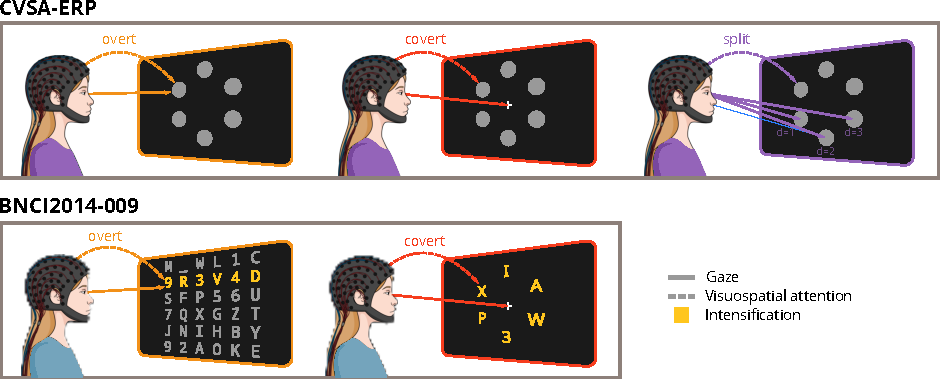
\includegraphics[width=\linewidth]{figures/covert_align/dataset_vsa.pdf}
    \caption[Dataset stimulation interfaces.]{%
    Interfaces and visuospatial attention (\ac{vsa})
    conditions in the CVSA-ERP and BNCI2014-009 datasets.
		In the CVSA-ERP oddball \ac{bci} interface, screen targets are intensified one after
    the other in pseudorandom order while the participant can either pay overt,
    covert, or split \ac{vsa} to the cued target.
		In the BNCI2014-009 overt \ac{vsa} interface, entire rows and columns are
		intensified at once. In its covert counterpart,
		groups of 6 letters are intensified one after the other, partly relying on
    feature attention.

    }%
		\label{fig:interface}
\end{figure*}
\begin{figure*}[t]
  \input{figures/covert_align/grand_avg.pfg}
	%\includegraphics[width=\linewidth]{figures/covert_align/figure3b.pdf}
  \caption[Evoked \acs{erp} per dataset and condition.]{%
		Contrast between target (color) and non-target, and
    distractor (gray) and non-target grand average event-related potentials per \ac{vsa} condition and dataset.
    Overt \ac{vsa} yields a strong modulation of the N1 component in both datasets;
    the P3 amplitude decreases with the degree of split \ac{vsa}.
    In split \ac{vsa}, N1 and P2 are more prominently evoked by the distractor,
    while the P3 is evoked by the target.
	}
		\label{fig:erps}
\end{figure*}


In contrast to the protocol proposed by \textcite{Frenzel2011}, split \ac{vsa} was
performed by instructing the participant to attend to the intensifications of the
cued target and ignore the intensifications of the distractor target.
Since we assume there will be an effect depending on the distance between
the attended target and the distractor, we discern three split \ac{vsa} sub-conditions:
the distractor is either clockwise or counterclockwise directly next to the
attended target ($d=1$), there is one other target between the attended target and
the distractor ($d=2$), or the distractor is opposite the intended target
($d=3$).

\ac{eeg} for the CVSA-ERP dataset was recorded using a SynAmps RT amplifier
(Compumedics Neuroscan, Australia) at 2048 Hz and 62 Ag/AgCl active electrodes arranged in the
international 10-10 layout fitted to a standard electrode cap (EASYCAP GmbH,
Germany), with electrodes located at AFz and FCz as ground and reference, respectively.
Using electrolyte gel, electrode impedances were brought below 5k$\Omega$.
Electrodes TP9 and TP10, used for off-line re-referencing, were directly
attached to the skin using stickers for better contact.
The power line frequency in Belgium is 50 Hz.
The participant's eye gaze was registered using an EyeLink 1000 Plus eye tracker (SR Research,
Canada) in non-fixation mode.

Participants signed an informed consent form and were seated at a distance of
60 cm from a CRT-emulating monitor (VPixx
Technologies, Ca\-na\-da) operating at a refresh rate of 120 Hz, displaying 6
circular white targets with a diameter of 4.15° visual angle and laid out on a hexagon
with a radius of 12.28° of visual angle centered on the midpoint of the screen,
conforming to the interface proposed by \textcite{Treder2010}
(\cref{fig:covert-align/interface/interface}).
A hexagonal layout interface with an empty center and a low number of targets
counteracts target crowding, and as long as the subject’s gaze is within the hexagon of
targets, no other target can be between the subject’s gaze and a covertly
attended target.
Targets are full-contrast white and were intensified by scaling them to a
larger size (5.60° of visual angle, see \cref{fig:covert-align/interface/intensification})
instead of changing the contrast to avoid Troxler-fading\footnote{The optical illusion of disappearing unchanging stimuli
experienced when visually fixating~\cite{Troxler1804}.}~\cite{Treder2010} in the
peripheral visual field.
Stimuli were presented using PsychoPy (version 2023.1.3)~\cite{Peirce2019}.

\begin{figure}[t]
  \begin{subfigure}[t]{.45\textwidth}
    \input{figures/covert_align/interface_1.tikz.tex}
    \caption[The stimulation interface.]{The stimulation interface based on the visual Hex-o-Spell
    \acs{bci}~\cite{Treder2010}.}%
    \label{fig:covert-align/interface/interface}
  \end{subfigure}\hfill%
  \begin{subfigure}[t]{.45\textwidth}
    \begin{tikzpicture}[
    scale=\textwidth/5cm
]
% Rectangle background
\fill[muteblack] (-2.5,-2) rectangle (2.5,2);

% Hexagon vertices (white circles)
\fill[white] (1,0) circle (.35);    % Right
\fill[white] (-1,0) circle (.35);   % Left
\fill[white] (0.5,0.866) circle (.35); % Top-right
\fill[white] (-0.5,0.866) circle (.45); % Top-left
\fill[white] (0.5,-0.866) circle (.35); % Bottom-right
\fill[white] (-0.5,-0.866) circle (.35); % Bottom-left

\end{tikzpicture}%

    \caption[Intensification.]{When a target is intensified, it is enlarged for
    a very short time.}%
    \label{fig:covert-align/interface/intensification}
  \end{subfigure}

  \bigskip

  \begin{subfigure}[t]{.45\textwidth}
    \begin{tikzpicture}[
    scale=\textwidth/5cm
]
% Rectangle background
\fill[muteblack] (-2.5,-2) rectangle (2.5,2);

% Hexagon vertices (white circles)
\fill[white] (1,0) circle (.35);    % Right
\fill[white] (-1,0) circle (.35);   % Left
\fill[white] (0.5,0.866) circle (.35); % Top-right
\fill[white] (-0.5,0.866) circle (.35); % Top-left
\fill[white] (0.5,-0.866) circle (.35); % Bottom-right
\fill[white] (-0.5,-0.866) circle (.35); % Bottom-left
\draw[accent2, ultra thick] (0.9,0) -- (1.1,0);  % Shorter horizontal line
\draw[accent2, ultra thick] (1,-0.1) -- (1,0.1); % Shorter vertical line
\end{tikzpicture}%

    \caption[Gaze fixated on a target.]{In the overt and split \ac{vsa}
    settings, the
    participant is cued to fixate on one of the targets.}%
    \label{fig:covert-align/interface/overt}
  \end{subfigure}\hfill%
  \begin{subfigure}[t]{.45\textwidth}
    \begin{tikzpicture}[
    scale=\textwidth/5cm
]
% Rectangle background
\fill[muteblack] (-2.5,-2) rectangle (2.5,2);

% Hexagon vertices (white circles)
\fill[white] (1,0) circle (.35);    % Right
\fill[white] (-1,0) circle (.35);   % Left
\fill[white] (0.5,0.866) circle (.35); % Top-right
\fill[white] (-0.5,0.866) circle (.35); % Top-left
\fill[white] (0.5,-0.866) circle (.35); % Bottom-right
\fill[white] (-0.5,-0.866) circle (.35); % Bottom-left

% Plus symbol made of two shorter lines at the center (0,0)
\draw[accent2, ultra thick] (-0.1,0) -- (0.1,0);  % Shorter horizontal line
\draw[accent2, ultra thick] (0,-0.1) -- (0,0.1);  % Shorter vertical line
\end{tikzpicture}%

    \caption[Gaze fixated centrally.]{In the covert \ac{vsa} setting, the participant is
    cued to fixate at the center of the interface.}%
    \label{fig:covert-align/interface/covert}
  \end{subfigure}
  \caption[Stimulation interface layout.]{Layout and visual elements of the experimental stimulation
  interface used in recording the CVSA-ERP dataset.}
\end{figure}

The participant was instructed to press the space bar when ready for a block
of stimulations.
Then, one target was indicated as the cue, and the participant
was instructed to count the number of intensifications of the cued target
during the following block of stimulations.
After pressing the space bar again, a blue crosshair appeared, and the subject
was instructed to fixate their gaze on the blue crosshair for the duration of
the stimulation block (\cref{fig:covert-align/interface/overt} and
\cref{fig:covert-align/interface/covert}).
The position of this crosshair determined the \ac{vsa} condition for this trial:
overt \ac{vsa} when the crosshair was at the same location as the cued target,
covert \ac{vsa} when the crosshair appeared in the center of the screen, and split
\ac{vsa} when the crosshair appeared on a different target than the cued one.
After pressing the space bar again and a delay of 5 seconds, the stimulation block
started.

All targets were intensified for a duration of 100 ms in pseudorandom order.
The inter-stimulus-interval (\ac{isi}), the time between the onsets of subsequent intensifications,
was variable and consisted of a fixed 300 ms interval (of which 100 ms with an intensified target onscreen)
with 200 ms of uniform jitter added, resulting in an \ac{isi}
between 200 and 400 ms.
\Acp{isi} were jittered to counteract steady-state effects and residue in averaging. A
longer \ac{isi} will increase component amplitude and aid in counteracting temporal
autocorrelation for higher statistical test precision.
In a block of stimulations, each target was intensified a pseudorandom number of times between 10 and 15.
This led to stimulation blocks with an average duration of 26.25 seconds. After a block of stimulations, an
input prompt appeared to enter the mentally counted number of intensifications.
After inputting this number, the subject was allowed to pause until pressing the space bar again.
In total, six blocks were presented for overt \ac{vsa}, six blocks for covert \ac{vsa}, 12 blocks for
split ($d=1$) \ac{vsa}, 12 blocks for split ($d=2$) \ac{vsa}, and 6 blocks for split
($d=3$) \ac{vsa}, covering all possible combinations of \ac{vsa} conditions, cued targets, and
crosshair locations.

The experiment started with a sequence  of five non-recorded practice stimulation blocks, one for
each of the five \ac{vsa} conditions.
During these practice blocks, the participant received feedback about their gaze
position and counting accuracy.
Counting the instructions and the participant's response to the
input prompts, a block lasted about 30 seconds. In sum, the experiment featured approximately 45 minutes of
stimulation time.
After blocks 14 and 28, the participant was allowed to take a longer break.
Including these longer breaks, the experiment lasted approximately one hour.

\subsubsection{BNCI2014-009 dataset}
The BNCI2014-009\footnote{\url{https://bnci-horizon-2020.eu/database/data-sets}}
dataset~\cite{Aloise2012a} was used in the analysis performed
by \textcite{Arico2014}.
It contains data from 10 subjects (median age $24.5\pm1.9$
years) who performed two spelling tasks illustrated in the second row of
\cref{fig:interface}: using the P3 Matrix speller
interface to exploit overt \ac{vsa}, and the GeoSpell covert \ac{vsa} interface.
To use the GeoSpell interface, the participant gazes at the fixation point at the
center of the screen, while groups of characters flash simultaneously in a
circular layout around the fixation point.
The user directs their visuospatial attention to the location where the intended letter is expected
to appear, and when it does, a P3 \ac{erp} component is expected to be evoked.
This results in a specific setting where both visuospatial attention and
feature attention (the attended letter) are exploited.
For a detailed description of the paradigm and dataset, we refer
to \textcite{Aloise2012a}.

\subsection{Data processing and analysis}
\subsubsection{Preprocessing}
Analysis was performed using Python and the MNE software package (version
1.3.1)~\cite{Gramfort2013}.
All datasets were band-pass filtered between 0.1 Hz and 20 Hz with a 4th-order Butterworth filter.
Bad channels in the data were automatically detected using the RANSAC
method~\cite{Fischler1981} and rejected.
The recorded \ac{eeg} was re-referenced
offline to the average of the mastoid electrodes TP9 and TP10.
Next, the \ac{eeg} signals were corrected for eye movement artifacts using
Independent Component Analysis (ICA).
Since we have access to \ac{eog} data for the CVSA-ERP dataset, components correlating
significantly with the \ac{eog} were rejected.
For the BNCI2014-009 dataset, ICA components were manually rejected.
Finally, the \ac{eeg} signal was divided into epochs ranging from 100 ms before stimulus onset to 700 ms after stimulus onset and down-sampled to 128 Hz.
In both datasets, only 16 channels were kept for
analysis (Fz, FCz, Cz, CPz, Pz, Oz, F3, F4, C3, C4, CP3, CP4, P3, P4, PO7, and
PO8).

\subsubsection{Decoders}%
\label{sec:covert-align/methods/decoders}
We compared \ac{wcble} and \ac{cble} as described in
\cref{sec:wcble/methods}, with their base classifier \ac{tlda} and with
Riemannian Geometry approaches that rely on spatial covariance as features.
Together with \ac{tlda}, Riemannian Geometry generally achieves state-of-the-art decoding
performance~\cite{Lotte2018}.
We implemented two Riemannian Geometry pipelines.
The first estimates shrunk covariances from the \acp{erp} filtered with 6 XDAWN
filters, projects these covariances to a tangent space, and classifies the
result using $L_2$-regularized logistic regression
(XDAWNCov-TS-LR)~\cite{Cecotti2017}.
Secondly, we adopted the pipeline from \textcite{Aydarkhanov2020}, as their work shows
favorable performance in the presence of single-trial \ac{erp} latency jitter.
Shrunk spatial covariance matrices were estimated from epochs that were
augmented by concatenating the average target and average non-target \ac{erp} as
extra channels, projected to tangent space, and classified using
$L_2$-regularized logistic regression (ERPCov-TS-LR).

To evaluate performance, 6-fold cross-validation without shuffling was performed for both
datasets.
At each fold, classifiers were trained on five target selection blocks (300
epochs) and tested on one block (60 epochs) without overlap for CVSA-ERP.
For each subject and run in the BNCI2014-009 dataset, classifiers
were trained on five symbol selections (480 epochs) and tested on one symbol
selection (96 epochs) without overlap at each fold.
A window ranging from 0 ms to 600 ms after stimulus onset was used for \ac{cble} and \ac{wcble}.
With epochs ranging from -100 ms to 700 ms relative to stimulus onset, this
allows for extracting latencies ranging from -100 ms to +100 ms.


\section{Results}

\subsection{\Acs{bci} decoding performance}%
\label{sec:covert-align/results/bloc-acc}

We evaluated the \ac{bci} decoding performance in a single-trial classification
experiment, as well as in a target selection experiment reflecting \ac{bci}
operation.

\Cref{fig:covert-align/single-trial-roc-auc-diff} shows a comparison of \ac{rocauc}
for all pairs of \ac{tlda}, \ac{cble},
and \ac{wcble} for single-trial classification to investigate the contributions of
\ac{cble} and \ac{wcble} relative to their first-stage classifier \ac{tlda}.
For this evaluation, epochs were rejected when the peak-to-peak amplitude
exceeded 800 µV, and for the CVSA-ERP dataset, if the user's gaze differed by more than
10 degrees of visual angle from the fixation crosshair.
\begin{figure}[t]
	%\includegraphics[width=\linewidth]{figures/covert_align/figure4a.pdf}
  \hspace{-0.6818736741559431in}
%%% Creator: Matplotlib, PGF backend
%%
%% To include the figure in your LaTeX document, write
%%   \input{<filename>.pgf}
%%
%% Make sure the required packages are loaded in your preamble
%%   \usepackage{pgf}
%%
%% Also ensure that all the required font packages are loaded; for instance,
%% the lmodern package is sometimes necessary when using math font.
%%   \usepackage{lmodern}
%%
%% Figures using additional raster images can only be included by \input if
%% they are in the same directory as the main LaTeX file. For loading figures
%% from other directories you can use the `import` package
%%   \usepackage{import}
%%
%% and then include the figures with
%%   \import{<path to file>}{<filename>.pgf}
%%
%% Matplotlib used the following preamble
%%   \def\mathdefault#1{#1}
%%   \everymath=\expandafter{\the\everymath\displaystyle}
%%   
%%   \ifdefined\pdftexversion\else  % non-pdftex case.
%%     \usepackage{fontspec}
%%   \fi
%%   \makeatletter\@ifpackageloaded{underscore}{}{\usepackage[strings]{underscore}}\makeatother
%%
\begingroup%
\makeatletter%
\begin{pgfpicture}%
\pgfpathrectangle{\pgfpointorigin}{\pgfqpoint{5.322943in}{1.863224in}}%
\pgfusepath{use as bounding box, clip}%
\begin{pgfscope}%
\pgfsetbuttcap%
\pgfsetmiterjoin%
\pgfsetlinewidth{0.000000pt}%
\definecolor{currentstroke}{rgb}{1.000000,1.000000,1.000000}%
\pgfsetstrokecolor{currentstroke}%
\pgfsetstrokeopacity{0.000000}%
\pgfsetdash{}{0pt}%
\pgfpathmoveto{\pgfqpoint{0.000000in}{0.000000in}}%
\pgfpathlineto{\pgfqpoint{5.322943in}{0.000000in}}%
\pgfpathlineto{\pgfqpoint{5.322943in}{1.863224in}}%
\pgfpathlineto{\pgfqpoint{0.000000in}{1.863224in}}%
\pgfpathlineto{\pgfqpoint{0.000000in}{0.000000in}}%
\pgfpathclose%
\pgfusepath{}%
\end{pgfscope}%
\begin{pgfscope}%
\pgfsetbuttcap%
\pgfsetmiterjoin%
\definecolor{currentfill}{rgb}{1.000000,1.000000,1.000000}%
\pgfsetfillcolor{currentfill}%
\pgfsetlinewidth{0.000000pt}%
\definecolor{currentstroke}{rgb}{0.000000,0.000000,0.000000}%
\pgfsetstrokecolor{currentstroke}%
\pgfsetstrokeopacity{0.000000}%
\pgfsetdash{}{0pt}%
\pgfpathmoveto{\pgfqpoint{0.716792in}{0.897930in}}%
\pgfpathlineto{\pgfqpoint{2.196615in}{0.897930in}}%
\pgfpathlineto{\pgfqpoint{2.196615in}{1.693085in}}%
\pgfpathlineto{\pgfqpoint{0.716792in}{1.693085in}}%
\pgfpathlineto{\pgfqpoint{0.716792in}{0.897930in}}%
\pgfpathclose%
\pgfusepath{fill}%
\end{pgfscope}%
\begin{pgfscope}%
\pgfpathrectangle{\pgfqpoint{0.716792in}{0.897930in}}{\pgfqpoint{1.479824in}{0.795155in}}%
\pgfusepath{clip}%
\pgfsetbuttcap%
\pgfsetroundjoin%
\pgfsetlinewidth{1.003750pt}%
\definecolor{currentstroke}{rgb}{0.878431,0.878431,0.878431}%
\pgfsetstrokecolor{currentstroke}%
\pgfsetdash{{3.700000pt}{1.600000pt}}{0.000000pt}%
\pgfpathmoveto{\pgfqpoint{1.456704in}{0.897930in}}%
\pgfpathlineto{\pgfqpoint{1.456704in}{1.693085in}}%
\pgfusepath{stroke}%
\end{pgfscope}%
\begin{pgfscope}%
\pgfpathrectangle{\pgfqpoint{0.716792in}{0.897930in}}{\pgfqpoint{1.479824in}{0.795155in}}%
\pgfusepath{clip}%
\pgfsetbuttcap%
\pgfsetroundjoin%
\definecolor{currentfill}{rgb}{0.827451,0.827451,0.827451}%
\pgfsetfillcolor{currentfill}%
\pgfsetlinewidth{0.000000pt}%
\definecolor{currentstroke}{rgb}{0.496471,0.496471,0.496471}%
\pgfsetstrokecolor{currentstroke}%
\pgfsetdash{}{0pt}%
\pgfsys@defobject{currentmarker}{\pgfqpoint{-0.020833in}{-0.020833in}}{\pgfqpoint{0.020833in}{0.020833in}}{%
\pgfpathmoveto{\pgfqpoint{0.000000in}{-0.020833in}}%
\pgfpathcurveto{\pgfqpoint{0.005525in}{-0.020833in}}{\pgfqpoint{0.010825in}{-0.018638in}}{\pgfqpoint{0.014731in}{-0.014731in}}%
\pgfpathcurveto{\pgfqpoint{0.018638in}{-0.010825in}}{\pgfqpoint{0.020833in}{-0.005525in}}{\pgfqpoint{0.020833in}{0.000000in}}%
\pgfpathcurveto{\pgfqpoint{0.020833in}{0.005525in}}{\pgfqpoint{0.018638in}{0.010825in}}{\pgfqpoint{0.014731in}{0.014731in}}%
\pgfpathcurveto{\pgfqpoint{0.010825in}{0.018638in}}{\pgfqpoint{0.005525in}{0.020833in}}{\pgfqpoint{0.000000in}{0.020833in}}%
\pgfpathcurveto{\pgfqpoint{-0.005525in}{0.020833in}}{\pgfqpoint{-0.010825in}{0.018638in}}{\pgfqpoint{-0.014731in}{0.014731in}}%
\pgfpathcurveto{\pgfqpoint{-0.018638in}{0.010825in}}{\pgfqpoint{-0.020833in}{0.005525in}}{\pgfqpoint{-0.020833in}{0.000000in}}%
\pgfpathcurveto{\pgfqpoint{-0.020833in}{-0.005525in}}{\pgfqpoint{-0.018638in}{-0.010825in}}{\pgfqpoint{-0.014731in}{-0.014731in}}%
\pgfpathcurveto{\pgfqpoint{-0.010825in}{-0.018638in}}{\pgfqpoint{-0.005525in}{-0.020833in}}{\pgfqpoint{0.000000in}{-0.020833in}}%
\pgfpathlineto{\pgfqpoint{0.000000in}{-0.020833in}}%
\pgfpathclose%
\pgfusepath{fill}%
}%
\begin{pgfscope}%
\pgfsys@transformshift{1.350650in}{1.608324in}%
\pgfsys@useobject{currentmarker}{}%
\end{pgfscope}%
\begin{pgfscope}%
\pgfsys@transformshift{1.801996in}{1.621642in}%
\pgfsys@useobject{currentmarker}{}%
\end{pgfscope}%
\begin{pgfscope}%
\pgfsys@transformshift{1.370381in}{1.613072in}%
\pgfsys@useobject{currentmarker}{}%
\end{pgfscope}%
\begin{pgfscope}%
\pgfsys@transformshift{1.834059in}{1.628159in}%
\pgfsys@useobject{currentmarker}{}%
\end{pgfscope}%
\begin{pgfscope}%
\pgfsys@transformshift{1.613897in}{1.607245in}%
\pgfsys@useobject{currentmarker}{}%
\end{pgfscope}%
\begin{pgfscope}%
\pgfsys@transformshift{1.459170in}{1.615064in}%
\pgfsys@useobject{currentmarker}{}%
\end{pgfscope}%
\begin{pgfscope}%
\pgfsys@transformshift{2.132490in}{1.599540in}%
\pgfsys@useobject{currentmarker}{}%
\end{pgfscope}%
\begin{pgfscope}%
\pgfsys@transformshift{1.789664in}{1.625868in}%
\pgfsys@useobject{currentmarker}{}%
\end{pgfscope}%
\begin{pgfscope}%
\pgfsys@transformshift{1.656480in}{1.610811in}%
\pgfsys@useobject{currentmarker}{}%
\end{pgfscope}%
\begin{pgfscope}%
\pgfsys@transformshift{1.454237in}{1.597740in}%
\pgfsys@useobject{currentmarker}{}%
\end{pgfscope}%
\begin{pgfscope}%
\pgfsys@transformshift{1.407376in}{1.617400in}%
\pgfsys@useobject{currentmarker}{}%
\end{pgfscope}%
\begin{pgfscope}%
\pgfsys@transformshift{1.417242in}{1.626332in}%
\pgfsys@useobject{currentmarker}{}%
\end{pgfscope}%
\begin{pgfscope}%
\pgfsys@transformshift{1.535628in}{1.606925in}%
\pgfsys@useobject{currentmarker}{}%
\end{pgfscope}%
\begin{pgfscope}%
\pgfsys@transformshift{0.896837in}{1.607830in}%
\pgfsys@useobject{currentmarker}{}%
\end{pgfscope}%
\begin{pgfscope}%
\pgfsys@transformshift{1.628544in}{1.611419in}%
\pgfsys@useobject{currentmarker}{}%
\end{pgfscope}%
\end{pgfscope}%
\begin{pgfscope}%
\pgfpathrectangle{\pgfqpoint{0.716792in}{0.897930in}}{\pgfqpoint{1.479824in}{0.795155in}}%
\pgfusepath{clip}%
\pgfsetbuttcap%
\pgfsetroundjoin%
\definecolor{currentfill}{rgb}{0.827451,0.827451,0.827451}%
\pgfsetfillcolor{currentfill}%
\pgfsetlinewidth{0.000000pt}%
\definecolor{currentstroke}{rgb}{0.496471,0.496471,0.496471}%
\pgfsetstrokecolor{currentstroke}%
\pgfsetdash{}{0pt}%
\pgfsys@defobject{currentmarker}{\pgfqpoint{-0.020833in}{-0.020833in}}{\pgfqpoint{0.020833in}{0.020833in}}{%
\pgfpathmoveto{\pgfqpoint{0.000000in}{-0.020833in}}%
\pgfpathcurveto{\pgfqpoint{0.005525in}{-0.020833in}}{\pgfqpoint{0.010825in}{-0.018638in}}{\pgfqpoint{0.014731in}{-0.014731in}}%
\pgfpathcurveto{\pgfqpoint{0.018638in}{-0.010825in}}{\pgfqpoint{0.020833in}{-0.005525in}}{\pgfqpoint{0.020833in}{0.000000in}}%
\pgfpathcurveto{\pgfqpoint{0.020833in}{0.005525in}}{\pgfqpoint{0.018638in}{0.010825in}}{\pgfqpoint{0.014731in}{0.014731in}}%
\pgfpathcurveto{\pgfqpoint{0.010825in}{0.018638in}}{\pgfqpoint{0.005525in}{0.020833in}}{\pgfqpoint{0.000000in}{0.020833in}}%
\pgfpathcurveto{\pgfqpoint{-0.005525in}{0.020833in}}{\pgfqpoint{-0.010825in}{0.018638in}}{\pgfqpoint{-0.014731in}{0.014731in}}%
\pgfpathcurveto{\pgfqpoint{-0.018638in}{0.010825in}}{\pgfqpoint{-0.020833in}{0.005525in}}{\pgfqpoint{-0.020833in}{0.000000in}}%
\pgfpathcurveto{\pgfqpoint{-0.020833in}{-0.005525in}}{\pgfqpoint{-0.018638in}{-0.010825in}}{\pgfqpoint{-0.014731in}{-0.014731in}}%
\pgfpathcurveto{\pgfqpoint{-0.010825in}{-0.018638in}}{\pgfqpoint{-0.005525in}{-0.020833in}}{\pgfqpoint{0.000000in}{-0.020833in}}%
\pgfpathlineto{\pgfqpoint{0.000000in}{-0.020833in}}%
\pgfpathclose%
\pgfusepath{fill}%
}%
\begin{pgfscope}%
\pgfsys@transformshift{1.392578in}{1.469402in}%
\pgfsys@useobject{currentmarker}{}%
\end{pgfscope}%
\begin{pgfscope}%
\pgfsys@transformshift{1.530695in}{1.444092in}%
\pgfsys@useobject{currentmarker}{}%
\end{pgfscope}%
\begin{pgfscope}%
\pgfsys@transformshift{1.215553in}{1.445313in}%
\pgfsys@useobject{currentmarker}{}%
\end{pgfscope}%
\begin{pgfscope}%
\pgfsys@transformshift{1.010290in}{1.462028in}%
\pgfsys@useobject{currentmarker}{}%
\end{pgfscope}%
\begin{pgfscope}%
\pgfsys@transformshift{1.432040in}{1.461547in}%
\pgfsys@useobject{currentmarker}{}%
\end{pgfscope}%
\begin{pgfscope}%
\pgfsys@transformshift{1.472106in}{1.458179in}%
\pgfsys@useobject{currentmarker}{}%
\end{pgfscope}%
\begin{pgfscope}%
\pgfsys@transformshift{1.422174in}{1.446094in}%
\pgfsys@useobject{currentmarker}{}%
\end{pgfscope}%
\begin{pgfscope}%
\pgfsys@transformshift{1.217465in}{1.465567in}%
\pgfsys@useobject{currentmarker}{}%
\end{pgfscope}%
\begin{pgfscope}%
\pgfsys@transformshift{1.666345in}{1.448502in}%
\pgfsys@useobject{currentmarker}{}%
\end{pgfscope}%
\begin{pgfscope}%
\pgfsys@transformshift{0.768586in}{1.466642in}%
\pgfsys@useobject{currentmarker}{}%
\end{pgfscope}%
\begin{pgfscope}%
\pgfsys@transformshift{1.572623in}{1.463696in}%
\pgfsys@useobject{currentmarker}{}%
\end{pgfscope}%
\begin{pgfscope}%
\pgfsys@transformshift{1.002891in}{1.448768in}%
\pgfsys@useobject{currentmarker}{}%
\end{pgfscope}%
\begin{pgfscope}%
\pgfsys@transformshift{1.264326in}{1.443837in}%
\pgfsys@useobject{currentmarker}{}%
\end{pgfscope}%
\begin{pgfscope}%
\pgfsys@transformshift{1.427107in}{1.461704in}%
\pgfsys@useobject{currentmarker}{}%
\end{pgfscope}%
\begin{pgfscope}%
\pgfsys@transformshift{0.933832in}{1.464865in}%
\pgfsys@useobject{currentmarker}{}%
\end{pgfscope}%
\end{pgfscope}%
\begin{pgfscope}%
\pgfpathrectangle{\pgfqpoint{0.716792in}{0.897930in}}{\pgfqpoint{1.479824in}{0.795155in}}%
\pgfusepath{clip}%
\pgfsetbuttcap%
\pgfsetroundjoin%
\definecolor{currentfill}{rgb}{0.827451,0.827451,0.827451}%
\pgfsetfillcolor{currentfill}%
\pgfsetlinewidth{0.000000pt}%
\definecolor{currentstroke}{rgb}{0.496471,0.496471,0.496471}%
\pgfsetstrokecolor{currentstroke}%
\pgfsetdash{}{0pt}%
\pgfsys@defobject{currentmarker}{\pgfqpoint{-0.020833in}{-0.020833in}}{\pgfqpoint{0.020833in}{0.020833in}}{%
\pgfpathmoveto{\pgfqpoint{0.000000in}{-0.020833in}}%
\pgfpathcurveto{\pgfqpoint{0.005525in}{-0.020833in}}{\pgfqpoint{0.010825in}{-0.018638in}}{\pgfqpoint{0.014731in}{-0.014731in}}%
\pgfpathcurveto{\pgfqpoint{0.018638in}{-0.010825in}}{\pgfqpoint{0.020833in}{-0.005525in}}{\pgfqpoint{0.020833in}{0.000000in}}%
\pgfpathcurveto{\pgfqpoint{0.020833in}{0.005525in}}{\pgfqpoint{0.018638in}{0.010825in}}{\pgfqpoint{0.014731in}{0.014731in}}%
\pgfpathcurveto{\pgfqpoint{0.010825in}{0.018638in}}{\pgfqpoint{0.005525in}{0.020833in}}{\pgfqpoint{0.000000in}{0.020833in}}%
\pgfpathcurveto{\pgfqpoint{-0.005525in}{0.020833in}}{\pgfqpoint{-0.010825in}{0.018638in}}{\pgfqpoint{-0.014731in}{0.014731in}}%
\pgfpathcurveto{\pgfqpoint{-0.018638in}{0.010825in}}{\pgfqpoint{-0.020833in}{0.005525in}}{\pgfqpoint{-0.020833in}{0.000000in}}%
\pgfpathcurveto{\pgfqpoint{-0.020833in}{-0.005525in}}{\pgfqpoint{-0.018638in}{-0.010825in}}{\pgfqpoint{-0.014731in}{-0.014731in}}%
\pgfpathcurveto{\pgfqpoint{-0.010825in}{-0.018638in}}{\pgfqpoint{-0.005525in}{-0.020833in}}{\pgfqpoint{0.000000in}{-0.020833in}}%
\pgfpathlineto{\pgfqpoint{0.000000in}{-0.020833in}}%
\pgfpathclose%
\pgfusepath{fill}%
}%
\begin{pgfscope}%
\pgfsys@transformshift{1.638119in}{1.301959in}%
\pgfsys@useobject{currentmarker}{}%
\end{pgfscope}%
\begin{pgfscope}%
\pgfsys@transformshift{1.362981in}{1.306413in}%
\pgfsys@useobject{currentmarker}{}%
\end{pgfscope}%
\begin{pgfscope}%
\pgfsys@transformshift{1.678677in}{1.290734in}%
\pgfsys@useobject{currentmarker}{}%
\end{pgfscope}%
\begin{pgfscope}%
\pgfsys@transformshift{0.941232in}{1.304977in}%
\pgfsys@useobject{currentmarker}{}%
\end{pgfscope}%
\begin{pgfscope}%
\pgfsys@transformshift{1.158272in}{1.291501in}%
\pgfsys@useobject{currentmarker}{}%
\end{pgfscope}%
\begin{pgfscope}%
\pgfsys@transformshift{1.007824in}{1.309793in}%
\pgfsys@useobject{currentmarker}{}%
\end{pgfscope}%
\begin{pgfscope}%
\pgfsys@transformshift{1.905583in}{1.296123in}%
\pgfsys@useobject{currentmarker}{}%
\end{pgfscope}%
\begin{pgfscope}%
\pgfsys@transformshift{1.321053in}{1.301076in}%
\pgfsys@useobject{currentmarker}{}%
\end{pgfscope}%
\begin{pgfscope}%
\pgfsys@transformshift{1.920382in}{1.305177in}%
\pgfsys@useobject{currentmarker}{}%
\end{pgfscope}%
\begin{pgfscope}%
\pgfsys@transformshift{2.063431in}{1.280525in}%
\pgfsys@useobject{currentmarker}{}%
\end{pgfscope}%
\begin{pgfscope}%
\pgfsys@transformshift{1.333385in}{1.297241in}%
\pgfsys@useobject{currentmarker}{}%
\end{pgfscope}%
\begin{pgfscope}%
\pgfsys@transformshift{1.311188in}{1.310060in}%
\pgfsys@useobject{currentmarker}{}%
\end{pgfscope}%
\begin{pgfscope}%
\pgfsys@transformshift{1.614551in}{1.300030in}%
\pgfsys@useobject{currentmarker}{}%
\end{pgfscope}%
\begin{pgfscope}%
\pgfsys@transformshift{1.423986in}{1.304732in}%
\pgfsys@useobject{currentmarker}{}%
\end{pgfscope}%
\begin{pgfscope}%
\pgfsys@transformshift{1.321053in}{1.292058in}%
\pgfsys@useobject{currentmarker}{}%
\end{pgfscope}%
\end{pgfscope}%
\begin{pgfscope}%
\pgfpathrectangle{\pgfqpoint{0.716792in}{0.897930in}}{\pgfqpoint{1.479824in}{0.795155in}}%
\pgfusepath{clip}%
\pgfsetbuttcap%
\pgfsetroundjoin%
\definecolor{currentfill}{rgb}{0.827451,0.827451,0.827451}%
\pgfsetfillcolor{currentfill}%
\pgfsetlinewidth{0.000000pt}%
\definecolor{currentstroke}{rgb}{0.496471,0.496471,0.496471}%
\pgfsetstrokecolor{currentstroke}%
\pgfsetdash{}{0pt}%
\pgfsys@defobject{currentmarker}{\pgfqpoint{-0.020833in}{-0.020833in}}{\pgfqpoint{0.020833in}{0.020833in}}{%
\pgfpathmoveto{\pgfqpoint{0.000000in}{-0.020833in}}%
\pgfpathcurveto{\pgfqpoint{0.005525in}{-0.020833in}}{\pgfqpoint{0.010825in}{-0.018638in}}{\pgfqpoint{0.014731in}{-0.014731in}}%
\pgfpathcurveto{\pgfqpoint{0.018638in}{-0.010825in}}{\pgfqpoint{0.020833in}{-0.005525in}}{\pgfqpoint{0.020833in}{0.000000in}}%
\pgfpathcurveto{\pgfqpoint{0.020833in}{0.005525in}}{\pgfqpoint{0.018638in}{0.010825in}}{\pgfqpoint{0.014731in}{0.014731in}}%
\pgfpathcurveto{\pgfqpoint{0.010825in}{0.018638in}}{\pgfqpoint{0.005525in}{0.020833in}}{\pgfqpoint{0.000000in}{0.020833in}}%
\pgfpathcurveto{\pgfqpoint{-0.005525in}{0.020833in}}{\pgfqpoint{-0.010825in}{0.018638in}}{\pgfqpoint{-0.014731in}{0.014731in}}%
\pgfpathcurveto{\pgfqpoint{-0.018638in}{0.010825in}}{\pgfqpoint{-0.020833in}{0.005525in}}{\pgfqpoint{-0.020833in}{0.000000in}}%
\pgfpathcurveto{\pgfqpoint{-0.020833in}{-0.005525in}}{\pgfqpoint{-0.018638in}{-0.010825in}}{\pgfqpoint{-0.014731in}{-0.014731in}}%
\pgfpathcurveto{\pgfqpoint{-0.010825in}{-0.018638in}}{\pgfqpoint{-0.005525in}{-0.020833in}}{\pgfqpoint{0.000000in}{-0.020833in}}%
\pgfpathlineto{\pgfqpoint{0.000000in}{-0.020833in}}%
\pgfpathclose%
\pgfusepath{fill}%
}%
\begin{pgfscope}%
\pgfsys@transformshift{1.180470in}{1.138119in}%
\pgfsys@useobject{currentmarker}{}%
\end{pgfscope}%
\begin{pgfscope}%
\pgfsys@transformshift{0.938765in}{1.132519in}%
\pgfsys@useobject{currentmarker}{}%
\end{pgfscope}%
\begin{pgfscope}%
\pgfsys@transformshift{1.459170in}{1.126488in}%
\pgfsys@useobject{currentmarker}{}%
\end{pgfscope}%
\begin{pgfscope}%
\pgfsys@transformshift{1.597287in}{1.148844in}%
\pgfsys@useobject{currentmarker}{}%
\end{pgfscope}%
\begin{pgfscope}%
\pgfsys@transformshift{1.533161in}{1.148513in}%
\pgfsys@useobject{currentmarker}{}%
\end{pgfscope}%
\begin{pgfscope}%
\pgfsys@transformshift{1.173071in}{1.145616in}%
\pgfsys@useobject{currentmarker}{}%
\end{pgfscope}%
\begin{pgfscope}%
\pgfsys@transformshift{1.525762in}{1.147518in}%
\pgfsys@useobject{currentmarker}{}%
\end{pgfscope}%
\begin{pgfscope}%
\pgfsys@transformshift{1.305600in}{1.126011in}%
\pgfsys@useobject{currentmarker}{}%
\end{pgfscope}%
\begin{pgfscope}%
\pgfsys@transformshift{1.836525in}{1.123810in}%
\pgfsys@useobject{currentmarker}{}%
\end{pgfscope}%
\begin{pgfscope}%
\pgfsys@transformshift{1.508497in}{1.126451in}%
\pgfsys@useobject{currentmarker}{}%
\end{pgfscope}%
\begin{pgfscope}%
\pgfsys@transformshift{1.434506in}{1.144208in}%
\pgfsys@useobject{currentmarker}{}%
\end{pgfscope}%
\begin{pgfscope}%
\pgfsys@transformshift{1.528228in}{1.129815in}%
\pgfsys@useobject{currentmarker}{}%
\end{pgfscope}%
\begin{pgfscope}%
\pgfsys@transformshift{1.646665in}{1.149155in}%
\pgfsys@useobject{currentmarker}{}%
\end{pgfscope}%
\begin{pgfscope}%
\pgfsys@transformshift{1.427107in}{1.122899in}%
\pgfsys@useobject{currentmarker}{}%
\end{pgfscope}%
\begin{pgfscope}%
\pgfsys@transformshift{1.414775in}{1.122380in}%
\pgfsys@useobject{currentmarker}{}%
\end{pgfscope}%
\end{pgfscope}%
\begin{pgfscope}%
\pgfpathrectangle{\pgfqpoint{0.716792in}{0.897930in}}{\pgfqpoint{1.479824in}{0.795155in}}%
\pgfusepath{clip}%
\pgfsetbuttcap%
\pgfsetroundjoin%
\definecolor{currentfill}{rgb}{0.827451,0.827451,0.827451}%
\pgfsetfillcolor{currentfill}%
\pgfsetlinewidth{0.000000pt}%
\definecolor{currentstroke}{rgb}{0.496471,0.496471,0.496471}%
\pgfsetstrokecolor{currentstroke}%
\pgfsetdash{}{0pt}%
\pgfsys@defobject{currentmarker}{\pgfqpoint{-0.020833in}{-0.020833in}}{\pgfqpoint{0.020833in}{0.020833in}}{%
\pgfpathmoveto{\pgfqpoint{0.000000in}{-0.020833in}}%
\pgfpathcurveto{\pgfqpoint{0.005525in}{-0.020833in}}{\pgfqpoint{0.010825in}{-0.018638in}}{\pgfqpoint{0.014731in}{-0.014731in}}%
\pgfpathcurveto{\pgfqpoint{0.018638in}{-0.010825in}}{\pgfqpoint{0.020833in}{-0.005525in}}{\pgfqpoint{0.020833in}{0.000000in}}%
\pgfpathcurveto{\pgfqpoint{0.020833in}{0.005525in}}{\pgfqpoint{0.018638in}{0.010825in}}{\pgfqpoint{0.014731in}{0.014731in}}%
\pgfpathcurveto{\pgfqpoint{0.010825in}{0.018638in}}{\pgfqpoint{0.005525in}{0.020833in}}{\pgfqpoint{0.000000in}{0.020833in}}%
\pgfpathcurveto{\pgfqpoint{-0.005525in}{0.020833in}}{\pgfqpoint{-0.010825in}{0.018638in}}{\pgfqpoint{-0.014731in}{0.014731in}}%
\pgfpathcurveto{\pgfqpoint{-0.018638in}{0.010825in}}{\pgfqpoint{-0.020833in}{0.005525in}}{\pgfqpoint{-0.020833in}{0.000000in}}%
\pgfpathcurveto{\pgfqpoint{-0.020833in}{-0.005525in}}{\pgfqpoint{-0.018638in}{-0.010825in}}{\pgfqpoint{-0.014731in}{-0.014731in}}%
\pgfpathcurveto{\pgfqpoint{-0.010825in}{-0.018638in}}{\pgfqpoint{-0.005525in}{-0.020833in}}{\pgfqpoint{0.000000in}{-0.020833in}}%
\pgfpathlineto{\pgfqpoint{0.000000in}{-0.020833in}}%
\pgfpathclose%
\pgfusepath{fill}%
}%
\begin{pgfscope}%
\pgfsys@transformshift{0.980694in}{0.989128in}%
\pgfsys@useobject{currentmarker}{}%
\end{pgfscope}%
\begin{pgfscope}%
\pgfsys@transformshift{1.461636in}{0.970015in}%
\pgfsys@useobject{currentmarker}{}%
\end{pgfscope}%
\begin{pgfscope}%
\pgfsys@transformshift{1.456704in}{0.991017in}%
\pgfsys@useobject{currentmarker}{}%
\end{pgfscope}%
\begin{pgfscope}%
\pgfsys@transformshift{1.395044in}{0.970838in}%
\pgfsys@useobject{currentmarker}{}%
\end{pgfscope}%
\begin{pgfscope}%
\pgfsys@transformshift{1.429573in}{0.980017in}%
\pgfsys@useobject{currentmarker}{}%
\end{pgfscope}%
\begin{pgfscope}%
\pgfsys@transformshift{1.481367in}{0.977780in}%
\pgfsys@useobject{currentmarker}{}%
\end{pgfscope}%
\begin{pgfscope}%
\pgfsys@transformshift{1.207600in}{0.991181in}%
\pgfsys@useobject{currentmarker}{}%
\end{pgfscope}%
\begin{pgfscope}%
\pgfsys@transformshift{1.203875in}{0.975256in}%
\pgfsys@useobject{currentmarker}{}%
\end{pgfscope}%
\begin{pgfscope}%
\pgfsys@transformshift{1.619484in}{0.974395in}%
\pgfsys@useobject{currentmarker}{}%
\end{pgfscope}%
\begin{pgfscope}%
\pgfsys@transformshift{1.279125in}{0.987946in}%
\pgfsys@useobject{currentmarker}{}%
\end{pgfscope}%
\begin{pgfscope}%
\pgfsys@transformshift{1.446838in}{0.962745in}%
\pgfsys@useobject{currentmarker}{}%
\end{pgfscope}%
\begin{pgfscope}%
\pgfsys@transformshift{1.121277in}{0.989257in}%
\pgfsys@useobject{currentmarker}{}%
\end{pgfscope}%
\begin{pgfscope}%
\pgfsys@transformshift{1.513430in}{0.991973in}%
\pgfsys@useobject{currentmarker}{}%
\end{pgfscope}%
\begin{pgfscope}%
\pgfsys@transformshift{0.859841in}{0.976195in}%
\pgfsys@useobject{currentmarker}{}%
\end{pgfscope}%
\begin{pgfscope}%
\pgfsys@transformshift{1.039283in}{0.977939in}%
\pgfsys@useobject{currentmarker}{}%
\end{pgfscope}%
\end{pgfscope}%
\begin{pgfscope}%
\pgfsetbuttcap%
\pgfsetroundjoin%
\definecolor{currentfill}{rgb}{0.552941,0.501961,0.478431}%
\pgfsetfillcolor{currentfill}%
\pgfsetlinewidth{0.803000pt}%
\definecolor{currentstroke}{rgb}{0.552941,0.501961,0.478431}%
\pgfsetstrokecolor{currentstroke}%
\pgfsetdash{}{0pt}%
\pgfsys@defobject{currentmarker}{\pgfqpoint{0.000000in}{0.000000in}}{\pgfqpoint{0.000000in}{0.041667in}}{%
\pgfpathmoveto{\pgfqpoint{0.000000in}{0.000000in}}%
\pgfpathlineto{\pgfqpoint{0.000000in}{0.041667in}}%
\pgfusepath{stroke,fill}%
}%
\begin{pgfscope}%
\pgfsys@transformshift{1.086748in}{0.897930in}%
\pgfsys@useobject{currentmarker}{}%
\end{pgfscope}%
\end{pgfscope}%
\begin{pgfscope}%
\pgfsetbuttcap%
\pgfsetroundjoin%
\definecolor{currentfill}{rgb}{0.552941,0.501961,0.478431}%
\pgfsetfillcolor{currentfill}%
\pgfsetlinewidth{0.803000pt}%
\definecolor{currentstroke}{rgb}{0.552941,0.501961,0.478431}%
\pgfsetstrokecolor{currentstroke}%
\pgfsetdash{}{0pt}%
\pgfsys@defobject{currentmarker}{\pgfqpoint{0.000000in}{0.000000in}}{\pgfqpoint{0.000000in}{0.041667in}}{%
\pgfpathmoveto{\pgfqpoint{0.000000in}{0.000000in}}%
\pgfpathlineto{\pgfqpoint{0.000000in}{0.041667in}}%
\pgfusepath{stroke,fill}%
}%
\begin{pgfscope}%
\pgfsys@transformshift{1.456704in}{0.897930in}%
\pgfsys@useobject{currentmarker}{}%
\end{pgfscope}%
\end{pgfscope}%
\begin{pgfscope}%
\pgfsetbuttcap%
\pgfsetroundjoin%
\definecolor{currentfill}{rgb}{0.552941,0.501961,0.478431}%
\pgfsetfillcolor{currentfill}%
\pgfsetlinewidth{0.803000pt}%
\definecolor{currentstroke}{rgb}{0.552941,0.501961,0.478431}%
\pgfsetstrokecolor{currentstroke}%
\pgfsetdash{}{0pt}%
\pgfsys@defobject{currentmarker}{\pgfqpoint{0.000000in}{0.000000in}}{\pgfqpoint{0.000000in}{0.041667in}}{%
\pgfpathmoveto{\pgfqpoint{0.000000in}{0.000000in}}%
\pgfpathlineto{\pgfqpoint{0.000000in}{0.041667in}}%
\pgfusepath{stroke,fill}%
}%
\begin{pgfscope}%
\pgfsys@transformshift{1.826660in}{0.897930in}%
\pgfsys@useobject{currentmarker}{}%
\end{pgfscope}%
\end{pgfscope}%
\begin{pgfscope}%
\definecolor{textcolor}{rgb}{0.552941,0.501961,0.478431}%
\pgfsetstrokecolor{textcolor}%
\pgfsetfillcolor{textcolor}%
\pgftext[x=0.397349in, y=1.570167in, left, base]{\color{textcolor}{\sffamily\fontsize{9.000000}{10.800000}\selectfont\catcode`\^=\active\def^{\ifmmode\sp\else\^{}\fi}\catcode`\%=\active\def%{\%}overt}}%
\end{pgfscope}%
\begin{pgfscope}%
\definecolor{textcolor}{rgb}{0.552941,0.501961,0.478431}%
\pgfsetstrokecolor{textcolor}%
\pgfsetfillcolor{textcolor}%
\pgftext[x=0.340251in, y=1.411136in, left, base]{\color{textcolor}{\sffamily\fontsize{9.000000}{10.800000}\selectfont\catcode`\^=\active\def^{\ifmmode\sp\else\^{}\fi}\catcode`\%=\active\def%{\%}covert}}%
\end{pgfscope}%
\begin{pgfscope}%
\definecolor{textcolor}{rgb}{0.552941,0.501961,0.478431}%
\pgfsetstrokecolor{textcolor}%
\pgfsetfillcolor{textcolor}%
\pgftext[x=0.000000in, y=1.248632in, left, base]{\color{textcolor}{\sffamily\fontsize{9.000000}{10.800000}\selectfont\catcode`\^=\active\def^{\ifmmode\sp\else\^{}\fi}\catcode`\%=\active\def%{\%}split ($d=1$)}}%
\end{pgfscope}%
\begin{pgfscope}%
\definecolor{textcolor}{rgb}{0.552941,0.501961,0.478431}%
\pgfsetstrokecolor{textcolor}%
\pgfsetfillcolor{textcolor}%
\pgftext[x=0.000000in, y=1.089601in, left, base]{\color{textcolor}{\sffamily\fontsize{9.000000}{10.800000}\selectfont\catcode`\^=\active\def^{\ifmmode\sp\else\^{}\fi}\catcode`\%=\active\def%{\%}split ($d=2$)}}%
\end{pgfscope}%
\begin{pgfscope}%
\definecolor{textcolor}{rgb}{0.552941,0.501961,0.478431}%
\pgfsetstrokecolor{textcolor}%
\pgfsetfillcolor{textcolor}%
\pgftext[x=0.000000in, y=0.930570in, left, base]{\color{textcolor}{\sffamily\fontsize{9.000000}{10.800000}\selectfont\catcode`\^=\active\def^{\ifmmode\sp\else\^{}\fi}\catcode`\%=\active\def%{\%}split ($d=3$)}}%
\end{pgfscope}%
\begin{pgfscope}%
\pgfpathrectangle{\pgfqpoint{0.716792in}{0.897930in}}{\pgfqpoint{1.479824in}{0.795155in}}%
\pgfusepath{clip}%
\pgfsetbuttcap%
\pgfsetroundjoin%
\definecolor{currentfill}{rgb}{0.949020,0.564706,0.094118}%
\pgfsetfillcolor{currentfill}%
\pgfsetlinewidth{0.948544pt}%
\definecolor{currentstroke}{rgb}{0.949020,0.564706,0.094118}%
\pgfsetstrokecolor{currentstroke}%
\pgfsetdash{}{0pt}%
\pgfsys@defobject{currentmarker}{\pgfqpoint{-0.021933in}{-0.021933in}}{\pgfqpoint{0.021933in}{0.021933in}}{%
\pgfpathmoveto{\pgfqpoint{0.000000in}{-0.021933in}}%
\pgfpathcurveto{\pgfqpoint{0.005817in}{-0.021933in}}{\pgfqpoint{0.011396in}{-0.019622in}}{\pgfqpoint{0.015509in}{-0.015509in}}%
\pgfpathcurveto{\pgfqpoint{0.019622in}{-0.011396in}}{\pgfqpoint{0.021933in}{-0.005817in}}{\pgfqpoint{0.021933in}{0.000000in}}%
\pgfpathcurveto{\pgfqpoint{0.021933in}{0.005817in}}{\pgfqpoint{0.019622in}{0.011396in}}{\pgfqpoint{0.015509in}{0.015509in}}%
\pgfpathcurveto{\pgfqpoint{0.011396in}{0.019622in}}{\pgfqpoint{0.005817in}{0.021933in}}{\pgfqpoint{0.000000in}{0.021933in}}%
\pgfpathcurveto{\pgfqpoint{-0.005817in}{0.021933in}}{\pgfqpoint{-0.011396in}{0.019622in}}{\pgfqpoint{-0.015509in}{0.015509in}}%
\pgfpathcurveto{\pgfqpoint{-0.019622in}{0.011396in}}{\pgfqpoint{-0.021933in}{0.005817in}}{\pgfqpoint{-0.021933in}{0.000000in}}%
\pgfpathcurveto{\pgfqpoint{-0.021933in}{-0.005817in}}{\pgfqpoint{-0.019622in}{-0.011396in}}{\pgfqpoint{-0.015509in}{-0.015509in}}%
\pgfpathcurveto{\pgfqpoint{-0.011396in}{-0.019622in}}{\pgfqpoint{-0.005817in}{-0.021933in}}{\pgfqpoint{0.000000in}{-0.021933in}}%
\pgfpathlineto{\pgfqpoint{0.000000in}{-0.021933in}}%
\pgfpathclose%
\pgfusepath{stroke,fill}%
}%
\begin{pgfscope}%
\pgfsys@transformshift{1.556577in}{1.613569in}%
\pgfsys@useobject{currentmarker}{}%
\end{pgfscope}%
\end{pgfscope}%
\begin{pgfscope}%
\pgfpathrectangle{\pgfqpoint{0.716792in}{0.897930in}}{\pgfqpoint{1.479824in}{0.795155in}}%
\pgfusepath{clip}%
\pgfsetrectcap%
\pgfsetroundjoin%
\pgfsetlinewidth{1.264725pt}%
\definecolor{currentstroke}{rgb}{0.949020,0.564706,0.094118}%
\pgfsetstrokecolor{currentstroke}%
\pgfsetdash{}{0pt}%
\pgfpathmoveto{\pgfqpoint{1.413241in}{1.613569in}}%
\pgfpathlineto{\pgfqpoint{1.697074in}{1.613569in}}%
\pgfusepath{stroke}%
\end{pgfscope}%
\begin{pgfscope}%
\pgfpathrectangle{\pgfqpoint{0.716792in}{0.897930in}}{\pgfqpoint{1.479824in}{0.795155in}}%
\pgfusepath{clip}%
\pgfsetrectcap%
\pgfsetroundjoin%
\pgfsetlinewidth{1.264725pt}%
\definecolor{currentstroke}{rgb}{0.949020,0.564706,0.094118}%
\pgfsetstrokecolor{currentstroke}%
\pgfsetdash{}{0pt}%
\pgfusepath{stroke}%
\end{pgfscope}%
\begin{pgfscope}%
\pgfpathrectangle{\pgfqpoint{0.716792in}{0.897930in}}{\pgfqpoint{1.479824in}{0.795155in}}%
\pgfusepath{clip}%
\pgfsetrectcap%
\pgfsetroundjoin%
\pgfsetlinewidth{1.264725pt}%
\definecolor{currentstroke}{rgb}{0.949020,0.564706,0.094118}%
\pgfsetstrokecolor{currentstroke}%
\pgfsetdash{}{0pt}%
\pgfusepath{stroke}%
\end{pgfscope}%
\begin{pgfscope}%
\pgfpathrectangle{\pgfqpoint{0.716792in}{0.897930in}}{\pgfqpoint{1.479824in}{0.795155in}}%
\pgfusepath{clip}%
\pgfsetrectcap%
\pgfsetroundjoin%
\pgfsetlinewidth{1.264725pt}%
\definecolor{currentstroke}{rgb}{0.949020,0.564706,0.094118}%
\pgfsetstrokecolor{currentstroke}%
\pgfsetdash{}{0pt}%
\pgfusepath{stroke}%
\end{pgfscope}%
\begin{pgfscope}%
\pgfpathrectangle{\pgfqpoint{0.716792in}{0.897930in}}{\pgfqpoint{1.479824in}{0.795155in}}%
\pgfusepath{clip}%
\pgfsetrectcap%
\pgfsetroundjoin%
\pgfsetlinewidth{1.264725pt}%
\definecolor{currentstroke}{rgb}{0.949020,0.564706,0.094118}%
\pgfsetstrokecolor{currentstroke}%
\pgfsetdash{}{0pt}%
\pgfusepath{stroke}%
\end{pgfscope}%
\begin{pgfscope}%
\pgfpathrectangle{\pgfqpoint{0.716792in}{0.897930in}}{\pgfqpoint{1.479824in}{0.795155in}}%
\pgfusepath{clip}%
\pgfsetbuttcap%
\pgfsetroundjoin%
\definecolor{currentfill}{rgb}{0.964706,0.239216,0.117647}%
\pgfsetfillcolor{currentfill}%
\pgfsetlinewidth{0.948544pt}%
\definecolor{currentstroke}{rgb}{0.964706,0.239216,0.117647}%
\pgfsetstrokecolor{currentstroke}%
\pgfsetdash{}{0pt}%
\pgfsys@defobject{currentmarker}{\pgfqpoint{-0.021933in}{-0.021933in}}{\pgfqpoint{0.021933in}{0.021933in}}{%
\pgfpathmoveto{\pgfqpoint{0.000000in}{-0.021933in}}%
\pgfpathcurveto{\pgfqpoint{0.005817in}{-0.021933in}}{\pgfqpoint{0.011396in}{-0.019622in}}{\pgfqpoint{0.015509in}{-0.015509in}}%
\pgfpathcurveto{\pgfqpoint{0.019622in}{-0.011396in}}{\pgfqpoint{0.021933in}{-0.005817in}}{\pgfqpoint{0.021933in}{0.000000in}}%
\pgfpathcurveto{\pgfqpoint{0.021933in}{0.005817in}}{\pgfqpoint{0.019622in}{0.011396in}}{\pgfqpoint{0.015509in}{0.015509in}}%
\pgfpathcurveto{\pgfqpoint{0.011396in}{0.019622in}}{\pgfqpoint{0.005817in}{0.021933in}}{\pgfqpoint{0.000000in}{0.021933in}}%
\pgfpathcurveto{\pgfqpoint{-0.005817in}{0.021933in}}{\pgfqpoint{-0.011396in}{0.019622in}}{\pgfqpoint{-0.015509in}{0.015509in}}%
\pgfpathcurveto{\pgfqpoint{-0.019622in}{0.011396in}}{\pgfqpoint{-0.021933in}{0.005817in}}{\pgfqpoint{-0.021933in}{0.000000in}}%
\pgfpathcurveto{\pgfqpoint{-0.021933in}{-0.005817in}}{\pgfqpoint{-0.019622in}{-0.011396in}}{\pgfqpoint{-0.015509in}{-0.015509in}}%
\pgfpathcurveto{\pgfqpoint{-0.011396in}{-0.019622in}}{\pgfqpoint{-0.005817in}{-0.021933in}}{\pgfqpoint{0.000000in}{-0.021933in}}%
\pgfpathlineto{\pgfqpoint{0.000000in}{-0.021933in}}%
\pgfpathclose%
\pgfusepath{stroke,fill}%
}%
\begin{pgfscope}%
\pgfsys@transformshift{1.288574in}{1.454538in}%
\pgfsys@useobject{currentmarker}{}%
\end{pgfscope}%
\end{pgfscope}%
\begin{pgfscope}%
\pgfpathrectangle{\pgfqpoint{0.716792in}{0.897930in}}{\pgfqpoint{1.479824in}{0.795155in}}%
\pgfusepath{clip}%
\pgfsetrectcap%
\pgfsetroundjoin%
\pgfsetlinewidth{1.264725pt}%
\definecolor{currentstroke}{rgb}{0.964706,0.239216,0.117647}%
\pgfsetstrokecolor{currentstroke}%
\pgfsetdash{}{0pt}%
\pgfusepath{stroke}%
\end{pgfscope}%
\begin{pgfscope}%
\pgfpathrectangle{\pgfqpoint{0.716792in}{0.897930in}}{\pgfqpoint{1.479824in}{0.795155in}}%
\pgfusepath{clip}%
\pgfsetrectcap%
\pgfsetroundjoin%
\pgfsetlinewidth{1.264725pt}%
\definecolor{currentstroke}{rgb}{0.964706,0.239216,0.117647}%
\pgfsetstrokecolor{currentstroke}%
\pgfsetdash{}{0pt}%
\pgfpathmoveto{\pgfqpoint{1.153601in}{1.454538in}}%
\pgfpathlineto{\pgfqpoint{1.412761in}{1.454538in}}%
\pgfusepath{stroke}%
\end{pgfscope}%
\begin{pgfscope}%
\pgfpathrectangle{\pgfqpoint{0.716792in}{0.897930in}}{\pgfqpoint{1.479824in}{0.795155in}}%
\pgfusepath{clip}%
\pgfsetrectcap%
\pgfsetroundjoin%
\pgfsetlinewidth{1.264725pt}%
\definecolor{currentstroke}{rgb}{0.964706,0.239216,0.117647}%
\pgfsetstrokecolor{currentstroke}%
\pgfsetdash{}{0pt}%
\pgfusepath{stroke}%
\end{pgfscope}%
\begin{pgfscope}%
\pgfpathrectangle{\pgfqpoint{0.716792in}{0.897930in}}{\pgfqpoint{1.479824in}{0.795155in}}%
\pgfusepath{clip}%
\pgfsetrectcap%
\pgfsetroundjoin%
\pgfsetlinewidth{1.264725pt}%
\definecolor{currentstroke}{rgb}{0.964706,0.239216,0.117647}%
\pgfsetstrokecolor{currentstroke}%
\pgfsetdash{}{0pt}%
\pgfusepath{stroke}%
\end{pgfscope}%
\begin{pgfscope}%
\pgfpathrectangle{\pgfqpoint{0.716792in}{0.897930in}}{\pgfqpoint{1.479824in}{0.795155in}}%
\pgfusepath{clip}%
\pgfsetrectcap%
\pgfsetroundjoin%
\pgfsetlinewidth{1.264725pt}%
\definecolor{currentstroke}{rgb}{0.964706,0.239216,0.117647}%
\pgfsetstrokecolor{currentstroke}%
\pgfsetdash{}{0pt}%
\pgfusepath{stroke}%
\end{pgfscope}%
\begin{pgfscope}%
\pgfpathrectangle{\pgfqpoint{0.716792in}{0.897930in}}{\pgfqpoint{1.479824in}{0.795155in}}%
\pgfusepath{clip}%
\pgfsetbuttcap%
\pgfsetroundjoin%
\definecolor{currentfill}{rgb}{0.470588,0.278431,0.615686}%
\pgfsetfillcolor{currentfill}%
\pgfsetlinewidth{0.948544pt}%
\definecolor{currentstroke}{rgb}{0.470588,0.278431,0.615686}%
\pgfsetstrokecolor{currentstroke}%
\pgfsetdash{}{0pt}%
\pgfsys@defobject{currentmarker}{\pgfqpoint{-0.021933in}{-0.021933in}}{\pgfqpoint{0.021933in}{0.021933in}}{%
\pgfpathmoveto{\pgfqpoint{0.000000in}{-0.021933in}}%
\pgfpathcurveto{\pgfqpoint{0.005817in}{-0.021933in}}{\pgfqpoint{0.011396in}{-0.019622in}}{\pgfqpoint{0.015509in}{-0.015509in}}%
\pgfpathcurveto{\pgfqpoint{0.019622in}{-0.011396in}}{\pgfqpoint{0.021933in}{-0.005817in}}{\pgfqpoint{0.021933in}{0.000000in}}%
\pgfpathcurveto{\pgfqpoint{0.021933in}{0.005817in}}{\pgfqpoint{0.019622in}{0.011396in}}{\pgfqpoint{0.015509in}{0.015509in}}%
\pgfpathcurveto{\pgfqpoint{0.011396in}{0.019622in}}{\pgfqpoint{0.005817in}{0.021933in}}{\pgfqpoint{0.000000in}{0.021933in}}%
\pgfpathcurveto{\pgfqpoint{-0.005817in}{0.021933in}}{\pgfqpoint{-0.011396in}{0.019622in}}{\pgfqpoint{-0.015509in}{0.015509in}}%
\pgfpathcurveto{\pgfqpoint{-0.019622in}{0.011396in}}{\pgfqpoint{-0.021933in}{0.005817in}}{\pgfqpoint{-0.021933in}{0.000000in}}%
\pgfpathcurveto{\pgfqpoint{-0.021933in}{-0.005817in}}{\pgfqpoint{-0.019622in}{-0.011396in}}{\pgfqpoint{-0.015509in}{-0.015509in}}%
\pgfpathcurveto{\pgfqpoint{-0.011396in}{-0.019622in}}{\pgfqpoint{-0.005817in}{-0.021933in}}{\pgfqpoint{0.000000in}{-0.021933in}}%
\pgfpathlineto{\pgfqpoint{0.000000in}{-0.021933in}}%
\pgfpathclose%
\pgfusepath{stroke,fill}%
}%
\begin{pgfscope}%
\pgfsys@transformshift{1.466781in}{1.295507in}%
\pgfsys@useobject{currentmarker}{}%
\end{pgfscope}%
\end{pgfscope}%
\begin{pgfscope}%
\pgfpathrectangle{\pgfqpoint{0.716792in}{0.897930in}}{\pgfqpoint{1.479824in}{0.795155in}}%
\pgfusepath{clip}%
\pgfsetrectcap%
\pgfsetroundjoin%
\pgfsetlinewidth{1.264725pt}%
\definecolor{currentstroke}{rgb}{0.470588,0.278431,0.615686}%
\pgfsetstrokecolor{currentstroke}%
\pgfsetdash{}{0pt}%
\pgfusepath{stroke}%
\end{pgfscope}%
\begin{pgfscope}%
\pgfpathrectangle{\pgfqpoint{0.716792in}{0.897930in}}{\pgfqpoint{1.479824in}{0.795155in}}%
\pgfusepath{clip}%
\pgfsetrectcap%
\pgfsetroundjoin%
\pgfsetlinewidth{1.264725pt}%
\definecolor{currentstroke}{rgb}{0.470588,0.278431,0.615686}%
\pgfsetstrokecolor{currentstroke}%
\pgfsetdash{}{0pt}%
\pgfusepath{stroke}%
\end{pgfscope}%
\begin{pgfscope}%
\pgfpathrectangle{\pgfqpoint{0.716792in}{0.897930in}}{\pgfqpoint{1.479824in}{0.795155in}}%
\pgfusepath{clip}%
\pgfsetrectcap%
\pgfsetroundjoin%
\pgfsetlinewidth{1.264725pt}%
\definecolor{currentstroke}{rgb}{0.470588,0.278431,0.615686}%
\pgfsetstrokecolor{currentstroke}%
\pgfsetdash{}{0pt}%
\pgfpathmoveto{\pgfqpoint{1.311661in}{1.295507in}}%
\pgfpathlineto{\pgfqpoint{1.625415in}{1.295507in}}%
\pgfusepath{stroke}%
\end{pgfscope}%
\begin{pgfscope}%
\pgfpathrectangle{\pgfqpoint{0.716792in}{0.897930in}}{\pgfqpoint{1.479824in}{0.795155in}}%
\pgfusepath{clip}%
\pgfsetrectcap%
\pgfsetroundjoin%
\pgfsetlinewidth{1.264725pt}%
\definecolor{currentstroke}{rgb}{0.470588,0.278431,0.615686}%
\pgfsetstrokecolor{currentstroke}%
\pgfsetdash{}{0pt}%
\pgfusepath{stroke}%
\end{pgfscope}%
\begin{pgfscope}%
\pgfpathrectangle{\pgfqpoint{0.716792in}{0.897930in}}{\pgfqpoint{1.479824in}{0.795155in}}%
\pgfusepath{clip}%
\pgfsetrectcap%
\pgfsetroundjoin%
\pgfsetlinewidth{1.264725pt}%
\definecolor{currentstroke}{rgb}{0.470588,0.278431,0.615686}%
\pgfsetstrokecolor{currentstroke}%
\pgfsetdash{}{0pt}%
\pgfusepath{stroke}%
\end{pgfscope}%
\begin{pgfscope}%
\pgfpathrectangle{\pgfqpoint{0.716792in}{0.897930in}}{\pgfqpoint{1.479824in}{0.795155in}}%
\pgfusepath{clip}%
\pgfsetbuttcap%
\pgfsetroundjoin%
\definecolor{currentfill}{rgb}{0.470588,0.278431,0.615686}%
\pgfsetfillcolor{currentfill}%
\pgfsetlinewidth{0.948544pt}%
\definecolor{currentstroke}{rgb}{0.470588,0.278431,0.615686}%
\pgfsetstrokecolor{currentstroke}%
\pgfsetdash{}{0pt}%
\pgfsys@defobject{currentmarker}{\pgfqpoint{-0.021933in}{-0.021933in}}{\pgfqpoint{0.021933in}{0.021933in}}{%
\pgfpathmoveto{\pgfqpoint{0.000000in}{-0.021933in}}%
\pgfpathcurveto{\pgfqpoint{0.005817in}{-0.021933in}}{\pgfqpoint{0.011396in}{-0.019622in}}{\pgfqpoint{0.015509in}{-0.015509in}}%
\pgfpathcurveto{\pgfqpoint{0.019622in}{-0.011396in}}{\pgfqpoint{0.021933in}{-0.005817in}}{\pgfqpoint{0.021933in}{0.000000in}}%
\pgfpathcurveto{\pgfqpoint{0.021933in}{0.005817in}}{\pgfqpoint{0.019622in}{0.011396in}}{\pgfqpoint{0.015509in}{0.015509in}}%
\pgfpathcurveto{\pgfqpoint{0.011396in}{0.019622in}}{\pgfqpoint{0.005817in}{0.021933in}}{\pgfqpoint{0.000000in}{0.021933in}}%
\pgfpathcurveto{\pgfqpoint{-0.005817in}{0.021933in}}{\pgfqpoint{-0.011396in}{0.019622in}}{\pgfqpoint{-0.015509in}{0.015509in}}%
\pgfpathcurveto{\pgfqpoint{-0.019622in}{0.011396in}}{\pgfqpoint{-0.021933in}{0.005817in}}{\pgfqpoint{-0.021933in}{0.000000in}}%
\pgfpathcurveto{\pgfqpoint{-0.021933in}{-0.005817in}}{\pgfqpoint{-0.019622in}{-0.011396in}}{\pgfqpoint{-0.015509in}{-0.015509in}}%
\pgfpathcurveto{\pgfqpoint{-0.011396in}{-0.019622in}}{\pgfqpoint{-0.005817in}{-0.021933in}}{\pgfqpoint{0.000000in}{-0.021933in}}%
\pgfpathlineto{\pgfqpoint{0.000000in}{-0.021933in}}%
\pgfpathclose%
\pgfusepath{stroke,fill}%
}%
\begin{pgfscope}%
\pgfsys@transformshift{1.433973in}{1.136476in}%
\pgfsys@useobject{currentmarker}{}%
\end{pgfscope}%
\end{pgfscope}%
\begin{pgfscope}%
\pgfpathrectangle{\pgfqpoint{0.716792in}{0.897930in}}{\pgfqpoint{1.479824in}{0.795155in}}%
\pgfusepath{clip}%
\pgfsetrectcap%
\pgfsetroundjoin%
\pgfsetlinewidth{1.264725pt}%
\definecolor{currentstroke}{rgb}{0.470588,0.278431,0.615686}%
\pgfsetstrokecolor{currentstroke}%
\pgfsetdash{}{0pt}%
\pgfusepath{stroke}%
\end{pgfscope}%
\begin{pgfscope}%
\pgfpathrectangle{\pgfqpoint{0.716792in}{0.897930in}}{\pgfqpoint{1.479824in}{0.795155in}}%
\pgfusepath{clip}%
\pgfsetrectcap%
\pgfsetroundjoin%
\pgfsetlinewidth{1.264725pt}%
\definecolor{currentstroke}{rgb}{0.470588,0.278431,0.615686}%
\pgfsetstrokecolor{currentstroke}%
\pgfsetdash{}{0pt}%
\pgfusepath{stroke}%
\end{pgfscope}%
\begin{pgfscope}%
\pgfpathrectangle{\pgfqpoint{0.716792in}{0.897930in}}{\pgfqpoint{1.479824in}{0.795155in}}%
\pgfusepath{clip}%
\pgfsetrectcap%
\pgfsetroundjoin%
\pgfsetlinewidth{1.264725pt}%
\definecolor{currentstroke}{rgb}{0.470588,0.278431,0.615686}%
\pgfsetstrokecolor{currentstroke}%
\pgfsetdash{}{0pt}%
\pgfusepath{stroke}%
\end{pgfscope}%
\begin{pgfscope}%
\pgfpathrectangle{\pgfqpoint{0.716792in}{0.897930in}}{\pgfqpoint{1.479824in}{0.795155in}}%
\pgfusepath{clip}%
\pgfsetrectcap%
\pgfsetroundjoin%
\pgfsetlinewidth{1.264725pt}%
\definecolor{currentstroke}{rgb}{0.470588,0.278431,0.615686}%
\pgfsetstrokecolor{currentstroke}%
\pgfsetdash{}{0pt}%
\pgfpathmoveto{\pgfqpoint{1.327210in}{1.136476in}}%
\pgfpathlineto{\pgfqpoint{1.539755in}{1.136476in}}%
\pgfusepath{stroke}%
\end{pgfscope}%
\begin{pgfscope}%
\pgfpathrectangle{\pgfqpoint{0.716792in}{0.897930in}}{\pgfqpoint{1.479824in}{0.795155in}}%
\pgfusepath{clip}%
\pgfsetrectcap%
\pgfsetroundjoin%
\pgfsetlinewidth{1.264725pt}%
\definecolor{currentstroke}{rgb}{0.470588,0.278431,0.615686}%
\pgfsetstrokecolor{currentstroke}%
\pgfsetdash{}{0pt}%
\pgfusepath{stroke}%
\end{pgfscope}%
\begin{pgfscope}%
\pgfpathrectangle{\pgfqpoint{0.716792in}{0.897930in}}{\pgfqpoint{1.479824in}{0.795155in}}%
\pgfusepath{clip}%
\pgfsetbuttcap%
\pgfsetroundjoin%
\definecolor{currentfill}{rgb}{0.470588,0.278431,0.615686}%
\pgfsetfillcolor{currentfill}%
\pgfsetlinewidth{0.948544pt}%
\definecolor{currentstroke}{rgb}{0.470588,0.278431,0.615686}%
\pgfsetstrokecolor{currentstroke}%
\pgfsetdash{}{0pt}%
\pgfsys@defobject{currentmarker}{\pgfqpoint{-0.021933in}{-0.021933in}}{\pgfqpoint{0.021933in}{0.021933in}}{%
\pgfpathmoveto{\pgfqpoint{0.000000in}{-0.021933in}}%
\pgfpathcurveto{\pgfqpoint{0.005817in}{-0.021933in}}{\pgfqpoint{0.011396in}{-0.019622in}}{\pgfqpoint{0.015509in}{-0.015509in}}%
\pgfpathcurveto{\pgfqpoint{0.019622in}{-0.011396in}}{\pgfqpoint{0.021933in}{-0.005817in}}{\pgfqpoint{0.021933in}{0.000000in}}%
\pgfpathcurveto{\pgfqpoint{0.021933in}{0.005817in}}{\pgfqpoint{0.019622in}{0.011396in}}{\pgfqpoint{0.015509in}{0.015509in}}%
\pgfpathcurveto{\pgfqpoint{0.011396in}{0.019622in}}{\pgfqpoint{0.005817in}{0.021933in}}{\pgfqpoint{0.000000in}{0.021933in}}%
\pgfpathcurveto{\pgfqpoint{-0.005817in}{0.021933in}}{\pgfqpoint{-0.011396in}{0.019622in}}{\pgfqpoint{-0.015509in}{0.015509in}}%
\pgfpathcurveto{\pgfqpoint{-0.019622in}{0.011396in}}{\pgfqpoint{-0.021933in}{0.005817in}}{\pgfqpoint{-0.021933in}{0.000000in}}%
\pgfpathcurveto{\pgfqpoint{-0.021933in}{-0.005817in}}{\pgfqpoint{-0.019622in}{-0.011396in}}{\pgfqpoint{-0.015509in}{-0.015509in}}%
\pgfpathcurveto{\pgfqpoint{-0.011396in}{-0.019622in}}{\pgfqpoint{-0.005817in}{-0.021933in}}{\pgfqpoint{0.000000in}{-0.021933in}}%
\pgfpathlineto{\pgfqpoint{0.000000in}{-0.021933in}}%
\pgfpathclose%
\pgfusepath{stroke,fill}%
}%
\begin{pgfscope}%
\pgfsys@transformshift{1.299718in}{0.977445in}%
\pgfsys@useobject{currentmarker}{}%
\end{pgfscope}%
\end{pgfscope}%
\begin{pgfscope}%
\pgfpathrectangle{\pgfqpoint{0.716792in}{0.897930in}}{\pgfqpoint{1.479824in}{0.795155in}}%
\pgfusepath{clip}%
\pgfsetrectcap%
\pgfsetroundjoin%
\pgfsetlinewidth{1.264725pt}%
\definecolor{currentstroke}{rgb}{0.470588,0.278431,0.615686}%
\pgfsetstrokecolor{currentstroke}%
\pgfsetdash{}{0pt}%
\pgfusepath{stroke}%
\end{pgfscope}%
\begin{pgfscope}%
\pgfpathrectangle{\pgfqpoint{0.716792in}{0.897930in}}{\pgfqpoint{1.479824in}{0.795155in}}%
\pgfusepath{clip}%
\pgfsetrectcap%
\pgfsetroundjoin%
\pgfsetlinewidth{1.264725pt}%
\definecolor{currentstroke}{rgb}{0.470588,0.278431,0.615686}%
\pgfsetstrokecolor{currentstroke}%
\pgfsetdash{}{0pt}%
\pgfusepath{stroke}%
\end{pgfscope}%
\begin{pgfscope}%
\pgfpathrectangle{\pgfqpoint{0.716792in}{0.897930in}}{\pgfqpoint{1.479824in}{0.795155in}}%
\pgfusepath{clip}%
\pgfsetrectcap%
\pgfsetroundjoin%
\pgfsetlinewidth{1.264725pt}%
\definecolor{currentstroke}{rgb}{0.470588,0.278431,0.615686}%
\pgfsetstrokecolor{currentstroke}%
\pgfsetdash{}{0pt}%
\pgfusepath{stroke}%
\end{pgfscope}%
\begin{pgfscope}%
\pgfpathrectangle{\pgfqpoint{0.716792in}{0.897930in}}{\pgfqpoint{1.479824in}{0.795155in}}%
\pgfusepath{clip}%
\pgfsetrectcap%
\pgfsetroundjoin%
\pgfsetlinewidth{1.264725pt}%
\definecolor{currentstroke}{rgb}{0.470588,0.278431,0.615686}%
\pgfsetstrokecolor{currentstroke}%
\pgfsetdash{}{0pt}%
\pgfusepath{stroke}%
\end{pgfscope}%
\begin{pgfscope}%
\pgfpathrectangle{\pgfqpoint{0.716792in}{0.897930in}}{\pgfqpoint{1.479824in}{0.795155in}}%
\pgfusepath{clip}%
\pgfsetrectcap%
\pgfsetroundjoin%
\pgfsetlinewidth{1.264725pt}%
\definecolor{currentstroke}{rgb}{0.470588,0.278431,0.615686}%
\pgfsetstrokecolor{currentstroke}%
\pgfsetdash{}{0pt}%
\pgfpathmoveto{\pgfqpoint{1.195718in}{0.977445in}}%
\pgfpathlineto{\pgfqpoint{1.401491in}{0.977445in}}%
\pgfusepath{stroke}%
\end{pgfscope}%
\begin{pgfscope}%
\pgfsetrectcap%
\pgfsetmiterjoin%
\pgfsetlinewidth{0.803000pt}%
\definecolor{currentstroke}{rgb}{0.552941,0.501961,0.478431}%
\pgfsetstrokecolor{currentstroke}%
\pgfsetdash{}{0pt}%
\pgfpathmoveto{\pgfqpoint{0.716792in}{0.897930in}}%
\pgfpathlineto{\pgfqpoint{0.716792in}{1.693085in}}%
\pgfusepath{stroke}%
\end{pgfscope}%
\begin{pgfscope}%
\pgfsetrectcap%
\pgfsetmiterjoin%
\pgfsetlinewidth{0.803000pt}%
\definecolor{currentstroke}{rgb}{0.552941,0.501961,0.478431}%
\pgfsetstrokecolor{currentstroke}%
\pgfsetdash{}{0pt}%
\pgfpathmoveto{\pgfqpoint{2.196615in}{0.897930in}}%
\pgfpathlineto{\pgfqpoint{2.196615in}{1.693085in}}%
\pgfusepath{stroke}%
\end{pgfscope}%
\begin{pgfscope}%
\pgfsetrectcap%
\pgfsetmiterjoin%
\pgfsetlinewidth{0.803000pt}%
\definecolor{currentstroke}{rgb}{0.552941,0.501961,0.478431}%
\pgfsetstrokecolor{currentstroke}%
\pgfsetdash{}{0pt}%
\pgfpathmoveto{\pgfqpoint{0.716792in}{0.897930in}}%
\pgfpathlineto{\pgfqpoint{2.196615in}{0.897930in}}%
\pgfusepath{stroke}%
\end{pgfscope}%
\begin{pgfscope}%
\pgfsetrectcap%
\pgfsetmiterjoin%
\pgfsetlinewidth{0.803000pt}%
\definecolor{currentstroke}{rgb}{0.552941,0.501961,0.478431}%
\pgfsetstrokecolor{currentstroke}%
\pgfsetdash{}{0pt}%
\pgfpathmoveto{\pgfqpoint{0.716792in}{1.693085in}}%
\pgfpathlineto{\pgfqpoint{2.196615in}{1.693085in}}%
\pgfusepath{stroke}%
\end{pgfscope}%
\begin{pgfscope}%
\definecolor{textcolor}{rgb}{0.552941,0.501961,0.478431}%
\pgfsetstrokecolor{textcolor}%
\pgfsetfillcolor{textcolor}%
\pgftext[x=0.746388in,y=1.685133in,left,top]{\color{textcolor}{\sffamily\fontsize{10.000000}{12.000000}\selectfont\catcode`\^=\active\def^{\ifmmode\sp\else\^{}\fi}\catcode`\%=\active\def%{\%}$\leftarrow$ WCBLE}}%
\end{pgfscope}%
\begin{pgfscope}%
\definecolor{textcolor}{rgb}{0.552941,0.501961,0.478431}%
\pgfsetstrokecolor{textcolor}%
\pgfsetfillcolor{textcolor}%
\pgftext[x=2.167019in,y=1.677182in,right,top]{\color{textcolor}{\sffamily\fontsize{10.000000}{12.000000}\selectfont\catcode`\^=\active\def^{\ifmmode\sp\else\^{}\fi}\catcode`\%=\active\def%{\%}tLDA $\rightarrow$}}%
\end{pgfscope}%
\begin{pgfscope}%
\definecolor{textcolor}{rgb}{0.552941,0.501961,0.478431}%
\pgfsetstrokecolor{textcolor}%
\pgfsetfillcolor{textcolor}%
\pgftext[x=0.716792in,y=1.776418in,left,base]{\color{textcolor}{\sffamily\fontsize{9.000000}{10.800000}\selectfont\catcode`\^=\active\def^{\ifmmode\sp\else\^{}\fi}\catcode`\%=\active\def%{\%}CVSA-ERP}}%
\end{pgfscope}%
\begin{pgfscope}%
\pgfsetbuttcap%
\pgfsetmiterjoin%
\definecolor{currentfill}{rgb}{1.000000,1.000000,1.000000}%
\pgfsetfillcolor{currentfill}%
\pgfsetlinewidth{0.000000pt}%
\definecolor{currentstroke}{rgb}{0.000000,0.000000,0.000000}%
\pgfsetstrokecolor{currentstroke}%
\pgfsetstrokeopacity{0.000000}%
\pgfsetdash{}{0pt}%
\pgfpathmoveto{\pgfqpoint{2.279955in}{0.897930in}}%
\pgfpathlineto{\pgfqpoint{3.759779in}{0.897930in}}%
\pgfpathlineto{\pgfqpoint{3.759779in}{1.693085in}}%
\pgfpathlineto{\pgfqpoint{2.279955in}{1.693085in}}%
\pgfpathlineto{\pgfqpoint{2.279955in}{0.897930in}}%
\pgfpathclose%
\pgfusepath{fill}%
\end{pgfscope}%
\begin{pgfscope}%
\pgfpathrectangle{\pgfqpoint{2.279955in}{0.897930in}}{\pgfqpoint{1.479824in}{0.795155in}}%
\pgfusepath{clip}%
\pgfsetbuttcap%
\pgfsetroundjoin%
\pgfsetlinewidth{1.003750pt}%
\definecolor{currentstroke}{rgb}{0.878431,0.878431,0.878431}%
\pgfsetstrokecolor{currentstroke}%
\pgfsetdash{{3.700000pt}{1.600000pt}}{0.000000pt}%
\pgfpathmoveto{\pgfqpoint{3.019867in}{0.897930in}}%
\pgfpathlineto{\pgfqpoint{3.019867in}{1.693085in}}%
\pgfusepath{stroke}%
\end{pgfscope}%
\begin{pgfscope}%
\pgfpathrectangle{\pgfqpoint{2.279955in}{0.897930in}}{\pgfqpoint{1.479824in}{0.795155in}}%
\pgfusepath{clip}%
\pgfsetbuttcap%
\pgfsetroundjoin%
\definecolor{currentfill}{rgb}{0.827451,0.827451,0.827451}%
\pgfsetfillcolor{currentfill}%
\pgfsetlinewidth{0.000000pt}%
\definecolor{currentstroke}{rgb}{0.496471,0.496471,0.496471}%
\pgfsetstrokecolor{currentstroke}%
\pgfsetdash{}{0pt}%
\pgfsys@defobject{currentmarker}{\pgfqpoint{-0.020833in}{-0.020833in}}{\pgfqpoint{0.020833in}{0.020833in}}{%
\pgfpathmoveto{\pgfqpoint{0.000000in}{-0.020833in}}%
\pgfpathcurveto{\pgfqpoint{0.005525in}{-0.020833in}}{\pgfqpoint{0.010825in}{-0.018638in}}{\pgfqpoint{0.014731in}{-0.014731in}}%
\pgfpathcurveto{\pgfqpoint{0.018638in}{-0.010825in}}{\pgfqpoint{0.020833in}{-0.005525in}}{\pgfqpoint{0.020833in}{0.000000in}}%
\pgfpathcurveto{\pgfqpoint{0.020833in}{0.005525in}}{\pgfqpoint{0.018638in}{0.010825in}}{\pgfqpoint{0.014731in}{0.014731in}}%
\pgfpathcurveto{\pgfqpoint{0.010825in}{0.018638in}}{\pgfqpoint{0.005525in}{0.020833in}}{\pgfqpoint{0.000000in}{0.020833in}}%
\pgfpathcurveto{\pgfqpoint{-0.005525in}{0.020833in}}{\pgfqpoint{-0.010825in}{0.018638in}}{\pgfqpoint{-0.014731in}{0.014731in}}%
\pgfpathcurveto{\pgfqpoint{-0.018638in}{0.010825in}}{\pgfqpoint{-0.020833in}{0.005525in}}{\pgfqpoint{-0.020833in}{0.000000in}}%
\pgfpathcurveto{\pgfqpoint{-0.020833in}{-0.005525in}}{\pgfqpoint{-0.018638in}{-0.010825in}}{\pgfqpoint{-0.014731in}{-0.014731in}}%
\pgfpathcurveto{\pgfqpoint{-0.010825in}{-0.018638in}}{\pgfqpoint{-0.005525in}{-0.020833in}}{\pgfqpoint{0.000000in}{-0.020833in}}%
\pgfpathlineto{\pgfqpoint{0.000000in}{-0.020833in}}%
\pgfpathclose%
\pgfusepath{fill}%
}%
\begin{pgfscope}%
\pgfsys@transformshift{2.760898in}{1.623294in}%
\pgfsys@useobject{currentmarker}{}%
\end{pgfscope}%
\begin{pgfscope}%
\pgfsys@transformshift{3.335563in}{1.611476in}%
\pgfsys@useobject{currentmarker}{}%
\end{pgfscope}%
\begin{pgfscope}%
\pgfsys@transformshift{2.871885in}{1.612317in}%
\pgfsys@useobject{currentmarker}{}%
\end{pgfscope}%
\begin{pgfscope}%
\pgfsys@transformshift{3.273904in}{1.615118in}%
\pgfsys@useobject{currentmarker}{}%
\end{pgfscope}%
\begin{pgfscope}%
\pgfsys@transformshift{2.995355in}{1.625645in}%
\pgfsys@useobject{currentmarker}{}%
\end{pgfscope}%
\begin{pgfscope}%
\pgfsys@transformshift{2.990271in}{1.627111in}%
\pgfsys@useobject{currentmarker}{}%
\end{pgfscope}%
\begin{pgfscope}%
\pgfsys@transformshift{3.527940in}{1.606324in}%
\pgfsys@useobject{currentmarker}{}%
\end{pgfscope}%
\begin{pgfscope}%
\pgfsys@transformshift{3.352828in}{1.617950in}%
\pgfsys@useobject{currentmarker}{}%
\end{pgfscope}%
\begin{pgfscope}%
\pgfsys@transformshift{3.019867in}{1.621745in}%
\pgfsys@useobject{currentmarker}{}%
\end{pgfscope}%
\begin{pgfscope}%
\pgfsys@transformshift{2.906414in}{1.621883in}%
\pgfsys@useobject{currentmarker}{}%
\end{pgfscope}%
\begin{pgfscope}%
\pgfsys@transformshift{2.943410in}{1.618064in}%
\pgfsys@useobject{currentmarker}{}%
\end{pgfscope}%
\begin{pgfscope}%
\pgfsys@transformshift{3.002603in}{1.606593in}%
\pgfsys@useobject{currentmarker}{}%
\end{pgfscope}%
\begin{pgfscope}%
\pgfsys@transformshift{2.603050in}{1.608701in}%
\pgfsys@useobject{currentmarker}{}%
\end{pgfscope}%
\begin{pgfscope}%
\pgfsys@transformshift{2.912505in}{1.602115in}%
\pgfsys@useobject{currentmarker}{}%
\end{pgfscope}%
\begin{pgfscope}%
\pgfsys@transformshift{3.170316in}{1.616273in}%
\pgfsys@useobject{currentmarker}{}%
\end{pgfscope}%
\end{pgfscope}%
\begin{pgfscope}%
\pgfpathrectangle{\pgfqpoint{2.279955in}{0.897930in}}{\pgfqpoint{1.479824in}{0.795155in}}%
\pgfusepath{clip}%
\pgfsetbuttcap%
\pgfsetroundjoin%
\definecolor{currentfill}{rgb}{0.827451,0.827451,0.827451}%
\pgfsetfillcolor{currentfill}%
\pgfsetlinewidth{0.000000pt}%
\definecolor{currentstroke}{rgb}{0.496471,0.496471,0.496471}%
\pgfsetstrokecolor{currentstroke}%
\pgfsetdash{}{0pt}%
\pgfsys@defobject{currentmarker}{\pgfqpoint{-0.020833in}{-0.020833in}}{\pgfqpoint{0.020833in}{0.020833in}}{%
\pgfpathmoveto{\pgfqpoint{0.000000in}{-0.020833in}}%
\pgfpathcurveto{\pgfqpoint{0.005525in}{-0.020833in}}{\pgfqpoint{0.010825in}{-0.018638in}}{\pgfqpoint{0.014731in}{-0.014731in}}%
\pgfpathcurveto{\pgfqpoint{0.018638in}{-0.010825in}}{\pgfqpoint{0.020833in}{-0.005525in}}{\pgfqpoint{0.020833in}{0.000000in}}%
\pgfpathcurveto{\pgfqpoint{0.020833in}{0.005525in}}{\pgfqpoint{0.018638in}{0.010825in}}{\pgfqpoint{0.014731in}{0.014731in}}%
\pgfpathcurveto{\pgfqpoint{0.010825in}{0.018638in}}{\pgfqpoint{0.005525in}{0.020833in}}{\pgfqpoint{0.000000in}{0.020833in}}%
\pgfpathcurveto{\pgfqpoint{-0.005525in}{0.020833in}}{\pgfqpoint{-0.010825in}{0.018638in}}{\pgfqpoint{-0.014731in}{0.014731in}}%
\pgfpathcurveto{\pgfqpoint{-0.018638in}{0.010825in}}{\pgfqpoint{-0.020833in}{0.005525in}}{\pgfqpoint{-0.020833in}{0.000000in}}%
\pgfpathcurveto{\pgfqpoint{-0.020833in}{-0.005525in}}{\pgfqpoint{-0.018638in}{-0.010825in}}{\pgfqpoint{-0.014731in}{-0.014731in}}%
\pgfpathcurveto{\pgfqpoint{-0.010825in}{-0.018638in}}{\pgfqpoint{-0.005525in}{-0.020833in}}{\pgfqpoint{0.000000in}{-0.020833in}}%
\pgfpathlineto{\pgfqpoint{0.000000in}{-0.020833in}}%
\pgfpathclose%
\pgfusepath{fill}%
}%
\begin{pgfscope}%
\pgfsys@transformshift{2.832423in}{1.463507in}%
\pgfsys@useobject{currentmarker}{}%
\end{pgfscope}%
\begin{pgfscope}%
\pgfsys@transformshift{2.597765in}{1.455028in}%
\pgfsys@useobject{currentmarker}{}%
\end{pgfscope}%
\begin{pgfscope}%
\pgfsys@transformshift{2.968074in}{1.463021in}%
\pgfsys@useobject{currentmarker}{}%
\end{pgfscope}%
\begin{pgfscope}%
\pgfsys@transformshift{2.511795in}{1.457563in}%
\pgfsys@useobject{currentmarker}{}%
\end{pgfscope}%
\begin{pgfscope}%
\pgfsys@transformshift{2.896549in}{1.459932in}%
\pgfsys@useobject{currentmarker}{}%
\end{pgfscope}%
\begin{pgfscope}%
\pgfsys@transformshift{2.538925in}{1.439182in}%
\pgfsys@useobject{currentmarker}{}%
\end{pgfscope}%
\begin{pgfscope}%
\pgfsys@transformshift{2.820393in}{1.465176in}%
\pgfsys@useobject{currentmarker}{}%
\end{pgfscope}%
\begin{pgfscope}%
\pgfsys@transformshift{2.973006in}{1.456184in}%
\pgfsys@useobject{currentmarker}{}%
\end{pgfscope}%
\begin{pgfscope}%
\pgfsys@transformshift{2.590718in}{1.465851in}%
\pgfsys@useobject{currentmarker}{}%
\end{pgfscope}%
\begin{pgfscope}%
\pgfsys@transformshift{3.022334in}{1.451246in}%
\pgfsys@useobject{currentmarker}{}%
\end{pgfscope}%
\begin{pgfscope}%
\pgfsys@transformshift{2.430404in}{1.464387in}%
\pgfsys@useobject{currentmarker}{}%
\end{pgfscope}%
\begin{pgfscope}%
\pgfsys@transformshift{3.066728in}{1.444347in}%
\pgfsys@useobject{currentmarker}{}%
\end{pgfscope}%
\begin{pgfscope}%
\pgfsys@transformshift{2.642512in}{1.444432in}%
\pgfsys@useobject{currentmarker}{}%
\end{pgfscope}%
\begin{pgfscope}%
\pgfsys@transformshift{2.432871in}{1.458897in}%
\pgfsys@useobject{currentmarker}{}%
\end{pgfscope}%
\begin{pgfscope}%
\pgfsys@transformshift{2.960674in}{1.468025in}%
\pgfsys@useobject{currentmarker}{}%
\end{pgfscope}%
\end{pgfscope}%
\begin{pgfscope}%
\pgfpathrectangle{\pgfqpoint{2.279955in}{0.897930in}}{\pgfqpoint{1.479824in}{0.795155in}}%
\pgfusepath{clip}%
\pgfsetbuttcap%
\pgfsetroundjoin%
\definecolor{currentfill}{rgb}{0.827451,0.827451,0.827451}%
\pgfsetfillcolor{currentfill}%
\pgfsetlinewidth{0.000000pt}%
\definecolor{currentstroke}{rgb}{0.496471,0.496471,0.496471}%
\pgfsetstrokecolor{currentstroke}%
\pgfsetdash{}{0pt}%
\pgfsys@defobject{currentmarker}{\pgfqpoint{-0.020833in}{-0.020833in}}{\pgfqpoint{0.020833in}{0.020833in}}{%
\pgfpathmoveto{\pgfqpoint{0.000000in}{-0.020833in}}%
\pgfpathcurveto{\pgfqpoint{0.005525in}{-0.020833in}}{\pgfqpoint{0.010825in}{-0.018638in}}{\pgfqpoint{0.014731in}{-0.014731in}}%
\pgfpathcurveto{\pgfqpoint{0.018638in}{-0.010825in}}{\pgfqpoint{0.020833in}{-0.005525in}}{\pgfqpoint{0.020833in}{0.000000in}}%
\pgfpathcurveto{\pgfqpoint{0.020833in}{0.005525in}}{\pgfqpoint{0.018638in}{0.010825in}}{\pgfqpoint{0.014731in}{0.014731in}}%
\pgfpathcurveto{\pgfqpoint{0.010825in}{0.018638in}}{\pgfqpoint{0.005525in}{0.020833in}}{\pgfqpoint{0.000000in}{0.020833in}}%
\pgfpathcurveto{\pgfqpoint{-0.005525in}{0.020833in}}{\pgfqpoint{-0.010825in}{0.018638in}}{\pgfqpoint{-0.014731in}{0.014731in}}%
\pgfpathcurveto{\pgfqpoint{-0.018638in}{0.010825in}}{\pgfqpoint{-0.020833in}{0.005525in}}{\pgfqpoint{-0.020833in}{0.000000in}}%
\pgfpathcurveto{\pgfqpoint{-0.020833in}{-0.005525in}}{\pgfqpoint{-0.018638in}{-0.010825in}}{\pgfqpoint{-0.014731in}{-0.014731in}}%
\pgfpathcurveto{\pgfqpoint{-0.010825in}{-0.018638in}}{\pgfqpoint{-0.005525in}{-0.020833in}}{\pgfqpoint{0.000000in}{-0.020833in}}%
\pgfpathlineto{\pgfqpoint{0.000000in}{-0.020833in}}%
\pgfpathclose%
\pgfusepath{fill}%
}%
\begin{pgfscope}%
\pgfsys@transformshift{3.273904in}{1.307902in}%
\pgfsys@useobject{currentmarker}{}%
\end{pgfscope}%
\begin{pgfscope}%
\pgfsys@transformshift{3.411199in}{1.305333in}%
\pgfsys@useobject{currentmarker}{}%
\end{pgfscope}%
\begin{pgfscope}%
\pgfsys@transformshift{2.487131in}{1.294646in}%
\pgfsys@useobject{currentmarker}{}%
\end{pgfscope}%
\begin{pgfscope}%
\pgfsys@transformshift{3.434218in}{1.306117in}%
\pgfsys@useobject{currentmarker}{}%
\end{pgfscope}%
\begin{pgfscope}%
\pgfsys@transformshift{2.455068in}{1.284732in}%
\pgfsys@useobject{currentmarker}{}%
\end{pgfscope}%
\begin{pgfscope}%
\pgfsys@transformshift{2.699239in}{1.295809in}%
\pgfsys@useobject{currentmarker}{}%
\end{pgfscope}%
\begin{pgfscope}%
\pgfsys@transformshift{2.958208in}{1.285004in}%
\pgfsys@useobject{currentmarker}{}%
\end{pgfscope}%
\begin{pgfscope}%
\pgfsys@transformshift{3.535339in}{1.281325in}%
\pgfsys@useobject{currentmarker}{}%
\end{pgfscope}%
\begin{pgfscope}%
\pgfsys@transformshift{3.318299in}{1.309687in}%
\pgfsys@useobject{currentmarker}{}%
\end{pgfscope}%
\begin{pgfscope}%
\pgfsys@transformshift{3.024800in}{1.285134in}%
\pgfsys@useobject{currentmarker}{}%
\end{pgfscope}%
\begin{pgfscope}%
\pgfsys@transformshift{2.838815in}{1.304380in}%
\pgfsys@useobject{currentmarker}{}%
\end{pgfscope}%
\begin{pgfscope}%
\pgfsys@transformshift{2.899015in}{1.302569in}%
\pgfsys@useobject{currentmarker}{}%
\end{pgfscope}%
\begin{pgfscope}%
\pgfsys@transformshift{3.135787in}{1.301624in}%
\pgfsys@useobject{currentmarker}{}%
\end{pgfscope}%
\begin{pgfscope}%
\pgfsys@transformshift{2.973006in}{1.285834in}%
\pgfsys@useobject{currentmarker}{}%
\end{pgfscope}%
\begin{pgfscope}%
\pgfsys@transformshift{2.889150in}{1.282090in}%
\pgfsys@useobject{currentmarker}{}%
\end{pgfscope}%
\end{pgfscope}%
\begin{pgfscope}%
\pgfpathrectangle{\pgfqpoint{2.279955in}{0.897930in}}{\pgfqpoint{1.479824in}{0.795155in}}%
\pgfusepath{clip}%
\pgfsetbuttcap%
\pgfsetroundjoin%
\definecolor{currentfill}{rgb}{0.827451,0.827451,0.827451}%
\pgfsetfillcolor{currentfill}%
\pgfsetlinewidth{0.000000pt}%
\definecolor{currentstroke}{rgb}{0.496471,0.496471,0.496471}%
\pgfsetstrokecolor{currentstroke}%
\pgfsetdash{}{0pt}%
\pgfsys@defobject{currentmarker}{\pgfqpoint{-0.020833in}{-0.020833in}}{\pgfqpoint{0.020833in}{0.020833in}}{%
\pgfpathmoveto{\pgfqpoint{0.000000in}{-0.020833in}}%
\pgfpathcurveto{\pgfqpoint{0.005525in}{-0.020833in}}{\pgfqpoint{0.010825in}{-0.018638in}}{\pgfqpoint{0.014731in}{-0.014731in}}%
\pgfpathcurveto{\pgfqpoint{0.018638in}{-0.010825in}}{\pgfqpoint{0.020833in}{-0.005525in}}{\pgfqpoint{0.020833in}{0.000000in}}%
\pgfpathcurveto{\pgfqpoint{0.020833in}{0.005525in}}{\pgfqpoint{0.018638in}{0.010825in}}{\pgfqpoint{0.014731in}{0.014731in}}%
\pgfpathcurveto{\pgfqpoint{0.010825in}{0.018638in}}{\pgfqpoint{0.005525in}{0.020833in}}{\pgfqpoint{0.000000in}{0.020833in}}%
\pgfpathcurveto{\pgfqpoint{-0.005525in}{0.020833in}}{\pgfqpoint{-0.010825in}{0.018638in}}{\pgfqpoint{-0.014731in}{0.014731in}}%
\pgfpathcurveto{\pgfqpoint{-0.018638in}{0.010825in}}{\pgfqpoint{-0.020833in}{0.005525in}}{\pgfqpoint{-0.020833in}{0.000000in}}%
\pgfpathcurveto{\pgfqpoint{-0.020833in}{-0.005525in}}{\pgfqpoint{-0.018638in}{-0.010825in}}{\pgfqpoint{-0.014731in}{-0.014731in}}%
\pgfpathcurveto{\pgfqpoint{-0.010825in}{-0.018638in}}{\pgfqpoint{-0.005525in}{-0.020833in}}{\pgfqpoint{0.000000in}{-0.020833in}}%
\pgfpathlineto{\pgfqpoint{0.000000in}{-0.020833in}}%
\pgfpathclose%
\pgfusepath{fill}%
}%
\begin{pgfscope}%
\pgfsys@transformshift{2.783096in}{1.123131in}%
\pgfsys@useobject{currentmarker}{}%
\end{pgfscope}%
\begin{pgfscope}%
\pgfsys@transformshift{3.392290in}{1.124785in}%
\pgfsys@useobject{currentmarker}{}%
\end{pgfscope}%
\begin{pgfscope}%
\pgfsys@transformshift{2.770764in}{1.130742in}%
\pgfsys@useobject{currentmarker}{}%
\end{pgfscope}%
\begin{pgfscope}%
\pgfsys@transformshift{2.871885in}{1.151792in}%
\pgfsys@useobject{currentmarker}{}%
\end{pgfscope}%
\begin{pgfscope}%
\pgfsys@transformshift{3.552604in}{1.128240in}%
\pgfsys@useobject{currentmarker}{}%
\end{pgfscope}%
\begin{pgfscope}%
\pgfsys@transformshift{2.435337in}{1.152197in}%
\pgfsys@useobject{currentmarker}{}%
\end{pgfscope}%
\begin{pgfscope}%
\pgfsys@transformshift{3.056863in}{1.126003in}%
\pgfsys@useobject{currentmarker}{}%
\end{pgfscope}%
\begin{pgfscope}%
\pgfsys@transformshift{2.897908in}{1.150982in}%
\pgfsys@useobject{currentmarker}{}%
\end{pgfscope}%
\begin{pgfscope}%
\pgfsys@transformshift{2.573454in}{1.133879in}%
\pgfsys@useobject{currentmarker}{}%
\end{pgfscope}%
\begin{pgfscope}%
\pgfsys@transformshift{2.701705in}{1.148198in}%
\pgfsys@useobject{currentmarker}{}%
\end{pgfscope}%
\begin{pgfscope}%
\pgfsys@transformshift{3.010002in}{1.146784in}%
\pgfsys@useobject{currentmarker}{}%
\end{pgfscope}%
\begin{pgfscope}%
\pgfsys@transformshift{3.140720in}{1.148845in}%
\pgfsys@useobject{currentmarker}{}%
\end{pgfscope}%
\begin{pgfscope}%
\pgfsys@transformshift{3.049363in}{1.120982in}%
\pgfsys@useobject{currentmarker}{}%
\end{pgfscope}%
\begin{pgfscope}%
\pgfsys@transformshift{3.010002in}{1.126113in}%
\pgfsys@useobject{currentmarker}{}%
\end{pgfscope}%
\begin{pgfscope}%
\pgfsys@transformshift{2.785562in}{1.128011in}%
\pgfsys@useobject{currentmarker}{}%
\end{pgfscope}%
\end{pgfscope}%
\begin{pgfscope}%
\pgfpathrectangle{\pgfqpoint{2.279955in}{0.897930in}}{\pgfqpoint{1.479824in}{0.795155in}}%
\pgfusepath{clip}%
\pgfsetbuttcap%
\pgfsetroundjoin%
\definecolor{currentfill}{rgb}{0.827451,0.827451,0.827451}%
\pgfsetfillcolor{currentfill}%
\pgfsetlinewidth{0.000000pt}%
\definecolor{currentstroke}{rgb}{0.496471,0.496471,0.496471}%
\pgfsetstrokecolor{currentstroke}%
\pgfsetdash{}{0pt}%
\pgfsys@defobject{currentmarker}{\pgfqpoint{-0.020833in}{-0.020833in}}{\pgfqpoint{0.020833in}{0.020833in}}{%
\pgfpathmoveto{\pgfqpoint{0.000000in}{-0.020833in}}%
\pgfpathcurveto{\pgfqpoint{0.005525in}{-0.020833in}}{\pgfqpoint{0.010825in}{-0.018638in}}{\pgfqpoint{0.014731in}{-0.014731in}}%
\pgfpathcurveto{\pgfqpoint{0.018638in}{-0.010825in}}{\pgfqpoint{0.020833in}{-0.005525in}}{\pgfqpoint{0.020833in}{0.000000in}}%
\pgfpathcurveto{\pgfqpoint{0.020833in}{0.005525in}}{\pgfqpoint{0.018638in}{0.010825in}}{\pgfqpoint{0.014731in}{0.014731in}}%
\pgfpathcurveto{\pgfqpoint{0.010825in}{0.018638in}}{\pgfqpoint{0.005525in}{0.020833in}}{\pgfqpoint{0.000000in}{0.020833in}}%
\pgfpathcurveto{\pgfqpoint{-0.005525in}{0.020833in}}{\pgfqpoint{-0.010825in}{0.018638in}}{\pgfqpoint{-0.014731in}{0.014731in}}%
\pgfpathcurveto{\pgfqpoint{-0.018638in}{0.010825in}}{\pgfqpoint{-0.020833in}{0.005525in}}{\pgfqpoint{-0.020833in}{0.000000in}}%
\pgfpathcurveto{\pgfqpoint{-0.020833in}{-0.005525in}}{\pgfqpoint{-0.018638in}{-0.010825in}}{\pgfqpoint{-0.014731in}{-0.014731in}}%
\pgfpathcurveto{\pgfqpoint{-0.010825in}{-0.018638in}}{\pgfqpoint{-0.005525in}{-0.020833in}}{\pgfqpoint{0.000000in}{-0.020833in}}%
\pgfpathlineto{\pgfqpoint{0.000000in}{-0.020833in}}%
\pgfpathclose%
\pgfusepath{fill}%
}%
\begin{pgfscope}%
\pgfsys@transformshift{2.370658in}{0.962235in}%
\pgfsys@useobject{currentmarker}{}%
\end{pgfscope}%
\begin{pgfscope}%
\pgfsys@transformshift{2.985338in}{0.992445in}%
\pgfsys@useobject{currentmarker}{}%
\end{pgfscope}%
\begin{pgfscope}%
\pgfsys@transformshift{3.222110in}{0.966641in}%
\pgfsys@useobject{currentmarker}{}%
\end{pgfscope}%
\begin{pgfscope}%
\pgfsys@transformshift{2.871885in}{0.976611in}%
\pgfsys@useobject{currentmarker}{}%
\end{pgfscope}%
\begin{pgfscope}%
\pgfsys@transformshift{3.056863in}{0.978034in}%
\pgfsys@useobject{currentmarker}{}%
\end{pgfscope}%
\begin{pgfscope}%
\pgfsys@transformshift{2.901481in}{0.983223in}%
\pgfsys@useobject{currentmarker}{}%
\end{pgfscope}%
\begin{pgfscope}%
\pgfsys@transformshift{3.093859in}{0.978631in}%
\pgfsys@useobject{currentmarker}{}%
\end{pgfscope}%
\begin{pgfscope}%
\pgfsys@transformshift{2.955742in}{0.963156in}%
\pgfsys@useobject{currentmarker}{}%
\end{pgfscope}%
\begin{pgfscope}%
\pgfsys@transformshift{2.503640in}{0.973867in}%
\pgfsys@useobject{currentmarker}{}%
\end{pgfscope}%
\begin{pgfscope}%
\pgfsys@transformshift{2.965607in}{0.987266in}%
\pgfsys@useobject{currentmarker}{}%
\end{pgfscope}%
\begin{pgfscope}%
\pgfsys@transformshift{3.125921in}{0.985937in}%
\pgfsys@useobject{currentmarker}{}%
\end{pgfscope}%
\begin{pgfscope}%
\pgfsys@transformshift{2.755965in}{0.991618in}%
\pgfsys@useobject{currentmarker}{}%
\end{pgfscope}%
\begin{pgfscope}%
\pgfsys@transformshift{2.644979in}{0.984587in}%
\pgfsys@useobject{currentmarker}{}%
\end{pgfscope}%
\begin{pgfscope}%
\pgfsys@transformshift{2.822558in}{0.967217in}%
\pgfsys@useobject{currentmarker}{}%
\end{pgfscope}%
\begin{pgfscope}%
\pgfsys@transformshift{2.561122in}{0.992149in}%
\pgfsys@useobject{currentmarker}{}%
\end{pgfscope}%
\end{pgfscope}%
\begin{pgfscope}%
\pgfsetbuttcap%
\pgfsetroundjoin%
\definecolor{currentfill}{rgb}{0.552941,0.501961,0.478431}%
\pgfsetfillcolor{currentfill}%
\pgfsetlinewidth{0.803000pt}%
\definecolor{currentstroke}{rgb}{0.552941,0.501961,0.478431}%
\pgfsetstrokecolor{currentstroke}%
\pgfsetdash{}{0pt}%
\pgfsys@defobject{currentmarker}{\pgfqpoint{0.000000in}{0.000000in}}{\pgfqpoint{0.000000in}{0.041667in}}{%
\pgfpathmoveto{\pgfqpoint{0.000000in}{0.000000in}}%
\pgfpathlineto{\pgfqpoint{0.000000in}{0.041667in}}%
\pgfusepath{stroke,fill}%
}%
\begin{pgfscope}%
\pgfsys@transformshift{2.649911in}{0.897930in}%
\pgfsys@useobject{currentmarker}{}%
\end{pgfscope}%
\end{pgfscope}%
\begin{pgfscope}%
\pgfsetbuttcap%
\pgfsetroundjoin%
\definecolor{currentfill}{rgb}{0.552941,0.501961,0.478431}%
\pgfsetfillcolor{currentfill}%
\pgfsetlinewidth{0.803000pt}%
\definecolor{currentstroke}{rgb}{0.552941,0.501961,0.478431}%
\pgfsetstrokecolor{currentstroke}%
\pgfsetdash{}{0pt}%
\pgfsys@defobject{currentmarker}{\pgfqpoint{0.000000in}{0.000000in}}{\pgfqpoint{0.000000in}{0.041667in}}{%
\pgfpathmoveto{\pgfqpoint{0.000000in}{0.000000in}}%
\pgfpathlineto{\pgfqpoint{0.000000in}{0.041667in}}%
\pgfusepath{stroke,fill}%
}%
\begin{pgfscope}%
\pgfsys@transformshift{3.019867in}{0.897930in}%
\pgfsys@useobject{currentmarker}{}%
\end{pgfscope}%
\end{pgfscope}%
\begin{pgfscope}%
\pgfsetbuttcap%
\pgfsetroundjoin%
\definecolor{currentfill}{rgb}{0.552941,0.501961,0.478431}%
\pgfsetfillcolor{currentfill}%
\pgfsetlinewidth{0.803000pt}%
\definecolor{currentstroke}{rgb}{0.552941,0.501961,0.478431}%
\pgfsetstrokecolor{currentstroke}%
\pgfsetdash{}{0pt}%
\pgfsys@defobject{currentmarker}{\pgfqpoint{0.000000in}{0.000000in}}{\pgfqpoint{0.000000in}{0.041667in}}{%
\pgfpathmoveto{\pgfqpoint{0.000000in}{0.000000in}}%
\pgfpathlineto{\pgfqpoint{0.000000in}{0.041667in}}%
\pgfusepath{stroke,fill}%
}%
\begin{pgfscope}%
\pgfsys@transformshift{3.389823in}{0.897930in}%
\pgfsys@useobject{currentmarker}{}%
\end{pgfscope}%
\end{pgfscope}%
\begin{pgfscope}%
\pgfpathrectangle{\pgfqpoint{2.279955in}{0.897930in}}{\pgfqpoint{1.479824in}{0.795155in}}%
\pgfusepath{clip}%
\pgfsetbuttcap%
\pgfsetroundjoin%
\definecolor{currentfill}{rgb}{0.949020,0.564706,0.094118}%
\pgfsetfillcolor{currentfill}%
\pgfsetlinewidth{0.948544pt}%
\definecolor{currentstroke}{rgb}{0.949020,0.564706,0.094118}%
\pgfsetstrokecolor{currentstroke}%
\pgfsetdash{}{0pt}%
\pgfsys@defobject{currentmarker}{\pgfqpoint{-0.021933in}{-0.021933in}}{\pgfqpoint{0.021933in}{0.021933in}}{%
\pgfpathmoveto{\pgfqpoint{0.000000in}{-0.021933in}}%
\pgfpathcurveto{\pgfqpoint{0.005817in}{-0.021933in}}{\pgfqpoint{0.011396in}{-0.019622in}}{\pgfqpoint{0.015509in}{-0.015509in}}%
\pgfpathcurveto{\pgfqpoint{0.019622in}{-0.011396in}}{\pgfqpoint{0.021933in}{-0.005817in}}{\pgfqpoint{0.021933in}{0.000000in}}%
\pgfpathcurveto{\pgfqpoint{0.021933in}{0.005817in}}{\pgfqpoint{0.019622in}{0.011396in}}{\pgfqpoint{0.015509in}{0.015509in}}%
\pgfpathcurveto{\pgfqpoint{0.011396in}{0.019622in}}{\pgfqpoint{0.005817in}{0.021933in}}{\pgfqpoint{0.000000in}{0.021933in}}%
\pgfpathcurveto{\pgfqpoint{-0.005817in}{0.021933in}}{\pgfqpoint{-0.011396in}{0.019622in}}{\pgfqpoint{-0.015509in}{0.015509in}}%
\pgfpathcurveto{\pgfqpoint{-0.019622in}{0.011396in}}{\pgfqpoint{-0.021933in}{0.005817in}}{\pgfqpoint{-0.021933in}{0.000000in}}%
\pgfpathcurveto{\pgfqpoint{-0.021933in}{-0.005817in}}{\pgfqpoint{-0.019622in}{-0.011396in}}{\pgfqpoint{-0.015509in}{-0.015509in}}%
\pgfpathcurveto{\pgfqpoint{-0.011396in}{-0.019622in}}{\pgfqpoint{-0.005817in}{-0.021933in}}{\pgfqpoint{0.000000in}{-0.021933in}}%
\pgfpathlineto{\pgfqpoint{0.000000in}{-0.021933in}}%
\pgfpathclose%
\pgfusepath{stroke,fill}%
}%
\begin{pgfscope}%
\pgfsys@transformshift{3.044454in}{1.613569in}%
\pgfsys@useobject{currentmarker}{}%
\end{pgfscope}%
\end{pgfscope}%
\begin{pgfscope}%
\pgfpathrectangle{\pgfqpoint{2.279955in}{0.897930in}}{\pgfqpoint{1.479824in}{0.795155in}}%
\pgfusepath{clip}%
\pgfsetrectcap%
\pgfsetroundjoin%
\pgfsetlinewidth{1.264725pt}%
\definecolor{currentstroke}{rgb}{0.949020,0.564706,0.094118}%
\pgfsetstrokecolor{currentstroke}%
\pgfsetdash{}{0pt}%
\pgfpathmoveto{\pgfqpoint{2.932215in}{1.613569in}}%
\pgfpathlineto{\pgfqpoint{3.158478in}{1.613569in}}%
\pgfusepath{stroke}%
\end{pgfscope}%
\begin{pgfscope}%
\pgfpathrectangle{\pgfqpoint{2.279955in}{0.897930in}}{\pgfqpoint{1.479824in}{0.795155in}}%
\pgfusepath{clip}%
\pgfsetrectcap%
\pgfsetroundjoin%
\pgfsetlinewidth{1.264725pt}%
\definecolor{currentstroke}{rgb}{0.949020,0.564706,0.094118}%
\pgfsetstrokecolor{currentstroke}%
\pgfsetdash{}{0pt}%
\pgfusepath{stroke}%
\end{pgfscope}%
\begin{pgfscope}%
\pgfpathrectangle{\pgfqpoint{2.279955in}{0.897930in}}{\pgfqpoint{1.479824in}{0.795155in}}%
\pgfusepath{clip}%
\pgfsetrectcap%
\pgfsetroundjoin%
\pgfsetlinewidth{1.264725pt}%
\definecolor{currentstroke}{rgb}{0.949020,0.564706,0.094118}%
\pgfsetstrokecolor{currentstroke}%
\pgfsetdash{}{0pt}%
\pgfusepath{stroke}%
\end{pgfscope}%
\begin{pgfscope}%
\pgfpathrectangle{\pgfqpoint{2.279955in}{0.897930in}}{\pgfqpoint{1.479824in}{0.795155in}}%
\pgfusepath{clip}%
\pgfsetrectcap%
\pgfsetroundjoin%
\pgfsetlinewidth{1.264725pt}%
\definecolor{currentstroke}{rgb}{0.949020,0.564706,0.094118}%
\pgfsetstrokecolor{currentstroke}%
\pgfsetdash{}{0pt}%
\pgfusepath{stroke}%
\end{pgfscope}%
\begin{pgfscope}%
\pgfpathrectangle{\pgfqpoint{2.279955in}{0.897930in}}{\pgfqpoint{1.479824in}{0.795155in}}%
\pgfusepath{clip}%
\pgfsetrectcap%
\pgfsetroundjoin%
\pgfsetlinewidth{1.264725pt}%
\definecolor{currentstroke}{rgb}{0.949020,0.564706,0.094118}%
\pgfsetstrokecolor{currentstroke}%
\pgfsetdash{}{0pt}%
\pgfusepath{stroke}%
\end{pgfscope}%
\begin{pgfscope}%
\pgfpathrectangle{\pgfqpoint{2.279955in}{0.897930in}}{\pgfqpoint{1.479824in}{0.795155in}}%
\pgfusepath{clip}%
\pgfsetbuttcap%
\pgfsetroundjoin%
\definecolor{currentfill}{rgb}{0.964706,0.239216,0.117647}%
\pgfsetfillcolor{currentfill}%
\pgfsetlinewidth{0.948544pt}%
\definecolor{currentstroke}{rgb}{0.964706,0.239216,0.117647}%
\pgfsetstrokecolor{currentstroke}%
\pgfsetdash{}{0pt}%
\pgfsys@defobject{currentmarker}{\pgfqpoint{-0.021933in}{-0.021933in}}{\pgfqpoint{0.021933in}{0.021933in}}{%
\pgfpathmoveto{\pgfqpoint{0.000000in}{-0.021933in}}%
\pgfpathcurveto{\pgfqpoint{0.005817in}{-0.021933in}}{\pgfqpoint{0.011396in}{-0.019622in}}{\pgfqpoint{0.015509in}{-0.015509in}}%
\pgfpathcurveto{\pgfqpoint{0.019622in}{-0.011396in}}{\pgfqpoint{0.021933in}{-0.005817in}}{\pgfqpoint{0.021933in}{0.000000in}}%
\pgfpathcurveto{\pgfqpoint{0.021933in}{0.005817in}}{\pgfqpoint{0.019622in}{0.011396in}}{\pgfqpoint{0.015509in}{0.015509in}}%
\pgfpathcurveto{\pgfqpoint{0.011396in}{0.019622in}}{\pgfqpoint{0.005817in}{0.021933in}}{\pgfqpoint{0.000000in}{0.021933in}}%
\pgfpathcurveto{\pgfqpoint{-0.005817in}{0.021933in}}{\pgfqpoint{-0.011396in}{0.019622in}}{\pgfqpoint{-0.015509in}{0.015509in}}%
\pgfpathcurveto{\pgfqpoint{-0.019622in}{0.011396in}}{\pgfqpoint{-0.021933in}{0.005817in}}{\pgfqpoint{-0.021933in}{0.000000in}}%
\pgfpathcurveto{\pgfqpoint{-0.021933in}{-0.005817in}}{\pgfqpoint{-0.019622in}{-0.011396in}}{\pgfqpoint{-0.015509in}{-0.015509in}}%
\pgfpathcurveto{\pgfqpoint{-0.011396in}{-0.019622in}}{\pgfqpoint{-0.005817in}{-0.021933in}}{\pgfqpoint{0.000000in}{-0.021933in}}%
\pgfpathlineto{\pgfqpoint{0.000000in}{-0.021933in}}%
\pgfpathclose%
\pgfusepath{stroke,fill}%
}%
\begin{pgfscope}%
\pgfsys@transformshift{2.752345in}{1.454538in}%
\pgfsys@useobject{currentmarker}{}%
\end{pgfscope}%
\end{pgfscope}%
\begin{pgfscope}%
\pgfpathrectangle{\pgfqpoint{2.279955in}{0.897930in}}{\pgfqpoint{1.479824in}{0.795155in}}%
\pgfusepath{clip}%
\pgfsetrectcap%
\pgfsetroundjoin%
\pgfsetlinewidth{1.264725pt}%
\definecolor{currentstroke}{rgb}{0.964706,0.239216,0.117647}%
\pgfsetstrokecolor{currentstroke}%
\pgfsetdash{}{0pt}%
\pgfusepath{stroke}%
\end{pgfscope}%
\begin{pgfscope}%
\pgfpathrectangle{\pgfqpoint{2.279955in}{0.897930in}}{\pgfqpoint{1.479824in}{0.795155in}}%
\pgfusepath{clip}%
\pgfsetrectcap%
\pgfsetroundjoin%
\pgfsetlinewidth{1.264725pt}%
\definecolor{currentstroke}{rgb}{0.964706,0.239216,0.117647}%
\pgfsetstrokecolor{currentstroke}%
\pgfsetdash{}{0pt}%
\pgfpathmoveto{\pgfqpoint{2.647565in}{1.454538in}}%
\pgfpathlineto{\pgfqpoint{2.864157in}{1.454538in}}%
\pgfusepath{stroke}%
\end{pgfscope}%
\begin{pgfscope}%
\pgfpathrectangle{\pgfqpoint{2.279955in}{0.897930in}}{\pgfqpoint{1.479824in}{0.795155in}}%
\pgfusepath{clip}%
\pgfsetrectcap%
\pgfsetroundjoin%
\pgfsetlinewidth{1.264725pt}%
\definecolor{currentstroke}{rgb}{0.964706,0.239216,0.117647}%
\pgfsetstrokecolor{currentstroke}%
\pgfsetdash{}{0pt}%
\pgfusepath{stroke}%
\end{pgfscope}%
\begin{pgfscope}%
\pgfpathrectangle{\pgfqpoint{2.279955in}{0.897930in}}{\pgfqpoint{1.479824in}{0.795155in}}%
\pgfusepath{clip}%
\pgfsetrectcap%
\pgfsetroundjoin%
\pgfsetlinewidth{1.264725pt}%
\definecolor{currentstroke}{rgb}{0.964706,0.239216,0.117647}%
\pgfsetstrokecolor{currentstroke}%
\pgfsetdash{}{0pt}%
\pgfusepath{stroke}%
\end{pgfscope}%
\begin{pgfscope}%
\pgfpathrectangle{\pgfqpoint{2.279955in}{0.897930in}}{\pgfqpoint{1.479824in}{0.795155in}}%
\pgfusepath{clip}%
\pgfsetrectcap%
\pgfsetroundjoin%
\pgfsetlinewidth{1.264725pt}%
\definecolor{currentstroke}{rgb}{0.964706,0.239216,0.117647}%
\pgfsetstrokecolor{currentstroke}%
\pgfsetdash{}{0pt}%
\pgfusepath{stroke}%
\end{pgfscope}%
\begin{pgfscope}%
\pgfpathrectangle{\pgfqpoint{2.279955in}{0.897930in}}{\pgfqpoint{1.479824in}{0.795155in}}%
\pgfusepath{clip}%
\pgfsetbuttcap%
\pgfsetroundjoin%
\definecolor{currentfill}{rgb}{0.470588,0.278431,0.615686}%
\pgfsetfillcolor{currentfill}%
\pgfsetlinewidth{0.948544pt}%
\definecolor{currentstroke}{rgb}{0.470588,0.278431,0.615686}%
\pgfsetstrokecolor{currentstroke}%
\pgfsetdash{}{0pt}%
\pgfsys@defobject{currentmarker}{\pgfqpoint{-0.021933in}{-0.021933in}}{\pgfqpoint{0.021933in}{0.021933in}}{%
\pgfpathmoveto{\pgfqpoint{0.000000in}{-0.021933in}}%
\pgfpathcurveto{\pgfqpoint{0.005817in}{-0.021933in}}{\pgfqpoint{0.011396in}{-0.019622in}}{\pgfqpoint{0.015509in}{-0.015509in}}%
\pgfpathcurveto{\pgfqpoint{0.019622in}{-0.011396in}}{\pgfqpoint{0.021933in}{-0.005817in}}{\pgfqpoint{0.021933in}{0.000000in}}%
\pgfpathcurveto{\pgfqpoint{0.021933in}{0.005817in}}{\pgfqpoint{0.019622in}{0.011396in}}{\pgfqpoint{0.015509in}{0.015509in}}%
\pgfpathcurveto{\pgfqpoint{0.011396in}{0.019622in}}{\pgfqpoint{0.005817in}{0.021933in}}{\pgfqpoint{0.000000in}{0.021933in}}%
\pgfpathcurveto{\pgfqpoint{-0.005817in}{0.021933in}}{\pgfqpoint{-0.011396in}{0.019622in}}{\pgfqpoint{-0.015509in}{0.015509in}}%
\pgfpathcurveto{\pgfqpoint{-0.019622in}{0.011396in}}{\pgfqpoint{-0.021933in}{0.005817in}}{\pgfqpoint{-0.021933in}{0.000000in}}%
\pgfpathcurveto{\pgfqpoint{-0.021933in}{-0.005817in}}{\pgfqpoint{-0.019622in}{-0.011396in}}{\pgfqpoint{-0.015509in}{-0.015509in}}%
\pgfpathcurveto{\pgfqpoint{-0.011396in}{-0.019622in}}{\pgfqpoint{-0.005817in}{-0.021933in}}{\pgfqpoint{0.000000in}{-0.021933in}}%
\pgfpathlineto{\pgfqpoint{0.000000in}{-0.021933in}}%
\pgfpathclose%
\pgfusepath{stroke,fill}%
}%
\begin{pgfscope}%
\pgfsys@transformshift{3.022212in}{1.295507in}%
\pgfsys@useobject{currentmarker}{}%
\end{pgfscope}%
\end{pgfscope}%
\begin{pgfscope}%
\pgfpathrectangle{\pgfqpoint{2.279955in}{0.897930in}}{\pgfqpoint{1.479824in}{0.795155in}}%
\pgfusepath{clip}%
\pgfsetrectcap%
\pgfsetroundjoin%
\pgfsetlinewidth{1.264725pt}%
\definecolor{currentstroke}{rgb}{0.470588,0.278431,0.615686}%
\pgfsetstrokecolor{currentstroke}%
\pgfsetdash{}{0pt}%
\pgfusepath{stroke}%
\end{pgfscope}%
\begin{pgfscope}%
\pgfpathrectangle{\pgfqpoint{2.279955in}{0.897930in}}{\pgfqpoint{1.479824in}{0.795155in}}%
\pgfusepath{clip}%
\pgfsetrectcap%
\pgfsetroundjoin%
\pgfsetlinewidth{1.264725pt}%
\definecolor{currentstroke}{rgb}{0.470588,0.278431,0.615686}%
\pgfsetstrokecolor{currentstroke}%
\pgfsetdash{}{0pt}%
\pgfusepath{stroke}%
\end{pgfscope}%
\begin{pgfscope}%
\pgfpathrectangle{\pgfqpoint{2.279955in}{0.897930in}}{\pgfqpoint{1.479824in}{0.795155in}}%
\pgfusepath{clip}%
\pgfsetrectcap%
\pgfsetroundjoin%
\pgfsetlinewidth{1.264725pt}%
\definecolor{currentstroke}{rgb}{0.470588,0.278431,0.615686}%
\pgfsetstrokecolor{currentstroke}%
\pgfsetdash{}{0pt}%
\pgfpathmoveto{\pgfqpoint{2.860187in}{1.295507in}}%
\pgfpathlineto{\pgfqpoint{3.173560in}{1.295507in}}%
\pgfusepath{stroke}%
\end{pgfscope}%
\begin{pgfscope}%
\pgfpathrectangle{\pgfqpoint{2.279955in}{0.897930in}}{\pgfqpoint{1.479824in}{0.795155in}}%
\pgfusepath{clip}%
\pgfsetrectcap%
\pgfsetroundjoin%
\pgfsetlinewidth{1.264725pt}%
\definecolor{currentstroke}{rgb}{0.470588,0.278431,0.615686}%
\pgfsetstrokecolor{currentstroke}%
\pgfsetdash{}{0pt}%
\pgfusepath{stroke}%
\end{pgfscope}%
\begin{pgfscope}%
\pgfpathrectangle{\pgfqpoint{2.279955in}{0.897930in}}{\pgfqpoint{1.479824in}{0.795155in}}%
\pgfusepath{clip}%
\pgfsetrectcap%
\pgfsetroundjoin%
\pgfsetlinewidth{1.264725pt}%
\definecolor{currentstroke}{rgb}{0.470588,0.278431,0.615686}%
\pgfsetstrokecolor{currentstroke}%
\pgfsetdash{}{0pt}%
\pgfusepath{stroke}%
\end{pgfscope}%
\begin{pgfscope}%
\pgfpathrectangle{\pgfqpoint{2.279955in}{0.897930in}}{\pgfqpoint{1.479824in}{0.795155in}}%
\pgfusepath{clip}%
\pgfsetbuttcap%
\pgfsetroundjoin%
\definecolor{currentfill}{rgb}{0.470588,0.278431,0.615686}%
\pgfsetfillcolor{currentfill}%
\pgfsetlinewidth{0.948544pt}%
\definecolor{currentstroke}{rgb}{0.470588,0.278431,0.615686}%
\pgfsetstrokecolor{currentstroke}%
\pgfsetdash{}{0pt}%
\pgfsys@defobject{currentmarker}{\pgfqpoint{-0.021933in}{-0.021933in}}{\pgfqpoint{0.021933in}{0.021933in}}{%
\pgfpathmoveto{\pgfqpoint{0.000000in}{-0.021933in}}%
\pgfpathcurveto{\pgfqpoint{0.005817in}{-0.021933in}}{\pgfqpoint{0.011396in}{-0.019622in}}{\pgfqpoint{0.015509in}{-0.015509in}}%
\pgfpathcurveto{\pgfqpoint{0.019622in}{-0.011396in}}{\pgfqpoint{0.021933in}{-0.005817in}}{\pgfqpoint{0.021933in}{0.000000in}}%
\pgfpathcurveto{\pgfqpoint{0.021933in}{0.005817in}}{\pgfqpoint{0.019622in}{0.011396in}}{\pgfqpoint{0.015509in}{0.015509in}}%
\pgfpathcurveto{\pgfqpoint{0.011396in}{0.019622in}}{\pgfqpoint{0.005817in}{0.021933in}}{\pgfqpoint{0.000000in}{0.021933in}}%
\pgfpathcurveto{\pgfqpoint{-0.005817in}{0.021933in}}{\pgfqpoint{-0.011396in}{0.019622in}}{\pgfqpoint{-0.015509in}{0.015509in}}%
\pgfpathcurveto{\pgfqpoint{-0.019622in}{0.011396in}}{\pgfqpoint{-0.021933in}{0.005817in}}{\pgfqpoint{-0.021933in}{0.000000in}}%
\pgfpathcurveto{\pgfqpoint{-0.021933in}{-0.005817in}}{\pgfqpoint{-0.019622in}{-0.011396in}}{\pgfqpoint{-0.015509in}{-0.015509in}}%
\pgfpathcurveto{\pgfqpoint{-0.011396in}{-0.019622in}}{\pgfqpoint{-0.005817in}{-0.021933in}}{\pgfqpoint{0.000000in}{-0.021933in}}%
\pgfpathlineto{\pgfqpoint{0.000000in}{-0.021933in}}%
\pgfpathclose%
\pgfusepath{stroke,fill}%
}%
\begin{pgfscope}%
\pgfsys@transformshift{2.935437in}{1.136476in}%
\pgfsys@useobject{currentmarker}{}%
\end{pgfscope}%
\end{pgfscope}%
\begin{pgfscope}%
\pgfpathrectangle{\pgfqpoint{2.279955in}{0.897930in}}{\pgfqpoint{1.479824in}{0.795155in}}%
\pgfusepath{clip}%
\pgfsetrectcap%
\pgfsetroundjoin%
\pgfsetlinewidth{1.264725pt}%
\definecolor{currentstroke}{rgb}{0.470588,0.278431,0.615686}%
\pgfsetstrokecolor{currentstroke}%
\pgfsetdash{}{0pt}%
\pgfusepath{stroke}%
\end{pgfscope}%
\begin{pgfscope}%
\pgfpathrectangle{\pgfqpoint{2.279955in}{0.897930in}}{\pgfqpoint{1.479824in}{0.795155in}}%
\pgfusepath{clip}%
\pgfsetrectcap%
\pgfsetroundjoin%
\pgfsetlinewidth{1.264725pt}%
\definecolor{currentstroke}{rgb}{0.470588,0.278431,0.615686}%
\pgfsetstrokecolor{currentstroke}%
\pgfsetdash{}{0pt}%
\pgfusepath{stroke}%
\end{pgfscope}%
\begin{pgfscope}%
\pgfpathrectangle{\pgfqpoint{2.279955in}{0.897930in}}{\pgfqpoint{1.479824in}{0.795155in}}%
\pgfusepath{clip}%
\pgfsetrectcap%
\pgfsetroundjoin%
\pgfsetlinewidth{1.264725pt}%
\definecolor{currentstroke}{rgb}{0.470588,0.278431,0.615686}%
\pgfsetstrokecolor{currentstroke}%
\pgfsetdash{}{0pt}%
\pgfusepath{stroke}%
\end{pgfscope}%
\begin{pgfscope}%
\pgfpathrectangle{\pgfqpoint{2.279955in}{0.897930in}}{\pgfqpoint{1.479824in}{0.795155in}}%
\pgfusepath{clip}%
\pgfsetrectcap%
\pgfsetroundjoin%
\pgfsetlinewidth{1.264725pt}%
\definecolor{currentstroke}{rgb}{0.470588,0.278431,0.615686}%
\pgfsetstrokecolor{currentstroke}%
\pgfsetdash{}{0pt}%
\pgfpathmoveto{\pgfqpoint{2.796372in}{1.136476in}}%
\pgfpathlineto{\pgfqpoint{3.081459in}{1.136476in}}%
\pgfusepath{stroke}%
\end{pgfscope}%
\begin{pgfscope}%
\pgfpathrectangle{\pgfqpoint{2.279955in}{0.897930in}}{\pgfqpoint{1.479824in}{0.795155in}}%
\pgfusepath{clip}%
\pgfsetrectcap%
\pgfsetroundjoin%
\pgfsetlinewidth{1.264725pt}%
\definecolor{currentstroke}{rgb}{0.470588,0.278431,0.615686}%
\pgfsetstrokecolor{currentstroke}%
\pgfsetdash{}{0pt}%
\pgfusepath{stroke}%
\end{pgfscope}%
\begin{pgfscope}%
\pgfpathrectangle{\pgfqpoint{2.279955in}{0.897930in}}{\pgfqpoint{1.479824in}{0.795155in}}%
\pgfusepath{clip}%
\pgfsetbuttcap%
\pgfsetroundjoin%
\definecolor{currentfill}{rgb}{0.470588,0.278431,0.615686}%
\pgfsetfillcolor{currentfill}%
\pgfsetlinewidth{0.948544pt}%
\definecolor{currentstroke}{rgb}{0.470588,0.278431,0.615686}%
\pgfsetstrokecolor{currentstroke}%
\pgfsetdash{}{0pt}%
\pgfsys@defobject{currentmarker}{\pgfqpoint{-0.021933in}{-0.021933in}}{\pgfqpoint{0.021933in}{0.021933in}}{%
\pgfpathmoveto{\pgfqpoint{0.000000in}{-0.021933in}}%
\pgfpathcurveto{\pgfqpoint{0.005817in}{-0.021933in}}{\pgfqpoint{0.011396in}{-0.019622in}}{\pgfqpoint{0.015509in}{-0.015509in}}%
\pgfpathcurveto{\pgfqpoint{0.019622in}{-0.011396in}}{\pgfqpoint{0.021933in}{-0.005817in}}{\pgfqpoint{0.021933in}{0.000000in}}%
\pgfpathcurveto{\pgfqpoint{0.021933in}{0.005817in}}{\pgfqpoint{0.019622in}{0.011396in}}{\pgfqpoint{0.015509in}{0.015509in}}%
\pgfpathcurveto{\pgfqpoint{0.011396in}{0.019622in}}{\pgfqpoint{0.005817in}{0.021933in}}{\pgfqpoint{0.000000in}{0.021933in}}%
\pgfpathcurveto{\pgfqpoint{-0.005817in}{0.021933in}}{\pgfqpoint{-0.011396in}{0.019622in}}{\pgfqpoint{-0.015509in}{0.015509in}}%
\pgfpathcurveto{\pgfqpoint{-0.019622in}{0.011396in}}{\pgfqpoint{-0.021933in}{0.005817in}}{\pgfqpoint{-0.021933in}{0.000000in}}%
\pgfpathcurveto{\pgfqpoint{-0.021933in}{-0.005817in}}{\pgfqpoint{-0.019622in}{-0.011396in}}{\pgfqpoint{-0.015509in}{-0.015509in}}%
\pgfpathcurveto{\pgfqpoint{-0.011396in}{-0.019622in}}{\pgfqpoint{-0.005817in}{-0.021933in}}{\pgfqpoint{0.000000in}{-0.021933in}}%
\pgfpathlineto{\pgfqpoint{0.000000in}{-0.021933in}}%
\pgfpathclose%
\pgfusepath{stroke,fill}%
}%
\begin{pgfscope}%
\pgfsys@transformshift{2.855849in}{0.977445in}%
\pgfsys@useobject{currentmarker}{}%
\end{pgfscope}%
\end{pgfscope}%
\begin{pgfscope}%
\pgfpathrectangle{\pgfqpoint{2.279955in}{0.897930in}}{\pgfqpoint{1.479824in}{0.795155in}}%
\pgfusepath{clip}%
\pgfsetrectcap%
\pgfsetroundjoin%
\pgfsetlinewidth{1.264725pt}%
\definecolor{currentstroke}{rgb}{0.470588,0.278431,0.615686}%
\pgfsetstrokecolor{currentstroke}%
\pgfsetdash{}{0pt}%
\pgfusepath{stroke}%
\end{pgfscope}%
\begin{pgfscope}%
\pgfpathrectangle{\pgfqpoint{2.279955in}{0.897930in}}{\pgfqpoint{1.479824in}{0.795155in}}%
\pgfusepath{clip}%
\pgfsetrectcap%
\pgfsetroundjoin%
\pgfsetlinewidth{1.264725pt}%
\definecolor{currentstroke}{rgb}{0.470588,0.278431,0.615686}%
\pgfsetstrokecolor{currentstroke}%
\pgfsetdash{}{0pt}%
\pgfusepath{stroke}%
\end{pgfscope}%
\begin{pgfscope}%
\pgfpathrectangle{\pgfqpoint{2.279955in}{0.897930in}}{\pgfqpoint{1.479824in}{0.795155in}}%
\pgfusepath{clip}%
\pgfsetrectcap%
\pgfsetroundjoin%
\pgfsetlinewidth{1.264725pt}%
\definecolor{currentstroke}{rgb}{0.470588,0.278431,0.615686}%
\pgfsetstrokecolor{currentstroke}%
\pgfsetdash{}{0pt}%
\pgfusepath{stroke}%
\end{pgfscope}%
\begin{pgfscope}%
\pgfpathrectangle{\pgfqpoint{2.279955in}{0.897930in}}{\pgfqpoint{1.479824in}{0.795155in}}%
\pgfusepath{clip}%
\pgfsetrectcap%
\pgfsetroundjoin%
\pgfsetlinewidth{1.264725pt}%
\definecolor{currentstroke}{rgb}{0.470588,0.278431,0.615686}%
\pgfsetstrokecolor{currentstroke}%
\pgfsetdash{}{0pt}%
\pgfusepath{stroke}%
\end{pgfscope}%
\begin{pgfscope}%
\pgfpathrectangle{\pgfqpoint{2.279955in}{0.897930in}}{\pgfqpoint{1.479824in}{0.795155in}}%
\pgfusepath{clip}%
\pgfsetrectcap%
\pgfsetroundjoin%
\pgfsetlinewidth{1.264725pt}%
\definecolor{currentstroke}{rgb}{0.470588,0.278431,0.615686}%
\pgfsetstrokecolor{currentstroke}%
\pgfsetdash{}{0pt}%
\pgfpathmoveto{\pgfqpoint{2.728782in}{0.977445in}}%
\pgfpathlineto{\pgfqpoint{2.974814in}{0.977445in}}%
\pgfusepath{stroke}%
\end{pgfscope}%
\begin{pgfscope}%
\pgfsetrectcap%
\pgfsetmiterjoin%
\pgfsetlinewidth{0.803000pt}%
\definecolor{currentstroke}{rgb}{0.552941,0.501961,0.478431}%
\pgfsetstrokecolor{currentstroke}%
\pgfsetdash{}{0pt}%
\pgfpathmoveto{\pgfqpoint{2.279955in}{0.897930in}}%
\pgfpathlineto{\pgfqpoint{2.279955in}{1.693085in}}%
\pgfusepath{stroke}%
\end{pgfscope}%
\begin{pgfscope}%
\pgfsetrectcap%
\pgfsetmiterjoin%
\pgfsetlinewidth{0.803000pt}%
\definecolor{currentstroke}{rgb}{0.552941,0.501961,0.478431}%
\pgfsetstrokecolor{currentstroke}%
\pgfsetdash{}{0pt}%
\pgfpathmoveto{\pgfqpoint{3.759779in}{0.897930in}}%
\pgfpathlineto{\pgfqpoint{3.759779in}{1.693085in}}%
\pgfusepath{stroke}%
\end{pgfscope}%
\begin{pgfscope}%
\pgfsetrectcap%
\pgfsetmiterjoin%
\pgfsetlinewidth{0.803000pt}%
\definecolor{currentstroke}{rgb}{0.552941,0.501961,0.478431}%
\pgfsetstrokecolor{currentstroke}%
\pgfsetdash{}{0pt}%
\pgfpathmoveto{\pgfqpoint{2.279955in}{0.897930in}}%
\pgfpathlineto{\pgfqpoint{3.759779in}{0.897930in}}%
\pgfusepath{stroke}%
\end{pgfscope}%
\begin{pgfscope}%
\pgfsetrectcap%
\pgfsetmiterjoin%
\pgfsetlinewidth{0.803000pt}%
\definecolor{currentstroke}{rgb}{0.552941,0.501961,0.478431}%
\pgfsetstrokecolor{currentstroke}%
\pgfsetdash{}{0pt}%
\pgfpathmoveto{\pgfqpoint{2.279955in}{1.693085in}}%
\pgfpathlineto{\pgfqpoint{3.759779in}{1.693085in}}%
\pgfusepath{stroke}%
\end{pgfscope}%
\begin{pgfscope}%
\definecolor{textcolor}{rgb}{0.552941,0.501961,0.478431}%
\pgfsetstrokecolor{textcolor}%
\pgfsetfillcolor{textcolor}%
\pgftext[x=2.309552in,y=1.685133in,left,top]{\color{textcolor}{\sffamily\fontsize{10.000000}{12.000000}\selectfont\catcode`\^=\active\def^{\ifmmode\sp\else\^{}\fi}\catcode`\%=\active\def%{\%}$\leftarrow$ WCBLE}}%
\end{pgfscope}%
\begin{pgfscope}%
\definecolor{textcolor}{rgb}{0.552941,0.501961,0.478431}%
\pgfsetstrokecolor{textcolor}%
\pgfsetfillcolor{textcolor}%
\pgftext[x=3.730183in,y=1.677182in,right,top]{\color{textcolor}{\sffamily\fontsize{10.000000}{12.000000}\selectfont\catcode`\^=\active\def^{\ifmmode\sp\else\^{}\fi}\catcode`\%=\active\def%{\%}CBLE $\rightarrow$}}%
\end{pgfscope}%
\begin{pgfscope}%
\pgfsetbuttcap%
\pgfsetmiterjoin%
\definecolor{currentfill}{rgb}{1.000000,1.000000,1.000000}%
\pgfsetfillcolor{currentfill}%
\pgfsetlinewidth{0.000000pt}%
\definecolor{currentstroke}{rgb}{0.000000,0.000000,0.000000}%
\pgfsetstrokecolor{currentstroke}%
\pgfsetstrokeopacity{0.000000}%
\pgfsetdash{}{0pt}%
\pgfpathmoveto{\pgfqpoint{3.843119in}{0.897930in}}%
\pgfpathlineto{\pgfqpoint{5.322943in}{0.897930in}}%
\pgfpathlineto{\pgfqpoint{5.322943in}{1.693085in}}%
\pgfpathlineto{\pgfqpoint{3.843119in}{1.693085in}}%
\pgfpathlineto{\pgfqpoint{3.843119in}{0.897930in}}%
\pgfpathclose%
\pgfusepath{fill}%
\end{pgfscope}%
\begin{pgfscope}%
\pgfpathrectangle{\pgfqpoint{3.843119in}{0.897930in}}{\pgfqpoint{1.479824in}{0.795155in}}%
\pgfusepath{clip}%
\pgfsetbuttcap%
\pgfsetroundjoin%
\pgfsetlinewidth{1.003750pt}%
\definecolor{currentstroke}{rgb}{0.878431,0.878431,0.878431}%
\pgfsetstrokecolor{currentstroke}%
\pgfsetdash{{3.700000pt}{1.600000pt}}{0.000000pt}%
\pgfpathmoveto{\pgfqpoint{4.583031in}{0.897930in}}%
\pgfpathlineto{\pgfqpoint{4.583031in}{1.693085in}}%
\pgfusepath{stroke}%
\end{pgfscope}%
\begin{pgfscope}%
\pgfpathrectangle{\pgfqpoint{3.843119in}{0.897930in}}{\pgfqpoint{1.479824in}{0.795155in}}%
\pgfusepath{clip}%
\pgfsetbuttcap%
\pgfsetroundjoin%
\definecolor{currentfill}{rgb}{0.827451,0.827451,0.827451}%
\pgfsetfillcolor{currentfill}%
\pgfsetlinewidth{0.000000pt}%
\definecolor{currentstroke}{rgb}{0.496471,0.496471,0.496471}%
\pgfsetstrokecolor{currentstroke}%
\pgfsetdash{}{0pt}%
\pgfsys@defobject{currentmarker}{\pgfqpoint{-0.020833in}{-0.020833in}}{\pgfqpoint{0.020833in}{0.020833in}}{%
\pgfpathmoveto{\pgfqpoint{0.000000in}{-0.020833in}}%
\pgfpathcurveto{\pgfqpoint{0.005525in}{-0.020833in}}{\pgfqpoint{0.010825in}{-0.018638in}}{\pgfqpoint{0.014731in}{-0.014731in}}%
\pgfpathcurveto{\pgfqpoint{0.018638in}{-0.010825in}}{\pgfqpoint{0.020833in}{-0.005525in}}{\pgfqpoint{0.020833in}{0.000000in}}%
\pgfpathcurveto{\pgfqpoint{0.020833in}{0.005525in}}{\pgfqpoint{0.018638in}{0.010825in}}{\pgfqpoint{0.014731in}{0.014731in}}%
\pgfpathcurveto{\pgfqpoint{0.010825in}{0.018638in}}{\pgfqpoint{0.005525in}{0.020833in}}{\pgfqpoint{0.000000in}{0.020833in}}%
\pgfpathcurveto{\pgfqpoint{-0.005525in}{0.020833in}}{\pgfqpoint{-0.010825in}{0.018638in}}{\pgfqpoint{-0.014731in}{0.014731in}}%
\pgfpathcurveto{\pgfqpoint{-0.018638in}{0.010825in}}{\pgfqpoint{-0.020833in}{0.005525in}}{\pgfqpoint{-0.020833in}{0.000000in}}%
\pgfpathcurveto{\pgfqpoint{-0.020833in}{-0.005525in}}{\pgfqpoint{-0.018638in}{-0.010825in}}{\pgfqpoint{-0.014731in}{-0.014731in}}%
\pgfpathcurveto{\pgfqpoint{-0.010825in}{-0.018638in}}{\pgfqpoint{-0.005525in}{-0.020833in}}{\pgfqpoint{0.000000in}{-0.020833in}}%
\pgfpathlineto{\pgfqpoint{0.000000in}{-0.020833in}}%
\pgfpathclose%
\pgfusepath{fill}%
}%
\begin{pgfscope}%
\pgfsys@transformshift{4.735946in}{1.597797in}%
\pgfsys@useobject{currentmarker}{}%
\end{pgfscope}%
\begin{pgfscope}%
\pgfsys@transformshift{4.612628in}{1.623777in}%
\pgfsys@useobject{currentmarker}{}%
\end{pgfscope}%
\begin{pgfscope}%
\pgfsys@transformshift{4.644691in}{1.603043in}%
\pgfsys@useobject{currentmarker}{}%
\end{pgfscope}%
\begin{pgfscope}%
\pgfsys@transformshift{4.706350in}{1.626680in}%
\pgfsys@useobject{currentmarker}{}%
\end{pgfscope}%
\begin{pgfscope}%
\pgfsys@transformshift{4.764737in}{1.613072in}%
\pgfsys@useobject{currentmarker}{}%
\end{pgfscope}%
\begin{pgfscope}%
\pgfsys@transformshift{4.615094in}{1.610611in}%
\pgfsys@useobject{currentmarker}{}%
\end{pgfscope}%
\begin{pgfscope}%
\pgfsys@transformshift{4.750745in}{1.599089in}%
\pgfsys@useobject{currentmarker}{}%
\end{pgfscope}%
\begin{pgfscope}%
\pgfsys@transformshift{4.583031in}{1.603496in}%
\pgfsys@useobject{currentmarker}{}%
\end{pgfscope}%
\begin{pgfscope}%
\pgfsys@transformshift{4.580565in}{1.627464in}%
\pgfsys@useobject{currentmarker}{}%
\end{pgfscope}%
\begin{pgfscope}%
\pgfsys@transformshift{4.647157in}{1.599832in}%
\pgfsys@useobject{currentmarker}{}%
\end{pgfscope}%
\begin{pgfscope}%
\pgfsys@transformshift{4.620027in}{1.606151in}%
\pgfsys@useobject{currentmarker}{}%
\end{pgfscope}%
\begin{pgfscope}%
\pgfsys@transformshift{4.679220in}{1.602960in}%
\pgfsys@useobject{currentmarker}{}%
\end{pgfscope}%
\begin{pgfscope}%
\pgfsys@transformshift{4.632359in}{1.606967in}%
\pgfsys@useobject{currentmarker}{}%
\end{pgfscope}%
\begin{pgfscope}%
\pgfsys@transformshift{4.439982in}{1.615304in}%
\pgfsys@useobject{currentmarker}{}%
\end{pgfscope}%
\begin{pgfscope}%
\pgfsys@transformshift{4.862235in}{1.604681in}%
\pgfsys@useobject{currentmarker}{}%
\end{pgfscope}%
\end{pgfscope}%
\begin{pgfscope}%
\pgfpathrectangle{\pgfqpoint{3.843119in}{0.897930in}}{\pgfqpoint{1.479824in}{0.795155in}}%
\pgfusepath{clip}%
\pgfsetbuttcap%
\pgfsetroundjoin%
\definecolor{currentfill}{rgb}{0.827451,0.827451,0.827451}%
\pgfsetfillcolor{currentfill}%
\pgfsetlinewidth{0.000000pt}%
\definecolor{currentstroke}{rgb}{0.496471,0.496471,0.496471}%
\pgfsetstrokecolor{currentstroke}%
\pgfsetdash{}{0pt}%
\pgfsys@defobject{currentmarker}{\pgfqpoint{-0.020833in}{-0.020833in}}{\pgfqpoint{0.020833in}{0.020833in}}{%
\pgfpathmoveto{\pgfqpoint{0.000000in}{-0.020833in}}%
\pgfpathcurveto{\pgfqpoint{0.005525in}{-0.020833in}}{\pgfqpoint{0.010825in}{-0.018638in}}{\pgfqpoint{0.014731in}{-0.014731in}}%
\pgfpathcurveto{\pgfqpoint{0.018638in}{-0.010825in}}{\pgfqpoint{0.020833in}{-0.005525in}}{\pgfqpoint{0.020833in}{0.000000in}}%
\pgfpathcurveto{\pgfqpoint{0.020833in}{0.005525in}}{\pgfqpoint{0.018638in}{0.010825in}}{\pgfqpoint{0.014731in}{0.014731in}}%
\pgfpathcurveto{\pgfqpoint{0.010825in}{0.018638in}}{\pgfqpoint{0.005525in}{0.020833in}}{\pgfqpoint{0.000000in}{0.020833in}}%
\pgfpathcurveto{\pgfqpoint{-0.005525in}{0.020833in}}{\pgfqpoint{-0.010825in}{0.018638in}}{\pgfqpoint{-0.014731in}{0.014731in}}%
\pgfpathcurveto{\pgfqpoint{-0.018638in}{0.010825in}}{\pgfqpoint{-0.020833in}{0.005525in}}{\pgfqpoint{-0.020833in}{0.000000in}}%
\pgfpathcurveto{\pgfqpoint{-0.020833in}{-0.005525in}}{\pgfqpoint{-0.018638in}{-0.010825in}}{\pgfqpoint{-0.014731in}{-0.014731in}}%
\pgfpathcurveto{\pgfqpoint{-0.010825in}{-0.018638in}}{\pgfqpoint{-0.005525in}{-0.020833in}}{\pgfqpoint{0.000000in}{-0.020833in}}%
\pgfpathlineto{\pgfqpoint{0.000000in}{-0.020833in}}%
\pgfpathclose%
\pgfusepath{fill}%
}%
\begin{pgfscope}%
\pgfsys@transformshift{4.780341in}{1.462057in}%
\pgfsys@useobject{currentmarker}{}%
\end{pgfscope}%
\begin{pgfscope}%
\pgfsys@transformshift{4.610161in}{1.468919in}%
\pgfsys@useobject{currentmarker}{}%
\end{pgfscope}%
\begin{pgfscope}%
\pgfsys@transformshift{4.644691in}{1.453848in}%
\pgfsys@useobject{currentmarker}{}%
\end{pgfscope}%
\begin{pgfscope}%
\pgfsys@transformshift{4.763982in}{1.445972in}%
\pgfsys@useobject{currentmarker}{}%
\end{pgfscope}%
\begin{pgfscope}%
\pgfsys@transformshift{4.506574in}{1.457647in}%
\pgfsys@useobject{currentmarker}{}%
\end{pgfscope}%
\begin{pgfscope}%
\pgfsys@transformshift{4.797908in}{1.441473in}%
\pgfsys@useobject{currentmarker}{}%
\end{pgfscope}%
\begin{pgfscope}%
\pgfsys@transformshift{4.595363in}{1.467688in}%
\pgfsys@useobject{currentmarker}{}%
\end{pgfscope}%
\begin{pgfscope}%
\pgfsys@transformshift{4.772942in}{1.449685in}%
\pgfsys@useobject{currentmarker}{}%
\end{pgfscope}%
\begin{pgfscope}%
\pgfsys@transformshift{4.790207in}{1.453953in}%
\pgfsys@useobject{currentmarker}{}%
\end{pgfscope}%
\begin{pgfscope}%
\pgfsys@transformshift{4.484376in}{1.469680in}%
\pgfsys@useobject{currentmarker}{}%
\end{pgfscope}%
\begin{pgfscope}%
\pgfsys@transformshift{4.652090in}{1.461714in}%
\pgfsys@useobject{currentmarker}{}%
\end{pgfscope}%
\begin{pgfscope}%
\pgfsys@transformshift{4.977651in}{1.463533in}%
\pgfsys@useobject{currentmarker}{}%
\end{pgfscope}%
\begin{pgfscope}%
\pgfsys@transformshift{4.612628in}{1.441307in}%
\pgfsys@useobject{currentmarker}{}%
\end{pgfscope}%
\begin{pgfscope}%
\pgfsys@transformshift{4.541103in}{1.466429in}%
\pgfsys@useobject{currentmarker}{}%
\end{pgfscope}%
\begin{pgfscope}%
\pgfsys@transformshift{4.706350in}{1.448472in}%
\pgfsys@useobject{currentmarker}{}%
\end{pgfscope}%
\end{pgfscope}%
\begin{pgfscope}%
\pgfpathrectangle{\pgfqpoint{3.843119in}{0.897930in}}{\pgfqpoint{1.479824in}{0.795155in}}%
\pgfusepath{clip}%
\pgfsetbuttcap%
\pgfsetroundjoin%
\definecolor{currentfill}{rgb}{0.827451,0.827451,0.827451}%
\pgfsetfillcolor{currentfill}%
\pgfsetlinewidth{0.000000pt}%
\definecolor{currentstroke}{rgb}{0.496471,0.496471,0.496471}%
\pgfsetstrokecolor{currentstroke}%
\pgfsetdash{}{0pt}%
\pgfsys@defobject{currentmarker}{\pgfqpoint{-0.020833in}{-0.020833in}}{\pgfqpoint{0.020833in}{0.020833in}}{%
\pgfpathmoveto{\pgfqpoint{0.000000in}{-0.020833in}}%
\pgfpathcurveto{\pgfqpoint{0.005525in}{-0.020833in}}{\pgfqpoint{0.010825in}{-0.018638in}}{\pgfqpoint{0.014731in}{-0.014731in}}%
\pgfpathcurveto{\pgfqpoint{0.018638in}{-0.010825in}}{\pgfqpoint{0.020833in}{-0.005525in}}{\pgfqpoint{0.020833in}{0.000000in}}%
\pgfpathcurveto{\pgfqpoint{0.020833in}{0.005525in}}{\pgfqpoint{0.018638in}{0.010825in}}{\pgfqpoint{0.014731in}{0.014731in}}%
\pgfpathcurveto{\pgfqpoint{0.010825in}{0.018638in}}{\pgfqpoint{0.005525in}{0.020833in}}{\pgfqpoint{0.000000in}{0.020833in}}%
\pgfpathcurveto{\pgfqpoint{-0.005525in}{0.020833in}}{\pgfqpoint{-0.010825in}{0.018638in}}{\pgfqpoint{-0.014731in}{0.014731in}}%
\pgfpathcurveto{\pgfqpoint{-0.018638in}{0.010825in}}{\pgfqpoint{-0.020833in}{0.005525in}}{\pgfqpoint{-0.020833in}{0.000000in}}%
\pgfpathcurveto{\pgfqpoint{-0.020833in}{-0.005525in}}{\pgfqpoint{-0.018638in}{-0.010825in}}{\pgfqpoint{-0.014731in}{-0.014731in}}%
\pgfpathcurveto{\pgfqpoint{-0.010825in}{-0.018638in}}{\pgfqpoint{-0.005525in}{-0.020833in}}{\pgfqpoint{0.000000in}{-0.020833in}}%
\pgfpathlineto{\pgfqpoint{0.000000in}{-0.020833in}}%
\pgfpathclose%
\pgfusepath{fill}%
}%
\begin{pgfscope}%
\pgfsys@transformshift{4.777875in}{1.284615in}%
\pgfsys@useobject{currentmarker}{}%
\end{pgfscope}%
\begin{pgfscope}%
\pgfsys@transformshift{4.373115in}{1.286455in}%
\pgfsys@useobject{currentmarker}{}%
\end{pgfscope}%
\begin{pgfscope}%
\pgfsys@transformshift{4.600296in}{1.286750in}%
\pgfsys@useobject{currentmarker}{}%
\end{pgfscope}%
\begin{pgfscope}%
\pgfsys@transformshift{4.390654in}{1.289889in}%
\pgfsys@useobject{currentmarker}{}%
\end{pgfscope}%
\begin{pgfscope}%
\pgfsys@transformshift{4.698951in}{1.304018in}%
\pgfsys@useobject{currentmarker}{}%
\end{pgfscope}%
\begin{pgfscope}%
\pgfsys@transformshift{4.605229in}{1.293733in}%
\pgfsys@useobject{currentmarker}{}%
\end{pgfscope}%
\begin{pgfscope}%
\pgfsys@transformshift{4.550968in}{1.282152in}%
\pgfsys@useobject{currentmarker}{}%
\end{pgfscope}%
\begin{pgfscope}%
\pgfsys@transformshift{4.578098in}{1.301893in}%
\pgfsys@useobject{currentmarker}{}%
\end{pgfscope}%
\begin{pgfscope}%
\pgfsys@transformshift{4.506574in}{1.285331in}%
\pgfsys@useobject{currentmarker}{}%
\end{pgfscope}%
\begin{pgfscope}%
\pgfsys@transformshift{4.748278in}{1.305834in}%
\pgfsys@useobject{currentmarker}{}%
\end{pgfscope}%
\begin{pgfscope}%
\pgfsys@transformshift{4.731366in}{1.290178in}%
\pgfsys@useobject{currentmarker}{}%
\end{pgfscope}%
\begin{pgfscope}%
\pgfsys@transformshift{4.674287in}{1.281050in}%
\pgfsys@useobject{currentmarker}{}%
\end{pgfscope}%
\begin{pgfscope}%
\pgfsys@transformshift{4.432582in}{1.291187in}%
\pgfsys@useobject{currentmarker}{}%
\end{pgfscope}%
\begin{pgfscope}%
\pgfsys@transformshift{4.624960in}{1.279606in}%
\pgfsys@useobject{currentmarker}{}%
\end{pgfscope}%
\begin{pgfscope}%
\pgfsys@transformshift{4.568233in}{1.291339in}%
\pgfsys@useobject{currentmarker}{}%
\end{pgfscope}%
\end{pgfscope}%
\begin{pgfscope}%
\pgfpathrectangle{\pgfqpoint{3.843119in}{0.897930in}}{\pgfqpoint{1.479824in}{0.795155in}}%
\pgfusepath{clip}%
\pgfsetbuttcap%
\pgfsetroundjoin%
\definecolor{currentfill}{rgb}{0.827451,0.827451,0.827451}%
\pgfsetfillcolor{currentfill}%
\pgfsetlinewidth{0.000000pt}%
\definecolor{currentstroke}{rgb}{0.496471,0.496471,0.496471}%
\pgfsetstrokecolor{currentstroke}%
\pgfsetdash{}{0pt}%
\pgfsys@defobject{currentmarker}{\pgfqpoint{-0.020833in}{-0.020833in}}{\pgfqpoint{0.020833in}{0.020833in}}{%
\pgfpathmoveto{\pgfqpoint{0.000000in}{-0.020833in}}%
\pgfpathcurveto{\pgfqpoint{0.005525in}{-0.020833in}}{\pgfqpoint{0.010825in}{-0.018638in}}{\pgfqpoint{0.014731in}{-0.014731in}}%
\pgfpathcurveto{\pgfqpoint{0.018638in}{-0.010825in}}{\pgfqpoint{0.020833in}{-0.005525in}}{\pgfqpoint{0.020833in}{0.000000in}}%
\pgfpathcurveto{\pgfqpoint{0.020833in}{0.005525in}}{\pgfqpoint{0.018638in}{0.010825in}}{\pgfqpoint{0.014731in}{0.014731in}}%
\pgfpathcurveto{\pgfqpoint{0.010825in}{0.018638in}}{\pgfqpoint{0.005525in}{0.020833in}}{\pgfqpoint{0.000000in}{0.020833in}}%
\pgfpathcurveto{\pgfqpoint{-0.005525in}{0.020833in}}{\pgfqpoint{-0.010825in}{0.018638in}}{\pgfqpoint{-0.014731in}{0.014731in}}%
\pgfpathcurveto{\pgfqpoint{-0.018638in}{0.010825in}}{\pgfqpoint{-0.020833in}{0.005525in}}{\pgfqpoint{-0.020833in}{0.000000in}}%
\pgfpathcurveto{\pgfqpoint{-0.020833in}{-0.005525in}}{\pgfqpoint{-0.018638in}{-0.010825in}}{\pgfqpoint{-0.014731in}{-0.014731in}}%
\pgfpathcurveto{\pgfqpoint{-0.010825in}{-0.018638in}}{\pgfqpoint{-0.005525in}{-0.020833in}}{\pgfqpoint{0.000000in}{-0.020833in}}%
\pgfpathlineto{\pgfqpoint{0.000000in}{-0.020833in}}%
\pgfpathclose%
\pgfusepath{fill}%
}%
\begin{pgfscope}%
\pgfsys@transformshift{4.555901in}{1.127951in}%
\pgfsys@useobject{currentmarker}{}%
\end{pgfscope}%
\begin{pgfscope}%
\pgfsys@transformshift{4.590430in}{1.132168in}%
\pgfsys@useobject{currentmarker}{}%
\end{pgfscope}%
\begin{pgfscope}%
\pgfsys@transformshift{4.871597in}{1.123534in}%
\pgfsys@useobject{currentmarker}{}%
\end{pgfscope}%
\begin{pgfscope}%
\pgfsys@transformshift{4.126752in}{1.150540in}%
\pgfsys@useobject{currentmarker}{}%
\end{pgfscope}%
\begin{pgfscope}%
\pgfsys@transformshift{4.883929in}{1.149818in}%
\pgfsys@useobject{currentmarker}{}%
\end{pgfscope}%
\begin{pgfscope}%
\pgfsys@transformshift{4.615094in}{1.139674in}%
\pgfsys@useobject{currentmarker}{}%
\end{pgfscope}%
\begin{pgfscope}%
\pgfsys@transformshift{4.553888in}{1.144712in}%
\pgfsys@useobject{currentmarker}{}%
\end{pgfscope}%
\begin{pgfscope}%
\pgfsys@transformshift{4.822269in}{1.136936in}%
\pgfsys@useobject{currentmarker}{}%
\end{pgfscope}%
\begin{pgfscope}%
\pgfsys@transformshift{4.743496in}{1.138541in}%
\pgfsys@useobject{currentmarker}{}%
\end{pgfscope}%
\begin{pgfscope}%
\pgfsys@transformshift{4.952987in}{1.124105in}%
\pgfsys@useobject{currentmarker}{}%
\end{pgfscope}%
\begin{pgfscope}%
\pgfsys@transformshift{4.570699in}{1.124001in}%
\pgfsys@useobject{currentmarker}{}%
\end{pgfscope}%
\begin{pgfscope}%
\pgfsys@transformshift{4.533704in}{1.147659in}%
\pgfsys@useobject{currentmarker}{}%
\end{pgfscope}%
\begin{pgfscope}%
\pgfsys@transformshift{4.787740in}{1.151386in}%
\pgfsys@useobject{currentmarker}{}%
\end{pgfscope}%
\begin{pgfscope}%
\pgfsys@transformshift{4.511506in}{1.134382in}%
\pgfsys@useobject{currentmarker}{}%
\end{pgfscope}%
\begin{pgfscope}%
\pgfsys@transformshift{4.550968in}{1.130815in}%
\pgfsys@useobject{currentmarker}{}%
\end{pgfscope}%
\end{pgfscope}%
\begin{pgfscope}%
\pgfpathrectangle{\pgfqpoint{3.843119in}{0.897930in}}{\pgfqpoint{1.479824in}{0.795155in}}%
\pgfusepath{clip}%
\pgfsetbuttcap%
\pgfsetroundjoin%
\definecolor{currentfill}{rgb}{0.827451,0.827451,0.827451}%
\pgfsetfillcolor{currentfill}%
\pgfsetlinewidth{0.000000pt}%
\definecolor{currentstroke}{rgb}{0.496471,0.496471,0.496471}%
\pgfsetstrokecolor{currentstroke}%
\pgfsetdash{}{0pt}%
\pgfsys@defobject{currentmarker}{\pgfqpoint{-0.020833in}{-0.020833in}}{\pgfqpoint{0.020833in}{0.020833in}}{%
\pgfpathmoveto{\pgfqpoint{0.000000in}{-0.020833in}}%
\pgfpathcurveto{\pgfqpoint{0.005525in}{-0.020833in}}{\pgfqpoint{0.010825in}{-0.018638in}}{\pgfqpoint{0.014731in}{-0.014731in}}%
\pgfpathcurveto{\pgfqpoint{0.018638in}{-0.010825in}}{\pgfqpoint{0.020833in}{-0.005525in}}{\pgfqpoint{0.020833in}{0.000000in}}%
\pgfpathcurveto{\pgfqpoint{0.020833in}{0.005525in}}{\pgfqpoint{0.018638in}{0.010825in}}{\pgfqpoint{0.014731in}{0.014731in}}%
\pgfpathcurveto{\pgfqpoint{0.010825in}{0.018638in}}{\pgfqpoint{0.005525in}{0.020833in}}{\pgfqpoint{0.000000in}{0.020833in}}%
\pgfpathcurveto{\pgfqpoint{-0.005525in}{0.020833in}}{\pgfqpoint{-0.010825in}{0.018638in}}{\pgfqpoint{-0.014731in}{0.014731in}}%
\pgfpathcurveto{\pgfqpoint{-0.018638in}{0.010825in}}{\pgfqpoint{-0.020833in}{0.005525in}}{\pgfqpoint{-0.020833in}{0.000000in}}%
\pgfpathcurveto{\pgfqpoint{-0.020833in}{-0.005525in}}{\pgfqpoint{-0.018638in}{-0.010825in}}{\pgfqpoint{-0.014731in}{-0.014731in}}%
\pgfpathcurveto{\pgfqpoint{-0.010825in}{-0.018638in}}{\pgfqpoint{-0.005525in}{-0.020833in}}{\pgfqpoint{0.000000in}{-0.020833in}}%
\pgfpathlineto{\pgfqpoint{0.000000in}{-0.020833in}}%
\pgfpathclose%
\pgfusepath{fill}%
}%
\begin{pgfscope}%
\pgfsys@transformshift{4.437515in}{0.983175in}%
\pgfsys@useobject{currentmarker}{}%
\end{pgfscope}%
\begin{pgfscope}%
\pgfsys@transformshift{4.735946in}{0.974206in}%
\pgfsys@useobject{currentmarker}{}%
\end{pgfscope}%
\begin{pgfscope}%
\pgfsys@transformshift{4.546036in}{0.967398in}%
\pgfsys@useobject{currentmarker}{}%
\end{pgfscope}%
\begin{pgfscope}%
\pgfsys@transformshift{4.639758in}{0.985560in}%
\pgfsys@useobject{currentmarker}{}%
\end{pgfscope}%
\begin{pgfscope}%
\pgfsys@transformshift{4.814820in}{0.982444in}%
\pgfsys@useobject{currentmarker}{}%
\end{pgfscope}%
\begin{pgfscope}%
\pgfsys@transformshift{4.141550in}{0.971220in}%
\pgfsys@useobject{currentmarker}{}%
\end{pgfscope}%
\begin{pgfscope}%
\pgfsys@transformshift{4.449847in}{0.975480in}%
\pgfsys@useobject{currentmarker}{}%
\end{pgfscope}%
\begin{pgfscope}%
\pgfsys@transformshift{4.444914in}{0.984488in}%
\pgfsys@useobject{currentmarker}{}%
\end{pgfscope}%
\begin{pgfscope}%
\pgfsys@transformshift{4.533704in}{0.975764in}%
\pgfsys@useobject{currentmarker}{}%
\end{pgfscope}%
\begin{pgfscope}%
\pgfsys@transformshift{4.398053in}{0.991154in}%
\pgfsys@useobject{currentmarker}{}%
\end{pgfscope}%
\begin{pgfscope}%
\pgfsys@transformshift{4.846430in}{0.991804in}%
\pgfsys@useobject{currentmarker}{}%
\end{pgfscope}%
\begin{pgfscope}%
\pgfsys@transformshift{4.800072in}{0.988381in}%
\pgfsys@useobject{currentmarker}{}%
\end{pgfscope}%
\begin{pgfscope}%
\pgfsys@transformshift{4.948054in}{0.983346in}%
\pgfsys@useobject{currentmarker}{}%
\end{pgfscope}%
\begin{pgfscope}%
\pgfsys@transformshift{4.444914in}{0.974881in}%
\pgfsys@useobject{currentmarker}{}%
\end{pgfscope}%
\begin{pgfscope}%
\pgfsys@transformshift{4.669354in}{0.969940in}%
\pgfsys@useobject{currentmarker}{}%
\end{pgfscope}%
\end{pgfscope}%
\begin{pgfscope}%
\pgfsetbuttcap%
\pgfsetroundjoin%
\definecolor{currentfill}{rgb}{0.552941,0.501961,0.478431}%
\pgfsetfillcolor{currentfill}%
\pgfsetlinewidth{0.803000pt}%
\definecolor{currentstroke}{rgb}{0.552941,0.501961,0.478431}%
\pgfsetstrokecolor{currentstroke}%
\pgfsetdash{}{0pt}%
\pgfsys@defobject{currentmarker}{\pgfqpoint{0.000000in}{0.000000in}}{\pgfqpoint{0.000000in}{0.041667in}}{%
\pgfpathmoveto{\pgfqpoint{0.000000in}{0.000000in}}%
\pgfpathlineto{\pgfqpoint{0.000000in}{0.041667in}}%
\pgfusepath{stroke,fill}%
}%
\begin{pgfscope}%
\pgfsys@transformshift{4.213075in}{0.897930in}%
\pgfsys@useobject{currentmarker}{}%
\end{pgfscope}%
\end{pgfscope}%
\begin{pgfscope}%
\pgfsetbuttcap%
\pgfsetroundjoin%
\definecolor{currentfill}{rgb}{0.552941,0.501961,0.478431}%
\pgfsetfillcolor{currentfill}%
\pgfsetlinewidth{0.803000pt}%
\definecolor{currentstroke}{rgb}{0.552941,0.501961,0.478431}%
\pgfsetstrokecolor{currentstroke}%
\pgfsetdash{}{0pt}%
\pgfsys@defobject{currentmarker}{\pgfqpoint{0.000000in}{0.000000in}}{\pgfqpoint{0.000000in}{0.041667in}}{%
\pgfpathmoveto{\pgfqpoint{0.000000in}{0.000000in}}%
\pgfpathlineto{\pgfqpoint{0.000000in}{0.041667in}}%
\pgfusepath{stroke,fill}%
}%
\begin{pgfscope}%
\pgfsys@transformshift{4.583031in}{0.897930in}%
\pgfsys@useobject{currentmarker}{}%
\end{pgfscope}%
\end{pgfscope}%
\begin{pgfscope}%
\pgfsetbuttcap%
\pgfsetroundjoin%
\definecolor{currentfill}{rgb}{0.552941,0.501961,0.478431}%
\pgfsetfillcolor{currentfill}%
\pgfsetlinewidth{0.803000pt}%
\definecolor{currentstroke}{rgb}{0.552941,0.501961,0.478431}%
\pgfsetstrokecolor{currentstroke}%
\pgfsetdash{}{0pt}%
\pgfsys@defobject{currentmarker}{\pgfqpoint{0.000000in}{0.000000in}}{\pgfqpoint{0.000000in}{0.041667in}}{%
\pgfpathmoveto{\pgfqpoint{0.000000in}{0.000000in}}%
\pgfpathlineto{\pgfqpoint{0.000000in}{0.041667in}}%
\pgfusepath{stroke,fill}%
}%
\begin{pgfscope}%
\pgfsys@transformshift{4.952987in}{0.897930in}%
\pgfsys@useobject{currentmarker}{}%
\end{pgfscope}%
\end{pgfscope}%
\begin{pgfscope}%
\pgfpathrectangle{\pgfqpoint{3.843119in}{0.897930in}}{\pgfqpoint{1.479824in}{0.795155in}}%
\pgfusepath{clip}%
\pgfsetbuttcap%
\pgfsetroundjoin%
\definecolor{currentfill}{rgb}{0.949020,0.564706,0.094118}%
\pgfsetfillcolor{currentfill}%
\pgfsetlinewidth{0.948544pt}%
\definecolor{currentstroke}{rgb}{0.949020,0.564706,0.094118}%
\pgfsetstrokecolor{currentstroke}%
\pgfsetdash{}{0pt}%
\pgfsys@defobject{currentmarker}{\pgfqpoint{-0.021933in}{-0.021933in}}{\pgfqpoint{0.021933in}{0.021933in}}{%
\pgfpathmoveto{\pgfqpoint{0.000000in}{-0.021933in}}%
\pgfpathcurveto{\pgfqpoint{0.005817in}{-0.021933in}}{\pgfqpoint{0.011396in}{-0.019622in}}{\pgfqpoint{0.015509in}{-0.015509in}}%
\pgfpathcurveto{\pgfqpoint{0.019622in}{-0.011396in}}{\pgfqpoint{0.021933in}{-0.005817in}}{\pgfqpoint{0.021933in}{0.000000in}}%
\pgfpathcurveto{\pgfqpoint{0.021933in}{0.005817in}}{\pgfqpoint{0.019622in}{0.011396in}}{\pgfqpoint{0.015509in}{0.015509in}}%
\pgfpathcurveto{\pgfqpoint{0.011396in}{0.019622in}}{\pgfqpoint{0.005817in}{0.021933in}}{\pgfqpoint{0.000000in}{0.021933in}}%
\pgfpathcurveto{\pgfqpoint{-0.005817in}{0.021933in}}{\pgfqpoint{-0.011396in}{0.019622in}}{\pgfqpoint{-0.015509in}{0.015509in}}%
\pgfpathcurveto{\pgfqpoint{-0.019622in}{0.011396in}}{\pgfqpoint{-0.021933in}{0.005817in}}{\pgfqpoint{-0.021933in}{0.000000in}}%
\pgfpathcurveto{\pgfqpoint{-0.021933in}{-0.005817in}}{\pgfqpoint{-0.019622in}{-0.011396in}}{\pgfqpoint{-0.015509in}{-0.015509in}}%
\pgfpathcurveto{\pgfqpoint{-0.011396in}{-0.019622in}}{\pgfqpoint{-0.005817in}{-0.021933in}}{\pgfqpoint{0.000000in}{-0.021933in}}%
\pgfpathlineto{\pgfqpoint{0.000000in}{-0.021933in}}%
\pgfpathclose%
\pgfusepath{stroke,fill}%
}%
\begin{pgfscope}%
\pgfsys@transformshift{4.658318in}{1.613569in}%
\pgfsys@useobject{currentmarker}{}%
\end{pgfscope}%
\end{pgfscope}%
\begin{pgfscope}%
\pgfpathrectangle{\pgfqpoint{3.843119in}{0.897930in}}{\pgfqpoint{1.479824in}{0.795155in}}%
\pgfusepath{clip}%
\pgfsetrectcap%
\pgfsetroundjoin%
\pgfsetlinewidth{1.264725pt}%
\definecolor{currentstroke}{rgb}{0.949020,0.564706,0.094118}%
\pgfsetstrokecolor{currentstroke}%
\pgfsetdash{}{0pt}%
\pgfpathmoveto{\pgfqpoint{4.610146in}{1.613569in}}%
\pgfpathlineto{\pgfqpoint{4.705836in}{1.613569in}}%
\pgfusepath{stroke}%
\end{pgfscope}%
\begin{pgfscope}%
\pgfpathrectangle{\pgfqpoint{3.843119in}{0.897930in}}{\pgfqpoint{1.479824in}{0.795155in}}%
\pgfusepath{clip}%
\pgfsetrectcap%
\pgfsetroundjoin%
\pgfsetlinewidth{1.264725pt}%
\definecolor{currentstroke}{rgb}{0.949020,0.564706,0.094118}%
\pgfsetstrokecolor{currentstroke}%
\pgfsetdash{}{0pt}%
\pgfusepath{stroke}%
\end{pgfscope}%
\begin{pgfscope}%
\pgfpathrectangle{\pgfqpoint{3.843119in}{0.897930in}}{\pgfqpoint{1.479824in}{0.795155in}}%
\pgfusepath{clip}%
\pgfsetrectcap%
\pgfsetroundjoin%
\pgfsetlinewidth{1.264725pt}%
\definecolor{currentstroke}{rgb}{0.949020,0.564706,0.094118}%
\pgfsetstrokecolor{currentstroke}%
\pgfsetdash{}{0pt}%
\pgfusepath{stroke}%
\end{pgfscope}%
\begin{pgfscope}%
\pgfpathrectangle{\pgfqpoint{3.843119in}{0.897930in}}{\pgfqpoint{1.479824in}{0.795155in}}%
\pgfusepath{clip}%
\pgfsetrectcap%
\pgfsetroundjoin%
\pgfsetlinewidth{1.264725pt}%
\definecolor{currentstroke}{rgb}{0.949020,0.564706,0.094118}%
\pgfsetstrokecolor{currentstroke}%
\pgfsetdash{}{0pt}%
\pgfusepath{stroke}%
\end{pgfscope}%
\begin{pgfscope}%
\pgfpathrectangle{\pgfqpoint{3.843119in}{0.897930in}}{\pgfqpoint{1.479824in}{0.795155in}}%
\pgfusepath{clip}%
\pgfsetrectcap%
\pgfsetroundjoin%
\pgfsetlinewidth{1.264725pt}%
\definecolor{currentstroke}{rgb}{0.949020,0.564706,0.094118}%
\pgfsetstrokecolor{currentstroke}%
\pgfsetdash{}{0pt}%
\pgfusepath{stroke}%
\end{pgfscope}%
\begin{pgfscope}%
\pgfpathrectangle{\pgfqpoint{3.843119in}{0.897930in}}{\pgfqpoint{1.479824in}{0.795155in}}%
\pgfusepath{clip}%
\pgfsetbuttcap%
\pgfsetroundjoin%
\definecolor{currentfill}{rgb}{0.964706,0.239216,0.117647}%
\pgfsetfillcolor{currentfill}%
\pgfsetlinewidth{0.948544pt}%
\definecolor{currentstroke}{rgb}{0.964706,0.239216,0.117647}%
\pgfsetstrokecolor{currentstroke}%
\pgfsetdash{}{0pt}%
\pgfsys@defobject{currentmarker}{\pgfqpoint{-0.021933in}{-0.021933in}}{\pgfqpoint{0.021933in}{0.021933in}}{%
\pgfpathmoveto{\pgfqpoint{0.000000in}{-0.021933in}}%
\pgfpathcurveto{\pgfqpoint{0.005817in}{-0.021933in}}{\pgfqpoint{0.011396in}{-0.019622in}}{\pgfqpoint{0.015509in}{-0.015509in}}%
\pgfpathcurveto{\pgfqpoint{0.019622in}{-0.011396in}}{\pgfqpoint{0.021933in}{-0.005817in}}{\pgfqpoint{0.021933in}{0.000000in}}%
\pgfpathcurveto{\pgfqpoint{0.021933in}{0.005817in}}{\pgfqpoint{0.019622in}{0.011396in}}{\pgfqpoint{0.015509in}{0.015509in}}%
\pgfpathcurveto{\pgfqpoint{0.011396in}{0.019622in}}{\pgfqpoint{0.005817in}{0.021933in}}{\pgfqpoint{0.000000in}{0.021933in}}%
\pgfpathcurveto{\pgfqpoint{-0.005817in}{0.021933in}}{\pgfqpoint{-0.011396in}{0.019622in}}{\pgfqpoint{-0.015509in}{0.015509in}}%
\pgfpathcurveto{\pgfqpoint{-0.019622in}{0.011396in}}{\pgfqpoint{-0.021933in}{0.005817in}}{\pgfqpoint{-0.021933in}{0.000000in}}%
\pgfpathcurveto{\pgfqpoint{-0.021933in}{-0.005817in}}{\pgfqpoint{-0.019622in}{-0.011396in}}{\pgfqpoint{-0.015509in}{-0.015509in}}%
\pgfpathcurveto{\pgfqpoint{-0.011396in}{-0.019622in}}{\pgfqpoint{-0.005817in}{-0.021933in}}{\pgfqpoint{0.000000in}{-0.021933in}}%
\pgfpathlineto{\pgfqpoint{0.000000in}{-0.021933in}}%
\pgfpathclose%
\pgfusepath{stroke,fill}%
}%
\begin{pgfscope}%
\pgfsys@transformshift{4.682424in}{1.454538in}%
\pgfsys@useobject{currentmarker}{}%
\end{pgfscope}%
\end{pgfscope}%
\begin{pgfscope}%
\pgfpathrectangle{\pgfqpoint{3.843119in}{0.897930in}}{\pgfqpoint{1.479824in}{0.795155in}}%
\pgfusepath{clip}%
\pgfsetrectcap%
\pgfsetroundjoin%
\pgfsetlinewidth{1.264725pt}%
\definecolor{currentstroke}{rgb}{0.964706,0.239216,0.117647}%
\pgfsetstrokecolor{currentstroke}%
\pgfsetdash{}{0pt}%
\pgfusepath{stroke}%
\end{pgfscope}%
\begin{pgfscope}%
\pgfpathrectangle{\pgfqpoint{3.843119in}{0.897930in}}{\pgfqpoint{1.479824in}{0.795155in}}%
\pgfusepath{clip}%
\pgfsetrectcap%
\pgfsetroundjoin%
\pgfsetlinewidth{1.264725pt}%
\definecolor{currentstroke}{rgb}{0.964706,0.239216,0.117647}%
\pgfsetstrokecolor{currentstroke}%
\pgfsetdash{}{0pt}%
\pgfpathmoveto{\pgfqpoint{4.619901in}{1.454538in}}%
\pgfpathlineto{\pgfqpoint{4.745162in}{1.454538in}}%
\pgfusepath{stroke}%
\end{pgfscope}%
\begin{pgfscope}%
\pgfpathrectangle{\pgfqpoint{3.843119in}{0.897930in}}{\pgfqpoint{1.479824in}{0.795155in}}%
\pgfusepath{clip}%
\pgfsetrectcap%
\pgfsetroundjoin%
\pgfsetlinewidth{1.264725pt}%
\definecolor{currentstroke}{rgb}{0.964706,0.239216,0.117647}%
\pgfsetstrokecolor{currentstroke}%
\pgfsetdash{}{0pt}%
\pgfusepath{stroke}%
\end{pgfscope}%
\begin{pgfscope}%
\pgfpathrectangle{\pgfqpoint{3.843119in}{0.897930in}}{\pgfqpoint{1.479824in}{0.795155in}}%
\pgfusepath{clip}%
\pgfsetrectcap%
\pgfsetroundjoin%
\pgfsetlinewidth{1.264725pt}%
\definecolor{currentstroke}{rgb}{0.964706,0.239216,0.117647}%
\pgfsetstrokecolor{currentstroke}%
\pgfsetdash{}{0pt}%
\pgfusepath{stroke}%
\end{pgfscope}%
\begin{pgfscope}%
\pgfpathrectangle{\pgfqpoint{3.843119in}{0.897930in}}{\pgfqpoint{1.479824in}{0.795155in}}%
\pgfusepath{clip}%
\pgfsetrectcap%
\pgfsetroundjoin%
\pgfsetlinewidth{1.264725pt}%
\definecolor{currentstroke}{rgb}{0.964706,0.239216,0.117647}%
\pgfsetstrokecolor{currentstroke}%
\pgfsetdash{}{0pt}%
\pgfusepath{stroke}%
\end{pgfscope}%
\begin{pgfscope}%
\pgfpathrectangle{\pgfqpoint{3.843119in}{0.897930in}}{\pgfqpoint{1.479824in}{0.795155in}}%
\pgfusepath{clip}%
\pgfsetbuttcap%
\pgfsetroundjoin%
\definecolor{currentfill}{rgb}{0.470588,0.278431,0.615686}%
\pgfsetfillcolor{currentfill}%
\pgfsetlinewidth{0.948544pt}%
\definecolor{currentstroke}{rgb}{0.470588,0.278431,0.615686}%
\pgfsetstrokecolor{currentstroke}%
\pgfsetdash{}{0pt}%
\pgfsys@defobject{currentmarker}{\pgfqpoint{-0.021933in}{-0.021933in}}{\pgfqpoint{0.021933in}{0.021933in}}{%
\pgfpathmoveto{\pgfqpoint{0.000000in}{-0.021933in}}%
\pgfpathcurveto{\pgfqpoint{0.005817in}{-0.021933in}}{\pgfqpoint{0.011396in}{-0.019622in}}{\pgfqpoint{0.015509in}{-0.015509in}}%
\pgfpathcurveto{\pgfqpoint{0.019622in}{-0.011396in}}{\pgfqpoint{0.021933in}{-0.005817in}}{\pgfqpoint{0.021933in}{0.000000in}}%
\pgfpathcurveto{\pgfqpoint{0.021933in}{0.005817in}}{\pgfqpoint{0.019622in}{0.011396in}}{\pgfqpoint{0.015509in}{0.015509in}}%
\pgfpathcurveto{\pgfqpoint{0.011396in}{0.019622in}}{\pgfqpoint{0.005817in}{0.021933in}}{\pgfqpoint{0.000000in}{0.021933in}}%
\pgfpathcurveto{\pgfqpoint{-0.005817in}{0.021933in}}{\pgfqpoint{-0.011396in}{0.019622in}}{\pgfqpoint{-0.015509in}{0.015509in}}%
\pgfpathcurveto{\pgfqpoint{-0.019622in}{0.011396in}}{\pgfqpoint{-0.021933in}{0.005817in}}{\pgfqpoint{-0.021933in}{0.000000in}}%
\pgfpathcurveto{\pgfqpoint{-0.021933in}{-0.005817in}}{\pgfqpoint{-0.019622in}{-0.011396in}}{\pgfqpoint{-0.015509in}{-0.015509in}}%
\pgfpathcurveto{\pgfqpoint{-0.011396in}{-0.019622in}}{\pgfqpoint{-0.005817in}{-0.021933in}}{\pgfqpoint{0.000000in}{-0.021933in}}%
\pgfpathlineto{\pgfqpoint{0.000000in}{-0.021933in}}%
\pgfpathclose%
\pgfusepath{stroke,fill}%
}%
\begin{pgfscope}%
\pgfsys@transformshift{4.590764in}{1.295507in}%
\pgfsys@useobject{currentmarker}{}%
\end{pgfscope}%
\end{pgfscope}%
\begin{pgfscope}%
\pgfpathrectangle{\pgfqpoint{3.843119in}{0.897930in}}{\pgfqpoint{1.479824in}{0.795155in}}%
\pgfusepath{clip}%
\pgfsetrectcap%
\pgfsetroundjoin%
\pgfsetlinewidth{1.264725pt}%
\definecolor{currentstroke}{rgb}{0.470588,0.278431,0.615686}%
\pgfsetstrokecolor{currentstroke}%
\pgfsetdash{}{0pt}%
\pgfusepath{stroke}%
\end{pgfscope}%
\begin{pgfscope}%
\pgfpathrectangle{\pgfqpoint{3.843119in}{0.897930in}}{\pgfqpoint{1.479824in}{0.795155in}}%
\pgfusepath{clip}%
\pgfsetrectcap%
\pgfsetroundjoin%
\pgfsetlinewidth{1.264725pt}%
\definecolor{currentstroke}{rgb}{0.470588,0.278431,0.615686}%
\pgfsetstrokecolor{currentstroke}%
\pgfsetdash{}{0pt}%
\pgfusepath{stroke}%
\end{pgfscope}%
\begin{pgfscope}%
\pgfpathrectangle{\pgfqpoint{3.843119in}{0.897930in}}{\pgfqpoint{1.479824in}{0.795155in}}%
\pgfusepath{clip}%
\pgfsetrectcap%
\pgfsetroundjoin%
\pgfsetlinewidth{1.264725pt}%
\definecolor{currentstroke}{rgb}{0.470588,0.278431,0.615686}%
\pgfsetstrokecolor{currentstroke}%
\pgfsetdash{}{0pt}%
\pgfpathmoveto{\pgfqpoint{4.530176in}{1.295507in}}%
\pgfpathlineto{\pgfqpoint{4.650308in}{1.295507in}}%
\pgfusepath{stroke}%
\end{pgfscope}%
\begin{pgfscope}%
\pgfpathrectangle{\pgfqpoint{3.843119in}{0.897930in}}{\pgfqpoint{1.479824in}{0.795155in}}%
\pgfusepath{clip}%
\pgfsetrectcap%
\pgfsetroundjoin%
\pgfsetlinewidth{1.264725pt}%
\definecolor{currentstroke}{rgb}{0.470588,0.278431,0.615686}%
\pgfsetstrokecolor{currentstroke}%
\pgfsetdash{}{0pt}%
\pgfusepath{stroke}%
\end{pgfscope}%
\begin{pgfscope}%
\pgfpathrectangle{\pgfqpoint{3.843119in}{0.897930in}}{\pgfqpoint{1.479824in}{0.795155in}}%
\pgfusepath{clip}%
\pgfsetrectcap%
\pgfsetroundjoin%
\pgfsetlinewidth{1.264725pt}%
\definecolor{currentstroke}{rgb}{0.470588,0.278431,0.615686}%
\pgfsetstrokecolor{currentstroke}%
\pgfsetdash{}{0pt}%
\pgfusepath{stroke}%
\end{pgfscope}%
\begin{pgfscope}%
\pgfpathrectangle{\pgfqpoint{3.843119in}{0.897930in}}{\pgfqpoint{1.479824in}{0.795155in}}%
\pgfusepath{clip}%
\pgfsetbuttcap%
\pgfsetroundjoin%
\definecolor{currentfill}{rgb}{0.470588,0.278431,0.615686}%
\pgfsetfillcolor{currentfill}%
\pgfsetlinewidth{0.948544pt}%
\definecolor{currentstroke}{rgb}{0.470588,0.278431,0.615686}%
\pgfsetstrokecolor{currentstroke}%
\pgfsetdash{}{0pt}%
\pgfsys@defobject{currentmarker}{\pgfqpoint{-0.021933in}{-0.021933in}}{\pgfqpoint{0.021933in}{0.021933in}}{%
\pgfpathmoveto{\pgfqpoint{0.000000in}{-0.021933in}}%
\pgfpathcurveto{\pgfqpoint{0.005817in}{-0.021933in}}{\pgfqpoint{0.011396in}{-0.019622in}}{\pgfqpoint{0.015509in}{-0.015509in}}%
\pgfpathcurveto{\pgfqpoint{0.019622in}{-0.011396in}}{\pgfqpoint{0.021933in}{-0.005817in}}{\pgfqpoint{0.021933in}{0.000000in}}%
\pgfpathcurveto{\pgfqpoint{0.021933in}{0.005817in}}{\pgfqpoint{0.019622in}{0.011396in}}{\pgfqpoint{0.015509in}{0.015509in}}%
\pgfpathcurveto{\pgfqpoint{0.011396in}{0.019622in}}{\pgfqpoint{0.005817in}{0.021933in}}{\pgfqpoint{0.000000in}{0.021933in}}%
\pgfpathcurveto{\pgfqpoint{-0.005817in}{0.021933in}}{\pgfqpoint{-0.011396in}{0.019622in}}{\pgfqpoint{-0.015509in}{0.015509in}}%
\pgfpathcurveto{\pgfqpoint{-0.019622in}{0.011396in}}{\pgfqpoint{-0.021933in}{0.005817in}}{\pgfqpoint{-0.021933in}{0.000000in}}%
\pgfpathcurveto{\pgfqpoint{-0.021933in}{-0.005817in}}{\pgfqpoint{-0.019622in}{-0.011396in}}{\pgfqpoint{-0.015509in}{-0.015509in}}%
\pgfpathcurveto{\pgfqpoint{-0.011396in}{-0.019622in}}{\pgfqpoint{-0.005817in}{-0.021933in}}{\pgfqpoint{0.000000in}{-0.021933in}}%
\pgfpathlineto{\pgfqpoint{0.000000in}{-0.021933in}}%
\pgfpathclose%
\pgfusepath{stroke,fill}%
}%
\begin{pgfscope}%
\pgfsys@transformshift{4.644731in}{1.136476in}%
\pgfsys@useobject{currentmarker}{}%
\end{pgfscope}%
\end{pgfscope}%
\begin{pgfscope}%
\pgfpathrectangle{\pgfqpoint{3.843119in}{0.897930in}}{\pgfqpoint{1.479824in}{0.795155in}}%
\pgfusepath{clip}%
\pgfsetrectcap%
\pgfsetroundjoin%
\pgfsetlinewidth{1.264725pt}%
\definecolor{currentstroke}{rgb}{0.470588,0.278431,0.615686}%
\pgfsetstrokecolor{currentstroke}%
\pgfsetdash{}{0pt}%
\pgfusepath{stroke}%
\end{pgfscope}%
\begin{pgfscope}%
\pgfpathrectangle{\pgfqpoint{3.843119in}{0.897930in}}{\pgfqpoint{1.479824in}{0.795155in}}%
\pgfusepath{clip}%
\pgfsetrectcap%
\pgfsetroundjoin%
\pgfsetlinewidth{1.264725pt}%
\definecolor{currentstroke}{rgb}{0.470588,0.278431,0.615686}%
\pgfsetstrokecolor{currentstroke}%
\pgfsetdash{}{0pt}%
\pgfusepath{stroke}%
\end{pgfscope}%
\begin{pgfscope}%
\pgfpathrectangle{\pgfqpoint{3.843119in}{0.897930in}}{\pgfqpoint{1.479824in}{0.795155in}}%
\pgfusepath{clip}%
\pgfsetrectcap%
\pgfsetroundjoin%
\pgfsetlinewidth{1.264725pt}%
\definecolor{currentstroke}{rgb}{0.470588,0.278431,0.615686}%
\pgfsetstrokecolor{currentstroke}%
\pgfsetdash{}{0pt}%
\pgfusepath{stroke}%
\end{pgfscope}%
\begin{pgfscope}%
\pgfpathrectangle{\pgfqpoint{3.843119in}{0.897930in}}{\pgfqpoint{1.479824in}{0.795155in}}%
\pgfusepath{clip}%
\pgfsetrectcap%
\pgfsetroundjoin%
\pgfsetlinewidth{1.264725pt}%
\definecolor{currentstroke}{rgb}{0.470588,0.278431,0.615686}%
\pgfsetstrokecolor{currentstroke}%
\pgfsetdash{}{0pt}%
\pgfpathmoveto{\pgfqpoint{4.542497in}{1.136476in}}%
\pgfpathlineto{\pgfqpoint{4.740463in}{1.136476in}}%
\pgfusepath{stroke}%
\end{pgfscope}%
\begin{pgfscope}%
\pgfpathrectangle{\pgfqpoint{3.843119in}{0.897930in}}{\pgfqpoint{1.479824in}{0.795155in}}%
\pgfusepath{clip}%
\pgfsetrectcap%
\pgfsetroundjoin%
\pgfsetlinewidth{1.264725pt}%
\definecolor{currentstroke}{rgb}{0.470588,0.278431,0.615686}%
\pgfsetstrokecolor{currentstroke}%
\pgfsetdash{}{0pt}%
\pgfusepath{stroke}%
\end{pgfscope}%
\begin{pgfscope}%
\pgfpathrectangle{\pgfqpoint{3.843119in}{0.897930in}}{\pgfqpoint{1.479824in}{0.795155in}}%
\pgfusepath{clip}%
\pgfsetbuttcap%
\pgfsetroundjoin%
\definecolor{currentfill}{rgb}{0.470588,0.278431,0.615686}%
\pgfsetfillcolor{currentfill}%
\pgfsetlinewidth{0.948544pt}%
\definecolor{currentstroke}{rgb}{0.470588,0.278431,0.615686}%
\pgfsetstrokecolor{currentstroke}%
\pgfsetdash{}{0pt}%
\pgfsys@defobject{currentmarker}{\pgfqpoint{-0.021933in}{-0.021933in}}{\pgfqpoint{0.021933in}{0.021933in}}{%
\pgfpathmoveto{\pgfqpoint{0.000000in}{-0.021933in}}%
\pgfpathcurveto{\pgfqpoint{0.005817in}{-0.021933in}}{\pgfqpoint{0.011396in}{-0.019622in}}{\pgfqpoint{0.015509in}{-0.015509in}}%
\pgfpathcurveto{\pgfqpoint{0.019622in}{-0.011396in}}{\pgfqpoint{0.021933in}{-0.005817in}}{\pgfqpoint{0.021933in}{0.000000in}}%
\pgfpathcurveto{\pgfqpoint{0.021933in}{0.005817in}}{\pgfqpoint{0.019622in}{0.011396in}}{\pgfqpoint{0.015509in}{0.015509in}}%
\pgfpathcurveto{\pgfqpoint{0.011396in}{0.019622in}}{\pgfqpoint{0.005817in}{0.021933in}}{\pgfqpoint{0.000000in}{0.021933in}}%
\pgfpathcurveto{\pgfqpoint{-0.005817in}{0.021933in}}{\pgfqpoint{-0.011396in}{0.019622in}}{\pgfqpoint{-0.015509in}{0.015509in}}%
\pgfpathcurveto{\pgfqpoint{-0.019622in}{0.011396in}}{\pgfqpoint{-0.021933in}{0.005817in}}{\pgfqpoint{-0.021933in}{0.000000in}}%
\pgfpathcurveto{\pgfqpoint{-0.021933in}{-0.005817in}}{\pgfqpoint{-0.019622in}{-0.011396in}}{\pgfqpoint{-0.015509in}{-0.015509in}}%
\pgfpathcurveto{\pgfqpoint{-0.011396in}{-0.019622in}}{\pgfqpoint{-0.005817in}{-0.021933in}}{\pgfqpoint{0.000000in}{-0.021933in}}%
\pgfpathlineto{\pgfqpoint{0.000000in}{-0.021933in}}%
\pgfpathclose%
\pgfusepath{stroke,fill}%
}%
\begin{pgfscope}%
\pgfsys@transformshift{4.590065in}{0.977445in}%
\pgfsys@useobject{currentmarker}{}%
\end{pgfscope}%
\end{pgfscope}%
\begin{pgfscope}%
\pgfpathrectangle{\pgfqpoint{3.843119in}{0.897930in}}{\pgfqpoint{1.479824in}{0.795155in}}%
\pgfusepath{clip}%
\pgfsetrectcap%
\pgfsetroundjoin%
\pgfsetlinewidth{1.264725pt}%
\definecolor{currentstroke}{rgb}{0.470588,0.278431,0.615686}%
\pgfsetstrokecolor{currentstroke}%
\pgfsetdash{}{0pt}%
\pgfusepath{stroke}%
\end{pgfscope}%
\begin{pgfscope}%
\pgfpathrectangle{\pgfqpoint{3.843119in}{0.897930in}}{\pgfqpoint{1.479824in}{0.795155in}}%
\pgfusepath{clip}%
\pgfsetrectcap%
\pgfsetroundjoin%
\pgfsetlinewidth{1.264725pt}%
\definecolor{currentstroke}{rgb}{0.470588,0.278431,0.615686}%
\pgfsetstrokecolor{currentstroke}%
\pgfsetdash{}{0pt}%
\pgfusepath{stroke}%
\end{pgfscope}%
\begin{pgfscope}%
\pgfpathrectangle{\pgfqpoint{3.843119in}{0.897930in}}{\pgfqpoint{1.479824in}{0.795155in}}%
\pgfusepath{clip}%
\pgfsetrectcap%
\pgfsetroundjoin%
\pgfsetlinewidth{1.264725pt}%
\definecolor{currentstroke}{rgb}{0.470588,0.278431,0.615686}%
\pgfsetstrokecolor{currentstroke}%
\pgfsetdash{}{0pt}%
\pgfusepath{stroke}%
\end{pgfscope}%
\begin{pgfscope}%
\pgfpathrectangle{\pgfqpoint{3.843119in}{0.897930in}}{\pgfqpoint{1.479824in}{0.795155in}}%
\pgfusepath{clip}%
\pgfsetrectcap%
\pgfsetroundjoin%
\pgfsetlinewidth{1.264725pt}%
\definecolor{currentstroke}{rgb}{0.470588,0.278431,0.615686}%
\pgfsetstrokecolor{currentstroke}%
\pgfsetdash{}{0pt}%
\pgfusepath{stroke}%
\end{pgfscope}%
\begin{pgfscope}%
\pgfpathrectangle{\pgfqpoint{3.843119in}{0.897930in}}{\pgfqpoint{1.479824in}{0.795155in}}%
\pgfusepath{clip}%
\pgfsetrectcap%
\pgfsetroundjoin%
\pgfsetlinewidth{1.264725pt}%
\definecolor{currentstroke}{rgb}{0.470588,0.278431,0.615686}%
\pgfsetstrokecolor{currentstroke}%
\pgfsetdash{}{0pt}%
\pgfpathmoveto{\pgfqpoint{4.483151in}{0.977445in}}%
\pgfpathlineto{\pgfqpoint{4.685398in}{0.977445in}}%
\pgfusepath{stroke}%
\end{pgfscope}%
\begin{pgfscope}%
\pgfsetrectcap%
\pgfsetmiterjoin%
\pgfsetlinewidth{0.803000pt}%
\definecolor{currentstroke}{rgb}{0.552941,0.501961,0.478431}%
\pgfsetstrokecolor{currentstroke}%
\pgfsetdash{}{0pt}%
\pgfpathmoveto{\pgfqpoint{3.843119in}{0.897930in}}%
\pgfpathlineto{\pgfqpoint{3.843119in}{1.693085in}}%
\pgfusepath{stroke}%
\end{pgfscope}%
\begin{pgfscope}%
\pgfsetrectcap%
\pgfsetmiterjoin%
\pgfsetlinewidth{0.803000pt}%
\definecolor{currentstroke}{rgb}{0.552941,0.501961,0.478431}%
\pgfsetstrokecolor{currentstroke}%
\pgfsetdash{}{0pt}%
\pgfpathmoveto{\pgfqpoint{5.322943in}{0.897930in}}%
\pgfpathlineto{\pgfqpoint{5.322943in}{1.693085in}}%
\pgfusepath{stroke}%
\end{pgfscope}%
\begin{pgfscope}%
\pgfsetrectcap%
\pgfsetmiterjoin%
\pgfsetlinewidth{0.803000pt}%
\definecolor{currentstroke}{rgb}{0.552941,0.501961,0.478431}%
\pgfsetstrokecolor{currentstroke}%
\pgfsetdash{}{0pt}%
\pgfpathmoveto{\pgfqpoint{3.843119in}{0.897930in}}%
\pgfpathlineto{\pgfqpoint{5.322943in}{0.897930in}}%
\pgfusepath{stroke}%
\end{pgfscope}%
\begin{pgfscope}%
\pgfsetrectcap%
\pgfsetmiterjoin%
\pgfsetlinewidth{0.803000pt}%
\definecolor{currentstroke}{rgb}{0.552941,0.501961,0.478431}%
\pgfsetstrokecolor{currentstroke}%
\pgfsetdash{}{0pt}%
\pgfpathmoveto{\pgfqpoint{3.843119in}{1.693085in}}%
\pgfpathlineto{\pgfqpoint{5.322943in}{1.693085in}}%
\pgfusepath{stroke}%
\end{pgfscope}%
\begin{pgfscope}%
\definecolor{textcolor}{rgb}{0.552941,0.501961,0.478431}%
\pgfsetstrokecolor{textcolor}%
\pgfsetfillcolor{textcolor}%
\pgftext[x=3.872716in,y=1.685133in,left,top]{\color{textcolor}{\sffamily\fontsize{10.000000}{12.000000}\selectfont\catcode`\^=\active\def^{\ifmmode\sp\else\^{}\fi}\catcode`\%=\active\def%{\%}$\leftarrow$ CBLE}}%
\end{pgfscope}%
\begin{pgfscope}%
\definecolor{textcolor}{rgb}{0.552941,0.501961,0.478431}%
\pgfsetstrokecolor{textcolor}%
\pgfsetfillcolor{textcolor}%
\pgftext[x=5.293347in,y=1.677182in,right,top]{\color{textcolor}{\sffamily\fontsize{10.000000}{12.000000}\selectfont\catcode`\^=\active\def^{\ifmmode\sp\else\^{}\fi}\catcode`\%=\active\def%{\%}tLDA $\rightarrow$}}%
\end{pgfscope}%
\begin{pgfscope}%
\pgfsetbuttcap%
\pgfsetmiterjoin%
\definecolor{currentfill}{rgb}{1.000000,1.000000,1.000000}%
\pgfsetfillcolor{currentfill}%
\pgfsetlinewidth{0.000000pt}%
\definecolor{currentstroke}{rgb}{0.000000,0.000000,0.000000}%
\pgfsetstrokecolor{currentstroke}%
\pgfsetstrokeopacity{0.000000}%
\pgfsetdash{}{0pt}%
\pgfpathmoveto{\pgfqpoint{0.716792in}{0.326389in}}%
\pgfpathlineto{\pgfqpoint{2.196615in}{0.326389in}}%
\pgfpathlineto{\pgfqpoint{2.196615in}{0.644451in}}%
\pgfpathlineto{\pgfqpoint{0.716792in}{0.644451in}}%
\pgfpathlineto{\pgfqpoint{0.716792in}{0.326389in}}%
\pgfpathclose%
\pgfusepath{fill}%
\end{pgfscope}%
\begin{pgfscope}%
\pgfpathrectangle{\pgfqpoint{0.716792in}{0.326389in}}{\pgfqpoint{1.479824in}{0.318062in}}%
\pgfusepath{clip}%
\pgfsetbuttcap%
\pgfsetroundjoin%
\pgfsetlinewidth{1.003750pt}%
\definecolor{currentstroke}{rgb}{0.878431,0.878431,0.878431}%
\pgfsetstrokecolor{currentstroke}%
\pgfsetdash{{3.700000pt}{1.600000pt}}{0.000000pt}%
\pgfpathmoveto{\pgfqpoint{1.456704in}{0.326389in}}%
\pgfpathlineto{\pgfqpoint{1.456704in}{0.644451in}}%
\pgfusepath{stroke}%
\end{pgfscope}%
\begin{pgfscope}%
\pgfpathrectangle{\pgfqpoint{0.716792in}{0.326389in}}{\pgfqpoint{1.479824in}{0.318062in}}%
\pgfusepath{clip}%
\pgfsetbuttcap%
\pgfsetroundjoin%
\definecolor{currentfill}{rgb}{0.827451,0.827451,0.827451}%
\pgfsetfillcolor{currentfill}%
\pgfsetlinewidth{0.000000pt}%
\definecolor{currentstroke}{rgb}{0.496471,0.496471,0.496471}%
\pgfsetstrokecolor{currentstroke}%
\pgfsetdash{}{0pt}%
\pgfsys@defobject{currentmarker}{\pgfqpoint{-0.020833in}{-0.020833in}}{\pgfqpoint{0.020833in}{0.020833in}}{%
\pgfpathmoveto{\pgfqpoint{0.000000in}{-0.020833in}}%
\pgfpathcurveto{\pgfqpoint{0.005525in}{-0.020833in}}{\pgfqpoint{0.010825in}{-0.018638in}}{\pgfqpoint{0.014731in}{-0.014731in}}%
\pgfpathcurveto{\pgfqpoint{0.018638in}{-0.010825in}}{\pgfqpoint{0.020833in}{-0.005525in}}{\pgfqpoint{0.020833in}{0.000000in}}%
\pgfpathcurveto{\pgfqpoint{0.020833in}{0.005525in}}{\pgfqpoint{0.018638in}{0.010825in}}{\pgfqpoint{0.014731in}{0.014731in}}%
\pgfpathcurveto{\pgfqpoint{0.010825in}{0.018638in}}{\pgfqpoint{0.005525in}{0.020833in}}{\pgfqpoint{0.000000in}{0.020833in}}%
\pgfpathcurveto{\pgfqpoint{-0.005525in}{0.020833in}}{\pgfqpoint{-0.010825in}{0.018638in}}{\pgfqpoint{-0.014731in}{0.014731in}}%
\pgfpathcurveto{\pgfqpoint{-0.018638in}{0.010825in}}{\pgfqpoint{-0.020833in}{0.005525in}}{\pgfqpoint{-0.020833in}{0.000000in}}%
\pgfpathcurveto{\pgfqpoint{-0.020833in}{-0.005525in}}{\pgfqpoint{-0.018638in}{-0.010825in}}{\pgfqpoint{-0.014731in}{-0.014731in}}%
\pgfpathcurveto{\pgfqpoint{-0.010825in}{-0.018638in}}{\pgfqpoint{-0.005525in}{-0.020833in}}{\pgfqpoint{0.000000in}{-0.020833in}}%
\pgfpathlineto{\pgfqpoint{0.000000in}{-0.020833in}}%
\pgfpathclose%
\pgfusepath{fill}%
}%
\begin{pgfscope}%
\pgfsys@transformshift{1.514734in}{0.551581in}%
\pgfsys@useobject{currentmarker}{}%
\end{pgfscope}%
\begin{pgfscope}%
\pgfsys@transformshift{1.548229in}{0.549729in}%
\pgfsys@useobject{currentmarker}{}%
\end{pgfscope}%
\begin{pgfscope}%
\pgfsys@transformshift{1.494241in}{0.563966in}%
\pgfsys@useobject{currentmarker}{}%
\end{pgfscope}%
\begin{pgfscope}%
\pgfsys@transformshift{1.549973in}{0.578389in}%
\pgfsys@useobject{currentmarker}{}%
\end{pgfscope}%
\begin{pgfscope}%
\pgfsys@transformshift{1.246351in}{0.565933in}%
\pgfsys@useobject{currentmarker}{}%
\end{pgfscope}%
\begin{pgfscope}%
\pgfsys@transformshift{1.524085in}{0.560142in}%
\pgfsys@useobject{currentmarker}{}%
\end{pgfscope}%
\begin{pgfscope}%
\pgfsys@transformshift{1.501021in}{0.562760in}%
\pgfsys@useobject{currentmarker}{}%
\end{pgfscope}%
\begin{pgfscope}%
\pgfsys@transformshift{1.766927in}{0.562601in}%
\pgfsys@useobject{currentmarker}{}%
\end{pgfscope}%
\begin{pgfscope}%
\pgfsys@transformshift{1.422020in}{0.576113in}%
\pgfsys@useobject{currentmarker}{}%
\end{pgfscope}%
\begin{pgfscope}%
\pgfsys@transformshift{1.545193in}{0.559577in}%
\pgfsys@useobject{currentmarker}{}%
\end{pgfscope}%
\begin{pgfscope}%
\pgfsys@transformshift{1.485944in}{0.552249in}%
\pgfsys@useobject{currentmarker}{}%
\end{pgfscope}%
\begin{pgfscope}%
\pgfsys@transformshift{1.485074in}{0.557246in}%
\pgfsys@useobject{currentmarker}{}%
\end{pgfscope}%
\begin{pgfscope}%
\pgfsys@transformshift{1.550400in}{0.573983in}%
\pgfsys@useobject{currentmarker}{}%
\end{pgfscope}%
\begin{pgfscope}%
\pgfsys@transformshift{1.464874in}{0.553640in}%
\pgfsys@useobject{currentmarker}{}%
\end{pgfscope}%
\begin{pgfscope}%
\pgfsys@transformshift{1.544026in}{0.568972in}%
\pgfsys@useobject{currentmarker}{}%
\end{pgfscope}%
\begin{pgfscope}%
\pgfsys@transformshift{1.496554in}{0.573394in}%
\pgfsys@useobject{currentmarker}{}%
\end{pgfscope}%
\begin{pgfscope}%
\pgfsys@transformshift{1.462350in}{0.565942in}%
\pgfsys@useobject{currentmarker}{}%
\end{pgfscope}%
\begin{pgfscope}%
\pgfsys@transformshift{1.461068in}{0.549465in}%
\pgfsys@useobject{currentmarker}{}%
\end{pgfscope}%
\begin{pgfscope}%
\pgfsys@transformshift{1.448996in}{0.554952in}%
\pgfsys@useobject{currentmarker}{}%
\end{pgfscope}%
\begin{pgfscope}%
\pgfsys@transformshift{1.508647in}{0.557285in}%
\pgfsys@useobject{currentmarker}{}%
\end{pgfscope}%
\begin{pgfscope}%
\pgfsys@transformshift{1.240143in}{0.556883in}%
\pgfsys@useobject{currentmarker}{}%
\end{pgfscope}%
\begin{pgfscope}%
\pgfsys@transformshift{1.551169in}{0.573353in}%
\pgfsys@useobject{currentmarker}{}%
\end{pgfscope}%
\begin{pgfscope}%
\pgfsys@transformshift{1.538595in}{0.569145in}%
\pgfsys@useobject{currentmarker}{}%
\end{pgfscope}%
\begin{pgfscope}%
\pgfsys@transformshift{1.521253in}{0.565197in}%
\pgfsys@useobject{currentmarker}{}%
\end{pgfscope}%
\begin{pgfscope}%
\pgfsys@transformshift{1.495241in}{0.550155in}%
\pgfsys@useobject{currentmarker}{}%
\end{pgfscope}%
\begin{pgfscope}%
\pgfsys@transformshift{1.522840in}{0.570940in}%
\pgfsys@useobject{currentmarker}{}%
\end{pgfscope}%
\begin{pgfscope}%
\pgfsys@transformshift{1.412670in}{0.567584in}%
\pgfsys@useobject{currentmarker}{}%
\end{pgfscope}%
\begin{pgfscope}%
\pgfsys@transformshift{1.513654in}{0.554815in}%
\pgfsys@useobject{currentmarker}{}%
\end{pgfscope}%
\begin{pgfscope}%
\pgfsys@transformshift{1.528961in}{0.569111in}%
\pgfsys@useobject{currentmarker}{}%
\end{pgfscope}%
\begin{pgfscope}%
\pgfsys@transformshift{1.379629in}{0.553116in}%
\pgfsys@useobject{currentmarker}{}%
\end{pgfscope}%
\end{pgfscope}%
\begin{pgfscope}%
\pgfpathrectangle{\pgfqpoint{0.716792in}{0.326389in}}{\pgfqpoint{1.479824in}{0.318062in}}%
\pgfusepath{clip}%
\pgfsetbuttcap%
\pgfsetroundjoin%
\definecolor{currentfill}{rgb}{0.827451,0.827451,0.827451}%
\pgfsetfillcolor{currentfill}%
\pgfsetlinewidth{0.000000pt}%
\definecolor{currentstroke}{rgb}{0.496471,0.496471,0.496471}%
\pgfsetstrokecolor{currentstroke}%
\pgfsetdash{}{0pt}%
\pgfsys@defobject{currentmarker}{\pgfqpoint{-0.020833in}{-0.020833in}}{\pgfqpoint{0.020833in}{0.020833in}}{%
\pgfpathmoveto{\pgfqpoint{0.000000in}{-0.020833in}}%
\pgfpathcurveto{\pgfqpoint{0.005525in}{-0.020833in}}{\pgfqpoint{0.010825in}{-0.018638in}}{\pgfqpoint{0.014731in}{-0.014731in}}%
\pgfpathcurveto{\pgfqpoint{0.018638in}{-0.010825in}}{\pgfqpoint{0.020833in}{-0.005525in}}{\pgfqpoint{0.020833in}{0.000000in}}%
\pgfpathcurveto{\pgfqpoint{0.020833in}{0.005525in}}{\pgfqpoint{0.018638in}{0.010825in}}{\pgfqpoint{0.014731in}{0.014731in}}%
\pgfpathcurveto{\pgfqpoint{0.010825in}{0.018638in}}{\pgfqpoint{0.005525in}{0.020833in}}{\pgfqpoint{0.000000in}{0.020833in}}%
\pgfpathcurveto{\pgfqpoint{-0.005525in}{0.020833in}}{\pgfqpoint{-0.010825in}{0.018638in}}{\pgfqpoint{-0.014731in}{0.014731in}}%
\pgfpathcurveto{\pgfqpoint{-0.018638in}{0.010825in}}{\pgfqpoint{-0.020833in}{0.005525in}}{\pgfqpoint{-0.020833in}{0.000000in}}%
\pgfpathcurveto{\pgfqpoint{-0.020833in}{-0.005525in}}{\pgfqpoint{-0.018638in}{-0.010825in}}{\pgfqpoint{-0.014731in}{-0.014731in}}%
\pgfpathcurveto{\pgfqpoint{-0.010825in}{-0.018638in}}{\pgfqpoint{-0.005525in}{-0.020833in}}{\pgfqpoint{0.000000in}{-0.020833in}}%
\pgfpathlineto{\pgfqpoint{0.000000in}{-0.020833in}}%
\pgfpathclose%
\pgfusepath{fill}%
}%
\begin{pgfscope}%
\pgfsys@transformshift{1.139979in}{0.390583in}%
\pgfsys@useobject{currentmarker}{}%
\end{pgfscope}%
\begin{pgfscope}%
\pgfsys@transformshift{1.323271in}{0.410923in}%
\pgfsys@useobject{currentmarker}{}%
\end{pgfscope}%
\begin{pgfscope}%
\pgfsys@transformshift{1.293814in}{0.398930in}%
\pgfsys@useobject{currentmarker}{}%
\end{pgfscope}%
\begin{pgfscope}%
\pgfsys@transformshift{1.220545in}{0.393281in}%
\pgfsys@useobject{currentmarker}{}%
\end{pgfscope}%
\begin{pgfscope}%
\pgfsys@transformshift{1.300289in}{0.399882in}%
\pgfsys@useobject{currentmarker}{}%
\end{pgfscope}%
\begin{pgfscope}%
\pgfsys@transformshift{1.747994in}{0.390280in}%
\pgfsys@useobject{currentmarker}{}%
\end{pgfscope}%
\begin{pgfscope}%
\pgfsys@transformshift{1.569571in}{0.391301in}%
\pgfsys@useobject{currentmarker}{}%
\end{pgfscope}%
\begin{pgfscope}%
\pgfsys@transformshift{1.535079in}{0.396833in}%
\pgfsys@useobject{currentmarker}{}%
\end{pgfscope}%
\begin{pgfscope}%
\pgfsys@transformshift{0.801573in}{0.403286in}%
\pgfsys@useobject{currentmarker}{}%
\end{pgfscope}%
\begin{pgfscope}%
\pgfsys@transformshift{1.262091in}{0.407122in}%
\pgfsys@useobject{currentmarker}{}%
\end{pgfscope}%
\begin{pgfscope}%
\pgfsys@transformshift{1.410459in}{0.399527in}%
\pgfsys@useobject{currentmarker}{}%
\end{pgfscope}%
\begin{pgfscope}%
\pgfsys@transformshift{1.299665in}{0.412669in}%
\pgfsys@useobject{currentmarker}{}%
\end{pgfscope}%
\begin{pgfscope}%
\pgfsys@transformshift{1.537631in}{0.395365in}%
\pgfsys@useobject{currentmarker}{}%
\end{pgfscope}%
\begin{pgfscope}%
\pgfsys@transformshift{1.308336in}{0.413566in}%
\pgfsys@useobject{currentmarker}{}%
\end{pgfscope}%
\begin{pgfscope}%
\pgfsys@transformshift{1.194651in}{0.411395in}%
\pgfsys@useobject{currentmarker}{}%
\end{pgfscope}%
\begin{pgfscope}%
\pgfsys@transformshift{1.587375in}{0.418179in}%
\pgfsys@useobject{currentmarker}{}%
\end{pgfscope}%
\begin{pgfscope}%
\pgfsys@transformshift{1.175262in}{0.401599in}%
\pgfsys@useobject{currentmarker}{}%
\end{pgfscope}%
\begin{pgfscope}%
\pgfsys@transformshift{1.279433in}{0.390122in}%
\pgfsys@useobject{currentmarker}{}%
\end{pgfscope}%
\begin{pgfscope}%
\pgfsys@transformshift{1.267506in}{0.413849in}%
\pgfsys@useobject{currentmarker}{}%
\end{pgfscope}%
\begin{pgfscope}%
\pgfsys@transformshift{1.248847in}{0.412194in}%
\pgfsys@useobject{currentmarker}{}%
\end{pgfscope}%
\begin{pgfscope}%
\pgfsys@transformshift{1.231107in}{0.413315in}%
\pgfsys@useobject{currentmarker}{}%
\end{pgfscope}%
\begin{pgfscope}%
\pgfsys@transformshift{1.513377in}{0.398997in}%
\pgfsys@useobject{currentmarker}{}%
\end{pgfscope}%
\begin{pgfscope}%
\pgfsys@transformshift{1.741183in}{0.418741in}%
\pgfsys@useobject{currentmarker}{}%
\end{pgfscope}%
\begin{pgfscope}%
\pgfsys@transformshift{0.932112in}{0.398882in}%
\pgfsys@useobject{currentmarker}{}%
\end{pgfscope}%
\begin{pgfscope}%
\pgfsys@transformshift{1.306604in}{0.392829in}%
\pgfsys@useobject{currentmarker}{}%
\end{pgfscope}%
\begin{pgfscope}%
\pgfsys@transformshift{1.427801in}{0.416641in}%
\pgfsys@useobject{currentmarker}{}%
\end{pgfscope}%
\begin{pgfscope}%
\pgfsys@transformshift{1.186944in}{0.418529in}%
\pgfsys@useobject{currentmarker}{}%
\end{pgfscope}%
\begin{pgfscope}%
\pgfsys@transformshift{0.950505in}{0.419917in}%
\pgfsys@useobject{currentmarker}{}%
\end{pgfscope}%
\begin{pgfscope}%
\pgfsys@transformshift{1.397646in}{0.407020in}%
\pgfsys@useobject{currentmarker}{}%
\end{pgfscope}%
\begin{pgfscope}%
\pgfsys@transformshift{1.196949in}{0.410279in}%
\pgfsys@useobject{currentmarker}{}%
\end{pgfscope}%
\end{pgfscope}%
\begin{pgfscope}%
\pgfsetbuttcap%
\pgfsetroundjoin%
\definecolor{currentfill}{rgb}{0.552941,0.501961,0.478431}%
\pgfsetfillcolor{currentfill}%
\pgfsetlinewidth{0.803000pt}%
\definecolor{currentstroke}{rgb}{0.552941,0.501961,0.478431}%
\pgfsetstrokecolor{currentstroke}%
\pgfsetdash{}{0pt}%
\pgfsys@defobject{currentmarker}{\pgfqpoint{0.000000in}{0.000000in}}{\pgfqpoint{0.000000in}{0.041667in}}{%
\pgfpathmoveto{\pgfqpoint{0.000000in}{0.000000in}}%
\pgfpathlineto{\pgfqpoint{0.000000in}{0.041667in}}%
\pgfusepath{stroke,fill}%
}%
\begin{pgfscope}%
\pgfsys@transformshift{1.086748in}{0.326389in}%
\pgfsys@useobject{currentmarker}{}%
\end{pgfscope}%
\end{pgfscope}%
\begin{pgfscope}%
\definecolor{textcolor}{rgb}{0.552941,0.501961,0.478431}%
\pgfsetstrokecolor{textcolor}%
\pgfsetfillcolor{textcolor}%
\pgftext[x=1.086748in,y=0.277778in,,top]{\color{textcolor}{\sffamily\fontsize{9.000000}{10.800000}\selectfont\catcode`\^=\active\def^{\ifmmode\sp\else\^{}\fi}\catcode`\%=\active\def%{\%}-5}}%
\end{pgfscope}%
\begin{pgfscope}%
\pgfsetbuttcap%
\pgfsetroundjoin%
\definecolor{currentfill}{rgb}{0.552941,0.501961,0.478431}%
\pgfsetfillcolor{currentfill}%
\pgfsetlinewidth{0.803000pt}%
\definecolor{currentstroke}{rgb}{0.552941,0.501961,0.478431}%
\pgfsetstrokecolor{currentstroke}%
\pgfsetdash{}{0pt}%
\pgfsys@defobject{currentmarker}{\pgfqpoint{0.000000in}{0.000000in}}{\pgfqpoint{0.000000in}{0.041667in}}{%
\pgfpathmoveto{\pgfqpoint{0.000000in}{0.000000in}}%
\pgfpathlineto{\pgfqpoint{0.000000in}{0.041667in}}%
\pgfusepath{stroke,fill}%
}%
\begin{pgfscope}%
\pgfsys@transformshift{1.456704in}{0.326389in}%
\pgfsys@useobject{currentmarker}{}%
\end{pgfscope}%
\end{pgfscope}%
\begin{pgfscope}%
\definecolor{textcolor}{rgb}{0.552941,0.501961,0.478431}%
\pgfsetstrokecolor{textcolor}%
\pgfsetfillcolor{textcolor}%
\pgftext[x=1.456704in,y=0.277778in,,top]{\color{textcolor}{\sffamily\fontsize{9.000000}{10.800000}\selectfont\catcode`\^=\active\def^{\ifmmode\sp\else\^{}\fi}\catcode`\%=\active\def%{\%}0}}%
\end{pgfscope}%
\begin{pgfscope}%
\pgfsetbuttcap%
\pgfsetroundjoin%
\definecolor{currentfill}{rgb}{0.552941,0.501961,0.478431}%
\pgfsetfillcolor{currentfill}%
\pgfsetlinewidth{0.803000pt}%
\definecolor{currentstroke}{rgb}{0.552941,0.501961,0.478431}%
\pgfsetstrokecolor{currentstroke}%
\pgfsetdash{}{0pt}%
\pgfsys@defobject{currentmarker}{\pgfqpoint{0.000000in}{0.000000in}}{\pgfqpoint{0.000000in}{0.041667in}}{%
\pgfpathmoveto{\pgfqpoint{0.000000in}{0.000000in}}%
\pgfpathlineto{\pgfqpoint{0.000000in}{0.041667in}}%
\pgfusepath{stroke,fill}%
}%
\begin{pgfscope}%
\pgfsys@transformshift{1.826660in}{0.326389in}%
\pgfsys@useobject{currentmarker}{}%
\end{pgfscope}%
\end{pgfscope}%
\begin{pgfscope}%
\definecolor{textcolor}{rgb}{0.552941,0.501961,0.478431}%
\pgfsetstrokecolor{textcolor}%
\pgfsetfillcolor{textcolor}%
\pgftext[x=1.826660in,y=0.277778in,,top]{\color{textcolor}{\sffamily\fontsize{9.000000}{10.800000}\selectfont\catcode`\^=\active\def^{\ifmmode\sp\else\^{}\fi}\catcode`\%=\active\def%{\%}5}}%
\end{pgfscope}%
\begin{pgfscope}%
\definecolor{textcolor}{rgb}{0.552941,0.501961,0.478431}%
\pgfsetstrokecolor{textcolor}%
\pgfsetfillcolor{textcolor}%
\pgftext[x=1.456704in,y=0.111111in,,top]{\color{textcolor}{\sffamily\fontsize{9.000000}{10.800000}\selectfont\catcode`\^=\active\def^{\ifmmode\sp\else\^{}\fi}\catcode`\%=\active\def%{\%}$\Delta$ ROC-AUC}}%
\end{pgfscope}%
\begin{pgfscope}%
\definecolor{textcolor}{rgb}{0.552941,0.501961,0.478431}%
\pgfsetstrokecolor{textcolor}%
\pgfsetfillcolor{textcolor}%
\pgftext[x=0.397349in, y=0.521533in, left, base]{\color{textcolor}{\sffamily\fontsize{9.000000}{10.800000}\selectfont\catcode`\^=\active\def^{\ifmmode\sp\else\^{}\fi}\catcode`\%=\active\def%{\%}overt}}%
\end{pgfscope}%
\begin{pgfscope}%
\definecolor{textcolor}{rgb}{0.552941,0.501961,0.478431}%
\pgfsetstrokecolor{textcolor}%
\pgfsetfillcolor{textcolor}%
\pgftext[x=0.340251in, y=0.362502in, left, base]{\color{textcolor}{\sffamily\fontsize{9.000000}{10.800000}\selectfont\catcode`\^=\active\def^{\ifmmode\sp\else\^{}\fi}\catcode`\%=\active\def%{\%}covert}}%
\end{pgfscope}%
\begin{pgfscope}%
\pgfpathrectangle{\pgfqpoint{0.716792in}{0.326389in}}{\pgfqpoint{1.479824in}{0.318062in}}%
\pgfusepath{clip}%
\pgfsetbuttcap%
\pgfsetroundjoin%
\definecolor{currentfill}{rgb}{0.949020,0.564706,0.094118}%
\pgfsetfillcolor{currentfill}%
\pgfsetlinewidth{0.948544pt}%
\definecolor{currentstroke}{rgb}{0.949020,0.564706,0.094118}%
\pgfsetstrokecolor{currentstroke}%
\pgfsetdash{}{0pt}%
\pgfsys@defobject{currentmarker}{\pgfqpoint{-0.021933in}{-0.021933in}}{\pgfqpoint{0.021933in}{0.021933in}}{%
\pgfpathmoveto{\pgfqpoint{0.000000in}{-0.021933in}}%
\pgfpathcurveto{\pgfqpoint{0.005817in}{-0.021933in}}{\pgfqpoint{0.011396in}{-0.019622in}}{\pgfqpoint{0.015509in}{-0.015509in}}%
\pgfpathcurveto{\pgfqpoint{0.019622in}{-0.011396in}}{\pgfqpoint{0.021933in}{-0.005817in}}{\pgfqpoint{0.021933in}{0.000000in}}%
\pgfpathcurveto{\pgfqpoint{0.021933in}{0.005817in}}{\pgfqpoint{0.019622in}{0.011396in}}{\pgfqpoint{0.015509in}{0.015509in}}%
\pgfpathcurveto{\pgfqpoint{0.011396in}{0.019622in}}{\pgfqpoint{0.005817in}{0.021933in}}{\pgfqpoint{0.000000in}{0.021933in}}%
\pgfpathcurveto{\pgfqpoint{-0.005817in}{0.021933in}}{\pgfqpoint{-0.011396in}{0.019622in}}{\pgfqpoint{-0.015509in}{0.015509in}}%
\pgfpathcurveto{\pgfqpoint{-0.019622in}{0.011396in}}{\pgfqpoint{-0.021933in}{0.005817in}}{\pgfqpoint{-0.021933in}{0.000000in}}%
\pgfpathcurveto{\pgfqpoint{-0.021933in}{-0.005817in}}{\pgfqpoint{-0.019622in}{-0.011396in}}{\pgfqpoint{-0.015509in}{-0.015509in}}%
\pgfpathcurveto{\pgfqpoint{-0.011396in}{-0.019622in}}{\pgfqpoint{-0.005817in}{-0.021933in}}{\pgfqpoint{0.000000in}{-0.021933in}}%
\pgfpathlineto{\pgfqpoint{0.000000in}{-0.021933in}}%
\pgfpathclose%
\pgfusepath{stroke,fill}%
}%
\begin{pgfscope}%
\pgfsys@transformshift{1.490829in}{0.564935in}%
\pgfsys@useobject{currentmarker}{}%
\end{pgfscope}%
\end{pgfscope}%
\begin{pgfscope}%
\pgfpathrectangle{\pgfqpoint{0.716792in}{0.326389in}}{\pgfqpoint{1.479824in}{0.318062in}}%
\pgfusepath{clip}%
\pgfsetrectcap%
\pgfsetroundjoin%
\pgfsetlinewidth{1.264725pt}%
\definecolor{currentstroke}{rgb}{0.949020,0.564706,0.094118}%
\pgfsetstrokecolor{currentstroke}%
\pgfsetdash{}{0pt}%
\pgfpathmoveto{\pgfqpoint{1.457940in}{0.564935in}}%
\pgfpathlineto{\pgfqpoint{1.523041in}{0.564935in}}%
\pgfusepath{stroke}%
\end{pgfscope}%
\begin{pgfscope}%
\pgfpathrectangle{\pgfqpoint{0.716792in}{0.326389in}}{\pgfqpoint{1.479824in}{0.318062in}}%
\pgfusepath{clip}%
\pgfsetrectcap%
\pgfsetroundjoin%
\pgfsetlinewidth{1.264725pt}%
\definecolor{currentstroke}{rgb}{0.949020,0.564706,0.094118}%
\pgfsetstrokecolor{currentstroke}%
\pgfsetdash{}{0pt}%
\pgfusepath{stroke}%
\end{pgfscope}%
\begin{pgfscope}%
\pgfpathrectangle{\pgfqpoint{0.716792in}{0.326389in}}{\pgfqpoint{1.479824in}{0.318062in}}%
\pgfusepath{clip}%
\pgfsetbuttcap%
\pgfsetroundjoin%
\definecolor{currentfill}{rgb}{0.964706,0.239216,0.117647}%
\pgfsetfillcolor{currentfill}%
\pgfsetlinewidth{0.948544pt}%
\definecolor{currentstroke}{rgb}{0.964706,0.239216,0.117647}%
\pgfsetstrokecolor{currentstroke}%
\pgfsetdash{}{0pt}%
\pgfsys@defobject{currentmarker}{\pgfqpoint{-0.021933in}{-0.021933in}}{\pgfqpoint{0.021933in}{0.021933in}}{%
\pgfpathmoveto{\pgfqpoint{0.000000in}{-0.021933in}}%
\pgfpathcurveto{\pgfqpoint{0.005817in}{-0.021933in}}{\pgfqpoint{0.011396in}{-0.019622in}}{\pgfqpoint{0.015509in}{-0.015509in}}%
\pgfpathcurveto{\pgfqpoint{0.019622in}{-0.011396in}}{\pgfqpoint{0.021933in}{-0.005817in}}{\pgfqpoint{0.021933in}{0.000000in}}%
\pgfpathcurveto{\pgfqpoint{0.021933in}{0.005817in}}{\pgfqpoint{0.019622in}{0.011396in}}{\pgfqpoint{0.015509in}{0.015509in}}%
\pgfpathcurveto{\pgfqpoint{0.011396in}{0.019622in}}{\pgfqpoint{0.005817in}{0.021933in}}{\pgfqpoint{0.000000in}{0.021933in}}%
\pgfpathcurveto{\pgfqpoint{-0.005817in}{0.021933in}}{\pgfqpoint{-0.011396in}{0.019622in}}{\pgfqpoint{-0.015509in}{0.015509in}}%
\pgfpathcurveto{\pgfqpoint{-0.019622in}{0.011396in}}{\pgfqpoint{-0.021933in}{0.005817in}}{\pgfqpoint{-0.021933in}{0.000000in}}%
\pgfpathcurveto{\pgfqpoint{-0.021933in}{-0.005817in}}{\pgfqpoint{-0.019622in}{-0.011396in}}{\pgfqpoint{-0.015509in}{-0.015509in}}%
\pgfpathcurveto{\pgfqpoint{-0.011396in}{-0.019622in}}{\pgfqpoint{-0.005817in}{-0.021933in}}{\pgfqpoint{0.000000in}{-0.021933in}}%
\pgfpathlineto{\pgfqpoint{0.000000in}{-0.021933in}}%
\pgfpathclose%
\pgfusepath{stroke,fill}%
}%
\begin{pgfscope}%
\pgfsys@transformshift{1.312920in}{0.405904in}%
\pgfsys@useobject{currentmarker}{}%
\end{pgfscope}%
\end{pgfscope}%
\begin{pgfscope}%
\pgfpathrectangle{\pgfqpoint{0.716792in}{0.326389in}}{\pgfqpoint{1.479824in}{0.318062in}}%
\pgfusepath{clip}%
\pgfsetrectcap%
\pgfsetroundjoin%
\pgfsetlinewidth{1.264725pt}%
\definecolor{currentstroke}{rgb}{0.964706,0.239216,0.117647}%
\pgfsetstrokecolor{currentstroke}%
\pgfsetdash{}{0pt}%
\pgfusepath{stroke}%
\end{pgfscope}%
\begin{pgfscope}%
\pgfpathrectangle{\pgfqpoint{0.716792in}{0.326389in}}{\pgfqpoint{1.479824in}{0.318062in}}%
\pgfusepath{clip}%
\pgfsetrectcap%
\pgfsetroundjoin%
\pgfsetlinewidth{1.264725pt}%
\definecolor{currentstroke}{rgb}{0.964706,0.239216,0.117647}%
\pgfsetstrokecolor{currentstroke}%
\pgfsetdash{}{0pt}%
\pgfpathmoveto{\pgfqpoint{1.237532in}{0.405904in}}%
\pgfpathlineto{\pgfqpoint{1.386935in}{0.405904in}}%
\pgfusepath{stroke}%
\end{pgfscope}%
\begin{pgfscope}%
\pgfsetrectcap%
\pgfsetmiterjoin%
\pgfsetlinewidth{0.803000pt}%
\definecolor{currentstroke}{rgb}{0.552941,0.501961,0.478431}%
\pgfsetstrokecolor{currentstroke}%
\pgfsetdash{}{0pt}%
\pgfpathmoveto{\pgfqpoint{0.716792in}{0.326389in}}%
\pgfpathlineto{\pgfqpoint{0.716792in}{0.644451in}}%
\pgfusepath{stroke}%
\end{pgfscope}%
\begin{pgfscope}%
\pgfsetrectcap%
\pgfsetmiterjoin%
\pgfsetlinewidth{0.803000pt}%
\definecolor{currentstroke}{rgb}{0.552941,0.501961,0.478431}%
\pgfsetstrokecolor{currentstroke}%
\pgfsetdash{}{0pt}%
\pgfpathmoveto{\pgfqpoint{2.196615in}{0.326389in}}%
\pgfpathlineto{\pgfqpoint{2.196615in}{0.644451in}}%
\pgfusepath{stroke}%
\end{pgfscope}%
\begin{pgfscope}%
\pgfsetrectcap%
\pgfsetmiterjoin%
\pgfsetlinewidth{0.803000pt}%
\definecolor{currentstroke}{rgb}{0.552941,0.501961,0.478431}%
\pgfsetstrokecolor{currentstroke}%
\pgfsetdash{}{0pt}%
\pgfpathmoveto{\pgfqpoint{0.716792in}{0.326389in}}%
\pgfpathlineto{\pgfqpoint{2.196615in}{0.326389in}}%
\pgfusepath{stroke}%
\end{pgfscope}%
\begin{pgfscope}%
\pgfsetrectcap%
\pgfsetmiterjoin%
\pgfsetlinewidth{0.803000pt}%
\definecolor{currentstroke}{rgb}{0.552941,0.501961,0.478431}%
\pgfsetstrokecolor{currentstroke}%
\pgfsetdash{}{0pt}%
\pgfpathmoveto{\pgfqpoint{0.716792in}{0.644451in}}%
\pgfpathlineto{\pgfqpoint{2.196615in}{0.644451in}}%
\pgfusepath{stroke}%
\end{pgfscope}%
\begin{pgfscope}%
\definecolor{textcolor}{rgb}{0.552941,0.501961,0.478431}%
\pgfsetstrokecolor{textcolor}%
\pgfsetfillcolor{textcolor}%
\pgftext[x=0.716792in,y=0.727784in,left,base]{\color{textcolor}{\sffamily\fontsize{9.000000}{10.800000}\selectfont\catcode`\^=\active\def^{\ifmmode\sp\else\^{}\fi}\catcode`\%=\active\def%{\%}BNCI2014-009}}%
\end{pgfscope}%
\begin{pgfscope}%
\pgfsetbuttcap%
\pgfsetmiterjoin%
\definecolor{currentfill}{rgb}{1.000000,1.000000,1.000000}%
\pgfsetfillcolor{currentfill}%
\pgfsetlinewidth{0.000000pt}%
\definecolor{currentstroke}{rgb}{0.000000,0.000000,0.000000}%
\pgfsetstrokecolor{currentstroke}%
\pgfsetstrokeopacity{0.000000}%
\pgfsetdash{}{0pt}%
\pgfpathmoveto{\pgfqpoint{2.279955in}{0.326389in}}%
\pgfpathlineto{\pgfqpoint{3.759779in}{0.326389in}}%
\pgfpathlineto{\pgfqpoint{3.759779in}{0.644451in}}%
\pgfpathlineto{\pgfqpoint{2.279955in}{0.644451in}}%
\pgfpathlineto{\pgfqpoint{2.279955in}{0.326389in}}%
\pgfpathclose%
\pgfusepath{fill}%
\end{pgfscope}%
\begin{pgfscope}%
\pgfpathrectangle{\pgfqpoint{2.279955in}{0.326389in}}{\pgfqpoint{1.479824in}{0.318062in}}%
\pgfusepath{clip}%
\pgfsetbuttcap%
\pgfsetroundjoin%
\pgfsetlinewidth{1.003750pt}%
\definecolor{currentstroke}{rgb}{0.878431,0.878431,0.878431}%
\pgfsetstrokecolor{currentstroke}%
\pgfsetdash{{3.700000pt}{1.600000pt}}{0.000000pt}%
\pgfpathmoveto{\pgfqpoint{3.019867in}{0.326389in}}%
\pgfpathlineto{\pgfqpoint{3.019867in}{0.644451in}}%
\pgfusepath{stroke}%
\end{pgfscope}%
\begin{pgfscope}%
\pgfpathrectangle{\pgfqpoint{2.279955in}{0.326389in}}{\pgfqpoint{1.479824in}{0.318062in}}%
\pgfusepath{clip}%
\pgfsetbuttcap%
\pgfsetroundjoin%
\definecolor{currentfill}{rgb}{0.827451,0.827451,0.827451}%
\pgfsetfillcolor{currentfill}%
\pgfsetlinewidth{0.000000pt}%
\definecolor{currentstroke}{rgb}{0.496471,0.496471,0.496471}%
\pgfsetstrokecolor{currentstroke}%
\pgfsetdash{}{0pt}%
\pgfsys@defobject{currentmarker}{\pgfqpoint{-0.020833in}{-0.020833in}}{\pgfqpoint{0.020833in}{0.020833in}}{%
\pgfpathmoveto{\pgfqpoint{0.000000in}{-0.020833in}}%
\pgfpathcurveto{\pgfqpoint{0.005525in}{-0.020833in}}{\pgfqpoint{0.010825in}{-0.018638in}}{\pgfqpoint{0.014731in}{-0.014731in}}%
\pgfpathcurveto{\pgfqpoint{0.018638in}{-0.010825in}}{\pgfqpoint{0.020833in}{-0.005525in}}{\pgfqpoint{0.020833in}{0.000000in}}%
\pgfpathcurveto{\pgfqpoint{0.020833in}{0.005525in}}{\pgfqpoint{0.018638in}{0.010825in}}{\pgfqpoint{0.014731in}{0.014731in}}%
\pgfpathcurveto{\pgfqpoint{0.010825in}{0.018638in}}{\pgfqpoint{0.005525in}{0.020833in}}{\pgfqpoint{0.000000in}{0.020833in}}%
\pgfpathcurveto{\pgfqpoint{-0.005525in}{0.020833in}}{\pgfqpoint{-0.010825in}{0.018638in}}{\pgfqpoint{-0.014731in}{0.014731in}}%
\pgfpathcurveto{\pgfqpoint{-0.018638in}{0.010825in}}{\pgfqpoint{-0.020833in}{0.005525in}}{\pgfqpoint{-0.020833in}{0.000000in}}%
\pgfpathcurveto{\pgfqpoint{-0.020833in}{-0.005525in}}{\pgfqpoint{-0.018638in}{-0.010825in}}{\pgfqpoint{-0.014731in}{-0.014731in}}%
\pgfpathcurveto{\pgfqpoint{-0.010825in}{-0.018638in}}{\pgfqpoint{-0.005525in}{-0.020833in}}{\pgfqpoint{0.000000in}{-0.020833in}}%
\pgfpathlineto{\pgfqpoint{0.000000in}{-0.020833in}}%
\pgfpathclose%
\pgfusepath{fill}%
}%
\begin{pgfscope}%
\pgfsys@transformshift{3.060844in}{0.571920in}%
\pgfsys@useobject{currentmarker}{}%
\end{pgfscope}%
\begin{pgfscope}%
\pgfsys@transformshift{3.134340in}{0.564304in}%
\pgfsys@useobject{currentmarker}{}%
\end{pgfscope}%
\begin{pgfscope}%
\pgfsys@transformshift{3.124419in}{0.564104in}%
\pgfsys@useobject{currentmarker}{}%
\end{pgfscope}%
\begin{pgfscope}%
\pgfsys@transformshift{3.123918in}{0.564524in}%
\pgfsys@useobject{currentmarker}{}%
\end{pgfscope}%
\begin{pgfscope}%
\pgfsys@transformshift{3.272285in}{0.557296in}%
\pgfsys@useobject{currentmarker}{}%
\end{pgfscope}%
\begin{pgfscope}%
\pgfsys@transformshift{3.082991in}{0.580235in}%
\pgfsys@useobject{currentmarker}{}%
\end{pgfscope}%
\begin{pgfscope}%
\pgfsys@transformshift{3.083699in}{0.573775in}%
\pgfsys@useobject{currentmarker}{}%
\end{pgfscope}%
\begin{pgfscope}%
\pgfsys@transformshift{3.090716in}{0.561409in}%
\pgfsys@useobject{currentmarker}{}%
\end{pgfscope}%
\begin{pgfscope}%
\pgfsys@transformshift{3.036246in}{0.565497in}%
\pgfsys@useobject{currentmarker}{}%
\end{pgfscope}%
\begin{pgfscope}%
\pgfsys@transformshift{3.074783in}{0.573609in}%
\pgfsys@useobject{currentmarker}{}%
\end{pgfscope}%
\begin{pgfscope}%
\pgfsys@transformshift{3.097344in}{0.564686in}%
\pgfsys@useobject{currentmarker}{}%
\end{pgfscope}%
\begin{pgfscope}%
\pgfsys@transformshift{3.023189in}{0.562200in}%
\pgfsys@useobject{currentmarker}{}%
\end{pgfscope}%
\begin{pgfscope}%
\pgfsys@transformshift{2.984939in}{0.558036in}%
\pgfsys@useobject{currentmarker}{}%
\end{pgfscope}%
\begin{pgfscope}%
\pgfsys@transformshift{3.118454in}{0.571815in}%
\pgfsys@useobject{currentmarker}{}%
\end{pgfscope}%
\begin{pgfscope}%
\pgfsys@transformshift{3.004453in}{0.570610in}%
\pgfsys@useobject{currentmarker}{}%
\end{pgfscope}%
\begin{pgfscope}%
\pgfsys@transformshift{3.102795in}{0.558011in}%
\pgfsys@useobject{currentmarker}{}%
\end{pgfscope}%
\begin{pgfscope}%
\pgfsys@transformshift{3.104825in}{0.575872in}%
\pgfsys@useobject{currentmarker}{}%
\end{pgfscope}%
\begin{pgfscope}%
\pgfsys@transformshift{3.091882in}{0.563339in}%
\pgfsys@useobject{currentmarker}{}%
\end{pgfscope}%
\begin{pgfscope}%
\pgfsys@transformshift{2.892564in}{0.574074in}%
\pgfsys@useobject{currentmarker}{}%
\end{pgfscope}%
\begin{pgfscope}%
\pgfsys@transformshift{3.098868in}{0.556462in}%
\pgfsys@useobject{currentmarker}{}%
\end{pgfscope}%
\begin{pgfscope}%
\pgfsys@transformshift{3.067075in}{0.552157in}%
\pgfsys@useobject{currentmarker}{}%
\end{pgfscope}%
\begin{pgfscope}%
\pgfsys@transformshift{3.059368in}{0.571973in}%
\pgfsys@useobject{currentmarker}{}%
\end{pgfscope}%
\begin{pgfscope}%
\pgfsys@transformshift{3.054442in}{0.559245in}%
\pgfsys@useobject{currentmarker}{}%
\end{pgfscope}%
\begin{pgfscope}%
\pgfsys@transformshift{3.171249in}{0.572803in}%
\pgfsys@useobject{currentmarker}{}%
\end{pgfscope}%
\begin{pgfscope}%
\pgfsys@transformshift{3.002526in}{0.552819in}%
\pgfsys@useobject{currentmarker}{}%
\end{pgfscope}%
\begin{pgfscope}%
\pgfsys@transformshift{3.001526in}{0.573695in}%
\pgfsys@useobject{currentmarker}{}%
\end{pgfscope}%
\begin{pgfscope}%
\pgfsys@transformshift{3.060656in}{0.553929in}%
\pgfsys@useobject{currentmarker}{}%
\end{pgfscope}%
\begin{pgfscope}%
\pgfsys@transformshift{3.077182in}{0.558997in}%
\pgfsys@useobject{currentmarker}{}%
\end{pgfscope}%
\begin{pgfscope}%
\pgfsys@transformshift{3.056478in}{0.564134in}%
\pgfsys@useobject{currentmarker}{}%
\end{pgfscope}%
\begin{pgfscope}%
\pgfsys@transformshift{2.974586in}{0.561114in}%
\pgfsys@useobject{currentmarker}{}%
\end{pgfscope}%
\end{pgfscope}%
\begin{pgfscope}%
\pgfpathrectangle{\pgfqpoint{2.279955in}{0.326389in}}{\pgfqpoint{1.479824in}{0.318062in}}%
\pgfusepath{clip}%
\pgfsetbuttcap%
\pgfsetroundjoin%
\definecolor{currentfill}{rgb}{0.827451,0.827451,0.827451}%
\pgfsetfillcolor{currentfill}%
\pgfsetlinewidth{0.000000pt}%
\definecolor{currentstroke}{rgb}{0.496471,0.496471,0.496471}%
\pgfsetstrokecolor{currentstroke}%
\pgfsetdash{}{0pt}%
\pgfsys@defobject{currentmarker}{\pgfqpoint{-0.020833in}{-0.020833in}}{\pgfqpoint{0.020833in}{0.020833in}}{%
\pgfpathmoveto{\pgfqpoint{0.000000in}{-0.020833in}}%
\pgfpathcurveto{\pgfqpoint{0.005525in}{-0.020833in}}{\pgfqpoint{0.010825in}{-0.018638in}}{\pgfqpoint{0.014731in}{-0.014731in}}%
\pgfpathcurveto{\pgfqpoint{0.018638in}{-0.010825in}}{\pgfqpoint{0.020833in}{-0.005525in}}{\pgfqpoint{0.020833in}{0.000000in}}%
\pgfpathcurveto{\pgfqpoint{0.020833in}{0.005525in}}{\pgfqpoint{0.018638in}{0.010825in}}{\pgfqpoint{0.014731in}{0.014731in}}%
\pgfpathcurveto{\pgfqpoint{0.010825in}{0.018638in}}{\pgfqpoint{0.005525in}{0.020833in}}{\pgfqpoint{0.000000in}{0.020833in}}%
\pgfpathcurveto{\pgfqpoint{-0.005525in}{0.020833in}}{\pgfqpoint{-0.010825in}{0.018638in}}{\pgfqpoint{-0.014731in}{0.014731in}}%
\pgfpathcurveto{\pgfqpoint{-0.018638in}{0.010825in}}{\pgfqpoint{-0.020833in}{0.005525in}}{\pgfqpoint{-0.020833in}{0.000000in}}%
\pgfpathcurveto{\pgfqpoint{-0.020833in}{-0.005525in}}{\pgfqpoint{-0.018638in}{-0.010825in}}{\pgfqpoint{-0.014731in}{-0.014731in}}%
\pgfpathcurveto{\pgfqpoint{-0.010825in}{-0.018638in}}{\pgfqpoint{-0.005525in}{-0.020833in}}{\pgfqpoint{0.000000in}{-0.020833in}}%
\pgfpathlineto{\pgfqpoint{0.000000in}{-0.020833in}}%
\pgfpathclose%
\pgfusepath{fill}%
}%
\begin{pgfscope}%
\pgfsys@transformshift{3.106717in}{0.420164in}%
\pgfsys@useobject{currentmarker}{}%
\end{pgfscope}%
\begin{pgfscope}%
\pgfsys@transformshift{2.997220in}{0.410729in}%
\pgfsys@useobject{currentmarker}{}%
\end{pgfscope}%
\begin{pgfscope}%
\pgfsys@transformshift{2.924106in}{0.417299in}%
\pgfsys@useobject{currentmarker}{}%
\end{pgfscope}%
\begin{pgfscope}%
\pgfsys@transformshift{2.797398in}{0.408887in}%
\pgfsys@useobject{currentmarker}{}%
\end{pgfscope}%
\begin{pgfscope}%
\pgfsys@transformshift{3.373343in}{0.395096in}%
\pgfsys@useobject{currentmarker}{}%
\end{pgfscope}%
\begin{pgfscope}%
\pgfsys@transformshift{3.079650in}{0.390595in}%
\pgfsys@useobject{currentmarker}{}%
\end{pgfscope}%
\begin{pgfscope}%
\pgfsys@transformshift{3.029272in}{0.393422in}%
\pgfsys@useobject{currentmarker}{}%
\end{pgfscope}%
\begin{pgfscope}%
\pgfsys@transformshift{2.527556in}{0.403251in}%
\pgfsys@useobject{currentmarker}{}%
\end{pgfscope}%
\begin{pgfscope}%
\pgfsys@transformshift{2.875890in}{0.391979in}%
\pgfsys@useobject{currentmarker}{}%
\end{pgfscope}%
\begin{pgfscope}%
\pgfsys@transformshift{2.795324in}{0.413983in}%
\pgfsys@useobject{currentmarker}{}%
\end{pgfscope}%
\begin{pgfscope}%
\pgfsys@transformshift{3.095015in}{0.418803in}%
\pgfsys@useobject{currentmarker}{}%
\end{pgfscope}%
\begin{pgfscope}%
\pgfsys@transformshift{2.976513in}{0.416895in}%
\pgfsys@useobject{currentmarker}{}%
\end{pgfscope}%
\begin{pgfscope}%
\pgfsys@transformshift{2.953391in}{0.404560in}%
\pgfsys@useobject{currentmarker}{}%
\end{pgfscope}%
\begin{pgfscope}%
\pgfsys@transformshift{2.888841in}{0.396359in}%
\pgfsys@useobject{currentmarker}{}%
\end{pgfscope}%
\begin{pgfscope}%
\pgfsys@transformshift{2.915817in}{0.397965in}%
\pgfsys@useobject{currentmarker}{}%
\end{pgfscope}%
\begin{pgfscope}%
\pgfsys@transformshift{2.887878in}{0.417477in}%
\pgfsys@useobject{currentmarker}{}%
\end{pgfscope}%
\begin{pgfscope}%
\pgfsys@transformshift{3.062275in}{0.390946in}%
\pgfsys@useobject{currentmarker}{}%
\end{pgfscope}%
\begin{pgfscope}%
\pgfsys@transformshift{2.859939in}{0.408277in}%
\pgfsys@useobject{currentmarker}{}%
\end{pgfscope}%
\begin{pgfscope}%
\pgfsys@transformshift{2.809365in}{0.402925in}%
\pgfsys@useobject{currentmarker}{}%
\end{pgfscope}%
\begin{pgfscope}%
\pgfsys@transformshift{2.857874in}{0.418839in}%
\pgfsys@useobject{currentmarker}{}%
\end{pgfscope}%
\begin{pgfscope}%
\pgfsys@transformshift{3.058404in}{0.404530in}%
\pgfsys@useobject{currentmarker}{}%
\end{pgfscope}%
\begin{pgfscope}%
\pgfsys@transformshift{2.949732in}{0.412809in}%
\pgfsys@useobject{currentmarker}{}%
\end{pgfscope}%
\begin{pgfscope}%
\pgfsys@transformshift{3.266944in}{0.418453in}%
\pgfsys@useobject{currentmarker}{}%
\end{pgfscope}%
\begin{pgfscope}%
\pgfsys@transformshift{2.863630in}{0.407784in}%
\pgfsys@useobject{currentmarker}{}%
\end{pgfscope}%
\begin{pgfscope}%
\pgfsys@transformshift{2.704572in}{0.420591in}%
\pgfsys@useobject{currentmarker}{}%
\end{pgfscope}%
\begin{pgfscope}%
\pgfsys@transformshift{2.795389in}{0.402738in}%
\pgfsys@useobject{currentmarker}{}%
\end{pgfscope}%
\begin{pgfscope}%
\pgfsys@transformshift{2.658114in}{0.403089in}%
\pgfsys@useobject{currentmarker}{}%
\end{pgfscope}%
\begin{pgfscope}%
\pgfsys@transformshift{2.559055in}{0.403669in}%
\pgfsys@useobject{currentmarker}{}%
\end{pgfscope}%
\begin{pgfscope}%
\pgfsys@transformshift{2.751116in}{0.400076in}%
\pgfsys@useobject{currentmarker}{}%
\end{pgfscope}%
\begin{pgfscope}%
\pgfsys@transformshift{2.712066in}{0.390493in}%
\pgfsys@useobject{currentmarker}{}%
\end{pgfscope}%
\end{pgfscope}%
\begin{pgfscope}%
\pgfsetbuttcap%
\pgfsetroundjoin%
\definecolor{currentfill}{rgb}{0.552941,0.501961,0.478431}%
\pgfsetfillcolor{currentfill}%
\pgfsetlinewidth{0.803000pt}%
\definecolor{currentstroke}{rgb}{0.552941,0.501961,0.478431}%
\pgfsetstrokecolor{currentstroke}%
\pgfsetdash{}{0pt}%
\pgfsys@defobject{currentmarker}{\pgfqpoint{0.000000in}{0.000000in}}{\pgfqpoint{0.000000in}{0.041667in}}{%
\pgfpathmoveto{\pgfqpoint{0.000000in}{0.000000in}}%
\pgfpathlineto{\pgfqpoint{0.000000in}{0.041667in}}%
\pgfusepath{stroke,fill}%
}%
\begin{pgfscope}%
\pgfsys@transformshift{2.649911in}{0.326389in}%
\pgfsys@useobject{currentmarker}{}%
\end{pgfscope}%
\end{pgfscope}%
\begin{pgfscope}%
\definecolor{textcolor}{rgb}{0.552941,0.501961,0.478431}%
\pgfsetstrokecolor{textcolor}%
\pgfsetfillcolor{textcolor}%
\pgftext[x=2.649911in,y=0.277778in,,top]{\color{textcolor}{\sffamily\fontsize{9.000000}{10.800000}\selectfont\catcode`\^=\active\def^{\ifmmode\sp\else\^{}\fi}\catcode`\%=\active\def%{\%}-5}}%
\end{pgfscope}%
\begin{pgfscope}%
\pgfsetbuttcap%
\pgfsetroundjoin%
\definecolor{currentfill}{rgb}{0.552941,0.501961,0.478431}%
\pgfsetfillcolor{currentfill}%
\pgfsetlinewidth{0.803000pt}%
\definecolor{currentstroke}{rgb}{0.552941,0.501961,0.478431}%
\pgfsetstrokecolor{currentstroke}%
\pgfsetdash{}{0pt}%
\pgfsys@defobject{currentmarker}{\pgfqpoint{0.000000in}{0.000000in}}{\pgfqpoint{0.000000in}{0.041667in}}{%
\pgfpathmoveto{\pgfqpoint{0.000000in}{0.000000in}}%
\pgfpathlineto{\pgfqpoint{0.000000in}{0.041667in}}%
\pgfusepath{stroke,fill}%
}%
\begin{pgfscope}%
\pgfsys@transformshift{3.019867in}{0.326389in}%
\pgfsys@useobject{currentmarker}{}%
\end{pgfscope}%
\end{pgfscope}%
\begin{pgfscope}%
\definecolor{textcolor}{rgb}{0.552941,0.501961,0.478431}%
\pgfsetstrokecolor{textcolor}%
\pgfsetfillcolor{textcolor}%
\pgftext[x=3.019867in,y=0.277778in,,top]{\color{textcolor}{\sffamily\fontsize{9.000000}{10.800000}\selectfont\catcode`\^=\active\def^{\ifmmode\sp\else\^{}\fi}\catcode`\%=\active\def%{\%}0}}%
\end{pgfscope}%
\begin{pgfscope}%
\pgfsetbuttcap%
\pgfsetroundjoin%
\definecolor{currentfill}{rgb}{0.552941,0.501961,0.478431}%
\pgfsetfillcolor{currentfill}%
\pgfsetlinewidth{0.803000pt}%
\definecolor{currentstroke}{rgb}{0.552941,0.501961,0.478431}%
\pgfsetstrokecolor{currentstroke}%
\pgfsetdash{}{0pt}%
\pgfsys@defobject{currentmarker}{\pgfqpoint{0.000000in}{0.000000in}}{\pgfqpoint{0.000000in}{0.041667in}}{%
\pgfpathmoveto{\pgfqpoint{0.000000in}{0.000000in}}%
\pgfpathlineto{\pgfqpoint{0.000000in}{0.041667in}}%
\pgfusepath{stroke,fill}%
}%
\begin{pgfscope}%
\pgfsys@transformshift{3.389823in}{0.326389in}%
\pgfsys@useobject{currentmarker}{}%
\end{pgfscope}%
\end{pgfscope}%
\begin{pgfscope}%
\definecolor{textcolor}{rgb}{0.552941,0.501961,0.478431}%
\pgfsetstrokecolor{textcolor}%
\pgfsetfillcolor{textcolor}%
\pgftext[x=3.389823in,y=0.277778in,,top]{\color{textcolor}{\sffamily\fontsize{9.000000}{10.800000}\selectfont\catcode`\^=\active\def^{\ifmmode\sp\else\^{}\fi}\catcode`\%=\active\def%{\%}5}}%
\end{pgfscope}%
\begin{pgfscope}%
\definecolor{textcolor}{rgb}{0.552941,0.501961,0.478431}%
\pgfsetstrokecolor{textcolor}%
\pgfsetfillcolor{textcolor}%
\pgftext[x=3.019867in,y=0.111111in,,top]{\color{textcolor}{\sffamily\fontsize{9.000000}{10.800000}\selectfont\catcode`\^=\active\def^{\ifmmode\sp\else\^{}\fi}\catcode`\%=\active\def%{\%}$\Delta$ ROC-AUC}}%
\end{pgfscope}%
\begin{pgfscope}%
\pgfpathrectangle{\pgfqpoint{2.279955in}{0.326389in}}{\pgfqpoint{1.479824in}{0.318062in}}%
\pgfusepath{clip}%
\pgfsetbuttcap%
\pgfsetroundjoin%
\definecolor{currentfill}{rgb}{0.949020,0.564706,0.094118}%
\pgfsetfillcolor{currentfill}%
\pgfsetlinewidth{0.948544pt}%
\definecolor{currentstroke}{rgb}{0.949020,0.564706,0.094118}%
\pgfsetstrokecolor{currentstroke}%
\pgfsetdash{}{0pt}%
\pgfsys@defobject{currentmarker}{\pgfqpoint{-0.021933in}{-0.021933in}}{\pgfqpoint{0.021933in}{0.021933in}}{%
\pgfpathmoveto{\pgfqpoint{0.000000in}{-0.021933in}}%
\pgfpathcurveto{\pgfqpoint{0.005817in}{-0.021933in}}{\pgfqpoint{0.011396in}{-0.019622in}}{\pgfqpoint{0.015509in}{-0.015509in}}%
\pgfpathcurveto{\pgfqpoint{0.019622in}{-0.011396in}}{\pgfqpoint{0.021933in}{-0.005817in}}{\pgfqpoint{0.021933in}{0.000000in}}%
\pgfpathcurveto{\pgfqpoint{0.021933in}{0.005817in}}{\pgfqpoint{0.019622in}{0.011396in}}{\pgfqpoint{0.015509in}{0.015509in}}%
\pgfpathcurveto{\pgfqpoint{0.011396in}{0.019622in}}{\pgfqpoint{0.005817in}{0.021933in}}{\pgfqpoint{0.000000in}{0.021933in}}%
\pgfpathcurveto{\pgfqpoint{-0.005817in}{0.021933in}}{\pgfqpoint{-0.011396in}{0.019622in}}{\pgfqpoint{-0.015509in}{0.015509in}}%
\pgfpathcurveto{\pgfqpoint{-0.019622in}{0.011396in}}{\pgfqpoint{-0.021933in}{0.005817in}}{\pgfqpoint{-0.021933in}{0.000000in}}%
\pgfpathcurveto{\pgfqpoint{-0.021933in}{-0.005817in}}{\pgfqpoint{-0.019622in}{-0.011396in}}{\pgfqpoint{-0.015509in}{-0.015509in}}%
\pgfpathcurveto{\pgfqpoint{-0.011396in}{-0.019622in}}{\pgfqpoint{-0.005817in}{-0.021933in}}{\pgfqpoint{0.000000in}{-0.021933in}}%
\pgfpathlineto{\pgfqpoint{0.000000in}{-0.021933in}}%
\pgfpathclose%
\pgfusepath{stroke,fill}%
}%
\begin{pgfscope}%
\pgfsys@transformshift{3.070955in}{0.564935in}%
\pgfsys@useobject{currentmarker}{}%
\end{pgfscope}%
\end{pgfscope}%
\begin{pgfscope}%
\pgfpathrectangle{\pgfqpoint{2.279955in}{0.326389in}}{\pgfqpoint{1.479824in}{0.318062in}}%
\pgfusepath{clip}%
\pgfsetrectcap%
\pgfsetroundjoin%
\pgfsetlinewidth{1.264725pt}%
\definecolor{currentstroke}{rgb}{0.949020,0.564706,0.094118}%
\pgfsetstrokecolor{currentstroke}%
\pgfsetdash{}{0pt}%
\pgfpathmoveto{\pgfqpoint{3.046408in}{0.564935in}}%
\pgfpathlineto{\pgfqpoint{3.097268in}{0.564935in}}%
\pgfusepath{stroke}%
\end{pgfscope}%
\begin{pgfscope}%
\pgfpathrectangle{\pgfqpoint{2.279955in}{0.326389in}}{\pgfqpoint{1.479824in}{0.318062in}}%
\pgfusepath{clip}%
\pgfsetrectcap%
\pgfsetroundjoin%
\pgfsetlinewidth{1.264725pt}%
\definecolor{currentstroke}{rgb}{0.949020,0.564706,0.094118}%
\pgfsetstrokecolor{currentstroke}%
\pgfsetdash{}{0pt}%
\pgfusepath{stroke}%
\end{pgfscope}%
\begin{pgfscope}%
\pgfpathrectangle{\pgfqpoint{2.279955in}{0.326389in}}{\pgfqpoint{1.479824in}{0.318062in}}%
\pgfusepath{clip}%
\pgfsetbuttcap%
\pgfsetroundjoin%
\definecolor{currentfill}{rgb}{0.964706,0.239216,0.117647}%
\pgfsetfillcolor{currentfill}%
\pgfsetlinewidth{0.948544pt}%
\definecolor{currentstroke}{rgb}{0.964706,0.239216,0.117647}%
\pgfsetstrokecolor{currentstroke}%
\pgfsetdash{}{0pt}%
\pgfsys@defobject{currentmarker}{\pgfqpoint{-0.021933in}{-0.021933in}}{\pgfqpoint{0.021933in}{0.021933in}}{%
\pgfpathmoveto{\pgfqpoint{0.000000in}{-0.021933in}}%
\pgfpathcurveto{\pgfqpoint{0.005817in}{-0.021933in}}{\pgfqpoint{0.011396in}{-0.019622in}}{\pgfqpoint{0.015509in}{-0.015509in}}%
\pgfpathcurveto{\pgfqpoint{0.019622in}{-0.011396in}}{\pgfqpoint{0.021933in}{-0.005817in}}{\pgfqpoint{0.021933in}{0.000000in}}%
\pgfpathcurveto{\pgfqpoint{0.021933in}{0.005817in}}{\pgfqpoint{0.019622in}{0.011396in}}{\pgfqpoint{0.015509in}{0.015509in}}%
\pgfpathcurveto{\pgfqpoint{0.011396in}{0.019622in}}{\pgfqpoint{0.005817in}{0.021933in}}{\pgfqpoint{0.000000in}{0.021933in}}%
\pgfpathcurveto{\pgfqpoint{-0.005817in}{0.021933in}}{\pgfqpoint{-0.011396in}{0.019622in}}{\pgfqpoint{-0.015509in}{0.015509in}}%
\pgfpathcurveto{\pgfqpoint{-0.019622in}{0.011396in}}{\pgfqpoint{-0.021933in}{0.005817in}}{\pgfqpoint{-0.021933in}{0.000000in}}%
\pgfpathcurveto{\pgfqpoint{-0.021933in}{-0.005817in}}{\pgfqpoint{-0.019622in}{-0.011396in}}{\pgfqpoint{-0.015509in}{-0.015509in}}%
\pgfpathcurveto{\pgfqpoint{-0.011396in}{-0.019622in}}{\pgfqpoint{-0.005817in}{-0.021933in}}{\pgfqpoint{0.000000in}{-0.021933in}}%
\pgfpathlineto{\pgfqpoint{0.000000in}{-0.021933in}}%
\pgfpathclose%
\pgfusepath{stroke,fill}%
}%
\begin{pgfscope}%
\pgfsys@transformshift{2.904414in}{0.405904in}%
\pgfsys@useobject{currentmarker}{}%
\end{pgfscope}%
\end{pgfscope}%
\begin{pgfscope}%
\pgfpathrectangle{\pgfqpoint{2.279955in}{0.326389in}}{\pgfqpoint{1.479824in}{0.318062in}}%
\pgfusepath{clip}%
\pgfsetrectcap%
\pgfsetroundjoin%
\pgfsetlinewidth{1.264725pt}%
\definecolor{currentstroke}{rgb}{0.964706,0.239216,0.117647}%
\pgfsetstrokecolor{currentstroke}%
\pgfsetdash{}{0pt}%
\pgfusepath{stroke}%
\end{pgfscope}%
\begin{pgfscope}%
\pgfpathrectangle{\pgfqpoint{2.279955in}{0.326389in}}{\pgfqpoint{1.479824in}{0.318062in}}%
\pgfusepath{clip}%
\pgfsetrectcap%
\pgfsetroundjoin%
\pgfsetlinewidth{1.264725pt}%
\definecolor{currentstroke}{rgb}{0.964706,0.239216,0.117647}%
\pgfsetstrokecolor{currentstroke}%
\pgfsetdash{}{0pt}%
\pgfpathmoveto{\pgfqpoint{2.841622in}{0.405904in}}%
\pgfpathlineto{\pgfqpoint{2.974383in}{0.405904in}}%
\pgfusepath{stroke}%
\end{pgfscope}%
\begin{pgfscope}%
\pgfsetrectcap%
\pgfsetmiterjoin%
\pgfsetlinewidth{0.803000pt}%
\definecolor{currentstroke}{rgb}{0.552941,0.501961,0.478431}%
\pgfsetstrokecolor{currentstroke}%
\pgfsetdash{}{0pt}%
\pgfpathmoveto{\pgfqpoint{2.279955in}{0.326389in}}%
\pgfpathlineto{\pgfqpoint{2.279955in}{0.644451in}}%
\pgfusepath{stroke}%
\end{pgfscope}%
\begin{pgfscope}%
\pgfsetrectcap%
\pgfsetmiterjoin%
\pgfsetlinewidth{0.803000pt}%
\definecolor{currentstroke}{rgb}{0.552941,0.501961,0.478431}%
\pgfsetstrokecolor{currentstroke}%
\pgfsetdash{}{0pt}%
\pgfpathmoveto{\pgfqpoint{3.759779in}{0.326389in}}%
\pgfpathlineto{\pgfqpoint{3.759779in}{0.644451in}}%
\pgfusepath{stroke}%
\end{pgfscope}%
\begin{pgfscope}%
\pgfsetrectcap%
\pgfsetmiterjoin%
\pgfsetlinewidth{0.803000pt}%
\definecolor{currentstroke}{rgb}{0.552941,0.501961,0.478431}%
\pgfsetstrokecolor{currentstroke}%
\pgfsetdash{}{0pt}%
\pgfpathmoveto{\pgfqpoint{2.279955in}{0.326389in}}%
\pgfpathlineto{\pgfqpoint{3.759779in}{0.326389in}}%
\pgfusepath{stroke}%
\end{pgfscope}%
\begin{pgfscope}%
\pgfsetrectcap%
\pgfsetmiterjoin%
\pgfsetlinewidth{0.803000pt}%
\definecolor{currentstroke}{rgb}{0.552941,0.501961,0.478431}%
\pgfsetstrokecolor{currentstroke}%
\pgfsetdash{}{0pt}%
\pgfpathmoveto{\pgfqpoint{2.279955in}{0.644451in}}%
\pgfpathlineto{\pgfqpoint{3.759779in}{0.644451in}}%
\pgfusepath{stroke}%
\end{pgfscope}%
\begin{pgfscope}%
\pgfsetbuttcap%
\pgfsetmiterjoin%
\definecolor{currentfill}{rgb}{1.000000,1.000000,1.000000}%
\pgfsetfillcolor{currentfill}%
\pgfsetlinewidth{0.000000pt}%
\definecolor{currentstroke}{rgb}{0.000000,0.000000,0.000000}%
\pgfsetstrokecolor{currentstroke}%
\pgfsetstrokeopacity{0.000000}%
\pgfsetdash{}{0pt}%
\pgfpathmoveto{\pgfqpoint{3.843119in}{0.326389in}}%
\pgfpathlineto{\pgfqpoint{5.322943in}{0.326389in}}%
\pgfpathlineto{\pgfqpoint{5.322943in}{0.644451in}}%
\pgfpathlineto{\pgfqpoint{3.843119in}{0.644451in}}%
\pgfpathlineto{\pgfqpoint{3.843119in}{0.326389in}}%
\pgfpathclose%
\pgfusepath{fill}%
\end{pgfscope}%
\begin{pgfscope}%
\pgfpathrectangle{\pgfqpoint{3.843119in}{0.326389in}}{\pgfqpoint{1.479824in}{0.318062in}}%
\pgfusepath{clip}%
\pgfsetbuttcap%
\pgfsetroundjoin%
\pgfsetlinewidth{1.003750pt}%
\definecolor{currentstroke}{rgb}{0.878431,0.878431,0.878431}%
\pgfsetstrokecolor{currentstroke}%
\pgfsetdash{{3.700000pt}{1.600000pt}}{0.000000pt}%
\pgfpathmoveto{\pgfqpoint{4.583031in}{0.326389in}}%
\pgfpathlineto{\pgfqpoint{4.583031in}{0.644451in}}%
\pgfusepath{stroke}%
\end{pgfscope}%
\begin{pgfscope}%
\pgfpathrectangle{\pgfqpoint{3.843119in}{0.326389in}}{\pgfqpoint{1.479824in}{0.318062in}}%
\pgfusepath{clip}%
\pgfsetbuttcap%
\pgfsetroundjoin%
\definecolor{currentfill}{rgb}{0.827451,0.827451,0.827451}%
\pgfsetfillcolor{currentfill}%
\pgfsetlinewidth{0.000000pt}%
\definecolor{currentstroke}{rgb}{0.496471,0.496471,0.496471}%
\pgfsetstrokecolor{currentstroke}%
\pgfsetdash{}{0pt}%
\pgfsys@defobject{currentmarker}{\pgfqpoint{-0.020833in}{-0.020833in}}{\pgfqpoint{0.020833in}{0.020833in}}{%
\pgfpathmoveto{\pgfqpoint{0.000000in}{-0.020833in}}%
\pgfpathcurveto{\pgfqpoint{0.005525in}{-0.020833in}}{\pgfqpoint{0.010825in}{-0.018638in}}{\pgfqpoint{0.014731in}{-0.014731in}}%
\pgfpathcurveto{\pgfqpoint{0.018638in}{-0.010825in}}{\pgfqpoint{0.020833in}{-0.005525in}}{\pgfqpoint{0.020833in}{0.000000in}}%
\pgfpathcurveto{\pgfqpoint{0.020833in}{0.005525in}}{\pgfqpoint{0.018638in}{0.010825in}}{\pgfqpoint{0.014731in}{0.014731in}}%
\pgfpathcurveto{\pgfqpoint{0.010825in}{0.018638in}}{\pgfqpoint{0.005525in}{0.020833in}}{\pgfqpoint{0.000000in}{0.020833in}}%
\pgfpathcurveto{\pgfqpoint{-0.005525in}{0.020833in}}{\pgfqpoint{-0.010825in}{0.018638in}}{\pgfqpoint{-0.014731in}{0.014731in}}%
\pgfpathcurveto{\pgfqpoint{-0.018638in}{0.010825in}}{\pgfqpoint{-0.020833in}{0.005525in}}{\pgfqpoint{-0.020833in}{0.000000in}}%
\pgfpathcurveto{\pgfqpoint{-0.020833in}{-0.005525in}}{\pgfqpoint{-0.018638in}{-0.010825in}}{\pgfqpoint{-0.014731in}{-0.014731in}}%
\pgfpathcurveto{\pgfqpoint{-0.010825in}{-0.018638in}}{\pgfqpoint{-0.005525in}{-0.020833in}}{\pgfqpoint{0.000000in}{-0.020833in}}%
\pgfpathlineto{\pgfqpoint{0.000000in}{-0.020833in}}%
\pgfpathclose%
\pgfusepath{fill}%
}%
\begin{pgfscope}%
\pgfsys@transformshift{4.579592in}{0.569870in}%
\pgfsys@useobject{currentmarker}{}%
\end{pgfscope}%
\begin{pgfscope}%
\pgfsys@transformshift{4.561828in}{0.549595in}%
\pgfsys@useobject{currentmarker}{}%
\end{pgfscope}%
\begin{pgfscope}%
\pgfsys@transformshift{4.268127in}{0.554066in}%
\pgfsys@useobject{currentmarker}{}%
\end{pgfscope}%
\begin{pgfscope}%
\pgfsys@transformshift{4.570507in}{0.558459in}%
\pgfsys@useobject{currentmarker}{}%
\end{pgfscope}%
\begin{pgfscope}%
\pgfsys@transformshift{4.577230in}{0.553062in}%
\pgfsys@useobject{currentmarker}{}%
\end{pgfscope}%
\begin{pgfscope}%
\pgfsys@transformshift{4.610971in}{0.572634in}%
\pgfsys@useobject{currentmarker}{}%
\end{pgfscope}%
\begin{pgfscope}%
\pgfsys@transformshift{4.640837in}{0.575888in}%
\pgfsys@useobject{currentmarker}{}%
\end{pgfscope}%
\begin{pgfscope}%
\pgfsys@transformshift{4.493432in}{0.563727in}%
\pgfsys@useobject{currentmarker}{}%
\end{pgfscope}%
\begin{pgfscope}%
\pgfsys@transformshift{4.608950in}{0.573701in}%
\pgfsys@useobject{currentmarker}{}%
\end{pgfscope}%
\begin{pgfscope}%
\pgfsys@transformshift{4.646330in}{0.555965in}%
\pgfsys@useobject{currentmarker}{}%
\end{pgfscope}%
\begin{pgfscope}%
\pgfsys@transformshift{4.516547in}{0.560262in}%
\pgfsys@useobject{currentmarker}{}%
\end{pgfscope}%
\begin{pgfscope}%
\pgfsys@transformshift{4.594044in}{0.579409in}%
\pgfsys@useobject{currentmarker}{}%
\end{pgfscope}%
\begin{pgfscope}%
\pgfsys@transformshift{4.578141in}{0.561506in}%
\pgfsys@useobject{currentmarker}{}%
\end{pgfscope}%
\begin{pgfscope}%
\pgfsys@transformshift{4.606617in}{0.549450in}%
\pgfsys@useobject{currentmarker}{}%
\end{pgfscope}%
\begin{pgfscope}%
\pgfsys@transformshift{4.539954in}{0.565915in}%
\pgfsys@useobject{currentmarker}{}%
\end{pgfscope}%
\begin{pgfscope}%
\pgfsys@transformshift{4.587288in}{0.565067in}%
\pgfsys@useobject{currentmarker}{}%
\end{pgfscope}%
\begin{pgfscope}%
\pgfsys@transformshift{4.585395in}{0.557939in}%
\pgfsys@useobject{currentmarker}{}%
\end{pgfscope}%
\begin{pgfscope}%
\pgfsys@transformshift{4.554103in}{0.561444in}%
\pgfsys@useobject{currentmarker}{}%
\end{pgfscope}%
\begin{pgfscope}%
\pgfsys@transformshift{4.526115in}{0.565513in}%
\pgfsys@useobject{currentmarker}{}%
\end{pgfscope}%
\begin{pgfscope}%
\pgfsys@transformshift{4.562960in}{0.551710in}%
\pgfsys@useobject{currentmarker}{}%
\end{pgfscope}%
\begin{pgfscope}%
\pgfsys@transformshift{4.493774in}{0.556001in}%
\pgfsys@useobject{currentmarker}{}%
\end{pgfscope}%
\begin{pgfscope}%
\pgfsys@transformshift{4.600373in}{0.564150in}%
\pgfsys@useobject{currentmarker}{}%
\end{pgfscope}%
\begin{pgfscope}%
\pgfsys@transformshift{4.592665in}{0.576577in}%
\pgfsys@useobject{currentmarker}{}%
\end{pgfscope}%
\begin{pgfscope}%
\pgfsys@transformshift{4.582068in}{0.551870in}%
\pgfsys@useobject{currentmarker}{}%
\end{pgfscope}%
\begin{pgfscope}%
\pgfsys@transformshift{4.585921in}{0.565648in}%
\pgfsys@useobject{currentmarker}{}%
\end{pgfscope}%
\begin{pgfscope}%
\pgfsys@transformshift{4.557340in}{0.573582in}%
\pgfsys@useobject{currentmarker}{}%
\end{pgfscope}%
\begin{pgfscope}%
\pgfsys@transformshift{4.551238in}{0.555175in}%
\pgfsys@useobject{currentmarker}{}%
\end{pgfscope}%
\begin{pgfscope}%
\pgfsys@transformshift{4.608379in}{0.550236in}%
\pgfsys@useobject{currentmarker}{}%
\end{pgfscope}%
\begin{pgfscope}%
\pgfsys@transformshift{4.582667in}{0.568144in}%
\pgfsys@useobject{currentmarker}{}%
\end{pgfscope}%
\begin{pgfscope}%
\pgfsys@transformshift{4.618678in}{0.576346in}%
\pgfsys@useobject{currentmarker}{}%
\end{pgfscope}%
\end{pgfscope}%
\begin{pgfscope}%
\pgfpathrectangle{\pgfqpoint{3.843119in}{0.326389in}}{\pgfqpoint{1.479824in}{0.318062in}}%
\pgfusepath{clip}%
\pgfsetbuttcap%
\pgfsetroundjoin%
\definecolor{currentfill}{rgb}{0.827451,0.827451,0.827451}%
\pgfsetfillcolor{currentfill}%
\pgfsetlinewidth{0.000000pt}%
\definecolor{currentstroke}{rgb}{0.496471,0.496471,0.496471}%
\pgfsetstrokecolor{currentstroke}%
\pgfsetdash{}{0pt}%
\pgfsys@defobject{currentmarker}{\pgfqpoint{-0.020833in}{-0.020833in}}{\pgfqpoint{0.020833in}{0.020833in}}{%
\pgfpathmoveto{\pgfqpoint{0.000000in}{-0.020833in}}%
\pgfpathcurveto{\pgfqpoint{0.005525in}{-0.020833in}}{\pgfqpoint{0.010825in}{-0.018638in}}{\pgfqpoint{0.014731in}{-0.014731in}}%
\pgfpathcurveto{\pgfqpoint{0.018638in}{-0.010825in}}{\pgfqpoint{0.020833in}{-0.005525in}}{\pgfqpoint{0.020833in}{0.000000in}}%
\pgfpathcurveto{\pgfqpoint{0.020833in}{0.005525in}}{\pgfqpoint{0.018638in}{0.010825in}}{\pgfqpoint{0.014731in}{0.014731in}}%
\pgfpathcurveto{\pgfqpoint{0.010825in}{0.018638in}}{\pgfqpoint{0.005525in}{0.020833in}}{\pgfqpoint{0.000000in}{0.020833in}}%
\pgfpathcurveto{\pgfqpoint{-0.005525in}{0.020833in}}{\pgfqpoint{-0.010825in}{0.018638in}}{\pgfqpoint{-0.014731in}{0.014731in}}%
\pgfpathcurveto{\pgfqpoint{-0.018638in}{0.010825in}}{\pgfqpoint{-0.020833in}{0.005525in}}{\pgfqpoint{-0.020833in}{0.000000in}}%
\pgfpathcurveto{\pgfqpoint{-0.020833in}{-0.005525in}}{\pgfqpoint{-0.018638in}{-0.010825in}}{\pgfqpoint{-0.014731in}{-0.014731in}}%
\pgfpathcurveto{\pgfqpoint{-0.010825in}{-0.018638in}}{\pgfqpoint{-0.005525in}{-0.020833in}}{\pgfqpoint{0.000000in}{-0.020833in}}%
\pgfpathlineto{\pgfqpoint{0.000000in}{-0.020833in}}%
\pgfpathclose%
\pgfusepath{fill}%
}%
\begin{pgfscope}%
\pgfsys@transformshift{4.313272in}{0.402845in}%
\pgfsys@useobject{currentmarker}{}%
\end{pgfscope}%
\begin{pgfscope}%
\pgfsys@transformshift{4.442789in}{0.414306in}%
\pgfsys@useobject{currentmarker}{}%
\end{pgfscope}%
\begin{pgfscope}%
\pgfsys@transformshift{4.442634in}{0.405399in}%
\pgfsys@useobject{currentmarker}{}%
\end{pgfscope}%
\begin{pgfscope}%
\pgfsys@transformshift{4.649086in}{0.407790in}%
\pgfsys@useobject{currentmarker}{}%
\end{pgfscope}%
\begin{pgfscope}%
\pgfsys@transformshift{4.520847in}{0.398514in}%
\pgfsys@useobject{currentmarker}{}%
\end{pgfscope}%
\begin{pgfscope}%
\pgfsys@transformshift{4.636116in}{0.409969in}%
\pgfsys@useobject{currentmarker}{}%
\end{pgfscope}%
\begin{pgfscope}%
\pgfsys@transformshift{4.652001in}{0.393709in}%
\pgfsys@useobject{currentmarker}{}%
\end{pgfscope}%
\begin{pgfscope}%
\pgfsys@transformshift{4.593576in}{0.390505in}%
\pgfsys@useobject{currentmarker}{}%
\end{pgfscope}%
\begin{pgfscope}%
\pgfsys@transformshift{4.580141in}{0.414900in}%
\pgfsys@useobject{currentmarker}{}%
\end{pgfscope}%
\begin{pgfscope}%
\pgfsys@transformshift{4.492469in}{0.399470in}%
\pgfsys@useobject{currentmarker}{}%
\end{pgfscope}%
\begin{pgfscope}%
\pgfsys@transformshift{4.794985in}{0.391775in}%
\pgfsys@useobject{currentmarker}{}%
\end{pgfscope}%
\begin{pgfscope}%
\pgfsys@transformshift{4.538714in}{0.394616in}%
\pgfsys@useobject{currentmarker}{}%
\end{pgfscope}%
\begin{pgfscope}%
\pgfsys@transformshift{4.452969in}{0.397622in}%
\pgfsys@useobject{currentmarker}{}%
\end{pgfscope}%
\begin{pgfscope}%
\pgfsys@transformshift{4.671295in}{0.397043in}%
\pgfsys@useobject{currentmarker}{}%
\end{pgfscope}%
\begin{pgfscope}%
\pgfsys@transformshift{4.526132in}{0.390973in}%
\pgfsys@useobject{currentmarker}{}%
\end{pgfscope}%
\begin{pgfscope}%
\pgfsys@transformshift{4.515591in}{0.393811in}%
\pgfsys@useobject{currentmarker}{}%
\end{pgfscope}%
\begin{pgfscope}%
\pgfsys@transformshift{4.420212in}{0.419926in}%
\pgfsys@useobject{currentmarker}{}%
\end{pgfscope}%
\begin{pgfscope}%
\pgfsys@transformshift{4.565690in}{0.420645in}%
\pgfsys@useobject{currentmarker}{}%
\end{pgfscope}%
\begin{pgfscope}%
\pgfsys@transformshift{4.604336in}{0.395321in}%
\pgfsys@useobject{currentmarker}{}%
\end{pgfscope}%
\begin{pgfscope}%
\pgfsys@transformshift{4.519428in}{0.399512in}%
\pgfsys@useobject{currentmarker}{}%
\end{pgfscope}%
\begin{pgfscope}%
\pgfsys@transformshift{4.531412in}{0.412815in}%
\pgfsys@useobject{currentmarker}{}%
\end{pgfscope}%
\begin{pgfscope}%
\pgfsys@transformshift{4.552856in}{0.415897in}%
\pgfsys@useobject{currentmarker}{}%
\end{pgfscope}%
\begin{pgfscope}%
\pgfsys@transformshift{4.620434in}{0.394466in}%
\pgfsys@useobject{currentmarker}{}%
\end{pgfscope}%
\begin{pgfscope}%
\pgfsys@transformshift{4.503067in}{0.394010in}%
\pgfsys@useobject{currentmarker}{}%
\end{pgfscope}%
\begin{pgfscope}%
\pgfsys@transformshift{4.420192in}{0.409472in}%
\pgfsys@useobject{currentmarker}{}%
\end{pgfscope}%
\begin{pgfscope}%
\pgfsys@transformshift{4.581603in}{0.405865in}%
\pgfsys@useobject{currentmarker}{}%
\end{pgfscope}%
\begin{pgfscope}%
\pgfsys@transformshift{4.537750in}{0.419626in}%
\pgfsys@useobject{currentmarker}{}%
\end{pgfscope}%
\begin{pgfscope}%
\pgfsys@transformshift{4.537646in}{0.390027in}%
\pgfsys@useobject{currentmarker}{}%
\end{pgfscope}%
\begin{pgfscope}%
\pgfsys@transformshift{4.631077in}{0.391205in}%
\pgfsys@useobject{currentmarker}{}%
\end{pgfscope}%
\begin{pgfscope}%
\pgfsys@transformshift{4.792725in}{0.409299in}%
\pgfsys@useobject{currentmarker}{}%
\end{pgfscope}%
\end{pgfscope}%
\begin{pgfscope}%
\pgfsetbuttcap%
\pgfsetroundjoin%
\definecolor{currentfill}{rgb}{0.552941,0.501961,0.478431}%
\pgfsetfillcolor{currentfill}%
\pgfsetlinewidth{0.803000pt}%
\definecolor{currentstroke}{rgb}{0.552941,0.501961,0.478431}%
\pgfsetstrokecolor{currentstroke}%
\pgfsetdash{}{0pt}%
\pgfsys@defobject{currentmarker}{\pgfqpoint{0.000000in}{0.000000in}}{\pgfqpoint{0.000000in}{0.041667in}}{%
\pgfpathmoveto{\pgfqpoint{0.000000in}{0.000000in}}%
\pgfpathlineto{\pgfqpoint{0.000000in}{0.041667in}}%
\pgfusepath{stroke,fill}%
}%
\begin{pgfscope}%
\pgfsys@transformshift{4.213075in}{0.326389in}%
\pgfsys@useobject{currentmarker}{}%
\end{pgfscope}%
\end{pgfscope}%
\begin{pgfscope}%
\definecolor{textcolor}{rgb}{0.552941,0.501961,0.478431}%
\pgfsetstrokecolor{textcolor}%
\pgfsetfillcolor{textcolor}%
\pgftext[x=4.213075in,y=0.277778in,,top]{\color{textcolor}{\sffamily\fontsize{9.000000}{10.800000}\selectfont\catcode`\^=\active\def^{\ifmmode\sp\else\^{}\fi}\catcode`\%=\active\def%{\%}-5}}%
\end{pgfscope}%
\begin{pgfscope}%
\pgfsetbuttcap%
\pgfsetroundjoin%
\definecolor{currentfill}{rgb}{0.552941,0.501961,0.478431}%
\pgfsetfillcolor{currentfill}%
\pgfsetlinewidth{0.803000pt}%
\definecolor{currentstroke}{rgb}{0.552941,0.501961,0.478431}%
\pgfsetstrokecolor{currentstroke}%
\pgfsetdash{}{0pt}%
\pgfsys@defobject{currentmarker}{\pgfqpoint{0.000000in}{0.000000in}}{\pgfqpoint{0.000000in}{0.041667in}}{%
\pgfpathmoveto{\pgfqpoint{0.000000in}{0.000000in}}%
\pgfpathlineto{\pgfqpoint{0.000000in}{0.041667in}}%
\pgfusepath{stroke,fill}%
}%
\begin{pgfscope}%
\pgfsys@transformshift{4.583031in}{0.326389in}%
\pgfsys@useobject{currentmarker}{}%
\end{pgfscope}%
\end{pgfscope}%
\begin{pgfscope}%
\definecolor{textcolor}{rgb}{0.552941,0.501961,0.478431}%
\pgfsetstrokecolor{textcolor}%
\pgfsetfillcolor{textcolor}%
\pgftext[x=4.583031in,y=0.277778in,,top]{\color{textcolor}{\sffamily\fontsize{9.000000}{10.800000}\selectfont\catcode`\^=\active\def^{\ifmmode\sp\else\^{}\fi}\catcode`\%=\active\def%{\%}0}}%
\end{pgfscope}%
\begin{pgfscope}%
\pgfsetbuttcap%
\pgfsetroundjoin%
\definecolor{currentfill}{rgb}{0.552941,0.501961,0.478431}%
\pgfsetfillcolor{currentfill}%
\pgfsetlinewidth{0.803000pt}%
\definecolor{currentstroke}{rgb}{0.552941,0.501961,0.478431}%
\pgfsetstrokecolor{currentstroke}%
\pgfsetdash{}{0pt}%
\pgfsys@defobject{currentmarker}{\pgfqpoint{0.000000in}{0.000000in}}{\pgfqpoint{0.000000in}{0.041667in}}{%
\pgfpathmoveto{\pgfqpoint{0.000000in}{0.000000in}}%
\pgfpathlineto{\pgfqpoint{0.000000in}{0.041667in}}%
\pgfusepath{stroke,fill}%
}%
\begin{pgfscope}%
\pgfsys@transformshift{4.952987in}{0.326389in}%
\pgfsys@useobject{currentmarker}{}%
\end{pgfscope}%
\end{pgfscope}%
\begin{pgfscope}%
\definecolor{textcolor}{rgb}{0.552941,0.501961,0.478431}%
\pgfsetstrokecolor{textcolor}%
\pgfsetfillcolor{textcolor}%
\pgftext[x=4.952987in,y=0.277778in,,top]{\color{textcolor}{\sffamily\fontsize{9.000000}{10.800000}\selectfont\catcode`\^=\active\def^{\ifmmode\sp\else\^{}\fi}\catcode`\%=\active\def%{\%}5}}%
\end{pgfscope}%
\begin{pgfscope}%
\definecolor{textcolor}{rgb}{0.552941,0.501961,0.478431}%
\pgfsetstrokecolor{textcolor}%
\pgfsetfillcolor{textcolor}%
\pgftext[x=4.583031in,y=0.111111in,,top]{\color{textcolor}{\sffamily\fontsize{9.000000}{10.800000}\selectfont\catcode`\^=\active\def^{\ifmmode\sp\else\^{}\fi}\catcode`\%=\active\def%{\%}$\Delta$ ROC-AUC}}%
\end{pgfscope}%
\begin{pgfscope}%
\pgfpathrectangle{\pgfqpoint{3.843119in}{0.326389in}}{\pgfqpoint{1.479824in}{0.318062in}}%
\pgfusepath{clip}%
\pgfsetbuttcap%
\pgfsetroundjoin%
\definecolor{currentfill}{rgb}{0.949020,0.564706,0.094118}%
\pgfsetfillcolor{currentfill}%
\pgfsetlinewidth{0.948544pt}%
\definecolor{currentstroke}{rgb}{0.949020,0.564706,0.094118}%
\pgfsetstrokecolor{currentstroke}%
\pgfsetdash{}{0pt}%
\pgfsys@defobject{currentmarker}{\pgfqpoint{-0.021933in}{-0.021933in}}{\pgfqpoint{0.021933in}{0.021933in}}{%
\pgfpathmoveto{\pgfqpoint{0.000000in}{-0.021933in}}%
\pgfpathcurveto{\pgfqpoint{0.005817in}{-0.021933in}}{\pgfqpoint{0.011396in}{-0.019622in}}{\pgfqpoint{0.015509in}{-0.015509in}}%
\pgfpathcurveto{\pgfqpoint{0.019622in}{-0.011396in}}{\pgfqpoint{0.021933in}{-0.005817in}}{\pgfqpoint{0.021933in}{0.000000in}}%
\pgfpathcurveto{\pgfqpoint{0.021933in}{0.005817in}}{\pgfqpoint{0.019622in}{0.011396in}}{\pgfqpoint{0.015509in}{0.015509in}}%
\pgfpathcurveto{\pgfqpoint{0.011396in}{0.019622in}}{\pgfqpoint{0.005817in}{0.021933in}}{\pgfqpoint{0.000000in}{0.021933in}}%
\pgfpathcurveto{\pgfqpoint{-0.005817in}{0.021933in}}{\pgfqpoint{-0.011396in}{0.019622in}}{\pgfqpoint{-0.015509in}{0.015509in}}%
\pgfpathcurveto{\pgfqpoint{-0.019622in}{0.011396in}}{\pgfqpoint{-0.021933in}{0.005817in}}{\pgfqpoint{-0.021933in}{0.000000in}}%
\pgfpathcurveto{\pgfqpoint{-0.021933in}{-0.005817in}}{\pgfqpoint{-0.019622in}{-0.011396in}}{\pgfqpoint{-0.015509in}{-0.015509in}}%
\pgfpathcurveto{\pgfqpoint{-0.011396in}{-0.019622in}}{\pgfqpoint{-0.005817in}{-0.021933in}}{\pgfqpoint{0.000000in}{-0.021933in}}%
\pgfpathlineto{\pgfqpoint{0.000000in}{-0.021933in}}%
\pgfpathclose%
\pgfusepath{stroke,fill}%
}%
\begin{pgfscope}%
\pgfsys@transformshift{4.566069in}{0.564935in}%
\pgfsys@useobject{currentmarker}{}%
\end{pgfscope}%
\end{pgfscope}%
\begin{pgfscope}%
\pgfpathrectangle{\pgfqpoint{3.843119in}{0.326389in}}{\pgfqpoint{1.479824in}{0.318062in}}%
\pgfusepath{clip}%
\pgfsetrectcap%
\pgfsetroundjoin%
\pgfsetlinewidth{1.264725pt}%
\definecolor{currentstroke}{rgb}{0.949020,0.564706,0.094118}%
\pgfsetstrokecolor{currentstroke}%
\pgfsetdash{}{0pt}%
\pgfpathmoveto{\pgfqpoint{4.538388in}{0.564935in}}%
\pgfpathlineto{\pgfqpoint{4.585739in}{0.564935in}}%
\pgfusepath{stroke}%
\end{pgfscope}%
\begin{pgfscope}%
\pgfpathrectangle{\pgfqpoint{3.843119in}{0.326389in}}{\pgfqpoint{1.479824in}{0.318062in}}%
\pgfusepath{clip}%
\pgfsetrectcap%
\pgfsetroundjoin%
\pgfsetlinewidth{1.264725pt}%
\definecolor{currentstroke}{rgb}{0.949020,0.564706,0.094118}%
\pgfsetstrokecolor{currentstroke}%
\pgfsetdash{}{0pt}%
\pgfusepath{stroke}%
\end{pgfscope}%
\begin{pgfscope}%
\pgfpathrectangle{\pgfqpoint{3.843119in}{0.326389in}}{\pgfqpoint{1.479824in}{0.318062in}}%
\pgfusepath{clip}%
\pgfsetbuttcap%
\pgfsetroundjoin%
\definecolor{currentfill}{rgb}{0.964706,0.239216,0.117647}%
\pgfsetfillcolor{currentfill}%
\pgfsetlinewidth{0.948544pt}%
\definecolor{currentstroke}{rgb}{0.964706,0.239216,0.117647}%
\pgfsetstrokecolor{currentstroke}%
\pgfsetdash{}{0pt}%
\pgfsys@defobject{currentmarker}{\pgfqpoint{-0.021933in}{-0.021933in}}{\pgfqpoint{0.021933in}{0.021933in}}{%
\pgfpathmoveto{\pgfqpoint{0.000000in}{-0.021933in}}%
\pgfpathcurveto{\pgfqpoint{0.005817in}{-0.021933in}}{\pgfqpoint{0.011396in}{-0.019622in}}{\pgfqpoint{0.015509in}{-0.015509in}}%
\pgfpathcurveto{\pgfqpoint{0.019622in}{-0.011396in}}{\pgfqpoint{0.021933in}{-0.005817in}}{\pgfqpoint{0.021933in}{0.000000in}}%
\pgfpathcurveto{\pgfqpoint{0.021933in}{0.005817in}}{\pgfqpoint{0.019622in}{0.011396in}}{\pgfqpoint{0.015509in}{0.015509in}}%
\pgfpathcurveto{\pgfqpoint{0.011396in}{0.019622in}}{\pgfqpoint{0.005817in}{0.021933in}}{\pgfqpoint{0.000000in}{0.021933in}}%
\pgfpathcurveto{\pgfqpoint{-0.005817in}{0.021933in}}{\pgfqpoint{-0.011396in}{0.019622in}}{\pgfqpoint{-0.015509in}{0.015509in}}%
\pgfpathcurveto{\pgfqpoint{-0.019622in}{0.011396in}}{\pgfqpoint{-0.021933in}{0.005817in}}{\pgfqpoint{-0.021933in}{0.000000in}}%
\pgfpathcurveto{\pgfqpoint{-0.021933in}{-0.005817in}}{\pgfqpoint{-0.019622in}{-0.011396in}}{\pgfqpoint{-0.015509in}{-0.015509in}}%
\pgfpathcurveto{\pgfqpoint{-0.011396in}{-0.019622in}}{\pgfqpoint{-0.005817in}{-0.021933in}}{\pgfqpoint{0.000000in}{-0.021933in}}%
\pgfpathlineto{\pgfqpoint{0.000000in}{-0.021933in}}%
\pgfpathclose%
\pgfusepath{stroke,fill}%
}%
\begin{pgfscope}%
\pgfsys@transformshift{4.554701in}{0.405904in}%
\pgfsys@useobject{currentmarker}{}%
\end{pgfscope}%
\end{pgfscope}%
\begin{pgfscope}%
\pgfpathrectangle{\pgfqpoint{3.843119in}{0.326389in}}{\pgfqpoint{1.479824in}{0.318062in}}%
\pgfusepath{clip}%
\pgfsetrectcap%
\pgfsetroundjoin%
\pgfsetlinewidth{1.264725pt}%
\definecolor{currentstroke}{rgb}{0.964706,0.239216,0.117647}%
\pgfsetstrokecolor{currentstroke}%
\pgfsetdash{}{0pt}%
\pgfusepath{stroke}%
\end{pgfscope}%
\begin{pgfscope}%
\pgfpathrectangle{\pgfqpoint{3.843119in}{0.326389in}}{\pgfqpoint{1.479824in}{0.318062in}}%
\pgfusepath{clip}%
\pgfsetrectcap%
\pgfsetroundjoin%
\pgfsetlinewidth{1.264725pt}%
\definecolor{currentstroke}{rgb}{0.964706,0.239216,0.117647}%
\pgfsetstrokecolor{currentstroke}%
\pgfsetdash{}{0pt}%
\pgfpathmoveto{\pgfqpoint{4.519185in}{0.405904in}}%
\pgfpathlineto{\pgfqpoint{4.588339in}{0.405904in}}%
\pgfusepath{stroke}%
\end{pgfscope}%
\begin{pgfscope}%
\pgfsetrectcap%
\pgfsetmiterjoin%
\pgfsetlinewidth{0.803000pt}%
\definecolor{currentstroke}{rgb}{0.552941,0.501961,0.478431}%
\pgfsetstrokecolor{currentstroke}%
\pgfsetdash{}{0pt}%
\pgfpathmoveto{\pgfqpoint{3.843119in}{0.326389in}}%
\pgfpathlineto{\pgfqpoint{3.843119in}{0.644451in}}%
\pgfusepath{stroke}%
\end{pgfscope}%
\begin{pgfscope}%
\pgfsetrectcap%
\pgfsetmiterjoin%
\pgfsetlinewidth{0.803000pt}%
\definecolor{currentstroke}{rgb}{0.552941,0.501961,0.478431}%
\pgfsetstrokecolor{currentstroke}%
\pgfsetdash{}{0pt}%
\pgfpathmoveto{\pgfqpoint{5.322943in}{0.326389in}}%
\pgfpathlineto{\pgfqpoint{5.322943in}{0.644451in}}%
\pgfusepath{stroke}%
\end{pgfscope}%
\begin{pgfscope}%
\pgfsetrectcap%
\pgfsetmiterjoin%
\pgfsetlinewidth{0.803000pt}%
\definecolor{currentstroke}{rgb}{0.552941,0.501961,0.478431}%
\pgfsetstrokecolor{currentstroke}%
\pgfsetdash{}{0pt}%
\pgfpathmoveto{\pgfqpoint{3.843119in}{0.326389in}}%
\pgfpathlineto{\pgfqpoint{5.322943in}{0.326389in}}%
\pgfusepath{stroke}%
\end{pgfscope}%
\begin{pgfscope}%
\pgfsetrectcap%
\pgfsetmiterjoin%
\pgfsetlinewidth{0.803000pt}%
\definecolor{currentstroke}{rgb}{0.552941,0.501961,0.478431}%
\pgfsetstrokecolor{currentstroke}%
\pgfsetdash{}{0pt}%
\pgfpathmoveto{\pgfqpoint{3.843119in}{0.644451in}}%
\pgfpathlineto{\pgfqpoint{5.322943in}{0.644451in}}%
\pgfusepath{stroke}%
\end{pgfscope}%
\end{pgfpicture}%
\makeatother%
\endgroup%

  \caption[Difference in classification \acs{rocauc}.]{%
    Difference in cross-validated
    single-trial classification \acl{rocauc} (\%.)
    between \ac{cble}, \ac{wcble}, and their first-stage classifier \ac{tlda}.
    95\% confidence intervals were determined using $k=1000$ bootstrapping.
    Our proposed \ac{wcble} decoder outperforms \ac{tlda} and \ac{cble} for covert and split
    ($d=3$)	\ac{vsa}. \ac{cble} scores on par with \ac{tlda}.
    }
		\label{fig:covert-align/single-trial-roc-auc-diff}%
\end{figure}

Wilcoxon signed-rank tests controlled for multiple comparisons by Benjamini
and Hochberg's False Discovery Rate procedure (FDR) revealed that
for the BNCI2014-009 dataset, \ac{wcble} significantly outperformed \ac{tlda}
($\Delta\mathrm{ROC-AUC} = 0.019$, $p=0.004$) and \ac{cble}
($\Delta\mathrm{ROC-AUC} = 0.016$, $p=0.036$) for covert \ac{vsa},
but was significantly outperformed by \ac{tlda} in overt \ac{vsa} decoding
($\Delta\mathrm{ROC-AUC}=-0.004$, $p=0.040$).
For the CVSA-ERP dataset, \ac{wcble}
also achieved significantly better covert \ac{vsa} performance than \ac{tlda} ($\Delta\mathrm{ROC-AUC}
	= 0.023$, $p=0.041$) and \ac{cble} ($\Delta\mathrm{ROC-AUC}
	= 0.036$, $p=0.024$).
We found no significant difference in \ac{wcble} performance over \ac{tlda} in the split
\ac{vsa} conditions in the CVSA-ERP dataset, but results show a clear trend of
increased \ac{wcble} performance over \ac{tlda} and \ac{cble} as $d$ increases.
\ac{cble} failed to significantly outperform its first-stage classifier \ac{tlda} in all
evaluated \ac{vsa} conditions.
\Cref{tab:covert-align/results/single-trial} reports all single-trial classification scores for all considered models, datasets, and conditions.


\Cref{fig:covert-align/block-eval} shows the cross-validated \ac{bci} selection
accuracy on the BNCI2014-009 and the CVSA-ERP datasets for all investigated
decoders.
Accuracy was determined by, for each block, selecting the character with the
highest (stage-two if applicable) classifier score and comparing it to the cued target.
Significance was calculated using one-sided Wilcoxon signed-rank tests ($p=0.05$)
corrected for FDR over decoders.
For this evaluation, no epochs were rejected to keep the trial-based structure
of \ac{bci} operation intact.
For all datasets and \ac{vsa} conditions, \ac{cble} scores approximately on par with \ac{tlda}.
Yet, \ac{wcble} yields an improved decoding accuracy for covert \ac{vsa} in both
datasets, which is greatest for smaller numbers of repetitions and
decreases as the number of repetitions increases.
This covert \ac{vsa} accuracy increase over \ac{tlda} is significant in the
BNCI2014-009 dataset for 1 and 3 repetitions, and in CVSA-ERP for 1-5 and 10 repetitions.
Furthermore, while we reported a relative decrease in single-trial \ac{rocauc} for
\ac{wcble} in overt \ac{vsa}, this does not seem to result in a consistent decrease in target
selection accuracy.
No significant increase of \ac{wcble} over other methods was found in split \ac{vsa}.
While Riemannian methods are significantly outperformed by \ac{tlda}, \ac{cble}, and \ac{wcble}
in the BNCI2014-009 dataset, they perform approximately on par with \ac{tlda} and
\ac{wcble} in CVSA-ERP.
\begin{figure}[t]
		\label{fig:covert-align/block-eval}%
		%\includegraphics[width=\linewidth]{figures/covert_align/figure4b.pdf}
    \hspace{-0.41662707185564984in}
%%% Creator: Matplotlib, PGF backend
%%
%% To include the figure in your LaTeX document, write
%%   \input{<filename>.pgf}
%%
%% Make sure the required packages are loaded in your preamble
%%   \usepackage{pgf}
%%
%% Also ensure that all the required font packages are loaded; for instance,
%% the lmodern package is sometimes necessary when using math font.
%%   \usepackage{lmodern}
%%
%% Figures using additional raster images can only be included by \input if
%% they are in the same directory as the main LaTeX file. For loading figures
%% from other directories you can use the `import` package
%%   \usepackage{import}
%%
%% and then include the figures with
%%   \import{<path to file>}{<filename>.pgf}
%%
%% Matplotlib used the following preamble
%%   \def\mathdefault#1{#1}
%%   \everymath=\expandafter{\the\everymath\displaystyle}
%%   
%%   \ifdefined\pdftexversion\else  % non-pdftex case.
%%     \usepackage{fontspec}
%%   \fi
%%   \makeatletter\@ifpackageloaded{underscore}{}{\usepackage[strings]{underscore}}\makeatother
%%
\begingroup%
\makeatletter%
\begin{pgfpicture}%
\pgfpathrectangle{\pgfpointorigin}{\pgfqpoint{5.057692in}{2.836506in}}%
\pgfusepath{use as bounding box, clip}%
\begin{pgfscope}%
\pgfsetbuttcap%
\pgfsetmiterjoin%
\pgfsetlinewidth{0.000000pt}%
\definecolor{currentstroke}{rgb}{1.000000,1.000000,1.000000}%
\pgfsetstrokecolor{currentstroke}%
\pgfsetstrokeopacity{0.000000}%
\pgfsetdash{}{0pt}%
\pgfpathmoveto{\pgfqpoint{0.000000in}{0.000000in}}%
\pgfpathlineto{\pgfqpoint{5.057692in}{0.000000in}}%
\pgfpathlineto{\pgfqpoint{5.057692in}{2.836506in}}%
\pgfpathlineto{\pgfqpoint{0.000000in}{2.836506in}}%
\pgfpathlineto{\pgfqpoint{0.000000in}{0.000000in}}%
\pgfpathclose%
\pgfusepath{}%
\end{pgfscope}%
\begin{pgfscope}%
\pgfsetbuttcap%
\pgfsetmiterjoin%
\definecolor{currentfill}{rgb}{1.000000,1.000000,1.000000}%
\pgfsetfillcolor{currentfill}%
\pgfsetlinewidth{0.000000pt}%
\definecolor{currentstroke}{rgb}{0.000000,0.000000,0.000000}%
\pgfsetstrokecolor{currentstroke}%
\pgfsetstrokeopacity{0.000000}%
\pgfsetdash{}{0pt}%
\pgfpathmoveto{\pgfqpoint{0.421874in}{1.593603in}}%
\pgfpathlineto{\pgfqpoint{1.337485in}{1.593603in}}%
\pgfpathlineto{\pgfqpoint{1.337485in}{2.666367in}}%
\pgfpathlineto{\pgfqpoint{0.421874in}{2.666367in}}%
\pgfpathlineto{\pgfqpoint{0.421874in}{1.593603in}}%
\pgfpathclose%
\pgfusepath{fill}%
\end{pgfscope}%
\begin{pgfscope}%
\pgfsetbuttcap%
\pgfsetroundjoin%
\definecolor{currentfill}{rgb}{0.552941,0.501961,0.478431}%
\pgfsetfillcolor{currentfill}%
\pgfsetlinewidth{0.803000pt}%
\definecolor{currentstroke}{rgb}{0.552941,0.501961,0.478431}%
\pgfsetstrokecolor{currentstroke}%
\pgfsetdash{}{0pt}%
\pgfsys@defobject{currentmarker}{\pgfqpoint{0.000000in}{0.000000in}}{\pgfqpoint{0.000000in}{0.041667in}}{%
\pgfpathmoveto{\pgfqpoint{0.000000in}{0.000000in}}%
\pgfpathlineto{\pgfqpoint{0.000000in}{0.041667in}}%
\pgfusepath{stroke,fill}%
}%
\begin{pgfscope}%
\pgfsys@transformshift{0.582403in}{1.593603in}%
\pgfsys@useobject{currentmarker}{}%
\end{pgfscope}%
\end{pgfscope}%
\begin{pgfscope}%
\pgfsetbuttcap%
\pgfsetroundjoin%
\definecolor{currentfill}{rgb}{0.552941,0.501961,0.478431}%
\pgfsetfillcolor{currentfill}%
\pgfsetlinewidth{0.803000pt}%
\definecolor{currentstroke}{rgb}{0.552941,0.501961,0.478431}%
\pgfsetstrokecolor{currentstroke}%
\pgfsetdash{}{0pt}%
\pgfsys@defobject{currentmarker}{\pgfqpoint{0.000000in}{0.000000in}}{\pgfqpoint{0.000000in}{0.041667in}}{%
\pgfpathmoveto{\pgfqpoint{0.000000in}{0.000000in}}%
\pgfpathlineto{\pgfqpoint{0.000000in}{0.041667in}}%
\pgfusepath{stroke,fill}%
}%
\begin{pgfscope}%
\pgfsys@transformshift{0.820224in}{1.593603in}%
\pgfsys@useobject{currentmarker}{}%
\end{pgfscope}%
\end{pgfscope}%
\begin{pgfscope}%
\pgfsetbuttcap%
\pgfsetroundjoin%
\definecolor{currentfill}{rgb}{0.552941,0.501961,0.478431}%
\pgfsetfillcolor{currentfill}%
\pgfsetlinewidth{0.803000pt}%
\definecolor{currentstroke}{rgb}{0.552941,0.501961,0.478431}%
\pgfsetstrokecolor{currentstroke}%
\pgfsetdash{}{0pt}%
\pgfsys@defobject{currentmarker}{\pgfqpoint{0.000000in}{0.000000in}}{\pgfqpoint{0.000000in}{0.041667in}}{%
\pgfpathmoveto{\pgfqpoint{0.000000in}{0.000000in}}%
\pgfpathlineto{\pgfqpoint{0.000000in}{0.041667in}}%
\pgfusepath{stroke,fill}%
}%
\begin{pgfscope}%
\pgfsys@transformshift{1.058045in}{1.593603in}%
\pgfsys@useobject{currentmarker}{}%
\end{pgfscope}%
\end{pgfscope}%
\begin{pgfscope}%
\pgfsetbuttcap%
\pgfsetroundjoin%
\definecolor{currentfill}{rgb}{0.552941,0.501961,0.478431}%
\pgfsetfillcolor{currentfill}%
\pgfsetlinewidth{0.803000pt}%
\definecolor{currentstroke}{rgb}{0.552941,0.501961,0.478431}%
\pgfsetstrokecolor{currentstroke}%
\pgfsetdash{}{0pt}%
\pgfsys@defobject{currentmarker}{\pgfqpoint{0.000000in}{0.000000in}}{\pgfqpoint{0.000000in}{0.041667in}}{%
\pgfpathmoveto{\pgfqpoint{0.000000in}{0.000000in}}%
\pgfpathlineto{\pgfqpoint{0.000000in}{0.041667in}}%
\pgfusepath{stroke,fill}%
}%
\begin{pgfscope}%
\pgfsys@transformshift{1.295866in}{1.593603in}%
\pgfsys@useobject{currentmarker}{}%
\end{pgfscope}%
\end{pgfscope}%
\begin{pgfscope}%
\pgfsetbuttcap%
\pgfsetroundjoin%
\definecolor{currentfill}{rgb}{0.552941,0.501961,0.478431}%
\pgfsetfillcolor{currentfill}%
\pgfsetlinewidth{0.803000pt}%
\definecolor{currentstroke}{rgb}{0.552941,0.501961,0.478431}%
\pgfsetstrokecolor{currentstroke}%
\pgfsetdash{}{0pt}%
\pgfsys@defobject{currentmarker}{\pgfqpoint{0.000000in}{0.000000in}}{\pgfqpoint{0.041667in}{0.000000in}}{%
\pgfpathmoveto{\pgfqpoint{0.000000in}{0.000000in}}%
\pgfpathlineto{\pgfqpoint{0.041667in}{0.000000in}}%
\pgfusepath{stroke,fill}%
}%
\begin{pgfscope}%
\pgfsys@transformshift{0.421874in}{1.593603in}%
\pgfsys@useobject{currentmarker}{}%
\end{pgfscope}%
\end{pgfscope}%
\begin{pgfscope}%
\definecolor{textcolor}{rgb}{0.552941,0.501961,0.478431}%
\pgfsetstrokecolor{textcolor}%
\pgfsetfillcolor{textcolor}%
\pgftext[x=0.309027in, y=1.550201in, left, base]{\color{textcolor}{\sffamily\fontsize{9.000000}{10.800000}\selectfont\catcode`\^=\active\def^{\ifmmode\sp\else\^{}\fi}\catcode`\%=\active\def%{\%}0}}%
\end{pgfscope}%
\begin{pgfscope}%
\pgfsetbuttcap%
\pgfsetroundjoin%
\definecolor{currentfill}{rgb}{0.552941,0.501961,0.478431}%
\pgfsetfillcolor{currentfill}%
\pgfsetlinewidth{0.803000pt}%
\definecolor{currentstroke}{rgb}{0.552941,0.501961,0.478431}%
\pgfsetstrokecolor{currentstroke}%
\pgfsetdash{}{0pt}%
\pgfsys@defobject{currentmarker}{\pgfqpoint{0.000000in}{0.000000in}}{\pgfqpoint{0.041667in}{0.000000in}}{%
\pgfpathmoveto{\pgfqpoint{0.000000in}{0.000000in}}%
\pgfpathlineto{\pgfqpoint{0.041667in}{0.000000in}}%
\pgfusepath{stroke,fill}%
}%
\begin{pgfscope}%
\pgfsys@transformshift{0.421874in}{1.861794in}%
\pgfsys@useobject{currentmarker}{}%
\end{pgfscope}%
\end{pgfscope}%
\begin{pgfscope}%
\definecolor{textcolor}{rgb}{0.552941,0.501961,0.478431}%
\pgfsetstrokecolor{textcolor}%
\pgfsetfillcolor{textcolor}%
\pgftext[x=0.244791in, y=1.818391in, left, base]{\color{textcolor}{\sffamily\fontsize{9.000000}{10.800000}\selectfont\catcode`\^=\active\def^{\ifmmode\sp\else\^{}\fi}\catcode`\%=\active\def%{\%}25}}%
\end{pgfscope}%
\begin{pgfscope}%
\pgfsetbuttcap%
\pgfsetroundjoin%
\definecolor{currentfill}{rgb}{0.552941,0.501961,0.478431}%
\pgfsetfillcolor{currentfill}%
\pgfsetlinewidth{0.803000pt}%
\definecolor{currentstroke}{rgb}{0.552941,0.501961,0.478431}%
\pgfsetstrokecolor{currentstroke}%
\pgfsetdash{}{0pt}%
\pgfsys@defobject{currentmarker}{\pgfqpoint{0.000000in}{0.000000in}}{\pgfqpoint{0.041667in}{0.000000in}}{%
\pgfpathmoveto{\pgfqpoint{0.000000in}{0.000000in}}%
\pgfpathlineto{\pgfqpoint{0.041667in}{0.000000in}}%
\pgfusepath{stroke,fill}%
}%
\begin{pgfscope}%
\pgfsys@transformshift{0.421874in}{2.129985in}%
\pgfsys@useobject{currentmarker}{}%
\end{pgfscope}%
\end{pgfscope}%
\begin{pgfscope}%
\definecolor{textcolor}{rgb}{0.552941,0.501961,0.478431}%
\pgfsetstrokecolor{textcolor}%
\pgfsetfillcolor{textcolor}%
\pgftext[x=0.244791in, y=2.086582in, left, base]{\color{textcolor}{\sffamily\fontsize{9.000000}{10.800000}\selectfont\catcode`\^=\active\def^{\ifmmode\sp\else\^{}\fi}\catcode`\%=\active\def%{\%}50}}%
\end{pgfscope}%
\begin{pgfscope}%
\pgfsetbuttcap%
\pgfsetroundjoin%
\definecolor{currentfill}{rgb}{0.552941,0.501961,0.478431}%
\pgfsetfillcolor{currentfill}%
\pgfsetlinewidth{0.803000pt}%
\definecolor{currentstroke}{rgb}{0.552941,0.501961,0.478431}%
\pgfsetstrokecolor{currentstroke}%
\pgfsetdash{}{0pt}%
\pgfsys@defobject{currentmarker}{\pgfqpoint{0.000000in}{0.000000in}}{\pgfqpoint{0.041667in}{0.000000in}}{%
\pgfpathmoveto{\pgfqpoint{0.000000in}{0.000000in}}%
\pgfpathlineto{\pgfqpoint{0.041667in}{0.000000in}}%
\pgfusepath{stroke,fill}%
}%
\begin{pgfscope}%
\pgfsys@transformshift{0.421874in}{2.398176in}%
\pgfsys@useobject{currentmarker}{}%
\end{pgfscope}%
\end{pgfscope}%
\begin{pgfscope}%
\definecolor{textcolor}{rgb}{0.552941,0.501961,0.478431}%
\pgfsetstrokecolor{textcolor}%
\pgfsetfillcolor{textcolor}%
\pgftext[x=0.244791in, y=2.354773in, left, base]{\color{textcolor}{\sffamily\fontsize{9.000000}{10.800000}\selectfont\catcode`\^=\active\def^{\ifmmode\sp\else\^{}\fi}\catcode`\%=\active\def%{\%}75}}%
\end{pgfscope}%
\begin{pgfscope}%
\pgfsetbuttcap%
\pgfsetroundjoin%
\definecolor{currentfill}{rgb}{0.552941,0.501961,0.478431}%
\pgfsetfillcolor{currentfill}%
\pgfsetlinewidth{0.803000pt}%
\definecolor{currentstroke}{rgb}{0.552941,0.501961,0.478431}%
\pgfsetstrokecolor{currentstroke}%
\pgfsetdash{}{0pt}%
\pgfsys@defobject{currentmarker}{\pgfqpoint{0.000000in}{0.000000in}}{\pgfqpoint{0.041667in}{0.000000in}}{%
\pgfpathmoveto{\pgfqpoint{0.000000in}{0.000000in}}%
\pgfpathlineto{\pgfqpoint{0.041667in}{0.000000in}}%
\pgfusepath{stroke,fill}%
}%
\begin{pgfscope}%
\pgfsys@transformshift{0.421874in}{2.666367in}%
\pgfsys@useobject{currentmarker}{}%
\end{pgfscope}%
\end{pgfscope}%
\begin{pgfscope}%
\definecolor{textcolor}{rgb}{0.552941,0.501961,0.478431}%
\pgfsetstrokecolor{textcolor}%
\pgfsetfillcolor{textcolor}%
\pgftext[x=0.180556in, y=2.622964in, left, base]{\color{textcolor}{\sffamily\fontsize{9.000000}{10.800000}\selectfont\catcode`\^=\active\def^{\ifmmode\sp\else\^{}\fi}\catcode`\%=\active\def%{\%}100}}%
\end{pgfscope}%
\begin{pgfscope}%
\definecolor{textcolor}{rgb}{0.552941,0.501961,0.478431}%
\pgfsetstrokecolor{textcolor}%
\pgfsetfillcolor{textcolor}%
\pgftext[x=0.125000in,y=2.129985in,,bottom,rotate=90.000000]{\color{textcolor}{\sffamily\fontsize{9.000000}{10.800000}\selectfont\catcode`\^=\active\def^{\ifmmode\sp\else\^{}\fi}\catcode`\%=\active\def%{\%}Accuracy (\%)}}%
\end{pgfscope}%
\begin{pgfscope}%
\pgfpathrectangle{\pgfqpoint{0.421874in}{1.593603in}}{\pgfqpoint{0.915611in}{1.072763in}}%
\pgfusepath{clip}%
\pgfsetrectcap%
\pgfsetroundjoin%
\pgfsetlinewidth{1.505625pt}%
\definecolor{currentstroke}{rgb}{0.470588,0.278431,0.615686}%
\pgfsetstrokecolor{currentstroke}%
\pgfsetdash{}{0pt}%
\pgfpathmoveto{\pgfqpoint{0.463492in}{2.207462in}}%
\pgfpathlineto{\pgfqpoint{0.582403in}{2.469693in}}%
\pgfpathlineto{\pgfqpoint{0.701314in}{2.532271in}}%
\pgfpathlineto{\pgfqpoint{0.820224in}{2.576970in}}%
\pgfpathlineto{\pgfqpoint{0.939135in}{2.597829in}}%
\pgfpathlineto{\pgfqpoint{1.058045in}{2.603789in}}%
\pgfpathlineto{\pgfqpoint{1.176956in}{2.612729in}}%
\pgfpathlineto{\pgfqpoint{1.295866in}{2.618688in}}%
\pgfusepath{stroke}%
\end{pgfscope}%
\begin{pgfscope}%
\pgfpathrectangle{\pgfqpoint{0.421874in}{1.593603in}}{\pgfqpoint{0.915611in}{1.072763in}}%
\pgfusepath{clip}%
\pgfsetrectcap%
\pgfsetroundjoin%
\pgfsetlinewidth{1.505625pt}%
\definecolor{currentstroke}{rgb}{0.807843,0.701961,0.886275}%
\pgfsetstrokecolor{currentstroke}%
\pgfsetdash{}{0pt}%
\pgfpathmoveto{\pgfqpoint{0.463492in}{2.195543in}}%
\pgfpathlineto{\pgfqpoint{0.582403in}{2.469693in}}%
\pgfpathlineto{\pgfqpoint{0.701314in}{2.553131in}}%
\pgfpathlineto{\pgfqpoint{0.820224in}{2.597829in}}%
\pgfpathlineto{\pgfqpoint{0.939135in}{2.606769in}}%
\pgfpathlineto{\pgfqpoint{1.058045in}{2.630608in}}%
\pgfpathlineto{\pgfqpoint{1.176956in}{2.627628in}}%
\pgfpathlineto{\pgfqpoint{1.295866in}{2.621668in}}%
\pgfusepath{stroke}%
\end{pgfscope}%
\begin{pgfscope}%
\pgfpathrectangle{\pgfqpoint{0.421874in}{1.593603in}}{\pgfqpoint{0.915611in}{1.072763in}}%
\pgfusepath{clip}%
\pgfsetrectcap%
\pgfsetroundjoin%
\pgfsetlinewidth{1.505625pt}%
\definecolor{currentstroke}{rgb}{0.552941,0.501961,0.478431}%
\pgfsetstrokecolor{currentstroke}%
\pgfsetdash{}{0pt}%
\pgfpathmoveto{\pgfqpoint{0.463492in}{2.195543in}}%
\pgfpathlineto{\pgfqpoint{0.582403in}{2.469693in}}%
\pgfpathlineto{\pgfqpoint{0.701314in}{2.538231in}}%
\pgfpathlineto{\pgfqpoint{0.820224in}{2.588889in}}%
\pgfpathlineto{\pgfqpoint{0.939135in}{2.612729in}}%
\pgfpathlineto{\pgfqpoint{1.058045in}{2.633588in}}%
\pgfpathlineto{\pgfqpoint{1.176956in}{2.627628in}}%
\pgfpathlineto{\pgfqpoint{1.295866in}{2.624648in}}%
\pgfusepath{stroke}%
\end{pgfscope}%
\begin{pgfscope}%
\pgfpathrectangle{\pgfqpoint{0.421874in}{1.593603in}}{\pgfqpoint{0.915611in}{1.072763in}}%
\pgfusepath{clip}%
\pgfsetrectcap%
\pgfsetroundjoin%
\pgfsetlinewidth{1.505625pt}%
\definecolor{currentstroke}{rgb}{0.949020,0.564706,0.094118}%
\pgfsetstrokecolor{currentstroke}%
\pgfsetdash{}{0pt}%
\pgfpathmoveto{\pgfqpoint{0.463492in}{1.957151in}}%
\pgfpathlineto{\pgfqpoint{0.582403in}{2.168128in}}%
\pgfpathlineto{\pgfqpoint{0.701314in}{2.287324in}}%
\pgfpathlineto{\pgfqpoint{0.820224in}{2.375529in}}%
\pgfpathlineto{\pgfqpoint{0.939135in}{2.423207in}}%
\pgfpathlineto{\pgfqpoint{1.058045in}{2.455390in}}%
\pgfpathlineto{\pgfqpoint{1.176956in}{2.493533in}}%
\pgfpathlineto{\pgfqpoint{1.295866in}{2.511412in}}%
\pgfusepath{stroke}%
\end{pgfscope}%
\begin{pgfscope}%
\pgfpathrectangle{\pgfqpoint{0.421874in}{1.593603in}}{\pgfqpoint{0.915611in}{1.072763in}}%
\pgfusepath{clip}%
\pgfsetrectcap%
\pgfsetroundjoin%
\pgfsetlinewidth{1.505625pt}%
\definecolor{currentstroke}{rgb}{0.964706,0.239216,0.117647}%
\pgfsetstrokecolor{currentstroke}%
\pgfsetdash{}{0pt}%
\pgfpathmoveto{\pgfqpoint{0.463492in}{1.868946in}}%
\pgfpathlineto{\pgfqpoint{0.582403in}{2.097802in}}%
\pgfpathlineto{\pgfqpoint{0.701314in}{2.238453in}}%
\pgfpathlineto{\pgfqpoint{0.820224in}{2.319507in}}%
\pgfpathlineto{\pgfqpoint{0.939135in}{2.365993in}}%
\pgfpathlineto{\pgfqpoint{1.058045in}{2.427975in}}%
\pgfpathlineto{\pgfqpoint{1.176956in}{2.441086in}}%
\pgfpathlineto{\pgfqpoint{1.295866in}{2.450622in}}%
\pgfusepath{stroke}%
\end{pgfscope}%
\begin{pgfscope}%
\pgfsetrectcap%
\pgfsetmiterjoin%
\pgfsetlinewidth{0.803000pt}%
\definecolor{currentstroke}{rgb}{0.552941,0.501961,0.478431}%
\pgfsetstrokecolor{currentstroke}%
\pgfsetdash{}{0pt}%
\pgfpathmoveto{\pgfqpoint{0.421874in}{1.593603in}}%
\pgfpathlineto{\pgfqpoint{0.421874in}{2.666367in}}%
\pgfusepath{stroke}%
\end{pgfscope}%
\begin{pgfscope}%
\pgfsetrectcap%
\pgfsetmiterjoin%
\pgfsetlinewidth{0.803000pt}%
\definecolor{currentstroke}{rgb}{0.552941,0.501961,0.478431}%
\pgfsetstrokecolor{currentstroke}%
\pgfsetdash{}{0pt}%
\pgfpathmoveto{\pgfqpoint{1.337485in}{1.593603in}}%
\pgfpathlineto{\pgfqpoint{1.337485in}{2.666367in}}%
\pgfusepath{stroke}%
\end{pgfscope}%
\begin{pgfscope}%
\pgfsetrectcap%
\pgfsetmiterjoin%
\pgfsetlinewidth{0.803000pt}%
\definecolor{currentstroke}{rgb}{0.552941,0.501961,0.478431}%
\pgfsetstrokecolor{currentstroke}%
\pgfsetdash{}{0pt}%
\pgfpathmoveto{\pgfqpoint{0.421874in}{1.593603in}}%
\pgfpathlineto{\pgfqpoint{1.337485in}{1.593603in}}%
\pgfusepath{stroke}%
\end{pgfscope}%
\begin{pgfscope}%
\pgfsetrectcap%
\pgfsetmiterjoin%
\pgfsetlinewidth{0.803000pt}%
\definecolor{currentstroke}{rgb}{0.552941,0.501961,0.478431}%
\pgfsetstrokecolor{currentstroke}%
\pgfsetdash{}{0pt}%
\pgfpathmoveto{\pgfqpoint{0.421874in}{2.666367in}}%
\pgfpathlineto{\pgfqpoint{1.337485in}{2.666367in}}%
\pgfusepath{stroke}%
\end{pgfscope}%
\begin{pgfscope}%
\definecolor{textcolor}{rgb}{0.552941,0.501961,0.478431}%
\pgfsetstrokecolor{textcolor}%
\pgfsetfillcolor{textcolor}%
\pgftext[x=1.291704in,y=1.647242in,right,bottom]{\color{textcolor}{\sffamily\fontsize{10.000000}{12.000000}\selectfont\catcode`\^=\active\def^{\ifmmode\sp\else\^{}\fi}\catcode`\%=\active\def%{\%}overt}}%
\end{pgfscope}%
\begin{pgfscope}%
\definecolor{textcolor}{rgb}{0.552941,0.501961,0.478431}%
\pgfsetstrokecolor{textcolor}%
\pgfsetfillcolor{textcolor}%
\pgftext[x=0.421874in,y=2.749700in,left,base]{\color{textcolor}{\sffamily\fontsize{9.000000}{10.800000}\selectfont\catcode`\^=\active\def^{\ifmmode\sp\else\^{}\fi}\catcode`\%=\active\def%{\%}CVSA-ERP}}%
\end{pgfscope}%
\begin{pgfscope}%
\pgfsetbuttcap%
\pgfsetmiterjoin%
\definecolor{currentfill}{rgb}{1.000000,1.000000,1.000000}%
\pgfsetfillcolor{currentfill}%
\pgfsetlinewidth{0.000000pt}%
\definecolor{currentstroke}{rgb}{0.000000,0.000000,0.000000}%
\pgfsetstrokecolor{currentstroke}%
\pgfsetstrokeopacity{0.000000}%
\pgfsetdash{}{0pt}%
\pgfpathmoveto{\pgfqpoint{1.420825in}{1.593603in}}%
\pgfpathlineto{\pgfqpoint{2.565339in}{1.593603in}}%
\pgfpathlineto{\pgfqpoint{2.565339in}{2.666367in}}%
\pgfpathlineto{\pgfqpoint{1.420825in}{2.666367in}}%
\pgfpathlineto{\pgfqpoint{1.420825in}{1.593603in}}%
\pgfpathclose%
\pgfusepath{fill}%
\end{pgfscope}%
\begin{pgfscope}%
\pgfsetbuttcap%
\pgfsetroundjoin%
\definecolor{currentfill}{rgb}{0.552941,0.501961,0.478431}%
\pgfsetfillcolor{currentfill}%
\pgfsetlinewidth{0.803000pt}%
\definecolor{currentstroke}{rgb}{0.552941,0.501961,0.478431}%
\pgfsetstrokecolor{currentstroke}%
\pgfsetdash{}{0pt}%
\pgfsys@defobject{currentmarker}{\pgfqpoint{0.000000in}{0.000000in}}{\pgfqpoint{0.000000in}{0.041667in}}{%
\pgfpathmoveto{\pgfqpoint{0.000000in}{0.000000in}}%
\pgfpathlineto{\pgfqpoint{0.000000in}{0.041667in}}%
\pgfusepath{stroke,fill}%
}%
\begin{pgfscope}%
\pgfsys@transformshift{1.588456in}{1.593603in}%
\pgfsys@useobject{currentmarker}{}%
\end{pgfscope}%
\end{pgfscope}%
\begin{pgfscope}%
\pgfsetbuttcap%
\pgfsetroundjoin%
\definecolor{currentfill}{rgb}{0.552941,0.501961,0.478431}%
\pgfsetfillcolor{currentfill}%
\pgfsetlinewidth{0.803000pt}%
\definecolor{currentstroke}{rgb}{0.552941,0.501961,0.478431}%
\pgfsetstrokecolor{currentstroke}%
\pgfsetdash{}{0pt}%
\pgfsys@defobject{currentmarker}{\pgfqpoint{0.000000in}{0.000000in}}{\pgfqpoint{0.000000in}{0.041667in}}{%
\pgfpathmoveto{\pgfqpoint{0.000000in}{0.000000in}}%
\pgfpathlineto{\pgfqpoint{0.000000in}{0.041667in}}%
\pgfusepath{stroke,fill}%
}%
\begin{pgfscope}%
\pgfsys@transformshift{1.819671in}{1.593603in}%
\pgfsys@useobject{currentmarker}{}%
\end{pgfscope}%
\end{pgfscope}%
\begin{pgfscope}%
\pgfsetbuttcap%
\pgfsetroundjoin%
\definecolor{currentfill}{rgb}{0.552941,0.501961,0.478431}%
\pgfsetfillcolor{currentfill}%
\pgfsetlinewidth{0.803000pt}%
\definecolor{currentstroke}{rgb}{0.552941,0.501961,0.478431}%
\pgfsetstrokecolor{currentstroke}%
\pgfsetdash{}{0pt}%
\pgfsys@defobject{currentmarker}{\pgfqpoint{0.000000in}{0.000000in}}{\pgfqpoint{0.000000in}{0.041667in}}{%
\pgfpathmoveto{\pgfqpoint{0.000000in}{0.000000in}}%
\pgfpathlineto{\pgfqpoint{0.000000in}{0.041667in}}%
\pgfusepath{stroke,fill}%
}%
\begin{pgfscope}%
\pgfsys@transformshift{2.050886in}{1.593603in}%
\pgfsys@useobject{currentmarker}{}%
\end{pgfscope}%
\end{pgfscope}%
\begin{pgfscope}%
\pgfsetbuttcap%
\pgfsetroundjoin%
\definecolor{currentfill}{rgb}{0.552941,0.501961,0.478431}%
\pgfsetfillcolor{currentfill}%
\pgfsetlinewidth{0.803000pt}%
\definecolor{currentstroke}{rgb}{0.552941,0.501961,0.478431}%
\pgfsetstrokecolor{currentstroke}%
\pgfsetdash{}{0pt}%
\pgfsys@defobject{currentmarker}{\pgfqpoint{0.000000in}{0.000000in}}{\pgfqpoint{0.000000in}{0.041667in}}{%
\pgfpathmoveto{\pgfqpoint{0.000000in}{0.000000in}}%
\pgfpathlineto{\pgfqpoint{0.000000in}{0.041667in}}%
\pgfusepath{stroke,fill}%
}%
\begin{pgfscope}%
\pgfsys@transformshift{2.282101in}{1.593603in}%
\pgfsys@useobject{currentmarker}{}%
\end{pgfscope}%
\end{pgfscope}%
\begin{pgfscope}%
\pgfsetbuttcap%
\pgfsetroundjoin%
\definecolor{currentfill}{rgb}{0.552941,0.501961,0.478431}%
\pgfsetfillcolor{currentfill}%
\pgfsetlinewidth{0.803000pt}%
\definecolor{currentstroke}{rgb}{0.552941,0.501961,0.478431}%
\pgfsetstrokecolor{currentstroke}%
\pgfsetdash{}{0pt}%
\pgfsys@defobject{currentmarker}{\pgfqpoint{0.000000in}{0.000000in}}{\pgfqpoint{0.000000in}{0.041667in}}{%
\pgfpathmoveto{\pgfqpoint{0.000000in}{0.000000in}}%
\pgfpathlineto{\pgfqpoint{0.000000in}{0.041667in}}%
\pgfusepath{stroke,fill}%
}%
\begin{pgfscope}%
\pgfsys@transformshift{2.513316in}{1.593603in}%
\pgfsys@useobject{currentmarker}{}%
\end{pgfscope}%
\end{pgfscope}%
\begin{pgfscope}%
\pgfsetbuttcap%
\pgfsetroundjoin%
\definecolor{currentfill}{rgb}{0.552941,0.501961,0.478431}%
\pgfsetfillcolor{currentfill}%
\pgfsetlinewidth{0.803000pt}%
\definecolor{currentstroke}{rgb}{0.552941,0.501961,0.478431}%
\pgfsetstrokecolor{currentstroke}%
\pgfsetdash{}{0pt}%
\pgfsys@defobject{currentmarker}{\pgfqpoint{0.000000in}{0.000000in}}{\pgfqpoint{0.041667in}{0.000000in}}{%
\pgfpathmoveto{\pgfqpoint{0.000000in}{0.000000in}}%
\pgfpathlineto{\pgfqpoint{0.041667in}{0.000000in}}%
\pgfusepath{stroke,fill}%
}%
\begin{pgfscope}%
\pgfsys@transformshift{1.420825in}{1.593603in}%
\pgfsys@useobject{currentmarker}{}%
\end{pgfscope}%
\end{pgfscope}%
\begin{pgfscope}%
\pgfsetbuttcap%
\pgfsetroundjoin%
\definecolor{currentfill}{rgb}{0.552941,0.501961,0.478431}%
\pgfsetfillcolor{currentfill}%
\pgfsetlinewidth{0.803000pt}%
\definecolor{currentstroke}{rgb}{0.552941,0.501961,0.478431}%
\pgfsetstrokecolor{currentstroke}%
\pgfsetdash{}{0pt}%
\pgfsys@defobject{currentmarker}{\pgfqpoint{0.000000in}{0.000000in}}{\pgfqpoint{0.041667in}{0.000000in}}{%
\pgfpathmoveto{\pgfqpoint{0.000000in}{0.000000in}}%
\pgfpathlineto{\pgfqpoint{0.041667in}{0.000000in}}%
\pgfusepath{stroke,fill}%
}%
\begin{pgfscope}%
\pgfsys@transformshift{1.420825in}{1.861794in}%
\pgfsys@useobject{currentmarker}{}%
\end{pgfscope}%
\end{pgfscope}%
\begin{pgfscope}%
\pgfsetbuttcap%
\pgfsetroundjoin%
\definecolor{currentfill}{rgb}{0.552941,0.501961,0.478431}%
\pgfsetfillcolor{currentfill}%
\pgfsetlinewidth{0.803000pt}%
\definecolor{currentstroke}{rgb}{0.552941,0.501961,0.478431}%
\pgfsetstrokecolor{currentstroke}%
\pgfsetdash{}{0pt}%
\pgfsys@defobject{currentmarker}{\pgfqpoint{0.000000in}{0.000000in}}{\pgfqpoint{0.041667in}{0.000000in}}{%
\pgfpathmoveto{\pgfqpoint{0.000000in}{0.000000in}}%
\pgfpathlineto{\pgfqpoint{0.041667in}{0.000000in}}%
\pgfusepath{stroke,fill}%
}%
\begin{pgfscope}%
\pgfsys@transformshift{1.420825in}{2.129985in}%
\pgfsys@useobject{currentmarker}{}%
\end{pgfscope}%
\end{pgfscope}%
\begin{pgfscope}%
\pgfsetbuttcap%
\pgfsetroundjoin%
\definecolor{currentfill}{rgb}{0.552941,0.501961,0.478431}%
\pgfsetfillcolor{currentfill}%
\pgfsetlinewidth{0.803000pt}%
\definecolor{currentstroke}{rgb}{0.552941,0.501961,0.478431}%
\pgfsetstrokecolor{currentstroke}%
\pgfsetdash{}{0pt}%
\pgfsys@defobject{currentmarker}{\pgfqpoint{0.000000in}{0.000000in}}{\pgfqpoint{0.041667in}{0.000000in}}{%
\pgfpathmoveto{\pgfqpoint{0.000000in}{0.000000in}}%
\pgfpathlineto{\pgfqpoint{0.041667in}{0.000000in}}%
\pgfusepath{stroke,fill}%
}%
\begin{pgfscope}%
\pgfsys@transformshift{1.420825in}{2.398176in}%
\pgfsys@useobject{currentmarker}{}%
\end{pgfscope}%
\end{pgfscope}%
\begin{pgfscope}%
\pgfsetbuttcap%
\pgfsetroundjoin%
\definecolor{currentfill}{rgb}{0.552941,0.501961,0.478431}%
\pgfsetfillcolor{currentfill}%
\pgfsetlinewidth{0.803000pt}%
\definecolor{currentstroke}{rgb}{0.552941,0.501961,0.478431}%
\pgfsetstrokecolor{currentstroke}%
\pgfsetdash{}{0pt}%
\pgfsys@defobject{currentmarker}{\pgfqpoint{0.000000in}{0.000000in}}{\pgfqpoint{0.041667in}{0.000000in}}{%
\pgfpathmoveto{\pgfqpoint{0.000000in}{0.000000in}}%
\pgfpathlineto{\pgfqpoint{0.041667in}{0.000000in}}%
\pgfusepath{stroke,fill}%
}%
\begin{pgfscope}%
\pgfsys@transformshift{1.420825in}{2.666367in}%
\pgfsys@useobject{currentmarker}{}%
\end{pgfscope}%
\end{pgfscope}%
\begin{pgfscope}%
\pgfpathrectangle{\pgfqpoint{1.420825in}{1.593603in}}{\pgfqpoint{1.144514in}{1.072763in}}%
\pgfusepath{clip}%
\pgfsetrectcap%
\pgfsetroundjoin%
\pgfsetlinewidth{1.505625pt}%
\definecolor{currentstroke}{rgb}{0.470588,0.278431,0.615686}%
\pgfsetstrokecolor{currentstroke}%
\pgfsetdash{}{0pt}%
\pgfpathmoveto{\pgfqpoint{1.472848in}{2.106146in}}%
\pgfpathlineto{\pgfqpoint{1.588456in}{2.380296in}}%
\pgfpathlineto{\pgfqpoint{1.704063in}{2.463734in}}%
\pgfpathlineto{\pgfqpoint{1.819671in}{2.511412in}}%
\pgfpathlineto{\pgfqpoint{1.935278in}{2.559090in}}%
\pgfpathlineto{\pgfqpoint{2.050886in}{2.535251in}}%
\pgfpathlineto{\pgfqpoint{2.166493in}{2.547171in}}%
\pgfpathlineto{\pgfqpoint{2.282101in}{2.547171in}}%
\pgfpathlineto{\pgfqpoint{2.397708in}{2.582930in}}%
\pgfpathlineto{\pgfqpoint{2.513316in}{2.571010in}}%
\pgfusepath{stroke}%
\end{pgfscope}%
\begin{pgfscope}%
\pgfpathrectangle{\pgfqpoint{1.420825in}{1.593603in}}{\pgfqpoint{1.144514in}{1.072763in}}%
\pgfusepath{clip}%
\pgfsetrectcap%
\pgfsetroundjoin%
\pgfsetlinewidth{1.505625pt}%
\definecolor{currentstroke}{rgb}{0.807843,0.701961,0.886275}%
\pgfsetstrokecolor{currentstroke}%
\pgfsetdash{}{0pt}%
\pgfpathmoveto{\pgfqpoint{1.472848in}{2.189583in}}%
\pgfpathlineto{\pgfqpoint{1.588456in}{2.427975in}}%
\pgfpathlineto{\pgfqpoint{1.704063in}{2.487573in}}%
\pgfpathlineto{\pgfqpoint{1.819671in}{2.582930in}}%
\pgfpathlineto{\pgfqpoint{1.935278in}{2.582930in}}%
\pgfpathlineto{\pgfqpoint{2.050886in}{2.594849in}}%
\pgfpathlineto{\pgfqpoint{2.166493in}{2.571010in}}%
\pgfpathlineto{\pgfqpoint{2.282101in}{2.594849in}}%
\pgfpathlineto{\pgfqpoint{2.397708in}{2.594849in}}%
\pgfpathlineto{\pgfqpoint{2.513316in}{2.582930in}}%
\pgfusepath{stroke}%
\end{pgfscope}%
\begin{pgfscope}%
\pgfpathrectangle{\pgfqpoint{1.420825in}{1.593603in}}{\pgfqpoint{1.144514in}{1.072763in}}%
\pgfusepath{clip}%
\pgfsetrectcap%
\pgfsetroundjoin%
\pgfsetlinewidth{1.505625pt}%
\definecolor{currentstroke}{rgb}{0.552941,0.501961,0.478431}%
\pgfsetstrokecolor{currentstroke}%
\pgfsetdash{}{0pt}%
\pgfpathmoveto{\pgfqpoint{1.472848in}{2.225342in}}%
\pgfpathlineto{\pgfqpoint{1.588456in}{2.416055in}}%
\pgfpathlineto{\pgfqpoint{1.704063in}{2.451814in}}%
\pgfpathlineto{\pgfqpoint{1.819671in}{2.547171in}}%
\pgfpathlineto{\pgfqpoint{1.935278in}{2.535251in}}%
\pgfpathlineto{\pgfqpoint{2.050886in}{2.535251in}}%
\pgfpathlineto{\pgfqpoint{2.166493in}{2.582930in}}%
\pgfpathlineto{\pgfqpoint{2.282101in}{2.571010in}}%
\pgfpathlineto{\pgfqpoint{2.397708in}{2.582930in}}%
\pgfpathlineto{\pgfqpoint{2.513316in}{2.582930in}}%
\pgfusepath{stroke}%
\end{pgfscope}%
\begin{pgfscope}%
\pgfpathrectangle{\pgfqpoint{1.420825in}{1.593603in}}{\pgfqpoint{1.144514in}{1.072763in}}%
\pgfusepath{clip}%
\pgfsetrectcap%
\pgfsetroundjoin%
\pgfsetlinewidth{1.505625pt}%
\definecolor{currentstroke}{rgb}{0.949020,0.564706,0.094118}%
\pgfsetstrokecolor{currentstroke}%
\pgfsetdash{}{0pt}%
\pgfpathmoveto{\pgfqpoint{1.472848in}{2.094226in}}%
\pgfpathlineto{\pgfqpoint{1.588456in}{2.320699in}}%
\pgfpathlineto{\pgfqpoint{1.704063in}{2.332618in}}%
\pgfpathlineto{\pgfqpoint{1.819671in}{2.451814in}}%
\pgfpathlineto{\pgfqpoint{1.935278in}{2.511412in}}%
\pgfpathlineto{\pgfqpoint{2.050886in}{2.523332in}}%
\pgfpathlineto{\pgfqpoint{2.166493in}{2.559090in}}%
\pgfpathlineto{\pgfqpoint{2.282101in}{2.559090in}}%
\pgfpathlineto{\pgfqpoint{2.397708in}{2.571010in}}%
\pgfpathlineto{\pgfqpoint{2.513316in}{2.594849in}}%
\pgfusepath{stroke}%
\end{pgfscope}%
\begin{pgfscope}%
\pgfpathrectangle{\pgfqpoint{1.420825in}{1.593603in}}{\pgfqpoint{1.144514in}{1.072763in}}%
\pgfusepath{clip}%
\pgfsetrectcap%
\pgfsetroundjoin%
\pgfsetlinewidth{1.505625pt}%
\definecolor{currentstroke}{rgb}{0.964706,0.239216,0.117647}%
\pgfsetstrokecolor{currentstroke}%
\pgfsetdash{}{0pt}%
\pgfpathmoveto{\pgfqpoint{1.472848in}{2.129985in}}%
\pgfpathlineto{\pgfqpoint{1.588456in}{2.332618in}}%
\pgfpathlineto{\pgfqpoint{1.704063in}{2.451814in}}%
\pgfpathlineto{\pgfqpoint{1.819671in}{2.523332in}}%
\pgfpathlineto{\pgfqpoint{1.935278in}{2.535251in}}%
\pgfpathlineto{\pgfqpoint{2.050886in}{2.582930in}}%
\pgfpathlineto{\pgfqpoint{2.166493in}{2.547171in}}%
\pgfpathlineto{\pgfqpoint{2.282101in}{2.594849in}}%
\pgfpathlineto{\pgfqpoint{2.397708in}{2.606769in}}%
\pgfpathlineto{\pgfqpoint{2.513316in}{2.582930in}}%
\pgfusepath{stroke}%
\end{pgfscope}%
\begin{pgfscope}%
\pgfsetrectcap%
\pgfsetmiterjoin%
\pgfsetlinewidth{0.803000pt}%
\definecolor{currentstroke}{rgb}{0.552941,0.501961,0.478431}%
\pgfsetstrokecolor{currentstroke}%
\pgfsetdash{}{0pt}%
\pgfpathmoveto{\pgfqpoint{1.420825in}{1.593603in}}%
\pgfpathlineto{\pgfqpoint{1.420825in}{2.666367in}}%
\pgfusepath{stroke}%
\end{pgfscope}%
\begin{pgfscope}%
\pgfsetrectcap%
\pgfsetmiterjoin%
\pgfsetlinewidth{0.803000pt}%
\definecolor{currentstroke}{rgb}{0.552941,0.501961,0.478431}%
\pgfsetstrokecolor{currentstroke}%
\pgfsetdash{}{0pt}%
\pgfpathmoveto{\pgfqpoint{2.565339in}{1.593603in}}%
\pgfpathlineto{\pgfqpoint{2.565339in}{2.666367in}}%
\pgfusepath{stroke}%
\end{pgfscope}%
\begin{pgfscope}%
\pgfsetrectcap%
\pgfsetmiterjoin%
\pgfsetlinewidth{0.803000pt}%
\definecolor{currentstroke}{rgb}{0.552941,0.501961,0.478431}%
\pgfsetstrokecolor{currentstroke}%
\pgfsetdash{}{0pt}%
\pgfpathmoveto{\pgfqpoint{1.420825in}{1.593603in}}%
\pgfpathlineto{\pgfqpoint{2.565339in}{1.593603in}}%
\pgfusepath{stroke}%
\end{pgfscope}%
\begin{pgfscope}%
\pgfsetrectcap%
\pgfsetmiterjoin%
\pgfsetlinewidth{0.803000pt}%
\definecolor{currentstroke}{rgb}{0.552941,0.501961,0.478431}%
\pgfsetstrokecolor{currentstroke}%
\pgfsetdash{}{0pt}%
\pgfpathmoveto{\pgfqpoint{1.420825in}{2.666367in}}%
\pgfpathlineto{\pgfqpoint{2.565339in}{2.666367in}}%
\pgfusepath{stroke}%
\end{pgfscope}%
\begin{pgfscope}%
\definecolor{textcolor}{rgb}{0.552941,0.501961,0.478431}%
\pgfsetstrokecolor{textcolor}%
\pgfsetfillcolor{textcolor}%
\pgftext[x=2.508113in,y=1.647242in,right,bottom]{\color{textcolor}{\sffamily\fontsize{10.000000}{12.000000}\selectfont\catcode`\^=\active\def^{\ifmmode\sp\else\^{}\fi}\catcode`\%=\active\def%{\%}overt}}%
\end{pgfscope}%
\begin{pgfscope}%
\definecolor{textcolor}{rgb}{0.552941,0.501961,0.478431}%
\pgfsetstrokecolor{textcolor}%
\pgfsetfillcolor{textcolor}%
\pgftext[x=1.420825in,y=2.749700in,left,base]{\color{textcolor}{\sffamily\fontsize{9.000000}{10.800000}\selectfont\catcode`\^=\active\def^{\ifmmode\sp\else\^{}\fi}\catcode`\%=\active\def%{\%}BNCI2014-009}}%
\end{pgfscope}%
\begin{pgfscope}%
\pgfsetbuttcap%
\pgfsetmiterjoin%
\definecolor{currentfill}{rgb}{1.000000,1.000000,1.000000}%
\pgfsetfillcolor{currentfill}%
\pgfsetlinewidth{0.000000pt}%
\definecolor{currentstroke}{rgb}{0.000000,0.000000,0.000000}%
\pgfsetstrokecolor{currentstroke}%
\pgfsetstrokeopacity{0.000000}%
\pgfsetdash{}{0pt}%
\pgfpathmoveto{\pgfqpoint{2.660895in}{1.593603in}}%
\pgfpathlineto{\pgfqpoint{3.805409in}{1.593603in}}%
\pgfpathlineto{\pgfqpoint{3.805409in}{2.666367in}}%
\pgfpathlineto{\pgfqpoint{2.660895in}{2.666367in}}%
\pgfpathlineto{\pgfqpoint{2.660895in}{1.593603in}}%
\pgfpathclose%
\pgfusepath{fill}%
\end{pgfscope}%
\begin{pgfscope}%
\pgfsetbuttcap%
\pgfsetroundjoin%
\definecolor{currentfill}{rgb}{0.552941,0.501961,0.478431}%
\pgfsetfillcolor{currentfill}%
\pgfsetlinewidth{0.803000pt}%
\definecolor{currentstroke}{rgb}{0.552941,0.501961,0.478431}%
\pgfsetstrokecolor{currentstroke}%
\pgfsetdash{}{0pt}%
\pgfsys@defobject{currentmarker}{\pgfqpoint{0.000000in}{0.000000in}}{\pgfqpoint{0.000000in}{0.041667in}}{%
\pgfpathmoveto{\pgfqpoint{0.000000in}{0.000000in}}%
\pgfpathlineto{\pgfqpoint{0.000000in}{0.041667in}}%
\pgfusepath{stroke,fill}%
}%
\begin{pgfscope}%
\pgfsys@transformshift{2.828526in}{1.593603in}%
\pgfsys@useobject{currentmarker}{}%
\end{pgfscope}%
\end{pgfscope}%
\begin{pgfscope}%
\pgfsetbuttcap%
\pgfsetroundjoin%
\definecolor{currentfill}{rgb}{0.552941,0.501961,0.478431}%
\pgfsetfillcolor{currentfill}%
\pgfsetlinewidth{0.803000pt}%
\definecolor{currentstroke}{rgb}{0.552941,0.501961,0.478431}%
\pgfsetstrokecolor{currentstroke}%
\pgfsetdash{}{0pt}%
\pgfsys@defobject{currentmarker}{\pgfqpoint{0.000000in}{0.000000in}}{\pgfqpoint{0.000000in}{0.041667in}}{%
\pgfpathmoveto{\pgfqpoint{0.000000in}{0.000000in}}%
\pgfpathlineto{\pgfqpoint{0.000000in}{0.041667in}}%
\pgfusepath{stroke,fill}%
}%
\begin{pgfscope}%
\pgfsys@transformshift{3.059741in}{1.593603in}%
\pgfsys@useobject{currentmarker}{}%
\end{pgfscope}%
\end{pgfscope}%
\begin{pgfscope}%
\pgfsetbuttcap%
\pgfsetroundjoin%
\definecolor{currentfill}{rgb}{0.552941,0.501961,0.478431}%
\pgfsetfillcolor{currentfill}%
\pgfsetlinewidth{0.803000pt}%
\definecolor{currentstroke}{rgb}{0.552941,0.501961,0.478431}%
\pgfsetstrokecolor{currentstroke}%
\pgfsetdash{}{0pt}%
\pgfsys@defobject{currentmarker}{\pgfqpoint{0.000000in}{0.000000in}}{\pgfqpoint{0.000000in}{0.041667in}}{%
\pgfpathmoveto{\pgfqpoint{0.000000in}{0.000000in}}%
\pgfpathlineto{\pgfqpoint{0.000000in}{0.041667in}}%
\pgfusepath{stroke,fill}%
}%
\begin{pgfscope}%
\pgfsys@transformshift{3.290956in}{1.593603in}%
\pgfsys@useobject{currentmarker}{}%
\end{pgfscope}%
\end{pgfscope}%
\begin{pgfscope}%
\pgfsetbuttcap%
\pgfsetroundjoin%
\definecolor{currentfill}{rgb}{0.552941,0.501961,0.478431}%
\pgfsetfillcolor{currentfill}%
\pgfsetlinewidth{0.803000pt}%
\definecolor{currentstroke}{rgb}{0.552941,0.501961,0.478431}%
\pgfsetstrokecolor{currentstroke}%
\pgfsetdash{}{0pt}%
\pgfsys@defobject{currentmarker}{\pgfqpoint{0.000000in}{0.000000in}}{\pgfqpoint{0.000000in}{0.041667in}}{%
\pgfpathmoveto{\pgfqpoint{0.000000in}{0.000000in}}%
\pgfpathlineto{\pgfqpoint{0.000000in}{0.041667in}}%
\pgfusepath{stroke,fill}%
}%
\begin{pgfscope}%
\pgfsys@transformshift{3.522171in}{1.593603in}%
\pgfsys@useobject{currentmarker}{}%
\end{pgfscope}%
\end{pgfscope}%
\begin{pgfscope}%
\pgfsetbuttcap%
\pgfsetroundjoin%
\definecolor{currentfill}{rgb}{0.552941,0.501961,0.478431}%
\pgfsetfillcolor{currentfill}%
\pgfsetlinewidth{0.803000pt}%
\definecolor{currentstroke}{rgb}{0.552941,0.501961,0.478431}%
\pgfsetstrokecolor{currentstroke}%
\pgfsetdash{}{0pt}%
\pgfsys@defobject{currentmarker}{\pgfqpoint{0.000000in}{0.000000in}}{\pgfqpoint{0.000000in}{0.041667in}}{%
\pgfpathmoveto{\pgfqpoint{0.000000in}{0.000000in}}%
\pgfpathlineto{\pgfqpoint{0.000000in}{0.041667in}}%
\pgfusepath{stroke,fill}%
}%
\begin{pgfscope}%
\pgfsys@transformshift{3.753386in}{1.593603in}%
\pgfsys@useobject{currentmarker}{}%
\end{pgfscope}%
\end{pgfscope}%
\begin{pgfscope}%
\pgfsetbuttcap%
\pgfsetroundjoin%
\definecolor{currentfill}{rgb}{0.552941,0.501961,0.478431}%
\pgfsetfillcolor{currentfill}%
\pgfsetlinewidth{0.803000pt}%
\definecolor{currentstroke}{rgb}{0.552941,0.501961,0.478431}%
\pgfsetstrokecolor{currentstroke}%
\pgfsetdash{}{0pt}%
\pgfsys@defobject{currentmarker}{\pgfqpoint{0.000000in}{0.000000in}}{\pgfqpoint{0.041667in}{0.000000in}}{%
\pgfpathmoveto{\pgfqpoint{0.000000in}{0.000000in}}%
\pgfpathlineto{\pgfqpoint{0.041667in}{0.000000in}}%
\pgfusepath{stroke,fill}%
}%
\begin{pgfscope}%
\pgfsys@transformshift{2.660895in}{1.593603in}%
\pgfsys@useobject{currentmarker}{}%
\end{pgfscope}%
\end{pgfscope}%
\begin{pgfscope}%
\pgfsetbuttcap%
\pgfsetroundjoin%
\definecolor{currentfill}{rgb}{0.552941,0.501961,0.478431}%
\pgfsetfillcolor{currentfill}%
\pgfsetlinewidth{0.803000pt}%
\definecolor{currentstroke}{rgb}{0.552941,0.501961,0.478431}%
\pgfsetstrokecolor{currentstroke}%
\pgfsetdash{}{0pt}%
\pgfsys@defobject{currentmarker}{\pgfqpoint{0.000000in}{0.000000in}}{\pgfqpoint{0.041667in}{0.000000in}}{%
\pgfpathmoveto{\pgfqpoint{0.000000in}{0.000000in}}%
\pgfpathlineto{\pgfqpoint{0.041667in}{0.000000in}}%
\pgfusepath{stroke,fill}%
}%
\begin{pgfscope}%
\pgfsys@transformshift{2.660895in}{1.861794in}%
\pgfsys@useobject{currentmarker}{}%
\end{pgfscope}%
\end{pgfscope}%
\begin{pgfscope}%
\pgfsetbuttcap%
\pgfsetroundjoin%
\definecolor{currentfill}{rgb}{0.552941,0.501961,0.478431}%
\pgfsetfillcolor{currentfill}%
\pgfsetlinewidth{0.803000pt}%
\definecolor{currentstroke}{rgb}{0.552941,0.501961,0.478431}%
\pgfsetstrokecolor{currentstroke}%
\pgfsetdash{}{0pt}%
\pgfsys@defobject{currentmarker}{\pgfqpoint{0.000000in}{0.000000in}}{\pgfqpoint{0.041667in}{0.000000in}}{%
\pgfpathmoveto{\pgfqpoint{0.000000in}{0.000000in}}%
\pgfpathlineto{\pgfqpoint{0.041667in}{0.000000in}}%
\pgfusepath{stroke,fill}%
}%
\begin{pgfscope}%
\pgfsys@transformshift{2.660895in}{2.129985in}%
\pgfsys@useobject{currentmarker}{}%
\end{pgfscope}%
\end{pgfscope}%
\begin{pgfscope}%
\pgfsetbuttcap%
\pgfsetroundjoin%
\definecolor{currentfill}{rgb}{0.552941,0.501961,0.478431}%
\pgfsetfillcolor{currentfill}%
\pgfsetlinewidth{0.803000pt}%
\definecolor{currentstroke}{rgb}{0.552941,0.501961,0.478431}%
\pgfsetstrokecolor{currentstroke}%
\pgfsetdash{}{0pt}%
\pgfsys@defobject{currentmarker}{\pgfqpoint{0.000000in}{0.000000in}}{\pgfqpoint{0.041667in}{0.000000in}}{%
\pgfpathmoveto{\pgfqpoint{0.000000in}{0.000000in}}%
\pgfpathlineto{\pgfqpoint{0.041667in}{0.000000in}}%
\pgfusepath{stroke,fill}%
}%
\begin{pgfscope}%
\pgfsys@transformshift{2.660895in}{2.398176in}%
\pgfsys@useobject{currentmarker}{}%
\end{pgfscope}%
\end{pgfscope}%
\begin{pgfscope}%
\pgfsetbuttcap%
\pgfsetroundjoin%
\definecolor{currentfill}{rgb}{0.552941,0.501961,0.478431}%
\pgfsetfillcolor{currentfill}%
\pgfsetlinewidth{0.803000pt}%
\definecolor{currentstroke}{rgb}{0.552941,0.501961,0.478431}%
\pgfsetstrokecolor{currentstroke}%
\pgfsetdash{}{0pt}%
\pgfsys@defobject{currentmarker}{\pgfqpoint{0.000000in}{0.000000in}}{\pgfqpoint{0.041667in}{0.000000in}}{%
\pgfpathmoveto{\pgfqpoint{0.000000in}{0.000000in}}%
\pgfpathlineto{\pgfqpoint{0.041667in}{0.000000in}}%
\pgfusepath{stroke,fill}%
}%
\begin{pgfscope}%
\pgfsys@transformshift{2.660895in}{2.666367in}%
\pgfsys@useobject{currentmarker}{}%
\end{pgfscope}%
\end{pgfscope}%
\begin{pgfscope}%
\pgfpathrectangle{\pgfqpoint{2.660895in}{1.593603in}}{\pgfqpoint{1.144514in}{1.072763in}}%
\pgfusepath{clip}%
\pgfsetrectcap%
\pgfsetroundjoin%
\pgfsetlinewidth{1.505625pt}%
\definecolor{currentstroke}{rgb}{0.470588,0.278431,0.615686}%
\pgfsetstrokecolor{currentstroke}%
\pgfsetdash{}{0pt}%
\pgfpathmoveto{\pgfqpoint{2.712919in}{2.046548in}}%
\pgfpathlineto{\pgfqpoint{2.828526in}{2.177663in}}%
\pgfpathlineto{\pgfqpoint{2.944134in}{2.225342in}}%
\pgfpathlineto{\pgfqpoint{3.059741in}{2.284940in}}%
\pgfpathlineto{\pgfqpoint{3.175349in}{2.368377in}}%
\pgfpathlineto{\pgfqpoint{3.290956in}{2.332618in}}%
\pgfpathlineto{\pgfqpoint{3.406564in}{2.368377in}}%
\pgfpathlineto{\pgfqpoint{3.522171in}{2.308779in}}%
\pgfpathlineto{\pgfqpoint{3.637779in}{2.368377in}}%
\pgfpathlineto{\pgfqpoint{3.753386in}{2.416055in}}%
\pgfusepath{stroke}%
\end{pgfscope}%
\begin{pgfscope}%
\pgfpathrectangle{\pgfqpoint{2.660895in}{1.593603in}}{\pgfqpoint{1.144514in}{1.072763in}}%
\pgfusepath{clip}%
\pgfsetrectcap%
\pgfsetroundjoin%
\pgfsetlinewidth{1.505625pt}%
\definecolor{currentstroke}{rgb}{0.807843,0.701961,0.886275}%
\pgfsetstrokecolor{currentstroke}%
\pgfsetdash{}{0pt}%
\pgfpathmoveto{\pgfqpoint{2.712919in}{1.927352in}}%
\pgfpathlineto{\pgfqpoint{2.828526in}{2.070387in}}%
\pgfpathlineto{\pgfqpoint{2.944134in}{2.094226in}}%
\pgfpathlineto{\pgfqpoint{3.059741in}{2.141905in}}%
\pgfpathlineto{\pgfqpoint{3.175349in}{2.213422in}}%
\pgfpathlineto{\pgfqpoint{3.290956in}{2.225342in}}%
\pgfpathlineto{\pgfqpoint{3.406564in}{2.284940in}}%
\pgfpathlineto{\pgfqpoint{3.522171in}{2.237261in}}%
\pgfpathlineto{\pgfqpoint{3.637779in}{2.284940in}}%
\pgfpathlineto{\pgfqpoint{3.753386in}{2.332618in}}%
\pgfusepath{stroke}%
\end{pgfscope}%
\begin{pgfscope}%
\pgfpathrectangle{\pgfqpoint{2.660895in}{1.593603in}}{\pgfqpoint{1.144514in}{1.072763in}}%
\pgfusepath{clip}%
\pgfsetrectcap%
\pgfsetroundjoin%
\pgfsetlinewidth{1.505625pt}%
\definecolor{currentstroke}{rgb}{0.552941,0.501961,0.478431}%
\pgfsetstrokecolor{currentstroke}%
\pgfsetdash{}{0pt}%
\pgfpathmoveto{\pgfqpoint{2.712919in}{1.915432in}}%
\pgfpathlineto{\pgfqpoint{2.828526in}{2.046548in}}%
\pgfpathlineto{\pgfqpoint{2.944134in}{2.094226in}}%
\pgfpathlineto{\pgfqpoint{3.059741in}{2.165744in}}%
\pgfpathlineto{\pgfqpoint{3.175349in}{2.201503in}}%
\pgfpathlineto{\pgfqpoint{3.290956in}{2.249181in}}%
\pgfpathlineto{\pgfqpoint{3.406564in}{2.296859in}}%
\pgfpathlineto{\pgfqpoint{3.522171in}{2.273020in}}%
\pgfpathlineto{\pgfqpoint{3.637779in}{2.284940in}}%
\pgfpathlineto{\pgfqpoint{3.753386in}{2.380296in}}%
\pgfusepath{stroke}%
\end{pgfscope}%
\begin{pgfscope}%
\pgfpathrectangle{\pgfqpoint{2.660895in}{1.593603in}}{\pgfqpoint{1.144514in}{1.072763in}}%
\pgfusepath{clip}%
\pgfsetrectcap%
\pgfsetroundjoin%
\pgfsetlinewidth{1.505625pt}%
\definecolor{currentstroke}{rgb}{0.949020,0.564706,0.094118}%
\pgfsetstrokecolor{currentstroke}%
\pgfsetdash{}{0pt}%
\pgfpathmoveto{\pgfqpoint{2.712919in}{1.903513in}}%
\pgfpathlineto{\pgfqpoint{2.828526in}{2.034628in}}%
\pgfpathlineto{\pgfqpoint{2.944134in}{2.070387in}}%
\pgfpathlineto{\pgfqpoint{3.059741in}{2.189583in}}%
\pgfpathlineto{\pgfqpoint{3.175349in}{2.153824in}}%
\pgfpathlineto{\pgfqpoint{3.290956in}{2.213422in}}%
\pgfpathlineto{\pgfqpoint{3.406564in}{2.177663in}}%
\pgfpathlineto{\pgfqpoint{3.522171in}{2.201503in}}%
\pgfpathlineto{\pgfqpoint{3.637779in}{2.249181in}}%
\pgfpathlineto{\pgfqpoint{3.753386in}{2.320699in}}%
\pgfusepath{stroke}%
\end{pgfscope}%
\begin{pgfscope}%
\pgfpathrectangle{\pgfqpoint{2.660895in}{1.593603in}}{\pgfqpoint{1.144514in}{1.072763in}}%
\pgfusepath{clip}%
\pgfsetrectcap%
\pgfsetroundjoin%
\pgfsetlinewidth{1.505625pt}%
\definecolor{currentstroke}{rgb}{0.964706,0.239216,0.117647}%
\pgfsetstrokecolor{currentstroke}%
\pgfsetdash{}{0pt}%
\pgfpathmoveto{\pgfqpoint{2.712919in}{1.915432in}}%
\pgfpathlineto{\pgfqpoint{2.828526in}{2.070387in}}%
\pgfpathlineto{\pgfqpoint{2.944134in}{2.165744in}}%
\pgfpathlineto{\pgfqpoint{3.059741in}{2.189583in}}%
\pgfpathlineto{\pgfqpoint{3.175349in}{2.237261in}}%
\pgfpathlineto{\pgfqpoint{3.290956in}{2.296859in}}%
\pgfpathlineto{\pgfqpoint{3.406564in}{2.296859in}}%
\pgfpathlineto{\pgfqpoint{3.522171in}{2.273020in}}%
\pgfpathlineto{\pgfqpoint{3.637779in}{2.320699in}}%
\pgfpathlineto{\pgfqpoint{3.753386in}{2.356457in}}%
\pgfusepath{stroke}%
\end{pgfscope}%
\begin{pgfscope}%
\pgfsetrectcap%
\pgfsetmiterjoin%
\pgfsetlinewidth{0.803000pt}%
\definecolor{currentstroke}{rgb}{0.552941,0.501961,0.478431}%
\pgfsetstrokecolor{currentstroke}%
\pgfsetdash{}{0pt}%
\pgfpathmoveto{\pgfqpoint{2.660895in}{1.593603in}}%
\pgfpathlineto{\pgfqpoint{2.660895in}{2.666367in}}%
\pgfusepath{stroke}%
\end{pgfscope}%
\begin{pgfscope}%
\pgfsetrectcap%
\pgfsetmiterjoin%
\pgfsetlinewidth{0.803000pt}%
\definecolor{currentstroke}{rgb}{0.552941,0.501961,0.478431}%
\pgfsetstrokecolor{currentstroke}%
\pgfsetdash{}{0pt}%
\pgfpathmoveto{\pgfqpoint{3.805409in}{1.593603in}}%
\pgfpathlineto{\pgfqpoint{3.805409in}{2.666367in}}%
\pgfusepath{stroke}%
\end{pgfscope}%
\begin{pgfscope}%
\pgfsetrectcap%
\pgfsetmiterjoin%
\pgfsetlinewidth{0.803000pt}%
\definecolor{currentstroke}{rgb}{0.552941,0.501961,0.478431}%
\pgfsetstrokecolor{currentstroke}%
\pgfsetdash{}{0pt}%
\pgfpathmoveto{\pgfqpoint{2.660895in}{1.593603in}}%
\pgfpathlineto{\pgfqpoint{3.805409in}{1.593603in}}%
\pgfusepath{stroke}%
\end{pgfscope}%
\begin{pgfscope}%
\pgfsetrectcap%
\pgfsetmiterjoin%
\pgfsetlinewidth{0.803000pt}%
\definecolor{currentstroke}{rgb}{0.552941,0.501961,0.478431}%
\pgfsetstrokecolor{currentstroke}%
\pgfsetdash{}{0pt}%
\pgfpathmoveto{\pgfqpoint{2.660895in}{2.666367in}}%
\pgfpathlineto{\pgfqpoint{3.805409in}{2.666367in}}%
\pgfusepath{stroke}%
\end{pgfscope}%
\begin{pgfscope}%
\definecolor{textcolor}{rgb}{0.552941,0.501961,0.478431}%
\pgfsetstrokecolor{textcolor}%
\pgfsetfillcolor{textcolor}%
\pgftext[x=3.748184in,y=1.647242in,right,bottom]{\color{textcolor}{\sffamily\fontsize{10.000000}{12.000000}\selectfont\catcode`\^=\active\def^{\ifmmode\sp\else\^{}\fi}\catcode`\%=\active\def%{\%}covert}}%
\end{pgfscope}%
\begin{pgfscope}%
\pgfsetrectcap%
\pgfsetroundjoin%
\pgfsetlinewidth{1.505625pt}%
\definecolor{currentstroke}{rgb}{0.470588,0.278431,0.615686}%
\pgfsetstrokecolor{currentstroke}%
\pgfsetdash{}{0pt}%
\pgfpathmoveto{\pgfqpoint{4.032361in}{2.490749in}}%
\pgfpathlineto{\pgfqpoint{4.157361in}{2.490749in}}%
\pgfpathlineto{\pgfqpoint{4.282361in}{2.490749in}}%
\pgfusepath{stroke}%
\end{pgfscope}%
\begin{pgfscope}%
\definecolor{textcolor}{rgb}{0.552941,0.501961,0.478431}%
\pgfsetstrokecolor{textcolor}%
\pgfsetfillcolor{textcolor}%
\pgftext[x=4.382361in,y=2.446999in,left,base]{\color{textcolor}{\sffamily\fontsize{9.000000}{10.800000}\selectfont\catcode`\^=\active\def^{\ifmmode\sp\else\^{}\fi}\catcode`\%=\active\def%{\%}WCBLE}}%
\end{pgfscope}%
\begin{pgfscope}%
\pgfsetrectcap%
\pgfsetroundjoin%
\pgfsetlinewidth{1.505625pt}%
\definecolor{currentstroke}{rgb}{0.807843,0.701961,0.886275}%
\pgfsetstrokecolor{currentstroke}%
\pgfsetdash{}{0pt}%
\pgfpathmoveto{\pgfqpoint{4.032361in}{2.316443in}}%
\pgfpathlineto{\pgfqpoint{4.157361in}{2.316443in}}%
\pgfpathlineto{\pgfqpoint{4.282361in}{2.316443in}}%
\pgfusepath{stroke}%
\end{pgfscope}%
\begin{pgfscope}%
\definecolor{textcolor}{rgb}{0.552941,0.501961,0.478431}%
\pgfsetstrokecolor{textcolor}%
\pgfsetfillcolor{textcolor}%
\pgftext[x=4.382361in,y=2.272693in,left,base]{\color{textcolor}{\sffamily\fontsize{9.000000}{10.800000}\selectfont\catcode`\^=\active\def^{\ifmmode\sp\else\^{}\fi}\catcode`\%=\active\def%{\%}CBLE}}%
\end{pgfscope}%
\begin{pgfscope}%
\pgfsetrectcap%
\pgfsetroundjoin%
\pgfsetlinewidth{1.505625pt}%
\definecolor{currentstroke}{rgb}{0.552941,0.501961,0.478431}%
\pgfsetstrokecolor{currentstroke}%
\pgfsetdash{}{0pt}%
\pgfpathmoveto{\pgfqpoint{4.032361in}{2.142138in}}%
\pgfpathlineto{\pgfqpoint{4.157361in}{2.142138in}}%
\pgfpathlineto{\pgfqpoint{4.282361in}{2.142138in}}%
\pgfusepath{stroke}%
\end{pgfscope}%
\begin{pgfscope}%
\definecolor{textcolor}{rgb}{0.552941,0.501961,0.478431}%
\pgfsetstrokecolor{textcolor}%
\pgfsetfillcolor{textcolor}%
\pgftext[x=4.382361in,y=2.098388in,left,base]{\color{textcolor}{\sffamily\fontsize{9.000000}{10.800000}\selectfont\catcode`\^=\active\def^{\ifmmode\sp\else\^{}\fi}\catcode`\%=\active\def%{\%}tLDA}}%
\end{pgfscope}%
\begin{pgfscope}%
\pgfsetrectcap%
\pgfsetroundjoin%
\pgfsetlinewidth{1.505625pt}%
\definecolor{currentstroke}{rgb}{0.949020,0.564706,0.094118}%
\pgfsetstrokecolor{currentstroke}%
\pgfsetdash{}{0pt}%
\pgfpathmoveto{\pgfqpoint{4.032361in}{1.967832in}}%
\pgfpathlineto{\pgfqpoint{4.157361in}{1.967832in}}%
\pgfpathlineto{\pgfqpoint{4.282361in}{1.967832in}}%
\pgfusepath{stroke}%
\end{pgfscope}%
\begin{pgfscope}%
\definecolor{textcolor}{rgb}{0.552941,0.501961,0.478431}%
\pgfsetstrokecolor{textcolor}%
\pgfsetfillcolor{textcolor}%
\pgftext[x=4.382361in,y=1.924082in,left,base]{\color{textcolor}{\sffamily\fontsize{9.000000}{10.800000}\selectfont\catcode`\^=\active\def^{\ifmmode\sp\else\^{}\fi}\catcode`\%=\active\def%{\%}XDAWNCov-TS-LR}}%
\end{pgfscope}%
\begin{pgfscope}%
\pgfsetrectcap%
\pgfsetroundjoin%
\pgfsetlinewidth{1.505625pt}%
\definecolor{currentstroke}{rgb}{0.964706,0.239216,0.117647}%
\pgfsetstrokecolor{currentstroke}%
\pgfsetdash{}{0pt}%
\pgfpathmoveto{\pgfqpoint{4.032361in}{1.793527in}}%
\pgfpathlineto{\pgfqpoint{4.157361in}{1.793527in}}%
\pgfpathlineto{\pgfqpoint{4.282361in}{1.793527in}}%
\pgfusepath{stroke}%
\end{pgfscope}%
\begin{pgfscope}%
\definecolor{textcolor}{rgb}{0.552941,0.501961,0.478431}%
\pgfsetstrokecolor{textcolor}%
\pgfsetfillcolor{textcolor}%
\pgftext[x=4.382361in,y=1.749777in,left,base]{\color{textcolor}{\sffamily\fontsize{9.000000}{10.800000}\selectfont\catcode`\^=\active\def^{\ifmmode\sp\else\^{}\fi}\catcode`\%=\active\def%{\%}ERPCov-TS-LR}}%
\end{pgfscope}%
\begin{pgfscope}%
\pgfsetbuttcap%
\pgfsetmiterjoin%
\definecolor{currentfill}{rgb}{1.000000,1.000000,1.000000}%
\pgfsetfillcolor{currentfill}%
\pgfsetlinewidth{0.000000pt}%
\definecolor{currentstroke}{rgb}{0.000000,0.000000,0.000000}%
\pgfsetstrokecolor{currentstroke}%
\pgfsetstrokeopacity{0.000000}%
\pgfsetdash{}{0pt}%
\pgfpathmoveto{\pgfqpoint{0.421874in}{0.326389in}}%
\pgfpathlineto{\pgfqpoint{1.337485in}{0.326389in}}%
\pgfpathlineto{\pgfqpoint{1.337485in}{1.399152in}}%
\pgfpathlineto{\pgfqpoint{0.421874in}{1.399152in}}%
\pgfpathlineto{\pgfqpoint{0.421874in}{0.326389in}}%
\pgfpathclose%
\pgfusepath{fill}%
\end{pgfscope}%
\begin{pgfscope}%
\pgfsetbuttcap%
\pgfsetroundjoin%
\definecolor{currentfill}{rgb}{0.552941,0.501961,0.478431}%
\pgfsetfillcolor{currentfill}%
\pgfsetlinewidth{0.803000pt}%
\definecolor{currentstroke}{rgb}{0.552941,0.501961,0.478431}%
\pgfsetstrokecolor{currentstroke}%
\pgfsetdash{}{0pt}%
\pgfsys@defobject{currentmarker}{\pgfqpoint{0.000000in}{0.000000in}}{\pgfqpoint{0.000000in}{0.041667in}}{%
\pgfpathmoveto{\pgfqpoint{0.000000in}{0.000000in}}%
\pgfpathlineto{\pgfqpoint{0.000000in}{0.041667in}}%
\pgfusepath{stroke,fill}%
}%
\begin{pgfscope}%
\pgfsys@transformshift{0.582403in}{0.326389in}%
\pgfsys@useobject{currentmarker}{}%
\end{pgfscope}%
\end{pgfscope}%
\begin{pgfscope}%
\definecolor{textcolor}{rgb}{0.552941,0.501961,0.478431}%
\pgfsetstrokecolor{textcolor}%
\pgfsetfillcolor{textcolor}%
\pgftext[x=0.582403in,y=0.277778in,,top]{\color{textcolor}{\sffamily\fontsize{9.000000}{10.800000}\selectfont\catcode`\^=\active\def^{\ifmmode\sp\else\^{}\fi}\catcode`\%=\active\def%{\%}2}}%
\end{pgfscope}%
\begin{pgfscope}%
\pgfsetbuttcap%
\pgfsetroundjoin%
\definecolor{currentfill}{rgb}{0.552941,0.501961,0.478431}%
\pgfsetfillcolor{currentfill}%
\pgfsetlinewidth{0.803000pt}%
\definecolor{currentstroke}{rgb}{0.552941,0.501961,0.478431}%
\pgfsetstrokecolor{currentstroke}%
\pgfsetdash{}{0pt}%
\pgfsys@defobject{currentmarker}{\pgfqpoint{0.000000in}{0.000000in}}{\pgfqpoint{0.000000in}{0.041667in}}{%
\pgfpathmoveto{\pgfqpoint{0.000000in}{0.000000in}}%
\pgfpathlineto{\pgfqpoint{0.000000in}{0.041667in}}%
\pgfusepath{stroke,fill}%
}%
\begin{pgfscope}%
\pgfsys@transformshift{0.820224in}{0.326389in}%
\pgfsys@useobject{currentmarker}{}%
\end{pgfscope}%
\end{pgfscope}%
\begin{pgfscope}%
\definecolor{textcolor}{rgb}{0.552941,0.501961,0.478431}%
\pgfsetstrokecolor{textcolor}%
\pgfsetfillcolor{textcolor}%
\pgftext[x=0.820224in,y=0.277778in,,top]{\color{textcolor}{\sffamily\fontsize{9.000000}{10.800000}\selectfont\catcode`\^=\active\def^{\ifmmode\sp\else\^{}\fi}\catcode`\%=\active\def%{\%}4}}%
\end{pgfscope}%
\begin{pgfscope}%
\pgfsetbuttcap%
\pgfsetroundjoin%
\definecolor{currentfill}{rgb}{0.552941,0.501961,0.478431}%
\pgfsetfillcolor{currentfill}%
\pgfsetlinewidth{0.803000pt}%
\definecolor{currentstroke}{rgb}{0.552941,0.501961,0.478431}%
\pgfsetstrokecolor{currentstroke}%
\pgfsetdash{}{0pt}%
\pgfsys@defobject{currentmarker}{\pgfqpoint{0.000000in}{0.000000in}}{\pgfqpoint{0.000000in}{0.041667in}}{%
\pgfpathmoveto{\pgfqpoint{0.000000in}{0.000000in}}%
\pgfpathlineto{\pgfqpoint{0.000000in}{0.041667in}}%
\pgfusepath{stroke,fill}%
}%
\begin{pgfscope}%
\pgfsys@transformshift{1.058045in}{0.326389in}%
\pgfsys@useobject{currentmarker}{}%
\end{pgfscope}%
\end{pgfscope}%
\begin{pgfscope}%
\definecolor{textcolor}{rgb}{0.552941,0.501961,0.478431}%
\pgfsetstrokecolor{textcolor}%
\pgfsetfillcolor{textcolor}%
\pgftext[x=1.058045in,y=0.277778in,,top]{\color{textcolor}{\sffamily\fontsize{9.000000}{10.800000}\selectfont\catcode`\^=\active\def^{\ifmmode\sp\else\^{}\fi}\catcode`\%=\active\def%{\%}6}}%
\end{pgfscope}%
\begin{pgfscope}%
\pgfsetbuttcap%
\pgfsetroundjoin%
\definecolor{currentfill}{rgb}{0.552941,0.501961,0.478431}%
\pgfsetfillcolor{currentfill}%
\pgfsetlinewidth{0.803000pt}%
\definecolor{currentstroke}{rgb}{0.552941,0.501961,0.478431}%
\pgfsetstrokecolor{currentstroke}%
\pgfsetdash{}{0pt}%
\pgfsys@defobject{currentmarker}{\pgfqpoint{0.000000in}{0.000000in}}{\pgfqpoint{0.000000in}{0.041667in}}{%
\pgfpathmoveto{\pgfqpoint{0.000000in}{0.000000in}}%
\pgfpathlineto{\pgfqpoint{0.000000in}{0.041667in}}%
\pgfusepath{stroke,fill}%
}%
\begin{pgfscope}%
\pgfsys@transformshift{1.295866in}{0.326389in}%
\pgfsys@useobject{currentmarker}{}%
\end{pgfscope}%
\end{pgfscope}%
\begin{pgfscope}%
\definecolor{textcolor}{rgb}{0.552941,0.501961,0.478431}%
\pgfsetstrokecolor{textcolor}%
\pgfsetfillcolor{textcolor}%
\pgftext[x=1.295866in,y=0.277778in,,top]{\color{textcolor}{\sffamily\fontsize{9.000000}{10.800000}\selectfont\catcode`\^=\active\def^{\ifmmode\sp\else\^{}\fi}\catcode`\%=\active\def%{\%}8}}%
\end{pgfscope}%
\begin{pgfscope}%
\definecolor{textcolor}{rgb}{0.552941,0.501961,0.478431}%
\pgfsetstrokecolor{textcolor}%
\pgfsetfillcolor{textcolor}%
\pgftext[x=0.879679in,y=0.111111in,,top]{\color{textcolor}{\sffamily\fontsize{9.000000}{10.800000}\selectfont\catcode`\^=\active\def^{\ifmmode\sp\else\^{}\fi}\catcode`\%=\active\def%{\%}\# repetitions}}%
\end{pgfscope}%
\begin{pgfscope}%
\pgfsetbuttcap%
\pgfsetroundjoin%
\definecolor{currentfill}{rgb}{0.552941,0.501961,0.478431}%
\pgfsetfillcolor{currentfill}%
\pgfsetlinewidth{0.803000pt}%
\definecolor{currentstroke}{rgb}{0.552941,0.501961,0.478431}%
\pgfsetstrokecolor{currentstroke}%
\pgfsetdash{}{0pt}%
\pgfsys@defobject{currentmarker}{\pgfqpoint{0.000000in}{0.000000in}}{\pgfqpoint{0.041667in}{0.000000in}}{%
\pgfpathmoveto{\pgfqpoint{0.000000in}{0.000000in}}%
\pgfpathlineto{\pgfqpoint{0.041667in}{0.000000in}}%
\pgfusepath{stroke,fill}%
}%
\begin{pgfscope}%
\pgfsys@transformshift{0.421874in}{0.326389in}%
\pgfsys@useobject{currentmarker}{}%
\end{pgfscope}%
\end{pgfscope}%
\begin{pgfscope}%
\definecolor{textcolor}{rgb}{0.552941,0.501961,0.478431}%
\pgfsetstrokecolor{textcolor}%
\pgfsetfillcolor{textcolor}%
\pgftext[x=0.309027in, y=0.282986in, left, base]{\color{textcolor}{\sffamily\fontsize{9.000000}{10.800000}\selectfont\catcode`\^=\active\def^{\ifmmode\sp\else\^{}\fi}\catcode`\%=\active\def%{\%}0}}%
\end{pgfscope}%
\begin{pgfscope}%
\pgfsetbuttcap%
\pgfsetroundjoin%
\definecolor{currentfill}{rgb}{0.552941,0.501961,0.478431}%
\pgfsetfillcolor{currentfill}%
\pgfsetlinewidth{0.803000pt}%
\definecolor{currentstroke}{rgb}{0.552941,0.501961,0.478431}%
\pgfsetstrokecolor{currentstroke}%
\pgfsetdash{}{0pt}%
\pgfsys@defobject{currentmarker}{\pgfqpoint{0.000000in}{0.000000in}}{\pgfqpoint{0.041667in}{0.000000in}}{%
\pgfpathmoveto{\pgfqpoint{0.000000in}{0.000000in}}%
\pgfpathlineto{\pgfqpoint{0.041667in}{0.000000in}}%
\pgfusepath{stroke,fill}%
}%
\begin{pgfscope}%
\pgfsys@transformshift{0.421874in}{0.594580in}%
\pgfsys@useobject{currentmarker}{}%
\end{pgfscope}%
\end{pgfscope}%
\begin{pgfscope}%
\definecolor{textcolor}{rgb}{0.552941,0.501961,0.478431}%
\pgfsetstrokecolor{textcolor}%
\pgfsetfillcolor{textcolor}%
\pgftext[x=0.244791in, y=0.551177in, left, base]{\color{textcolor}{\sffamily\fontsize{9.000000}{10.800000}\selectfont\catcode`\^=\active\def^{\ifmmode\sp\else\^{}\fi}\catcode`\%=\active\def%{\%}25}}%
\end{pgfscope}%
\begin{pgfscope}%
\pgfsetbuttcap%
\pgfsetroundjoin%
\definecolor{currentfill}{rgb}{0.552941,0.501961,0.478431}%
\pgfsetfillcolor{currentfill}%
\pgfsetlinewidth{0.803000pt}%
\definecolor{currentstroke}{rgb}{0.552941,0.501961,0.478431}%
\pgfsetstrokecolor{currentstroke}%
\pgfsetdash{}{0pt}%
\pgfsys@defobject{currentmarker}{\pgfqpoint{0.000000in}{0.000000in}}{\pgfqpoint{0.041667in}{0.000000in}}{%
\pgfpathmoveto{\pgfqpoint{0.000000in}{0.000000in}}%
\pgfpathlineto{\pgfqpoint{0.041667in}{0.000000in}}%
\pgfusepath{stroke,fill}%
}%
\begin{pgfscope}%
\pgfsys@transformshift{0.421874in}{0.862771in}%
\pgfsys@useobject{currentmarker}{}%
\end{pgfscope}%
\end{pgfscope}%
\begin{pgfscope}%
\definecolor{textcolor}{rgb}{0.552941,0.501961,0.478431}%
\pgfsetstrokecolor{textcolor}%
\pgfsetfillcolor{textcolor}%
\pgftext[x=0.244791in, y=0.819368in, left, base]{\color{textcolor}{\sffamily\fontsize{9.000000}{10.800000}\selectfont\catcode`\^=\active\def^{\ifmmode\sp\else\^{}\fi}\catcode`\%=\active\def%{\%}50}}%
\end{pgfscope}%
\begin{pgfscope}%
\pgfsetbuttcap%
\pgfsetroundjoin%
\definecolor{currentfill}{rgb}{0.552941,0.501961,0.478431}%
\pgfsetfillcolor{currentfill}%
\pgfsetlinewidth{0.803000pt}%
\definecolor{currentstroke}{rgb}{0.552941,0.501961,0.478431}%
\pgfsetstrokecolor{currentstroke}%
\pgfsetdash{}{0pt}%
\pgfsys@defobject{currentmarker}{\pgfqpoint{0.000000in}{0.000000in}}{\pgfqpoint{0.041667in}{0.000000in}}{%
\pgfpathmoveto{\pgfqpoint{0.000000in}{0.000000in}}%
\pgfpathlineto{\pgfqpoint{0.041667in}{0.000000in}}%
\pgfusepath{stroke,fill}%
}%
\begin{pgfscope}%
\pgfsys@transformshift{0.421874in}{1.130961in}%
\pgfsys@useobject{currentmarker}{}%
\end{pgfscope}%
\end{pgfscope}%
\begin{pgfscope}%
\definecolor{textcolor}{rgb}{0.552941,0.501961,0.478431}%
\pgfsetstrokecolor{textcolor}%
\pgfsetfillcolor{textcolor}%
\pgftext[x=0.244791in, y=1.087559in, left, base]{\color{textcolor}{\sffamily\fontsize{9.000000}{10.800000}\selectfont\catcode`\^=\active\def^{\ifmmode\sp\else\^{}\fi}\catcode`\%=\active\def%{\%}75}}%
\end{pgfscope}%
\begin{pgfscope}%
\pgfsetbuttcap%
\pgfsetroundjoin%
\definecolor{currentfill}{rgb}{0.552941,0.501961,0.478431}%
\pgfsetfillcolor{currentfill}%
\pgfsetlinewidth{0.803000pt}%
\definecolor{currentstroke}{rgb}{0.552941,0.501961,0.478431}%
\pgfsetstrokecolor{currentstroke}%
\pgfsetdash{}{0pt}%
\pgfsys@defobject{currentmarker}{\pgfqpoint{0.000000in}{0.000000in}}{\pgfqpoint{0.041667in}{0.000000in}}{%
\pgfpathmoveto{\pgfqpoint{0.000000in}{0.000000in}}%
\pgfpathlineto{\pgfqpoint{0.041667in}{0.000000in}}%
\pgfusepath{stroke,fill}%
}%
\begin{pgfscope}%
\pgfsys@transformshift{0.421874in}{1.399152in}%
\pgfsys@useobject{currentmarker}{}%
\end{pgfscope}%
\end{pgfscope}%
\begin{pgfscope}%
\definecolor{textcolor}{rgb}{0.552941,0.501961,0.478431}%
\pgfsetstrokecolor{textcolor}%
\pgfsetfillcolor{textcolor}%
\pgftext[x=0.180556in, y=1.355749in, left, base]{\color{textcolor}{\sffamily\fontsize{9.000000}{10.800000}\selectfont\catcode`\^=\active\def^{\ifmmode\sp\else\^{}\fi}\catcode`\%=\active\def%{\%}100}}%
\end{pgfscope}%
\begin{pgfscope}%
\definecolor{textcolor}{rgb}{0.552941,0.501961,0.478431}%
\pgfsetstrokecolor{textcolor}%
\pgfsetfillcolor{textcolor}%
\pgftext[x=0.125000in,y=0.862771in,,bottom,rotate=90.000000]{\color{textcolor}{\sffamily\fontsize{9.000000}{10.800000}\selectfont\catcode`\^=\active\def^{\ifmmode\sp\else\^{}\fi}\catcode`\%=\active\def%{\%}Accuracy (\%)}}%
\end{pgfscope}%
\begin{pgfscope}%
\pgfpathrectangle{\pgfqpoint{0.421874in}{0.326389in}}{\pgfqpoint{0.915611in}{1.072763in}}%
\pgfusepath{clip}%
\pgfsetrectcap%
\pgfsetroundjoin%
\pgfsetlinewidth{1.505625pt}%
\definecolor{currentstroke}{rgb}{0.470588,0.278431,0.615686}%
\pgfsetstrokecolor{currentstroke}%
\pgfsetdash{}{0pt}%
\pgfpathmoveto{\pgfqpoint{0.463492in}{0.755494in}}%
\pgfpathlineto{\pgfqpoint{0.582403in}{0.925348in}}%
\pgfpathlineto{\pgfqpoint{0.701314in}{1.035605in}}%
\pgfpathlineto{\pgfqpoint{0.820224in}{1.074343in}}%
\pgfpathlineto{\pgfqpoint{0.939135in}{1.110102in}}%
\pgfpathlineto{\pgfqpoint{1.058045in}{1.157780in}}%
\pgfpathlineto{\pgfqpoint{1.176956in}{1.178640in}}%
\pgfpathlineto{\pgfqpoint{1.295866in}{1.202479in}}%
\pgfusepath{stroke}%
\end{pgfscope}%
\begin{pgfscope}%
\pgfpathrectangle{\pgfqpoint{0.421874in}{0.326389in}}{\pgfqpoint{0.915611in}{1.072763in}}%
\pgfusepath{clip}%
\pgfsetrectcap%
\pgfsetroundjoin%
\pgfsetlinewidth{1.505625pt}%
\definecolor{currentstroke}{rgb}{0.807843,0.701961,0.886275}%
\pgfsetstrokecolor{currentstroke}%
\pgfsetdash{}{0pt}%
\pgfpathmoveto{\pgfqpoint{0.463492in}{0.678017in}}%
\pgfpathlineto{\pgfqpoint{0.582403in}{0.886610in}}%
\pgfpathlineto{\pgfqpoint{0.701314in}{0.967067in}}%
\pgfpathlineto{\pgfqpoint{0.820224in}{1.002826in}}%
\pgfpathlineto{\pgfqpoint{0.939135in}{1.065404in}}%
\pgfpathlineto{\pgfqpoint{1.058045in}{1.107122in}}%
\pgfpathlineto{\pgfqpoint{1.176956in}{1.142881in}}%
\pgfpathlineto{\pgfqpoint{1.295866in}{1.148841in}}%
\pgfusepath{stroke}%
\end{pgfscope}%
\begin{pgfscope}%
\pgfpathrectangle{\pgfqpoint{0.421874in}{0.326389in}}{\pgfqpoint{0.915611in}{1.072763in}}%
\pgfusepath{clip}%
\pgfsetrectcap%
\pgfsetroundjoin%
\pgfsetlinewidth{1.505625pt}%
\definecolor{currentstroke}{rgb}{0.552941,0.501961,0.478431}%
\pgfsetstrokecolor{currentstroke}%
\pgfsetdash{}{0pt}%
\pgfpathmoveto{\pgfqpoint{0.463492in}{0.680997in}}%
\pgfpathlineto{\pgfqpoint{0.582403in}{0.865750in}}%
\pgfpathlineto{\pgfqpoint{0.701314in}{0.940248in}}%
\pgfpathlineto{\pgfqpoint{0.820224in}{0.999846in}}%
\pgfpathlineto{\pgfqpoint{0.939135in}{1.065404in}}%
\pgfpathlineto{\pgfqpoint{1.058045in}{1.125002in}}%
\pgfpathlineto{\pgfqpoint{1.176956in}{1.151821in}}%
\pgfpathlineto{\pgfqpoint{1.295866in}{1.172680in}}%
\pgfusepath{stroke}%
\end{pgfscope}%
\begin{pgfscope}%
\pgfpathrectangle{\pgfqpoint{0.421874in}{0.326389in}}{\pgfqpoint{0.915611in}{1.072763in}}%
\pgfusepath{clip}%
\pgfsetrectcap%
\pgfsetroundjoin%
\pgfsetlinewidth{1.505625pt}%
\definecolor{currentstroke}{rgb}{0.949020,0.564706,0.094118}%
\pgfsetstrokecolor{currentstroke}%
\pgfsetdash{}{0pt}%
\pgfpathmoveto{\pgfqpoint{0.463492in}{0.475384in}}%
\pgfpathlineto{\pgfqpoint{0.582403in}{0.576700in}}%
\pgfpathlineto{\pgfqpoint{0.701314in}{0.625571in}}%
\pgfpathlineto{\pgfqpoint{0.820224in}{0.672057in}}%
\pgfpathlineto{\pgfqpoint{0.939135in}{0.720927in}}%
\pgfpathlineto{\pgfqpoint{1.058045in}{0.756686in}}%
\pgfpathlineto{\pgfqpoint{1.176956in}{0.794829in}}%
\pgfpathlineto{\pgfqpoint{1.295866in}{0.832972in}}%
\pgfusepath{stroke}%
\end{pgfscope}%
\begin{pgfscope}%
\pgfpathrectangle{\pgfqpoint{0.421874in}{0.326389in}}{\pgfqpoint{0.915611in}{1.072763in}}%
\pgfusepath{clip}%
\pgfsetrectcap%
\pgfsetroundjoin%
\pgfsetlinewidth{1.505625pt}%
\definecolor{currentstroke}{rgb}{0.964706,0.239216,0.117647}%
\pgfsetstrokecolor{currentstroke}%
\pgfsetdash{}{0pt}%
\pgfpathmoveto{\pgfqpoint{0.463492in}{0.490879in}}%
\pgfpathlineto{\pgfqpoint{0.582403in}{0.562397in}}%
\pgfpathlineto{\pgfqpoint{0.701314in}{0.623187in}}%
\pgfpathlineto{\pgfqpoint{0.820224in}{0.686361in}}%
\pgfpathlineto{\pgfqpoint{0.939135in}{0.722119in}}%
\pgfpathlineto{\pgfqpoint{1.058045in}{0.759070in}}%
\pgfpathlineto{\pgfqpoint{1.176956in}{0.785293in}}%
\pgfpathlineto{\pgfqpoint{1.295866in}{0.800789in}}%
\pgfusepath{stroke}%
\end{pgfscope}%
\begin{pgfscope}%
\pgfsetrectcap%
\pgfsetmiterjoin%
\pgfsetlinewidth{0.803000pt}%
\definecolor{currentstroke}{rgb}{0.552941,0.501961,0.478431}%
\pgfsetstrokecolor{currentstroke}%
\pgfsetdash{}{0pt}%
\pgfpathmoveto{\pgfqpoint{0.421874in}{0.326389in}}%
\pgfpathlineto{\pgfqpoint{0.421874in}{1.399152in}}%
\pgfusepath{stroke}%
\end{pgfscope}%
\begin{pgfscope}%
\pgfsetrectcap%
\pgfsetmiterjoin%
\pgfsetlinewidth{0.803000pt}%
\definecolor{currentstroke}{rgb}{0.552941,0.501961,0.478431}%
\pgfsetstrokecolor{currentstroke}%
\pgfsetdash{}{0pt}%
\pgfpathmoveto{\pgfqpoint{1.337485in}{0.326389in}}%
\pgfpathlineto{\pgfqpoint{1.337485in}{1.399152in}}%
\pgfusepath{stroke}%
\end{pgfscope}%
\begin{pgfscope}%
\pgfsetrectcap%
\pgfsetmiterjoin%
\pgfsetlinewidth{0.803000pt}%
\definecolor{currentstroke}{rgb}{0.552941,0.501961,0.478431}%
\pgfsetstrokecolor{currentstroke}%
\pgfsetdash{}{0pt}%
\pgfpathmoveto{\pgfqpoint{0.421874in}{0.326389in}}%
\pgfpathlineto{\pgfqpoint{1.337485in}{0.326389in}}%
\pgfusepath{stroke}%
\end{pgfscope}%
\begin{pgfscope}%
\pgfsetrectcap%
\pgfsetmiterjoin%
\pgfsetlinewidth{0.803000pt}%
\definecolor{currentstroke}{rgb}{0.552941,0.501961,0.478431}%
\pgfsetstrokecolor{currentstroke}%
\pgfsetdash{}{0pt}%
\pgfpathmoveto{\pgfqpoint{0.421874in}{1.399152in}}%
\pgfpathlineto{\pgfqpoint{1.337485in}{1.399152in}}%
\pgfusepath{stroke}%
\end{pgfscope}%
\begin{pgfscope}%
\definecolor{textcolor}{rgb}{0.552941,0.501961,0.478431}%
\pgfsetstrokecolor{textcolor}%
\pgfsetfillcolor{textcolor}%
\pgftext[x=1.291704in,y=0.380027in,right,bottom]{\color{textcolor}{\sffamily\fontsize{10.000000}{12.000000}\selectfont\catcode`\^=\active\def^{\ifmmode\sp\else\^{}\fi}\catcode`\%=\active\def%{\%}covert}}%
\end{pgfscope}%
\begin{pgfscope}%
\pgfsetbuttcap%
\pgfsetmiterjoin%
\definecolor{currentfill}{rgb}{1.000000,1.000000,1.000000}%
\pgfsetfillcolor{currentfill}%
\pgfsetlinewidth{0.000000pt}%
\definecolor{currentstroke}{rgb}{0.000000,0.000000,0.000000}%
\pgfsetstrokecolor{currentstroke}%
\pgfsetstrokeopacity{0.000000}%
\pgfsetdash{}{0pt}%
\pgfpathmoveto{\pgfqpoint{1.420825in}{0.326389in}}%
\pgfpathlineto{\pgfqpoint{2.565339in}{0.326389in}}%
\pgfpathlineto{\pgfqpoint{2.565339in}{1.399152in}}%
\pgfpathlineto{\pgfqpoint{1.420825in}{1.399152in}}%
\pgfpathlineto{\pgfqpoint{1.420825in}{0.326389in}}%
\pgfpathclose%
\pgfusepath{fill}%
\end{pgfscope}%
\begin{pgfscope}%
\pgfsetbuttcap%
\pgfsetroundjoin%
\definecolor{currentfill}{rgb}{0.552941,0.501961,0.478431}%
\pgfsetfillcolor{currentfill}%
\pgfsetlinewidth{0.803000pt}%
\definecolor{currentstroke}{rgb}{0.552941,0.501961,0.478431}%
\pgfsetstrokecolor{currentstroke}%
\pgfsetdash{}{0pt}%
\pgfsys@defobject{currentmarker}{\pgfqpoint{0.000000in}{0.000000in}}{\pgfqpoint{0.000000in}{0.041667in}}{%
\pgfpathmoveto{\pgfqpoint{0.000000in}{0.000000in}}%
\pgfpathlineto{\pgfqpoint{0.000000in}{0.041667in}}%
\pgfusepath{stroke,fill}%
}%
\begin{pgfscope}%
\pgfsys@transformshift{1.588456in}{0.326389in}%
\pgfsys@useobject{currentmarker}{}%
\end{pgfscope}%
\end{pgfscope}%
\begin{pgfscope}%
\definecolor{textcolor}{rgb}{0.552941,0.501961,0.478431}%
\pgfsetstrokecolor{textcolor}%
\pgfsetfillcolor{textcolor}%
\pgftext[x=1.588456in,y=0.277778in,,top]{\color{textcolor}{\sffamily\fontsize{9.000000}{10.800000}\selectfont\catcode`\^=\active\def^{\ifmmode\sp\else\^{}\fi}\catcode`\%=\active\def%{\%}2}}%
\end{pgfscope}%
\begin{pgfscope}%
\pgfsetbuttcap%
\pgfsetroundjoin%
\definecolor{currentfill}{rgb}{0.552941,0.501961,0.478431}%
\pgfsetfillcolor{currentfill}%
\pgfsetlinewidth{0.803000pt}%
\definecolor{currentstroke}{rgb}{0.552941,0.501961,0.478431}%
\pgfsetstrokecolor{currentstroke}%
\pgfsetdash{}{0pt}%
\pgfsys@defobject{currentmarker}{\pgfqpoint{0.000000in}{0.000000in}}{\pgfqpoint{0.000000in}{0.041667in}}{%
\pgfpathmoveto{\pgfqpoint{0.000000in}{0.000000in}}%
\pgfpathlineto{\pgfqpoint{0.000000in}{0.041667in}}%
\pgfusepath{stroke,fill}%
}%
\begin{pgfscope}%
\pgfsys@transformshift{1.819671in}{0.326389in}%
\pgfsys@useobject{currentmarker}{}%
\end{pgfscope}%
\end{pgfscope}%
\begin{pgfscope}%
\definecolor{textcolor}{rgb}{0.552941,0.501961,0.478431}%
\pgfsetstrokecolor{textcolor}%
\pgfsetfillcolor{textcolor}%
\pgftext[x=1.819671in,y=0.277778in,,top]{\color{textcolor}{\sffamily\fontsize{9.000000}{10.800000}\selectfont\catcode`\^=\active\def^{\ifmmode\sp\else\^{}\fi}\catcode`\%=\active\def%{\%}4}}%
\end{pgfscope}%
\begin{pgfscope}%
\pgfsetbuttcap%
\pgfsetroundjoin%
\definecolor{currentfill}{rgb}{0.552941,0.501961,0.478431}%
\pgfsetfillcolor{currentfill}%
\pgfsetlinewidth{0.803000pt}%
\definecolor{currentstroke}{rgb}{0.552941,0.501961,0.478431}%
\pgfsetstrokecolor{currentstroke}%
\pgfsetdash{}{0pt}%
\pgfsys@defobject{currentmarker}{\pgfqpoint{0.000000in}{0.000000in}}{\pgfqpoint{0.000000in}{0.041667in}}{%
\pgfpathmoveto{\pgfqpoint{0.000000in}{0.000000in}}%
\pgfpathlineto{\pgfqpoint{0.000000in}{0.041667in}}%
\pgfusepath{stroke,fill}%
}%
\begin{pgfscope}%
\pgfsys@transformshift{2.050886in}{0.326389in}%
\pgfsys@useobject{currentmarker}{}%
\end{pgfscope}%
\end{pgfscope}%
\begin{pgfscope}%
\definecolor{textcolor}{rgb}{0.552941,0.501961,0.478431}%
\pgfsetstrokecolor{textcolor}%
\pgfsetfillcolor{textcolor}%
\pgftext[x=2.050886in,y=0.277778in,,top]{\color{textcolor}{\sffamily\fontsize{9.000000}{10.800000}\selectfont\catcode`\^=\active\def^{\ifmmode\sp\else\^{}\fi}\catcode`\%=\active\def%{\%}6}}%
\end{pgfscope}%
\begin{pgfscope}%
\pgfsetbuttcap%
\pgfsetroundjoin%
\definecolor{currentfill}{rgb}{0.552941,0.501961,0.478431}%
\pgfsetfillcolor{currentfill}%
\pgfsetlinewidth{0.803000pt}%
\definecolor{currentstroke}{rgb}{0.552941,0.501961,0.478431}%
\pgfsetstrokecolor{currentstroke}%
\pgfsetdash{}{0pt}%
\pgfsys@defobject{currentmarker}{\pgfqpoint{0.000000in}{0.000000in}}{\pgfqpoint{0.000000in}{0.041667in}}{%
\pgfpathmoveto{\pgfqpoint{0.000000in}{0.000000in}}%
\pgfpathlineto{\pgfqpoint{0.000000in}{0.041667in}}%
\pgfusepath{stroke,fill}%
}%
\begin{pgfscope}%
\pgfsys@transformshift{2.282101in}{0.326389in}%
\pgfsys@useobject{currentmarker}{}%
\end{pgfscope}%
\end{pgfscope}%
\begin{pgfscope}%
\definecolor{textcolor}{rgb}{0.552941,0.501961,0.478431}%
\pgfsetstrokecolor{textcolor}%
\pgfsetfillcolor{textcolor}%
\pgftext[x=2.282101in,y=0.277778in,,top]{\color{textcolor}{\sffamily\fontsize{9.000000}{10.800000}\selectfont\catcode`\^=\active\def^{\ifmmode\sp\else\^{}\fi}\catcode`\%=\active\def%{\%}8}}%
\end{pgfscope}%
\begin{pgfscope}%
\pgfsetbuttcap%
\pgfsetroundjoin%
\definecolor{currentfill}{rgb}{0.552941,0.501961,0.478431}%
\pgfsetfillcolor{currentfill}%
\pgfsetlinewidth{0.803000pt}%
\definecolor{currentstroke}{rgb}{0.552941,0.501961,0.478431}%
\pgfsetstrokecolor{currentstroke}%
\pgfsetdash{}{0pt}%
\pgfsys@defobject{currentmarker}{\pgfqpoint{0.000000in}{0.000000in}}{\pgfqpoint{0.000000in}{0.041667in}}{%
\pgfpathmoveto{\pgfqpoint{0.000000in}{0.000000in}}%
\pgfpathlineto{\pgfqpoint{0.000000in}{0.041667in}}%
\pgfusepath{stroke,fill}%
}%
\begin{pgfscope}%
\pgfsys@transformshift{2.513316in}{0.326389in}%
\pgfsys@useobject{currentmarker}{}%
\end{pgfscope}%
\end{pgfscope}%
\begin{pgfscope}%
\definecolor{textcolor}{rgb}{0.552941,0.501961,0.478431}%
\pgfsetstrokecolor{textcolor}%
\pgfsetfillcolor{textcolor}%
\pgftext[x=2.513316in,y=0.277778in,,top]{\color{textcolor}{\sffamily\fontsize{9.000000}{10.800000}\selectfont\catcode`\^=\active\def^{\ifmmode\sp\else\^{}\fi}\catcode`\%=\active\def%{\%}10}}%
\end{pgfscope}%
\begin{pgfscope}%
\definecolor{textcolor}{rgb}{0.552941,0.501961,0.478431}%
\pgfsetstrokecolor{textcolor}%
\pgfsetfillcolor{textcolor}%
\pgftext[x=1.993082in,y=0.111111in,,top]{\color{textcolor}{\sffamily\fontsize{9.000000}{10.800000}\selectfont\catcode`\^=\active\def^{\ifmmode\sp\else\^{}\fi}\catcode`\%=\active\def%{\%}\# repetitions}}%
\end{pgfscope}%
\begin{pgfscope}%
\pgfsetbuttcap%
\pgfsetroundjoin%
\definecolor{currentfill}{rgb}{0.552941,0.501961,0.478431}%
\pgfsetfillcolor{currentfill}%
\pgfsetlinewidth{0.803000pt}%
\definecolor{currentstroke}{rgb}{0.552941,0.501961,0.478431}%
\pgfsetstrokecolor{currentstroke}%
\pgfsetdash{}{0pt}%
\pgfsys@defobject{currentmarker}{\pgfqpoint{0.000000in}{0.000000in}}{\pgfqpoint{0.041667in}{0.000000in}}{%
\pgfpathmoveto{\pgfqpoint{0.000000in}{0.000000in}}%
\pgfpathlineto{\pgfqpoint{0.041667in}{0.000000in}}%
\pgfusepath{stroke,fill}%
}%
\begin{pgfscope}%
\pgfsys@transformshift{1.420825in}{0.326389in}%
\pgfsys@useobject{currentmarker}{}%
\end{pgfscope}%
\end{pgfscope}%
\begin{pgfscope}%
\pgfsetbuttcap%
\pgfsetroundjoin%
\definecolor{currentfill}{rgb}{0.552941,0.501961,0.478431}%
\pgfsetfillcolor{currentfill}%
\pgfsetlinewidth{0.803000pt}%
\definecolor{currentstroke}{rgb}{0.552941,0.501961,0.478431}%
\pgfsetstrokecolor{currentstroke}%
\pgfsetdash{}{0pt}%
\pgfsys@defobject{currentmarker}{\pgfqpoint{0.000000in}{0.000000in}}{\pgfqpoint{0.041667in}{0.000000in}}{%
\pgfpathmoveto{\pgfqpoint{0.000000in}{0.000000in}}%
\pgfpathlineto{\pgfqpoint{0.041667in}{0.000000in}}%
\pgfusepath{stroke,fill}%
}%
\begin{pgfscope}%
\pgfsys@transformshift{1.420825in}{0.594580in}%
\pgfsys@useobject{currentmarker}{}%
\end{pgfscope}%
\end{pgfscope}%
\begin{pgfscope}%
\pgfsetbuttcap%
\pgfsetroundjoin%
\definecolor{currentfill}{rgb}{0.552941,0.501961,0.478431}%
\pgfsetfillcolor{currentfill}%
\pgfsetlinewidth{0.803000pt}%
\definecolor{currentstroke}{rgb}{0.552941,0.501961,0.478431}%
\pgfsetstrokecolor{currentstroke}%
\pgfsetdash{}{0pt}%
\pgfsys@defobject{currentmarker}{\pgfqpoint{0.000000in}{0.000000in}}{\pgfqpoint{0.041667in}{0.000000in}}{%
\pgfpathmoveto{\pgfqpoint{0.000000in}{0.000000in}}%
\pgfpathlineto{\pgfqpoint{0.041667in}{0.000000in}}%
\pgfusepath{stroke,fill}%
}%
\begin{pgfscope}%
\pgfsys@transformshift{1.420825in}{0.862771in}%
\pgfsys@useobject{currentmarker}{}%
\end{pgfscope}%
\end{pgfscope}%
\begin{pgfscope}%
\pgfsetbuttcap%
\pgfsetroundjoin%
\definecolor{currentfill}{rgb}{0.552941,0.501961,0.478431}%
\pgfsetfillcolor{currentfill}%
\pgfsetlinewidth{0.803000pt}%
\definecolor{currentstroke}{rgb}{0.552941,0.501961,0.478431}%
\pgfsetstrokecolor{currentstroke}%
\pgfsetdash{}{0pt}%
\pgfsys@defobject{currentmarker}{\pgfqpoint{0.000000in}{0.000000in}}{\pgfqpoint{0.041667in}{0.000000in}}{%
\pgfpathmoveto{\pgfqpoint{0.000000in}{0.000000in}}%
\pgfpathlineto{\pgfqpoint{0.041667in}{0.000000in}}%
\pgfusepath{stroke,fill}%
}%
\begin{pgfscope}%
\pgfsys@transformshift{1.420825in}{1.130961in}%
\pgfsys@useobject{currentmarker}{}%
\end{pgfscope}%
\end{pgfscope}%
\begin{pgfscope}%
\pgfsetbuttcap%
\pgfsetroundjoin%
\definecolor{currentfill}{rgb}{0.552941,0.501961,0.478431}%
\pgfsetfillcolor{currentfill}%
\pgfsetlinewidth{0.803000pt}%
\definecolor{currentstroke}{rgb}{0.552941,0.501961,0.478431}%
\pgfsetstrokecolor{currentstroke}%
\pgfsetdash{}{0pt}%
\pgfsys@defobject{currentmarker}{\pgfqpoint{0.000000in}{0.000000in}}{\pgfqpoint{0.041667in}{0.000000in}}{%
\pgfpathmoveto{\pgfqpoint{0.000000in}{0.000000in}}%
\pgfpathlineto{\pgfqpoint{0.041667in}{0.000000in}}%
\pgfusepath{stroke,fill}%
}%
\begin{pgfscope}%
\pgfsys@transformshift{1.420825in}{1.399152in}%
\pgfsys@useobject{currentmarker}{}%
\end{pgfscope}%
\end{pgfscope}%
\begin{pgfscope}%
\pgfpathrectangle{\pgfqpoint{1.420825in}{0.326389in}}{\pgfqpoint{1.144514in}{1.072763in}}%
\pgfusepath{clip}%
\pgfsetrectcap%
\pgfsetroundjoin%
\pgfsetlinewidth{1.505625pt}%
\definecolor{currentstroke}{rgb}{0.470588,0.278431,0.615686}%
\pgfsetstrokecolor{currentstroke}%
\pgfsetdash{}{0pt}%
\pgfpathmoveto{\pgfqpoint{1.472848in}{0.683977in}}%
\pgfpathlineto{\pgfqpoint{1.588456in}{0.874690in}}%
\pgfpathlineto{\pgfqpoint{1.704063in}{0.922369in}}%
\pgfpathlineto{\pgfqpoint{1.819671in}{0.934288in}}%
\pgfpathlineto{\pgfqpoint{1.935278in}{0.981966in}}%
\pgfpathlineto{\pgfqpoint{2.050886in}{0.958127in}}%
\pgfpathlineto{\pgfqpoint{2.166493in}{0.970047in}}%
\pgfpathlineto{\pgfqpoint{2.282101in}{0.970047in}}%
\pgfpathlineto{\pgfqpoint{2.397708in}{1.041564in}}%
\pgfpathlineto{\pgfqpoint{2.513316in}{1.005806in}}%
\pgfusepath{stroke}%
\end{pgfscope}%
\begin{pgfscope}%
\pgfpathrectangle{\pgfqpoint{1.420825in}{0.326389in}}{\pgfqpoint{1.144514in}{1.072763in}}%
\pgfusepath{clip}%
\pgfsetrectcap%
\pgfsetroundjoin%
\pgfsetlinewidth{1.505625pt}%
\definecolor{currentstroke}{rgb}{0.807843,0.701961,0.886275}%
\pgfsetstrokecolor{currentstroke}%
\pgfsetdash{}{0pt}%
\pgfpathmoveto{\pgfqpoint{1.472848in}{0.731655in}}%
\pgfpathlineto{\pgfqpoint{1.588456in}{0.838931in}}%
\pgfpathlineto{\pgfqpoint{1.704063in}{0.874690in}}%
\pgfpathlineto{\pgfqpoint{1.819671in}{0.946208in}}%
\pgfpathlineto{\pgfqpoint{1.935278in}{0.958127in}}%
\pgfpathlineto{\pgfqpoint{2.050886in}{0.946208in}}%
\pgfpathlineto{\pgfqpoint{2.166493in}{0.958127in}}%
\pgfpathlineto{\pgfqpoint{2.282101in}{0.993886in}}%
\pgfpathlineto{\pgfqpoint{2.397708in}{1.005806in}}%
\pgfpathlineto{\pgfqpoint{2.513316in}{1.041564in}}%
\pgfusepath{stroke}%
\end{pgfscope}%
\begin{pgfscope}%
\pgfpathrectangle{\pgfqpoint{1.420825in}{0.326389in}}{\pgfqpoint{1.144514in}{1.072763in}}%
\pgfusepath{clip}%
\pgfsetrectcap%
\pgfsetroundjoin%
\pgfsetlinewidth{1.505625pt}%
\definecolor{currentstroke}{rgb}{0.552941,0.501961,0.478431}%
\pgfsetstrokecolor{currentstroke}%
\pgfsetdash{}{0pt}%
\pgfpathmoveto{\pgfqpoint{1.472848in}{0.719735in}}%
\pgfpathlineto{\pgfqpoint{1.588456in}{0.850851in}}%
\pgfpathlineto{\pgfqpoint{1.704063in}{0.862771in}}%
\pgfpathlineto{\pgfqpoint{1.819671in}{0.970047in}}%
\pgfpathlineto{\pgfqpoint{1.935278in}{0.970047in}}%
\pgfpathlineto{\pgfqpoint{2.050886in}{0.958127in}}%
\pgfpathlineto{\pgfqpoint{2.166493in}{0.970047in}}%
\pgfpathlineto{\pgfqpoint{2.282101in}{0.981966in}}%
\pgfpathlineto{\pgfqpoint{2.397708in}{1.017725in}}%
\pgfpathlineto{\pgfqpoint{2.513316in}{1.041564in}}%
\pgfusepath{stroke}%
\end{pgfscope}%
\begin{pgfscope}%
\pgfpathrectangle{\pgfqpoint{1.420825in}{0.326389in}}{\pgfqpoint{1.144514in}{1.072763in}}%
\pgfusepath{clip}%
\pgfsetrectcap%
\pgfsetroundjoin%
\pgfsetlinewidth{1.505625pt}%
\definecolor{currentstroke}{rgb}{0.949020,0.564706,0.094118}%
\pgfsetstrokecolor{currentstroke}%
\pgfsetdash{}{0pt}%
\pgfpathmoveto{\pgfqpoint{1.472848in}{0.719735in}}%
\pgfpathlineto{\pgfqpoint{1.588456in}{0.850851in}}%
\pgfpathlineto{\pgfqpoint{1.704063in}{0.827012in}}%
\pgfpathlineto{\pgfqpoint{1.819671in}{0.922369in}}%
\pgfpathlineto{\pgfqpoint{1.935278in}{0.958127in}}%
\pgfpathlineto{\pgfqpoint{2.050886in}{0.970047in}}%
\pgfpathlineto{\pgfqpoint{2.166493in}{0.970047in}}%
\pgfpathlineto{\pgfqpoint{2.282101in}{1.017725in}}%
\pgfpathlineto{\pgfqpoint{2.397708in}{1.041564in}}%
\pgfpathlineto{\pgfqpoint{2.513316in}{1.065404in}}%
\pgfusepath{stroke}%
\end{pgfscope}%
\begin{pgfscope}%
\pgfpathrectangle{\pgfqpoint{1.420825in}{0.326389in}}{\pgfqpoint{1.144514in}{1.072763in}}%
\pgfusepath{clip}%
\pgfsetrectcap%
\pgfsetroundjoin%
\pgfsetlinewidth{1.505625pt}%
\definecolor{currentstroke}{rgb}{0.964706,0.239216,0.117647}%
\pgfsetstrokecolor{currentstroke}%
\pgfsetdash{}{0pt}%
\pgfpathmoveto{\pgfqpoint{1.472848in}{0.648218in}}%
\pgfpathlineto{\pgfqpoint{1.588456in}{0.767414in}}%
\pgfpathlineto{\pgfqpoint{1.704063in}{0.791253in}}%
\pgfpathlineto{\pgfqpoint{1.819671in}{0.886610in}}%
\pgfpathlineto{\pgfqpoint{1.935278in}{0.898529in}}%
\pgfpathlineto{\pgfqpoint{2.050886in}{0.981966in}}%
\pgfpathlineto{\pgfqpoint{2.166493in}{1.005806in}}%
\pgfpathlineto{\pgfqpoint{2.282101in}{0.993886in}}%
\pgfpathlineto{\pgfqpoint{2.397708in}{0.993886in}}%
\pgfpathlineto{\pgfqpoint{2.513316in}{0.981966in}}%
\pgfusepath{stroke}%
\end{pgfscope}%
\begin{pgfscope}%
\pgfsetrectcap%
\pgfsetmiterjoin%
\pgfsetlinewidth{0.803000pt}%
\definecolor{currentstroke}{rgb}{0.552941,0.501961,0.478431}%
\pgfsetstrokecolor{currentstroke}%
\pgfsetdash{}{0pt}%
\pgfpathmoveto{\pgfqpoint{1.420825in}{0.326389in}}%
\pgfpathlineto{\pgfqpoint{1.420825in}{1.399152in}}%
\pgfusepath{stroke}%
\end{pgfscope}%
\begin{pgfscope}%
\pgfsetrectcap%
\pgfsetmiterjoin%
\pgfsetlinewidth{0.803000pt}%
\definecolor{currentstroke}{rgb}{0.552941,0.501961,0.478431}%
\pgfsetstrokecolor{currentstroke}%
\pgfsetdash{}{0pt}%
\pgfpathmoveto{\pgfqpoint{2.565339in}{0.326389in}}%
\pgfpathlineto{\pgfqpoint{2.565339in}{1.399152in}}%
\pgfusepath{stroke}%
\end{pgfscope}%
\begin{pgfscope}%
\pgfsetrectcap%
\pgfsetmiterjoin%
\pgfsetlinewidth{0.803000pt}%
\definecolor{currentstroke}{rgb}{0.552941,0.501961,0.478431}%
\pgfsetstrokecolor{currentstroke}%
\pgfsetdash{}{0pt}%
\pgfpathmoveto{\pgfqpoint{1.420825in}{0.326389in}}%
\pgfpathlineto{\pgfqpoint{2.565339in}{0.326389in}}%
\pgfusepath{stroke}%
\end{pgfscope}%
\begin{pgfscope}%
\pgfsetrectcap%
\pgfsetmiterjoin%
\pgfsetlinewidth{0.803000pt}%
\definecolor{currentstroke}{rgb}{0.552941,0.501961,0.478431}%
\pgfsetstrokecolor{currentstroke}%
\pgfsetdash{}{0pt}%
\pgfpathmoveto{\pgfqpoint{1.420825in}{1.399152in}}%
\pgfpathlineto{\pgfqpoint{2.565339in}{1.399152in}}%
\pgfusepath{stroke}%
\end{pgfscope}%
\begin{pgfscope}%
\definecolor{textcolor}{rgb}{0.552941,0.501961,0.478431}%
\pgfsetstrokecolor{textcolor}%
\pgfsetfillcolor{textcolor}%
\pgftext[x=2.508113in,y=0.380027in,right,bottom]{\color{textcolor}{\sffamily\fontsize{10.000000}{12.000000}\selectfont\catcode`\^=\active\def^{\ifmmode\sp\else\^{}\fi}\catcode`\%=\active\def%{\%}split ($d=1$)}}%
\end{pgfscope}%
\begin{pgfscope}%
\pgfsetbuttcap%
\pgfsetmiterjoin%
\definecolor{currentfill}{rgb}{1.000000,1.000000,1.000000}%
\pgfsetfillcolor{currentfill}%
\pgfsetlinewidth{0.000000pt}%
\definecolor{currentstroke}{rgb}{0.000000,0.000000,0.000000}%
\pgfsetstrokecolor{currentstroke}%
\pgfsetstrokeopacity{0.000000}%
\pgfsetdash{}{0pt}%
\pgfpathmoveto{\pgfqpoint{2.660895in}{0.326389in}}%
\pgfpathlineto{\pgfqpoint{3.805409in}{0.326389in}}%
\pgfpathlineto{\pgfqpoint{3.805409in}{1.399152in}}%
\pgfpathlineto{\pgfqpoint{2.660895in}{1.399152in}}%
\pgfpathlineto{\pgfqpoint{2.660895in}{0.326389in}}%
\pgfpathclose%
\pgfusepath{fill}%
\end{pgfscope}%
\begin{pgfscope}%
\pgfsetbuttcap%
\pgfsetroundjoin%
\definecolor{currentfill}{rgb}{0.552941,0.501961,0.478431}%
\pgfsetfillcolor{currentfill}%
\pgfsetlinewidth{0.803000pt}%
\definecolor{currentstroke}{rgb}{0.552941,0.501961,0.478431}%
\pgfsetstrokecolor{currentstroke}%
\pgfsetdash{}{0pt}%
\pgfsys@defobject{currentmarker}{\pgfqpoint{0.000000in}{0.000000in}}{\pgfqpoint{0.000000in}{0.041667in}}{%
\pgfpathmoveto{\pgfqpoint{0.000000in}{0.000000in}}%
\pgfpathlineto{\pgfqpoint{0.000000in}{0.041667in}}%
\pgfusepath{stroke,fill}%
}%
\begin{pgfscope}%
\pgfsys@transformshift{2.828526in}{0.326389in}%
\pgfsys@useobject{currentmarker}{}%
\end{pgfscope}%
\end{pgfscope}%
\begin{pgfscope}%
\definecolor{textcolor}{rgb}{0.552941,0.501961,0.478431}%
\pgfsetstrokecolor{textcolor}%
\pgfsetfillcolor{textcolor}%
\pgftext[x=2.828526in,y=0.277778in,,top]{\color{textcolor}{\sffamily\fontsize{9.000000}{10.800000}\selectfont\catcode`\^=\active\def^{\ifmmode\sp\else\^{}\fi}\catcode`\%=\active\def%{\%}2}}%
\end{pgfscope}%
\begin{pgfscope}%
\pgfsetbuttcap%
\pgfsetroundjoin%
\definecolor{currentfill}{rgb}{0.552941,0.501961,0.478431}%
\pgfsetfillcolor{currentfill}%
\pgfsetlinewidth{0.803000pt}%
\definecolor{currentstroke}{rgb}{0.552941,0.501961,0.478431}%
\pgfsetstrokecolor{currentstroke}%
\pgfsetdash{}{0pt}%
\pgfsys@defobject{currentmarker}{\pgfqpoint{0.000000in}{0.000000in}}{\pgfqpoint{0.000000in}{0.041667in}}{%
\pgfpathmoveto{\pgfqpoint{0.000000in}{0.000000in}}%
\pgfpathlineto{\pgfqpoint{0.000000in}{0.041667in}}%
\pgfusepath{stroke,fill}%
}%
\begin{pgfscope}%
\pgfsys@transformshift{3.059741in}{0.326389in}%
\pgfsys@useobject{currentmarker}{}%
\end{pgfscope}%
\end{pgfscope}%
\begin{pgfscope}%
\definecolor{textcolor}{rgb}{0.552941,0.501961,0.478431}%
\pgfsetstrokecolor{textcolor}%
\pgfsetfillcolor{textcolor}%
\pgftext[x=3.059741in,y=0.277778in,,top]{\color{textcolor}{\sffamily\fontsize{9.000000}{10.800000}\selectfont\catcode`\^=\active\def^{\ifmmode\sp\else\^{}\fi}\catcode`\%=\active\def%{\%}4}}%
\end{pgfscope}%
\begin{pgfscope}%
\pgfsetbuttcap%
\pgfsetroundjoin%
\definecolor{currentfill}{rgb}{0.552941,0.501961,0.478431}%
\pgfsetfillcolor{currentfill}%
\pgfsetlinewidth{0.803000pt}%
\definecolor{currentstroke}{rgb}{0.552941,0.501961,0.478431}%
\pgfsetstrokecolor{currentstroke}%
\pgfsetdash{}{0pt}%
\pgfsys@defobject{currentmarker}{\pgfqpoint{0.000000in}{0.000000in}}{\pgfqpoint{0.000000in}{0.041667in}}{%
\pgfpathmoveto{\pgfqpoint{0.000000in}{0.000000in}}%
\pgfpathlineto{\pgfqpoint{0.000000in}{0.041667in}}%
\pgfusepath{stroke,fill}%
}%
\begin{pgfscope}%
\pgfsys@transformshift{3.290956in}{0.326389in}%
\pgfsys@useobject{currentmarker}{}%
\end{pgfscope}%
\end{pgfscope}%
\begin{pgfscope}%
\definecolor{textcolor}{rgb}{0.552941,0.501961,0.478431}%
\pgfsetstrokecolor{textcolor}%
\pgfsetfillcolor{textcolor}%
\pgftext[x=3.290956in,y=0.277778in,,top]{\color{textcolor}{\sffamily\fontsize{9.000000}{10.800000}\selectfont\catcode`\^=\active\def^{\ifmmode\sp\else\^{}\fi}\catcode`\%=\active\def%{\%}6}}%
\end{pgfscope}%
\begin{pgfscope}%
\pgfsetbuttcap%
\pgfsetroundjoin%
\definecolor{currentfill}{rgb}{0.552941,0.501961,0.478431}%
\pgfsetfillcolor{currentfill}%
\pgfsetlinewidth{0.803000pt}%
\definecolor{currentstroke}{rgb}{0.552941,0.501961,0.478431}%
\pgfsetstrokecolor{currentstroke}%
\pgfsetdash{}{0pt}%
\pgfsys@defobject{currentmarker}{\pgfqpoint{0.000000in}{0.000000in}}{\pgfqpoint{0.000000in}{0.041667in}}{%
\pgfpathmoveto{\pgfqpoint{0.000000in}{0.000000in}}%
\pgfpathlineto{\pgfqpoint{0.000000in}{0.041667in}}%
\pgfusepath{stroke,fill}%
}%
\begin{pgfscope}%
\pgfsys@transformshift{3.522171in}{0.326389in}%
\pgfsys@useobject{currentmarker}{}%
\end{pgfscope}%
\end{pgfscope}%
\begin{pgfscope}%
\definecolor{textcolor}{rgb}{0.552941,0.501961,0.478431}%
\pgfsetstrokecolor{textcolor}%
\pgfsetfillcolor{textcolor}%
\pgftext[x=3.522171in,y=0.277778in,,top]{\color{textcolor}{\sffamily\fontsize{9.000000}{10.800000}\selectfont\catcode`\^=\active\def^{\ifmmode\sp\else\^{}\fi}\catcode`\%=\active\def%{\%}8}}%
\end{pgfscope}%
\begin{pgfscope}%
\pgfsetbuttcap%
\pgfsetroundjoin%
\definecolor{currentfill}{rgb}{0.552941,0.501961,0.478431}%
\pgfsetfillcolor{currentfill}%
\pgfsetlinewidth{0.803000pt}%
\definecolor{currentstroke}{rgb}{0.552941,0.501961,0.478431}%
\pgfsetstrokecolor{currentstroke}%
\pgfsetdash{}{0pt}%
\pgfsys@defobject{currentmarker}{\pgfqpoint{0.000000in}{0.000000in}}{\pgfqpoint{0.000000in}{0.041667in}}{%
\pgfpathmoveto{\pgfqpoint{0.000000in}{0.000000in}}%
\pgfpathlineto{\pgfqpoint{0.000000in}{0.041667in}}%
\pgfusepath{stroke,fill}%
}%
\begin{pgfscope}%
\pgfsys@transformshift{3.753386in}{0.326389in}%
\pgfsys@useobject{currentmarker}{}%
\end{pgfscope}%
\end{pgfscope}%
\begin{pgfscope}%
\definecolor{textcolor}{rgb}{0.552941,0.501961,0.478431}%
\pgfsetstrokecolor{textcolor}%
\pgfsetfillcolor{textcolor}%
\pgftext[x=3.753386in,y=0.277778in,,top]{\color{textcolor}{\sffamily\fontsize{9.000000}{10.800000}\selectfont\catcode`\^=\active\def^{\ifmmode\sp\else\^{}\fi}\catcode`\%=\active\def%{\%}10}}%
\end{pgfscope}%
\begin{pgfscope}%
\definecolor{textcolor}{rgb}{0.552941,0.501961,0.478431}%
\pgfsetstrokecolor{textcolor}%
\pgfsetfillcolor{textcolor}%
\pgftext[x=3.233152in,y=0.111111in,,top]{\color{textcolor}{\sffamily\fontsize{9.000000}{10.800000}\selectfont\catcode`\^=\active\def^{\ifmmode\sp\else\^{}\fi}\catcode`\%=\active\def%{\%}\# repetitions}}%
\end{pgfscope}%
\begin{pgfscope}%
\pgfsetbuttcap%
\pgfsetroundjoin%
\definecolor{currentfill}{rgb}{0.552941,0.501961,0.478431}%
\pgfsetfillcolor{currentfill}%
\pgfsetlinewidth{0.803000pt}%
\definecolor{currentstroke}{rgb}{0.552941,0.501961,0.478431}%
\pgfsetstrokecolor{currentstroke}%
\pgfsetdash{}{0pt}%
\pgfsys@defobject{currentmarker}{\pgfqpoint{0.000000in}{0.000000in}}{\pgfqpoint{0.041667in}{0.000000in}}{%
\pgfpathmoveto{\pgfqpoint{0.000000in}{0.000000in}}%
\pgfpathlineto{\pgfqpoint{0.041667in}{0.000000in}}%
\pgfusepath{stroke,fill}%
}%
\begin{pgfscope}%
\pgfsys@transformshift{2.660895in}{0.326389in}%
\pgfsys@useobject{currentmarker}{}%
\end{pgfscope}%
\end{pgfscope}%
\begin{pgfscope}%
\pgfsetbuttcap%
\pgfsetroundjoin%
\definecolor{currentfill}{rgb}{0.552941,0.501961,0.478431}%
\pgfsetfillcolor{currentfill}%
\pgfsetlinewidth{0.803000pt}%
\definecolor{currentstroke}{rgb}{0.552941,0.501961,0.478431}%
\pgfsetstrokecolor{currentstroke}%
\pgfsetdash{}{0pt}%
\pgfsys@defobject{currentmarker}{\pgfqpoint{0.000000in}{0.000000in}}{\pgfqpoint{0.041667in}{0.000000in}}{%
\pgfpathmoveto{\pgfqpoint{0.000000in}{0.000000in}}%
\pgfpathlineto{\pgfqpoint{0.041667in}{0.000000in}}%
\pgfusepath{stroke,fill}%
}%
\begin{pgfscope}%
\pgfsys@transformshift{2.660895in}{0.594580in}%
\pgfsys@useobject{currentmarker}{}%
\end{pgfscope}%
\end{pgfscope}%
\begin{pgfscope}%
\pgfsetbuttcap%
\pgfsetroundjoin%
\definecolor{currentfill}{rgb}{0.552941,0.501961,0.478431}%
\pgfsetfillcolor{currentfill}%
\pgfsetlinewidth{0.803000pt}%
\definecolor{currentstroke}{rgb}{0.552941,0.501961,0.478431}%
\pgfsetstrokecolor{currentstroke}%
\pgfsetdash{}{0pt}%
\pgfsys@defobject{currentmarker}{\pgfqpoint{0.000000in}{0.000000in}}{\pgfqpoint{0.041667in}{0.000000in}}{%
\pgfpathmoveto{\pgfqpoint{0.000000in}{0.000000in}}%
\pgfpathlineto{\pgfqpoint{0.041667in}{0.000000in}}%
\pgfusepath{stroke,fill}%
}%
\begin{pgfscope}%
\pgfsys@transformshift{2.660895in}{0.862771in}%
\pgfsys@useobject{currentmarker}{}%
\end{pgfscope}%
\end{pgfscope}%
\begin{pgfscope}%
\pgfsetbuttcap%
\pgfsetroundjoin%
\definecolor{currentfill}{rgb}{0.552941,0.501961,0.478431}%
\pgfsetfillcolor{currentfill}%
\pgfsetlinewidth{0.803000pt}%
\definecolor{currentstroke}{rgb}{0.552941,0.501961,0.478431}%
\pgfsetstrokecolor{currentstroke}%
\pgfsetdash{}{0pt}%
\pgfsys@defobject{currentmarker}{\pgfqpoint{0.000000in}{0.000000in}}{\pgfqpoint{0.041667in}{0.000000in}}{%
\pgfpathmoveto{\pgfqpoint{0.000000in}{0.000000in}}%
\pgfpathlineto{\pgfqpoint{0.041667in}{0.000000in}}%
\pgfusepath{stroke,fill}%
}%
\begin{pgfscope}%
\pgfsys@transformshift{2.660895in}{1.130961in}%
\pgfsys@useobject{currentmarker}{}%
\end{pgfscope}%
\end{pgfscope}%
\begin{pgfscope}%
\pgfsetbuttcap%
\pgfsetroundjoin%
\definecolor{currentfill}{rgb}{0.552941,0.501961,0.478431}%
\pgfsetfillcolor{currentfill}%
\pgfsetlinewidth{0.803000pt}%
\definecolor{currentstroke}{rgb}{0.552941,0.501961,0.478431}%
\pgfsetstrokecolor{currentstroke}%
\pgfsetdash{}{0pt}%
\pgfsys@defobject{currentmarker}{\pgfqpoint{0.000000in}{0.000000in}}{\pgfqpoint{0.041667in}{0.000000in}}{%
\pgfpathmoveto{\pgfqpoint{0.000000in}{0.000000in}}%
\pgfpathlineto{\pgfqpoint{0.041667in}{0.000000in}}%
\pgfusepath{stroke,fill}%
}%
\begin{pgfscope}%
\pgfsys@transformshift{2.660895in}{1.399152in}%
\pgfsys@useobject{currentmarker}{}%
\end{pgfscope}%
\end{pgfscope}%
\begin{pgfscope}%
\pgfpathrectangle{\pgfqpoint{2.660895in}{0.326389in}}{\pgfqpoint{1.144514in}{1.072763in}}%
\pgfusepath{clip}%
\pgfsetrectcap%
\pgfsetroundjoin%
\pgfsetlinewidth{1.505625pt}%
\definecolor{currentstroke}{rgb}{0.470588,0.278431,0.615686}%
\pgfsetstrokecolor{currentstroke}%
\pgfsetdash{}{0pt}%
\pgfpathmoveto{\pgfqpoint{2.712919in}{0.755494in}}%
\pgfpathlineto{\pgfqpoint{2.828526in}{0.910449in}}%
\pgfpathlineto{\pgfqpoint{2.944134in}{1.017725in}}%
\pgfpathlineto{\pgfqpoint{3.059741in}{1.041564in}}%
\pgfpathlineto{\pgfqpoint{3.175349in}{1.089243in}}%
\pgfpathlineto{\pgfqpoint{3.290956in}{1.089243in}}%
\pgfpathlineto{\pgfqpoint{3.406564in}{1.101162in}}%
\pgfpathlineto{\pgfqpoint{3.522171in}{1.136921in}}%
\pgfpathlineto{\pgfqpoint{3.637779in}{1.136921in}}%
\pgfpathlineto{\pgfqpoint{3.753386in}{1.148841in}}%
\pgfusepath{stroke}%
\end{pgfscope}%
\begin{pgfscope}%
\pgfpathrectangle{\pgfqpoint{2.660895in}{0.326389in}}{\pgfqpoint{1.144514in}{1.072763in}}%
\pgfusepath{clip}%
\pgfsetrectcap%
\pgfsetroundjoin%
\pgfsetlinewidth{1.505625pt}%
\definecolor{currentstroke}{rgb}{0.807843,0.701961,0.886275}%
\pgfsetstrokecolor{currentstroke}%
\pgfsetdash{}{0pt}%
\pgfpathmoveto{\pgfqpoint{2.712919in}{0.660137in}}%
\pgfpathlineto{\pgfqpoint{2.828526in}{0.850851in}}%
\pgfpathlineto{\pgfqpoint{2.944134in}{0.993886in}}%
\pgfpathlineto{\pgfqpoint{3.059741in}{1.101162in}}%
\pgfpathlineto{\pgfqpoint{3.175349in}{1.101162in}}%
\pgfpathlineto{\pgfqpoint{3.290956in}{1.160760in}}%
\pgfpathlineto{\pgfqpoint{3.406564in}{1.136921in}}%
\pgfpathlineto{\pgfqpoint{3.522171in}{1.101162in}}%
\pgfpathlineto{\pgfqpoint{3.637779in}{1.125002in}}%
\pgfpathlineto{\pgfqpoint{3.753386in}{1.172680in}}%
\pgfusepath{stroke}%
\end{pgfscope}%
\begin{pgfscope}%
\pgfpathrectangle{\pgfqpoint{2.660895in}{0.326389in}}{\pgfqpoint{1.144514in}{1.072763in}}%
\pgfusepath{clip}%
\pgfsetrectcap%
\pgfsetroundjoin%
\pgfsetlinewidth{1.505625pt}%
\definecolor{currentstroke}{rgb}{0.552941,0.501961,0.478431}%
\pgfsetstrokecolor{currentstroke}%
\pgfsetdash{}{0pt}%
\pgfpathmoveto{\pgfqpoint{2.712919in}{0.683977in}}%
\pgfpathlineto{\pgfqpoint{2.828526in}{0.886610in}}%
\pgfpathlineto{\pgfqpoint{2.944134in}{0.981966in}}%
\pgfpathlineto{\pgfqpoint{3.059741in}{1.029645in}}%
\pgfpathlineto{\pgfqpoint{3.175349in}{1.077323in}}%
\pgfpathlineto{\pgfqpoint{3.290956in}{1.089243in}}%
\pgfpathlineto{\pgfqpoint{3.406564in}{1.125002in}}%
\pgfpathlineto{\pgfqpoint{3.522171in}{1.101162in}}%
\pgfpathlineto{\pgfqpoint{3.637779in}{1.113082in}}%
\pgfpathlineto{\pgfqpoint{3.753386in}{1.148841in}}%
\pgfusepath{stroke}%
\end{pgfscope}%
\begin{pgfscope}%
\pgfpathrectangle{\pgfqpoint{2.660895in}{0.326389in}}{\pgfqpoint{1.144514in}{1.072763in}}%
\pgfusepath{clip}%
\pgfsetrectcap%
\pgfsetroundjoin%
\pgfsetlinewidth{1.505625pt}%
\definecolor{currentstroke}{rgb}{0.949020,0.564706,0.094118}%
\pgfsetstrokecolor{currentstroke}%
\pgfsetdash{}{0pt}%
\pgfpathmoveto{\pgfqpoint{2.712919in}{0.695896in}}%
\pgfpathlineto{\pgfqpoint{2.828526in}{0.898529in}}%
\pgfpathlineto{\pgfqpoint{2.944134in}{0.993886in}}%
\pgfpathlineto{\pgfqpoint{3.059741in}{1.005806in}}%
\pgfpathlineto{\pgfqpoint{3.175349in}{1.017725in}}%
\pgfpathlineto{\pgfqpoint{3.290956in}{1.089243in}}%
\pgfpathlineto{\pgfqpoint{3.406564in}{1.172680in}}%
\pgfpathlineto{\pgfqpoint{3.522171in}{1.196519in}}%
\pgfpathlineto{\pgfqpoint{3.637779in}{1.220358in}}%
\pgfpathlineto{\pgfqpoint{3.753386in}{1.220358in}}%
\pgfusepath{stroke}%
\end{pgfscope}%
\begin{pgfscope}%
\pgfpathrectangle{\pgfqpoint{2.660895in}{0.326389in}}{\pgfqpoint{1.144514in}{1.072763in}}%
\pgfusepath{clip}%
\pgfsetrectcap%
\pgfsetroundjoin%
\pgfsetlinewidth{1.505625pt}%
\definecolor{currentstroke}{rgb}{0.964706,0.239216,0.117647}%
\pgfsetstrokecolor{currentstroke}%
\pgfsetdash{}{0pt}%
\pgfpathmoveto{\pgfqpoint{2.712919in}{0.707816in}}%
\pgfpathlineto{\pgfqpoint{2.828526in}{0.827012in}}%
\pgfpathlineto{\pgfqpoint{2.944134in}{0.934288in}}%
\pgfpathlineto{\pgfqpoint{3.059741in}{1.041564in}}%
\pgfpathlineto{\pgfqpoint{3.175349in}{1.065404in}}%
\pgfpathlineto{\pgfqpoint{3.290956in}{1.089243in}}%
\pgfpathlineto{\pgfqpoint{3.406564in}{1.089243in}}%
\pgfpathlineto{\pgfqpoint{3.522171in}{1.101162in}}%
\pgfpathlineto{\pgfqpoint{3.637779in}{1.113082in}}%
\pgfpathlineto{\pgfqpoint{3.753386in}{1.101162in}}%
\pgfusepath{stroke}%
\end{pgfscope}%
\begin{pgfscope}%
\pgfsetrectcap%
\pgfsetmiterjoin%
\pgfsetlinewidth{0.803000pt}%
\definecolor{currentstroke}{rgb}{0.552941,0.501961,0.478431}%
\pgfsetstrokecolor{currentstroke}%
\pgfsetdash{}{0pt}%
\pgfpathmoveto{\pgfqpoint{2.660895in}{0.326389in}}%
\pgfpathlineto{\pgfqpoint{2.660895in}{1.399152in}}%
\pgfusepath{stroke}%
\end{pgfscope}%
\begin{pgfscope}%
\pgfsetrectcap%
\pgfsetmiterjoin%
\pgfsetlinewidth{0.803000pt}%
\definecolor{currentstroke}{rgb}{0.552941,0.501961,0.478431}%
\pgfsetstrokecolor{currentstroke}%
\pgfsetdash{}{0pt}%
\pgfpathmoveto{\pgfqpoint{3.805409in}{0.326389in}}%
\pgfpathlineto{\pgfqpoint{3.805409in}{1.399152in}}%
\pgfusepath{stroke}%
\end{pgfscope}%
\begin{pgfscope}%
\pgfsetrectcap%
\pgfsetmiterjoin%
\pgfsetlinewidth{0.803000pt}%
\definecolor{currentstroke}{rgb}{0.552941,0.501961,0.478431}%
\pgfsetstrokecolor{currentstroke}%
\pgfsetdash{}{0pt}%
\pgfpathmoveto{\pgfqpoint{2.660895in}{0.326389in}}%
\pgfpathlineto{\pgfqpoint{3.805409in}{0.326389in}}%
\pgfusepath{stroke}%
\end{pgfscope}%
\begin{pgfscope}%
\pgfsetrectcap%
\pgfsetmiterjoin%
\pgfsetlinewidth{0.803000pt}%
\definecolor{currentstroke}{rgb}{0.552941,0.501961,0.478431}%
\pgfsetstrokecolor{currentstroke}%
\pgfsetdash{}{0pt}%
\pgfpathmoveto{\pgfqpoint{2.660895in}{1.399152in}}%
\pgfpathlineto{\pgfqpoint{3.805409in}{1.399152in}}%
\pgfusepath{stroke}%
\end{pgfscope}%
\begin{pgfscope}%
\definecolor{textcolor}{rgb}{0.552941,0.501961,0.478431}%
\pgfsetstrokecolor{textcolor}%
\pgfsetfillcolor{textcolor}%
\pgftext[x=3.748184in,y=0.380027in,right,bottom]{\color{textcolor}{\sffamily\fontsize{10.000000}{12.000000}\selectfont\catcode`\^=\active\def^{\ifmmode\sp\else\^{}\fi}\catcode`\%=\active\def%{\%}split ($d=2$)}}%
\end{pgfscope}%
\begin{pgfscope}%
\pgfsetbuttcap%
\pgfsetmiterjoin%
\definecolor{currentfill}{rgb}{1.000000,1.000000,1.000000}%
\pgfsetfillcolor{currentfill}%
\pgfsetlinewidth{0.000000pt}%
\definecolor{currentstroke}{rgb}{0.000000,0.000000,0.000000}%
\pgfsetstrokecolor{currentstroke}%
\pgfsetstrokeopacity{0.000000}%
\pgfsetdash{}{0pt}%
\pgfpathmoveto{\pgfqpoint{3.900966in}{0.326389in}}%
\pgfpathlineto{\pgfqpoint{5.045480in}{0.326389in}}%
\pgfpathlineto{\pgfqpoint{5.045480in}{1.399152in}}%
\pgfpathlineto{\pgfqpoint{3.900966in}{1.399152in}}%
\pgfpathlineto{\pgfqpoint{3.900966in}{0.326389in}}%
\pgfpathclose%
\pgfusepath{fill}%
\end{pgfscope}%
\begin{pgfscope}%
\pgfsetbuttcap%
\pgfsetroundjoin%
\definecolor{currentfill}{rgb}{0.552941,0.501961,0.478431}%
\pgfsetfillcolor{currentfill}%
\pgfsetlinewidth{0.803000pt}%
\definecolor{currentstroke}{rgb}{0.552941,0.501961,0.478431}%
\pgfsetstrokecolor{currentstroke}%
\pgfsetdash{}{0pt}%
\pgfsys@defobject{currentmarker}{\pgfqpoint{0.000000in}{0.000000in}}{\pgfqpoint{0.000000in}{0.041667in}}{%
\pgfpathmoveto{\pgfqpoint{0.000000in}{0.000000in}}%
\pgfpathlineto{\pgfqpoint{0.000000in}{0.041667in}}%
\pgfusepath{stroke,fill}%
}%
\begin{pgfscope}%
\pgfsys@transformshift{4.068597in}{0.326389in}%
\pgfsys@useobject{currentmarker}{}%
\end{pgfscope}%
\end{pgfscope}%
\begin{pgfscope}%
\definecolor{textcolor}{rgb}{0.552941,0.501961,0.478431}%
\pgfsetstrokecolor{textcolor}%
\pgfsetfillcolor{textcolor}%
\pgftext[x=4.068597in,y=0.277778in,,top]{\color{textcolor}{\sffamily\fontsize{9.000000}{10.800000}\selectfont\catcode`\^=\active\def^{\ifmmode\sp\else\^{}\fi}\catcode`\%=\active\def%{\%}2}}%
\end{pgfscope}%
\begin{pgfscope}%
\pgfsetbuttcap%
\pgfsetroundjoin%
\definecolor{currentfill}{rgb}{0.552941,0.501961,0.478431}%
\pgfsetfillcolor{currentfill}%
\pgfsetlinewidth{0.803000pt}%
\definecolor{currentstroke}{rgb}{0.552941,0.501961,0.478431}%
\pgfsetstrokecolor{currentstroke}%
\pgfsetdash{}{0pt}%
\pgfsys@defobject{currentmarker}{\pgfqpoint{0.000000in}{0.000000in}}{\pgfqpoint{0.000000in}{0.041667in}}{%
\pgfpathmoveto{\pgfqpoint{0.000000in}{0.000000in}}%
\pgfpathlineto{\pgfqpoint{0.000000in}{0.041667in}}%
\pgfusepath{stroke,fill}%
}%
\begin{pgfscope}%
\pgfsys@transformshift{4.299812in}{0.326389in}%
\pgfsys@useobject{currentmarker}{}%
\end{pgfscope}%
\end{pgfscope}%
\begin{pgfscope}%
\definecolor{textcolor}{rgb}{0.552941,0.501961,0.478431}%
\pgfsetstrokecolor{textcolor}%
\pgfsetfillcolor{textcolor}%
\pgftext[x=4.299812in,y=0.277778in,,top]{\color{textcolor}{\sffamily\fontsize{9.000000}{10.800000}\selectfont\catcode`\^=\active\def^{\ifmmode\sp\else\^{}\fi}\catcode`\%=\active\def%{\%}4}}%
\end{pgfscope}%
\begin{pgfscope}%
\pgfsetbuttcap%
\pgfsetroundjoin%
\definecolor{currentfill}{rgb}{0.552941,0.501961,0.478431}%
\pgfsetfillcolor{currentfill}%
\pgfsetlinewidth{0.803000pt}%
\definecolor{currentstroke}{rgb}{0.552941,0.501961,0.478431}%
\pgfsetstrokecolor{currentstroke}%
\pgfsetdash{}{0pt}%
\pgfsys@defobject{currentmarker}{\pgfqpoint{0.000000in}{0.000000in}}{\pgfqpoint{0.000000in}{0.041667in}}{%
\pgfpathmoveto{\pgfqpoint{0.000000in}{0.000000in}}%
\pgfpathlineto{\pgfqpoint{0.000000in}{0.041667in}}%
\pgfusepath{stroke,fill}%
}%
\begin{pgfscope}%
\pgfsys@transformshift{4.531027in}{0.326389in}%
\pgfsys@useobject{currentmarker}{}%
\end{pgfscope}%
\end{pgfscope}%
\begin{pgfscope}%
\definecolor{textcolor}{rgb}{0.552941,0.501961,0.478431}%
\pgfsetstrokecolor{textcolor}%
\pgfsetfillcolor{textcolor}%
\pgftext[x=4.531027in,y=0.277778in,,top]{\color{textcolor}{\sffamily\fontsize{9.000000}{10.800000}\selectfont\catcode`\^=\active\def^{\ifmmode\sp\else\^{}\fi}\catcode`\%=\active\def%{\%}6}}%
\end{pgfscope}%
\begin{pgfscope}%
\pgfsetbuttcap%
\pgfsetroundjoin%
\definecolor{currentfill}{rgb}{0.552941,0.501961,0.478431}%
\pgfsetfillcolor{currentfill}%
\pgfsetlinewidth{0.803000pt}%
\definecolor{currentstroke}{rgb}{0.552941,0.501961,0.478431}%
\pgfsetstrokecolor{currentstroke}%
\pgfsetdash{}{0pt}%
\pgfsys@defobject{currentmarker}{\pgfqpoint{0.000000in}{0.000000in}}{\pgfqpoint{0.000000in}{0.041667in}}{%
\pgfpathmoveto{\pgfqpoint{0.000000in}{0.000000in}}%
\pgfpathlineto{\pgfqpoint{0.000000in}{0.041667in}}%
\pgfusepath{stroke,fill}%
}%
\begin{pgfscope}%
\pgfsys@transformshift{4.762242in}{0.326389in}%
\pgfsys@useobject{currentmarker}{}%
\end{pgfscope}%
\end{pgfscope}%
\begin{pgfscope}%
\definecolor{textcolor}{rgb}{0.552941,0.501961,0.478431}%
\pgfsetstrokecolor{textcolor}%
\pgfsetfillcolor{textcolor}%
\pgftext[x=4.762242in,y=0.277778in,,top]{\color{textcolor}{\sffamily\fontsize{9.000000}{10.800000}\selectfont\catcode`\^=\active\def^{\ifmmode\sp\else\^{}\fi}\catcode`\%=\active\def%{\%}8}}%
\end{pgfscope}%
\begin{pgfscope}%
\pgfsetbuttcap%
\pgfsetroundjoin%
\definecolor{currentfill}{rgb}{0.552941,0.501961,0.478431}%
\pgfsetfillcolor{currentfill}%
\pgfsetlinewidth{0.803000pt}%
\definecolor{currentstroke}{rgb}{0.552941,0.501961,0.478431}%
\pgfsetstrokecolor{currentstroke}%
\pgfsetdash{}{0pt}%
\pgfsys@defobject{currentmarker}{\pgfqpoint{0.000000in}{0.000000in}}{\pgfqpoint{0.000000in}{0.041667in}}{%
\pgfpathmoveto{\pgfqpoint{0.000000in}{0.000000in}}%
\pgfpathlineto{\pgfqpoint{0.000000in}{0.041667in}}%
\pgfusepath{stroke,fill}%
}%
\begin{pgfscope}%
\pgfsys@transformshift{4.993457in}{0.326389in}%
\pgfsys@useobject{currentmarker}{}%
\end{pgfscope}%
\end{pgfscope}%
\begin{pgfscope}%
\definecolor{textcolor}{rgb}{0.552941,0.501961,0.478431}%
\pgfsetstrokecolor{textcolor}%
\pgfsetfillcolor{textcolor}%
\pgftext[x=4.993457in,y=0.277778in,,top]{\color{textcolor}{\sffamily\fontsize{9.000000}{10.800000}\selectfont\catcode`\^=\active\def^{\ifmmode\sp\else\^{}\fi}\catcode`\%=\active\def%{\%}10}}%
\end{pgfscope}%
\begin{pgfscope}%
\definecolor{textcolor}{rgb}{0.552941,0.501961,0.478431}%
\pgfsetstrokecolor{textcolor}%
\pgfsetfillcolor{textcolor}%
\pgftext[x=4.473223in,y=0.111111in,,top]{\color{textcolor}{\sffamily\fontsize{9.000000}{10.800000}\selectfont\catcode`\^=\active\def^{\ifmmode\sp\else\^{}\fi}\catcode`\%=\active\def%{\%}\# repetitions}}%
\end{pgfscope}%
\begin{pgfscope}%
\pgfsetbuttcap%
\pgfsetroundjoin%
\definecolor{currentfill}{rgb}{0.552941,0.501961,0.478431}%
\pgfsetfillcolor{currentfill}%
\pgfsetlinewidth{0.803000pt}%
\definecolor{currentstroke}{rgb}{0.552941,0.501961,0.478431}%
\pgfsetstrokecolor{currentstroke}%
\pgfsetdash{}{0pt}%
\pgfsys@defobject{currentmarker}{\pgfqpoint{0.000000in}{0.000000in}}{\pgfqpoint{0.041667in}{0.000000in}}{%
\pgfpathmoveto{\pgfqpoint{0.000000in}{0.000000in}}%
\pgfpathlineto{\pgfqpoint{0.041667in}{0.000000in}}%
\pgfusepath{stroke,fill}%
}%
\begin{pgfscope}%
\pgfsys@transformshift{3.900966in}{0.326389in}%
\pgfsys@useobject{currentmarker}{}%
\end{pgfscope}%
\end{pgfscope}%
\begin{pgfscope}%
\pgfsetbuttcap%
\pgfsetroundjoin%
\definecolor{currentfill}{rgb}{0.552941,0.501961,0.478431}%
\pgfsetfillcolor{currentfill}%
\pgfsetlinewidth{0.803000pt}%
\definecolor{currentstroke}{rgb}{0.552941,0.501961,0.478431}%
\pgfsetstrokecolor{currentstroke}%
\pgfsetdash{}{0pt}%
\pgfsys@defobject{currentmarker}{\pgfqpoint{0.000000in}{0.000000in}}{\pgfqpoint{0.041667in}{0.000000in}}{%
\pgfpathmoveto{\pgfqpoint{0.000000in}{0.000000in}}%
\pgfpathlineto{\pgfqpoint{0.041667in}{0.000000in}}%
\pgfusepath{stroke,fill}%
}%
\begin{pgfscope}%
\pgfsys@transformshift{3.900966in}{0.594580in}%
\pgfsys@useobject{currentmarker}{}%
\end{pgfscope}%
\end{pgfscope}%
\begin{pgfscope}%
\pgfsetbuttcap%
\pgfsetroundjoin%
\definecolor{currentfill}{rgb}{0.552941,0.501961,0.478431}%
\pgfsetfillcolor{currentfill}%
\pgfsetlinewidth{0.803000pt}%
\definecolor{currentstroke}{rgb}{0.552941,0.501961,0.478431}%
\pgfsetstrokecolor{currentstroke}%
\pgfsetdash{}{0pt}%
\pgfsys@defobject{currentmarker}{\pgfqpoint{0.000000in}{0.000000in}}{\pgfqpoint{0.041667in}{0.000000in}}{%
\pgfpathmoveto{\pgfqpoint{0.000000in}{0.000000in}}%
\pgfpathlineto{\pgfqpoint{0.041667in}{0.000000in}}%
\pgfusepath{stroke,fill}%
}%
\begin{pgfscope}%
\pgfsys@transformshift{3.900966in}{0.862771in}%
\pgfsys@useobject{currentmarker}{}%
\end{pgfscope}%
\end{pgfscope}%
\begin{pgfscope}%
\pgfsetbuttcap%
\pgfsetroundjoin%
\definecolor{currentfill}{rgb}{0.552941,0.501961,0.478431}%
\pgfsetfillcolor{currentfill}%
\pgfsetlinewidth{0.803000pt}%
\definecolor{currentstroke}{rgb}{0.552941,0.501961,0.478431}%
\pgfsetstrokecolor{currentstroke}%
\pgfsetdash{}{0pt}%
\pgfsys@defobject{currentmarker}{\pgfqpoint{0.000000in}{0.000000in}}{\pgfqpoint{0.041667in}{0.000000in}}{%
\pgfpathmoveto{\pgfqpoint{0.000000in}{0.000000in}}%
\pgfpathlineto{\pgfqpoint{0.041667in}{0.000000in}}%
\pgfusepath{stroke,fill}%
}%
\begin{pgfscope}%
\pgfsys@transformshift{3.900966in}{1.130961in}%
\pgfsys@useobject{currentmarker}{}%
\end{pgfscope}%
\end{pgfscope}%
\begin{pgfscope}%
\pgfsetbuttcap%
\pgfsetroundjoin%
\definecolor{currentfill}{rgb}{0.552941,0.501961,0.478431}%
\pgfsetfillcolor{currentfill}%
\pgfsetlinewidth{0.803000pt}%
\definecolor{currentstroke}{rgb}{0.552941,0.501961,0.478431}%
\pgfsetstrokecolor{currentstroke}%
\pgfsetdash{}{0pt}%
\pgfsys@defobject{currentmarker}{\pgfqpoint{0.000000in}{0.000000in}}{\pgfqpoint{0.041667in}{0.000000in}}{%
\pgfpathmoveto{\pgfqpoint{0.000000in}{0.000000in}}%
\pgfpathlineto{\pgfqpoint{0.041667in}{0.000000in}}%
\pgfusepath{stroke,fill}%
}%
\begin{pgfscope}%
\pgfsys@transformshift{3.900966in}{1.399152in}%
\pgfsys@useobject{currentmarker}{}%
\end{pgfscope}%
\end{pgfscope}%
\begin{pgfscope}%
\pgfpathrectangle{\pgfqpoint{3.900966in}{0.326389in}}{\pgfqpoint{1.144514in}{1.072763in}}%
\pgfusepath{clip}%
\pgfsetrectcap%
\pgfsetroundjoin%
\pgfsetlinewidth{1.505625pt}%
\definecolor{currentstroke}{rgb}{0.470588,0.278431,0.615686}%
\pgfsetstrokecolor{currentstroke}%
\pgfsetdash{}{0pt}%
\pgfpathmoveto{\pgfqpoint{3.952989in}{0.827012in}}%
\pgfpathlineto{\pgfqpoint{4.068597in}{0.934288in}}%
\pgfpathlineto{\pgfqpoint{4.184204in}{1.005806in}}%
\pgfpathlineto{\pgfqpoint{4.299812in}{1.089243in}}%
\pgfpathlineto{\pgfqpoint{4.415419in}{1.113082in}}%
\pgfpathlineto{\pgfqpoint{4.531027in}{1.077323in}}%
\pgfpathlineto{\pgfqpoint{4.646634in}{1.113082in}}%
\pgfpathlineto{\pgfqpoint{4.762242in}{1.136921in}}%
\pgfpathlineto{\pgfqpoint{4.877849in}{1.113082in}}%
\pgfpathlineto{\pgfqpoint{4.993457in}{1.184600in}}%
\pgfusepath{stroke}%
\end{pgfscope}%
\begin{pgfscope}%
\pgfpathrectangle{\pgfqpoint{3.900966in}{0.326389in}}{\pgfqpoint{1.144514in}{1.072763in}}%
\pgfusepath{clip}%
\pgfsetrectcap%
\pgfsetroundjoin%
\pgfsetlinewidth{1.505625pt}%
\definecolor{currentstroke}{rgb}{0.807843,0.701961,0.886275}%
\pgfsetstrokecolor{currentstroke}%
\pgfsetdash{}{0pt}%
\pgfpathmoveto{\pgfqpoint{3.952989in}{0.815092in}}%
\pgfpathlineto{\pgfqpoint{4.068597in}{0.862771in}}%
\pgfpathlineto{\pgfqpoint{4.184204in}{1.005806in}}%
\pgfpathlineto{\pgfqpoint{4.299812in}{1.053484in}}%
\pgfpathlineto{\pgfqpoint{4.415419in}{1.113082in}}%
\pgfpathlineto{\pgfqpoint{4.531027in}{1.053484in}}%
\pgfpathlineto{\pgfqpoint{4.646634in}{1.053484in}}%
\pgfpathlineto{\pgfqpoint{4.762242in}{1.113082in}}%
\pgfpathlineto{\pgfqpoint{4.877849in}{1.148841in}}%
\pgfpathlineto{\pgfqpoint{4.993457in}{1.160760in}}%
\pgfusepath{stroke}%
\end{pgfscope}%
\begin{pgfscope}%
\pgfpathrectangle{\pgfqpoint{3.900966in}{0.326389in}}{\pgfqpoint{1.144514in}{1.072763in}}%
\pgfusepath{clip}%
\pgfsetrectcap%
\pgfsetroundjoin%
\pgfsetlinewidth{1.505625pt}%
\definecolor{currentstroke}{rgb}{0.552941,0.501961,0.478431}%
\pgfsetstrokecolor{currentstroke}%
\pgfsetdash{}{0pt}%
\pgfpathmoveto{\pgfqpoint{3.952989in}{0.815092in}}%
\pgfpathlineto{\pgfqpoint{4.068597in}{0.922369in}}%
\pgfpathlineto{\pgfqpoint{4.184204in}{0.981966in}}%
\pgfpathlineto{\pgfqpoint{4.299812in}{1.029645in}}%
\pgfpathlineto{\pgfqpoint{4.415419in}{1.077323in}}%
\pgfpathlineto{\pgfqpoint{4.531027in}{1.005806in}}%
\pgfpathlineto{\pgfqpoint{4.646634in}{1.053484in}}%
\pgfpathlineto{\pgfqpoint{4.762242in}{1.148841in}}%
\pgfpathlineto{\pgfqpoint{4.877849in}{1.125002in}}%
\pgfpathlineto{\pgfqpoint{4.993457in}{1.184600in}}%
\pgfusepath{stroke}%
\end{pgfscope}%
\begin{pgfscope}%
\pgfpathrectangle{\pgfqpoint{3.900966in}{0.326389in}}{\pgfqpoint{1.144514in}{1.072763in}}%
\pgfusepath{clip}%
\pgfsetrectcap%
\pgfsetroundjoin%
\pgfsetlinewidth{1.505625pt}%
\definecolor{currentstroke}{rgb}{0.949020,0.564706,0.094118}%
\pgfsetstrokecolor{currentstroke}%
\pgfsetdash{}{0pt}%
\pgfpathmoveto{\pgfqpoint{3.952989in}{0.707816in}}%
\pgfpathlineto{\pgfqpoint{4.068597in}{0.815092in}}%
\pgfpathlineto{\pgfqpoint{4.184204in}{0.898529in}}%
\pgfpathlineto{\pgfqpoint{4.299812in}{0.993886in}}%
\pgfpathlineto{\pgfqpoint{4.415419in}{1.125002in}}%
\pgfpathlineto{\pgfqpoint{4.531027in}{1.089243in}}%
\pgfpathlineto{\pgfqpoint{4.646634in}{1.077323in}}%
\pgfpathlineto{\pgfqpoint{4.762242in}{1.125002in}}%
\pgfpathlineto{\pgfqpoint{4.877849in}{1.172680in}}%
\pgfpathlineto{\pgfqpoint{4.993457in}{1.136921in}}%
\pgfusepath{stroke}%
\end{pgfscope}%
\begin{pgfscope}%
\pgfpathrectangle{\pgfqpoint{3.900966in}{0.326389in}}{\pgfqpoint{1.144514in}{1.072763in}}%
\pgfusepath{clip}%
\pgfsetrectcap%
\pgfsetroundjoin%
\pgfsetlinewidth{1.505625pt}%
\definecolor{currentstroke}{rgb}{0.964706,0.239216,0.117647}%
\pgfsetstrokecolor{currentstroke}%
\pgfsetdash{}{0pt}%
\pgfpathmoveto{\pgfqpoint{3.952989in}{0.791253in}}%
\pgfpathlineto{\pgfqpoint{4.068597in}{0.934288in}}%
\pgfpathlineto{\pgfqpoint{4.184204in}{0.981966in}}%
\pgfpathlineto{\pgfqpoint{4.299812in}{1.077323in}}%
\pgfpathlineto{\pgfqpoint{4.415419in}{1.089243in}}%
\pgfpathlineto{\pgfqpoint{4.531027in}{1.136921in}}%
\pgfpathlineto{\pgfqpoint{4.646634in}{1.136921in}}%
\pgfpathlineto{\pgfqpoint{4.762242in}{1.172680in}}%
\pgfpathlineto{\pgfqpoint{4.877849in}{1.136921in}}%
\pgfpathlineto{\pgfqpoint{4.993457in}{1.160760in}}%
\pgfusepath{stroke}%
\end{pgfscope}%
\begin{pgfscope}%
\pgfsetrectcap%
\pgfsetmiterjoin%
\pgfsetlinewidth{0.803000pt}%
\definecolor{currentstroke}{rgb}{0.552941,0.501961,0.478431}%
\pgfsetstrokecolor{currentstroke}%
\pgfsetdash{}{0pt}%
\pgfpathmoveto{\pgfqpoint{3.900966in}{0.326389in}}%
\pgfpathlineto{\pgfqpoint{3.900966in}{1.399152in}}%
\pgfusepath{stroke}%
\end{pgfscope}%
\begin{pgfscope}%
\pgfsetrectcap%
\pgfsetmiterjoin%
\pgfsetlinewidth{0.803000pt}%
\definecolor{currentstroke}{rgb}{0.552941,0.501961,0.478431}%
\pgfsetstrokecolor{currentstroke}%
\pgfsetdash{}{0pt}%
\pgfpathmoveto{\pgfqpoint{5.045480in}{0.326389in}}%
\pgfpathlineto{\pgfqpoint{5.045480in}{1.399152in}}%
\pgfusepath{stroke}%
\end{pgfscope}%
\begin{pgfscope}%
\pgfsetrectcap%
\pgfsetmiterjoin%
\pgfsetlinewidth{0.803000pt}%
\definecolor{currentstroke}{rgb}{0.552941,0.501961,0.478431}%
\pgfsetstrokecolor{currentstroke}%
\pgfsetdash{}{0pt}%
\pgfpathmoveto{\pgfqpoint{3.900966in}{0.326389in}}%
\pgfpathlineto{\pgfqpoint{5.045480in}{0.326389in}}%
\pgfusepath{stroke}%
\end{pgfscope}%
\begin{pgfscope}%
\pgfsetrectcap%
\pgfsetmiterjoin%
\pgfsetlinewidth{0.803000pt}%
\definecolor{currentstroke}{rgb}{0.552941,0.501961,0.478431}%
\pgfsetstrokecolor{currentstroke}%
\pgfsetdash{}{0pt}%
\pgfpathmoveto{\pgfqpoint{3.900966in}{1.399152in}}%
\pgfpathlineto{\pgfqpoint{5.045480in}{1.399152in}}%
\pgfusepath{stroke}%
\end{pgfscope}%
\begin{pgfscope}%
\definecolor{textcolor}{rgb}{0.552941,0.501961,0.478431}%
\pgfsetstrokecolor{textcolor}%
\pgfsetfillcolor{textcolor}%
\pgftext[x=4.988254in,y=0.380027in,right,bottom]{\color{textcolor}{\sffamily\fontsize{10.000000}{12.000000}\selectfont\catcode`\^=\active\def^{\ifmmode\sp\else\^{}\fi}\catcode`\%=\active\def%{\%}split ($d=3$)}}%
\end{pgfscope}%
\end{pgfpicture}%
\makeatother%
\endgroup%

  \caption[Selection accuracy.]{%
		Cross-validated target selection accuracy for
    all decoders plotted as a function of the number of test repetitions in
    different VSA conditions. \ac{wcble} generally achieves the highest
    covert \ac{vsa} target selection accuracy.}
\end{figure}


Overall, we observed a 5.10\%pt. accuracy increase with \ac{wcble} over
\ac{tlda} for covert \ac{vsa} in the BNCI2014-009 dataset and 5.55\%pt. in the CVSA-ERP dataset.
These results compare to the performance gain reported by \textcite{Zisk2022}.
They observed a 5.63\%pt. accuracy increase with 1-10 selection repetitions over
step-wise Linear Discriminant Analysis  (SWLDA) for 6 participants with
\ac{als}, whose SWLDA performance also suffered from jitter.
Note that interpretation of this comparison may be challenging due to differences in
interface design (number of targets, \ac{isi}), subject population,
\ac{eeg} recording procedure, and available training data.

\subsection{Gaze-independence through cross-condition transfer}
\label{sec:covert-align/results/cross}
To further back our claim of gaze-independence in the case where eye motor
control cannot be assumed, we evaluate our proposed decoder in a transfer
learning setting between \ac{vsa} conditions.
While performing overt attention requires gaze redirection for each target
selection, performing covert or split \ac{vsa} continuously still requires
sustained gaze fixation, which might be impaired in those who
could benefit from such an application.
Studying the transfer between conditions simulates what happens
when the user performs different \ac{vsa} conditions throughout the
experimental session.
Furthermore, if our decoder performs well in transfer-learning settings,
it must capture some information about the \ac{erp} responses that is independent of
the \ac{vsa} condition, and hence does not depend on gaze redirection to perform
these conditions.
We introduce an additional setting of interest here, namely a combination of \ac{vsa}
conditions, which represents those cases where the user cannot
redirect their gaze and hence can be in any one of the \ac{vsa} conditions depending on the
target they attend to.
For BNCI2014-009, this is implemented as an equal mix of overt and
covert \ac{vsa}; for CVSA-ERP, the combined condition represents an equal mix of overt,
covert, and split \ac{vsa}, disregarding parameter $d$.

\Cref{fig:covert-align/covert-cross-eval} and \cref{fig:covert-align/aloise2012-cross-eval} show
the pairwise differences in area under the ROC curve ($\Delta$ROC-AUC)
between the investigated decoders.
In this evaluation, bad epochs were rejected as in \cref{sec:covert-align/results/bloc-acc}.
\begin{figure}[t!]
  \sffamily
  \footnotesize
	\begin{subfigure}{\textwidth}
		%\includegraphics[width=\linewidth]{figures/covert_align/figure5a.pdf}
    \hspace{-.5in}%% Creator: Matplotlib, PGF backend
%%
%% To include the figure in your LaTeX document, write
%%   \input{<filename>.pgf}
%%
%% Make sure the required packages are loaded in your preamble
%%   \usepackage{pgf}
%%
%% Also ensure that all the required font packages are loaded; for instance,
%% the lmodern package is sometimes necessary when using math font.
%%   \usepackage{lmodern}
%%
%% Figures using additional raster images can only be included by \input if
%% they are in the same directory as the main LaTeX file. For loading figures
%% from other directories you can use the `import` package
%%   \usepackage{import}
%%
%% and then include the figures with
%%   \import{<path to file>}{<filename>.pgf}
%%
%% Matplotlib used the following preamble
%%   \def\mathdefault#1{#1}
%%   \everymath=\expandafter{\the\everymath\displaystyle}
%%   
%%   \ifdefined\pdftexversion\else  % non-pdftex case.
%%     \usepackage{fontspec}
%%   \fi
%%   \makeatletter\@ifpackageloaded{underscore}{}{\usepackage[strings]{underscore}}\makeatother
%%
\begingroup%
\makeatletter%
\begin{pgfpicture}%
\pgfpathrectangle{\pgfpointorigin}{\pgfqpoint{4.970372in}{2.217605in}}%
\pgfusepath{use as bounding box, clip}%
\begin{pgfscope}%
\pgfsetbuttcap%
\pgfsetmiterjoin%
\pgfsetlinewidth{0.000000pt}%
\definecolor{currentstroke}{rgb}{0.000000,0.000000,0.000000}%
\pgfsetstrokecolor{currentstroke}%
\pgfsetstrokeopacity{0.000000}%
\pgfsetdash{}{0pt}%
\pgfpathmoveto{\pgfqpoint{0.000000in}{0.000000in}}%
\pgfpathlineto{\pgfqpoint{4.970372in}{0.000000in}}%
\pgfpathlineto{\pgfqpoint{4.970372in}{2.217605in}}%
\pgfpathlineto{\pgfqpoint{0.000000in}{2.217605in}}%
\pgfpathlineto{\pgfqpoint{0.000000in}{0.000000in}}%
\pgfpathclose%
\pgfusepath{}%
\end{pgfscope}%
\begin{pgfscope}%
\pgfsetbuttcap%
\pgfsetmiterjoin%
\pgfsetlinewidth{0.000000pt}%
\definecolor{currentstroke}{rgb}{0.000000,0.000000,0.000000}%
\pgfsetstrokecolor{currentstroke}%
\pgfsetstrokeopacity{0.000000}%
\pgfsetdash{}{0pt}%
\pgfpathmoveto{\pgfqpoint{0.883458in}{0.776141in}}%
\pgfpathlineto{\pgfqpoint{2.154784in}{0.776141in}}%
\pgfpathlineto{\pgfqpoint{2.154784in}{2.047467in}}%
\pgfpathlineto{\pgfqpoint{0.883458in}{2.047467in}}%
\pgfpathlineto{\pgfqpoint{0.883458in}{0.776141in}}%
\pgfpathclose%
\pgfusepath{}%
\end{pgfscope}%
\begin{pgfscope}%
\pgfpathrectangle{\pgfqpoint{0.883458in}{0.776141in}}{\pgfqpoint{1.271325in}{1.271325in}}%
\pgfusepath{clip}%
\pgfsetbuttcap%
\pgfsetroundjoin%
\definecolor{currentfill}{rgb}{0.805075,0.916955,0.951788}%
\pgfsetfillcolor{currentfill}%
\pgfsetlinewidth{0.000000pt}%
\definecolor{currentstroke}{rgb}{1.000000,1.000000,1.000000}%
\pgfsetstrokecolor{currentstroke}%
\pgfsetdash{}{0pt}%
\pgfpathmoveto{\pgfqpoint{0.883458in}{2.047467in}}%
\pgfpathlineto{\pgfqpoint{1.095346in}{2.047467in}}%
\pgfpathlineto{\pgfqpoint{1.095346in}{1.835579in}}%
\pgfpathlineto{\pgfqpoint{0.883458in}{1.835579in}}%
\pgfpathlineto{\pgfqpoint{0.883458in}{2.047467in}}%
\pgfusepath{fill}%
\end{pgfscope}%
\begin{pgfscope}%
\pgfpathrectangle{\pgfqpoint{0.883458in}{0.776141in}}{\pgfqpoint{1.271325in}{1.271325in}}%
\pgfusepath{clip}%
\pgfsetbuttcap%
\pgfsetroundjoin%
\definecolor{currentfill}{rgb}{0.994541,0.801538,0.492426}%
\pgfsetfillcolor{currentfill}%
\pgfsetlinewidth{0.000000pt}%
\definecolor{currentstroke}{rgb}{1.000000,1.000000,1.000000}%
\pgfsetstrokecolor{currentstroke}%
\pgfsetdash{}{0pt}%
\pgfpathmoveto{\pgfqpoint{1.095346in}{2.047467in}}%
\pgfpathlineto{\pgfqpoint{1.307233in}{2.047467in}}%
\pgfpathlineto{\pgfqpoint{1.307233in}{1.835579in}}%
\pgfpathlineto{\pgfqpoint{1.095346in}{1.835579in}}%
\pgfpathlineto{\pgfqpoint{1.095346in}{2.047467in}}%
\pgfusepath{fill}%
\end{pgfscope}%
\begin{pgfscope}%
\pgfpathrectangle{\pgfqpoint{0.883458in}{0.776141in}}{\pgfqpoint{1.271325in}{1.271325in}}%
\pgfusepath{clip}%
\pgfsetbuttcap%
\pgfsetroundjoin%
\definecolor{currentfill}{rgb}{0.992388,0.693887,0.391234}%
\pgfsetfillcolor{currentfill}%
\pgfsetlinewidth{0.000000pt}%
\definecolor{currentstroke}{rgb}{1.000000,1.000000,1.000000}%
\pgfsetstrokecolor{currentstroke}%
\pgfsetdash{}{0pt}%
\pgfpathmoveto{\pgfqpoint{1.307233in}{2.047467in}}%
\pgfpathlineto{\pgfqpoint{1.519121in}{2.047467in}}%
\pgfpathlineto{\pgfqpoint{1.519121in}{1.835579in}}%
\pgfpathlineto{\pgfqpoint{1.307233in}{1.835579in}}%
\pgfpathlineto{\pgfqpoint{1.307233in}{2.047467in}}%
\pgfusepath{fill}%
\end{pgfscope}%
\begin{pgfscope}%
\pgfpathrectangle{\pgfqpoint{0.883458in}{0.776141in}}{\pgfqpoint{1.271325in}{1.271325in}}%
\pgfusepath{clip}%
\pgfsetbuttcap%
\pgfsetroundjoin%
\definecolor{currentfill}{rgb}{0.930104,0.371165,0.236909}%
\pgfsetfillcolor{currentfill}%
\pgfsetlinewidth{0.000000pt}%
\definecolor{currentstroke}{rgb}{1.000000,1.000000,1.000000}%
\pgfsetstrokecolor{currentstroke}%
\pgfsetdash{}{0pt}%
\pgfpathmoveto{\pgfqpoint{1.519121in}{2.047467in}}%
\pgfpathlineto{\pgfqpoint{1.731009in}{2.047467in}}%
\pgfpathlineto{\pgfqpoint{1.731009in}{1.835579in}}%
\pgfpathlineto{\pgfqpoint{1.519121in}{1.835579in}}%
\pgfpathlineto{\pgfqpoint{1.519121in}{2.047467in}}%
\pgfusepath{fill}%
\end{pgfscope}%
\begin{pgfscope}%
\pgfpathrectangle{\pgfqpoint{0.883458in}{0.776141in}}{\pgfqpoint{1.271325in}{1.271325in}}%
\pgfusepath{clip}%
\pgfsetbuttcap%
\pgfsetroundjoin%
\definecolor{currentfill}{rgb}{0.962399,0.467436,0.281200}%
\pgfsetfillcolor{currentfill}%
\pgfsetlinewidth{0.000000pt}%
\definecolor{currentstroke}{rgb}{1.000000,1.000000,1.000000}%
\pgfsetstrokecolor{currentstroke}%
\pgfsetdash{}{0pt}%
\pgfpathmoveto{\pgfqpoint{1.731009in}{2.047467in}}%
\pgfpathlineto{\pgfqpoint{1.942896in}{2.047467in}}%
\pgfpathlineto{\pgfqpoint{1.942896in}{1.835579in}}%
\pgfpathlineto{\pgfqpoint{1.731009in}{1.835579in}}%
\pgfpathlineto{\pgfqpoint{1.731009in}{2.047467in}}%
\pgfusepath{fill}%
\end{pgfscope}%
\begin{pgfscope}%
\pgfpathrectangle{\pgfqpoint{0.883458in}{0.776141in}}{\pgfqpoint{1.271325in}{1.271325in}}%
\pgfusepath{clip}%
\pgfsetbuttcap%
\pgfsetroundjoin%
\definecolor{currentfill}{rgb}{0.993156,0.732334,0.427374}%
\pgfsetfillcolor{currentfill}%
\pgfsetlinewidth{0.000000pt}%
\definecolor{currentstroke}{rgb}{1.000000,1.000000,1.000000}%
\pgfsetstrokecolor{currentstroke}%
\pgfsetdash{}{0pt}%
\pgfpathmoveto{\pgfqpoint{1.942896in}{2.047467in}}%
\pgfpathlineto{\pgfqpoint{2.154784in}{2.047467in}}%
\pgfpathlineto{\pgfqpoint{2.154784in}{1.835579in}}%
\pgfpathlineto{\pgfqpoint{1.942896in}{1.835579in}}%
\pgfpathlineto{\pgfqpoint{1.942896in}{2.047467in}}%
\pgfusepath{fill}%
\end{pgfscope}%
\begin{pgfscope}%
\pgfpathrectangle{\pgfqpoint{0.883458in}{0.776141in}}{\pgfqpoint{1.271325in}{1.271325in}}%
\pgfusepath{clip}%
\pgfsetbuttcap%
\pgfsetroundjoin%
\definecolor{currentfill}{rgb}{0.845367,0.192926,0.155094}%
\pgfsetfillcolor{currentfill}%
\pgfsetlinewidth{0.000000pt}%
\definecolor{currentstroke}{rgb}{1.000000,1.000000,1.000000}%
\pgfsetstrokecolor{currentstroke}%
\pgfsetdash{}{0pt}%
\pgfpathmoveto{\pgfqpoint{0.883458in}{1.835579in}}%
\pgfpathlineto{\pgfqpoint{1.095346in}{1.835579in}}%
\pgfpathlineto{\pgfqpoint{1.095346in}{1.623691in}}%
\pgfpathlineto{\pgfqpoint{0.883458in}{1.623691in}}%
\pgfpathlineto{\pgfqpoint{0.883458in}{1.835579in}}%
\pgfusepath{fill}%
\end{pgfscope}%
\begin{pgfscope}%
\pgfpathrectangle{\pgfqpoint{0.883458in}{0.776141in}}{\pgfqpoint{1.271325in}{1.271325in}}%
\pgfusepath{clip}%
\pgfsetbuttcap%
\pgfsetroundjoin%
\definecolor{currentfill}{rgb}{0.981776,0.607382,0.345790}%
\pgfsetfillcolor{currentfill}%
\pgfsetlinewidth{0.000000pt}%
\definecolor{currentstroke}{rgb}{1.000000,1.000000,1.000000}%
\pgfsetstrokecolor{currentstroke}%
\pgfsetdash{}{0pt}%
\pgfpathmoveto{\pgfqpoint{1.095346in}{1.835579in}}%
\pgfpathlineto{\pgfqpoint{1.307233in}{1.835579in}}%
\pgfpathlineto{\pgfqpoint{1.307233in}{1.623691in}}%
\pgfpathlineto{\pgfqpoint{1.095346in}{1.623691in}}%
\pgfpathlineto{\pgfqpoint{1.095346in}{1.835579in}}%
\pgfusepath{fill}%
\end{pgfscope}%
\begin{pgfscope}%
\pgfpathrectangle{\pgfqpoint{0.883458in}{0.776141in}}{\pgfqpoint{1.271325in}{1.271325in}}%
\pgfusepath{clip}%
\pgfsetbuttcap%
\pgfsetroundjoin%
\definecolor{currentfill}{rgb}{0.992695,0.709266,0.405690}%
\pgfsetfillcolor{currentfill}%
\pgfsetlinewidth{0.000000pt}%
\definecolor{currentstroke}{rgb}{1.000000,1.000000,1.000000}%
\pgfsetstrokecolor{currentstroke}%
\pgfsetdash{}{0pt}%
\pgfpathmoveto{\pgfqpoint{1.307233in}{1.835579in}}%
\pgfpathlineto{\pgfqpoint{1.519121in}{1.835579in}}%
\pgfpathlineto{\pgfqpoint{1.519121in}{1.623691in}}%
\pgfpathlineto{\pgfqpoint{1.307233in}{1.623691in}}%
\pgfpathlineto{\pgfqpoint{1.307233in}{1.835579in}}%
\pgfusepath{fill}%
\end{pgfscope}%
\begin{pgfscope}%
\pgfpathrectangle{\pgfqpoint{0.883458in}{0.776141in}}{\pgfqpoint{1.271325in}{1.271325in}}%
\pgfusepath{clip}%
\pgfsetbuttcap%
\pgfsetroundjoin%
\definecolor{currentfill}{rgb}{0.996386,0.887966,0.579162}%
\pgfsetfillcolor{currentfill}%
\pgfsetlinewidth{0.000000pt}%
\definecolor{currentstroke}{rgb}{1.000000,1.000000,1.000000}%
\pgfsetstrokecolor{currentstroke}%
\pgfsetdash{}{0pt}%
\pgfpathmoveto{\pgfqpoint{1.519121in}{1.835579in}}%
\pgfpathlineto{\pgfqpoint{1.731009in}{1.835579in}}%
\pgfpathlineto{\pgfqpoint{1.731009in}{1.623691in}}%
\pgfpathlineto{\pgfqpoint{1.519121in}{1.623691in}}%
\pgfpathlineto{\pgfqpoint{1.519121in}{1.835579in}}%
\pgfusepath{fill}%
\end{pgfscope}%
\begin{pgfscope}%
\pgfpathrectangle{\pgfqpoint{0.883458in}{0.776141in}}{\pgfqpoint{1.271325in}{1.271325in}}%
\pgfusepath{clip}%
\pgfsetbuttcap%
\pgfsetroundjoin%
\definecolor{currentfill}{rgb}{0.994387,0.793849,0.485198}%
\pgfsetfillcolor{currentfill}%
\pgfsetlinewidth{0.000000pt}%
\definecolor{currentstroke}{rgb}{1.000000,1.000000,1.000000}%
\pgfsetstrokecolor{currentstroke}%
\pgfsetdash{}{0pt}%
\pgfpathmoveto{\pgfqpoint{1.731009in}{1.835579in}}%
\pgfpathlineto{\pgfqpoint{1.942896in}{1.835579in}}%
\pgfpathlineto{\pgfqpoint{1.942896in}{1.623691in}}%
\pgfpathlineto{\pgfqpoint{1.731009in}{1.623691in}}%
\pgfpathlineto{\pgfqpoint{1.731009in}{1.835579in}}%
\pgfusepath{fill}%
\end{pgfscope}%
\begin{pgfscope}%
\pgfpathrectangle{\pgfqpoint{0.883458in}{0.776141in}}{\pgfqpoint{1.271325in}{1.271325in}}%
\pgfusepath{clip}%
\pgfsetbuttcap%
\pgfsetroundjoin%
\definecolor{currentfill}{rgb}{0.993618,0.755402,0.449058}%
\pgfsetfillcolor{currentfill}%
\pgfsetlinewidth{0.000000pt}%
\definecolor{currentstroke}{rgb}{1.000000,1.000000,1.000000}%
\pgfsetstrokecolor{currentstroke}%
\pgfsetdash{}{0pt}%
\pgfpathmoveto{\pgfqpoint{1.942896in}{1.835579in}}%
\pgfpathlineto{\pgfqpoint{2.154784in}{1.835579in}}%
\pgfpathlineto{\pgfqpoint{2.154784in}{1.623691in}}%
\pgfpathlineto{\pgfqpoint{1.942896in}{1.623691in}}%
\pgfpathlineto{\pgfqpoint{1.942896in}{1.835579in}}%
\pgfusepath{fill}%
\end{pgfscope}%
\begin{pgfscope}%
\pgfpathrectangle{\pgfqpoint{0.883458in}{0.776141in}}{\pgfqpoint{1.271325in}{1.271325in}}%
\pgfusepath{clip}%
\pgfsetbuttcap%
\pgfsetroundjoin%
\definecolor{currentfill}{rgb}{0.979008,0.587389,0.336563}%
\pgfsetfillcolor{currentfill}%
\pgfsetlinewidth{0.000000pt}%
\definecolor{currentstroke}{rgb}{1.000000,1.000000,1.000000}%
\pgfsetstrokecolor{currentstroke}%
\pgfsetdash{}{0pt}%
\pgfpathmoveto{\pgfqpoint{0.883458in}{1.623691in}}%
\pgfpathlineto{\pgfqpoint{1.095346in}{1.623691in}}%
\pgfpathlineto{\pgfqpoint{1.095346in}{1.411804in}}%
\pgfpathlineto{\pgfqpoint{0.883458in}{1.411804in}}%
\pgfpathlineto{\pgfqpoint{0.883458in}{1.623691in}}%
\pgfusepath{fill}%
\end{pgfscope}%
\begin{pgfscope}%
\pgfpathrectangle{\pgfqpoint{0.883458in}{0.776141in}}{\pgfqpoint{1.271325in}{1.271325in}}%
\pgfusepath{clip}%
\pgfsetbuttcap%
\pgfsetroundjoin%
\definecolor{currentfill}{rgb}{0.990081,0.667359,0.373472}%
\pgfsetfillcolor{currentfill}%
\pgfsetlinewidth{0.000000pt}%
\definecolor{currentstroke}{rgb}{1.000000,1.000000,1.000000}%
\pgfsetstrokecolor{currentstroke}%
\pgfsetdash{}{0pt}%
\pgfpathmoveto{\pgfqpoint{1.095346in}{1.623691in}}%
\pgfpathlineto{\pgfqpoint{1.307233in}{1.623691in}}%
\pgfpathlineto{\pgfqpoint{1.307233in}{1.411804in}}%
\pgfpathlineto{\pgfqpoint{1.095346in}{1.411804in}}%
\pgfpathlineto{\pgfqpoint{1.095346in}{1.623691in}}%
\pgfusepath{fill}%
\end{pgfscope}%
\begin{pgfscope}%
\pgfpathrectangle{\pgfqpoint{0.883458in}{0.776141in}}{\pgfqpoint{1.271325in}{1.271325in}}%
\pgfusepath{clip}%
\pgfsetbuttcap%
\pgfsetroundjoin%
\definecolor{currentfill}{rgb}{0.983314,0.993541,0.779700}%
\pgfsetfillcolor{currentfill}%
\pgfsetlinewidth{0.000000pt}%
\definecolor{currentstroke}{rgb}{1.000000,1.000000,1.000000}%
\pgfsetstrokecolor{currentstroke}%
\pgfsetdash{}{0pt}%
\pgfpathmoveto{\pgfqpoint{1.307233in}{1.623691in}}%
\pgfpathlineto{\pgfqpoint{1.519121in}{1.623691in}}%
\pgfpathlineto{\pgfqpoint{1.519121in}{1.411804in}}%
\pgfpathlineto{\pgfqpoint{1.307233in}{1.411804in}}%
\pgfpathlineto{\pgfqpoint{1.307233in}{1.623691in}}%
\pgfusepath{fill}%
\end{pgfscope}%
\begin{pgfscope}%
\pgfpathrectangle{\pgfqpoint{0.883458in}{0.776141in}}{\pgfqpoint{1.271325in}{1.271325in}}%
\pgfusepath{clip}%
\pgfsetbuttcap%
\pgfsetroundjoin%
\definecolor{currentfill}{rgb}{0.992541,0.701576,0.398462}%
\pgfsetfillcolor{currentfill}%
\pgfsetlinewidth{0.000000pt}%
\definecolor{currentstroke}{rgb}{1.000000,1.000000,1.000000}%
\pgfsetstrokecolor{currentstroke}%
\pgfsetdash{}{0pt}%
\pgfpathmoveto{\pgfqpoint{1.519121in}{1.623691in}}%
\pgfpathlineto{\pgfqpoint{1.731009in}{1.623691in}}%
\pgfpathlineto{\pgfqpoint{1.731009in}{1.411804in}}%
\pgfpathlineto{\pgfqpoint{1.519121in}{1.411804in}}%
\pgfpathlineto{\pgfqpoint{1.519121in}{1.623691in}}%
\pgfusepath{fill}%
\end{pgfscope}%
\begin{pgfscope}%
\pgfpathrectangle{\pgfqpoint{0.883458in}{0.776141in}}{\pgfqpoint{1.271325in}{1.271325in}}%
\pgfusepath{clip}%
\pgfsetbuttcap%
\pgfsetroundjoin%
\definecolor{currentfill}{rgb}{0.993925,0.770780,0.463514}%
\pgfsetfillcolor{currentfill}%
\pgfsetlinewidth{0.000000pt}%
\definecolor{currentstroke}{rgb}{1.000000,1.000000,1.000000}%
\pgfsetstrokecolor{currentstroke}%
\pgfsetdash{}{0pt}%
\pgfpathmoveto{\pgfqpoint{1.731009in}{1.623691in}}%
\pgfpathlineto{\pgfqpoint{1.942896in}{1.623691in}}%
\pgfpathlineto{\pgfqpoint{1.942896in}{1.411804in}}%
\pgfpathlineto{\pgfqpoint{1.731009in}{1.411804in}}%
\pgfpathlineto{\pgfqpoint{1.731009in}{1.623691in}}%
\pgfusepath{fill}%
\end{pgfscope}%
\begin{pgfscope}%
\pgfpathrectangle{\pgfqpoint{0.883458in}{0.776141in}}{\pgfqpoint{1.271325in}{1.271325in}}%
\pgfusepath{clip}%
\pgfsetbuttcap%
\pgfsetroundjoin%
\definecolor{currentfill}{rgb}{0.998078,0.940408,0.658670}%
\pgfsetfillcolor{currentfill}%
\pgfsetlinewidth{0.000000pt}%
\definecolor{currentstroke}{rgb}{1.000000,1.000000,1.000000}%
\pgfsetstrokecolor{currentstroke}%
\pgfsetdash{}{0pt}%
\pgfpathmoveto{\pgfqpoint{1.942896in}{1.623691in}}%
\pgfpathlineto{\pgfqpoint{2.154784in}{1.623691in}}%
\pgfpathlineto{\pgfqpoint{2.154784in}{1.411804in}}%
\pgfpathlineto{\pgfqpoint{1.942896in}{1.411804in}}%
\pgfpathlineto{\pgfqpoint{1.942896in}{1.623691in}}%
\pgfusepath{fill}%
\end{pgfscope}%
\begin{pgfscope}%
\pgfpathrectangle{\pgfqpoint{0.883458in}{0.776141in}}{\pgfqpoint{1.271325in}{1.271325in}}%
\pgfusepath{clip}%
\pgfsetbuttcap%
\pgfsetroundjoin%
\definecolor{currentfill}{rgb}{0.858747,0.221069,0.168012}%
\pgfsetfillcolor{currentfill}%
\pgfsetlinewidth{0.000000pt}%
\definecolor{currentstroke}{rgb}{1.000000,1.000000,1.000000}%
\pgfsetstrokecolor{currentstroke}%
\pgfsetdash{}{0pt}%
\pgfpathmoveto{\pgfqpoint{0.883458in}{1.411804in}}%
\pgfpathlineto{\pgfqpoint{1.095346in}{1.411804in}}%
\pgfpathlineto{\pgfqpoint{1.095346in}{1.199916in}}%
\pgfpathlineto{\pgfqpoint{0.883458in}{1.199916in}}%
\pgfpathlineto{\pgfqpoint{0.883458in}{1.411804in}}%
\pgfusepath{fill}%
\end{pgfscope}%
\begin{pgfscope}%
\pgfpathrectangle{\pgfqpoint{0.883458in}{0.776141in}}{\pgfqpoint{1.271325in}{1.271325in}}%
\pgfusepath{clip}%
\pgfsetbuttcap%
\pgfsetroundjoin%
\definecolor{currentfill}{rgb}{0.976240,0.567397,0.327336}%
\pgfsetfillcolor{currentfill}%
\pgfsetlinewidth{0.000000pt}%
\definecolor{currentstroke}{rgb}{1.000000,1.000000,1.000000}%
\pgfsetstrokecolor{currentstroke}%
\pgfsetdash{}{0pt}%
\pgfpathmoveto{\pgfqpoint{1.095346in}{1.411804in}}%
\pgfpathlineto{\pgfqpoint{1.307233in}{1.411804in}}%
\pgfpathlineto{\pgfqpoint{1.307233in}{1.199916in}}%
\pgfpathlineto{\pgfqpoint{1.095346in}{1.199916in}}%
\pgfpathlineto{\pgfqpoint{1.095346in}{1.411804in}}%
\pgfusepath{fill}%
\end{pgfscope}%
\begin{pgfscope}%
\pgfpathrectangle{\pgfqpoint{0.883458in}{0.776141in}}{\pgfqpoint{1.271325in}{1.271325in}}%
\pgfusepath{clip}%
\pgfsetbuttcap%
\pgfsetroundjoin%
\definecolor{currentfill}{rgb}{0.993772,0.763091,0.456286}%
\pgfsetfillcolor{currentfill}%
\pgfsetlinewidth{0.000000pt}%
\definecolor{currentstroke}{rgb}{1.000000,1.000000,1.000000}%
\pgfsetstrokecolor{currentstroke}%
\pgfsetdash{}{0pt}%
\pgfpathmoveto{\pgfqpoint{1.307233in}{1.411804in}}%
\pgfpathlineto{\pgfqpoint{1.519121in}{1.411804in}}%
\pgfpathlineto{\pgfqpoint{1.519121in}{1.199916in}}%
\pgfpathlineto{\pgfqpoint{1.307233in}{1.199916in}}%
\pgfpathlineto{\pgfqpoint{1.307233in}{1.411804in}}%
\pgfusepath{fill}%
\end{pgfscope}%
\begin{pgfscope}%
\pgfpathrectangle{\pgfqpoint{0.883458in}{0.776141in}}{\pgfqpoint{1.271325in}{1.271325in}}%
\pgfusepath{clip}%
\pgfsetbuttcap%
\pgfsetroundjoin%
\definecolor{currentfill}{rgb}{0.998847,0.964245,0.694810}%
\pgfsetfillcolor{currentfill}%
\pgfsetlinewidth{0.000000pt}%
\definecolor{currentstroke}{rgb}{1.000000,1.000000,1.000000}%
\pgfsetstrokecolor{currentstroke}%
\pgfsetdash{}{0pt}%
\pgfpathmoveto{\pgfqpoint{1.519121in}{1.411804in}}%
\pgfpathlineto{\pgfqpoint{1.731009in}{1.411804in}}%
\pgfpathlineto{\pgfqpoint{1.731009in}{1.199916in}}%
\pgfpathlineto{\pgfqpoint{1.519121in}{1.199916in}}%
\pgfpathlineto{\pgfqpoint{1.519121in}{1.411804in}}%
\pgfusepath{fill}%
\end{pgfscope}%
\begin{pgfscope}%
\pgfpathrectangle{\pgfqpoint{0.883458in}{0.776141in}}{\pgfqpoint{1.271325in}{1.271325in}}%
\pgfusepath{clip}%
\pgfsetbuttcap%
\pgfsetroundjoin%
\definecolor{currentfill}{rgb}{0.995002,0.824606,0.514110}%
\pgfsetfillcolor{currentfill}%
\pgfsetlinewidth{0.000000pt}%
\definecolor{currentstroke}{rgb}{1.000000,1.000000,1.000000}%
\pgfsetstrokecolor{currentstroke}%
\pgfsetdash{}{0pt}%
\pgfpathmoveto{\pgfqpoint{1.731009in}{1.411804in}}%
\pgfpathlineto{\pgfqpoint{1.942896in}{1.411804in}}%
\pgfpathlineto{\pgfqpoint{1.942896in}{1.199916in}}%
\pgfpathlineto{\pgfqpoint{1.731009in}{1.199916in}}%
\pgfpathlineto{\pgfqpoint{1.731009in}{1.411804in}}%
\pgfusepath{fill}%
\end{pgfscope}%
\begin{pgfscope}%
\pgfpathrectangle{\pgfqpoint{0.883458in}{0.776141in}}{\pgfqpoint{1.271325in}{1.271325in}}%
\pgfusepath{clip}%
\pgfsetbuttcap%
\pgfsetroundjoin%
\definecolor{currentfill}{rgb}{0.996232,0.883199,0.571934}%
\pgfsetfillcolor{currentfill}%
\pgfsetlinewidth{0.000000pt}%
\definecolor{currentstroke}{rgb}{1.000000,1.000000,1.000000}%
\pgfsetstrokecolor{currentstroke}%
\pgfsetdash{}{0pt}%
\pgfpathmoveto{\pgfqpoint{1.942896in}{1.411804in}}%
\pgfpathlineto{\pgfqpoint{2.154784in}{1.411804in}}%
\pgfpathlineto{\pgfqpoint{2.154784in}{1.199916in}}%
\pgfpathlineto{\pgfqpoint{1.942896in}{1.199916in}}%
\pgfpathlineto{\pgfqpoint{1.942896in}{1.411804in}}%
\pgfusepath{fill}%
\end{pgfscope}%
\begin{pgfscope}%
\pgfpathrectangle{\pgfqpoint{0.883458in}{0.776141in}}{\pgfqpoint{1.271325in}{1.271325in}}%
\pgfusepath{clip}%
\pgfsetbuttcap%
\pgfsetroundjoin%
\definecolor{currentfill}{rgb}{0.754710,0.103345,0.151173}%
\pgfsetfillcolor{currentfill}%
\pgfsetlinewidth{0.000000pt}%
\definecolor{currentstroke}{rgb}{1.000000,1.000000,1.000000}%
\pgfsetstrokecolor{currentstroke}%
\pgfsetdash{}{0pt}%
\pgfpathmoveto{\pgfqpoint{0.883458in}{1.199916in}}%
\pgfpathlineto{\pgfqpoint{1.095346in}{1.199916in}}%
\pgfpathlineto{\pgfqpoint{1.095346in}{0.988029in}}%
\pgfpathlineto{\pgfqpoint{0.883458in}{0.988029in}}%
\pgfpathlineto{\pgfqpoint{0.883458in}{1.199916in}}%
\pgfusepath{fill}%
\end{pgfscope}%
\begin{pgfscope}%
\pgfpathrectangle{\pgfqpoint{0.883458in}{0.776141in}}{\pgfqpoint{1.271325in}{1.271325in}}%
\pgfusepath{clip}%
\pgfsetbuttcap%
\pgfsetroundjoin%
\definecolor{currentfill}{rgb}{0.943483,0.399308,0.249827}%
\pgfsetfillcolor{currentfill}%
\pgfsetlinewidth{0.000000pt}%
\definecolor{currentstroke}{rgb}{1.000000,1.000000,1.000000}%
\pgfsetstrokecolor{currentstroke}%
\pgfsetdash{}{0pt}%
\pgfpathmoveto{\pgfqpoint{1.095346in}{1.199916in}}%
\pgfpathlineto{\pgfqpoint{1.307233in}{1.199916in}}%
\pgfpathlineto{\pgfqpoint{1.307233in}{0.988029in}}%
\pgfpathlineto{\pgfqpoint{1.095346in}{0.988029in}}%
\pgfpathlineto{\pgfqpoint{1.095346in}{1.199916in}}%
\pgfusepath{fill}%
\end{pgfscope}%
\begin{pgfscope}%
\pgfpathrectangle{\pgfqpoint{0.883458in}{0.776141in}}{\pgfqpoint{1.271325in}{1.271325in}}%
\pgfusepath{clip}%
\pgfsetbuttcap%
\pgfsetroundjoin%
\definecolor{currentfill}{rgb}{0.995463,0.847674,0.535794}%
\pgfsetfillcolor{currentfill}%
\pgfsetlinewidth{0.000000pt}%
\definecolor{currentstroke}{rgb}{1.000000,1.000000,1.000000}%
\pgfsetstrokecolor{currentstroke}%
\pgfsetdash{}{0pt}%
\pgfpathmoveto{\pgfqpoint{1.307233in}{1.199916in}}%
\pgfpathlineto{\pgfqpoint{1.519121in}{1.199916in}}%
\pgfpathlineto{\pgfqpoint{1.519121in}{0.988029in}}%
\pgfpathlineto{\pgfqpoint{1.307233in}{0.988029in}}%
\pgfpathlineto{\pgfqpoint{1.307233in}{1.199916in}}%
\pgfusepath{fill}%
\end{pgfscope}%
\begin{pgfscope}%
\pgfpathrectangle{\pgfqpoint{0.883458in}{0.776141in}}{\pgfqpoint{1.271325in}{1.271325in}}%
\pgfusepath{clip}%
\pgfsetbuttcap%
\pgfsetroundjoin%
\definecolor{currentfill}{rgb}{0.999000,0.969012,0.702038}%
\pgfsetfillcolor{currentfill}%
\pgfsetlinewidth{0.000000pt}%
\definecolor{currentstroke}{rgb}{1.000000,1.000000,1.000000}%
\pgfsetstrokecolor{currentstroke}%
\pgfsetdash{}{0pt}%
\pgfpathmoveto{\pgfqpoint{1.519121in}{1.199916in}}%
\pgfpathlineto{\pgfqpoint{1.731009in}{1.199916in}}%
\pgfpathlineto{\pgfqpoint{1.731009in}{0.988029in}}%
\pgfpathlineto{\pgfqpoint{1.519121in}{0.988029in}}%
\pgfpathlineto{\pgfqpoint{1.519121in}{1.199916in}}%
\pgfusepath{fill}%
\end{pgfscope}%
\begin{pgfscope}%
\pgfpathrectangle{\pgfqpoint{0.883458in}{0.776141in}}{\pgfqpoint{1.271325in}{1.271325in}}%
\pgfusepath{clip}%
\pgfsetbuttcap%
\pgfsetroundjoin%
\definecolor{currentfill}{rgb}{0.987313,0.647366,0.364245}%
\pgfsetfillcolor{currentfill}%
\pgfsetlinewidth{0.000000pt}%
\definecolor{currentstroke}{rgb}{1.000000,1.000000,1.000000}%
\pgfsetstrokecolor{currentstroke}%
\pgfsetdash{}{0pt}%
\pgfpathmoveto{\pgfqpoint{1.731009in}{1.199916in}}%
\pgfpathlineto{\pgfqpoint{1.942896in}{1.199916in}}%
\pgfpathlineto{\pgfqpoint{1.942896in}{0.988029in}}%
\pgfpathlineto{\pgfqpoint{1.731009in}{0.988029in}}%
\pgfpathlineto{\pgfqpoint{1.731009in}{1.199916in}}%
\pgfusepath{fill}%
\end{pgfscope}%
\begin{pgfscope}%
\pgfpathrectangle{\pgfqpoint{0.883458in}{0.776141in}}{\pgfqpoint{1.271325in}{1.271325in}}%
\pgfusepath{clip}%
\pgfsetbuttcap%
\pgfsetroundjoin%
\definecolor{currentfill}{rgb}{0.998231,0.945175,0.665898}%
\pgfsetfillcolor{currentfill}%
\pgfsetlinewidth{0.000000pt}%
\definecolor{currentstroke}{rgb}{1.000000,1.000000,1.000000}%
\pgfsetstrokecolor{currentstroke}%
\pgfsetdash{}{0pt}%
\pgfpathmoveto{\pgfqpoint{1.942896in}{1.199916in}}%
\pgfpathlineto{\pgfqpoint{2.154784in}{1.199916in}}%
\pgfpathlineto{\pgfqpoint{2.154784in}{0.988029in}}%
\pgfpathlineto{\pgfqpoint{1.942896in}{0.988029in}}%
\pgfpathlineto{\pgfqpoint{1.942896in}{1.199916in}}%
\pgfusepath{fill}%
\end{pgfscope}%
\begin{pgfscope}%
\pgfpathrectangle{\pgfqpoint{0.883458in}{0.776141in}}{\pgfqpoint{1.271325in}{1.271325in}}%
\pgfusepath{clip}%
\pgfsetbuttcap%
\pgfsetroundjoin%
\definecolor{currentfill}{rgb}{0.994541,0.801538,0.492426}%
\pgfsetfillcolor{currentfill}%
\pgfsetlinewidth{0.000000pt}%
\definecolor{currentstroke}{rgb}{1.000000,1.000000,1.000000}%
\pgfsetstrokecolor{currentstroke}%
\pgfsetdash{}{0pt}%
\pgfpathmoveto{\pgfqpoint{0.883458in}{0.988029in}}%
\pgfpathlineto{\pgfqpoint{1.095346in}{0.988029in}}%
\pgfpathlineto{\pgfqpoint{1.095346in}{0.776141in}}%
\pgfpathlineto{\pgfqpoint{0.883458in}{0.776141in}}%
\pgfpathlineto{\pgfqpoint{0.883458in}{0.988029in}}%
\pgfusepath{fill}%
\end{pgfscope}%
\begin{pgfscope}%
\pgfpathrectangle{\pgfqpoint{0.883458in}{0.776141in}}{\pgfqpoint{1.271325in}{1.271325in}}%
\pgfusepath{clip}%
\pgfsetbuttcap%
\pgfsetroundjoin%
\definecolor{currentfill}{rgb}{0.964245,0.986159,0.814764}%
\pgfsetfillcolor{currentfill}%
\pgfsetlinewidth{0.000000pt}%
\definecolor{currentstroke}{rgb}{1.000000,1.000000,1.000000}%
\pgfsetstrokecolor{currentstroke}%
\pgfsetdash{}{0pt}%
\pgfpathmoveto{\pgfqpoint{1.095346in}{0.988029in}}%
\pgfpathlineto{\pgfqpoint{1.307233in}{0.988029in}}%
\pgfpathlineto{\pgfqpoint{1.307233in}{0.776141in}}%
\pgfpathlineto{\pgfqpoint{1.095346in}{0.776141in}}%
\pgfpathlineto{\pgfqpoint{1.095346in}{0.988029in}}%
\pgfusepath{fill}%
\end{pgfscope}%
\begin{pgfscope}%
\pgfpathrectangle{\pgfqpoint{0.883458in}{0.776141in}}{\pgfqpoint{1.271325in}{1.271325in}}%
\pgfusepath{clip}%
\pgfsetbuttcap%
\pgfsetroundjoin%
\definecolor{currentfill}{rgb}{0.964245,0.986159,0.814764}%
\pgfsetfillcolor{currentfill}%
\pgfsetlinewidth{0.000000pt}%
\definecolor{currentstroke}{rgb}{1.000000,1.000000,1.000000}%
\pgfsetstrokecolor{currentstroke}%
\pgfsetdash{}{0pt}%
\pgfpathmoveto{\pgfqpoint{1.307233in}{0.988029in}}%
\pgfpathlineto{\pgfqpoint{1.519121in}{0.988029in}}%
\pgfpathlineto{\pgfqpoint{1.519121in}{0.776141in}}%
\pgfpathlineto{\pgfqpoint{1.307233in}{0.776141in}}%
\pgfpathlineto{\pgfqpoint{1.307233in}{0.988029in}}%
\pgfusepath{fill}%
\end{pgfscope}%
\begin{pgfscope}%
\pgfpathrectangle{\pgfqpoint{0.883458in}{0.776141in}}{\pgfqpoint{1.271325in}{1.271325in}}%
\pgfusepath{clip}%
\pgfsetbuttcap%
\pgfsetroundjoin%
\definecolor{currentfill}{rgb}{0.999769,0.992849,0.738178}%
\pgfsetfillcolor{currentfill}%
\pgfsetlinewidth{0.000000pt}%
\definecolor{currentstroke}{rgb}{1.000000,1.000000,1.000000}%
\pgfsetstrokecolor{currentstroke}%
\pgfsetdash{}{0pt}%
\pgfpathmoveto{\pgfqpoint{1.519121in}{0.988029in}}%
\pgfpathlineto{\pgfqpoint{1.731009in}{0.988029in}}%
\pgfpathlineto{\pgfqpoint{1.731009in}{0.776141in}}%
\pgfpathlineto{\pgfqpoint{1.519121in}{0.776141in}}%
\pgfpathlineto{\pgfqpoint{1.519121in}{0.988029in}}%
\pgfusepath{fill}%
\end{pgfscope}%
\begin{pgfscope}%
\pgfpathrectangle{\pgfqpoint{0.883458in}{0.776141in}}{\pgfqpoint{1.271325in}{1.271325in}}%
\pgfusepath{clip}%
\pgfsetbuttcap%
\pgfsetroundjoin%
\definecolor{currentfill}{rgb}{0.997770,0.930873,0.644214}%
\pgfsetfillcolor{currentfill}%
\pgfsetlinewidth{0.000000pt}%
\definecolor{currentstroke}{rgb}{1.000000,1.000000,1.000000}%
\pgfsetstrokecolor{currentstroke}%
\pgfsetdash{}{0pt}%
\pgfpathmoveto{\pgfqpoint{1.731009in}{0.988029in}}%
\pgfpathlineto{\pgfqpoint{1.942896in}{0.988029in}}%
\pgfpathlineto{\pgfqpoint{1.942896in}{0.776141in}}%
\pgfpathlineto{\pgfqpoint{1.731009in}{0.776141in}}%
\pgfpathlineto{\pgfqpoint{1.731009in}{0.988029in}}%
\pgfusepath{fill}%
\end{pgfscope}%
\begin{pgfscope}%
\pgfpathrectangle{\pgfqpoint{0.883458in}{0.776141in}}{\pgfqpoint{1.271325in}{1.271325in}}%
\pgfusepath{clip}%
\pgfsetbuttcap%
\pgfsetroundjoin%
\definecolor{currentfill}{rgb}{0.994541,0.801538,0.492426}%
\pgfsetfillcolor{currentfill}%
\pgfsetlinewidth{0.000000pt}%
\definecolor{currentstroke}{rgb}{1.000000,1.000000,1.000000}%
\pgfsetstrokecolor{currentstroke}%
\pgfsetdash{}{0pt}%
\pgfpathmoveto{\pgfqpoint{1.942896in}{0.988029in}}%
\pgfpathlineto{\pgfqpoint{2.154784in}{0.988029in}}%
\pgfpathlineto{\pgfqpoint{2.154784in}{0.776141in}}%
\pgfpathlineto{\pgfqpoint{1.942896in}{0.776141in}}%
\pgfpathlineto{\pgfqpoint{1.942896in}{0.988029in}}%
\pgfusepath{fill}%
\end{pgfscope}%
\begin{pgfscope}%
\definecolor{textcolor}{rgb}{0.552941,0.501961,0.478431}%
\pgfsetstrokecolor{textcolor}%
\pgfsetfillcolor{textcolor}%
\pgftext[x=0.780709in, y=0.474643in, left, base,rotate=45.000000]{\color{textcolor}{\sffamily\fontsize{9.000000}{10.800000}\selectfont\catcode`\^=\active\def^{\ifmmode\sp\else\^{}\fi}\catcode`\%=\active\def%{\%}overt}}%
\end{pgfscope}%
\begin{pgfscope}%
\definecolor{textcolor}{rgb}{0.552941,0.501961,0.478431}%
\pgfsetstrokecolor{textcolor}%
\pgfsetfillcolor{textcolor}%
\pgftext[x=0.952222in, y=0.434268in, left, base,rotate=45.000000]{\color{textcolor}{\sffamily\fontsize{9.000000}{10.800000}\selectfont\catcode`\^=\active\def^{\ifmmode\sp\else\^{}\fi}\catcode`\%=\active\def%{\%}covert}}%
\end{pgfscope}%
\begin{pgfscope}%
\definecolor{textcolor}{rgb}{0.552941,0.501961,0.478431}%
\pgfsetstrokecolor{textcolor}%
\pgfsetfillcolor{textcolor}%
\pgftext[x=0.918605in, y=0.188764in, left, base,rotate=45.000000]{\color{textcolor}{\sffamily\fontsize{9.000000}{10.800000}\selectfont\catcode`\^=\active\def^{\ifmmode\sp\else\^{}\fi}\catcode`\%=\active\def%{\%}split ($d=1$)}}%
\end{pgfscope}%
\begin{pgfscope}%
\definecolor{textcolor}{rgb}{0.552941,0.501961,0.478431}%
\pgfsetstrokecolor{textcolor}%
\pgfsetfillcolor{textcolor}%
\pgftext[x=1.130493in, y=0.188764in, left, base,rotate=45.000000]{\color{textcolor}{\sffamily\fontsize{9.000000}{10.800000}\selectfont\catcode`\^=\active\def^{\ifmmode\sp\else\^{}\fi}\catcode`\%=\active\def%{\%}split ($d=2$)}}%
\end{pgfscope}%
\begin{pgfscope}%
\definecolor{textcolor}{rgb}{0.552941,0.501961,0.478431}%
\pgfsetstrokecolor{textcolor}%
\pgfsetfillcolor{textcolor}%
\pgftext[x=1.342380in, y=0.188764in, left, base,rotate=45.000000]{\color{textcolor}{\sffamily\fontsize{9.000000}{10.800000}\selectfont\catcode`\^=\active\def^{\ifmmode\sp\else\^{}\fi}\catcode`\%=\active\def%{\%}split ($d=3$)}}%
\end{pgfscope}%
\begin{pgfscope}%
\definecolor{textcolor}{rgb}{0.552941,0.501961,0.478431}%
\pgfsetstrokecolor{textcolor}%
\pgfsetfillcolor{textcolor}%
\pgftext[x=1.670874in, y=0.305370in, left, base,rotate=45.000000]{\color{textcolor}{\sffamily\fontsize{9.000000}{10.800000}\selectfont\catcode`\^=\active\def^{\ifmmode\sp\else\^{}\fi}\catcode`\%=\active\def%{\%}combined}}%
\end{pgfscope}%
\begin{pgfscope}%
\definecolor{textcolor}{rgb}{0.552941,0.501961,0.478431}%
\pgfsetstrokecolor{textcolor}%
\pgfsetfillcolor{textcolor}%
\pgftext[x=1.519121in,y=0.111111in,,top]{\color{textcolor}{\sffamily\fontsize{9.000000}{10.800000}\selectfont\catcode`\^=\active\def^{\ifmmode\sp\else\^{}\fi}\catcode`\%=\active\def%{\%}Evaluation}}%
\end{pgfscope}%
\begin{pgfscope}%
\definecolor{textcolor}{rgb}{0.552941,0.501961,0.478431}%
\pgfsetstrokecolor{textcolor}%
\pgfsetfillcolor{textcolor}%
\pgftext[x=0.834847in,y=1.941523in,right,]{\color{textcolor}{\sffamily\fontsize{9.000000}{10.800000}\selectfont\catcode`\^=\active\def^{\ifmmode\sp\else\^{}\fi}\catcode`\%=\active\def%{\%}overt}}%
\end{pgfscope}%
\begin{pgfscope}%
\definecolor{textcolor}{rgb}{0.552941,0.501961,0.478431}%
\pgfsetstrokecolor{textcolor}%
\pgfsetfillcolor{textcolor}%
\pgftext[x=0.834847in,y=1.729635in,right,]{\color{textcolor}{\sffamily\fontsize{9.000000}{10.800000}\selectfont\catcode`\^=\active\def^{\ifmmode\sp\else\^{}\fi}\catcode`\%=\active\def%{\%}covert}}%
\end{pgfscope}%
\begin{pgfscope}%
\definecolor{textcolor}{rgb}{0.552941,0.501961,0.478431}%
\pgfsetstrokecolor{textcolor}%
\pgfsetfillcolor{textcolor}%
\pgftext[x=0.834847in,y=1.517748in,right,]{\color{textcolor}{\sffamily\fontsize{9.000000}{10.800000}\selectfont\catcode`\^=\active\def^{\ifmmode\sp\else\^{}\fi}\catcode`\%=\active\def%{\%}split ($d=1$)}}%
\end{pgfscope}%
\begin{pgfscope}%
\definecolor{textcolor}{rgb}{0.552941,0.501961,0.478431}%
\pgfsetstrokecolor{textcolor}%
\pgfsetfillcolor{textcolor}%
\pgftext[x=0.834847in,y=1.305860in,right,]{\color{textcolor}{\sffamily\fontsize{9.000000}{10.800000}\selectfont\catcode`\^=\active\def^{\ifmmode\sp\else\^{}\fi}\catcode`\%=\active\def%{\%}split ($d=2$)}}%
\end{pgfscope}%
\begin{pgfscope}%
\definecolor{textcolor}{rgb}{0.552941,0.501961,0.478431}%
\pgfsetstrokecolor{textcolor}%
\pgfsetfillcolor{textcolor}%
\pgftext[x=0.834847in,y=1.093972in,right,]{\color{textcolor}{\sffamily\fontsize{9.000000}{10.800000}\selectfont\catcode`\^=\active\def^{\ifmmode\sp\else\^{}\fi}\catcode`\%=\active\def%{\%}split ($d=3$)}}%
\end{pgfscope}%
\begin{pgfscope}%
\definecolor{textcolor}{rgb}{0.552941,0.501961,0.478431}%
\pgfsetstrokecolor{textcolor}%
\pgfsetfillcolor{textcolor}%
\pgftext[x=0.834847in,y=0.882085in,right,]{\color{textcolor}{\sffamily\fontsize{9.000000}{10.800000}\selectfont\catcode`\^=\active\def^{\ifmmode\sp\else\^{}\fi}\catcode`\%=\active\def%{\%}combined}}%
\end{pgfscope}%
\begin{pgfscope}%
\definecolor{textcolor}{rgb}{0.552941,0.501961,0.478431}%
\pgfsetstrokecolor{textcolor}%
\pgfsetfillcolor{textcolor}%
\pgftext[x=0.111111in,y=1.411804in,,bottom,rotate=90.000000]{\color{textcolor}{\sffamily\fontsize{9.000000}{10.800000}\selectfont\catcode`\^=\active\def^{\ifmmode\sp\else\^{}\fi}\catcode`\%=\active\def%{\%}Training}}%
\end{pgfscope}%
\begin{pgfscope}%
\pgfsetrectcap%
\pgfsetmiterjoin%
\pgfsetlinewidth{0.803000pt}%
\definecolor{currentstroke}{rgb}{0.552941,0.501961,0.478431}%
\pgfsetstrokecolor{currentstroke}%
\pgfsetdash{}{0pt}%
\pgfpathmoveto{\pgfqpoint{0.883458in}{0.776141in}}%
\pgfpathlineto{\pgfqpoint{0.883458in}{2.047467in}}%
\pgfusepath{stroke}%
\end{pgfscope}%
\begin{pgfscope}%
\pgfsetrectcap%
\pgfsetmiterjoin%
\pgfsetlinewidth{0.803000pt}%
\definecolor{currentstroke}{rgb}{0.552941,0.501961,0.478431}%
\pgfsetstrokecolor{currentstroke}%
\pgfsetdash{}{0pt}%
\pgfpathmoveto{\pgfqpoint{2.154784in}{0.776141in}}%
\pgfpathlineto{\pgfqpoint{2.154784in}{2.047467in}}%
\pgfusepath{stroke}%
\end{pgfscope}%
\begin{pgfscope}%
\pgfsetrectcap%
\pgfsetmiterjoin%
\pgfsetlinewidth{0.803000pt}%
\definecolor{currentstroke}{rgb}{0.552941,0.501961,0.478431}%
\pgfsetstrokecolor{currentstroke}%
\pgfsetdash{}{0pt}%
\pgfpathmoveto{\pgfqpoint{0.883458in}{0.776141in}}%
\pgfpathlineto{\pgfqpoint{2.154784in}{0.776141in}}%
\pgfusepath{stroke}%
\end{pgfscope}%
\begin{pgfscope}%
\pgfsetrectcap%
\pgfsetmiterjoin%
\pgfsetlinewidth{0.803000pt}%
\definecolor{currentstroke}{rgb}{0.552941,0.501961,0.478431}%
\pgfsetstrokecolor{currentstroke}%
\pgfsetdash{}{0pt}%
\pgfpathmoveto{\pgfqpoint{0.883458in}{2.047467in}}%
\pgfpathlineto{\pgfqpoint{2.154784in}{2.047467in}}%
\pgfusepath{stroke}%
\end{pgfscope}%
\begin{pgfscope}%
\definecolor{textcolor}{rgb}{0.150000,0.150000,0.150000}%
\pgfsetstrokecolor{textcolor}%
\pgfsetfillcolor{textcolor}%
\pgftext[x=0.989402in,y=1.941523in,,]{\color{textcolor}{\sffamily\fontsize{8.000000}{9.600000}\selectfont\catcode`\^=\active\def^{\ifmmode\sp\else\^{}\fi}\catcode`\%=\active\def%{\%}-1.35}}%
\end{pgfscope}%
\begin{pgfscope}%
\definecolor{textcolor}{rgb}{0.150000,0.150000,0.150000}%
\pgfsetstrokecolor{textcolor}%
\pgfsetfillcolor{textcolor}%
\pgftext[x=1.201290in,y=1.941523in,,]{\color{textcolor}{\sffamily\fontsize{8.000000}{9.600000}\selectfont\catcode`\^=\active\def^{\ifmmode\sp\else\^{}\fi}\catcode`\%=\active\def%{\%}1.40}}%
\end{pgfscope}%
\begin{pgfscope}%
\definecolor{textcolor}{rgb}{0.150000,0.150000,0.150000}%
\pgfsetstrokecolor{textcolor}%
\pgfsetfillcolor{textcolor}%
\pgftext[x=1.413177in,y=1.941523in,,]{\color{textcolor}{\sffamily\fontsize{8.000000}{9.600000}\selectfont\catcode`\^=\active\def^{\ifmmode\sp\else\^{}\fi}\catcode`\%=\active\def%{\%}1.92}}%
\end{pgfscope}%
\begin{pgfscope}%
\definecolor{textcolor}{rgb}{1.000000,1.000000,1.000000}%
\pgfsetstrokecolor{textcolor}%
\pgfsetfillcolor{textcolor}%
\pgftext[x=1.625065in,y=1.941523in,,]{\color{textcolor}{\sffamily\fontsize{8.000000}{9.600000}\selectfont\catcode`\^=\active\def^{\ifmmode\sp\else\^{}\fi}\catcode`\%=\active\def%{\%}3.22}}%
\end{pgfscope}%
\begin{pgfscope}%
\definecolor{textcolor}{rgb}{1.000000,1.000000,1.000000}%
\pgfsetstrokecolor{textcolor}%
\pgfsetfillcolor{textcolor}%
\pgftext[x=1.836952in,y=1.941523in,,]{\color{textcolor}{\sffamily\fontsize{8.000000}{9.600000}\selectfont\catcode`\^=\active\def^{\ifmmode\sp\else\^{}\fi}\catcode`\%=\active\def%{\%}2.83}}%
\end{pgfscope}%
\begin{pgfscope}%
\definecolor{textcolor}{rgb}{0.150000,0.150000,0.150000}%
\pgfsetstrokecolor{textcolor}%
\pgfsetfillcolor{textcolor}%
\pgftext[x=2.048840in,y=1.941523in,,]{\color{textcolor}{\sffamily\fontsize{8.000000}{9.600000}\selectfont\catcode`\^=\active\def^{\ifmmode\sp\else\^{}\fi}\catcode`\%=\active\def%{\%}1.75}}%
\end{pgfscope}%
\begin{pgfscope}%
\definecolor{textcolor}{rgb}{1.000000,1.000000,1.000000}%
\pgfsetstrokecolor{textcolor}%
\pgfsetfillcolor{textcolor}%
\pgftext[x=0.989402in,y=1.729635in,,]{\color{textcolor}{\sffamily\fontsize{8.000000}{9.600000}\selectfont\catcode`\^=\active\def^{\ifmmode\sp\else\^{}\fi}\catcode`\%=\active\def%{\%}3.97}}%
\end{pgfscope}%
\begin{pgfscope}%
\definecolor{textcolor}{rgb}{0.150000,0.150000,0.150000}%
\pgfsetstrokecolor{textcolor}%
\pgfsetfillcolor{textcolor}%
\pgftext[x=1.201290in,y=1.729635in,,]{\color{textcolor}{\sffamily\fontsize{8.000000}{9.600000}\selectfont\catcode`\^=\active\def^{\ifmmode\sp\else\^{}\fi}\catcode`\%=\active\def%{\%}2.27}}%
\end{pgfscope}%
\begin{pgfscope}%
\definecolor{textcolor}{rgb}{0.150000,0.150000,0.150000}%
\pgfsetstrokecolor{textcolor}%
\pgfsetfillcolor{textcolor}%
\pgftext[x=1.413177in,y=1.729635in,,]{\color{textcolor}{\sffamily\fontsize{8.000000}{9.600000}\selectfont\catcode`\^=\active\def^{\ifmmode\sp\else\^{}\fi}\catcode`\%=\active\def%{\%}1.85}}%
\end{pgfscope}%
\begin{pgfscope}%
\definecolor{textcolor}{rgb}{0.150000,0.150000,0.150000}%
\pgfsetstrokecolor{textcolor}%
\pgfsetfillcolor{textcolor}%
\pgftext[x=1.625065in,y=1.729635in,,]{\color{textcolor}{\sffamily\fontsize{8.000000}{9.600000}\selectfont\catcode`\^=\active\def^{\ifmmode\sp\else\^{}\fi}\catcode`\%=\active\def%{\%}0.91}}%
\end{pgfscope}%
\begin{pgfscope}%
\definecolor{textcolor}{rgb}{0.150000,0.150000,0.150000}%
\pgfsetstrokecolor{textcolor}%
\pgfsetfillcolor{textcolor}%
\pgftext[x=1.836952in,y=1.729635in,,]{\color{textcolor}{\sffamily\fontsize{8.000000}{9.600000}\selectfont\catcode`\^=\active\def^{\ifmmode\sp\else\^{}\fi}\catcode`\%=\active\def%{\%}1.42}}%
\end{pgfscope}%
\begin{pgfscope}%
\definecolor{textcolor}{rgb}{0.150000,0.150000,0.150000}%
\pgfsetstrokecolor{textcolor}%
\pgfsetfillcolor{textcolor}%
\pgftext[x=2.048840in,y=1.729635in,,]{\color{textcolor}{\sffamily\fontsize{8.000000}{9.600000}\selectfont\catcode`\^=\active\def^{\ifmmode\sp\else\^{}\fi}\catcode`\%=\active\def%{\%}1.61}}%
\end{pgfscope}%
\begin{pgfscope}%
\definecolor{textcolor}{rgb}{0.150000,0.150000,0.150000}%
\pgfsetstrokecolor{textcolor}%
\pgfsetfillcolor{textcolor}%
\pgftext[x=0.989402in,y=1.517748in,,]{\color{textcolor}{\sffamily\fontsize{8.000000}{9.600000}\selectfont\catcode`\^=\active\def^{\ifmmode\sp\else\^{}\fi}\catcode`\%=\active\def%{\%}2.35}}%
\end{pgfscope}%
\begin{pgfscope}%
\definecolor{textcolor}{rgb}{0.150000,0.150000,0.150000}%
\pgfsetstrokecolor{textcolor}%
\pgfsetfillcolor{textcolor}%
\pgftext[x=1.201290in,y=1.517748in,,]{\color{textcolor}{\sffamily\fontsize{8.000000}{9.600000}\selectfont\catcode`\^=\active\def^{\ifmmode\sp\else\^{}\fi}\catcode`\%=\active\def%{\%}2.03}}%
\end{pgfscope}%
\begin{pgfscope}%
\definecolor{textcolor}{rgb}{0.150000,0.150000,0.150000}%
\pgfsetstrokecolor{textcolor}%
\pgfsetfillcolor{textcolor}%
\pgftext[x=1.413177in,y=1.517748in,,]{\color{textcolor}{\sffamily\fontsize{8.000000}{9.600000}\selectfont\catcode`\^=\active\def^{\ifmmode\sp\else\^{}\fi}\catcode`\%=\active\def%{\%}-0.14}}%
\end{pgfscope}%
\begin{pgfscope}%
\definecolor{textcolor}{rgb}{0.150000,0.150000,0.150000}%
\pgfsetstrokecolor{textcolor}%
\pgfsetfillcolor{textcolor}%
\pgftext[x=1.625065in,y=1.517748in,,]{\color{textcolor}{\sffamily\fontsize{8.000000}{9.600000}\selectfont\catcode`\^=\active\def^{\ifmmode\sp\else\^{}\fi}\catcode`\%=\active\def%{\%}1.90}}%
\end{pgfscope}%
\begin{pgfscope}%
\definecolor{textcolor}{rgb}{0.150000,0.150000,0.150000}%
\pgfsetstrokecolor{textcolor}%
\pgfsetfillcolor{textcolor}%
\pgftext[x=1.836952in,y=1.517748in,,]{\color{textcolor}{\sffamily\fontsize{8.000000}{9.600000}\selectfont\catcode`\^=\active\def^{\ifmmode\sp\else\^{}\fi}\catcode`\%=\active\def%{\%}1.53}}%
\end{pgfscope}%
\begin{pgfscope}%
\definecolor{textcolor}{rgb}{0.150000,0.150000,0.150000}%
\pgfsetstrokecolor{textcolor}%
\pgfsetfillcolor{textcolor}%
\pgftext[x=2.048840in,y=1.517748in,,]{\color{textcolor}{\sffamily\fontsize{8.000000}{9.600000}\selectfont\catcode`\^=\active\def^{\ifmmode\sp\else\^{}\fi}\catcode`\%=\active\def%{\%}0.50}}%
\end{pgfscope}%
\begin{pgfscope}%
\definecolor{textcolor}{rgb}{1.000000,1.000000,1.000000}%
\pgfsetstrokecolor{textcolor}%
\pgfsetfillcolor{textcolor}%
\pgftext[x=0.989402in,y=1.305860in,,]{\color{textcolor}{\sffamily\fontsize{8.000000}{9.600000}\selectfont\catcode`\^=\active\def^{\ifmmode\sp\else\^{}\fi}\catcode`\%=\active\def%{\%}3.83}}%
\end{pgfscope}%
\begin{pgfscope}%
\definecolor{textcolor}{rgb}{0.150000,0.150000,0.150000}%
\pgfsetstrokecolor{textcolor}%
\pgfsetfillcolor{textcolor}%
\pgftext[x=1.201290in,y=1.305860in,,]{\color{textcolor}{\sffamily\fontsize{8.000000}{9.600000}\selectfont\catcode`\^=\active\def^{\ifmmode\sp\else\^{}\fi}\catcode`\%=\active\def%{\%}2.44}}%
\end{pgfscope}%
\begin{pgfscope}%
\definecolor{textcolor}{rgb}{0.150000,0.150000,0.150000}%
\pgfsetstrokecolor{textcolor}%
\pgfsetfillcolor{textcolor}%
\pgftext[x=1.413177in,y=1.305860in,,]{\color{textcolor}{\sffamily\fontsize{8.000000}{9.600000}\selectfont\catcode`\^=\active\def^{\ifmmode\sp\else\^{}\fi}\catcode`\%=\active\def%{\%}1.59}}%
\end{pgfscope}%
\begin{pgfscope}%
\definecolor{textcolor}{rgb}{0.150000,0.150000,0.150000}%
\pgfsetstrokecolor{textcolor}%
\pgfsetfillcolor{textcolor}%
\pgftext[x=1.625065in,y=1.305860in,,]{\color{textcolor}{\sffamily\fontsize{8.000000}{9.600000}\selectfont\catcode`\^=\active\def^{\ifmmode\sp\else\^{}\fi}\catcode`\%=\active\def%{\%}0.31}}%
\end{pgfscope}%
\begin{pgfscope}%
\definecolor{textcolor}{rgb}{0.150000,0.150000,0.150000}%
\pgfsetstrokecolor{textcolor}%
\pgfsetfillcolor{textcolor}%
\pgftext[x=1.836952in,y=1.305860in,,]{\color{textcolor}{\sffamily\fontsize{8.000000}{9.600000}\selectfont\catcode`\^=\active\def^{\ifmmode\sp\else\^{}\fi}\catcode`\%=\active\def%{\%}1.28}}%
\end{pgfscope}%
\begin{pgfscope}%
\definecolor{textcolor}{rgb}{0.150000,0.150000,0.150000}%
\pgfsetstrokecolor{textcolor}%
\pgfsetfillcolor{textcolor}%
\pgftext[x=2.048840in,y=1.305860in,,]{\color{textcolor}{\sffamily\fontsize{8.000000}{9.600000}\selectfont\catcode`\^=\active\def^{\ifmmode\sp\else\^{}\fi}\catcode`\%=\active\def%{\%}0.95}}%
\end{pgfscope}%
\begin{pgfscope}%
\definecolor{textcolor}{rgb}{1.000000,1.000000,1.000000}%
\pgfsetstrokecolor{textcolor}%
\pgfsetfillcolor{textcolor}%
\pgftext[x=0.989402in,y=1.093972in,,]{\color{textcolor}{\sffamily\fontsize{8.000000}{9.600000}\selectfont\catcode`\^=\active\def^{\ifmmode\sp\else\^{}\fi}\catcode`\%=\active\def%{\%}4.42}}%
\end{pgfscope}%
\begin{pgfscope}%
\definecolor{textcolor}{rgb}{1.000000,1.000000,1.000000}%
\pgfsetstrokecolor{textcolor}%
\pgfsetfillcolor{textcolor}%
\pgftext[x=1.201290in,y=1.093972in,,]{\color{textcolor}{\sffamily\fontsize{8.000000}{9.600000}\selectfont\catcode`\^=\active\def^{\ifmmode\sp\else\^{}\fi}\catcode`\%=\active\def%{\%}3.11}}%
\end{pgfscope}%
\begin{pgfscope}%
\definecolor{textcolor}{rgb}{0.150000,0.150000,0.150000}%
\pgfsetstrokecolor{textcolor}%
\pgfsetfillcolor{textcolor}%
\pgftext[x=1.413177in,y=1.093972in,,]{\color{textcolor}{\sffamily\fontsize{8.000000}{9.600000}\selectfont\catcode`\^=\active\def^{\ifmmode\sp\else\^{}\fi}\catcode`\%=\active\def%{\%}1.17}}%
\end{pgfscope}%
\begin{pgfscope}%
\definecolor{textcolor}{rgb}{0.150000,0.150000,0.150000}%
\pgfsetstrokecolor{textcolor}%
\pgfsetfillcolor{textcolor}%
\pgftext[x=1.625065in,y=1.093972in,,]{\color{textcolor}{\sffamily\fontsize{8.000000}{9.600000}\selectfont\catcode`\^=\active\def^{\ifmmode\sp\else\^{}\fi}\catcode`\%=\active\def%{\%}0.24}}%
\end{pgfscope}%
\begin{pgfscope}%
\definecolor{textcolor}{rgb}{0.150000,0.150000,0.150000}%
\pgfsetstrokecolor{textcolor}%
\pgfsetfillcolor{textcolor}%
\pgftext[x=1.836952in,y=1.093972in,,]{\color{textcolor}{\sffamily\fontsize{8.000000}{9.600000}\selectfont\catcode`\^=\active\def^{\ifmmode\sp\else\^{}\fi}\catcode`\%=\active\def%{\%}2.12}}%
\end{pgfscope}%
\begin{pgfscope}%
\definecolor{textcolor}{rgb}{0.150000,0.150000,0.150000}%
\pgfsetstrokecolor{textcolor}%
\pgfsetfillcolor{textcolor}%
\pgftext[x=2.048840in,y=1.093972in,,]{\color{textcolor}{\sffamily\fontsize{8.000000}{9.600000}\selectfont\catcode`\^=\active\def^{\ifmmode\sp\else\^{}\fi}\catcode`\%=\active\def%{\%}0.44}}%
\end{pgfscope}%
\begin{pgfscope}%
\definecolor{textcolor}{rgb}{0.150000,0.150000,0.150000}%
\pgfsetstrokecolor{textcolor}%
\pgfsetfillcolor{textcolor}%
\pgftext[x=0.989402in,y=0.882085in,,]{\color{textcolor}{\sffamily\fontsize{8.000000}{9.600000}\selectfont\catcode`\^=\active\def^{\ifmmode\sp\else\^{}\fi}\catcode`\%=\active\def%{\%}1.38}}%
\end{pgfscope}%
\begin{pgfscope}%
\definecolor{textcolor}{rgb}{0.150000,0.150000,0.150000}%
\pgfsetstrokecolor{textcolor}%
\pgfsetfillcolor{textcolor}%
\pgftext[x=1.201290in,y=0.882085in,,]{\color{textcolor}{\sffamily\fontsize{8.000000}{9.600000}\selectfont\catcode`\^=\active\def^{\ifmmode\sp\else\^{}\fi}\catcode`\%=\active\def%{\%}-0.28}}%
\end{pgfscope}%
\begin{pgfscope}%
\definecolor{textcolor}{rgb}{0.150000,0.150000,0.150000}%
\pgfsetstrokecolor{textcolor}%
\pgfsetfillcolor{textcolor}%
\pgftext[x=1.413177in,y=0.882085in,,]{\color{textcolor}{\sffamily\fontsize{8.000000}{9.600000}\selectfont\catcode`\^=\active\def^{\ifmmode\sp\else\^{}\fi}\catcode`\%=\active\def%{\%}-0.29}}%
\end{pgfscope}%
\begin{pgfscope}%
\definecolor{textcolor}{rgb}{0.150000,0.150000,0.150000}%
\pgfsetstrokecolor{textcolor}%
\pgfsetfillcolor{textcolor}%
\pgftext[x=1.625065in,y=0.882085in,,]{\color{textcolor}{\sffamily\fontsize{8.000000}{9.600000}\selectfont\catcode`\^=\active\def^{\ifmmode\sp\else\^{}\fi}\catcode`\%=\active\def%{\%}0.07}}%
\end{pgfscope}%
\begin{pgfscope}%
\definecolor{textcolor}{rgb}{0.150000,0.150000,0.150000}%
\pgfsetstrokecolor{textcolor}%
\pgfsetfillcolor{textcolor}%
\pgftext[x=1.836952in,y=0.882085in,,]{\color{textcolor}{\sffamily\fontsize{8.000000}{9.600000}\selectfont\catcode`\^=\active\def^{\ifmmode\sp\else\^{}\fi}\catcode`\%=\active\def%{\%}0.58}}%
\end{pgfscope}%
\begin{pgfscope}%
\definecolor{textcolor}{rgb}{0.150000,0.150000,0.150000}%
\pgfsetstrokecolor{textcolor}%
\pgfsetfillcolor{textcolor}%
\pgftext[x=2.048840in,y=0.882085in,,]{\color{textcolor}{\sffamily\fontsize{8.000000}{9.600000}\selectfont\catcode`\^=\active\def^{\ifmmode\sp\else\^{}\fi}\catcode`\%=\active\def%{\%}1.37}}%
\end{pgfscope}%
\begin{pgfscope}%
\definecolor{textcolor}{rgb}{0.552941,0.501961,0.478431}%
\pgfsetstrokecolor{textcolor}%
\pgfsetfillcolor{textcolor}%
\pgftext[x=0.883458in,y=2.130800in,left,base]{\color{textcolor}{\sffamily\fontsize{9.000000}{10.800000}\selectfont\catcode`\^=\active\def^{\ifmmode\sp\else\^{}\fi}\catcode`\%=\active\def%{\%}WCBLE - tLDA}}%
\end{pgfscope}%
\begin{pgfscope}%
\pgfsetbuttcap%
\pgfsetmiterjoin%
\pgfsetlinewidth{0.000000pt}%
\definecolor{currentstroke}{rgb}{0.000000,0.000000,0.000000}%
\pgfsetstrokecolor{currentstroke}%
\pgfsetstrokeopacity{0.000000}%
\pgfsetdash{}{0pt}%
\pgfpathmoveto{\pgfqpoint{2.281916in}{0.776141in}}%
\pgfpathlineto{\pgfqpoint{3.553242in}{0.776141in}}%
\pgfpathlineto{\pgfqpoint{3.553242in}{2.047467in}}%
\pgfpathlineto{\pgfqpoint{2.281916in}{2.047467in}}%
\pgfpathlineto{\pgfqpoint{2.281916in}{0.776141in}}%
\pgfpathclose%
\pgfusepath{}%
\end{pgfscope}%
\begin{pgfscope}%
\pgfpathrectangle{\pgfqpoint{2.281916in}{0.776141in}}{\pgfqpoint{1.271325in}{1.271325in}}%
\pgfusepath{clip}%
\pgfsetbuttcap%
\pgfsetroundjoin%
\definecolor{currentfill}{rgb}{0.959477,0.984314,0.823529}%
\pgfsetfillcolor{currentfill}%
\pgfsetlinewidth{0.000000pt}%
\definecolor{currentstroke}{rgb}{1.000000,1.000000,1.000000}%
\pgfsetstrokecolor{currentstroke}%
\pgfsetdash{}{0pt}%
\pgfpathmoveto{\pgfqpoint{2.281916in}{2.047467in}}%
\pgfpathlineto{\pgfqpoint{2.493804in}{2.047467in}}%
\pgfpathlineto{\pgfqpoint{2.493804in}{1.835579in}}%
\pgfpathlineto{\pgfqpoint{2.281916in}{1.835579in}}%
\pgfpathlineto{\pgfqpoint{2.281916in}{2.047467in}}%
\pgfusepath{fill}%
\end{pgfscope}%
\begin{pgfscope}%
\pgfpathrectangle{\pgfqpoint{2.281916in}{0.776141in}}{\pgfqpoint{1.271325in}{1.271325in}}%
\pgfusepath{clip}%
\pgfsetbuttcap%
\pgfsetroundjoin%
\definecolor{currentfill}{rgb}{0.987313,0.647366,0.364245}%
\pgfsetfillcolor{currentfill}%
\pgfsetlinewidth{0.000000pt}%
\definecolor{currentstroke}{rgb}{1.000000,1.000000,1.000000}%
\pgfsetstrokecolor{currentstroke}%
\pgfsetdash{}{0pt}%
\pgfpathmoveto{\pgfqpoint{2.493804in}{2.047467in}}%
\pgfpathlineto{\pgfqpoint{2.705691in}{2.047467in}}%
\pgfpathlineto{\pgfqpoint{2.705691in}{1.835579in}}%
\pgfpathlineto{\pgfqpoint{2.493804in}{1.835579in}}%
\pgfpathlineto{\pgfqpoint{2.493804in}{2.047467in}}%
\pgfusepath{fill}%
\end{pgfscope}%
\begin{pgfscope}%
\pgfpathrectangle{\pgfqpoint{2.281916in}{0.776141in}}{\pgfqpoint{1.271325in}{1.271325in}}%
\pgfusepath{clip}%
\pgfsetbuttcap%
\pgfsetroundjoin%
\definecolor{currentfill}{rgb}{0.985928,0.637370,0.359631}%
\pgfsetfillcolor{currentfill}%
\pgfsetlinewidth{0.000000pt}%
\definecolor{currentstroke}{rgb}{1.000000,1.000000,1.000000}%
\pgfsetstrokecolor{currentstroke}%
\pgfsetdash{}{0pt}%
\pgfpathmoveto{\pgfqpoint{2.705691in}{2.047467in}}%
\pgfpathlineto{\pgfqpoint{2.917579in}{2.047467in}}%
\pgfpathlineto{\pgfqpoint{2.917579in}{1.835579in}}%
\pgfpathlineto{\pgfqpoint{2.705691in}{1.835579in}}%
\pgfpathlineto{\pgfqpoint{2.705691in}{2.047467in}}%
\pgfusepath{fill}%
\end{pgfscope}%
\begin{pgfscope}%
\pgfpathrectangle{\pgfqpoint{2.281916in}{0.776141in}}{\pgfqpoint{1.271325in}{1.271325in}}%
\pgfusepath{clip}%
\pgfsetbuttcap%
\pgfsetroundjoin%
\definecolor{currentfill}{rgb}{0.963783,0.477432,0.285813}%
\pgfsetfillcolor{currentfill}%
\pgfsetlinewidth{0.000000pt}%
\definecolor{currentstroke}{rgb}{1.000000,1.000000,1.000000}%
\pgfsetstrokecolor{currentstroke}%
\pgfsetdash{}{0pt}%
\pgfpathmoveto{\pgfqpoint{2.917579in}{2.047467in}}%
\pgfpathlineto{\pgfqpoint{3.129467in}{2.047467in}}%
\pgfpathlineto{\pgfqpoint{3.129467in}{1.835579in}}%
\pgfpathlineto{\pgfqpoint{2.917579in}{1.835579in}}%
\pgfpathlineto{\pgfqpoint{2.917579in}{2.047467in}}%
\pgfusepath{fill}%
\end{pgfscope}%
\begin{pgfscope}%
\pgfpathrectangle{\pgfqpoint{2.281916in}{0.776141in}}{\pgfqpoint{1.271325in}{1.271325in}}%
\pgfusepath{clip}%
\pgfsetbuttcap%
\pgfsetroundjoin%
\definecolor{currentfill}{rgb}{0.988697,0.657363,0.368858}%
\pgfsetfillcolor{currentfill}%
\pgfsetlinewidth{0.000000pt}%
\definecolor{currentstroke}{rgb}{1.000000,1.000000,1.000000}%
\pgfsetstrokecolor{currentstroke}%
\pgfsetdash{}{0pt}%
\pgfpathmoveto{\pgfqpoint{3.129467in}{2.047467in}}%
\pgfpathlineto{\pgfqpoint{3.341354in}{2.047467in}}%
\pgfpathlineto{\pgfqpoint{3.341354in}{1.835579in}}%
\pgfpathlineto{\pgfqpoint{3.129467in}{1.835579in}}%
\pgfpathlineto{\pgfqpoint{3.129467in}{2.047467in}}%
\pgfusepath{fill}%
\end{pgfscope}%
\begin{pgfscope}%
\pgfpathrectangle{\pgfqpoint{2.281916in}{0.776141in}}{\pgfqpoint{1.271325in}{1.271325in}}%
\pgfusepath{clip}%
\pgfsetbuttcap%
\pgfsetroundjoin%
\definecolor{currentfill}{rgb}{0.979008,0.587389,0.336563}%
\pgfsetfillcolor{currentfill}%
\pgfsetlinewidth{0.000000pt}%
\definecolor{currentstroke}{rgb}{1.000000,1.000000,1.000000}%
\pgfsetstrokecolor{currentstroke}%
\pgfsetdash{}{0pt}%
\pgfpathmoveto{\pgfqpoint{3.341354in}{2.047467in}}%
\pgfpathlineto{\pgfqpoint{3.553242in}{2.047467in}}%
\pgfpathlineto{\pgfqpoint{3.553242in}{1.835579in}}%
\pgfpathlineto{\pgfqpoint{3.341354in}{1.835579in}}%
\pgfpathlineto{\pgfqpoint{3.341354in}{2.047467in}}%
\pgfusepath{fill}%
\end{pgfscope}%
\begin{pgfscope}%
\pgfpathrectangle{\pgfqpoint{2.281916in}{0.776141in}}{\pgfqpoint{1.271325in}{1.271325in}}%
\pgfusepath{clip}%
\pgfsetbuttcap%
\pgfsetroundjoin%
\definecolor{currentfill}{rgb}{0.793156,0.140254,0.151942}%
\pgfsetfillcolor{currentfill}%
\pgfsetlinewidth{0.000000pt}%
\definecolor{currentstroke}{rgb}{1.000000,1.000000,1.000000}%
\pgfsetstrokecolor{currentstroke}%
\pgfsetdash{}{0pt}%
\pgfpathmoveto{\pgfqpoint{2.281916in}{1.835579in}}%
\pgfpathlineto{\pgfqpoint{2.493804in}{1.835579in}}%
\pgfpathlineto{\pgfqpoint{2.493804in}{1.623691in}}%
\pgfpathlineto{\pgfqpoint{2.281916in}{1.623691in}}%
\pgfpathlineto{\pgfqpoint{2.281916in}{1.835579in}}%
\pgfusepath{fill}%
\end{pgfscope}%
\begin{pgfscope}%
\pgfpathrectangle{\pgfqpoint{2.281916in}{0.776141in}}{\pgfqpoint{1.271325in}{1.271325in}}%
\pgfusepath{clip}%
\pgfsetbuttcap%
\pgfsetroundjoin%
\definecolor{currentfill}{rgb}{0.885506,0.277355,0.193849}%
\pgfsetfillcolor{currentfill}%
\pgfsetlinewidth{0.000000pt}%
\definecolor{currentstroke}{rgb}{1.000000,1.000000,1.000000}%
\pgfsetstrokecolor{currentstroke}%
\pgfsetdash{}{0pt}%
\pgfpathmoveto{\pgfqpoint{2.493804in}{1.835579in}}%
\pgfpathlineto{\pgfqpoint{2.705691in}{1.835579in}}%
\pgfpathlineto{\pgfqpoint{2.705691in}{1.623691in}}%
\pgfpathlineto{\pgfqpoint{2.493804in}{1.623691in}}%
\pgfpathlineto{\pgfqpoint{2.493804in}{1.835579in}}%
\pgfusepath{fill}%
\end{pgfscope}%
\begin{pgfscope}%
\pgfpathrectangle{\pgfqpoint{2.281916in}{0.776141in}}{\pgfqpoint{1.271325in}{1.271325in}}%
\pgfusepath{clip}%
\pgfsetbuttcap%
\pgfsetroundjoin%
\definecolor{currentfill}{rgb}{0.994079,0.778470,0.470742}%
\pgfsetfillcolor{currentfill}%
\pgfsetlinewidth{0.000000pt}%
\definecolor{currentstroke}{rgb}{1.000000,1.000000,1.000000}%
\pgfsetstrokecolor{currentstroke}%
\pgfsetdash{}{0pt}%
\pgfpathmoveto{\pgfqpoint{2.705691in}{1.835579in}}%
\pgfpathlineto{\pgfqpoint{2.917579in}{1.835579in}}%
\pgfpathlineto{\pgfqpoint{2.917579in}{1.623691in}}%
\pgfpathlineto{\pgfqpoint{2.705691in}{1.623691in}}%
\pgfpathlineto{\pgfqpoint{2.705691in}{1.835579in}}%
\pgfusepath{fill}%
\end{pgfscope}%
\begin{pgfscope}%
\pgfpathrectangle{\pgfqpoint{2.281916in}{0.776141in}}{\pgfqpoint{1.271325in}{1.271325in}}%
\pgfusepath{clip}%
\pgfsetbuttcap%
\pgfsetroundjoin%
\definecolor{currentfill}{rgb}{0.993464,0.747712,0.441830}%
\pgfsetfillcolor{currentfill}%
\pgfsetlinewidth{0.000000pt}%
\definecolor{currentstroke}{rgb}{1.000000,1.000000,1.000000}%
\pgfsetstrokecolor{currentstroke}%
\pgfsetdash{}{0pt}%
\pgfpathmoveto{\pgfqpoint{2.917579in}{1.835579in}}%
\pgfpathlineto{\pgfqpoint{3.129467in}{1.835579in}}%
\pgfpathlineto{\pgfqpoint{3.129467in}{1.623691in}}%
\pgfpathlineto{\pgfqpoint{2.917579in}{1.623691in}}%
\pgfpathlineto{\pgfqpoint{2.917579in}{1.835579in}}%
\pgfusepath{fill}%
\end{pgfscope}%
\begin{pgfscope}%
\pgfpathrectangle{\pgfqpoint{2.281916in}{0.776141in}}{\pgfqpoint{1.271325in}{1.271325in}}%
\pgfusepath{clip}%
\pgfsetbuttcap%
\pgfsetroundjoin%
\definecolor{currentfill}{rgb}{0.993003,0.724644,0.420146}%
\pgfsetfillcolor{currentfill}%
\pgfsetlinewidth{0.000000pt}%
\definecolor{currentstroke}{rgb}{1.000000,1.000000,1.000000}%
\pgfsetstrokecolor{currentstroke}%
\pgfsetdash{}{0pt}%
\pgfpathmoveto{\pgfqpoint{3.129467in}{1.835579in}}%
\pgfpathlineto{\pgfqpoint{3.341354in}{1.835579in}}%
\pgfpathlineto{\pgfqpoint{3.341354in}{1.623691in}}%
\pgfpathlineto{\pgfqpoint{3.129467in}{1.623691in}}%
\pgfpathlineto{\pgfqpoint{3.129467in}{1.835579in}}%
\pgfusepath{fill}%
\end{pgfscope}%
\begin{pgfscope}%
\pgfpathrectangle{\pgfqpoint{2.281916in}{0.776141in}}{\pgfqpoint{1.271325in}{1.271325in}}%
\pgfusepath{clip}%
\pgfsetbuttcap%
\pgfsetroundjoin%
\definecolor{currentfill}{rgb}{0.995156,0.832295,0.521338}%
\pgfsetfillcolor{currentfill}%
\pgfsetlinewidth{0.000000pt}%
\definecolor{currentstroke}{rgb}{1.000000,1.000000,1.000000}%
\pgfsetstrokecolor{currentstroke}%
\pgfsetdash{}{0pt}%
\pgfpathmoveto{\pgfqpoint{3.341354in}{1.835579in}}%
\pgfpathlineto{\pgfqpoint{3.553242in}{1.835579in}}%
\pgfpathlineto{\pgfqpoint{3.553242in}{1.623691in}}%
\pgfpathlineto{\pgfqpoint{3.341354in}{1.623691in}}%
\pgfpathlineto{\pgfqpoint{3.341354in}{1.835579in}}%
\pgfusepath{fill}%
\end{pgfscope}%
\begin{pgfscope}%
\pgfpathrectangle{\pgfqpoint{2.281916in}{0.776141in}}{\pgfqpoint{1.271325in}{1.271325in}}%
\pgfusepath{clip}%
\pgfsetbuttcap%
\pgfsetroundjoin%
\definecolor{currentfill}{rgb}{0.845367,0.192926,0.155094}%
\pgfsetfillcolor{currentfill}%
\pgfsetlinewidth{0.000000pt}%
\definecolor{currentstroke}{rgb}{1.000000,1.000000,1.000000}%
\pgfsetstrokecolor{currentstroke}%
\pgfsetdash{}{0pt}%
\pgfpathmoveto{\pgfqpoint{2.281916in}{1.623691in}}%
\pgfpathlineto{\pgfqpoint{2.493804in}{1.623691in}}%
\pgfpathlineto{\pgfqpoint{2.493804in}{1.411804in}}%
\pgfpathlineto{\pgfqpoint{2.281916in}{1.411804in}}%
\pgfpathlineto{\pgfqpoint{2.281916in}{1.623691in}}%
\pgfusepath{fill}%
\end{pgfscope}%
\begin{pgfscope}%
\pgfpathrectangle{\pgfqpoint{2.281916in}{0.776141in}}{\pgfqpoint{1.271325in}{1.271325in}}%
\pgfusepath{clip}%
\pgfsetbuttcap%
\pgfsetroundjoin%
\definecolor{currentfill}{rgb}{0.984544,0.627374,0.355017}%
\pgfsetfillcolor{currentfill}%
\pgfsetlinewidth{0.000000pt}%
\definecolor{currentstroke}{rgb}{1.000000,1.000000,1.000000}%
\pgfsetstrokecolor{currentstroke}%
\pgfsetdash{}{0pt}%
\pgfpathmoveto{\pgfqpoint{2.493804in}{1.623691in}}%
\pgfpathlineto{\pgfqpoint{2.705691in}{1.623691in}}%
\pgfpathlineto{\pgfqpoint{2.705691in}{1.411804in}}%
\pgfpathlineto{\pgfqpoint{2.493804in}{1.411804in}}%
\pgfpathlineto{\pgfqpoint{2.493804in}{1.623691in}}%
\pgfusepath{fill}%
\end{pgfscope}%
\begin{pgfscope}%
\pgfpathrectangle{\pgfqpoint{2.281916in}{0.776141in}}{\pgfqpoint{1.271325in}{1.271325in}}%
\pgfusepath{clip}%
\pgfsetbuttcap%
\pgfsetroundjoin%
\definecolor{currentfill}{rgb}{0.997616,0.999077,0.753403}%
\pgfsetfillcolor{currentfill}%
\pgfsetlinewidth{0.000000pt}%
\definecolor{currentstroke}{rgb}{1.000000,1.000000,1.000000}%
\pgfsetstrokecolor{currentstroke}%
\pgfsetdash{}{0pt}%
\pgfpathmoveto{\pgfqpoint{2.705691in}{1.623691in}}%
\pgfpathlineto{\pgfqpoint{2.917579in}{1.623691in}}%
\pgfpathlineto{\pgfqpoint{2.917579in}{1.411804in}}%
\pgfpathlineto{\pgfqpoint{2.705691in}{1.411804in}}%
\pgfpathlineto{\pgfqpoint{2.705691in}{1.623691in}}%
\pgfusepath{fill}%
\end{pgfscope}%
\begin{pgfscope}%
\pgfpathrectangle{\pgfqpoint{2.281916in}{0.776141in}}{\pgfqpoint{1.271325in}{1.271325in}}%
\pgfusepath{clip}%
\pgfsetbuttcap%
\pgfsetroundjoin%
\definecolor{currentfill}{rgb}{0.962399,0.467436,0.281200}%
\pgfsetfillcolor{currentfill}%
\pgfsetlinewidth{0.000000pt}%
\definecolor{currentstroke}{rgb}{1.000000,1.000000,1.000000}%
\pgfsetstrokecolor{currentstroke}%
\pgfsetdash{}{0pt}%
\pgfpathmoveto{\pgfqpoint{2.917579in}{1.623691in}}%
\pgfpathlineto{\pgfqpoint{3.129467in}{1.623691in}}%
\pgfpathlineto{\pgfqpoint{3.129467in}{1.411804in}}%
\pgfpathlineto{\pgfqpoint{2.917579in}{1.411804in}}%
\pgfpathlineto{\pgfqpoint{2.917579in}{1.623691in}}%
\pgfusepath{fill}%
\end{pgfscope}%
\begin{pgfscope}%
\pgfpathrectangle{\pgfqpoint{2.281916in}{0.776141in}}{\pgfqpoint{1.271325in}{1.271325in}}%
\pgfusepath{clip}%
\pgfsetbuttcap%
\pgfsetroundjoin%
\definecolor{currentfill}{rgb}{0.993618,0.755402,0.449058}%
\pgfsetfillcolor{currentfill}%
\pgfsetlinewidth{0.000000pt}%
\definecolor{currentstroke}{rgb}{1.000000,1.000000,1.000000}%
\pgfsetstrokecolor{currentstroke}%
\pgfsetdash{}{0pt}%
\pgfpathmoveto{\pgfqpoint{3.129467in}{1.623691in}}%
\pgfpathlineto{\pgfqpoint{3.341354in}{1.623691in}}%
\pgfpathlineto{\pgfqpoint{3.341354in}{1.411804in}}%
\pgfpathlineto{\pgfqpoint{3.129467in}{1.411804in}}%
\pgfpathlineto{\pgfqpoint{3.129467in}{1.623691in}}%
\pgfusepath{fill}%
\end{pgfscope}%
\begin{pgfscope}%
\pgfpathrectangle{\pgfqpoint{2.281916in}{0.776141in}}{\pgfqpoint{1.271325in}{1.271325in}}%
\pgfusepath{clip}%
\pgfsetbuttcap%
\pgfsetroundjoin%
\definecolor{currentfill}{rgb}{0.997924,0.935640,0.651442}%
\pgfsetfillcolor{currentfill}%
\pgfsetlinewidth{0.000000pt}%
\definecolor{currentstroke}{rgb}{1.000000,1.000000,1.000000}%
\pgfsetstrokecolor{currentstroke}%
\pgfsetdash{}{0pt}%
\pgfpathmoveto{\pgfqpoint{3.341354in}{1.623691in}}%
\pgfpathlineto{\pgfqpoint{3.553242in}{1.623691in}}%
\pgfpathlineto{\pgfqpoint{3.553242in}{1.411804in}}%
\pgfpathlineto{\pgfqpoint{3.341354in}{1.411804in}}%
\pgfpathlineto{\pgfqpoint{3.341354in}{1.623691in}}%
\pgfusepath{fill}%
\end{pgfscope}%
\begin{pgfscope}%
\pgfpathrectangle{\pgfqpoint{2.281916in}{0.776141in}}{\pgfqpoint{1.271325in}{1.271325in}}%
\pgfusepath{clip}%
\pgfsetbuttcap%
\pgfsetroundjoin%
\definecolor{currentfill}{rgb}{0.831603,0.177163,0.152710}%
\pgfsetfillcolor{currentfill}%
\pgfsetlinewidth{0.000000pt}%
\definecolor{currentstroke}{rgb}{1.000000,1.000000,1.000000}%
\pgfsetstrokecolor{currentstroke}%
\pgfsetdash{}{0pt}%
\pgfpathmoveto{\pgfqpoint{2.281916in}{1.411804in}}%
\pgfpathlineto{\pgfqpoint{2.493804in}{1.411804in}}%
\pgfpathlineto{\pgfqpoint{2.493804in}{1.199916in}}%
\pgfpathlineto{\pgfqpoint{2.281916in}{1.199916in}}%
\pgfpathlineto{\pgfqpoint{2.281916in}{1.411804in}}%
\pgfusepath{fill}%
\end{pgfscope}%
\begin{pgfscope}%
\pgfpathrectangle{\pgfqpoint{2.281916in}{0.776141in}}{\pgfqpoint{1.271325in}{1.271325in}}%
\pgfusepath{clip}%
\pgfsetbuttcap%
\pgfsetroundjoin%
\definecolor{currentfill}{rgb}{0.925644,0.361784,0.232603}%
\pgfsetfillcolor{currentfill}%
\pgfsetlinewidth{0.000000pt}%
\definecolor{currentstroke}{rgb}{1.000000,1.000000,1.000000}%
\pgfsetstrokecolor{currentstroke}%
\pgfsetdash{}{0pt}%
\pgfpathmoveto{\pgfqpoint{2.493804in}{1.411804in}}%
\pgfpathlineto{\pgfqpoint{2.705691in}{1.411804in}}%
\pgfpathlineto{\pgfqpoint{2.705691in}{1.199916in}}%
\pgfpathlineto{\pgfqpoint{2.493804in}{1.199916in}}%
\pgfpathlineto{\pgfqpoint{2.493804in}{1.411804in}}%
\pgfusepath{fill}%
\end{pgfscope}%
\begin{pgfscope}%
\pgfpathrectangle{\pgfqpoint{2.281916in}{0.776141in}}{\pgfqpoint{1.271325in}{1.271325in}}%
\pgfusepath{clip}%
\pgfsetbuttcap%
\pgfsetroundjoin%
\definecolor{currentfill}{rgb}{0.988697,0.657363,0.368858}%
\pgfsetfillcolor{currentfill}%
\pgfsetlinewidth{0.000000pt}%
\definecolor{currentstroke}{rgb}{1.000000,1.000000,1.000000}%
\pgfsetstrokecolor{currentstroke}%
\pgfsetdash{}{0pt}%
\pgfpathmoveto{\pgfqpoint{2.705691in}{1.411804in}}%
\pgfpathlineto{\pgfqpoint{2.917579in}{1.411804in}}%
\pgfpathlineto{\pgfqpoint{2.917579in}{1.199916in}}%
\pgfpathlineto{\pgfqpoint{2.705691in}{1.199916in}}%
\pgfpathlineto{\pgfqpoint{2.705691in}{1.411804in}}%
\pgfusepath{fill}%
\end{pgfscope}%
\begin{pgfscope}%
\pgfpathrectangle{\pgfqpoint{2.281916in}{0.776141in}}{\pgfqpoint{1.271325in}{1.271325in}}%
\pgfusepath{clip}%
\pgfsetbuttcap%
\pgfsetroundjoin%
\definecolor{currentfill}{rgb}{0.995463,0.847674,0.535794}%
\pgfsetfillcolor{currentfill}%
\pgfsetlinewidth{0.000000pt}%
\definecolor{currentstroke}{rgb}{1.000000,1.000000,1.000000}%
\pgfsetstrokecolor{currentstroke}%
\pgfsetdash{}{0pt}%
\pgfpathmoveto{\pgfqpoint{2.917579in}{1.411804in}}%
\pgfpathlineto{\pgfqpoint{3.129467in}{1.411804in}}%
\pgfpathlineto{\pgfqpoint{3.129467in}{1.199916in}}%
\pgfpathlineto{\pgfqpoint{2.917579in}{1.199916in}}%
\pgfpathlineto{\pgfqpoint{2.917579in}{1.411804in}}%
\pgfusepath{fill}%
\end{pgfscope}%
\begin{pgfscope}%
\pgfpathrectangle{\pgfqpoint{2.281916in}{0.776141in}}{\pgfqpoint{1.271325in}{1.271325in}}%
\pgfusepath{clip}%
\pgfsetbuttcap%
\pgfsetroundjoin%
\definecolor{currentfill}{rgb}{0.995771,0.863053,0.550250}%
\pgfsetfillcolor{currentfill}%
\pgfsetlinewidth{0.000000pt}%
\definecolor{currentstroke}{rgb}{1.000000,1.000000,1.000000}%
\pgfsetstrokecolor{currentstroke}%
\pgfsetdash{}{0pt}%
\pgfpathmoveto{\pgfqpoint{3.129467in}{1.411804in}}%
\pgfpathlineto{\pgfqpoint{3.341354in}{1.411804in}}%
\pgfpathlineto{\pgfqpoint{3.341354in}{1.199916in}}%
\pgfpathlineto{\pgfqpoint{3.129467in}{1.199916in}}%
\pgfpathlineto{\pgfqpoint{3.129467in}{1.411804in}}%
\pgfusepath{fill}%
\end{pgfscope}%
\begin{pgfscope}%
\pgfpathrectangle{\pgfqpoint{2.281916in}{0.776141in}}{\pgfqpoint{1.271325in}{1.271325in}}%
\pgfusepath{clip}%
\pgfsetbuttcap%
\pgfsetroundjoin%
\definecolor{currentfill}{rgb}{0.993156,0.732334,0.427374}%
\pgfsetfillcolor{currentfill}%
\pgfsetlinewidth{0.000000pt}%
\definecolor{currentstroke}{rgb}{1.000000,1.000000,1.000000}%
\pgfsetstrokecolor{currentstroke}%
\pgfsetdash{}{0pt}%
\pgfpathmoveto{\pgfqpoint{3.341354in}{1.411804in}}%
\pgfpathlineto{\pgfqpoint{3.553242in}{1.411804in}}%
\pgfpathlineto{\pgfqpoint{3.553242in}{1.199916in}}%
\pgfpathlineto{\pgfqpoint{3.341354in}{1.199916in}}%
\pgfpathlineto{\pgfqpoint{3.341354in}{1.411804in}}%
\pgfusepath{fill}%
\end{pgfscope}%
\begin{pgfscope}%
\pgfpathrectangle{\pgfqpoint{2.281916in}{0.776141in}}{\pgfqpoint{1.271325in}{1.271325in}}%
\pgfusepath{clip}%
\pgfsetbuttcap%
\pgfsetroundjoin%
\definecolor{currentfill}{rgb}{0.747020,0.095963,0.151019}%
\pgfsetfillcolor{currentfill}%
\pgfsetlinewidth{0.000000pt}%
\definecolor{currentstroke}{rgb}{1.000000,1.000000,1.000000}%
\pgfsetstrokecolor{currentstroke}%
\pgfsetdash{}{0pt}%
\pgfpathmoveto{\pgfqpoint{2.281916in}{1.199916in}}%
\pgfpathlineto{\pgfqpoint{2.493804in}{1.199916in}}%
\pgfpathlineto{\pgfqpoint{2.493804in}{0.988029in}}%
\pgfpathlineto{\pgfqpoint{2.281916in}{0.988029in}}%
\pgfpathlineto{\pgfqpoint{2.281916in}{1.199916in}}%
\pgfusepath{fill}%
\end{pgfscope}%
\begin{pgfscope}%
\pgfpathrectangle{\pgfqpoint{2.281916in}{0.776141in}}{\pgfqpoint{1.271325in}{1.271325in}}%
\pgfusepath{clip}%
\pgfsetbuttcap%
\pgfsetroundjoin%
\definecolor{currentfill}{rgb}{0.972088,0.537409,0.313495}%
\pgfsetfillcolor{currentfill}%
\pgfsetlinewidth{0.000000pt}%
\definecolor{currentstroke}{rgb}{1.000000,1.000000,1.000000}%
\pgfsetstrokecolor{currentstroke}%
\pgfsetdash{}{0pt}%
\pgfpathmoveto{\pgfqpoint{2.493804in}{1.199916in}}%
\pgfpathlineto{\pgfqpoint{2.705691in}{1.199916in}}%
\pgfpathlineto{\pgfqpoint{2.705691in}{0.988029in}}%
\pgfpathlineto{\pgfqpoint{2.493804in}{0.988029in}}%
\pgfpathlineto{\pgfqpoint{2.493804in}{1.199916in}}%
\pgfusepath{fill}%
\end{pgfscope}%
\begin{pgfscope}%
\pgfpathrectangle{\pgfqpoint{2.281916in}{0.776141in}}{\pgfqpoint{1.271325in}{1.271325in}}%
\pgfusepath{clip}%
\pgfsetbuttcap%
\pgfsetroundjoin%
\definecolor{currentfill}{rgb}{0.990081,0.667359,0.373472}%
\pgfsetfillcolor{currentfill}%
\pgfsetlinewidth{0.000000pt}%
\definecolor{currentstroke}{rgb}{1.000000,1.000000,1.000000}%
\pgfsetstrokecolor{currentstroke}%
\pgfsetdash{}{0pt}%
\pgfpathmoveto{\pgfqpoint{2.705691in}{1.199916in}}%
\pgfpathlineto{\pgfqpoint{2.917579in}{1.199916in}}%
\pgfpathlineto{\pgfqpoint{2.917579in}{0.988029in}}%
\pgfpathlineto{\pgfqpoint{2.705691in}{0.988029in}}%
\pgfpathlineto{\pgfqpoint{2.705691in}{1.199916in}}%
\pgfusepath{fill}%
\end{pgfscope}%
\begin{pgfscope}%
\pgfpathrectangle{\pgfqpoint{2.281916in}{0.776141in}}{\pgfqpoint{1.271325in}{1.271325in}}%
\pgfusepath{clip}%
\pgfsetbuttcap%
\pgfsetroundjoin%
\definecolor{currentfill}{rgb}{0.983314,0.993541,0.779700}%
\pgfsetfillcolor{currentfill}%
\pgfsetlinewidth{0.000000pt}%
\definecolor{currentstroke}{rgb}{1.000000,1.000000,1.000000}%
\pgfsetstrokecolor{currentstroke}%
\pgfsetdash{}{0pt}%
\pgfpathmoveto{\pgfqpoint{2.917579in}{1.199916in}}%
\pgfpathlineto{\pgfqpoint{3.129467in}{1.199916in}}%
\pgfpathlineto{\pgfqpoint{3.129467in}{0.988029in}}%
\pgfpathlineto{\pgfqpoint{2.917579in}{0.988029in}}%
\pgfpathlineto{\pgfqpoint{2.917579in}{1.199916in}}%
\pgfusepath{fill}%
\end{pgfscope}%
\begin{pgfscope}%
\pgfpathrectangle{\pgfqpoint{2.281916in}{0.776141in}}{\pgfqpoint{1.271325in}{1.271325in}}%
\pgfusepath{clip}%
\pgfsetbuttcap%
\pgfsetroundjoin%
\definecolor{currentfill}{rgb}{0.984544,0.627374,0.355017}%
\pgfsetfillcolor{currentfill}%
\pgfsetlinewidth{0.000000pt}%
\definecolor{currentstroke}{rgb}{1.000000,1.000000,1.000000}%
\pgfsetstrokecolor{currentstroke}%
\pgfsetdash{}{0pt}%
\pgfpathmoveto{\pgfqpoint{3.129467in}{1.199916in}}%
\pgfpathlineto{\pgfqpoint{3.341354in}{1.199916in}}%
\pgfpathlineto{\pgfqpoint{3.341354in}{0.988029in}}%
\pgfpathlineto{\pgfqpoint{3.129467in}{0.988029in}}%
\pgfpathlineto{\pgfqpoint{3.129467in}{1.199916in}}%
\pgfusepath{fill}%
\end{pgfscope}%
\begin{pgfscope}%
\pgfpathrectangle{\pgfqpoint{2.281916in}{0.776141in}}{\pgfqpoint{1.271325in}{1.271325in}}%
\pgfusepath{clip}%
\pgfsetbuttcap%
\pgfsetroundjoin%
\definecolor{currentfill}{rgb}{0.996540,0.892734,0.586390}%
\pgfsetfillcolor{currentfill}%
\pgfsetlinewidth{0.000000pt}%
\definecolor{currentstroke}{rgb}{1.000000,1.000000,1.000000}%
\pgfsetstrokecolor{currentstroke}%
\pgfsetdash{}{0pt}%
\pgfpathmoveto{\pgfqpoint{3.341354in}{1.199916in}}%
\pgfpathlineto{\pgfqpoint{3.553242in}{1.199916in}}%
\pgfpathlineto{\pgfqpoint{3.553242in}{0.988029in}}%
\pgfpathlineto{\pgfqpoint{3.341354in}{0.988029in}}%
\pgfpathlineto{\pgfqpoint{3.341354in}{1.199916in}}%
\pgfusepath{fill}%
\end{pgfscope}%
\begin{pgfscope}%
\pgfpathrectangle{\pgfqpoint{2.281916in}{0.776141in}}{\pgfqpoint{1.271325in}{1.271325in}}%
\pgfusepath{clip}%
\pgfsetbuttcap%
\pgfsetroundjoin%
\definecolor{currentfill}{rgb}{0.980392,0.597386,0.341176}%
\pgfsetfillcolor{currentfill}%
\pgfsetlinewidth{0.000000pt}%
\definecolor{currentstroke}{rgb}{1.000000,1.000000,1.000000}%
\pgfsetstrokecolor{currentstroke}%
\pgfsetdash{}{0pt}%
\pgfpathmoveto{\pgfqpoint{2.281916in}{0.988029in}}%
\pgfpathlineto{\pgfqpoint{2.493804in}{0.988029in}}%
\pgfpathlineto{\pgfqpoint{2.493804in}{0.776141in}}%
\pgfpathlineto{\pgfqpoint{2.281916in}{0.776141in}}%
\pgfpathlineto{\pgfqpoint{2.281916in}{0.988029in}}%
\pgfusepath{fill}%
\end{pgfscope}%
\begin{pgfscope}%
\pgfpathrectangle{\pgfqpoint{2.281916in}{0.776141in}}{\pgfqpoint{1.271325in}{1.271325in}}%
\pgfusepath{clip}%
\pgfsetbuttcap%
\pgfsetroundjoin%
\definecolor{currentfill}{rgb}{0.959477,0.984314,0.823529}%
\pgfsetfillcolor{currentfill}%
\pgfsetlinewidth{0.000000pt}%
\definecolor{currentstroke}{rgb}{1.000000,1.000000,1.000000}%
\pgfsetstrokecolor{currentstroke}%
\pgfsetdash{}{0pt}%
\pgfpathmoveto{\pgfqpoint{2.493804in}{0.988029in}}%
\pgfpathlineto{\pgfqpoint{2.705691in}{0.988029in}}%
\pgfpathlineto{\pgfqpoint{2.705691in}{0.776141in}}%
\pgfpathlineto{\pgfqpoint{2.493804in}{0.776141in}}%
\pgfpathlineto{\pgfqpoint{2.493804in}{0.988029in}}%
\pgfusepath{fill}%
\end{pgfscope}%
\begin{pgfscope}%
\pgfpathrectangle{\pgfqpoint{2.281916in}{0.776141in}}{\pgfqpoint{1.271325in}{1.271325in}}%
\pgfusepath{clip}%
\pgfsetbuttcap%
\pgfsetroundjoin%
\definecolor{currentfill}{rgb}{0.999308,0.978547,0.716494}%
\pgfsetfillcolor{currentfill}%
\pgfsetlinewidth{0.000000pt}%
\definecolor{currentstroke}{rgb}{1.000000,1.000000,1.000000}%
\pgfsetstrokecolor{currentstroke}%
\pgfsetdash{}{0pt}%
\pgfpathmoveto{\pgfqpoint{2.705691in}{0.988029in}}%
\pgfpathlineto{\pgfqpoint{2.917579in}{0.988029in}}%
\pgfpathlineto{\pgfqpoint{2.917579in}{0.776141in}}%
\pgfpathlineto{\pgfqpoint{2.705691in}{0.776141in}}%
\pgfpathlineto{\pgfqpoint{2.705691in}{0.988029in}}%
\pgfusepath{fill}%
\end{pgfscope}%
\begin{pgfscope}%
\pgfpathrectangle{\pgfqpoint{2.281916in}{0.776141in}}{\pgfqpoint{1.271325in}{1.271325in}}%
\pgfusepath{clip}%
\pgfsetbuttcap%
\pgfsetroundjoin%
\definecolor{currentfill}{rgb}{0.959477,0.984314,0.823529}%
\pgfsetfillcolor{currentfill}%
\pgfsetlinewidth{0.000000pt}%
\definecolor{currentstroke}{rgb}{1.000000,1.000000,1.000000}%
\pgfsetstrokecolor{currentstroke}%
\pgfsetdash{}{0pt}%
\pgfpathmoveto{\pgfqpoint{2.917579in}{0.988029in}}%
\pgfpathlineto{\pgfqpoint{3.129467in}{0.988029in}}%
\pgfpathlineto{\pgfqpoint{3.129467in}{0.776141in}}%
\pgfpathlineto{\pgfqpoint{2.917579in}{0.776141in}}%
\pgfpathlineto{\pgfqpoint{2.917579in}{0.988029in}}%
\pgfusepath{fill}%
\end{pgfscope}%
\begin{pgfscope}%
\pgfpathrectangle{\pgfqpoint{2.281916in}{0.776141in}}{\pgfqpoint{1.271325in}{1.271325in}}%
\pgfusepath{clip}%
\pgfsetbuttcap%
\pgfsetroundjoin%
\definecolor{currentfill}{rgb}{0.995617,0.855363,0.543022}%
\pgfsetfillcolor{currentfill}%
\pgfsetlinewidth{0.000000pt}%
\definecolor{currentstroke}{rgb}{1.000000,1.000000,1.000000}%
\pgfsetstrokecolor{currentstroke}%
\pgfsetdash{}{0pt}%
\pgfpathmoveto{\pgfqpoint{3.129467in}{0.988029in}}%
\pgfpathlineto{\pgfqpoint{3.341354in}{0.988029in}}%
\pgfpathlineto{\pgfqpoint{3.341354in}{0.776141in}}%
\pgfpathlineto{\pgfqpoint{3.129467in}{0.776141in}}%
\pgfpathlineto{\pgfqpoint{3.129467in}{0.988029in}}%
\pgfusepath{fill}%
\end{pgfscope}%
\begin{pgfscope}%
\pgfpathrectangle{\pgfqpoint{2.281916in}{0.776141in}}{\pgfqpoint{1.271325in}{1.271325in}}%
\pgfusepath{clip}%
\pgfsetbuttcap%
\pgfsetroundjoin%
\definecolor{currentfill}{rgb}{0.977624,0.577393,0.331949}%
\pgfsetfillcolor{currentfill}%
\pgfsetlinewidth{0.000000pt}%
\definecolor{currentstroke}{rgb}{1.000000,1.000000,1.000000}%
\pgfsetstrokecolor{currentstroke}%
\pgfsetdash{}{0pt}%
\pgfpathmoveto{\pgfqpoint{3.341354in}{0.988029in}}%
\pgfpathlineto{\pgfqpoint{3.553242in}{0.988029in}}%
\pgfpathlineto{\pgfqpoint{3.553242in}{0.776141in}}%
\pgfpathlineto{\pgfqpoint{3.341354in}{0.776141in}}%
\pgfpathlineto{\pgfqpoint{3.341354in}{0.988029in}}%
\pgfusepath{fill}%
\end{pgfscope}%
\begin{pgfscope}%
\definecolor{textcolor}{rgb}{0.552941,0.501961,0.478431}%
\pgfsetstrokecolor{textcolor}%
\pgfsetfillcolor{textcolor}%
\pgftext[x=2.179167in, y=0.474643in, left, base,rotate=45.000000]{\color{textcolor}{\sffamily\fontsize{9.000000}{10.800000}\selectfont\catcode`\^=\active\def^{\ifmmode\sp\else\^{}\fi}\catcode`\%=\active\def%{\%}overt}}%
\end{pgfscope}%
\begin{pgfscope}%
\definecolor{textcolor}{rgb}{0.552941,0.501961,0.478431}%
\pgfsetstrokecolor{textcolor}%
\pgfsetfillcolor{textcolor}%
\pgftext[x=2.350680in, y=0.434268in, left, base,rotate=45.000000]{\color{textcolor}{\sffamily\fontsize{9.000000}{10.800000}\selectfont\catcode`\^=\active\def^{\ifmmode\sp\else\^{}\fi}\catcode`\%=\active\def%{\%}covert}}%
\end{pgfscope}%
\begin{pgfscope}%
\definecolor{textcolor}{rgb}{0.552941,0.501961,0.478431}%
\pgfsetstrokecolor{textcolor}%
\pgfsetfillcolor{textcolor}%
\pgftext[x=2.317063in, y=0.188764in, left, base,rotate=45.000000]{\color{textcolor}{\sffamily\fontsize{9.000000}{10.800000}\selectfont\catcode`\^=\active\def^{\ifmmode\sp\else\^{}\fi}\catcode`\%=\active\def%{\%}split ($d=1$)}}%
\end{pgfscope}%
\begin{pgfscope}%
\definecolor{textcolor}{rgb}{0.552941,0.501961,0.478431}%
\pgfsetstrokecolor{textcolor}%
\pgfsetfillcolor{textcolor}%
\pgftext[x=2.528951in, y=0.188764in, left, base,rotate=45.000000]{\color{textcolor}{\sffamily\fontsize{9.000000}{10.800000}\selectfont\catcode`\^=\active\def^{\ifmmode\sp\else\^{}\fi}\catcode`\%=\active\def%{\%}split ($d=2$)}}%
\end{pgfscope}%
\begin{pgfscope}%
\definecolor{textcolor}{rgb}{0.552941,0.501961,0.478431}%
\pgfsetstrokecolor{textcolor}%
\pgfsetfillcolor{textcolor}%
\pgftext[x=2.740838in, y=0.188764in, left, base,rotate=45.000000]{\color{textcolor}{\sffamily\fontsize{9.000000}{10.800000}\selectfont\catcode`\^=\active\def^{\ifmmode\sp\else\^{}\fi}\catcode`\%=\active\def%{\%}split ($d=3$)}}%
\end{pgfscope}%
\begin{pgfscope}%
\definecolor{textcolor}{rgb}{0.552941,0.501961,0.478431}%
\pgfsetstrokecolor{textcolor}%
\pgfsetfillcolor{textcolor}%
\pgftext[x=3.069332in, y=0.305370in, left, base,rotate=45.000000]{\color{textcolor}{\sffamily\fontsize{9.000000}{10.800000}\selectfont\catcode`\^=\active\def^{\ifmmode\sp\else\^{}\fi}\catcode`\%=\active\def%{\%}combined}}%
\end{pgfscope}%
\begin{pgfscope}%
\definecolor{textcolor}{rgb}{0.552941,0.501961,0.478431}%
\pgfsetstrokecolor{textcolor}%
\pgfsetfillcolor{textcolor}%
\pgftext[x=2.917579in,y=0.111111in,,top]{\color{textcolor}{\sffamily\fontsize{9.000000}{10.800000}\selectfont\catcode`\^=\active\def^{\ifmmode\sp\else\^{}\fi}\catcode`\%=\active\def%{\%}Evaluation}}%
\end{pgfscope}%
\begin{pgfscope}%
\pgfsetrectcap%
\pgfsetmiterjoin%
\pgfsetlinewidth{0.803000pt}%
\definecolor{currentstroke}{rgb}{0.552941,0.501961,0.478431}%
\pgfsetstrokecolor{currentstroke}%
\pgfsetdash{}{0pt}%
\pgfpathmoveto{\pgfqpoint{2.281916in}{0.776141in}}%
\pgfpathlineto{\pgfqpoint{2.281916in}{2.047467in}}%
\pgfusepath{stroke}%
\end{pgfscope}%
\begin{pgfscope}%
\pgfsetrectcap%
\pgfsetmiterjoin%
\pgfsetlinewidth{0.803000pt}%
\definecolor{currentstroke}{rgb}{0.552941,0.501961,0.478431}%
\pgfsetstrokecolor{currentstroke}%
\pgfsetdash{}{0pt}%
\pgfpathmoveto{\pgfqpoint{3.553242in}{0.776141in}}%
\pgfpathlineto{\pgfqpoint{3.553242in}{2.047467in}}%
\pgfusepath{stroke}%
\end{pgfscope}%
\begin{pgfscope}%
\pgfsetrectcap%
\pgfsetmiterjoin%
\pgfsetlinewidth{0.803000pt}%
\definecolor{currentstroke}{rgb}{0.552941,0.501961,0.478431}%
\pgfsetstrokecolor{currentstroke}%
\pgfsetdash{}{0pt}%
\pgfpathmoveto{\pgfqpoint{2.281916in}{0.776141in}}%
\pgfpathlineto{\pgfqpoint{3.553242in}{0.776141in}}%
\pgfusepath{stroke}%
\end{pgfscope}%
\begin{pgfscope}%
\pgfsetrectcap%
\pgfsetmiterjoin%
\pgfsetlinewidth{0.803000pt}%
\definecolor{currentstroke}{rgb}{0.552941,0.501961,0.478431}%
\pgfsetstrokecolor{currentstroke}%
\pgfsetdash{}{0pt}%
\pgfpathmoveto{\pgfqpoint{2.281916in}{2.047467in}}%
\pgfpathlineto{\pgfqpoint{3.553242in}{2.047467in}}%
\pgfusepath{stroke}%
\end{pgfscope}%
\begin{pgfscope}%
\definecolor{textcolor}{rgb}{0.150000,0.150000,0.150000}%
\pgfsetstrokecolor{textcolor}%
\pgfsetfillcolor{textcolor}%
\pgftext[x=2.387860in,y=1.941523in,,]{\color{textcolor}{\sffamily\fontsize{8.000000}{9.600000}\selectfont\catcode`\^=\active\def^{\ifmmode\sp\else\^{}\fi}\catcode`\%=\active\def%{\%}-0.33}}%
\end{pgfscope}%
\begin{pgfscope}%
\definecolor{textcolor}{rgb}{0.150000,0.150000,0.150000}%
\pgfsetstrokecolor{textcolor}%
\pgfsetfillcolor{textcolor}%
\pgftext[x=2.599748in,y=1.941523in,,]{\color{textcolor}{\sffamily\fontsize{8.000000}{9.600000}\selectfont\catcode`\^=\active\def^{\ifmmode\sp\else\^{}\fi}\catcode`\%=\active\def%{\%}2.12}}%
\end{pgfscope}%
\begin{pgfscope}%
\definecolor{textcolor}{rgb}{0.150000,0.150000,0.150000}%
\pgfsetstrokecolor{textcolor}%
\pgfsetfillcolor{textcolor}%
\pgftext[x=2.811635in,y=1.941523in,,]{\color{textcolor}{\sffamily\fontsize{8.000000}{9.600000}\selectfont\catcode`\^=\active\def^{\ifmmode\sp\else\^{}\fi}\catcode`\%=\active\def%{\%}2.15}}%
\end{pgfscope}%
\begin{pgfscope}%
\definecolor{textcolor}{rgb}{1.000000,1.000000,1.000000}%
\pgfsetstrokecolor{textcolor}%
\pgfsetfillcolor{textcolor}%
\pgftext[x=3.023523in,y=1.941523in,,]{\color{textcolor}{\sffamily\fontsize{8.000000}{9.600000}\selectfont\catcode`\^=\active\def^{\ifmmode\sp\else\^{}\fi}\catcode`\%=\active\def%{\%}2.80}}%
\end{pgfscope}%
\begin{pgfscope}%
\definecolor{textcolor}{rgb}{0.150000,0.150000,0.150000}%
\pgfsetstrokecolor{textcolor}%
\pgfsetfillcolor{textcolor}%
\pgftext[x=3.235410in,y=1.941523in,,]{\color{textcolor}{\sffamily\fontsize{8.000000}{9.600000}\selectfont\catcode`\^=\active\def^{\ifmmode\sp\else\^{}\fi}\catcode`\%=\active\def%{\%}2.11}}%
\end{pgfscope}%
\begin{pgfscope}%
\definecolor{textcolor}{rgb}{0.150000,0.150000,0.150000}%
\pgfsetstrokecolor{textcolor}%
\pgfsetfillcolor{textcolor}%
\pgftext[x=3.447298in,y=1.941523in,,]{\color{textcolor}{\sffamily\fontsize{8.000000}{9.600000}\selectfont\catcode`\^=\active\def^{\ifmmode\sp\else\^{}\fi}\catcode`\%=\active\def%{\%}2.35}}%
\end{pgfscope}%
\begin{pgfscope}%
\definecolor{textcolor}{rgb}{1.000000,1.000000,1.000000}%
\pgfsetstrokecolor{textcolor}%
\pgfsetfillcolor{textcolor}%
\pgftext[x=2.387860in,y=1.729635in,,]{\color{textcolor}{\sffamily\fontsize{8.000000}{9.600000}\selectfont\catcode`\^=\active\def^{\ifmmode\sp\else\^{}\fi}\catcode`\%=\active\def%{\%}4.24}}%
\end{pgfscope}%
\begin{pgfscope}%
\definecolor{textcolor}{rgb}{1.000000,1.000000,1.000000}%
\pgfsetstrokecolor{textcolor}%
\pgfsetfillcolor{textcolor}%
\pgftext[x=2.599748in,y=1.729635in,,]{\color{textcolor}{\sffamily\fontsize{8.000000}{9.600000}\selectfont\catcode`\^=\active\def^{\ifmmode\sp\else\^{}\fi}\catcode`\%=\active\def%{\%}3.62}}%
\end{pgfscope}%
\begin{pgfscope}%
\definecolor{textcolor}{rgb}{0.150000,0.150000,0.150000}%
\pgfsetstrokecolor{textcolor}%
\pgfsetfillcolor{textcolor}%
\pgftext[x=2.811635in,y=1.729635in,,]{\color{textcolor}{\sffamily\fontsize{8.000000}{9.600000}\selectfont\catcode`\^=\active\def^{\ifmmode\sp\else\^{}\fi}\catcode`\%=\active\def%{\%}1.50}}%
\end{pgfscope}%
\begin{pgfscope}%
\definecolor{textcolor}{rgb}{0.150000,0.150000,0.150000}%
\pgfsetstrokecolor{textcolor}%
\pgfsetfillcolor{textcolor}%
\pgftext[x=3.023523in,y=1.729635in,,]{\color{textcolor}{\sffamily\fontsize{8.000000}{9.600000}\selectfont\catcode`\^=\active\def^{\ifmmode\sp\else\^{}\fi}\catcode`\%=\active\def%{\%}1.65}}%
\end{pgfscope}%
\begin{pgfscope}%
\definecolor{textcolor}{rgb}{0.150000,0.150000,0.150000}%
\pgfsetstrokecolor{textcolor}%
\pgfsetfillcolor{textcolor}%
\pgftext[x=3.235410in,y=1.729635in,,]{\color{textcolor}{\sffamily\fontsize{8.000000}{9.600000}\selectfont\catcode`\^=\active\def^{\ifmmode\sp\else\^{}\fi}\catcode`\%=\active\def%{\%}1.78}}%
\end{pgfscope}%
\begin{pgfscope}%
\definecolor{textcolor}{rgb}{0.150000,0.150000,0.150000}%
\pgfsetstrokecolor{textcolor}%
\pgfsetfillcolor{textcolor}%
\pgftext[x=3.447298in,y=1.729635in,,]{\color{textcolor}{\sffamily\fontsize{8.000000}{9.600000}\selectfont\catcode`\^=\active\def^{\ifmmode\sp\else\^{}\fi}\catcode`\%=\active\def%{\%}1.21}}%
\end{pgfscope}%
\begin{pgfscope}%
\definecolor{textcolor}{rgb}{1.000000,1.000000,1.000000}%
\pgfsetstrokecolor{textcolor}%
\pgfsetfillcolor{textcolor}%
\pgftext[x=2.387860in,y=1.517748in,,]{\color{textcolor}{\sffamily\fontsize{8.000000}{9.600000}\selectfont\catcode`\^=\active\def^{\ifmmode\sp\else\^{}\fi}\catcode`\%=\active\def%{\%}3.96}}%
\end{pgfscope}%
\begin{pgfscope}%
\definecolor{textcolor}{rgb}{0.150000,0.150000,0.150000}%
\pgfsetstrokecolor{textcolor}%
\pgfsetfillcolor{textcolor}%
\pgftext[x=2.599748in,y=1.517748in,,]{\color{textcolor}{\sffamily\fontsize{8.000000}{9.600000}\selectfont\catcode`\^=\active\def^{\ifmmode\sp\else\^{}\fi}\catcode`\%=\active\def%{\%}2.22}}%
\end{pgfscope}%
\begin{pgfscope}%
\definecolor{textcolor}{rgb}{0.150000,0.150000,0.150000}%
\pgfsetstrokecolor{textcolor}%
\pgfsetfillcolor{textcolor}%
\pgftext[x=2.811635in,y=1.517748in,,]{\color{textcolor}{\sffamily\fontsize{8.000000}{9.600000}\selectfont\catcode`\^=\active\def^{\ifmmode\sp\else\^{}\fi}\catcode`\%=\active\def%{\%}-0.03}}%
\end{pgfscope}%
\begin{pgfscope}%
\definecolor{textcolor}{rgb}{1.000000,1.000000,1.000000}%
\pgfsetstrokecolor{textcolor}%
\pgfsetfillcolor{textcolor}%
\pgftext[x=3.023523in,y=1.517748in,,]{\color{textcolor}{\sffamily\fontsize{8.000000}{9.600000}\selectfont\catcode`\^=\active\def^{\ifmmode\sp\else\^{}\fi}\catcode`\%=\active\def%{\%}2.83}}%
\end{pgfscope}%
\begin{pgfscope}%
\definecolor{textcolor}{rgb}{0.150000,0.150000,0.150000}%
\pgfsetstrokecolor{textcolor}%
\pgfsetfillcolor{textcolor}%
\pgftext[x=3.235410in,y=1.517748in,,]{\color{textcolor}{\sffamily\fontsize{8.000000}{9.600000}\selectfont\catcode`\^=\active\def^{\ifmmode\sp\else\^{}\fi}\catcode`\%=\active\def%{\%}1.62}}%
\end{pgfscope}%
\begin{pgfscope}%
\definecolor{textcolor}{rgb}{0.150000,0.150000,0.150000}%
\pgfsetstrokecolor{textcolor}%
\pgfsetfillcolor{textcolor}%
\pgftext[x=3.447298in,y=1.517748in,,]{\color{textcolor}{\sffamily\fontsize{8.000000}{9.600000}\selectfont\catcode`\^=\active\def^{\ifmmode\sp\else\^{}\fi}\catcode`\%=\active\def%{\%}0.53}}%
\end{pgfscope}%
\begin{pgfscope}%
\definecolor{textcolor}{rgb}{1.000000,1.000000,1.000000}%
\pgfsetstrokecolor{textcolor}%
\pgfsetfillcolor{textcolor}%
\pgftext[x=2.387860in,y=1.305860in,,]{\color{textcolor}{\sffamily\fontsize{8.000000}{9.600000}\selectfont\catcode`\^=\active\def^{\ifmmode\sp\else\^{}\fi}\catcode`\%=\active\def%{\%}4.05}}%
\end{pgfscope}%
\begin{pgfscope}%
\definecolor{textcolor}{rgb}{1.000000,1.000000,1.000000}%
\pgfsetstrokecolor{textcolor}%
\pgfsetfillcolor{textcolor}%
\pgftext[x=2.599748in,y=1.305860in,,]{\color{textcolor}{\sffamily\fontsize{8.000000}{9.600000}\selectfont\catcode`\^=\active\def^{\ifmmode\sp\else\^{}\fi}\catcode`\%=\active\def%{\%}3.25}}%
\end{pgfscope}%
\begin{pgfscope}%
\definecolor{textcolor}{rgb}{0.150000,0.150000,0.150000}%
\pgfsetstrokecolor{textcolor}%
\pgfsetfillcolor{textcolor}%
\pgftext[x=2.811635in,y=1.305860in,,]{\color{textcolor}{\sffamily\fontsize{8.000000}{9.600000}\selectfont\catcode`\^=\active\def^{\ifmmode\sp\else\^{}\fi}\catcode`\%=\active\def%{\%}2.08}}%
\end{pgfscope}%
\begin{pgfscope}%
\definecolor{textcolor}{rgb}{0.150000,0.150000,0.150000}%
\pgfsetstrokecolor{textcolor}%
\pgfsetfillcolor{textcolor}%
\pgftext[x=3.023523in,y=1.305860in,,]{\color{textcolor}{\sffamily\fontsize{8.000000}{9.600000}\selectfont\catcode`\^=\active\def^{\ifmmode\sp\else\^{}\fi}\catcode`\%=\active\def%{\%}1.14}}%
\end{pgfscope}%
\begin{pgfscope}%
\definecolor{textcolor}{rgb}{0.150000,0.150000,0.150000}%
\pgfsetstrokecolor{textcolor}%
\pgfsetfillcolor{textcolor}%
\pgftext[x=3.235410in,y=1.305860in,,]{\color{textcolor}{\sffamily\fontsize{8.000000}{9.600000}\selectfont\catcode`\^=\active\def^{\ifmmode\sp\else\^{}\fi}\catcode`\%=\active\def%{\%}1.09}}%
\end{pgfscope}%
\begin{pgfscope}%
\definecolor{textcolor}{rgb}{0.150000,0.150000,0.150000}%
\pgfsetstrokecolor{textcolor}%
\pgfsetfillcolor{textcolor}%
\pgftext[x=3.447298in,y=1.305860in,,]{\color{textcolor}{\sffamily\fontsize{8.000000}{9.600000}\selectfont\catcode`\^=\active\def^{\ifmmode\sp\else\^{}\fi}\catcode`\%=\active\def%{\%}1.74}}%
\end{pgfscope}%
\begin{pgfscope}%
\definecolor{textcolor}{rgb}{1.000000,1.000000,1.000000}%
\pgfsetstrokecolor{textcolor}%
\pgfsetfillcolor{textcolor}%
\pgftext[x=2.387860in,y=1.093972in,,]{\color{textcolor}{\sffamily\fontsize{8.000000}{9.600000}\selectfont\catcode`\^=\active\def^{\ifmmode\sp\else\^{}\fi}\catcode`\%=\active\def%{\%}4.48}}%
\end{pgfscope}%
\begin{pgfscope}%
\definecolor{textcolor}{rgb}{1.000000,1.000000,1.000000}%
\pgfsetstrokecolor{textcolor}%
\pgfsetfillcolor{textcolor}%
\pgftext[x=2.599748in,y=1.093972in,,]{\color{textcolor}{\sffamily\fontsize{8.000000}{9.600000}\selectfont\catcode`\^=\active\def^{\ifmmode\sp\else\^{}\fi}\catcode`\%=\active\def%{\%}2.55}}%
\end{pgfscope}%
\begin{pgfscope}%
\definecolor{textcolor}{rgb}{0.150000,0.150000,0.150000}%
\pgfsetstrokecolor{textcolor}%
\pgfsetfillcolor{textcolor}%
\pgftext[x=2.811635in,y=1.093972in,,]{\color{textcolor}{\sffamily\fontsize{8.000000}{9.600000}\selectfont\catcode`\^=\active\def^{\ifmmode\sp\else\^{}\fi}\catcode`\%=\active\def%{\%}2.06}}%
\end{pgfscope}%
\begin{pgfscope}%
\definecolor{textcolor}{rgb}{0.150000,0.150000,0.150000}%
\pgfsetstrokecolor{textcolor}%
\pgfsetfillcolor{textcolor}%
\pgftext[x=3.023523in,y=1.093972in,,]{\color{textcolor}{\sffamily\fontsize{8.000000}{9.600000}\selectfont\catcode`\^=\active\def^{\ifmmode\sp\else\^{}\fi}\catcode`\%=\active\def%{\%}-0.14}}%
\end{pgfscope}%
\begin{pgfscope}%
\definecolor{textcolor}{rgb}{0.150000,0.150000,0.150000}%
\pgfsetstrokecolor{textcolor}%
\pgfsetfillcolor{textcolor}%
\pgftext[x=3.235410in,y=1.093972in,,]{\color{textcolor}{\sffamily\fontsize{8.000000}{9.600000}\selectfont\catcode`\^=\active\def^{\ifmmode\sp\else\^{}\fi}\catcode`\%=\active\def%{\%}2.22}}%
\end{pgfscope}%
\begin{pgfscope}%
\definecolor{textcolor}{rgb}{0.150000,0.150000,0.150000}%
\pgfsetstrokecolor{textcolor}%
\pgfsetfillcolor{textcolor}%
\pgftext[x=3.447298in,y=1.093972in,,]{\color{textcolor}{\sffamily\fontsize{8.000000}{9.600000}\selectfont\catcode`\^=\active\def^{\ifmmode\sp\else\^{}\fi}\catcode`\%=\active\def%{\%}0.87}}%
\end{pgfscope}%
\begin{pgfscope}%
\definecolor{textcolor}{rgb}{0.150000,0.150000,0.150000}%
\pgfsetstrokecolor{textcolor}%
\pgfsetfillcolor{textcolor}%
\pgftext[x=2.387860in,y=0.882085in,,]{\color{textcolor}{\sffamily\fontsize{8.000000}{9.600000}\selectfont\catcode`\^=\active\def^{\ifmmode\sp\else\^{}\fi}\catcode`\%=\active\def%{\%}2.32}}%
\end{pgfscope}%
\begin{pgfscope}%
\definecolor{textcolor}{rgb}{0.150000,0.150000,0.150000}%
\pgfsetstrokecolor{textcolor}%
\pgfsetfillcolor{textcolor}%
\pgftext[x=2.599748in,y=0.882085in,,]{\color{textcolor}{\sffamily\fontsize{8.000000}{9.600000}\selectfont\catcode`\^=\active\def^{\ifmmode\sp\else\^{}\fi}\catcode`\%=\active\def%{\%}-0.35}}%
\end{pgfscope}%
\begin{pgfscope}%
\definecolor{textcolor}{rgb}{0.150000,0.150000,0.150000}%
\pgfsetstrokecolor{textcolor}%
\pgfsetfillcolor{textcolor}%
\pgftext[x=2.811635in,y=0.882085in,,]{\color{textcolor}{\sffamily\fontsize{8.000000}{9.600000}\selectfont\catcode`\^=\active\def^{\ifmmode\sp\else\^{}\fi}\catcode`\%=\active\def%{\%}0.16}}%
\end{pgfscope}%
\begin{pgfscope}%
\definecolor{textcolor}{rgb}{0.150000,0.150000,0.150000}%
\pgfsetstrokecolor{textcolor}%
\pgfsetfillcolor{textcolor}%
\pgftext[x=3.023523in,y=0.882085in,,]{\color{textcolor}{\sffamily\fontsize{8.000000}{9.600000}\selectfont\catcode`\^=\active\def^{\ifmmode\sp\else\^{}\fi}\catcode`\%=\active\def%{\%}-0.33}}%
\end{pgfscope}%
\begin{pgfscope}%
\definecolor{textcolor}{rgb}{0.150000,0.150000,0.150000}%
\pgfsetstrokecolor{textcolor}%
\pgfsetfillcolor{textcolor}%
\pgftext[x=3.235410in,y=0.882085in,,]{\color{textcolor}{\sffamily\fontsize{8.000000}{9.600000}\selectfont\catcode`\^=\active\def^{\ifmmode\sp\else\^{}\fi}\catcode`\%=\active\def%{\%}1.12}}%
\end{pgfscope}%
\begin{pgfscope}%
\definecolor{textcolor}{rgb}{0.150000,0.150000,0.150000}%
\pgfsetstrokecolor{textcolor}%
\pgfsetfillcolor{textcolor}%
\pgftext[x=3.447298in,y=0.882085in,,]{\color{textcolor}{\sffamily\fontsize{8.000000}{9.600000}\selectfont\catcode`\^=\active\def^{\ifmmode\sp\else\^{}\fi}\catcode`\%=\active\def%{\%}2.42}}%
\end{pgfscope}%
\begin{pgfscope}%
\definecolor{textcolor}{rgb}{0.552941,0.501961,0.478431}%
\pgfsetstrokecolor{textcolor}%
\pgfsetfillcolor{textcolor}%
\pgftext[x=2.281916in,y=2.130800in,left,base]{\color{textcolor}{\sffamily\fontsize{9.000000}{10.800000}\selectfont\catcode`\^=\active\def^{\ifmmode\sp\else\^{}\fi}\catcode`\%=\active\def%{\%}WCBLE - CBLE}}%
\end{pgfscope}%
\begin{pgfscope}%
\pgfsetbuttcap%
\pgfsetmiterjoin%
\pgfsetlinewidth{0.000000pt}%
\definecolor{currentstroke}{rgb}{0.000000,0.000000,0.000000}%
\pgfsetstrokecolor{currentstroke}%
\pgfsetstrokeopacity{0.000000}%
\pgfsetdash{}{0pt}%
\pgfpathmoveto{\pgfqpoint{3.680374in}{0.776141in}}%
\pgfpathlineto{\pgfqpoint{4.951700in}{0.776141in}}%
\pgfpathlineto{\pgfqpoint{4.951700in}{2.047467in}}%
\pgfpathlineto{\pgfqpoint{3.680374in}{2.047467in}}%
\pgfpathlineto{\pgfqpoint{3.680374in}{0.776141in}}%
\pgfpathclose%
\pgfusepath{}%
\end{pgfscope}%
\begin{pgfscope}%
\pgfpathrectangle{\pgfqpoint{3.680374in}{0.776141in}}{\pgfqpoint{1.271325in}{1.271325in}}%
\pgfusepath{clip}%
\pgfsetbuttcap%
\pgfsetroundjoin%
\definecolor{currentfill}{rgb}{0.870281,0.948943,0.970242}%
\pgfsetfillcolor{currentfill}%
\pgfsetlinewidth{0.000000pt}%
\definecolor{currentstroke}{rgb}{1.000000,1.000000,1.000000}%
\pgfsetstrokecolor{currentstroke}%
\pgfsetdash{}{0pt}%
\pgfpathmoveto{\pgfqpoint{3.680374in}{2.047467in}}%
\pgfpathlineto{\pgfqpoint{3.892262in}{2.047467in}}%
\pgfpathlineto{\pgfqpoint{3.892262in}{1.835579in}}%
\pgfpathlineto{\pgfqpoint{3.680374in}{1.835579in}}%
\pgfpathlineto{\pgfqpoint{3.680374in}{2.047467in}}%
\pgfusepath{fill}%
\end{pgfscope}%
\begin{pgfscope}%
\pgfpathrectangle{\pgfqpoint{3.680374in}{0.776141in}}{\pgfqpoint{1.271325in}{1.271325in}}%
\pgfusepath{clip}%
\pgfsetbuttcap%
\pgfsetroundjoin%
\definecolor{currentfill}{rgb}{0.911803,0.965859,0.911188}%
\pgfsetfillcolor{currentfill}%
\pgfsetlinewidth{0.000000pt}%
\definecolor{currentstroke}{rgb}{1.000000,1.000000,1.000000}%
\pgfsetstrokecolor{currentstroke}%
\pgfsetdash{}{0pt}%
\pgfpathmoveto{\pgfqpoint{3.892262in}{2.047467in}}%
\pgfpathlineto{\pgfqpoint{4.104149in}{2.047467in}}%
\pgfpathlineto{\pgfqpoint{4.104149in}{1.835579in}}%
\pgfpathlineto{\pgfqpoint{3.892262in}{1.835579in}}%
\pgfpathlineto{\pgfqpoint{3.892262in}{2.047467in}}%
\pgfusepath{fill}%
\end{pgfscope}%
\begin{pgfscope}%
\pgfpathrectangle{\pgfqpoint{3.680374in}{0.776141in}}{\pgfqpoint{1.271325in}{1.271325in}}%
\pgfusepath{clip}%
\pgfsetbuttcap%
\pgfsetroundjoin%
\definecolor{currentfill}{rgb}{0.973779,0.989850,0.797232}%
\pgfsetfillcolor{currentfill}%
\pgfsetlinewidth{0.000000pt}%
\definecolor{currentstroke}{rgb}{1.000000,1.000000,1.000000}%
\pgfsetstrokecolor{currentstroke}%
\pgfsetdash{}{0pt}%
\pgfpathmoveto{\pgfqpoint{4.104149in}{2.047467in}}%
\pgfpathlineto{\pgfqpoint{4.316037in}{2.047467in}}%
\pgfpathlineto{\pgfqpoint{4.316037in}{1.835579in}}%
\pgfpathlineto{\pgfqpoint{4.104149in}{1.835579in}}%
\pgfpathlineto{\pgfqpoint{4.104149in}{2.047467in}}%
\pgfusepath{fill}%
\end{pgfscope}%
\begin{pgfscope}%
\pgfpathrectangle{\pgfqpoint{3.680374in}{0.776141in}}{\pgfqpoint{1.271325in}{1.271325in}}%
\pgfusepath{clip}%
\pgfsetbuttcap%
\pgfsetroundjoin%
\definecolor{currentfill}{rgb}{0.998385,0.949942,0.673126}%
\pgfsetfillcolor{currentfill}%
\pgfsetlinewidth{0.000000pt}%
\definecolor{currentstroke}{rgb}{1.000000,1.000000,1.000000}%
\pgfsetstrokecolor{currentstroke}%
\pgfsetdash{}{0pt}%
\pgfpathmoveto{\pgfqpoint{4.316037in}{2.047467in}}%
\pgfpathlineto{\pgfqpoint{4.527925in}{2.047467in}}%
\pgfpathlineto{\pgfqpoint{4.527925in}{1.835579in}}%
\pgfpathlineto{\pgfqpoint{4.316037in}{1.835579in}}%
\pgfpathlineto{\pgfqpoint{4.316037in}{2.047467in}}%
\pgfusepath{fill}%
\end{pgfscope}%
\begin{pgfscope}%
\pgfpathrectangle{\pgfqpoint{3.680374in}{0.776141in}}{\pgfqpoint{1.271325in}{1.271325in}}%
\pgfusepath{clip}%
\pgfsetbuttcap%
\pgfsetroundjoin%
\definecolor{currentfill}{rgb}{0.997155,0.911803,0.615302}%
\pgfsetfillcolor{currentfill}%
\pgfsetlinewidth{0.000000pt}%
\definecolor{currentstroke}{rgb}{1.000000,1.000000,1.000000}%
\pgfsetstrokecolor{currentstroke}%
\pgfsetdash{}{0pt}%
\pgfpathmoveto{\pgfqpoint{4.527925in}{2.047467in}}%
\pgfpathlineto{\pgfqpoint{4.739812in}{2.047467in}}%
\pgfpathlineto{\pgfqpoint{4.739812in}{1.835579in}}%
\pgfpathlineto{\pgfqpoint{4.527925in}{1.835579in}}%
\pgfpathlineto{\pgfqpoint{4.527925in}{2.047467in}}%
\pgfusepath{fill}%
\end{pgfscope}%
\begin{pgfscope}%
\pgfpathrectangle{\pgfqpoint{3.680374in}{0.776141in}}{\pgfqpoint{1.271325in}{1.271325in}}%
\pgfusepath{clip}%
\pgfsetbuttcap%
\pgfsetroundjoin%
\definecolor{currentfill}{rgb}{0.926105,0.971396,0.884890}%
\pgfsetfillcolor{currentfill}%
\pgfsetlinewidth{0.000000pt}%
\definecolor{currentstroke}{rgb}{1.000000,1.000000,1.000000}%
\pgfsetstrokecolor{currentstroke}%
\pgfsetdash{}{0pt}%
\pgfpathmoveto{\pgfqpoint{4.739812in}{2.047467in}}%
\pgfpathlineto{\pgfqpoint{4.951700in}{2.047467in}}%
\pgfpathlineto{\pgfqpoint{4.951700in}{1.835579in}}%
\pgfpathlineto{\pgfqpoint{4.739812in}{1.835579in}}%
\pgfpathlineto{\pgfqpoint{4.739812in}{2.047467in}}%
\pgfusepath{fill}%
\end{pgfscope}%
\begin{pgfscope}%
\pgfpathrectangle{\pgfqpoint{3.680374in}{0.776141in}}{\pgfqpoint{1.271325in}{1.271325in}}%
\pgfusepath{clip}%
\pgfsetbuttcap%
\pgfsetroundjoin%
\definecolor{currentfill}{rgb}{0.969012,0.988005,0.805998}%
\pgfsetfillcolor{currentfill}%
\pgfsetlinewidth{0.000000pt}%
\definecolor{currentstroke}{rgb}{1.000000,1.000000,1.000000}%
\pgfsetstrokecolor{currentstroke}%
\pgfsetdash{}{0pt}%
\pgfpathmoveto{\pgfqpoint{3.680374in}{1.835579in}}%
\pgfpathlineto{\pgfqpoint{3.892262in}{1.835579in}}%
\pgfpathlineto{\pgfqpoint{3.892262in}{1.623691in}}%
\pgfpathlineto{\pgfqpoint{3.680374in}{1.623691in}}%
\pgfpathlineto{\pgfqpoint{3.680374in}{1.835579in}}%
\pgfusepath{fill}%
\end{pgfscope}%
\begin{pgfscope}%
\pgfpathrectangle{\pgfqpoint{3.680374in}{0.776141in}}{\pgfqpoint{1.271325in}{1.271325in}}%
\pgfusepath{clip}%
\pgfsetbuttcap%
\pgfsetroundjoin%
\definecolor{currentfill}{rgb}{0.805075,0.916955,0.951788}%
\pgfsetfillcolor{currentfill}%
\pgfsetlinewidth{0.000000pt}%
\definecolor{currentstroke}{rgb}{1.000000,1.000000,1.000000}%
\pgfsetstrokecolor{currentstroke}%
\pgfsetdash{}{0pt}%
\pgfpathmoveto{\pgfqpoint{3.892262in}{1.835579in}}%
\pgfpathlineto{\pgfqpoint{4.104149in}{1.835579in}}%
\pgfpathlineto{\pgfqpoint{4.104149in}{1.623691in}}%
\pgfpathlineto{\pgfqpoint{3.892262in}{1.623691in}}%
\pgfpathlineto{\pgfqpoint{3.892262in}{1.835579in}}%
\pgfusepath{fill}%
\end{pgfscope}%
\begin{pgfscope}%
\pgfpathrectangle{\pgfqpoint{3.680374in}{0.776141in}}{\pgfqpoint{1.271325in}{1.271325in}}%
\pgfusepath{clip}%
\pgfsetbuttcap%
\pgfsetroundjoin%
\definecolor{currentfill}{rgb}{0.998693,0.959477,0.687582}%
\pgfsetfillcolor{currentfill}%
\pgfsetlinewidth{0.000000pt}%
\definecolor{currentstroke}{rgb}{1.000000,1.000000,1.000000}%
\pgfsetstrokecolor{currentstroke}%
\pgfsetdash{}{0pt}%
\pgfpathmoveto{\pgfqpoint{4.104149in}{1.835579in}}%
\pgfpathlineto{\pgfqpoint{4.316037in}{1.835579in}}%
\pgfpathlineto{\pgfqpoint{4.316037in}{1.623691in}}%
\pgfpathlineto{\pgfqpoint{4.104149in}{1.623691in}}%
\pgfpathlineto{\pgfqpoint{4.104149in}{1.835579in}}%
\pgfusepath{fill}%
\end{pgfscope}%
\begin{pgfscope}%
\pgfpathrectangle{\pgfqpoint{3.680374in}{0.776141in}}{\pgfqpoint{1.271325in}{1.271325in}}%
\pgfusepath{clip}%
\pgfsetbuttcap%
\pgfsetroundjoin%
\definecolor{currentfill}{rgb}{0.907036,0.964014,0.919954}%
\pgfsetfillcolor{currentfill}%
\pgfsetlinewidth{0.000000pt}%
\definecolor{currentstroke}{rgb}{1.000000,1.000000,1.000000}%
\pgfsetstrokecolor{currentstroke}%
\pgfsetdash{}{0pt}%
\pgfpathmoveto{\pgfqpoint{4.316037in}{1.835579in}}%
\pgfpathlineto{\pgfqpoint{4.527925in}{1.835579in}}%
\pgfpathlineto{\pgfqpoint{4.527925in}{1.623691in}}%
\pgfpathlineto{\pgfqpoint{4.316037in}{1.623691in}}%
\pgfpathlineto{\pgfqpoint{4.316037in}{1.835579in}}%
\pgfusepath{fill}%
\end{pgfscope}%
\begin{pgfscope}%
\pgfpathrectangle{\pgfqpoint{3.680374in}{0.776141in}}{\pgfqpoint{1.271325in}{1.271325in}}%
\pgfusepath{clip}%
\pgfsetbuttcap%
\pgfsetroundjoin%
\definecolor{currentfill}{rgb}{0.954710,0.982468,0.832295}%
\pgfsetfillcolor{currentfill}%
\pgfsetlinewidth{0.000000pt}%
\definecolor{currentstroke}{rgb}{1.000000,1.000000,1.000000}%
\pgfsetstrokecolor{currentstroke}%
\pgfsetdash{}{0pt}%
\pgfpathmoveto{\pgfqpoint{4.527925in}{1.835579in}}%
\pgfpathlineto{\pgfqpoint{4.739812in}{1.835579in}}%
\pgfpathlineto{\pgfqpoint{4.739812in}{1.623691in}}%
\pgfpathlineto{\pgfqpoint{4.527925in}{1.623691in}}%
\pgfpathlineto{\pgfqpoint{4.527925in}{1.835579in}}%
\pgfusepath{fill}%
\end{pgfscope}%
\begin{pgfscope}%
\pgfpathrectangle{\pgfqpoint{3.680374in}{0.776141in}}{\pgfqpoint{1.271325in}{1.271325in}}%
\pgfusepath{clip}%
\pgfsetbuttcap%
\pgfsetroundjoin%
\definecolor{currentfill}{rgb}{0.998385,0.949942,0.673126}%
\pgfsetfillcolor{currentfill}%
\pgfsetlinewidth{0.000000pt}%
\definecolor{currentstroke}{rgb}{1.000000,1.000000,1.000000}%
\pgfsetstrokecolor{currentstroke}%
\pgfsetdash{}{0pt}%
\pgfpathmoveto{\pgfqpoint{4.739812in}{1.835579in}}%
\pgfpathlineto{\pgfqpoint{4.951700in}{1.835579in}}%
\pgfpathlineto{\pgfqpoint{4.951700in}{1.623691in}}%
\pgfpathlineto{\pgfqpoint{4.739812in}{1.623691in}}%
\pgfpathlineto{\pgfqpoint{4.739812in}{1.835579in}}%
\pgfusepath{fill}%
\end{pgfscope}%
\begin{pgfscope}%
\pgfpathrectangle{\pgfqpoint{3.680374in}{0.776141in}}{\pgfqpoint{1.271325in}{1.271325in}}%
\pgfusepath{clip}%
\pgfsetbuttcap%
\pgfsetroundjoin%
\definecolor{currentfill}{rgb}{0.748020,0.888966,0.935640}%
\pgfsetfillcolor{currentfill}%
\pgfsetlinewidth{0.000000pt}%
\definecolor{currentstroke}{rgb}{1.000000,1.000000,1.000000}%
\pgfsetstrokecolor{currentstroke}%
\pgfsetdash{}{0pt}%
\pgfpathmoveto{\pgfqpoint{3.680374in}{1.623691in}}%
\pgfpathlineto{\pgfqpoint{3.892262in}{1.623691in}}%
\pgfpathlineto{\pgfqpoint{3.892262in}{1.411804in}}%
\pgfpathlineto{\pgfqpoint{3.680374in}{1.411804in}}%
\pgfpathlineto{\pgfqpoint{3.680374in}{1.623691in}}%
\pgfusepath{fill}%
\end{pgfscope}%
\begin{pgfscope}%
\pgfpathrectangle{\pgfqpoint{3.680374in}{0.776141in}}{\pgfqpoint{1.271325in}{1.271325in}}%
\pgfusepath{clip}%
\pgfsetbuttcap%
\pgfsetroundjoin%
\definecolor{currentfill}{rgb}{0.978547,0.991696,0.788466}%
\pgfsetfillcolor{currentfill}%
\pgfsetlinewidth{0.000000pt}%
\definecolor{currentstroke}{rgb}{1.000000,1.000000,1.000000}%
\pgfsetstrokecolor{currentstroke}%
\pgfsetdash{}{0pt}%
\pgfpathmoveto{\pgfqpoint{3.892262in}{1.623691in}}%
\pgfpathlineto{\pgfqpoint{4.104149in}{1.623691in}}%
\pgfpathlineto{\pgfqpoint{4.104149in}{1.411804in}}%
\pgfpathlineto{\pgfqpoint{3.892262in}{1.411804in}}%
\pgfpathlineto{\pgfqpoint{3.892262in}{1.623691in}}%
\pgfusepath{fill}%
\end{pgfscope}%
\begin{pgfscope}%
\pgfpathrectangle{\pgfqpoint{3.680374in}{0.776141in}}{\pgfqpoint{1.271325in}{1.271325in}}%
\pgfusepath{clip}%
\pgfsetbuttcap%
\pgfsetroundjoin%
\definecolor{currentfill}{rgb}{0.988082,0.995386,0.770934}%
\pgfsetfillcolor{currentfill}%
\pgfsetlinewidth{0.000000pt}%
\definecolor{currentstroke}{rgb}{1.000000,1.000000,1.000000}%
\pgfsetstrokecolor{currentstroke}%
\pgfsetdash{}{0pt}%
\pgfpathmoveto{\pgfqpoint{4.104149in}{1.623691in}}%
\pgfpathlineto{\pgfqpoint{4.316037in}{1.623691in}}%
\pgfpathlineto{\pgfqpoint{4.316037in}{1.411804in}}%
\pgfpathlineto{\pgfqpoint{4.104149in}{1.411804in}}%
\pgfpathlineto{\pgfqpoint{4.104149in}{1.623691in}}%
\pgfusepath{fill}%
\end{pgfscope}%
\begin{pgfscope}%
\pgfpathrectangle{\pgfqpoint{3.680374in}{0.776141in}}{\pgfqpoint{1.271325in}{1.271325in}}%
\pgfusepath{clip}%
\pgfsetbuttcap%
\pgfsetroundjoin%
\definecolor{currentfill}{rgb}{0.887966,0.956632,0.955017}%
\pgfsetfillcolor{currentfill}%
\pgfsetlinewidth{0.000000pt}%
\definecolor{currentstroke}{rgb}{1.000000,1.000000,1.000000}%
\pgfsetstrokecolor{currentstroke}%
\pgfsetdash{}{0pt}%
\pgfpathmoveto{\pgfqpoint{4.316037in}{1.623691in}}%
\pgfpathlineto{\pgfqpoint{4.527925in}{1.623691in}}%
\pgfpathlineto{\pgfqpoint{4.527925in}{1.411804in}}%
\pgfpathlineto{\pgfqpoint{4.316037in}{1.411804in}}%
\pgfpathlineto{\pgfqpoint{4.316037in}{1.623691in}}%
\pgfusepath{fill}%
\end{pgfscope}%
\begin{pgfscope}%
\pgfpathrectangle{\pgfqpoint{3.680374in}{0.776141in}}{\pgfqpoint{1.271325in}{1.271325in}}%
\pgfusepath{clip}%
\pgfsetbuttcap%
\pgfsetroundjoin%
\definecolor{currentfill}{rgb}{0.988082,0.995386,0.770934}%
\pgfsetfillcolor{currentfill}%
\pgfsetlinewidth{0.000000pt}%
\definecolor{currentstroke}{rgb}{1.000000,1.000000,1.000000}%
\pgfsetstrokecolor{currentstroke}%
\pgfsetdash{}{0pt}%
\pgfpathmoveto{\pgfqpoint{4.527925in}{1.623691in}}%
\pgfpathlineto{\pgfqpoint{4.739812in}{1.623691in}}%
\pgfpathlineto{\pgfqpoint{4.739812in}{1.411804in}}%
\pgfpathlineto{\pgfqpoint{4.527925in}{1.411804in}}%
\pgfpathlineto{\pgfqpoint{4.527925in}{1.623691in}}%
\pgfusepath{fill}%
\end{pgfscope}%
\begin{pgfscope}%
\pgfpathrectangle{\pgfqpoint{3.680374in}{0.776141in}}{\pgfqpoint{1.271325in}{1.271325in}}%
\pgfusepath{clip}%
\pgfsetbuttcap%
\pgfsetroundjoin%
\definecolor{currentfill}{rgb}{0.997616,0.999077,0.753403}%
\pgfsetfillcolor{currentfill}%
\pgfsetlinewidth{0.000000pt}%
\definecolor{currentstroke}{rgb}{1.000000,1.000000,1.000000}%
\pgfsetstrokecolor{currentstroke}%
\pgfsetdash{}{0pt}%
\pgfpathmoveto{\pgfqpoint{4.739812in}{1.623691in}}%
\pgfpathlineto{\pgfqpoint{4.951700in}{1.623691in}}%
\pgfpathlineto{\pgfqpoint{4.951700in}{1.411804in}}%
\pgfpathlineto{\pgfqpoint{4.739812in}{1.411804in}}%
\pgfpathlineto{\pgfqpoint{4.739812in}{1.623691in}}%
\pgfusepath{fill}%
\end{pgfscope}%
\begin{pgfscope}%
\pgfpathrectangle{\pgfqpoint{3.680374in}{0.776141in}}{\pgfqpoint{1.271325in}{1.271325in}}%
\pgfusepath{clip}%
\pgfsetbuttcap%
\pgfsetroundjoin%
\definecolor{currentfill}{rgb}{0.973779,0.989850,0.797232}%
\pgfsetfillcolor{currentfill}%
\pgfsetlinewidth{0.000000pt}%
\definecolor{currentstroke}{rgb}{1.000000,1.000000,1.000000}%
\pgfsetstrokecolor{currentstroke}%
\pgfsetdash{}{0pt}%
\pgfpathmoveto{\pgfqpoint{3.680374in}{1.411804in}}%
\pgfpathlineto{\pgfqpoint{3.892262in}{1.411804in}}%
\pgfpathlineto{\pgfqpoint{3.892262in}{1.199916in}}%
\pgfpathlineto{\pgfqpoint{3.680374in}{1.199916in}}%
\pgfpathlineto{\pgfqpoint{3.680374in}{1.411804in}}%
\pgfusepath{fill}%
\end{pgfscope}%
\begin{pgfscope}%
\pgfpathrectangle{\pgfqpoint{3.680374in}{0.776141in}}{\pgfqpoint{1.271325in}{1.271325in}}%
\pgfusepath{clip}%
\pgfsetbuttcap%
\pgfsetroundjoin%
\definecolor{currentfill}{rgb}{0.902268,0.962168,0.928720}%
\pgfsetfillcolor{currentfill}%
\pgfsetlinewidth{0.000000pt}%
\definecolor{currentstroke}{rgb}{1.000000,1.000000,1.000000}%
\pgfsetstrokecolor{currentstroke}%
\pgfsetdash{}{0pt}%
\pgfpathmoveto{\pgfqpoint{3.892262in}{1.411804in}}%
\pgfpathlineto{\pgfqpoint{4.104149in}{1.411804in}}%
\pgfpathlineto{\pgfqpoint{4.104149in}{1.199916in}}%
\pgfpathlineto{\pgfqpoint{3.892262in}{1.199916in}}%
\pgfpathlineto{\pgfqpoint{3.892262in}{1.411804in}}%
\pgfusepath{fill}%
\end{pgfscope}%
\begin{pgfscope}%
\pgfpathrectangle{\pgfqpoint{3.680374in}{0.776141in}}{\pgfqpoint{1.271325in}{1.271325in}}%
\pgfusepath{clip}%
\pgfsetbuttcap%
\pgfsetroundjoin%
\definecolor{currentfill}{rgb}{0.940408,0.976932,0.858593}%
\pgfsetfillcolor{currentfill}%
\pgfsetlinewidth{0.000000pt}%
\definecolor{currentstroke}{rgb}{1.000000,1.000000,1.000000}%
\pgfsetstrokecolor{currentstroke}%
\pgfsetdash{}{0pt}%
\pgfpathmoveto{\pgfqpoint{4.104149in}{1.411804in}}%
\pgfpathlineto{\pgfqpoint{4.316037in}{1.411804in}}%
\pgfpathlineto{\pgfqpoint{4.316037in}{1.199916in}}%
\pgfpathlineto{\pgfqpoint{4.104149in}{1.199916in}}%
\pgfpathlineto{\pgfqpoint{4.104149in}{1.411804in}}%
\pgfusepath{fill}%
\end{pgfscope}%
\begin{pgfscope}%
\pgfpathrectangle{\pgfqpoint{3.680374in}{0.776141in}}{\pgfqpoint{1.271325in}{1.271325in}}%
\pgfusepath{clip}%
\pgfsetbuttcap%
\pgfsetroundjoin%
\definecolor{currentfill}{rgb}{0.897501,0.960323,0.937486}%
\pgfsetfillcolor{currentfill}%
\pgfsetlinewidth{0.000000pt}%
\definecolor{currentstroke}{rgb}{1.000000,1.000000,1.000000}%
\pgfsetstrokecolor{currentstroke}%
\pgfsetdash{}{0pt}%
\pgfpathmoveto{\pgfqpoint{4.316037in}{1.411804in}}%
\pgfpathlineto{\pgfqpoint{4.527925in}{1.411804in}}%
\pgfpathlineto{\pgfqpoint{4.527925in}{1.199916in}}%
\pgfpathlineto{\pgfqpoint{4.316037in}{1.199916in}}%
\pgfpathlineto{\pgfqpoint{4.316037in}{1.411804in}}%
\pgfusepath{fill}%
\end{pgfscope}%
\begin{pgfscope}%
\pgfpathrectangle{\pgfqpoint{3.680374in}{0.776141in}}{\pgfqpoint{1.271325in}{1.271325in}}%
\pgfusepath{clip}%
\pgfsetbuttcap%
\pgfsetroundjoin%
\definecolor{currentfill}{rgb}{0.999154,0.973779,0.709266}%
\pgfsetfillcolor{currentfill}%
\pgfsetlinewidth{0.000000pt}%
\definecolor{currentstroke}{rgb}{1.000000,1.000000,1.000000}%
\pgfsetstrokecolor{currentstroke}%
\pgfsetdash{}{0pt}%
\pgfpathmoveto{\pgfqpoint{4.527925in}{1.411804in}}%
\pgfpathlineto{\pgfqpoint{4.739812in}{1.411804in}}%
\pgfpathlineto{\pgfqpoint{4.739812in}{1.199916in}}%
\pgfpathlineto{\pgfqpoint{4.527925in}{1.199916in}}%
\pgfpathlineto{\pgfqpoint{4.527925in}{1.411804in}}%
\pgfusepath{fill}%
\end{pgfscope}%
\begin{pgfscope}%
\pgfpathrectangle{\pgfqpoint{3.680374in}{0.776141in}}{\pgfqpoint{1.271325in}{1.271325in}}%
\pgfusepath{clip}%
\pgfsetbuttcap%
\pgfsetroundjoin%
\definecolor{currentfill}{rgb}{0.902268,0.962168,0.928720}%
\pgfsetfillcolor{currentfill}%
\pgfsetlinewidth{0.000000pt}%
\definecolor{currentstroke}{rgb}{1.000000,1.000000,1.000000}%
\pgfsetstrokecolor{currentstroke}%
\pgfsetdash{}{0pt}%
\pgfpathmoveto{\pgfqpoint{4.739812in}{1.411804in}}%
\pgfpathlineto{\pgfqpoint{4.951700in}{1.411804in}}%
\pgfpathlineto{\pgfqpoint{4.951700in}{1.199916in}}%
\pgfpathlineto{\pgfqpoint{4.739812in}{1.199916in}}%
\pgfpathlineto{\pgfqpoint{4.739812in}{1.411804in}}%
\pgfusepath{fill}%
\end{pgfscope}%
\begin{pgfscope}%
\pgfpathrectangle{\pgfqpoint{3.680374in}{0.776141in}}{\pgfqpoint{1.271325in}{1.271325in}}%
\pgfusepath{clip}%
\pgfsetbuttcap%
\pgfsetroundjoin%
\definecolor{currentfill}{rgb}{0.992849,0.997232,0.762168}%
\pgfsetfillcolor{currentfill}%
\pgfsetlinewidth{0.000000pt}%
\definecolor{currentstroke}{rgb}{1.000000,1.000000,1.000000}%
\pgfsetstrokecolor{currentstroke}%
\pgfsetdash{}{0pt}%
\pgfpathmoveto{\pgfqpoint{3.680374in}{1.199916in}}%
\pgfpathlineto{\pgfqpoint{3.892262in}{1.199916in}}%
\pgfpathlineto{\pgfqpoint{3.892262in}{0.988029in}}%
\pgfpathlineto{\pgfqpoint{3.680374in}{0.988029in}}%
\pgfpathlineto{\pgfqpoint{3.680374in}{1.199916in}}%
\pgfusepath{fill}%
\end{pgfscope}%
\begin{pgfscope}%
\pgfpathrectangle{\pgfqpoint{3.680374in}{0.776141in}}{\pgfqpoint{1.271325in}{1.271325in}}%
\pgfusepath{clip}%
\pgfsetbuttcap%
\pgfsetroundjoin%
\definecolor{currentfill}{rgb}{0.997770,0.930873,0.644214}%
\pgfsetfillcolor{currentfill}%
\pgfsetlinewidth{0.000000pt}%
\definecolor{currentstroke}{rgb}{1.000000,1.000000,1.000000}%
\pgfsetstrokecolor{currentstroke}%
\pgfsetdash{}{0pt}%
\pgfpathmoveto{\pgfqpoint{3.892262in}{1.199916in}}%
\pgfpathlineto{\pgfqpoint{4.104149in}{1.199916in}}%
\pgfpathlineto{\pgfqpoint{4.104149in}{0.988029in}}%
\pgfpathlineto{\pgfqpoint{3.892262in}{0.988029in}}%
\pgfpathlineto{\pgfqpoint{3.892262in}{1.199916in}}%
\pgfusepath{fill}%
\end{pgfscope}%
\begin{pgfscope}%
\pgfpathrectangle{\pgfqpoint{3.680374in}{0.776141in}}{\pgfqpoint{1.271325in}{1.271325in}}%
\pgfusepath{clip}%
\pgfsetbuttcap%
\pgfsetroundjoin%
\definecolor{currentfill}{rgb}{0.892734,0.958478,0.946251}%
\pgfsetfillcolor{currentfill}%
\pgfsetlinewidth{0.000000pt}%
\definecolor{currentstroke}{rgb}{1.000000,1.000000,1.000000}%
\pgfsetstrokecolor{currentstroke}%
\pgfsetdash{}{0pt}%
\pgfpathmoveto{\pgfqpoint{4.104149in}{1.199916in}}%
\pgfpathlineto{\pgfqpoint{4.316037in}{1.199916in}}%
\pgfpathlineto{\pgfqpoint{4.316037in}{0.988029in}}%
\pgfpathlineto{\pgfqpoint{4.104149in}{0.988029in}}%
\pgfpathlineto{\pgfqpoint{4.104149in}{1.199916in}}%
\pgfusepath{fill}%
\end{pgfscope}%
\begin{pgfscope}%
\pgfpathrectangle{\pgfqpoint{3.680374in}{0.776141in}}{\pgfqpoint{1.271325in}{1.271325in}}%
\pgfusepath{clip}%
\pgfsetbuttcap%
\pgfsetroundjoin%
\definecolor{currentfill}{rgb}{0.998539,0.954710,0.680354}%
\pgfsetfillcolor{currentfill}%
\pgfsetlinewidth{0.000000pt}%
\definecolor{currentstroke}{rgb}{1.000000,1.000000,1.000000}%
\pgfsetstrokecolor{currentstroke}%
\pgfsetdash{}{0pt}%
\pgfpathmoveto{\pgfqpoint{4.316037in}{1.199916in}}%
\pgfpathlineto{\pgfqpoint{4.527925in}{1.199916in}}%
\pgfpathlineto{\pgfqpoint{4.527925in}{0.988029in}}%
\pgfpathlineto{\pgfqpoint{4.316037in}{0.988029in}}%
\pgfpathlineto{\pgfqpoint{4.316037in}{1.199916in}}%
\pgfusepath{fill}%
\end{pgfscope}%
\begin{pgfscope}%
\pgfpathrectangle{\pgfqpoint{3.680374in}{0.776141in}}{\pgfqpoint{1.271325in}{1.271325in}}%
\pgfusepath{clip}%
\pgfsetbuttcap%
\pgfsetroundjoin%
\definecolor{currentfill}{rgb}{0.988082,0.995386,0.770934}%
\pgfsetfillcolor{currentfill}%
\pgfsetlinewidth{0.000000pt}%
\definecolor{currentstroke}{rgb}{1.000000,1.000000,1.000000}%
\pgfsetstrokecolor{currentstroke}%
\pgfsetdash{}{0pt}%
\pgfpathmoveto{\pgfqpoint{4.527925in}{1.199916in}}%
\pgfpathlineto{\pgfqpoint{4.739812in}{1.199916in}}%
\pgfpathlineto{\pgfqpoint{4.739812in}{0.988029in}}%
\pgfpathlineto{\pgfqpoint{4.527925in}{0.988029in}}%
\pgfpathlineto{\pgfqpoint{4.527925in}{1.199916in}}%
\pgfusepath{fill}%
\end{pgfscope}%
\begin{pgfscope}%
\pgfpathrectangle{\pgfqpoint{3.680374in}{0.776141in}}{\pgfqpoint{1.271325in}{1.271325in}}%
\pgfusepath{clip}%
\pgfsetbuttcap%
\pgfsetroundjoin%
\definecolor{currentfill}{rgb}{0.945175,0.978777,0.849827}%
\pgfsetfillcolor{currentfill}%
\pgfsetlinewidth{0.000000pt}%
\definecolor{currentstroke}{rgb}{1.000000,1.000000,1.000000}%
\pgfsetstrokecolor{currentstroke}%
\pgfsetdash{}{0pt}%
\pgfpathmoveto{\pgfqpoint{4.739812in}{1.199916in}}%
\pgfpathlineto{\pgfqpoint{4.951700in}{1.199916in}}%
\pgfpathlineto{\pgfqpoint{4.951700in}{0.988029in}}%
\pgfpathlineto{\pgfqpoint{4.739812in}{0.988029in}}%
\pgfpathlineto{\pgfqpoint{4.739812in}{1.199916in}}%
\pgfusepath{fill}%
\end{pgfscope}%
\begin{pgfscope}%
\pgfpathrectangle{\pgfqpoint{3.680374in}{0.776141in}}{\pgfqpoint{1.271325in}{1.271325in}}%
\pgfusepath{clip}%
\pgfsetbuttcap%
\pgfsetroundjoin%
\definecolor{currentfill}{rgb}{0.883199,0.954787,0.963783}%
\pgfsetfillcolor{currentfill}%
\pgfsetlinewidth{0.000000pt}%
\definecolor{currentstroke}{rgb}{1.000000,1.000000,1.000000}%
\pgfsetstrokecolor{currentstroke}%
\pgfsetdash{}{0pt}%
\pgfpathmoveto{\pgfqpoint{3.680374in}{0.988029in}}%
\pgfpathlineto{\pgfqpoint{3.892262in}{0.988029in}}%
\pgfpathlineto{\pgfqpoint{3.892262in}{0.776141in}}%
\pgfpathlineto{\pgfqpoint{3.680374in}{0.776141in}}%
\pgfpathlineto{\pgfqpoint{3.680374in}{0.988029in}}%
\pgfusepath{fill}%
\end{pgfscope}%
\begin{pgfscope}%
\pgfpathrectangle{\pgfqpoint{3.680374in}{0.776141in}}{\pgfqpoint{1.271325in}{1.271325in}}%
\pgfusepath{clip}%
\pgfsetbuttcap%
\pgfsetroundjoin%
\definecolor{currentfill}{rgb}{0.999769,0.992849,0.738178}%
\pgfsetfillcolor{currentfill}%
\pgfsetlinewidth{0.000000pt}%
\definecolor{currentstroke}{rgb}{1.000000,1.000000,1.000000}%
\pgfsetstrokecolor{currentstroke}%
\pgfsetdash{}{0pt}%
\pgfpathmoveto{\pgfqpoint{3.892262in}{0.988029in}}%
\pgfpathlineto{\pgfqpoint{4.104149in}{0.988029in}}%
\pgfpathlineto{\pgfqpoint{4.104149in}{0.776141in}}%
\pgfpathlineto{\pgfqpoint{3.892262in}{0.776141in}}%
\pgfpathlineto{\pgfqpoint{3.892262in}{0.988029in}}%
\pgfusepath{fill}%
\end{pgfscope}%
\begin{pgfscope}%
\pgfpathrectangle{\pgfqpoint{3.680374in}{0.776141in}}{\pgfqpoint{1.271325in}{1.271325in}}%
\pgfusepath{clip}%
\pgfsetbuttcap%
\pgfsetroundjoin%
\definecolor{currentfill}{rgb}{0.945175,0.978777,0.849827}%
\pgfsetfillcolor{currentfill}%
\pgfsetlinewidth{0.000000pt}%
\definecolor{currentstroke}{rgb}{1.000000,1.000000,1.000000}%
\pgfsetstrokecolor{currentstroke}%
\pgfsetdash{}{0pt}%
\pgfpathmoveto{\pgfqpoint{4.104149in}{0.988029in}}%
\pgfpathlineto{\pgfqpoint{4.316037in}{0.988029in}}%
\pgfpathlineto{\pgfqpoint{4.316037in}{0.776141in}}%
\pgfpathlineto{\pgfqpoint{4.104149in}{0.776141in}}%
\pgfpathlineto{\pgfqpoint{4.104149in}{0.988029in}}%
\pgfusepath{fill}%
\end{pgfscope}%
\begin{pgfscope}%
\pgfpathrectangle{\pgfqpoint{3.680374in}{0.776141in}}{\pgfqpoint{1.271325in}{1.271325in}}%
\pgfusepath{clip}%
\pgfsetbuttcap%
\pgfsetroundjoin%
\definecolor{currentfill}{rgb}{0.998385,0.949942,0.673126}%
\pgfsetfillcolor{currentfill}%
\pgfsetlinewidth{0.000000pt}%
\definecolor{currentstroke}{rgb}{1.000000,1.000000,1.000000}%
\pgfsetstrokecolor{currentstroke}%
\pgfsetdash{}{0pt}%
\pgfpathmoveto{\pgfqpoint{4.316037in}{0.988029in}}%
\pgfpathlineto{\pgfqpoint{4.527925in}{0.988029in}}%
\pgfpathlineto{\pgfqpoint{4.527925in}{0.776141in}}%
\pgfpathlineto{\pgfqpoint{4.316037in}{0.776141in}}%
\pgfpathlineto{\pgfqpoint{4.316037in}{0.988029in}}%
\pgfusepath{fill}%
\end{pgfscope}%
\begin{pgfscope}%
\pgfpathrectangle{\pgfqpoint{3.680374in}{0.776141in}}{\pgfqpoint{1.271325in}{1.271325in}}%
\pgfusepath{clip}%
\pgfsetbuttcap%
\pgfsetroundjoin%
\definecolor{currentfill}{rgb}{0.935640,0.975087,0.867359}%
\pgfsetfillcolor{currentfill}%
\pgfsetlinewidth{0.000000pt}%
\definecolor{currentstroke}{rgb}{1.000000,1.000000,1.000000}%
\pgfsetstrokecolor{currentstroke}%
\pgfsetdash{}{0pt}%
\pgfpathmoveto{\pgfqpoint{4.527925in}{0.988029in}}%
\pgfpathlineto{\pgfqpoint{4.739812in}{0.988029in}}%
\pgfpathlineto{\pgfqpoint{4.739812in}{0.776141in}}%
\pgfpathlineto{\pgfqpoint{4.527925in}{0.776141in}}%
\pgfpathlineto{\pgfqpoint{4.527925in}{0.988029in}}%
\pgfusepath{fill}%
\end{pgfscope}%
\begin{pgfscope}%
\pgfpathrectangle{\pgfqpoint{3.680374in}{0.776141in}}{\pgfqpoint{1.271325in}{1.271325in}}%
\pgfusepath{clip}%
\pgfsetbuttcap%
\pgfsetroundjoin%
\definecolor{currentfill}{rgb}{0.870281,0.948943,0.970242}%
\pgfsetfillcolor{currentfill}%
\pgfsetlinewidth{0.000000pt}%
\definecolor{currentstroke}{rgb}{1.000000,1.000000,1.000000}%
\pgfsetstrokecolor{currentstroke}%
\pgfsetdash{}{0pt}%
\pgfpathmoveto{\pgfqpoint{4.739812in}{0.988029in}}%
\pgfpathlineto{\pgfqpoint{4.951700in}{0.988029in}}%
\pgfpathlineto{\pgfqpoint{4.951700in}{0.776141in}}%
\pgfpathlineto{\pgfqpoint{4.739812in}{0.776141in}}%
\pgfpathlineto{\pgfqpoint{4.739812in}{0.988029in}}%
\pgfusepath{fill}%
\end{pgfscope}%
\begin{pgfscope}%
\definecolor{textcolor}{rgb}{0.552941,0.501961,0.478431}%
\pgfsetstrokecolor{textcolor}%
\pgfsetfillcolor{textcolor}%
\pgftext[x=3.577625in, y=0.474643in, left, base,rotate=45.000000]{\color{textcolor}{\sffamily\fontsize{9.000000}{10.800000}\selectfont\catcode`\^=\active\def^{\ifmmode\sp\else\^{}\fi}\catcode`\%=\active\def%{\%}overt}}%
\end{pgfscope}%
\begin{pgfscope}%
\definecolor{textcolor}{rgb}{0.552941,0.501961,0.478431}%
\pgfsetstrokecolor{textcolor}%
\pgfsetfillcolor{textcolor}%
\pgftext[x=3.749138in, y=0.434268in, left, base,rotate=45.000000]{\color{textcolor}{\sffamily\fontsize{9.000000}{10.800000}\selectfont\catcode`\^=\active\def^{\ifmmode\sp\else\^{}\fi}\catcode`\%=\active\def%{\%}covert}}%
\end{pgfscope}%
\begin{pgfscope}%
\definecolor{textcolor}{rgb}{0.552941,0.501961,0.478431}%
\pgfsetstrokecolor{textcolor}%
\pgfsetfillcolor{textcolor}%
\pgftext[x=3.715521in, y=0.188764in, left, base,rotate=45.000000]{\color{textcolor}{\sffamily\fontsize{9.000000}{10.800000}\selectfont\catcode`\^=\active\def^{\ifmmode\sp\else\^{}\fi}\catcode`\%=\active\def%{\%}split ($d=1$)}}%
\end{pgfscope}%
\begin{pgfscope}%
\definecolor{textcolor}{rgb}{0.552941,0.501961,0.478431}%
\pgfsetstrokecolor{textcolor}%
\pgfsetfillcolor{textcolor}%
\pgftext[x=3.927409in, y=0.188764in, left, base,rotate=45.000000]{\color{textcolor}{\sffamily\fontsize{9.000000}{10.800000}\selectfont\catcode`\^=\active\def^{\ifmmode\sp\else\^{}\fi}\catcode`\%=\active\def%{\%}split ($d=2$)}}%
\end{pgfscope}%
\begin{pgfscope}%
\definecolor{textcolor}{rgb}{0.552941,0.501961,0.478431}%
\pgfsetstrokecolor{textcolor}%
\pgfsetfillcolor{textcolor}%
\pgftext[x=4.139296in, y=0.188764in, left, base,rotate=45.000000]{\color{textcolor}{\sffamily\fontsize{9.000000}{10.800000}\selectfont\catcode`\^=\active\def^{\ifmmode\sp\else\^{}\fi}\catcode`\%=\active\def%{\%}split ($d=3$)}}%
\end{pgfscope}%
\begin{pgfscope}%
\definecolor{textcolor}{rgb}{0.552941,0.501961,0.478431}%
\pgfsetstrokecolor{textcolor}%
\pgfsetfillcolor{textcolor}%
\pgftext[x=4.467790in, y=0.305370in, left, base,rotate=45.000000]{\color{textcolor}{\sffamily\fontsize{9.000000}{10.800000}\selectfont\catcode`\^=\active\def^{\ifmmode\sp\else\^{}\fi}\catcode`\%=\active\def%{\%}combined}}%
\end{pgfscope}%
\begin{pgfscope}%
\definecolor{textcolor}{rgb}{0.552941,0.501961,0.478431}%
\pgfsetstrokecolor{textcolor}%
\pgfsetfillcolor{textcolor}%
\pgftext[x=4.316037in,y=0.111111in,,top]{\color{textcolor}{\sffamily\fontsize{9.000000}{10.800000}\selectfont\catcode`\^=\active\def^{\ifmmode\sp\else\^{}\fi}\catcode`\%=\active\def%{\%}Evaluation}}%
\end{pgfscope}%
\begin{pgfscope}%
\pgfsetrectcap%
\pgfsetmiterjoin%
\pgfsetlinewidth{0.803000pt}%
\definecolor{currentstroke}{rgb}{0.552941,0.501961,0.478431}%
\pgfsetstrokecolor{currentstroke}%
\pgfsetdash{}{0pt}%
\pgfpathmoveto{\pgfqpoint{3.680374in}{0.776141in}}%
\pgfpathlineto{\pgfqpoint{3.680374in}{2.047467in}}%
\pgfusepath{stroke}%
\end{pgfscope}%
\begin{pgfscope}%
\pgfsetrectcap%
\pgfsetmiterjoin%
\pgfsetlinewidth{0.803000pt}%
\definecolor{currentstroke}{rgb}{0.552941,0.501961,0.478431}%
\pgfsetstrokecolor{currentstroke}%
\pgfsetdash{}{0pt}%
\pgfpathmoveto{\pgfqpoint{4.951700in}{0.776141in}}%
\pgfpathlineto{\pgfqpoint{4.951700in}{2.047467in}}%
\pgfusepath{stroke}%
\end{pgfscope}%
\begin{pgfscope}%
\pgfsetrectcap%
\pgfsetmiterjoin%
\pgfsetlinewidth{0.803000pt}%
\definecolor{currentstroke}{rgb}{0.552941,0.501961,0.478431}%
\pgfsetstrokecolor{currentstroke}%
\pgfsetdash{}{0pt}%
\pgfpathmoveto{\pgfqpoint{3.680374in}{0.776141in}}%
\pgfpathlineto{\pgfqpoint{4.951700in}{0.776141in}}%
\pgfusepath{stroke}%
\end{pgfscope}%
\begin{pgfscope}%
\pgfsetrectcap%
\pgfsetmiterjoin%
\pgfsetlinewidth{0.803000pt}%
\definecolor{currentstroke}{rgb}{0.552941,0.501961,0.478431}%
\pgfsetstrokecolor{currentstroke}%
\pgfsetdash{}{0pt}%
\pgfpathmoveto{\pgfqpoint{3.680374in}{2.047467in}}%
\pgfpathlineto{\pgfqpoint{4.951700in}{2.047467in}}%
\pgfusepath{stroke}%
\end{pgfscope}%
\begin{pgfscope}%
\definecolor{textcolor}{rgb}{0.150000,0.150000,0.150000}%
\pgfsetstrokecolor{textcolor}%
\pgfsetfillcolor{textcolor}%
\pgftext[x=3.786318in,y=1.941523in,,]{\color{textcolor}{\sffamily\fontsize{8.000000}{9.600000}\selectfont\catcode`\^=\active\def^{\ifmmode\sp\else\^{}\fi}\catcode`\%=\active\def%{\%}-1.02}}%
\end{pgfscope}%
\begin{pgfscope}%
\definecolor{textcolor}{rgb}{0.150000,0.150000,0.150000}%
\pgfsetstrokecolor{textcolor}%
\pgfsetfillcolor{textcolor}%
\pgftext[x=3.998206in,y=1.941523in,,]{\color{textcolor}{\sffamily\fontsize{8.000000}{9.600000}\selectfont\catcode`\^=\active\def^{\ifmmode\sp\else\^{}\fi}\catcode`\%=\active\def%{\%}-0.72}}%
\end{pgfscope}%
\begin{pgfscope}%
\definecolor{textcolor}{rgb}{0.150000,0.150000,0.150000}%
\pgfsetstrokecolor{textcolor}%
\pgfsetfillcolor{textcolor}%
\pgftext[x=4.210093in,y=1.941523in,,]{\color{textcolor}{\sffamily\fontsize{8.000000}{9.600000}\selectfont\catcode`\^=\active\def^{\ifmmode\sp\else\^{}\fi}\catcode`\%=\active\def%{\%}-0.23}}%
\end{pgfscope}%
\begin{pgfscope}%
\definecolor{textcolor}{rgb}{0.150000,0.150000,0.150000}%
\pgfsetstrokecolor{textcolor}%
\pgfsetfillcolor{textcolor}%
\pgftext[x=4.421981in,y=1.941523in,,]{\color{textcolor}{\sffamily\fontsize{8.000000}{9.600000}\selectfont\catcode`\^=\active\def^{\ifmmode\sp\else\^{}\fi}\catcode`\%=\active\def%{\%}0.42}}%
\end{pgfscope}%
\begin{pgfscope}%
\definecolor{textcolor}{rgb}{0.150000,0.150000,0.150000}%
\pgfsetstrokecolor{textcolor}%
\pgfsetfillcolor{textcolor}%
\pgftext[x=4.633868in,y=1.941523in,,]{\color{textcolor}{\sffamily\fontsize{8.000000}{9.600000}\selectfont\catcode`\^=\active\def^{\ifmmode\sp\else\^{}\fi}\catcode`\%=\active\def%{\%}0.72}}%
\end{pgfscope}%
\begin{pgfscope}%
\definecolor{textcolor}{rgb}{0.150000,0.150000,0.150000}%
\pgfsetstrokecolor{textcolor}%
\pgfsetfillcolor{textcolor}%
\pgftext[x=4.845756in,y=1.941523in,,]{\color{textcolor}{\sffamily\fontsize{8.000000}{9.600000}\selectfont\catcode`\^=\active\def^{\ifmmode\sp\else\^{}\fi}\catcode`\%=\active\def%{\%}-0.60}}%
\end{pgfscope}%
\begin{pgfscope}%
\definecolor{textcolor}{rgb}{0.150000,0.150000,0.150000}%
\pgfsetstrokecolor{textcolor}%
\pgfsetfillcolor{textcolor}%
\pgftext[x=3.786318in,y=1.729635in,,]{\color{textcolor}{\sffamily\fontsize{8.000000}{9.600000}\selectfont\catcode`\^=\active\def^{\ifmmode\sp\else\^{}\fi}\catcode`\%=\active\def%{\%}-0.27}}%
\end{pgfscope}%
\begin{pgfscope}%
\definecolor{textcolor}{rgb}{0.150000,0.150000,0.150000}%
\pgfsetstrokecolor{textcolor}%
\pgfsetfillcolor{textcolor}%
\pgftext[x=3.998206in,y=1.729635in,,]{\color{textcolor}{\sffamily\fontsize{8.000000}{9.600000}\selectfont\catcode`\^=\active\def^{\ifmmode\sp\else\^{}\fi}\catcode`\%=\active\def%{\%}-1.34}}%
\end{pgfscope}%
\begin{pgfscope}%
\definecolor{textcolor}{rgb}{0.150000,0.150000,0.150000}%
\pgfsetstrokecolor{textcolor}%
\pgfsetfillcolor{textcolor}%
\pgftext[x=4.210093in,y=1.729635in,,]{\color{textcolor}{\sffamily\fontsize{8.000000}{9.600000}\selectfont\catcode`\^=\active\def^{\ifmmode\sp\else\^{}\fi}\catcode`\%=\active\def%{\%}0.35}}%
\end{pgfscope}%
\begin{pgfscope}%
\definecolor{textcolor}{rgb}{0.150000,0.150000,0.150000}%
\pgfsetstrokecolor{textcolor}%
\pgfsetfillcolor{textcolor}%
\pgftext[x=4.421981in,y=1.729635in,,]{\color{textcolor}{\sffamily\fontsize{8.000000}{9.600000}\selectfont\catcode`\^=\active\def^{\ifmmode\sp\else\^{}\fi}\catcode`\%=\active\def%{\%}-0.75}}%
\end{pgfscope}%
\begin{pgfscope}%
\definecolor{textcolor}{rgb}{0.150000,0.150000,0.150000}%
\pgfsetstrokecolor{textcolor}%
\pgfsetfillcolor{textcolor}%
\pgftext[x=4.633868in,y=1.729635in,,]{\color{textcolor}{\sffamily\fontsize{8.000000}{9.600000}\selectfont\catcode`\^=\active\def^{\ifmmode\sp\else\^{}\fi}\catcode`\%=\active\def%{\%}-0.36}}%
\end{pgfscope}%
\begin{pgfscope}%
\definecolor{textcolor}{rgb}{0.150000,0.150000,0.150000}%
\pgfsetstrokecolor{textcolor}%
\pgfsetfillcolor{textcolor}%
\pgftext[x=4.845756in,y=1.729635in,,]{\color{textcolor}{\sffamily\fontsize{8.000000}{9.600000}\selectfont\catcode`\^=\active\def^{\ifmmode\sp\else\^{}\fi}\catcode`\%=\active\def%{\%}0.40}}%
\end{pgfscope}%
\begin{pgfscope}%
\definecolor{textcolor}{rgb}{0.150000,0.150000,0.150000}%
\pgfsetstrokecolor{textcolor}%
\pgfsetfillcolor{textcolor}%
\pgftext[x=3.786318in,y=1.517748in,,]{\color{textcolor}{\sffamily\fontsize{8.000000}{9.600000}\selectfont\catcode`\^=\active\def^{\ifmmode\sp\else\^{}\fi}\catcode`\%=\active\def%{\%}-1.61}}%
\end{pgfscope}%
\begin{pgfscope}%
\definecolor{textcolor}{rgb}{0.150000,0.150000,0.150000}%
\pgfsetstrokecolor{textcolor}%
\pgfsetfillcolor{textcolor}%
\pgftext[x=3.998206in,y=1.517748in,,]{\color{textcolor}{\sffamily\fontsize{8.000000}{9.600000}\selectfont\catcode`\^=\active\def^{\ifmmode\sp\else\^{}\fi}\catcode`\%=\active\def%{\%}-0.19}}%
\end{pgfscope}%
\begin{pgfscope}%
\definecolor{textcolor}{rgb}{0.150000,0.150000,0.150000}%
\pgfsetstrokecolor{textcolor}%
\pgfsetfillcolor{textcolor}%
\pgftext[x=4.210093in,y=1.517748in,,]{\color{textcolor}{\sffamily\fontsize{8.000000}{9.600000}\selectfont\catcode`\^=\active\def^{\ifmmode\sp\else\^{}\fi}\catcode`\%=\active\def%{\%}-0.10}}%
\end{pgfscope}%
\begin{pgfscope}%
\definecolor{textcolor}{rgb}{0.150000,0.150000,0.150000}%
\pgfsetstrokecolor{textcolor}%
\pgfsetfillcolor{textcolor}%
\pgftext[x=4.421981in,y=1.517748in,,]{\color{textcolor}{\sffamily\fontsize{8.000000}{9.600000}\selectfont\catcode`\^=\active\def^{\ifmmode\sp\else\^{}\fi}\catcode`\%=\active\def%{\%}-0.93}}%
\end{pgfscope}%
\begin{pgfscope}%
\definecolor{textcolor}{rgb}{0.150000,0.150000,0.150000}%
\pgfsetstrokecolor{textcolor}%
\pgfsetfillcolor{textcolor}%
\pgftext[x=4.633868in,y=1.517748in,,]{\color{textcolor}{\sffamily\fontsize{8.000000}{9.600000}\selectfont\catcode`\^=\active\def^{\ifmmode\sp\else\^{}\fi}\catcode`\%=\active\def%{\%}-0.08}}%
\end{pgfscope}%
\begin{pgfscope}%
\definecolor{textcolor}{rgb}{0.150000,0.150000,0.150000}%
\pgfsetstrokecolor{textcolor}%
\pgfsetfillcolor{textcolor}%
\pgftext[x=4.845756in,y=1.517748in,,]{\color{textcolor}{\sffamily\fontsize{8.000000}{9.600000}\selectfont\catcode`\^=\active\def^{\ifmmode\sp\else\^{}\fi}\catcode`\%=\active\def%{\%}-0.03}}%
\end{pgfscope}%
\begin{pgfscope}%
\definecolor{textcolor}{rgb}{0.150000,0.150000,0.150000}%
\pgfsetstrokecolor{textcolor}%
\pgfsetfillcolor{textcolor}%
\pgftext[x=3.786318in,y=1.305860in,,]{\color{textcolor}{\sffamily\fontsize{8.000000}{9.600000}\selectfont\catcode`\^=\active\def^{\ifmmode\sp\else\^{}\fi}\catcode`\%=\active\def%{\%}-0.22}}%
\end{pgfscope}%
\begin{pgfscope}%
\definecolor{textcolor}{rgb}{0.150000,0.150000,0.150000}%
\pgfsetstrokecolor{textcolor}%
\pgfsetfillcolor{textcolor}%
\pgftext[x=3.998206in,y=1.305860in,,]{\color{textcolor}{\sffamily\fontsize{8.000000}{9.600000}\selectfont\catcode`\^=\active\def^{\ifmmode\sp\else\^{}\fi}\catcode`\%=\active\def%{\%}-0.81}}%
\end{pgfscope}%
\begin{pgfscope}%
\definecolor{textcolor}{rgb}{0.150000,0.150000,0.150000}%
\pgfsetstrokecolor{textcolor}%
\pgfsetfillcolor{textcolor}%
\pgftext[x=4.210093in,y=1.305860in,,]{\color{textcolor}{\sffamily\fontsize{8.000000}{9.600000}\selectfont\catcode`\^=\active\def^{\ifmmode\sp\else\^{}\fi}\catcode`\%=\active\def%{\%}-0.49}}%
\end{pgfscope}%
\begin{pgfscope}%
\definecolor{textcolor}{rgb}{0.150000,0.150000,0.150000}%
\pgfsetstrokecolor{textcolor}%
\pgfsetfillcolor{textcolor}%
\pgftext[x=4.421981in,y=1.305860in,,]{\color{textcolor}{\sffamily\fontsize{8.000000}{9.600000}\selectfont\catcode`\^=\active\def^{\ifmmode\sp\else\^{}\fi}\catcode`\%=\active\def%{\%}-0.83}}%
\end{pgfscope}%
\begin{pgfscope}%
\definecolor{textcolor}{rgb}{0.150000,0.150000,0.150000}%
\pgfsetstrokecolor{textcolor}%
\pgfsetfillcolor{textcolor}%
\pgftext[x=4.633868in,y=1.305860in,,]{\color{textcolor}{\sffamily\fontsize{8.000000}{9.600000}\selectfont\catcode`\^=\active\def^{\ifmmode\sp\else\^{}\fi}\catcode`\%=\active\def%{\%}0.20}}%
\end{pgfscope}%
\begin{pgfscope}%
\definecolor{textcolor}{rgb}{0.150000,0.150000,0.150000}%
\pgfsetstrokecolor{textcolor}%
\pgfsetfillcolor{textcolor}%
\pgftext[x=4.845756in,y=1.305860in,,]{\color{textcolor}{\sffamily\fontsize{8.000000}{9.600000}\selectfont\catcode`\^=\active\def^{\ifmmode\sp\else\^{}\fi}\catcode`\%=\active\def%{\%}-0.79}}%
\end{pgfscope}%
\begin{pgfscope}%
\definecolor{textcolor}{rgb}{0.150000,0.150000,0.150000}%
\pgfsetstrokecolor{textcolor}%
\pgfsetfillcolor{textcolor}%
\pgftext[x=3.786318in,y=1.093972in,,]{\color{textcolor}{\sffamily\fontsize{8.000000}{9.600000}\selectfont\catcode`\^=\active\def^{\ifmmode\sp\else\^{}\fi}\catcode`\%=\active\def%{\%}-0.05}}%
\end{pgfscope}%
\begin{pgfscope}%
\definecolor{textcolor}{rgb}{0.150000,0.150000,0.150000}%
\pgfsetstrokecolor{textcolor}%
\pgfsetfillcolor{textcolor}%
\pgftext[x=3.998206in,y=1.093972in,,]{\color{textcolor}{\sffamily\fontsize{8.000000}{9.600000}\selectfont\catcode`\^=\active\def^{\ifmmode\sp\else\^{}\fi}\catcode`\%=\active\def%{\%}0.56}}%
\end{pgfscope}%
\begin{pgfscope}%
\definecolor{textcolor}{rgb}{0.150000,0.150000,0.150000}%
\pgfsetstrokecolor{textcolor}%
\pgfsetfillcolor{textcolor}%
\pgftext[x=4.210093in,y=1.093972in,,]{\color{textcolor}{\sffamily\fontsize{8.000000}{9.600000}\selectfont\catcode`\^=\active\def^{\ifmmode\sp\else\^{}\fi}\catcode`\%=\active\def%{\%}-0.89}}%
\end{pgfscope}%
\begin{pgfscope}%
\definecolor{textcolor}{rgb}{0.150000,0.150000,0.150000}%
\pgfsetstrokecolor{textcolor}%
\pgfsetfillcolor{textcolor}%
\pgftext[x=4.421981in,y=1.093972in,,]{\color{textcolor}{\sffamily\fontsize{8.000000}{9.600000}\selectfont\catcode`\^=\active\def^{\ifmmode\sp\else\^{}\fi}\catcode`\%=\active\def%{\%}0.38}}%
\end{pgfscope}%
\begin{pgfscope}%
\definecolor{textcolor}{rgb}{0.150000,0.150000,0.150000}%
\pgfsetstrokecolor{textcolor}%
\pgfsetfillcolor{textcolor}%
\pgftext[x=4.633868in,y=1.093972in,,]{\color{textcolor}{\sffamily\fontsize{8.000000}{9.600000}\selectfont\catcode`\^=\active\def^{\ifmmode\sp\else\^{}\fi}\catcode`\%=\active\def%{\%}-0.10}}%
\end{pgfscope}%
\begin{pgfscope}%
\definecolor{textcolor}{rgb}{0.150000,0.150000,0.150000}%
\pgfsetstrokecolor{textcolor}%
\pgfsetfillcolor{textcolor}%
\pgftext[x=4.845756in,y=1.093972in,,]{\color{textcolor}{\sffamily\fontsize{8.000000}{9.600000}\selectfont\catcode`\^=\active\def^{\ifmmode\sp\else\^{}\fi}\catcode`\%=\active\def%{\%}-0.43}}%
\end{pgfscope}%
\begin{pgfscope}%
\definecolor{textcolor}{rgb}{0.150000,0.150000,0.150000}%
\pgfsetstrokecolor{textcolor}%
\pgfsetfillcolor{textcolor}%
\pgftext[x=3.786318in,y=0.882085in,,]{\color{textcolor}{\sffamily\fontsize{8.000000}{9.600000}\selectfont\catcode`\^=\active\def^{\ifmmode\sp\else\^{}\fi}\catcode`\%=\active\def%{\%}-0.94}}%
\end{pgfscope}%
\begin{pgfscope}%
\definecolor{textcolor}{rgb}{0.150000,0.150000,0.150000}%
\pgfsetstrokecolor{textcolor}%
\pgfsetfillcolor{textcolor}%
\pgftext[x=3.998206in,y=0.882085in,,]{\color{textcolor}{\sffamily\fontsize{8.000000}{9.600000}\selectfont\catcode`\^=\active\def^{\ifmmode\sp\else\^{}\fi}\catcode`\%=\active\def%{\%}0.07}}%
\end{pgfscope}%
\begin{pgfscope}%
\definecolor{textcolor}{rgb}{0.150000,0.150000,0.150000}%
\pgfsetstrokecolor{textcolor}%
\pgfsetfillcolor{textcolor}%
\pgftext[x=4.210093in,y=0.882085in,,]{\color{textcolor}{\sffamily\fontsize{8.000000}{9.600000}\selectfont\catcode`\^=\active\def^{\ifmmode\sp\else\^{}\fi}\catcode`\%=\active\def%{\%}-0.45}}%
\end{pgfscope}%
\begin{pgfscope}%
\definecolor{textcolor}{rgb}{0.150000,0.150000,0.150000}%
\pgfsetstrokecolor{textcolor}%
\pgfsetfillcolor{textcolor}%
\pgftext[x=4.421981in,y=0.882085in,,]{\color{textcolor}{\sffamily\fontsize{8.000000}{9.600000}\selectfont\catcode`\^=\active\def^{\ifmmode\sp\else\^{}\fi}\catcode`\%=\active\def%{\%}0.40}}%
\end{pgfscope}%
\begin{pgfscope}%
\definecolor{textcolor}{rgb}{0.150000,0.150000,0.150000}%
\pgfsetstrokecolor{textcolor}%
\pgfsetfillcolor{textcolor}%
\pgftext[x=4.633868in,y=0.882085in,,]{\color{textcolor}{\sffamily\fontsize{8.000000}{9.600000}\selectfont\catcode`\^=\active\def^{\ifmmode\sp\else\^{}\fi}\catcode`\%=\active\def%{\%}-0.54}}%
\end{pgfscope}%
\begin{pgfscope}%
\definecolor{textcolor}{rgb}{0.150000,0.150000,0.150000}%
\pgfsetstrokecolor{textcolor}%
\pgfsetfillcolor{textcolor}%
\pgftext[x=4.845756in,y=0.882085in,,]{\color{textcolor}{\sffamily\fontsize{8.000000}{9.600000}\selectfont\catcode`\^=\active\def^{\ifmmode\sp\else\^{}\fi}\catcode`\%=\active\def%{\%}-1.05}}%
\end{pgfscope}%
\begin{pgfscope}%
\definecolor{textcolor}{rgb}{0.552941,0.501961,0.478431}%
\pgfsetstrokecolor{textcolor}%
\pgfsetfillcolor{textcolor}%
\pgftext[x=3.680374in,y=2.130800in,left,base]{\color{textcolor}{\sffamily\fontsize{9.000000}{10.800000}\selectfont\catcode`\^=\active\def^{\ifmmode\sp\else\^{}\fi}\catcode`\%=\active\def%{\%}CBLE - tLDA}}%
\end{pgfscope}%
\end{pgfpicture}%
\makeatother%
\endgroup%

		\caption{Cross-condition performance for CVSA-ERP}
		\label{fig:covert-align/covert-cross-eval}
	\end{subfigure}
	\begin{subfigure}{\textwidth}
		%\includegraphics[width=\linewidth]{figures/covert_align/figure5b.pdf}
    \hspace{-.5in}%% Creator: Matplotlib, PGF backend
%%
%% To include the figure in your LaTeX document, write
%%   \input{<filename>.pgf}
%%
%% Make sure the required packages are loaded in your preamble
%%   \usepackage{pgf}
%%
%% Also ensure that all the required font packages are loaded; for instance,
%% the lmodern package is sometimes necessary when using math font.
%%   \usepackage{lmodern}
%%
%% Figures using additional raster images can only be included by \input if
%% they are in the same directory as the main LaTeX file. For loading figures
%% from other directories you can use the `import` package
%%   \usepackage{import}
%%
%% and then include the figures with
%%   \import{<path to file>}{<filename>.pgf}
%%
%% Matplotlib used the following preamble
%%   \def\mathdefault#1{#1}
%%   \everymath=\expandafter{\the\everymath\displaystyle}
%%   
%%   \ifdefined\pdftexversion\else  % non-pdftex case.
%%     \usepackage{fontspec}
%%   \fi
%%   \makeatletter\@ifpackageloaded{underscore}{}{\usepackage[strings]{underscore}}\makeatother
%%
\begingroup%
\makeatletter%
\begin{pgfpicture}%
\pgfpathrectangle{\pgfpointorigin}{\pgfqpoint{3.190173in}{1.594975in}}%
\pgfusepath{use as bounding box, clip}%
\begin{pgfscope}%
\pgfsetbuttcap%
\pgfsetmiterjoin%
\pgfsetlinewidth{0.000000pt}%
\definecolor{currentstroke}{rgb}{0.000000,0.000000,0.000000}%
\pgfsetstrokecolor{currentstroke}%
\pgfsetstrokeopacity{0.000000}%
\pgfsetdash{}{0pt}%
\pgfpathmoveto{\pgfqpoint{0.000000in}{0.000000in}}%
\pgfpathlineto{\pgfqpoint{3.190173in}{0.000000in}}%
\pgfpathlineto{\pgfqpoint{3.190173in}{1.594975in}}%
\pgfpathlineto{\pgfqpoint{0.000000in}{1.594975in}}%
\pgfpathlineto{\pgfqpoint{0.000000in}{0.000000in}}%
\pgfpathclose%
\pgfusepath{}%
\end{pgfscope}%
\begin{pgfscope}%
\pgfsetbuttcap%
\pgfsetmiterjoin%
\pgfsetlinewidth{0.000000pt}%
\definecolor{currentstroke}{rgb}{0.000000,0.000000,0.000000}%
\pgfsetstrokecolor{currentstroke}%
\pgfsetstrokeopacity{0.000000}%
\pgfsetdash{}{0pt}%
\pgfpathmoveto{\pgfqpoint{0.725497in}{0.654625in}}%
\pgfpathlineto{\pgfqpoint{1.495708in}{0.654625in}}%
\pgfpathlineto{\pgfqpoint{1.495708in}{1.424836in}}%
\pgfpathlineto{\pgfqpoint{0.725497in}{1.424836in}}%
\pgfpathlineto{\pgfqpoint{0.725497in}{0.654625in}}%
\pgfpathclose%
\pgfusepath{}%
\end{pgfscope}%
\begin{pgfscope}%
\pgfpathrectangle{\pgfqpoint{0.725497in}{0.654625in}}{\pgfqpoint{0.770211in}{0.770211in}}%
\pgfusepath{clip}%
\pgfsetbuttcap%
\pgfsetroundjoin%
\definecolor{currentfill}{rgb}{0.945175,0.978777,0.849827}%
\pgfsetfillcolor{currentfill}%
\pgfsetlinewidth{0.000000pt}%
\definecolor{currentstroke}{rgb}{1.000000,1.000000,1.000000}%
\pgfsetstrokecolor{currentstroke}%
\pgfsetdash{}{0pt}%
\pgfpathmoveto{\pgfqpoint{0.725497in}{1.424836in}}%
\pgfpathlineto{\pgfqpoint{0.982234in}{1.424836in}}%
\pgfpathlineto{\pgfqpoint{0.982234in}{1.168099in}}%
\pgfpathlineto{\pgfqpoint{0.725497in}{1.168099in}}%
\pgfpathlineto{\pgfqpoint{0.725497in}{1.424836in}}%
\pgfusepath{fill}%
\end{pgfscope}%
\begin{pgfscope}%
\pgfpathrectangle{\pgfqpoint{0.725497in}{0.654625in}}{\pgfqpoint{0.770211in}{0.770211in}}%
\pgfusepath{clip}%
\pgfsetbuttcap%
\pgfsetroundjoin%
\definecolor{currentfill}{rgb}{0.962399,0.467436,0.281200}%
\pgfsetfillcolor{currentfill}%
\pgfsetlinewidth{0.000000pt}%
\definecolor{currentstroke}{rgb}{1.000000,1.000000,1.000000}%
\pgfsetstrokecolor{currentstroke}%
\pgfsetdash{}{0pt}%
\pgfpathmoveto{\pgfqpoint{0.982234in}{1.424836in}}%
\pgfpathlineto{\pgfqpoint{1.238971in}{1.424836in}}%
\pgfpathlineto{\pgfqpoint{1.238971in}{1.168099in}}%
\pgfpathlineto{\pgfqpoint{0.982234in}{1.168099in}}%
\pgfpathlineto{\pgfqpoint{0.982234in}{1.424836in}}%
\pgfusepath{fill}%
\end{pgfscope}%
\begin{pgfscope}%
\pgfpathrectangle{\pgfqpoint{0.725497in}{0.654625in}}{\pgfqpoint{0.770211in}{0.770211in}}%
\pgfusepath{clip}%
\pgfsetbuttcap%
\pgfsetroundjoin%
\definecolor{currentfill}{rgb}{0.978547,0.991696,0.788466}%
\pgfsetfillcolor{currentfill}%
\pgfsetlinewidth{0.000000pt}%
\definecolor{currentstroke}{rgb}{1.000000,1.000000,1.000000}%
\pgfsetstrokecolor{currentstroke}%
\pgfsetdash{}{0pt}%
\pgfpathmoveto{\pgfqpoint{1.238971in}{1.424836in}}%
\pgfpathlineto{\pgfqpoint{1.495708in}{1.424836in}}%
\pgfpathlineto{\pgfqpoint{1.495708in}{1.168099in}}%
\pgfpathlineto{\pgfqpoint{1.238971in}{1.168099in}}%
\pgfpathlineto{\pgfqpoint{1.238971in}{1.424836in}}%
\pgfusepath{fill}%
\end{pgfscope}%
\begin{pgfscope}%
\pgfpathrectangle{\pgfqpoint{0.725497in}{0.654625in}}{\pgfqpoint{0.770211in}{0.770211in}}%
\pgfusepath{clip}%
\pgfsetbuttcap%
\pgfsetroundjoin%
\definecolor{currentfill}{rgb}{0.990081,0.667359,0.373472}%
\pgfsetfillcolor{currentfill}%
\pgfsetlinewidth{0.000000pt}%
\definecolor{currentstroke}{rgb}{1.000000,1.000000,1.000000}%
\pgfsetstrokecolor{currentstroke}%
\pgfsetdash{}{0pt}%
\pgfpathmoveto{\pgfqpoint{0.725497in}{1.168099in}}%
\pgfpathlineto{\pgfqpoint{0.982234in}{1.168099in}}%
\pgfpathlineto{\pgfqpoint{0.982234in}{0.911362in}}%
\pgfpathlineto{\pgfqpoint{0.725497in}{0.911362in}}%
\pgfpathlineto{\pgfqpoint{0.725497in}{1.168099in}}%
\pgfusepath{fill}%
\end{pgfscope}%
\begin{pgfscope}%
\pgfpathrectangle{\pgfqpoint{0.725497in}{0.654625in}}{\pgfqpoint{0.770211in}{0.770211in}}%
\pgfusepath{clip}%
\pgfsetbuttcap%
\pgfsetroundjoin%
\definecolor{currentfill}{rgb}{0.992388,0.693887,0.391234}%
\pgfsetfillcolor{currentfill}%
\pgfsetlinewidth{0.000000pt}%
\definecolor{currentstroke}{rgb}{1.000000,1.000000,1.000000}%
\pgfsetstrokecolor{currentstroke}%
\pgfsetdash{}{0pt}%
\pgfpathmoveto{\pgfqpoint{0.982234in}{1.168099in}}%
\pgfpathlineto{\pgfqpoint{1.238971in}{1.168099in}}%
\pgfpathlineto{\pgfqpoint{1.238971in}{0.911362in}}%
\pgfpathlineto{\pgfqpoint{0.982234in}{0.911362in}}%
\pgfpathlineto{\pgfqpoint{0.982234in}{1.168099in}}%
\pgfusepath{fill}%
\end{pgfscope}%
\begin{pgfscope}%
\pgfpathrectangle{\pgfqpoint{0.725497in}{0.654625in}}{\pgfqpoint{0.770211in}{0.770211in}}%
\pgfusepath{clip}%
\pgfsetbuttcap%
\pgfsetroundjoin%
\definecolor{currentfill}{rgb}{0.979008,0.587389,0.336563}%
\pgfsetfillcolor{currentfill}%
\pgfsetlinewidth{0.000000pt}%
\definecolor{currentstroke}{rgb}{1.000000,1.000000,1.000000}%
\pgfsetstrokecolor{currentstroke}%
\pgfsetdash{}{0pt}%
\pgfpathmoveto{\pgfqpoint{1.238971in}{1.168099in}}%
\pgfpathlineto{\pgfqpoint{1.495708in}{1.168099in}}%
\pgfpathlineto{\pgfqpoint{1.495708in}{0.911362in}}%
\pgfpathlineto{\pgfqpoint{1.238971in}{0.911362in}}%
\pgfpathlineto{\pgfqpoint{1.238971in}{1.168099in}}%
\pgfusepath{fill}%
\end{pgfscope}%
\begin{pgfscope}%
\pgfpathrectangle{\pgfqpoint{0.725497in}{0.654625in}}{\pgfqpoint{0.770211in}{0.770211in}}%
\pgfusepath{clip}%
\pgfsetbuttcap%
\pgfsetroundjoin%
\definecolor{currentfill}{rgb}{0.829527,0.928950,0.958708}%
\pgfsetfillcolor{currentfill}%
\pgfsetlinewidth{0.000000pt}%
\definecolor{currentstroke}{rgb}{1.000000,1.000000,1.000000}%
\pgfsetstrokecolor{currentstroke}%
\pgfsetdash{}{0pt}%
\pgfpathmoveto{\pgfqpoint{0.725497in}{0.911362in}}%
\pgfpathlineto{\pgfqpoint{0.982234in}{0.911362in}}%
\pgfpathlineto{\pgfqpoint{0.982234in}{0.654625in}}%
\pgfpathlineto{\pgfqpoint{0.725497in}{0.654625in}}%
\pgfpathlineto{\pgfqpoint{0.725497in}{0.911362in}}%
\pgfusepath{fill}%
\end{pgfscope}%
\begin{pgfscope}%
\pgfpathrectangle{\pgfqpoint{0.725497in}{0.654625in}}{\pgfqpoint{0.770211in}{0.770211in}}%
\pgfusepath{clip}%
\pgfsetbuttcap%
\pgfsetroundjoin%
\definecolor{currentfill}{rgb}{0.894425,0.296117,0.202461}%
\pgfsetfillcolor{currentfill}%
\pgfsetlinewidth{0.000000pt}%
\definecolor{currentstroke}{rgb}{1.000000,1.000000,1.000000}%
\pgfsetstrokecolor{currentstroke}%
\pgfsetdash{}{0pt}%
\pgfpathmoveto{\pgfqpoint{0.982234in}{0.911362in}}%
\pgfpathlineto{\pgfqpoint{1.238971in}{0.911362in}}%
\pgfpathlineto{\pgfqpoint{1.238971in}{0.654625in}}%
\pgfpathlineto{\pgfqpoint{0.982234in}{0.654625in}}%
\pgfpathlineto{\pgfqpoint{0.982234in}{0.911362in}}%
\pgfusepath{fill}%
\end{pgfscope}%
\begin{pgfscope}%
\pgfpathrectangle{\pgfqpoint{0.725497in}{0.654625in}}{\pgfqpoint{0.770211in}{0.770211in}}%
\pgfusepath{clip}%
\pgfsetbuttcap%
\pgfsetroundjoin%
\definecolor{currentfill}{rgb}{0.995925,0.870742,0.557478}%
\pgfsetfillcolor{currentfill}%
\pgfsetlinewidth{0.000000pt}%
\definecolor{currentstroke}{rgb}{1.000000,1.000000,1.000000}%
\pgfsetstrokecolor{currentstroke}%
\pgfsetdash{}{0pt}%
\pgfpathmoveto{\pgfqpoint{1.238971in}{0.911362in}}%
\pgfpathlineto{\pgfqpoint{1.495708in}{0.911362in}}%
\pgfpathlineto{\pgfqpoint{1.495708in}{0.654625in}}%
\pgfpathlineto{\pgfqpoint{1.238971in}{0.654625in}}%
\pgfpathlineto{\pgfqpoint{1.238971in}{0.911362in}}%
\pgfusepath{fill}%
\end{pgfscope}%
\begin{pgfscope}%
\definecolor{textcolor}{rgb}{0.552941,0.501961,0.478431}%
\pgfsetstrokecolor{textcolor}%
\pgfsetfillcolor{textcolor}%
\pgftext[x=0.645172in, y=0.353126in, left, base,rotate=45.000000]{\color{textcolor}{\sffamily\fontsize{9.000000}{10.800000}\selectfont\catcode`\^=\active\def^{\ifmmode\sp\else\^{}\fi}\catcode`\%=\active\def%{\%}overt}}%
\end{pgfscope}%
\begin{pgfscope}%
\definecolor{textcolor}{rgb}{0.552941,0.501961,0.478431}%
\pgfsetstrokecolor{textcolor}%
\pgfsetfillcolor{textcolor}%
\pgftext[x=0.861535in, y=0.312751in, left, base,rotate=45.000000]{\color{textcolor}{\sffamily\fontsize{9.000000}{10.800000}\selectfont\catcode`\^=\active\def^{\ifmmode\sp\else\^{}\fi}\catcode`\%=\active\def%{\%}covert}}%
\end{pgfscope}%
\begin{pgfscope}%
\definecolor{textcolor}{rgb}{0.552941,0.501961,0.478431}%
\pgfsetstrokecolor{textcolor}%
\pgfsetfillcolor{textcolor}%
\pgftext[x=0.989374in, y=0.183853in, left, base,rotate=45.000000]{\color{textcolor}{\sffamily\fontsize{9.000000}{10.800000}\selectfont\catcode`\^=\active\def^{\ifmmode\sp\else\^{}\fi}\catcode`\%=\active\def%{\%}combined}}%
\end{pgfscope}%
\begin{pgfscope}%
\definecolor{textcolor}{rgb}{0.552941,0.501961,0.478431}%
\pgfsetstrokecolor{textcolor}%
\pgfsetfillcolor{textcolor}%
\pgftext[x=1.110603in,y=0.111111in,,top]{\color{textcolor}{\sffamily\fontsize{9.000000}{10.800000}\selectfont\catcode`\^=\active\def^{\ifmmode\sp\else\^{}\fi}\catcode`\%=\active\def%{\%}Evaluation}}%
\end{pgfscope}%
\begin{pgfscope}%
\definecolor{textcolor}{rgb}{0.552941,0.501961,0.478431}%
\pgfsetstrokecolor{textcolor}%
\pgfsetfillcolor{textcolor}%
\pgftext[x=0.676886in,y=1.296467in,right,]{\color{textcolor}{\sffamily\fontsize{9.000000}{10.800000}\selectfont\catcode`\^=\active\def^{\ifmmode\sp\else\^{}\fi}\catcode`\%=\active\def%{\%}overt}}%
\end{pgfscope}%
\begin{pgfscope}%
\definecolor{textcolor}{rgb}{0.552941,0.501961,0.478431}%
\pgfsetstrokecolor{textcolor}%
\pgfsetfillcolor{textcolor}%
\pgftext[x=0.676886in,y=1.039730in,right,]{\color{textcolor}{\sffamily\fontsize{9.000000}{10.800000}\selectfont\catcode`\^=\active\def^{\ifmmode\sp\else\^{}\fi}\catcode`\%=\active\def%{\%}covert}}%
\end{pgfscope}%
\begin{pgfscope}%
\definecolor{textcolor}{rgb}{0.552941,0.501961,0.478431}%
\pgfsetstrokecolor{textcolor}%
\pgfsetfillcolor{textcolor}%
\pgftext[x=0.676886in,y=0.782993in,right,]{\color{textcolor}{\sffamily\fontsize{9.000000}{10.800000}\selectfont\catcode`\^=\active\def^{\ifmmode\sp\else\^{}\fi}\catcode`\%=\active\def%{\%}combined}}%
\end{pgfscope}%
\begin{pgfscope}%
\definecolor{textcolor}{rgb}{0.552941,0.501961,0.478431}%
\pgfsetstrokecolor{textcolor}%
\pgfsetfillcolor{textcolor}%
\pgftext[x=0.111111in,y=1.039730in,,bottom,rotate=90.000000]{\color{textcolor}{\sffamily\fontsize{9.000000}{10.800000}\selectfont\catcode`\^=\active\def^{\ifmmode\sp\else\^{}\fi}\catcode`\%=\active\def%{\%}Training}}%
\end{pgfscope}%
\begin{pgfscope}%
\pgfsetrectcap%
\pgfsetmiterjoin%
\pgfsetlinewidth{0.803000pt}%
\definecolor{currentstroke}{rgb}{0.552941,0.501961,0.478431}%
\pgfsetstrokecolor{currentstroke}%
\pgfsetdash{}{0pt}%
\pgfpathmoveto{\pgfqpoint{0.725497in}{0.654625in}}%
\pgfpathlineto{\pgfqpoint{0.725497in}{1.424836in}}%
\pgfusepath{stroke}%
\end{pgfscope}%
\begin{pgfscope}%
\pgfsetrectcap%
\pgfsetmiterjoin%
\pgfsetlinewidth{0.803000pt}%
\definecolor{currentstroke}{rgb}{0.552941,0.501961,0.478431}%
\pgfsetstrokecolor{currentstroke}%
\pgfsetdash{}{0pt}%
\pgfpathmoveto{\pgfqpoint{1.495708in}{0.654625in}}%
\pgfpathlineto{\pgfqpoint{1.495708in}{1.424836in}}%
\pgfusepath{stroke}%
\end{pgfscope}%
\begin{pgfscope}%
\pgfsetrectcap%
\pgfsetmiterjoin%
\pgfsetlinewidth{0.803000pt}%
\definecolor{currentstroke}{rgb}{0.552941,0.501961,0.478431}%
\pgfsetstrokecolor{currentstroke}%
\pgfsetdash{}{0pt}%
\pgfpathmoveto{\pgfqpoint{0.725497in}{0.654625in}}%
\pgfpathlineto{\pgfqpoint{1.495708in}{0.654625in}}%
\pgfusepath{stroke}%
\end{pgfscope}%
\begin{pgfscope}%
\pgfsetrectcap%
\pgfsetmiterjoin%
\pgfsetlinewidth{0.803000pt}%
\definecolor{currentstroke}{rgb}{0.552941,0.501961,0.478431}%
\pgfsetstrokecolor{currentstroke}%
\pgfsetdash{}{0pt}%
\pgfpathmoveto{\pgfqpoint{0.725497in}{1.424836in}}%
\pgfpathlineto{\pgfqpoint{1.495708in}{1.424836in}}%
\pgfusepath{stroke}%
\end{pgfscope}%
\begin{pgfscope}%
\definecolor{textcolor}{rgb}{0.150000,0.150000,0.150000}%
\pgfsetstrokecolor{textcolor}%
\pgfsetfillcolor{textcolor}%
\pgftext[x=0.853866in,y=1.296467in,,]{\color{textcolor}{\sffamily\fontsize{8.000000}{9.600000}\selectfont\catcode`\^=\active\def^{\ifmmode\sp\else\^{}\fi}\catcode`\%=\active\def%{\%}-0.46}}%
\end{pgfscope}%
\begin{pgfscope}%
\definecolor{textcolor}{rgb}{1.000000,1.000000,1.000000}%
\pgfsetstrokecolor{textcolor}%
\pgfsetfillcolor{textcolor}%
\pgftext[x=1.110603in,y=1.296467in,,]{\color{textcolor}{\sffamily\fontsize{8.000000}{9.600000}\selectfont\catcode`\^=\active\def^{\ifmmode\sp\else\^{}\fi}\catcode`\%=\active\def%{\%}2.82}}%
\end{pgfscope}%
\begin{pgfscope}%
\definecolor{textcolor}{rgb}{0.150000,0.150000,0.150000}%
\pgfsetstrokecolor{textcolor}%
\pgfsetfillcolor{textcolor}%
\pgftext[x=1.367340in,y=1.296467in,,]{\color{textcolor}{\sffamily\fontsize{8.000000}{9.600000}\selectfont\catcode`\^=\active\def^{\ifmmode\sp\else\^{}\fi}\catcode`\%=\active\def%{\%}-0.18}}%
\end{pgfscope}%
\begin{pgfscope}%
\definecolor{textcolor}{rgb}{0.150000,0.150000,0.150000}%
\pgfsetstrokecolor{textcolor}%
\pgfsetfillcolor{textcolor}%
\pgftext[x=0.853866in,y=1.039730in,,]{\color{textcolor}{\sffamily\fontsize{8.000000}{9.600000}\selectfont\catcode`\^=\active\def^{\ifmmode\sp\else\^{}\fi}\catcode`\%=\active\def%{\%}2.06}}%
\end{pgfscope}%
\begin{pgfscope}%
\definecolor{textcolor}{rgb}{0.150000,0.150000,0.150000}%
\pgfsetstrokecolor{textcolor}%
\pgfsetfillcolor{textcolor}%
\pgftext[x=1.110603in,y=1.039730in,,]{\color{textcolor}{\sffamily\fontsize{8.000000}{9.600000}\selectfont\catcode`\^=\active\def^{\ifmmode\sp\else\^{}\fi}\catcode`\%=\active\def%{\%}1.94}}%
\end{pgfscope}%
\begin{pgfscope}%
\definecolor{textcolor}{rgb}{0.150000,0.150000,0.150000}%
\pgfsetstrokecolor{textcolor}%
\pgfsetfillcolor{textcolor}%
\pgftext[x=1.367340in,y=1.039730in,,]{\color{textcolor}{\sffamily\fontsize{8.000000}{9.600000}\selectfont\catcode`\^=\active\def^{\ifmmode\sp\else\^{}\fi}\catcode`\%=\active\def%{\%}2.36}}%
\end{pgfscope}%
\begin{pgfscope}%
\definecolor{textcolor}{rgb}{0.150000,0.150000,0.150000}%
\pgfsetstrokecolor{textcolor}%
\pgfsetfillcolor{textcolor}%
\pgftext[x=0.853866in,y=0.782993in,,]{\color{textcolor}{\sffamily\fontsize{8.000000}{9.600000}\selectfont\catcode`\^=\active\def^{\ifmmode\sp\else\^{}\fi}\catcode`\%=\active\def%{\%}-1.24}}%
\end{pgfscope}%
\begin{pgfscope}%
\definecolor{textcolor}{rgb}{1.000000,1.000000,1.000000}%
\pgfsetstrokecolor{textcolor}%
\pgfsetfillcolor{textcolor}%
\pgftext[x=1.110603in,y=0.782993in,,]{\color{textcolor}{\sffamily\fontsize{8.000000}{9.600000}\selectfont\catcode`\^=\active\def^{\ifmmode\sp\else\^{}\fi}\catcode`\%=\active\def%{\%}3.55}}%
\end{pgfscope}%
\begin{pgfscope}%
\definecolor{textcolor}{rgb}{0.150000,0.150000,0.150000}%
\pgfsetstrokecolor{textcolor}%
\pgfsetfillcolor{textcolor}%
\pgftext[x=1.367340in,y=0.782993in,,]{\color{textcolor}{\sffamily\fontsize{8.000000}{9.600000}\selectfont\catcode`\^=\active\def^{\ifmmode\sp\else\^{}\fi}\catcode`\%=\active\def%{\%}1.03}}%
\end{pgfscope}%
\begin{pgfscope}%
\definecolor{textcolor}{rgb}{0.552941,0.501961,0.478431}%
\pgfsetstrokecolor{textcolor}%
\pgfsetfillcolor{textcolor}%
\pgftext[x=0.725497in,y=1.508169in,left,base]{\color{textcolor}{\sffamily\fontsize{9.000000}{10.800000}\selectfont\catcode`\^=\active\def^{\ifmmode\sp\else\^{}\fi}\catcode`\%=\active\def%{\%}WCBLE - tLDA}}%
\end{pgfscope}%
\begin{pgfscope}%
\pgfsetbuttcap%
\pgfsetmiterjoin%
\pgfsetlinewidth{0.000000pt}%
\definecolor{currentstroke}{rgb}{0.000000,0.000000,0.000000}%
\pgfsetstrokecolor{currentstroke}%
\pgfsetstrokeopacity{0.000000}%
\pgfsetdash{}{0pt}%
\pgfpathmoveto{\pgfqpoint{1.572729in}{0.654625in}}%
\pgfpathlineto{\pgfqpoint{2.342941in}{0.654625in}}%
\pgfpathlineto{\pgfqpoint{2.342941in}{1.424836in}}%
\pgfpathlineto{\pgfqpoint{1.572729in}{1.424836in}}%
\pgfpathlineto{\pgfqpoint{1.572729in}{0.654625in}}%
\pgfpathclose%
\pgfusepath{}%
\end{pgfscope}%
\begin{pgfscope}%
\pgfpathrectangle{\pgfqpoint{1.572729in}{0.654625in}}{\pgfqpoint{0.770211in}{0.770211in}}%
\pgfusepath{clip}%
\pgfsetbuttcap%
\pgfsetroundjoin%
\definecolor{currentfill}{rgb}{0.916571,0.967705,0.902422}%
\pgfsetfillcolor{currentfill}%
\pgfsetlinewidth{0.000000pt}%
\definecolor{currentstroke}{rgb}{1.000000,1.000000,1.000000}%
\pgfsetstrokecolor{currentstroke}%
\pgfsetdash{}{0pt}%
\pgfpathmoveto{\pgfqpoint{1.572729in}{1.424836in}}%
\pgfpathlineto{\pgfqpoint{1.829467in}{1.424836in}}%
\pgfpathlineto{\pgfqpoint{1.829467in}{1.168099in}}%
\pgfpathlineto{\pgfqpoint{1.572729in}{1.168099in}}%
\pgfpathlineto{\pgfqpoint{1.572729in}{1.424836in}}%
\pgfusepath{fill}%
\end{pgfscope}%
\begin{pgfscope}%
\pgfpathrectangle{\pgfqpoint{1.572729in}{0.654625in}}{\pgfqpoint{0.770211in}{0.770211in}}%
\pgfusepath{clip}%
\pgfsetbuttcap%
\pgfsetroundjoin%
\definecolor{currentfill}{rgb}{0.994233,0.786159,0.477970}%
\pgfsetfillcolor{currentfill}%
\pgfsetlinewidth{0.000000pt}%
\definecolor{currentstroke}{rgb}{1.000000,1.000000,1.000000}%
\pgfsetstrokecolor{currentstroke}%
\pgfsetdash{}{0pt}%
\pgfpathmoveto{\pgfqpoint{1.829467in}{1.424836in}}%
\pgfpathlineto{\pgfqpoint{2.086204in}{1.424836in}}%
\pgfpathlineto{\pgfqpoint{2.086204in}{1.168099in}}%
\pgfpathlineto{\pgfqpoint{1.829467in}{1.168099in}}%
\pgfpathlineto{\pgfqpoint{1.829467in}{1.424836in}}%
\pgfusepath{fill}%
\end{pgfscope}%
\begin{pgfscope}%
\pgfpathrectangle{\pgfqpoint{1.572729in}{0.654625in}}{\pgfqpoint{0.770211in}{0.770211in}}%
\pgfusepath{clip}%
\pgfsetbuttcap%
\pgfsetroundjoin%
\definecolor{currentfill}{rgb}{0.926105,0.971396,0.884890}%
\pgfsetfillcolor{currentfill}%
\pgfsetlinewidth{0.000000pt}%
\definecolor{currentstroke}{rgb}{1.000000,1.000000,1.000000}%
\pgfsetstrokecolor{currentstroke}%
\pgfsetdash{}{0pt}%
\pgfpathmoveto{\pgfqpoint{2.086204in}{1.424836in}}%
\pgfpathlineto{\pgfqpoint{2.342941in}{1.424836in}}%
\pgfpathlineto{\pgfqpoint{2.342941in}{1.168099in}}%
\pgfpathlineto{\pgfqpoint{2.086204in}{1.168099in}}%
\pgfpathlineto{\pgfqpoint{2.086204in}{1.424836in}}%
\pgfusepath{fill}%
\end{pgfscope}%
\begin{pgfscope}%
\pgfpathrectangle{\pgfqpoint{1.572729in}{0.654625in}}{\pgfqpoint{0.770211in}{0.770211in}}%
\pgfusepath{clip}%
\pgfsetbuttcap%
\pgfsetroundjoin%
\definecolor{currentfill}{rgb}{0.977624,0.577393,0.331949}%
\pgfsetfillcolor{currentfill}%
\pgfsetlinewidth{0.000000pt}%
\definecolor{currentstroke}{rgb}{1.000000,1.000000,1.000000}%
\pgfsetstrokecolor{currentstroke}%
\pgfsetdash{}{0pt}%
\pgfpathmoveto{\pgfqpoint{1.572729in}{1.168099in}}%
\pgfpathlineto{\pgfqpoint{1.829467in}{1.168099in}}%
\pgfpathlineto{\pgfqpoint{1.829467in}{0.911362in}}%
\pgfpathlineto{\pgfqpoint{1.572729in}{0.911362in}}%
\pgfpathlineto{\pgfqpoint{1.572729in}{1.168099in}}%
\pgfusepath{fill}%
\end{pgfscope}%
\begin{pgfscope}%
\pgfpathrectangle{\pgfqpoint{1.572729in}{0.654625in}}{\pgfqpoint{0.770211in}{0.770211in}}%
\pgfusepath{clip}%
\pgfsetbuttcap%
\pgfsetroundjoin%
\definecolor{currentfill}{rgb}{0.993925,0.770780,0.463514}%
\pgfsetfillcolor{currentfill}%
\pgfsetlinewidth{0.000000pt}%
\definecolor{currentstroke}{rgb}{1.000000,1.000000,1.000000}%
\pgfsetstrokecolor{currentstroke}%
\pgfsetdash{}{0pt}%
\pgfpathmoveto{\pgfqpoint{1.829467in}{1.168099in}}%
\pgfpathlineto{\pgfqpoint{2.086204in}{1.168099in}}%
\pgfpathlineto{\pgfqpoint{2.086204in}{0.911362in}}%
\pgfpathlineto{\pgfqpoint{1.829467in}{0.911362in}}%
\pgfpathlineto{\pgfqpoint{1.829467in}{1.168099in}}%
\pgfusepath{fill}%
\end{pgfscope}%
\begin{pgfscope}%
\pgfpathrectangle{\pgfqpoint{1.572729in}{0.654625in}}{\pgfqpoint{0.770211in}{0.770211in}}%
\pgfusepath{clip}%
\pgfsetbuttcap%
\pgfsetroundjoin%
\definecolor{currentfill}{rgb}{0.961015,0.457439,0.276586}%
\pgfsetfillcolor{currentfill}%
\pgfsetlinewidth{0.000000pt}%
\definecolor{currentstroke}{rgb}{1.000000,1.000000,1.000000}%
\pgfsetstrokecolor{currentstroke}%
\pgfsetdash{}{0pt}%
\pgfpathmoveto{\pgfqpoint{2.086204in}{1.168099in}}%
\pgfpathlineto{\pgfqpoint{2.342941in}{1.168099in}}%
\pgfpathlineto{\pgfqpoint{2.342941in}{0.911362in}}%
\pgfpathlineto{\pgfqpoint{2.086204in}{0.911362in}}%
\pgfpathlineto{\pgfqpoint{2.086204in}{1.168099in}}%
\pgfusepath{fill}%
\end{pgfscope}%
\begin{pgfscope}%
\pgfpathrectangle{\pgfqpoint{1.572729in}{0.654625in}}{\pgfqpoint{0.770211in}{0.770211in}}%
\pgfusepath{clip}%
\pgfsetbuttcap%
\pgfsetroundjoin%
\definecolor{currentfill}{rgb}{0.870281,0.948943,0.970242}%
\pgfsetfillcolor{currentfill}%
\pgfsetlinewidth{0.000000pt}%
\definecolor{currentstroke}{rgb}{1.000000,1.000000,1.000000}%
\pgfsetstrokecolor{currentstroke}%
\pgfsetdash{}{0pt}%
\pgfpathmoveto{\pgfqpoint{1.572729in}{0.911362in}}%
\pgfpathlineto{\pgfqpoint{1.829467in}{0.911362in}}%
\pgfpathlineto{\pgfqpoint{1.829467in}{0.654625in}}%
\pgfpathlineto{\pgfqpoint{1.572729in}{0.654625in}}%
\pgfpathlineto{\pgfqpoint{1.572729in}{0.911362in}}%
\pgfusepath{fill}%
\end{pgfscope}%
\begin{pgfscope}%
\pgfpathrectangle{\pgfqpoint{1.572729in}{0.654625in}}{\pgfqpoint{0.770211in}{0.770211in}}%
\pgfusepath{clip}%
\pgfsetbuttcap%
\pgfsetroundjoin%
\definecolor{currentfill}{rgb}{0.966551,0.497424,0.295040}%
\pgfsetfillcolor{currentfill}%
\pgfsetlinewidth{0.000000pt}%
\definecolor{currentstroke}{rgb}{1.000000,1.000000,1.000000}%
\pgfsetstrokecolor{currentstroke}%
\pgfsetdash{}{0pt}%
\pgfpathmoveto{\pgfqpoint{1.829467in}{0.911362in}}%
\pgfpathlineto{\pgfqpoint{2.086204in}{0.911362in}}%
\pgfpathlineto{\pgfqpoint{2.086204in}{0.654625in}}%
\pgfpathlineto{\pgfqpoint{1.829467in}{0.654625in}}%
\pgfpathlineto{\pgfqpoint{1.829467in}{0.911362in}}%
\pgfusepath{fill}%
\end{pgfscope}%
\begin{pgfscope}%
\pgfpathrectangle{\pgfqpoint{1.572729in}{0.654625in}}{\pgfqpoint{0.770211in}{0.770211in}}%
\pgfusepath{clip}%
\pgfsetbuttcap%
\pgfsetroundjoin%
\definecolor{currentfill}{rgb}{0.995925,0.870742,0.557478}%
\pgfsetfillcolor{currentfill}%
\pgfsetlinewidth{0.000000pt}%
\definecolor{currentstroke}{rgb}{1.000000,1.000000,1.000000}%
\pgfsetstrokecolor{currentstroke}%
\pgfsetdash{}{0pt}%
\pgfpathmoveto{\pgfqpoint{2.086204in}{0.911362in}}%
\pgfpathlineto{\pgfqpoint{2.342941in}{0.911362in}}%
\pgfpathlineto{\pgfqpoint{2.342941in}{0.654625in}}%
\pgfpathlineto{\pgfqpoint{2.086204in}{0.654625in}}%
\pgfpathlineto{\pgfqpoint{2.086204in}{0.911362in}}%
\pgfusepath{fill}%
\end{pgfscope}%
\begin{pgfscope}%
\definecolor{textcolor}{rgb}{0.552941,0.501961,0.478431}%
\pgfsetstrokecolor{textcolor}%
\pgfsetfillcolor{textcolor}%
\pgftext[x=1.492405in, y=0.353126in, left, base,rotate=45.000000]{\color{textcolor}{\sffamily\fontsize{9.000000}{10.800000}\selectfont\catcode`\^=\active\def^{\ifmmode\sp\else\^{}\fi}\catcode`\%=\active\def%{\%}overt}}%
\end{pgfscope}%
\begin{pgfscope}%
\definecolor{textcolor}{rgb}{0.552941,0.501961,0.478431}%
\pgfsetstrokecolor{textcolor}%
\pgfsetfillcolor{textcolor}%
\pgftext[x=1.708767in, y=0.312751in, left, base,rotate=45.000000]{\color{textcolor}{\sffamily\fontsize{9.000000}{10.800000}\selectfont\catcode`\^=\active\def^{\ifmmode\sp\else\^{}\fi}\catcode`\%=\active\def%{\%}covert}}%
\end{pgfscope}%
\begin{pgfscope}%
\definecolor{textcolor}{rgb}{0.552941,0.501961,0.478431}%
\pgfsetstrokecolor{textcolor}%
\pgfsetfillcolor{textcolor}%
\pgftext[x=1.836606in, y=0.183853in, left, base,rotate=45.000000]{\color{textcolor}{\sffamily\fontsize{9.000000}{10.800000}\selectfont\catcode`\^=\active\def^{\ifmmode\sp\else\^{}\fi}\catcode`\%=\active\def%{\%}combined}}%
\end{pgfscope}%
\begin{pgfscope}%
\definecolor{textcolor}{rgb}{0.552941,0.501961,0.478431}%
\pgfsetstrokecolor{textcolor}%
\pgfsetfillcolor{textcolor}%
\pgftext[x=1.957835in,y=0.111111in,,top]{\color{textcolor}{\sffamily\fontsize{9.000000}{10.800000}\selectfont\catcode`\^=\active\def^{\ifmmode\sp\else\^{}\fi}\catcode`\%=\active\def%{\%}Evaluation}}%
\end{pgfscope}%
\begin{pgfscope}%
\pgfsetrectcap%
\pgfsetmiterjoin%
\pgfsetlinewidth{0.803000pt}%
\definecolor{currentstroke}{rgb}{0.552941,0.501961,0.478431}%
\pgfsetstrokecolor{currentstroke}%
\pgfsetdash{}{0pt}%
\pgfpathmoveto{\pgfqpoint{1.572729in}{0.654625in}}%
\pgfpathlineto{\pgfqpoint{1.572729in}{1.424836in}}%
\pgfusepath{stroke}%
\end{pgfscope}%
\begin{pgfscope}%
\pgfsetrectcap%
\pgfsetmiterjoin%
\pgfsetlinewidth{0.803000pt}%
\definecolor{currentstroke}{rgb}{0.552941,0.501961,0.478431}%
\pgfsetstrokecolor{currentstroke}%
\pgfsetdash{}{0pt}%
\pgfpathmoveto{\pgfqpoint{2.342941in}{0.654625in}}%
\pgfpathlineto{\pgfqpoint{2.342941in}{1.424836in}}%
\pgfusepath{stroke}%
\end{pgfscope}%
\begin{pgfscope}%
\pgfsetrectcap%
\pgfsetmiterjoin%
\pgfsetlinewidth{0.803000pt}%
\definecolor{currentstroke}{rgb}{0.552941,0.501961,0.478431}%
\pgfsetstrokecolor{currentstroke}%
\pgfsetdash{}{0pt}%
\pgfpathmoveto{\pgfqpoint{1.572729in}{0.654625in}}%
\pgfpathlineto{\pgfqpoint{2.342941in}{0.654625in}}%
\pgfusepath{stroke}%
\end{pgfscope}%
\begin{pgfscope}%
\pgfsetrectcap%
\pgfsetmiterjoin%
\pgfsetlinewidth{0.803000pt}%
\definecolor{currentstroke}{rgb}{0.552941,0.501961,0.478431}%
\pgfsetstrokecolor{currentstroke}%
\pgfsetdash{}{0pt}%
\pgfpathmoveto{\pgfqpoint{1.572729in}{1.424836in}}%
\pgfpathlineto{\pgfqpoint{2.342941in}{1.424836in}}%
\pgfusepath{stroke}%
\end{pgfscope}%
\begin{pgfscope}%
\definecolor{textcolor}{rgb}{0.150000,0.150000,0.150000}%
\pgfsetstrokecolor{textcolor}%
\pgfsetfillcolor{textcolor}%
\pgftext[x=1.701098in,y=1.296467in,,]{\color{textcolor}{\sffamily\fontsize{8.000000}{9.600000}\selectfont\catcode`\^=\active\def^{\ifmmode\sp\else\^{}\fi}\catcode`\%=\active\def%{\%}-0.69}}%
\end{pgfscope}%
\begin{pgfscope}%
\definecolor{textcolor}{rgb}{0.150000,0.150000,0.150000}%
\pgfsetstrokecolor{textcolor}%
\pgfsetfillcolor{textcolor}%
\pgftext[x=1.957835in,y=1.296467in,,]{\color{textcolor}{\sffamily\fontsize{8.000000}{9.600000}\selectfont\catcode`\^=\active\def^{\ifmmode\sp\else\^{}\fi}\catcode`\%=\active\def%{\%}1.45}}%
\end{pgfscope}%
\begin{pgfscope}%
\definecolor{textcolor}{rgb}{0.150000,0.150000,0.150000}%
\pgfsetstrokecolor{textcolor}%
\pgfsetfillcolor{textcolor}%
\pgftext[x=2.214572in,y=1.296467in,,]{\color{textcolor}{\sffamily\fontsize{8.000000}{9.600000}\selectfont\catcode`\^=\active\def^{\ifmmode\sp\else\^{}\fi}\catcode`\%=\active\def%{\%}-0.62}}%
\end{pgfscope}%
\begin{pgfscope}%
\definecolor{textcolor}{rgb}{0.150000,0.150000,0.150000}%
\pgfsetstrokecolor{textcolor}%
\pgfsetfillcolor{textcolor}%
\pgftext[x=1.701098in,y=1.039730in,,]{\color{textcolor}{\sffamily\fontsize{8.000000}{9.600000}\selectfont\catcode`\^=\active\def^{\ifmmode\sp\else\^{}\fi}\catcode`\%=\active\def%{\%}2.40}}%
\end{pgfscope}%
\begin{pgfscope}%
\definecolor{textcolor}{rgb}{0.150000,0.150000,0.150000}%
\pgfsetstrokecolor{textcolor}%
\pgfsetfillcolor{textcolor}%
\pgftext[x=1.957835in,y=1.039730in,,]{\color{textcolor}{\sffamily\fontsize{8.000000}{9.600000}\selectfont\catcode`\^=\active\def^{\ifmmode\sp\else\^{}\fi}\catcode`\%=\active\def%{\%}1.56}}%
\end{pgfscope}%
\begin{pgfscope}%
\definecolor{textcolor}{rgb}{1.000000,1.000000,1.000000}%
\pgfsetstrokecolor{textcolor}%
\pgfsetfillcolor{textcolor}%
\pgftext[x=2.214572in,y=1.039730in,,]{\color{textcolor}{\sffamily\fontsize{8.000000}{9.600000}\selectfont\catcode`\^=\active\def^{\ifmmode\sp\else\^{}\fi}\catcode`\%=\active\def%{\%}2.85}}%
\end{pgfscope}%
\begin{pgfscope}%
\definecolor{textcolor}{rgb}{0.150000,0.150000,0.150000}%
\pgfsetstrokecolor{textcolor}%
\pgfsetfillcolor{textcolor}%
\pgftext[x=1.701098in,y=0.782993in,,]{\color{textcolor}{\sffamily\fontsize{8.000000}{9.600000}\selectfont\catcode`\^=\active\def^{\ifmmode\sp\else\^{}\fi}\catcode`\%=\active\def%{\%}-1.04}}%
\end{pgfscope}%
\begin{pgfscope}%
\definecolor{textcolor}{rgb}{1.000000,1.000000,1.000000}%
\pgfsetstrokecolor{textcolor}%
\pgfsetfillcolor{textcolor}%
\pgftext[x=1.957835in,y=0.782993in,,]{\color{textcolor}{\sffamily\fontsize{8.000000}{9.600000}\selectfont\catcode`\^=\active\def^{\ifmmode\sp\else\^{}\fi}\catcode`\%=\active\def%{\%}2.73}}%
\end{pgfscope}%
\begin{pgfscope}%
\definecolor{textcolor}{rgb}{0.150000,0.150000,0.150000}%
\pgfsetstrokecolor{textcolor}%
\pgfsetfillcolor{textcolor}%
\pgftext[x=2.214572in,y=0.782993in,,]{\color{textcolor}{\sffamily\fontsize{8.000000}{9.600000}\selectfont\catcode`\^=\active\def^{\ifmmode\sp\else\^{}\fi}\catcode`\%=\active\def%{\%}1.03}}%
\end{pgfscope}%
\begin{pgfscope}%
\definecolor{textcolor}{rgb}{0.552941,0.501961,0.478431}%
\pgfsetstrokecolor{textcolor}%
\pgfsetfillcolor{textcolor}%
\pgftext[x=1.572729in,y=1.508169in,left,base]{\color{textcolor}{\sffamily\fontsize{9.000000}{10.800000}\selectfont\catcode`\^=\active\def^{\ifmmode\sp\else\^{}\fi}\catcode`\%=\active\def%{\%}WCBLE - CBLE}}%
\end{pgfscope}%
\begin{pgfscope}%
\pgfsetbuttcap%
\pgfsetmiterjoin%
\pgfsetlinewidth{0.000000pt}%
\definecolor{currentstroke}{rgb}{0.000000,0.000000,0.000000}%
\pgfsetstrokecolor{currentstroke}%
\pgfsetstrokeopacity{0.000000}%
\pgfsetdash{}{0pt}%
\pgfpathmoveto{\pgfqpoint{2.419962in}{0.654625in}}%
\pgfpathlineto{\pgfqpoint{3.190173in}{0.654625in}}%
\pgfpathlineto{\pgfqpoint{3.190173in}{1.424836in}}%
\pgfpathlineto{\pgfqpoint{2.419962in}{1.424836in}}%
\pgfpathlineto{\pgfqpoint{2.419962in}{0.654625in}}%
\pgfpathclose%
\pgfusepath{}%
\end{pgfscope}%
\begin{pgfscope}%
\pgfpathrectangle{\pgfqpoint{2.419962in}{0.654625in}}{\pgfqpoint{0.770211in}{0.770211in}}%
\pgfusepath{clip}%
\pgfsetbuttcap%
\pgfsetroundjoin%
\definecolor{currentfill}{rgb}{0.999154,0.973779,0.709266}%
\pgfsetfillcolor{currentfill}%
\pgfsetlinewidth{0.000000pt}%
\definecolor{currentstroke}{rgb}{1.000000,1.000000,1.000000}%
\pgfsetstrokecolor{currentstroke}%
\pgfsetdash{}{0pt}%
\pgfpathmoveto{\pgfqpoint{2.419962in}{1.424836in}}%
\pgfpathlineto{\pgfqpoint{2.676699in}{1.424836in}}%
\pgfpathlineto{\pgfqpoint{2.676699in}{1.168099in}}%
\pgfpathlineto{\pgfqpoint{2.419962in}{1.168099in}}%
\pgfpathlineto{\pgfqpoint{2.419962in}{1.424836in}}%
\pgfusepath{fill}%
\end{pgfscope}%
\begin{pgfscope}%
\pgfpathrectangle{\pgfqpoint{2.419962in}{0.654625in}}{\pgfqpoint{0.770211in}{0.770211in}}%
\pgfusepath{clip}%
\pgfsetbuttcap%
\pgfsetroundjoin%
\definecolor{currentfill}{rgb}{0.994541,0.801538,0.492426}%
\pgfsetfillcolor{currentfill}%
\pgfsetlinewidth{0.000000pt}%
\definecolor{currentstroke}{rgb}{1.000000,1.000000,1.000000}%
\pgfsetstrokecolor{currentstroke}%
\pgfsetdash{}{0pt}%
\pgfpathmoveto{\pgfqpoint{2.676699in}{1.424836in}}%
\pgfpathlineto{\pgfqpoint{2.933436in}{1.424836in}}%
\pgfpathlineto{\pgfqpoint{2.933436in}{1.168099in}}%
\pgfpathlineto{\pgfqpoint{2.676699in}{1.168099in}}%
\pgfpathlineto{\pgfqpoint{2.676699in}{1.424836in}}%
\pgfusepath{fill}%
\end{pgfscope}%
\begin{pgfscope}%
\pgfpathrectangle{\pgfqpoint{2.419962in}{0.654625in}}{\pgfqpoint{0.770211in}{0.770211in}}%
\pgfusepath{clip}%
\pgfsetbuttcap%
\pgfsetroundjoin%
\definecolor{currentfill}{rgb}{0.998231,0.945175,0.665898}%
\pgfsetfillcolor{currentfill}%
\pgfsetlinewidth{0.000000pt}%
\definecolor{currentstroke}{rgb}{1.000000,1.000000,1.000000}%
\pgfsetstrokecolor{currentstroke}%
\pgfsetdash{}{0pt}%
\pgfpathmoveto{\pgfqpoint{2.933436in}{1.424836in}}%
\pgfpathlineto{\pgfqpoint{3.190173in}{1.424836in}}%
\pgfpathlineto{\pgfqpoint{3.190173in}{1.168099in}}%
\pgfpathlineto{\pgfqpoint{2.933436in}{1.168099in}}%
\pgfpathlineto{\pgfqpoint{2.933436in}{1.424836in}}%
\pgfusepath{fill}%
\end{pgfscope}%
\begin{pgfscope}%
\pgfpathrectangle{\pgfqpoint{2.419962in}{0.654625in}}{\pgfqpoint{0.770211in}{0.770211in}}%
\pgfusepath{clip}%
\pgfsetbuttcap%
\pgfsetroundjoin%
\definecolor{currentfill}{rgb}{0.959477,0.984314,0.823529}%
\pgfsetfillcolor{currentfill}%
\pgfsetlinewidth{0.000000pt}%
\definecolor{currentstroke}{rgb}{1.000000,1.000000,1.000000}%
\pgfsetstrokecolor{currentstroke}%
\pgfsetdash{}{0pt}%
\pgfpathmoveto{\pgfqpoint{2.419962in}{1.168099in}}%
\pgfpathlineto{\pgfqpoint{2.676699in}{1.168099in}}%
\pgfpathlineto{\pgfqpoint{2.676699in}{0.911362in}}%
\pgfpathlineto{\pgfqpoint{2.419962in}{0.911362in}}%
\pgfpathlineto{\pgfqpoint{2.419962in}{1.168099in}}%
\pgfusepath{fill}%
\end{pgfscope}%
\begin{pgfscope}%
\pgfpathrectangle{\pgfqpoint{2.419962in}{0.654625in}}{\pgfqpoint{0.770211in}{0.770211in}}%
\pgfusepath{clip}%
\pgfsetbuttcap%
\pgfsetroundjoin%
\definecolor{currentfill}{rgb}{0.998539,0.954710,0.680354}%
\pgfsetfillcolor{currentfill}%
\pgfsetlinewidth{0.000000pt}%
\definecolor{currentstroke}{rgb}{1.000000,1.000000,1.000000}%
\pgfsetstrokecolor{currentstroke}%
\pgfsetdash{}{0pt}%
\pgfpathmoveto{\pgfqpoint{2.676699in}{1.168099in}}%
\pgfpathlineto{\pgfqpoint{2.933436in}{1.168099in}}%
\pgfpathlineto{\pgfqpoint{2.933436in}{0.911362in}}%
\pgfpathlineto{\pgfqpoint{2.676699in}{0.911362in}}%
\pgfpathlineto{\pgfqpoint{2.676699in}{1.168099in}}%
\pgfusepath{fill}%
\end{pgfscope}%
\begin{pgfscope}%
\pgfpathrectangle{\pgfqpoint{2.419962in}{0.654625in}}{\pgfqpoint{0.770211in}{0.770211in}}%
\pgfusepath{clip}%
\pgfsetbuttcap%
\pgfsetroundjoin%
\definecolor{currentfill}{rgb}{0.940408,0.976932,0.858593}%
\pgfsetfillcolor{currentfill}%
\pgfsetlinewidth{0.000000pt}%
\definecolor{currentstroke}{rgb}{1.000000,1.000000,1.000000}%
\pgfsetstrokecolor{currentstroke}%
\pgfsetdash{}{0pt}%
\pgfpathmoveto{\pgfqpoint{2.933436in}{1.168099in}}%
\pgfpathlineto{\pgfqpoint{3.190173in}{1.168099in}}%
\pgfpathlineto{\pgfqpoint{3.190173in}{0.911362in}}%
\pgfpathlineto{\pgfqpoint{2.933436in}{0.911362in}}%
\pgfpathlineto{\pgfqpoint{2.933436in}{1.168099in}}%
\pgfusepath{fill}%
\end{pgfscope}%
\begin{pgfscope}%
\pgfpathrectangle{\pgfqpoint{2.419962in}{0.654625in}}{\pgfqpoint{0.770211in}{0.770211in}}%
\pgfusepath{clip}%
\pgfsetbuttcap%
\pgfsetroundjoin%
\definecolor{currentfill}{rgb}{0.973779,0.989850,0.797232}%
\pgfsetfillcolor{currentfill}%
\pgfsetlinewidth{0.000000pt}%
\definecolor{currentstroke}{rgb}{1.000000,1.000000,1.000000}%
\pgfsetstrokecolor{currentstroke}%
\pgfsetdash{}{0pt}%
\pgfpathmoveto{\pgfqpoint{2.419962in}{0.911362in}}%
\pgfpathlineto{\pgfqpoint{2.676699in}{0.911362in}}%
\pgfpathlineto{\pgfqpoint{2.676699in}{0.654625in}}%
\pgfpathlineto{\pgfqpoint{2.419962in}{0.654625in}}%
\pgfpathlineto{\pgfqpoint{2.419962in}{0.911362in}}%
\pgfusepath{fill}%
\end{pgfscope}%
\begin{pgfscope}%
\pgfpathrectangle{\pgfqpoint{2.419962in}{0.654625in}}{\pgfqpoint{0.770211in}{0.770211in}}%
\pgfusepath{clip}%
\pgfsetbuttcap%
\pgfsetroundjoin%
\definecolor{currentfill}{rgb}{0.996847,0.902268,0.600846}%
\pgfsetfillcolor{currentfill}%
\pgfsetlinewidth{0.000000pt}%
\definecolor{currentstroke}{rgb}{1.000000,1.000000,1.000000}%
\pgfsetstrokecolor{currentstroke}%
\pgfsetdash{}{0pt}%
\pgfpathmoveto{\pgfqpoint{2.676699in}{0.911362in}}%
\pgfpathlineto{\pgfqpoint{2.933436in}{0.911362in}}%
\pgfpathlineto{\pgfqpoint{2.933436in}{0.654625in}}%
\pgfpathlineto{\pgfqpoint{2.676699in}{0.654625in}}%
\pgfpathlineto{\pgfqpoint{2.676699in}{0.911362in}}%
\pgfusepath{fill}%
\end{pgfscope}%
\begin{pgfscope}%
\pgfpathrectangle{\pgfqpoint{2.419962in}{0.654625in}}{\pgfqpoint{0.770211in}{0.770211in}}%
\pgfusepath{clip}%
\pgfsetbuttcap%
\pgfsetroundjoin%
\definecolor{currentfill}{rgb}{0.999923,0.997616,0.745406}%
\pgfsetfillcolor{currentfill}%
\pgfsetlinewidth{0.000000pt}%
\definecolor{currentstroke}{rgb}{1.000000,1.000000,1.000000}%
\pgfsetstrokecolor{currentstroke}%
\pgfsetdash{}{0pt}%
\pgfpathmoveto{\pgfqpoint{2.933436in}{0.911362in}}%
\pgfpathlineto{\pgfqpoint{3.190173in}{0.911362in}}%
\pgfpathlineto{\pgfqpoint{3.190173in}{0.654625in}}%
\pgfpathlineto{\pgfqpoint{2.933436in}{0.654625in}}%
\pgfpathlineto{\pgfqpoint{2.933436in}{0.911362in}}%
\pgfusepath{fill}%
\end{pgfscope}%
\begin{pgfscope}%
\definecolor{textcolor}{rgb}{0.552941,0.501961,0.478431}%
\pgfsetstrokecolor{textcolor}%
\pgfsetfillcolor{textcolor}%
\pgftext[x=2.339637in, y=0.353126in, left, base,rotate=45.000000]{\color{textcolor}{\sffamily\fontsize{9.000000}{10.800000}\selectfont\catcode`\^=\active\def^{\ifmmode\sp\else\^{}\fi}\catcode`\%=\active\def%{\%}overt}}%
\end{pgfscope}%
\begin{pgfscope}%
\definecolor{textcolor}{rgb}{0.552941,0.501961,0.478431}%
\pgfsetstrokecolor{textcolor}%
\pgfsetfillcolor{textcolor}%
\pgftext[x=2.556000in, y=0.312751in, left, base,rotate=45.000000]{\color{textcolor}{\sffamily\fontsize{9.000000}{10.800000}\selectfont\catcode`\^=\active\def^{\ifmmode\sp\else\^{}\fi}\catcode`\%=\active\def%{\%}covert}}%
\end{pgfscope}%
\begin{pgfscope}%
\definecolor{textcolor}{rgb}{0.552941,0.501961,0.478431}%
\pgfsetstrokecolor{textcolor}%
\pgfsetfillcolor{textcolor}%
\pgftext[x=2.683839in, y=0.183853in, left, base,rotate=45.000000]{\color{textcolor}{\sffamily\fontsize{9.000000}{10.800000}\selectfont\catcode`\^=\active\def^{\ifmmode\sp\else\^{}\fi}\catcode`\%=\active\def%{\%}combined}}%
\end{pgfscope}%
\begin{pgfscope}%
\definecolor{textcolor}{rgb}{0.552941,0.501961,0.478431}%
\pgfsetstrokecolor{textcolor}%
\pgfsetfillcolor{textcolor}%
\pgftext[x=2.805068in,y=0.111111in,,top]{\color{textcolor}{\sffamily\fontsize{9.000000}{10.800000}\selectfont\catcode`\^=\active\def^{\ifmmode\sp\else\^{}\fi}\catcode`\%=\active\def%{\%}Evaluation}}%
\end{pgfscope}%
\begin{pgfscope}%
\pgfsetrectcap%
\pgfsetmiterjoin%
\pgfsetlinewidth{0.803000pt}%
\definecolor{currentstroke}{rgb}{0.552941,0.501961,0.478431}%
\pgfsetstrokecolor{currentstroke}%
\pgfsetdash{}{0pt}%
\pgfpathmoveto{\pgfqpoint{2.419962in}{0.654625in}}%
\pgfpathlineto{\pgfqpoint{2.419962in}{1.424836in}}%
\pgfusepath{stroke}%
\end{pgfscope}%
\begin{pgfscope}%
\pgfsetrectcap%
\pgfsetmiterjoin%
\pgfsetlinewidth{0.803000pt}%
\definecolor{currentstroke}{rgb}{0.552941,0.501961,0.478431}%
\pgfsetstrokecolor{currentstroke}%
\pgfsetdash{}{0pt}%
\pgfpathmoveto{\pgfqpoint{3.190173in}{0.654625in}}%
\pgfpathlineto{\pgfqpoint{3.190173in}{1.424836in}}%
\pgfusepath{stroke}%
\end{pgfscope}%
\begin{pgfscope}%
\pgfsetrectcap%
\pgfsetmiterjoin%
\pgfsetlinewidth{0.803000pt}%
\definecolor{currentstroke}{rgb}{0.552941,0.501961,0.478431}%
\pgfsetstrokecolor{currentstroke}%
\pgfsetdash{}{0pt}%
\pgfpathmoveto{\pgfqpoint{2.419962in}{0.654625in}}%
\pgfpathlineto{\pgfqpoint{3.190173in}{0.654625in}}%
\pgfusepath{stroke}%
\end{pgfscope}%
\begin{pgfscope}%
\pgfsetrectcap%
\pgfsetmiterjoin%
\pgfsetlinewidth{0.803000pt}%
\definecolor{currentstroke}{rgb}{0.552941,0.501961,0.478431}%
\pgfsetstrokecolor{currentstroke}%
\pgfsetdash{}{0pt}%
\pgfpathmoveto{\pgfqpoint{2.419962in}{1.424836in}}%
\pgfpathlineto{\pgfqpoint{3.190173in}{1.424836in}}%
\pgfusepath{stroke}%
\end{pgfscope}%
\begin{pgfscope}%
\definecolor{textcolor}{rgb}{0.150000,0.150000,0.150000}%
\pgfsetstrokecolor{textcolor}%
\pgfsetfillcolor{textcolor}%
\pgftext[x=2.548330in,y=1.296467in,,]{\color{textcolor}{\sffamily\fontsize{8.000000}{9.600000}\selectfont\catcode`\^=\active\def^{\ifmmode\sp\else\^{}\fi}\catcode`\%=\active\def%{\%}0.23}}%
\end{pgfscope}%
\begin{pgfscope}%
\definecolor{textcolor}{rgb}{0.150000,0.150000,0.150000}%
\pgfsetstrokecolor{textcolor}%
\pgfsetfillcolor{textcolor}%
\pgftext[x=2.805068in,y=1.296467in,,]{\color{textcolor}{\sffamily\fontsize{8.000000}{9.600000}\selectfont\catcode`\^=\active\def^{\ifmmode\sp\else\^{}\fi}\catcode`\%=\active\def%{\%}1.38}}%
\end{pgfscope}%
\begin{pgfscope}%
\definecolor{textcolor}{rgb}{0.150000,0.150000,0.150000}%
\pgfsetstrokecolor{textcolor}%
\pgfsetfillcolor{textcolor}%
\pgftext[x=3.061805in,y=1.296467in,,]{\color{textcolor}{\sffamily\fontsize{8.000000}{9.600000}\selectfont\catcode`\^=\active\def^{\ifmmode\sp\else\^{}\fi}\catcode`\%=\active\def%{\%}0.43}}%
\end{pgfscope}%
\begin{pgfscope}%
\definecolor{textcolor}{rgb}{0.150000,0.150000,0.150000}%
\pgfsetstrokecolor{textcolor}%
\pgfsetfillcolor{textcolor}%
\pgftext[x=2.548330in,y=1.039730in,,]{\color{textcolor}{\sffamily\fontsize{8.000000}{9.600000}\selectfont\catcode`\^=\active\def^{\ifmmode\sp\else\^{}\fi}\catcode`\%=\active\def%{\%}-0.35}}%
\end{pgfscope}%
\begin{pgfscope}%
\definecolor{textcolor}{rgb}{0.150000,0.150000,0.150000}%
\pgfsetstrokecolor{textcolor}%
\pgfsetfillcolor{textcolor}%
\pgftext[x=2.805068in,y=1.039730in,,]{\color{textcolor}{\sffamily\fontsize{8.000000}{9.600000}\selectfont\catcode`\^=\active\def^{\ifmmode\sp\else\^{}\fi}\catcode`\%=\active\def%{\%}0.38}}%
\end{pgfscope}%
\begin{pgfscope}%
\definecolor{textcolor}{rgb}{0.150000,0.150000,0.150000}%
\pgfsetstrokecolor{textcolor}%
\pgfsetfillcolor{textcolor}%
\pgftext[x=3.061805in,y=1.039730in,,]{\color{textcolor}{\sffamily\fontsize{8.000000}{9.600000}\selectfont\catcode`\^=\active\def^{\ifmmode\sp\else\^{}\fi}\catcode`\%=\active\def%{\%}-0.49}}%
\end{pgfscope}%
\begin{pgfscope}%
\definecolor{textcolor}{rgb}{0.150000,0.150000,0.150000}%
\pgfsetstrokecolor{textcolor}%
\pgfsetfillcolor{textcolor}%
\pgftext[x=2.548330in,y=0.782993in,,]{\color{textcolor}{\sffamily\fontsize{8.000000}{9.600000}\selectfont\catcode`\^=\active\def^{\ifmmode\sp\else\^{}\fi}\catcode`\%=\active\def%{\%}-0.20}}%
\end{pgfscope}%
\begin{pgfscope}%
\definecolor{textcolor}{rgb}{0.150000,0.150000,0.150000}%
\pgfsetstrokecolor{textcolor}%
\pgfsetfillcolor{textcolor}%
\pgftext[x=2.805068in,y=0.782993in,,]{\color{textcolor}{\sffamily\fontsize{8.000000}{9.600000}\selectfont\catcode`\^=\active\def^{\ifmmode\sp\else\^{}\fi}\catcode`\%=\active\def%{\%}0.81}}%
\end{pgfscope}%
\begin{pgfscope}%
\definecolor{textcolor}{rgb}{0.150000,0.150000,0.150000}%
\pgfsetstrokecolor{textcolor}%
\pgfsetfillcolor{textcolor}%
\pgftext[x=3.061805in,y=0.782993in,,]{\color{textcolor}{\sffamily\fontsize{8.000000}{9.600000}\selectfont\catcode`\^=\active\def^{\ifmmode\sp\else\^{}\fi}\catcode`\%=\active\def%{\%}0.00}}%
\end{pgfscope}%
\begin{pgfscope}%
\definecolor{textcolor}{rgb}{0.552941,0.501961,0.478431}%
\pgfsetstrokecolor{textcolor}%
\pgfsetfillcolor{textcolor}%
\pgftext[x=2.419962in,y=1.508169in,left,base]{\color{textcolor}{\sffamily\fontsize{9.000000}{10.800000}\selectfont\catcode`\^=\active\def^{\ifmmode\sp\else\^{}\fi}\catcode`\%=\active\def%{\%}CBLE - tLDA}}%
\end{pgfscope}%
\end{pgfpicture}%
\makeatother%
\endgroup%

		\caption{Cross-condition performance for BNCI2014-009}
		\label{fig:covert-align/aloise2012-cross-eval}
	\end{subfigure}%
  \caption[Cross-condition classifier performance]{
    Difference in cross-validated  \ac{rocauc} (\%.) between Classifier-based Latency Estimation
    (CBLE) and Woody CBLE (WCBLE) across conditions for the CVSA-ERP and
    BNCI2014-009 datasets, respectively.
    A decoder is each	time trained on a visuospatial attention (VSA) condition
    and tested on all VSA conditions.
    WCBLE yields an improvement in most
		non-overt \ac{vsa} settings, indicating it is more invariant to eye gaze than
    CBLE and \ac{tlda}.
  }
\end{figure}
When comparing \ac{cble} and \ac{tlda}, we do not observe large differences in any of the
evaluated settings, similar to the within-subject conditions, with the greatest
\ac{rocauc} difference -2\% for training in split $(d=2)$ \ac{vsa} and overt \ac{vsa}.
On the contrary, when considering the comparisons between \ac{wcble} and \ac{tlda}, we
see that performance is on par or greater using \ac{wcble} for most conditions,
except for within-overt \ac{vsa} decoding, with the greatest \ac{rocauc}
difference +4\% for training in split ($d=2$) \ac{vsa} and testing in overt
\ac{vsa}.


\subsection{Jitter analysis}
\label{sec:covert-align/results/jitter}
Finally, an analysis is performed to quantify the jitter presence in the
different \ac{vsa} conditions.
To obtain comparable results across \ac{vsa} conditions, \ac{wcble} was
evaluated per session and trained on all combined \ac{vsa} conditions as in
\cref{sec:covert-align/results/cross}.
Since all conditions have the P3 in common, the estimated latencies can be
interpreted as P3 latencies.
Results are shown in \cref{fig:jitter}.
\begin{figure}[t!]
		%\includegraphics[width=\linewidth]{figures/covert_align/figure5c.pdf}
    \hspace{-0.24572736754045163in}
%%% Creator: Matplotlib, PGF backend
%%
%% To include the figure in your LaTeX document, write
%%   \input{<filename>.pgf}
%%
%% Make sure the required packages are loaded in your preamble
%%   \usepackage{pgf}
%%
%% Also ensure that all the required font packages are loaded; for instance,
%% the lmodern package is sometimes necessary when using math font.
%%   \usepackage{lmodern}
%%
%% Figures using additional raster images can only be included by \input if
%% they are in the same directory as the main LaTeX file. For loading figures
%% from other directories you can use the `import` package
%%   \usepackage{import}
%%
%% and then include the figures with
%%   \import{<path to file>}{<filename>.pgf}
%%
%% Matplotlib used the following preamble
%%   \def\mathdefault#1{#1}
%%   \everymath=\expandafter{\the\everymath\displaystyle}
%%   
%%   \ifdefined\pdftexversion\else  % non-pdftex case.
%%     \usepackage{fontspec}
%%   \fi
%%   \makeatletter\@ifpackageloaded{underscore}{}{\usepackage[strings]{underscore}}\makeatother
%%
\begingroup%
\makeatletter%
\begin{pgfpicture}%
\pgfpathrectangle{\pgfpointorigin}{\pgfqpoint{2.997033in}{1.668849in}}%
\pgfusepath{use as bounding box, clip}%
\begin{pgfscope}%
\pgfsetbuttcap%
\pgfsetmiterjoin%
\pgfsetlinewidth{0.000000pt}%
\definecolor{currentstroke}{rgb}{1.000000,1.000000,1.000000}%
\pgfsetstrokecolor{currentstroke}%
\pgfsetstrokeopacity{0.000000}%
\pgfsetdash{}{0pt}%
\pgfpathmoveto{\pgfqpoint{0.000000in}{0.000000in}}%
\pgfpathlineto{\pgfqpoint{2.997033in}{0.000000in}}%
\pgfpathlineto{\pgfqpoint{2.997033in}{1.668849in}}%
\pgfpathlineto{\pgfqpoint{0.000000in}{1.668849in}}%
\pgfpathlineto{\pgfqpoint{0.000000in}{0.000000in}}%
\pgfpathclose%
\pgfusepath{}%
\end{pgfscope}%
\begin{pgfscope}%
\pgfsetbuttcap%
\pgfsetmiterjoin%
\definecolor{currentfill}{rgb}{1.000000,1.000000,1.000000}%
\pgfsetfillcolor{currentfill}%
\pgfsetlinewidth{0.000000pt}%
\definecolor{currentstroke}{rgb}{0.000000,0.000000,0.000000}%
\pgfsetstrokecolor{currentstroke}%
\pgfsetstrokeopacity{0.000000}%
\pgfsetdash{}{0pt}%
\pgfpathmoveto{\pgfqpoint{0.229167in}{0.470139in}}%
\pgfpathlineto{\pgfqpoint{2.146685in}{0.470139in}}%
\pgfpathlineto{\pgfqpoint{2.146685in}{1.608911in}}%
\pgfpathlineto{\pgfqpoint{0.229167in}{1.608911in}}%
\pgfpathlineto{\pgfqpoint{0.229167in}{0.470139in}}%
\pgfpathclose%
\pgfusepath{fill}%
\end{pgfscope}%
\begin{pgfscope}%
\pgfpathrectangle{\pgfqpoint{0.229167in}{0.470139in}}{\pgfqpoint{1.917519in}{1.138772in}}%
\pgfusepath{clip}%
\pgfsetbuttcap%
\pgfsetmiterjoin%
\definecolor{currentfill}{rgb}{0.842157,0.553922,0.200980}%
\pgfsetfillcolor{currentfill}%
\pgfsetlinewidth{0.000000pt}%
\definecolor{currentstroke}{rgb}{0.000000,0.000000,0.000000}%
\pgfsetstrokecolor{currentstroke}%
\pgfsetstrokeopacity{0.000000}%
\pgfsetdash{}{0pt}%
\pgfpathmoveto{\pgfqpoint{0.316327in}{0.470139in}}%
\pgfpathlineto{\pgfqpoint{0.606860in}{0.470139in}}%
\pgfpathlineto{\pgfqpoint{0.606860in}{0.705246in}}%
\pgfpathlineto{\pgfqpoint{0.316327in}{0.705246in}}%
\pgfpathlineto{\pgfqpoint{0.316327in}{0.470139in}}%
\pgfpathclose%
\pgfusepath{fill}%
\end{pgfscope}%
\begin{pgfscope}%
\pgfpathrectangle{\pgfqpoint{0.229167in}{0.470139in}}{\pgfqpoint{1.917519in}{1.138772in}}%
\pgfusepath{clip}%
\pgfsetbuttcap%
\pgfsetmiterjoin%
\definecolor{currentfill}{rgb}{0.858824,0.314706,0.223529}%
\pgfsetfillcolor{currentfill}%
\pgfsetlinewidth{0.000000pt}%
\definecolor{currentstroke}{rgb}{0.000000,0.000000,0.000000}%
\pgfsetstrokecolor{currentstroke}%
\pgfsetstrokeopacity{0.000000}%
\pgfsetdash{}{0pt}%
\pgfpathmoveto{\pgfqpoint{0.679493in}{0.470139in}}%
\pgfpathlineto{\pgfqpoint{0.970026in}{0.470139in}}%
\pgfpathlineto{\pgfqpoint{0.970026in}{1.007696in}}%
\pgfpathlineto{\pgfqpoint{0.679493in}{1.007696in}}%
\pgfpathlineto{\pgfqpoint{0.679493in}{0.470139in}}%
\pgfpathclose%
\pgfusepath{fill}%
\end{pgfscope}%
\begin{pgfscope}%
\pgfpathrectangle{\pgfqpoint{0.229167in}{0.470139in}}{\pgfqpoint{1.917519in}{1.138772in}}%
\pgfusepath{clip}%
\pgfsetbuttcap%
\pgfsetmiterjoin%
\definecolor{currentfill}{rgb}{0.464706,0.320588,0.573529}%
\pgfsetfillcolor{currentfill}%
\pgfsetlinewidth{0.000000pt}%
\definecolor{currentstroke}{rgb}{0.000000,0.000000,0.000000}%
\pgfsetstrokecolor{currentstroke}%
\pgfsetstrokeopacity{0.000000}%
\pgfsetdash{}{0pt}%
\pgfpathmoveto{\pgfqpoint{1.042660in}{0.470139in}}%
\pgfpathlineto{\pgfqpoint{1.333193in}{0.470139in}}%
\pgfpathlineto{\pgfqpoint{1.333193in}{0.979341in}}%
\pgfpathlineto{\pgfqpoint{1.042660in}{0.979341in}}%
\pgfpathlineto{\pgfqpoint{1.042660in}{0.470139in}}%
\pgfpathclose%
\pgfusepath{fill}%
\end{pgfscope}%
\begin{pgfscope}%
\pgfpathrectangle{\pgfqpoint{0.229167in}{0.470139in}}{\pgfqpoint{1.917519in}{1.138772in}}%
\pgfusepath{clip}%
\pgfsetbuttcap%
\pgfsetmiterjoin%
\definecolor{currentfill}{rgb}{0.464706,0.320588,0.573529}%
\pgfsetfillcolor{currentfill}%
\pgfsetlinewidth{0.000000pt}%
\definecolor{currentstroke}{rgb}{0.000000,0.000000,0.000000}%
\pgfsetstrokecolor{currentstroke}%
\pgfsetstrokeopacity{0.000000}%
\pgfsetdash{}{0pt}%
\pgfpathmoveto{\pgfqpoint{1.405826in}{0.470139in}}%
\pgfpathlineto{\pgfqpoint{1.696359in}{0.470139in}}%
\pgfpathlineto{\pgfqpoint{1.696359in}{1.012421in}}%
\pgfpathlineto{\pgfqpoint{1.405826in}{1.012421in}}%
\pgfpathlineto{\pgfqpoint{1.405826in}{0.470139in}}%
\pgfpathclose%
\pgfusepath{fill}%
\end{pgfscope}%
\begin{pgfscope}%
\pgfpathrectangle{\pgfqpoint{0.229167in}{0.470139in}}{\pgfqpoint{1.917519in}{1.138772in}}%
\pgfusepath{clip}%
\pgfsetbuttcap%
\pgfsetmiterjoin%
\definecolor{currentfill}{rgb}{0.464706,0.320588,0.573529}%
\pgfsetfillcolor{currentfill}%
\pgfsetlinewidth{0.000000pt}%
\definecolor{currentstroke}{rgb}{0.000000,0.000000,0.000000}%
\pgfsetstrokecolor{currentstroke}%
\pgfsetstrokeopacity{0.000000}%
\pgfsetdash{}{0pt}%
\pgfpathmoveto{\pgfqpoint{1.768992in}{0.470139in}}%
\pgfpathlineto{\pgfqpoint{2.059526in}{0.470139in}}%
\pgfpathlineto{\pgfqpoint{2.059526in}{0.975797in}}%
\pgfpathlineto{\pgfqpoint{1.768992in}{0.975797in}}%
\pgfpathlineto{\pgfqpoint{1.768992in}{0.470139in}}%
\pgfpathclose%
\pgfusepath{fill}%
\end{pgfscope}%
\begin{pgfscope}%
\pgfsetbuttcap%
\pgfsetroundjoin%
\definecolor{currentfill}{rgb}{0.552941,0.501961,0.478431}%
\pgfsetfillcolor{currentfill}%
\pgfsetlinewidth{0.803000pt}%
\definecolor{currentstroke}{rgb}{0.552941,0.501961,0.478431}%
\pgfsetstrokecolor{currentstroke}%
\pgfsetdash{}{0pt}%
\pgfsys@defobject{currentmarker}{\pgfqpoint{0.000000in}{0.000000in}}{\pgfqpoint{0.000000in}{0.041667in}}{%
\pgfpathmoveto{\pgfqpoint{0.000000in}{0.000000in}}%
\pgfpathlineto{\pgfqpoint{0.000000in}{0.041667in}}%
\pgfusepath{stroke,fill}%
}%
\begin{pgfscope}%
\pgfsys@transformshift{0.461593in}{0.470139in}%
\pgfsys@useobject{currentmarker}{}%
\end{pgfscope}%
\end{pgfscope}%
\begin{pgfscope}%
\definecolor{textcolor}{rgb}{0.552941,0.501961,0.478431}%
\pgfsetstrokecolor{textcolor}%
\pgfsetfillcolor{textcolor}%
\pgftext[x=0.461593in,y=0.421528in,,top]{\color{textcolor}{\sffamily\fontsize{9.000000}{10.800000}\selectfont\catcode`\^=\active\def^{\ifmmode\sp\else\^{}\fi}\catcode`\%=\active\def%{\%}overt}}%
\end{pgfscope}%
\begin{pgfscope}%
\pgfsetbuttcap%
\pgfsetroundjoin%
\definecolor{currentfill}{rgb}{0.552941,0.501961,0.478431}%
\pgfsetfillcolor{currentfill}%
\pgfsetlinewidth{0.803000pt}%
\definecolor{currentstroke}{rgb}{0.552941,0.501961,0.478431}%
\pgfsetstrokecolor{currentstroke}%
\pgfsetdash{}{0pt}%
\pgfsys@defobject{currentmarker}{\pgfqpoint{0.000000in}{0.000000in}}{\pgfqpoint{0.000000in}{0.041667in}}{%
\pgfpathmoveto{\pgfqpoint{0.000000in}{0.000000in}}%
\pgfpathlineto{\pgfqpoint{0.000000in}{0.041667in}}%
\pgfusepath{stroke,fill}%
}%
\begin{pgfscope}%
\pgfsys@transformshift{0.824760in}{0.470139in}%
\pgfsys@useobject{currentmarker}{}%
\end{pgfscope}%
\end{pgfscope}%
\begin{pgfscope}%
\definecolor{textcolor}{rgb}{0.552941,0.501961,0.478431}%
\pgfsetstrokecolor{textcolor}%
\pgfsetfillcolor{textcolor}%
\pgftext[x=0.824760in,y=0.421528in,,top]{\color{textcolor}{\sffamily\fontsize{9.000000}{10.800000}\selectfont\catcode`\^=\active\def^{\ifmmode\sp\else\^{}\fi}\catcode`\%=\active\def%{\%}covert}}%
\end{pgfscope}%
\begin{pgfscope}%
\pgfsetbuttcap%
\pgfsetroundjoin%
\definecolor{currentfill}{rgb}{0.552941,0.501961,0.478431}%
\pgfsetfillcolor{currentfill}%
\pgfsetlinewidth{0.803000pt}%
\definecolor{currentstroke}{rgb}{0.552941,0.501961,0.478431}%
\pgfsetstrokecolor{currentstroke}%
\pgfsetdash{}{0pt}%
\pgfsys@defobject{currentmarker}{\pgfqpoint{0.000000in}{0.000000in}}{\pgfqpoint{0.000000in}{0.041667in}}{%
\pgfpathmoveto{\pgfqpoint{0.000000in}{0.000000in}}%
\pgfpathlineto{\pgfqpoint{0.000000in}{0.041667in}}%
\pgfusepath{stroke,fill}%
}%
\begin{pgfscope}%
\pgfsys@transformshift{1.187926in}{0.470139in}%
\pgfsys@useobject{currentmarker}{}%
\end{pgfscope}%
\end{pgfscope}%
\begin{pgfscope}%
\definecolor{textcolor}{rgb}{0.552941,0.501961,0.478431}%
\pgfsetstrokecolor{textcolor}%
\pgfsetfillcolor{textcolor}%
\pgftext[x=1.076257in, y=0.334722in, left, base]{\color{textcolor}{\sffamily\fontsize{9.000000}{10.800000}\selectfont\catcode`\^=\active\def^{\ifmmode\sp\else\^{}\fi}\catcode`\%=\active\def%{\%}split}}%
\end{pgfscope}%
\begin{pgfscope}%
\definecolor{textcolor}{rgb}{0.552941,0.501961,0.478431}%
\pgfsetstrokecolor{textcolor}%
\pgfsetfillcolor{textcolor}%
\pgftext[x=0.986917in, y=0.197917in, left, base]{\color{textcolor}{\sffamily\fontsize{9.000000}{10.800000}\selectfont\catcode`\^=\active\def^{\ifmmode\sp\else\^{}\fi}\catcode`\%=\active\def%{\%}($d=1$)}}%
\end{pgfscope}%
\begin{pgfscope}%
\pgfsetbuttcap%
\pgfsetroundjoin%
\definecolor{currentfill}{rgb}{0.552941,0.501961,0.478431}%
\pgfsetfillcolor{currentfill}%
\pgfsetlinewidth{0.803000pt}%
\definecolor{currentstroke}{rgb}{0.552941,0.501961,0.478431}%
\pgfsetstrokecolor{currentstroke}%
\pgfsetdash{}{0pt}%
\pgfsys@defobject{currentmarker}{\pgfqpoint{0.000000in}{0.000000in}}{\pgfqpoint{0.000000in}{0.041667in}}{%
\pgfpathmoveto{\pgfqpoint{0.000000in}{0.000000in}}%
\pgfpathlineto{\pgfqpoint{0.000000in}{0.041667in}}%
\pgfusepath{stroke,fill}%
}%
\begin{pgfscope}%
\pgfsys@transformshift{1.551093in}{0.470139in}%
\pgfsys@useobject{currentmarker}{}%
\end{pgfscope}%
\end{pgfscope}%
\begin{pgfscope}%
\definecolor{textcolor}{rgb}{0.552941,0.501961,0.478431}%
\pgfsetstrokecolor{textcolor}%
\pgfsetfillcolor{textcolor}%
\pgftext[x=1.439423in, y=0.334722in, left, base]{\color{textcolor}{\sffamily\fontsize{9.000000}{10.800000}\selectfont\catcode`\^=\active\def^{\ifmmode\sp\else\^{}\fi}\catcode`\%=\active\def%{\%}split}}%
\end{pgfscope}%
\begin{pgfscope}%
\definecolor{textcolor}{rgb}{0.552941,0.501961,0.478431}%
\pgfsetstrokecolor{textcolor}%
\pgfsetfillcolor{textcolor}%
\pgftext[x=1.350083in, y=0.197917in, left, base]{\color{textcolor}{\sffamily\fontsize{9.000000}{10.800000}\selectfont\catcode`\^=\active\def^{\ifmmode\sp\else\^{}\fi}\catcode`\%=\active\def%{\%}($d=2$)}}%
\end{pgfscope}%
\begin{pgfscope}%
\pgfsetbuttcap%
\pgfsetroundjoin%
\definecolor{currentfill}{rgb}{0.552941,0.501961,0.478431}%
\pgfsetfillcolor{currentfill}%
\pgfsetlinewidth{0.803000pt}%
\definecolor{currentstroke}{rgb}{0.552941,0.501961,0.478431}%
\pgfsetstrokecolor{currentstroke}%
\pgfsetdash{}{0pt}%
\pgfsys@defobject{currentmarker}{\pgfqpoint{0.000000in}{0.000000in}}{\pgfqpoint{0.000000in}{0.041667in}}{%
\pgfpathmoveto{\pgfqpoint{0.000000in}{0.000000in}}%
\pgfpathlineto{\pgfqpoint{0.000000in}{0.041667in}}%
\pgfusepath{stroke,fill}%
}%
\begin{pgfscope}%
\pgfsys@transformshift{1.914259in}{0.470139in}%
\pgfsys@useobject{currentmarker}{}%
\end{pgfscope}%
\end{pgfscope}%
\begin{pgfscope}%
\definecolor{textcolor}{rgb}{0.552941,0.501961,0.478431}%
\pgfsetstrokecolor{textcolor}%
\pgfsetfillcolor{textcolor}%
\pgftext[x=1.802590in, y=0.334722in, left, base]{\color{textcolor}{\sffamily\fontsize{9.000000}{10.800000}\selectfont\catcode`\^=\active\def^{\ifmmode\sp\else\^{}\fi}\catcode`\%=\active\def%{\%}split}}%
\end{pgfscope}%
\begin{pgfscope}%
\definecolor{textcolor}{rgb}{0.552941,0.501961,0.478431}%
\pgfsetstrokecolor{textcolor}%
\pgfsetfillcolor{textcolor}%
\pgftext[x=1.713250in, y=0.197917in, left, base]{\color{textcolor}{\sffamily\fontsize{9.000000}{10.800000}\selectfont\catcode`\^=\active\def^{\ifmmode\sp\else\^{}\fi}\catcode`\%=\active\def%{\%}($d=3$)}}%
\end{pgfscope}%
\begin{pgfscope}%
\definecolor{textcolor}{rgb}{0.552941,0.501961,0.478431}%
\pgfsetstrokecolor{textcolor}%
\pgfsetfillcolor{textcolor}%
\pgftext[x=1.187926in,y=0.111111in,,top]{\color{textcolor}{\sffamily\fontsize{9.000000}{10.800000}\selectfont\catcode`\^=\active\def^{\ifmmode\sp\else\^{}\fi}\catcode`\%=\active\def%{\%}VSA condition}}%
\end{pgfscope}%
\begin{pgfscope}%
\pgfsetbuttcap%
\pgfsetroundjoin%
\definecolor{currentfill}{rgb}{0.552941,0.501961,0.478431}%
\pgfsetfillcolor{currentfill}%
\pgfsetlinewidth{0.803000pt}%
\definecolor{currentstroke}{rgb}{0.552941,0.501961,0.478431}%
\pgfsetstrokecolor{currentstroke}%
\pgfsetdash{}{0pt}%
\pgfsys@defobject{currentmarker}{\pgfqpoint{0.000000in}{0.000000in}}{\pgfqpoint{0.041667in}{0.000000in}}{%
\pgfpathmoveto{\pgfqpoint{0.000000in}{0.000000in}}%
\pgfpathlineto{\pgfqpoint{0.041667in}{0.000000in}}%
\pgfusepath{stroke,fill}%
}%
\begin{pgfscope}%
\pgfsys@transformshift{0.229167in}{0.470139in}%
\pgfsys@useobject{currentmarker}{}%
\end{pgfscope}%
\end{pgfscope}%
\begin{pgfscope}%
\pgfsetbuttcap%
\pgfsetroundjoin%
\definecolor{currentfill}{rgb}{0.552941,0.501961,0.478431}%
\pgfsetfillcolor{currentfill}%
\pgfsetlinewidth{0.803000pt}%
\definecolor{currentstroke}{rgb}{0.552941,0.501961,0.478431}%
\pgfsetstrokecolor{currentstroke}%
\pgfsetdash{}{0pt}%
\pgfsys@defobject{currentmarker}{\pgfqpoint{0.000000in}{0.000000in}}{\pgfqpoint{0.041667in}{0.000000in}}{%
\pgfpathmoveto{\pgfqpoint{0.000000in}{0.000000in}}%
\pgfpathlineto{\pgfqpoint{0.041667in}{0.000000in}}%
\pgfusepath{stroke,fill}%
}%
\begin{pgfscope}%
\pgfsys@transformshift{0.229167in}{0.821371in}%
\pgfsys@useobject{currentmarker}{}%
\end{pgfscope}%
\end{pgfscope}%
\begin{pgfscope}%
\pgfsetbuttcap%
\pgfsetroundjoin%
\definecolor{currentfill}{rgb}{0.552941,0.501961,0.478431}%
\pgfsetfillcolor{currentfill}%
\pgfsetlinewidth{0.803000pt}%
\definecolor{currentstroke}{rgb}{0.552941,0.501961,0.478431}%
\pgfsetstrokecolor{currentstroke}%
\pgfsetdash{}{0pt}%
\pgfsys@defobject{currentmarker}{\pgfqpoint{0.000000in}{0.000000in}}{\pgfqpoint{0.041667in}{0.000000in}}{%
\pgfpathmoveto{\pgfqpoint{0.000000in}{0.000000in}}%
\pgfpathlineto{\pgfqpoint{0.041667in}{0.000000in}}%
\pgfusepath{stroke,fill}%
}%
\begin{pgfscope}%
\pgfsys@transformshift{0.229167in}{1.172602in}%
\pgfsys@useobject{currentmarker}{}%
\end{pgfscope}%
\end{pgfscope}%
\begin{pgfscope}%
\pgfsetbuttcap%
\pgfsetroundjoin%
\definecolor{currentfill}{rgb}{0.552941,0.501961,0.478431}%
\pgfsetfillcolor{currentfill}%
\pgfsetlinewidth{0.803000pt}%
\definecolor{currentstroke}{rgb}{0.552941,0.501961,0.478431}%
\pgfsetstrokecolor{currentstroke}%
\pgfsetdash{}{0pt}%
\pgfsys@defobject{currentmarker}{\pgfqpoint{0.000000in}{0.000000in}}{\pgfqpoint{0.041667in}{0.000000in}}{%
\pgfpathmoveto{\pgfqpoint{0.000000in}{0.000000in}}%
\pgfpathlineto{\pgfqpoint{0.041667in}{0.000000in}}%
\pgfusepath{stroke,fill}%
}%
\begin{pgfscope}%
\pgfsys@transformshift{0.229167in}{1.523834in}%
\pgfsys@useobject{currentmarker}{}%
\end{pgfscope}%
\end{pgfscope}%
\begin{pgfscope}%
\definecolor{textcolor}{rgb}{0.552941,0.501961,0.478431}%
\pgfsetstrokecolor{textcolor}%
\pgfsetfillcolor{textcolor}%
\pgftext[x=0.125000in,y=1.039525in,,bottom,rotate=90.000000]{\color{textcolor}{\sffamily\fontsize{9.000000}{10.800000}\selectfont\catcode`\^=\active\def^{\ifmmode\sp\else\^{}\fi}\catcode`\%=\active\def%{\%}Target latency IQR (s)}}%
\end{pgfscope}%
\begin{pgfscope}%
\pgfpathrectangle{\pgfqpoint{0.229167in}{0.470139in}}{\pgfqpoint{1.917519in}{1.138772in}}%
\pgfusepath{clip}%
\pgfsetrectcap%
\pgfsetroundjoin%
\pgfsetlinewidth{2.258437pt}%
\definecolor{currentstroke}{rgb}{0.260000,0.260000,0.260000}%
\pgfsetstrokecolor{currentstroke}%
\pgfsetdash{}{0pt}%
\pgfpathmoveto{\pgfqpoint{0.461593in}{0.635541in}}%
\pgfpathlineto{\pgfqpoint{0.461593in}{0.784403in}}%
\pgfusepath{stroke}%
\end{pgfscope}%
\begin{pgfscope}%
\pgfpathrectangle{\pgfqpoint{0.229167in}{0.470139in}}{\pgfqpoint{1.917519in}{1.138772in}}%
\pgfusepath{clip}%
\pgfsetrectcap%
\pgfsetroundjoin%
\pgfsetlinewidth{2.258437pt}%
\definecolor{currentstroke}{rgb}{0.260000,0.260000,0.260000}%
\pgfsetstrokecolor{currentstroke}%
\pgfsetdash{}{0pt}%
\pgfpathmoveto{\pgfqpoint{0.824760in}{0.978159in}}%
\pgfpathlineto{\pgfqpoint{0.824760in}{1.033687in}}%
\pgfusepath{stroke}%
\end{pgfscope}%
\begin{pgfscope}%
\pgfpathrectangle{\pgfqpoint{0.229167in}{0.470139in}}{\pgfqpoint{1.917519in}{1.138772in}}%
\pgfusepath{clip}%
\pgfsetrectcap%
\pgfsetroundjoin%
\pgfsetlinewidth{2.258437pt}%
\definecolor{currentstroke}{rgb}{0.260000,0.260000,0.260000}%
\pgfsetstrokecolor{currentstroke}%
\pgfsetdash{}{0pt}%
\pgfpathmoveto{\pgfqpoint{1.187926in}{0.928539in}}%
\pgfpathlineto{\pgfqpoint{1.187926in}{1.028961in}}%
\pgfusepath{stroke}%
\end{pgfscope}%
\begin{pgfscope}%
\pgfpathrectangle{\pgfqpoint{0.229167in}{0.470139in}}{\pgfqpoint{1.917519in}{1.138772in}}%
\pgfusepath{clip}%
\pgfsetrectcap%
\pgfsetroundjoin%
\pgfsetlinewidth{2.258437pt}%
\definecolor{currentstroke}{rgb}{0.260000,0.260000,0.260000}%
\pgfsetstrokecolor{currentstroke}%
\pgfsetdash{}{0pt}%
\pgfpathmoveto{\pgfqpoint{1.551093in}{0.954531in}}%
\pgfpathlineto{\pgfqpoint{1.551093in}{1.083308in}}%
\pgfusepath{stroke}%
\end{pgfscope}%
\begin{pgfscope}%
\pgfpathrectangle{\pgfqpoint{0.229167in}{0.470139in}}{\pgfqpoint{1.917519in}{1.138772in}}%
\pgfusepath{clip}%
\pgfsetrectcap%
\pgfsetroundjoin%
\pgfsetlinewidth{2.258437pt}%
\definecolor{currentstroke}{rgb}{0.260000,0.260000,0.260000}%
\pgfsetstrokecolor{currentstroke}%
\pgfsetdash{}{0pt}%
\pgfpathmoveto{\pgfqpoint{1.914259in}{0.940353in}}%
\pgfpathlineto{\pgfqpoint{1.914259in}{1.010088in}}%
\pgfusepath{stroke}%
\end{pgfscope}%
\begin{pgfscope}%
\pgfsetrectcap%
\pgfsetroundjoin%
\pgfsetlinewidth{1.003750pt}%
\definecolor{currentstroke}{rgb}{0.200000,0.200000,0.200000}%
\pgfsetstrokecolor{currentstroke}%
\pgfsetdash{}{0pt}%
\pgfpathmoveto{\pgfqpoint{0.461593in}{1.072317in}}%
\pgfpathlineto{\pgfqpoint{0.461593in}{1.136700in}}%
\pgfpathlineto{\pgfqpoint{0.824760in}{1.136700in}}%
\pgfpathlineto{\pgfqpoint{0.824760in}{1.072317in}}%
\pgfusepath{stroke}%
\end{pgfscope}%
\begin{pgfscope}%
\pgfsetrectcap%
\pgfsetroundjoin%
\pgfsetlinewidth{1.003750pt}%
\definecolor{currentstroke}{rgb}{0.200000,0.200000,0.200000}%
\pgfsetstrokecolor{currentstroke}%
\pgfsetdash{}{0pt}%
\pgfpathmoveto{\pgfqpoint{0.461593in}{1.203918in}}%
\pgfpathlineto{\pgfqpoint{0.461593in}{1.268301in}}%
\pgfpathlineto{\pgfqpoint{1.187926in}{1.268301in}}%
\pgfpathlineto{\pgfqpoint{1.187926in}{1.203918in}}%
\pgfusepath{stroke}%
\end{pgfscope}%
\begin{pgfscope}%
\pgfsetrectcap%
\pgfsetroundjoin%
\pgfsetlinewidth{1.003750pt}%
\definecolor{currentstroke}{rgb}{0.200000,0.200000,0.200000}%
\pgfsetstrokecolor{currentstroke}%
\pgfsetdash{}{0pt}%
\pgfpathmoveto{\pgfqpoint{0.461593in}{1.335519in}}%
\pgfpathlineto{\pgfqpoint{0.461593in}{1.399902in}}%
\pgfpathlineto{\pgfqpoint{1.551093in}{1.399902in}}%
\pgfpathlineto{\pgfqpoint{1.551093in}{1.335519in}}%
\pgfusepath{stroke}%
\end{pgfscope}%
\begin{pgfscope}%
\pgfsetrectcap%
\pgfsetroundjoin%
\pgfsetlinewidth{1.003750pt}%
\definecolor{currentstroke}{rgb}{0.200000,0.200000,0.200000}%
\pgfsetstrokecolor{currentstroke}%
\pgfsetdash{}{0pt}%
\pgfpathmoveto{\pgfqpoint{0.461593in}{1.467120in}}%
\pgfpathlineto{\pgfqpoint{0.461593in}{1.531503in}}%
\pgfpathlineto{\pgfqpoint{1.914259in}{1.531503in}}%
\pgfpathlineto{\pgfqpoint{1.914259in}{1.467120in}}%
\pgfusepath{stroke}%
\end{pgfscope}%
\begin{pgfscope}%
\pgfsetrectcap%
\pgfsetmiterjoin%
\pgfsetlinewidth{0.803000pt}%
\definecolor{currentstroke}{rgb}{0.552941,0.501961,0.478431}%
\pgfsetstrokecolor{currentstroke}%
\pgfsetdash{}{0pt}%
\pgfpathmoveto{\pgfqpoint{0.229167in}{0.470139in}}%
\pgfpathlineto{\pgfqpoint{0.229167in}{1.608911in}}%
\pgfusepath{stroke}%
\end{pgfscope}%
\begin{pgfscope}%
\pgfsetrectcap%
\pgfsetmiterjoin%
\pgfsetlinewidth{0.803000pt}%
\definecolor{currentstroke}{rgb}{0.552941,0.501961,0.478431}%
\pgfsetstrokecolor{currentstroke}%
\pgfsetdash{}{0pt}%
\pgfpathmoveto{\pgfqpoint{0.229167in}{0.470139in}}%
\pgfpathlineto{\pgfqpoint{2.146685in}{0.470139in}}%
\pgfusepath{stroke}%
\end{pgfscope}%
\begin{pgfscope}%
\definecolor{textcolor}{rgb}{0.552941,0.501961,0.478431}%
\pgfsetstrokecolor{textcolor}%
\pgfsetfillcolor{textcolor}%
\pgftext[x=0.643176in,y=1.150589in,,bottom]{\color{textcolor}{\sffamily\fontsize{10.000000}{12.000000}\selectfont\catcode`\^=\active\def^{\ifmmode\sp\else\^{}\fi}\catcode`\%=\active\def%{\%}***}}%
\end{pgfscope}%
\begin{pgfscope}%
\definecolor{textcolor}{rgb}{0.552941,0.501961,0.478431}%
\pgfsetstrokecolor{textcolor}%
\pgfsetfillcolor{textcolor}%
\pgftext[x=0.824760in,y=1.282190in,,bottom]{\color{textcolor}{\sffamily\fontsize{10.000000}{12.000000}\selectfont\catcode`\^=\active\def^{\ifmmode\sp\else\^{}\fi}\catcode`\%=\active\def%{\%}**}}%
\end{pgfscope}%
\begin{pgfscope}%
\definecolor{textcolor}{rgb}{0.552941,0.501961,0.478431}%
\pgfsetstrokecolor{textcolor}%
\pgfsetfillcolor{textcolor}%
\pgftext[x=1.006343in,y=1.413791in,,bottom]{\color{textcolor}{\sffamily\fontsize{10.000000}{12.000000}\selectfont\catcode`\^=\active\def^{\ifmmode\sp\else\^{}\fi}\catcode`\%=\active\def%{\%}**}}%
\end{pgfscope}%
\begin{pgfscope}%
\definecolor{textcolor}{rgb}{0.552941,0.501961,0.478431}%
\pgfsetstrokecolor{textcolor}%
\pgfsetfillcolor{textcolor}%
\pgftext[x=1.187926in,y=1.545392in,,bottom]{\color{textcolor}{\sffamily\fontsize{10.000000}{12.000000}\selectfont\catcode`\^=\active\def^{\ifmmode\sp\else\^{}\fi}\catcode`\%=\active\def%{\%}**}}%
\end{pgfscope}%
\begin{pgfscope}%
\pgfsetbuttcap%
\pgfsetmiterjoin%
\definecolor{currentfill}{rgb}{1.000000,1.000000,1.000000}%
\pgfsetfillcolor{currentfill}%
\pgfsetlinewidth{0.000000pt}%
\definecolor{currentstroke}{rgb}{0.000000,0.000000,0.000000}%
\pgfsetstrokecolor{currentstroke}%
\pgfsetstrokeopacity{0.000000}%
\pgfsetdash{}{0pt}%
\pgfpathmoveto{\pgfqpoint{2.230025in}{0.470139in}}%
\pgfpathlineto{\pgfqpoint{2.997033in}{0.470139in}}%
\pgfpathlineto{\pgfqpoint{2.997033in}{1.608911in}}%
\pgfpathlineto{\pgfqpoint{2.230025in}{1.608911in}}%
\pgfpathlineto{\pgfqpoint{2.230025in}{0.470139in}}%
\pgfpathclose%
\pgfusepath{fill}%
\end{pgfscope}%
\begin{pgfscope}%
\pgfpathrectangle{\pgfqpoint{2.230025in}{0.470139in}}{\pgfqpoint{0.767008in}{1.138772in}}%
\pgfusepath{clip}%
\pgfsetbuttcap%
\pgfsetmiterjoin%
\definecolor{currentfill}{rgb}{0.842157,0.553922,0.200980}%
\pgfsetfillcolor{currentfill}%
\pgfsetlinewidth{0.000000pt}%
\definecolor{currentstroke}{rgb}{0.000000,0.000000,0.000000}%
\pgfsetstrokecolor{currentstroke}%
\pgfsetstrokeopacity{0.000000}%
\pgfsetdash{}{0pt}%
\pgfpathmoveto{\pgfqpoint{2.264889in}{0.470139in}}%
\pgfpathlineto{\pgfqpoint{2.574792in}{0.470139in}}%
\pgfpathlineto{\pgfqpoint{2.574792in}{0.693995in}}%
\pgfpathlineto{\pgfqpoint{2.264889in}{0.693995in}}%
\pgfpathlineto{\pgfqpoint{2.264889in}{0.470139in}}%
\pgfpathclose%
\pgfusepath{fill}%
\end{pgfscope}%
\begin{pgfscope}%
\pgfpathrectangle{\pgfqpoint{2.230025in}{0.470139in}}{\pgfqpoint{0.767008in}{1.138772in}}%
\pgfusepath{clip}%
\pgfsetbuttcap%
\pgfsetmiterjoin%
\definecolor{currentfill}{rgb}{0.858824,0.314706,0.223529}%
\pgfsetfillcolor{currentfill}%
\pgfsetlinewidth{0.000000pt}%
\definecolor{currentstroke}{rgb}{0.000000,0.000000,0.000000}%
\pgfsetstrokecolor{currentstroke}%
\pgfsetstrokeopacity{0.000000}%
\pgfsetdash{}{0pt}%
\pgfpathmoveto{\pgfqpoint{2.652267in}{0.470139in}}%
\pgfpathlineto{\pgfqpoint{2.962169in}{0.470139in}}%
\pgfpathlineto{\pgfqpoint{2.962169in}{0.862361in}}%
\pgfpathlineto{\pgfqpoint{2.652267in}{0.862361in}}%
\pgfpathlineto{\pgfqpoint{2.652267in}{0.470139in}}%
\pgfpathclose%
\pgfusepath{fill}%
\end{pgfscope}%
\begin{pgfscope}%
\pgfsetbuttcap%
\pgfsetroundjoin%
\definecolor{currentfill}{rgb}{0.552941,0.501961,0.478431}%
\pgfsetfillcolor{currentfill}%
\pgfsetlinewidth{0.803000pt}%
\definecolor{currentstroke}{rgb}{0.552941,0.501961,0.478431}%
\pgfsetstrokecolor{currentstroke}%
\pgfsetdash{}{0pt}%
\pgfsys@defobject{currentmarker}{\pgfqpoint{0.000000in}{0.000000in}}{\pgfqpoint{0.000000in}{0.041667in}}{%
\pgfpathmoveto{\pgfqpoint{0.000000in}{0.000000in}}%
\pgfpathlineto{\pgfqpoint{0.000000in}{0.041667in}}%
\pgfusepath{stroke,fill}%
}%
\begin{pgfscope}%
\pgfsys@transformshift{2.419840in}{0.470139in}%
\pgfsys@useobject{currentmarker}{}%
\end{pgfscope}%
\end{pgfscope}%
\begin{pgfscope}%
\definecolor{textcolor}{rgb}{0.552941,0.501961,0.478431}%
\pgfsetstrokecolor{textcolor}%
\pgfsetfillcolor{textcolor}%
\pgftext[x=2.419840in,y=0.421528in,,top]{\color{textcolor}{\sffamily\fontsize{9.000000}{10.800000}\selectfont\catcode`\^=\active\def^{\ifmmode\sp\else\^{}\fi}\catcode`\%=\active\def%{\%}overt}}%
\end{pgfscope}%
\begin{pgfscope}%
\pgfsetbuttcap%
\pgfsetroundjoin%
\definecolor{currentfill}{rgb}{0.552941,0.501961,0.478431}%
\pgfsetfillcolor{currentfill}%
\pgfsetlinewidth{0.803000pt}%
\definecolor{currentstroke}{rgb}{0.552941,0.501961,0.478431}%
\pgfsetstrokecolor{currentstroke}%
\pgfsetdash{}{0pt}%
\pgfsys@defobject{currentmarker}{\pgfqpoint{0.000000in}{0.000000in}}{\pgfqpoint{0.000000in}{0.041667in}}{%
\pgfpathmoveto{\pgfqpoint{0.000000in}{0.000000in}}%
\pgfpathlineto{\pgfqpoint{0.000000in}{0.041667in}}%
\pgfusepath{stroke,fill}%
}%
\begin{pgfscope}%
\pgfsys@transformshift{2.807218in}{0.470139in}%
\pgfsys@useobject{currentmarker}{}%
\end{pgfscope}%
\end{pgfscope}%
\begin{pgfscope}%
\definecolor{textcolor}{rgb}{0.552941,0.501961,0.478431}%
\pgfsetstrokecolor{textcolor}%
\pgfsetfillcolor{textcolor}%
\pgftext[x=2.807218in,y=0.421528in,,top]{\color{textcolor}{\sffamily\fontsize{9.000000}{10.800000}\selectfont\catcode`\^=\active\def^{\ifmmode\sp\else\^{}\fi}\catcode`\%=\active\def%{\%}covert}}%
\end{pgfscope}%
\begin{pgfscope}%
\definecolor{textcolor}{rgb}{0.552941,0.501961,0.478431}%
\pgfsetstrokecolor{textcolor}%
\pgfsetfillcolor{textcolor}%
\pgftext[x=2.613529in,y=0.254861in,,top]{\color{textcolor}{\sffamily\fontsize{9.000000}{10.800000}\selectfont\catcode`\^=\active\def^{\ifmmode\sp\else\^{}\fi}\catcode`\%=\active\def%{\%}VSA condition}}%
\end{pgfscope}%
\begin{pgfscope}%
\pgfsetbuttcap%
\pgfsetroundjoin%
\definecolor{currentfill}{rgb}{0.552941,0.501961,0.478431}%
\pgfsetfillcolor{currentfill}%
\pgfsetlinewidth{0.803000pt}%
\definecolor{currentstroke}{rgb}{0.552941,0.501961,0.478431}%
\pgfsetstrokecolor{currentstroke}%
\pgfsetdash{}{0pt}%
\pgfsys@defobject{currentmarker}{\pgfqpoint{0.000000in}{0.000000in}}{\pgfqpoint{0.041667in}{0.000000in}}{%
\pgfpathmoveto{\pgfqpoint{0.000000in}{0.000000in}}%
\pgfpathlineto{\pgfqpoint{0.041667in}{0.000000in}}%
\pgfusepath{stroke,fill}%
}%
\begin{pgfscope}%
\pgfsys@transformshift{2.230025in}{0.470139in}%
\pgfsys@useobject{currentmarker}{}%
\end{pgfscope}%
\end{pgfscope}%
\begin{pgfscope}%
\pgfsetbuttcap%
\pgfsetroundjoin%
\definecolor{currentfill}{rgb}{0.552941,0.501961,0.478431}%
\pgfsetfillcolor{currentfill}%
\pgfsetlinewidth{0.803000pt}%
\definecolor{currentstroke}{rgb}{0.552941,0.501961,0.478431}%
\pgfsetstrokecolor{currentstroke}%
\pgfsetdash{}{0pt}%
\pgfsys@defobject{currentmarker}{\pgfqpoint{0.000000in}{0.000000in}}{\pgfqpoint{0.041667in}{0.000000in}}{%
\pgfpathmoveto{\pgfqpoint{0.000000in}{0.000000in}}%
\pgfpathlineto{\pgfqpoint{0.041667in}{0.000000in}}%
\pgfusepath{stroke,fill}%
}%
\begin{pgfscope}%
\pgfsys@transformshift{2.230025in}{0.821371in}%
\pgfsys@useobject{currentmarker}{}%
\end{pgfscope}%
\end{pgfscope}%
\begin{pgfscope}%
\pgfsetbuttcap%
\pgfsetroundjoin%
\definecolor{currentfill}{rgb}{0.552941,0.501961,0.478431}%
\pgfsetfillcolor{currentfill}%
\pgfsetlinewidth{0.803000pt}%
\definecolor{currentstroke}{rgb}{0.552941,0.501961,0.478431}%
\pgfsetstrokecolor{currentstroke}%
\pgfsetdash{}{0pt}%
\pgfsys@defobject{currentmarker}{\pgfqpoint{0.000000in}{0.000000in}}{\pgfqpoint{0.041667in}{0.000000in}}{%
\pgfpathmoveto{\pgfqpoint{0.000000in}{0.000000in}}%
\pgfpathlineto{\pgfqpoint{0.041667in}{0.000000in}}%
\pgfusepath{stroke,fill}%
}%
\begin{pgfscope}%
\pgfsys@transformshift{2.230025in}{1.172602in}%
\pgfsys@useobject{currentmarker}{}%
\end{pgfscope}%
\end{pgfscope}%
\begin{pgfscope}%
\pgfsetbuttcap%
\pgfsetroundjoin%
\definecolor{currentfill}{rgb}{0.552941,0.501961,0.478431}%
\pgfsetfillcolor{currentfill}%
\pgfsetlinewidth{0.803000pt}%
\definecolor{currentstroke}{rgb}{0.552941,0.501961,0.478431}%
\pgfsetstrokecolor{currentstroke}%
\pgfsetdash{}{0pt}%
\pgfsys@defobject{currentmarker}{\pgfqpoint{0.000000in}{0.000000in}}{\pgfqpoint{0.041667in}{0.000000in}}{%
\pgfpathmoveto{\pgfqpoint{0.000000in}{0.000000in}}%
\pgfpathlineto{\pgfqpoint{0.041667in}{0.000000in}}%
\pgfusepath{stroke,fill}%
}%
\begin{pgfscope}%
\pgfsys@transformshift{2.230025in}{1.523834in}%
\pgfsys@useobject{currentmarker}{}%
\end{pgfscope}%
\end{pgfscope}%
\begin{pgfscope}%
\pgfpathrectangle{\pgfqpoint{2.230025in}{0.470139in}}{\pgfqpoint{0.767008in}{1.138772in}}%
\pgfusepath{clip}%
\pgfsetrectcap%
\pgfsetroundjoin%
\pgfsetlinewidth{2.258437pt}%
\definecolor{currentstroke}{rgb}{0.260000,0.260000,0.260000}%
\pgfsetstrokecolor{currentstroke}%
\pgfsetdash{}{0pt}%
\pgfpathmoveto{\pgfqpoint{2.419840in}{0.661733in}}%
\pgfpathlineto{\pgfqpoint{2.419840in}{0.729103in}}%
\pgfusepath{stroke}%
\end{pgfscope}%
\begin{pgfscope}%
\pgfpathrectangle{\pgfqpoint{2.230025in}{0.470139in}}{\pgfqpoint{0.767008in}{1.138772in}}%
\pgfusepath{clip}%
\pgfsetrectcap%
\pgfsetroundjoin%
\pgfsetlinewidth{2.258437pt}%
\definecolor{currentstroke}{rgb}{0.260000,0.260000,0.260000}%
\pgfsetstrokecolor{currentstroke}%
\pgfsetdash{}{0pt}%
\pgfpathmoveto{\pgfqpoint{2.807218in}{0.829162in}}%
\pgfpathlineto{\pgfqpoint{2.807218in}{0.901263in}}%
\pgfusepath{stroke}%
\end{pgfscope}%
\begin{pgfscope}%
\pgfsetrectcap%
\pgfsetroundjoin%
\pgfsetlinewidth{1.003750pt}%
\definecolor{currentstroke}{rgb}{0.200000,0.200000,0.200000}%
\pgfsetstrokecolor{currentstroke}%
\pgfsetdash{}{0pt}%
\pgfpathmoveto{\pgfqpoint{2.419840in}{0.969590in}}%
\pgfpathlineto{\pgfqpoint{2.419840in}{1.083467in}}%
\pgfpathlineto{\pgfqpoint{2.807218in}{1.083467in}}%
\pgfpathlineto{\pgfqpoint{2.807218in}{0.969590in}}%
\pgfusepath{stroke}%
\end{pgfscope}%
\begin{pgfscope}%
\pgfsetrectcap%
\pgfsetmiterjoin%
\pgfsetlinewidth{0.803000pt}%
\definecolor{currentstroke}{rgb}{0.552941,0.501961,0.478431}%
\pgfsetstrokecolor{currentstroke}%
\pgfsetdash{}{0pt}%
\pgfpathmoveto{\pgfqpoint{2.230025in}{0.470139in}}%
\pgfpathlineto{\pgfqpoint{2.230025in}{1.608911in}}%
\pgfusepath{stroke}%
\end{pgfscope}%
\begin{pgfscope}%
\pgfsetrectcap%
\pgfsetmiterjoin%
\pgfsetlinewidth{0.803000pt}%
\definecolor{currentstroke}{rgb}{0.552941,0.501961,0.478431}%
\pgfsetstrokecolor{currentstroke}%
\pgfsetdash{}{0pt}%
\pgfpathmoveto{\pgfqpoint{2.230025in}{0.470139in}}%
\pgfpathlineto{\pgfqpoint{2.997033in}{0.470139in}}%
\pgfusepath{stroke}%
\end{pgfscope}%
\begin{pgfscope}%
\definecolor{textcolor}{rgb}{0.552941,0.501961,0.478431}%
\pgfsetstrokecolor{textcolor}%
\pgfsetfillcolor{textcolor}%
\pgftext[x=2.613529in,y=1.097356in,,bottom]{\color{textcolor}{\sffamily\fontsize{10.000000}{12.000000}\selectfont\catcode`\^=\active\def^{\ifmmode\sp\else\^{}\fi}\catcode`\%=\active\def%{\%}****}}%
\end{pgfscope}%
\end{pgfpicture}%
\makeatother%
\endgroup%

    \caption[Estimated jitter]{ Jitter characterized as the interquartile range (IQR)
	of target epochs for different \ac{vsa} conditions. Overt \ac{vsa} exhibits lower
   jitter than other conditions.
   Significance of differences
   was determined with two-sided Wilcoxon signed-rank tests with False Discovery
   Rate correction on per-subject jitter ($*= p<0.05$, $**=p<0.01$,
   $***=p<0.001$, $****=p<0.0001$).}
		\label{fig:jitter}
\end{figure}


Two-sided Wilcoxon rank-sum tests on jitter, expressed as the interquartile
range (IQR) of the estimated latencies of target trials, revealed that overt
\ac{vsa} exhibited significantly lower jitter than all other conditions for
both datasets, with jitter equal to overt: 32 ms and covert:
56 ms ($p<0.001$) for BNCI2014-009, and overt: 33 ms, covert: 77 ms ($p<0.001$),
split ($d=1$): 72 ms ($p=0.006$),
split ($d=2$): 77 ms ($p=0.002$)
and split ($d=3$): 72 ms ($p=0.002$)
for CVSA-ERP.
No other significant differences were found.
$p$-values were corrected for the family-wise error rate using Bonferroni
correction.

\section{Discussion}

\Cref{fig:covert-align/single-trial-roc-auc-diff} shows that \ac{wcble} significantly improves
covert \ac{vsa} decoding.
This is advantageous for the development of a class of \ac{erp}-\ac{bci} interfaces for
users who prefer to rest their gaze on a fixation cross on the screen,
avoiding the effort of redirecting their eye gaze for every selection.
Furthermore, the performance gain over the first-stage classifier in split
\ac{vsa} ($d=3$) and between-\ac{vsa} condition transfer settings are promising for
users with even less eye motor control who may experience involuntary eye
movements or fixation fatigue and hence cannot keep their gaze fixed throughout an
entire \ac{bci} operation session.
\ac{wcble} would allow them to operate a \ac{bci} comfortably while directing
their gaze to whichever portion of the screen they prefer, even when there is
another target present or this location varies during the
course of operation.
Although \ac{wcble} did not significantly improve overt \ac{vsa} single-trial decoding,
\cref{fig:covert-align/block-eval} shows that this does not negatively impact target
selection accuracy.
While target selection accuracy also did not improve for split \ac{vsa}, the
increase in single-trial performance in split ($d=3$) shows that an iterative
alignment procedure has the potential to improve over \ac{cble} and its first-stage
classifier in this case as well.


We believe the relative increase in performance of our proposed decoder in covert and
split \ac{vsa}, and the lack thereof in overt \ac{vsa}, could stem from the following:
\begin{enumerate*}[label=(\arabic*)]
  \item Covert and split \ac{vsa} exhibit higher P3 jitter than overt \ac{vsa}.
        In covert and split \ac{vsa}, participants have to execute a dual task by
        dissociating their visuospatial attention and gaze fixation.
        Evidence shows that \ac{erp} latency variability is
        higher when attention is divided~\cite{Polich2007,Arico2014}.
        \textcite{Arico2014} also partly attribute higher latency jitter to the covert \ac{vsa}
        task performed in the BNCI2014-009 dataset, since the GeoSpell interface
        requires both spatial and feature attention.
  \item In overt \ac{vsa}, the first-stage classifier can rely mostly on the modulation
        of early visually evoked potentials (VEPs) like N1 rather than on the
        P3~\cite{Treder2010}.
        These VEPs are closely related to visual processing, hence exhibit
        lower jitter, contrary to P3, which is more prone to the effects of
        attention and workload~\cite{Hu2010}, reducing the contribution of
        alignment.
  \item This property can also result in the estimation of VEP latencies
        instead of the P3 latency, and \ac{wcble} would in this case fail to
        increase the P3 \ac{snr}, which still could be somewhat jittered in overt
        \ac{vsa}.
  \item Aligning to the P3 will lower the \ac{snr} of early VEPs, while aligning to
        VEPs will lower P3 \ac{snr}, since they are not time-locked to each other.
	\item Covert and split \ac{vsa} \acp{erp} may exhibit lower \ac{snr} than overt
        \ac{vsa} due to lower P3 amplitudes or even due to the presence of higher P3
        jitter itself.
        Higher \ac{snr} in overt \ac{vsa} results in higher decoding performance of
        state-of-the-art classifiers, leaving less room for relative improvement
        in this case.
\end{enumerate*}

Although it is not immediately clear if \ac{wcble} actively corrects for higher P3 jitter
present in covert and split \ac{vsa} compared to overt \ac{vsa},
we justify our approach in a similar manner to \textcite{Hardiansyah2020} by
observing that the increased discrimination performance of a machine-learning
model accounting for jitter forgoes the need for characterizing the underlying
physiological processes, while still objectively quantifying the presence of
jitter between data classes.
Furthermore, some evidence points toward higher P3 jitter as the main
contributing factor.
While \autoref{fig:erps} shows no visible smearing effect in
the shape of the \acp{erp}, the more quantitative analysis on latencies
presented in \cref{sec:covert-align/results/jitter}
indicates the opposite.
Additionally, \textcite{Arico2014} prove that P3 jitter does play a
non-negligible role in covert \ac{vsa} by comparing performance between
overt and covert \ac{vsa}, while including or excluding early VEPs.
This analysis showed that the absence of the N1 and other early VEPs is not the
only factor hampering covert \ac{vsa} decoding performance.
However, the large increase in accuracy for covert \ac{vsa} reported by
\textcite{Arico2014} (60\% to 95\% with a window focusing on only the P3
component) could also be explained by overfitting on artifacts amplified by
aligning, since their method is not evaluated on unseen data, as opposed to ours.

We also argue that \ac{wcble} does not only enhance the P3 signal, but effectively reduces the
negative impact of noise that would otherwise mask the \ac{erp} response, thereby increasing the
discriminative ability of the decoder.
This process likely results in more reliable feature extraction, especially in conditions
with high jitter.

We found that \ac{cble} did not improve gaze-independent decoding performance
significantly and also did not increase performance over its first-stage
classifier in overt \ac{vsa}, contrary to what was reported by \textcite{Mowla2017}.
While they report that \ac{cble} is relatively independent of the
first-stage classifiers evaluated in their work, it is evident here that
applying any given classifier in the \ac{cble} scheme does not necessarily increase
its performance.
In our case, this could be due to characteristics of the tested dataset, e.g.,
the presence of jitter or the generally higher performance of \ac{tlda} compared to the
first-stage classifiers tested by \textcite{Mowla2017}, leaving less
performance to be gained.

\textcite{Thompson2012} already attempted applying \ac{cble} in an iterative scheme
but did not report any results due to convergence issues.
We mitigated this by combining the robust latency estimation presented in
\cref{sec:robust-latency} with the alignment of both target and non-target
epochs.
Aligning only the target epochs containing the jittered P3 component is prone to
overfitting by aligning non-discriminative noise that is present in both
classes, such as environment noise, oscillatory background rhythms, or
non-modulated VEPs.
If \ac{snr} is low, residual noise varying slightly between classes could dominate
the expected response of the first-stage classifier and subsequently dominate
\ac{wcble} from the start, preventing convergence to a meaningful solution.
Our procedure circumvents this problem by aligning both classes to the time
points where the expected separation between classes is greatest.
This way, noise of which the latencies are estimated in a given iteration will be
perfectly time-locked in all classes in the next
iteration.
The first-stage classifier can then more easily suppress this noise since it is
now clear it is present in both classes and non-discriminative.
This aids the method in converging to a more robust classifier by iteratively
increasing \ac{snr} for both classes and class separation over time.

\textcite{Zisk2022} addressed P3 jitter inparticipants \ac{als} by augmenting the
training data once with time-shifted copies based on \ac{cble}-estimated jitter.
While we aim to train the first-stage classifier without the effects of jitter
in its parameters, they do the opposite by intentionally jittering the
training data.
As their focus was on \ac{als} and inter-session stability, they
did not assess how their method interacts with visuospatial attention.
We achieved a similar performance gain with our jitter compensation method, but
argue that our method can cope with more granular latency differences, as
\textcite{Zisk2022} augment the data with just one positive and negative time
shift.

\textcite{Hardiansyah2020} decoded covert \ac{vsa} more effectively by
contributing single-trial latency and amplitude features for decoding.
Contrary to our approach, they did not correct these amplitude
features for the jitter in their latencies by, e.g., aligning trials to achieve
better separability.
Hence, their approach would not, in principle, render the classifier more robust
to jitter.
Furthermore, we incorporated estimated latency features in both \ac{cble} and \ac{wcble},
yet only \ac{wcble} improved covert \ac{vsa} performance.
This shows that the incorporation of latency features is not the only driver of
covert \ac{vsa} decoding performance increase.

Despite encouraging results, our study faces some limitations that we plan to
tackle in the future.
Firstly, multiple \ac{erp} components can be time-locked to different neural
processes, each with its own jitter, hampering the performance of
single-trial latency estimation and their interpretability.
Adaptations could be made to incorporate prior time windows or probability
distributions on the latency of specific \ac{erp} components or to simultaneously
estimate a set of multiple component (clusters) latencies per \ac{erp}, such as in Residue Iteration
Decomposition~\cite{Ouyang2017}.
Future efforts should investigate how strong
spatiotemporal filtering can be combined with methods that allow for a more
flexible non-stationarity of the \ac{erp}, like Dynamic Time Warping (DTW) or other
techniques borrowed from time series classification, or methods that explicitly model multiple time
displacements present in one \ac{erp}.


Secondly, performance might be improved by venturing beyond the classical
target/non-target binary classification problem.
Due to, for example, the perifoveal stimulus cruciform model~\cite{Vanegas2013}, covert and split \ac{vsa}
responses might differ based on the relative position in the field of view of
their related stimulus, which could be exploited in a multi-class classification
problem.
Similarly, explicitly taking into account the characteristics of the distractor \ac{erp}
response might have a beneficial effect.
Thirdly, results were obtained in an offline and within-session evaluation,
which does not reflect true \ac{bci} operation.
Using multiple sessions with online feedback, the user could optimize their
performance over time by controlling attention or gaze.
Finally, since this work was conducted with applications for individuals with
\ac{sspgi} in mind, we
should highlight that the gaze of participants in the conducted experiments was
cued and fixed, which is per definition impossible for the end user group we consider.
In \cref{sec:patients}, we present a study to further investigate whether the
studied \ac{vsa} conditions are appropriate and to what extent they occur when
individuals with \ac{sspgi} operate a \ac{bci}.

\section{Conclusion}

Our aim was to improve gaze-independent \ac{bci} performance for spatially
organized visual event-related potential (\ac{erp}) paradigms by using a suitable
decoder.
Earlier results on \ac{bci} performance in covert visuospatial attention
(\ac{vsa}) performance prediction have shown that accounting for single-trial
latency jitter could improve gaze-independent decoding performance.
We applied Classifier-based Latency Estimation (\ac{cble}) as a decoder robust to latency
jitter, but found no increase in gaze-independent decoding performance.
To remedy this, we improved \ac{cble} by adapting it into \ac{cble} with Woody
iterations (\ac{wcble}), an iterative scheme using probabilistic latency estimation.
Results for \ac{wcble} within and across \ac{vsa} condition decoding show that
gaze-independent \ac{bci} performance can be improved at the decoding stage.
Overt decoding performance was not improved, but our proposed method can
provide added value for users who are unable to operate a visual \ac{bci} in overt
attention mode.
Later studies should confirm whether our findings hold in individuals with
severe physical impairment and a variety of eye-motor impairments, and develop a
solution that is capable of properly handling multiple non-time-locked \ac{erp}
components.

\clearpage
\begin{subappendices}
  \section{Single-trial classification performances}
  \begin{table}[ht]
  \begin{tabular}{lccccccc}
\toprule
dataset & \multicolumn{2}{c}{BNCI2014-009} & \multicolumn{5}{c}{CVSA-ERP} \\
\cmidrule(lr){2-3} \cmidrule(lr){4-8}
VSA condition & overt & covert & overt & covert & split ($d=1$) & split ($d=2$) & split ($d=3$) \\
\midrule
ERPCov-TS-LR    & 0.9000     & 0.7450        & 0.7956     & 0.6880      & 0.6690      & 0.7252      & 0.7214 \\
XDAWNCov-TS-LR  & 0.9044     & 0.7464        & 0.8113     & 0.6780      & 0.6683      & 0.7259      & 0.7136 \\
tLDA            & 0.9474     & 0.7890        & 0.\bf 8660 & 0.7111      & \bf 0.7097      & 0.7550      & 0.7474 \\
CBLE            & \bf 0.9497 & 0.7928        & 0.8559     & 0.6977      & 0.7087  & 0.7467      & 0.7465 \\
WCBLE           & 0.9428     & \bf 0.8084    & 0.8525     & \bf 0.7338  & 0.7084      & \bf 0.7581  & \bf 0.7687 \\
\bottomrule
\end{tabular}

    \caption[Classification performances.]{Cross-validated single-trial
    classification \ac{rocauc} (\%) for all evaluated models, visuospatial attention conditions, and
    datasets.}
    \label{tab:covert-align/results/single-trial}
  \end{table}
  \clearpage
  \section{Cross-condition transfer classification performances}
  \begin{table}[ht]
      \begin{tabular}{@{}llcccccc@{}}
\toprule
 & test & overt & covert & split ($d=1$) & split ($d=2$) & split ($d=3$) & combined \\
classifier & train &  &  &  &  &  &  \\
\midrule
\multirow[t]{6}{*}{CBLE} & overt & 85.59 & 66.68 & 63.92 & 60.22 & 60.11 & 66.25 \\
 & covert & 68.51 & 69.77 & 70.52 & 68.50 & 70.29 & 75.08 \\
 & split ($d=1$) & 64.11 & 67.81 & 70.87 & 69.60 & 69.44 & 75.04 \\
 & split ($d=2$) & 60.48 & 67.59 & 69.99 & 74.67 & 72.88 & 75.96 \\
 & split ($d=3$) & 59.32 & 69.66 & 68.51 & 72.95 & 74.65 & 75.18 \\
 & combined & 68.77 & 73.71 & 74.36 & 76.41 & 75.14 & 72.73 \\
\cline{1-8}
\multirow[t]{6}{*}{tLDA} & overt & 86.60 & 67.40 & 64.15 & 59.80 & 59.39 & 66.85 \\
 & covert & 68.78 & 71.11 & 70.17 & 69.25 & 70.64 & 74.69 \\
 & split ($d=1$) & 65.72 & 68.00 & 70.97 & 70.53 & 69.52 & 75.07 \\
 & split ($d=2$) & 60.69 & 68.40 & 70.48 & 75.50 & 72.69 & 76.75 \\
 & split ($d=3$) & 59.37 & 69.10 & 69.40 & 72.56 & 74.74 & 75.61 \\
 & combined & 69.71 & 73.64 & 74.81 & 76.01 & 75.68 & 73.78 \\
\cline{1-8}
\multirow[t]{6}{*}{wCBLE} & overt & 85.25 & 68.80 & 66.07 & 63.02 & 62.22 & 68.60 \\
 & covert & 72.75 & 73.38 & 72.02 & 70.16 & 72.06 & 76.30 \\
 & split ($d=1$) & 68.07 & 70.04 & 70.84 & 72.42 & 71.05 & 75.56 \\
 & split ($d=2$) & 64.53 & 70.84 & 72.07 & 75.81 & 73.97 & 77.70 \\
 & split ($d=3$) & 63.79 & 72.21 & 70.57 & 72.80 & 76.87 & 76.05 \\
 & combined & 71.09 & 73.36 & 74.53 & 76.07 & 76.26 & 75.15 \\
\cline{1-8}
\bottomrule
\end{tabular}

      \caption[Transfer learning results for CVSA-ERP]{Cross-condition transfer
      classification performance (cross-validated \ac{rocauc})
      for all evaluated models in the CVSA-ERP dataset. Each decoder is trained
      on one \ac{vsa} condition and tested across all
      \ac{vsa}
      conditions to evaluate gaze-independence and transfer learning
      performance.}
  \end{table}
  \clearpage
  \begin{table}[ht]
      \begin{tabular}{@{}llccc@{}}
\toprule
 & test & overt & covert & combined \\
classifier & train &  &  &  \\
\midrule
\multirow[t]{3}{*}{CBLE} & overt & 94.97 & 63.59 & 83.13 \\
 & covert & 67.00 & 79.28 & 73.01 \\
 & combined & 93.81 & 73.36 & 83.17 \\
\cline{1-5}
\multirow[t]{3}{*}{tLDA} & overt & 94.74 & 62.22 & 82.70 \\
 & covert & 67.34 & 78.90 & 73.51 \\
 & combined & 94.01 & 72.55 & 83.16 \\
\cline{1-5}
\multirow[t]{3}{*}{wCBLE} & overt & 94.28 & 65.04 & 82.51 \\
 & covert & 69.40 & 80.84 & 75.87 \\
 & combined & 92.77 & 76.10 & 84.20 \\
\cline{1-5}
\bottomrule
\end{tabular}

      \caption[Transfer learning results for BNCI2014-009]{Cross-condition transfer
      classification performance (cross-validated \ac{rocauc})
      for all evaluated models in the CVSA-ERP dataset. Each decoder is trained
      on one \ac{vsa} condition and tested across all \ac{vsa}
      conditions to evaluate gaze-independence and transfer learning
      performance.}
  \end{table}
\end{subappendices}
